% !TeX encoding = UTF-8
% !TeX spellcheck = cs_CZ
% !TeX root = ../../tex/lauking.tex

%     Mathematical analysis
%---------------------------------------------------------------------------------------------------
% file MA.tex
% Notes>
% notes:
%~~~~~~~~~
% \label{mai:eq076}
% \label{mai:fig035}
% \label{mai:lemma003}
% \label{mai:exam034}
% \label{mai:tab}
% Mezery v matematickém režimu:
%~~~~~~~~~~~~~~~~~~~~~~~~~~~~~~
%\! záporná uzká mezera,   \; široká mezera,   \ mezislovní mezera,
%\, úzká mezera,   \: střední mezera,   \quad čtverčík,   \qquad dva čtverčíky
%---------------------------------------------------------------------------------------------------
\lstset{ %
  language=Matlab,                       % choose the language of the code
  basicstyle=\footnotesize,              % the size of the fonts that are used for the code
  backgroundcolor=\color{White},         % choose the background color.
  commentstyle=\color{help}\textit,
  keywordstyle=\color{keyword}\textbf,
  breaklines=true,                       % sets automatic line breaking
  breakatwhitespace=true,                % sets if automatic breaks should only happen at 
                                         % whitespace
  showspaces=false,                      % show spaces adding particular underscores
  showstringspaces=true,                 % underline spaces within strings
  showtabs=true,                         % show tabs within strings adding particular underscores
  frame=none,                            % adds a frame around the code - none, single
  tabsize=8,                             % sets default tabsize to 8 spaces
  captionpos=b,                          % sets the caption-position to bottom
  numbers=left,                          % where to put the line-numbers -none, left, right
  numberstyle=\footnotesize,             % the size of the fonts that are used for the line-numbers
  stepnumber=1,                          % the step between two line-numbers. If it's 1 each line
                                         % will be numbered
  xleftmargin=3em,                       % adjust left margin
}
%---------------------------------------------------------------------------------------------------
% Setting path to image 
  \graphicspath{{../src/MAI/img/}}
%---------------------------------------------------------------------------------------------------
\part{MA I}\label{part:MAI}
\parttoc

\ifthenelse{ \equal{\DebugMode}{true} }{
% Debug mode ON
% ~~~~~~~~~~~~~~~~~~~~~~~~~~~~~~~~~~~~~~~~~~~~~~~~

%  % !TeX spellcheck = cs_CZ
% Basis of Linear Algebra:
%{\tikzset{external/prefix={tikz/MAI/}}
% \tikzset{external/figure name/.add={ch02_}{}}
%---------------------------------------------------------------------------------------------------
% intro_linear_algebra.tex
%---------------------------------------------------------------------------------------------------
% ==================================================================================================
% In linear algebra, a basis is a set of linearly independent vectors that, in a
% linear combination, can represent every vector in a given vector space or free
% module, or, more simply put, which define a "coordinate system".[1] In more
% general terms, a basis is a linearly independent spanning set. 
% --------------------------------------------------------------------------------------------------
\chapter{Všemocná úměra aneb lineární algebra poprvé}\label{mai:IchapII}
\minitoc
  Tuto kapitolu bychom mohli opatřit podtitulem \emph{„To nejnutnější z lineární algebry“}. 
  Dovíme se v ní, co je třeba si představit pod pojmem \emph{„linearita“}, najdeme příklady 
  linearity v geometrii i v přírodovědě (fyzice, chemii, biologii) a formulujeme základní 
  poznatky týkající se řešení soustav lineárních rovnic. Do této oblasti patří i počítání s 
  vektory a maticemi - objekty, které jsou velmi vhodné k vyjádření fyzikálních veličin.
    
  \section{Lineární rovnice}\label{mai:IchapIIsecI}
    Co tedy znamená slovo \textbf{linearita}? Pochází z latiny, \emph{linea recta = přímka}, 
    česky bychom řekli \emph{přímá úměrnost} nebo jen jednoduše \emph{úměra}.
    
    Nejjednodušší příklady linearity patří do oblasti geometrie - vyjádření \emph{přímek} a 
    \emph{rovin}. Jistě si ze střední školy vzpomínáme, že body těchto útvarů popisujeme jejich 
    souřadnicemi na přímce \(\mathbb{R}\), v rovině \(\mathbb{R}^2\), v prostoru \(\mathbb{R}^3\). 
    Souřadnice bodu v rovině tedy tvoří \emph{uspořádanou dvojici} reálných čísel, v prostoru pak 
    \emph{uspořádanou trojici} reálných čísel. (Pozor, dvojice \([a, b]\) a \([b, a]\) představují 
    různé body.)

    %--Parametrické vyjádření přímky--------------------------------
        % !TeX spellcheck = cs_CZ
% Musilova2009MA1
\wikitextrule
\begin{example}\label{mai:exam001}
  \textbf{Parametrické vyjádření přímky}\newline\small
  \emph{Přímka} — jednorozměrný lineární útvar v jednorozměrném prostoru \(\mathbb{R}^1\), 
  dvojrozměrném prostoru \(\mathbb{R}^2\), trojrozměrném prostoru \(\mathbb{R}^3\) (nebo i 
  n-rozměrném prostoru \(\mathbb{R}^n\)), je určena dvěma body, třeba \(A\) a \(B\), nebo 
  ekvivalentně, bodem \(A\) a \emph{směrovým} vektorem \(\vec{u}\) (obr. \ref{mai:fig000}). 
  Je-li \(X\) obecným bodem na této přímce, je vektor \(\overrightarrow{AX}\) rovnoběžný, 
  tj. \emph{kolineární}, se směrovým vektorem \(\vec{u}\). (Jako směrový můžeme samozřejmě 
  použít i vektor \(\overrightarrow{AB}\).) Vektor \(\overrightarrow{AX}\) má tedy s 
  vektorem \(\vec{u}\) stejný směr, lišit se může velikostí nebo orientací. Tuto skutečnost 
  zapíšeme tak, že \(\overrightarrow{AX}\) je \(t\)-násobkem vektorů \(\vec{u}\),
  \begin{equation*}
  \overrightarrow{AX} = t \cdot \vec{u}.
  \end{equation*}
  {\centering
    \captionsetup{type=figure}
    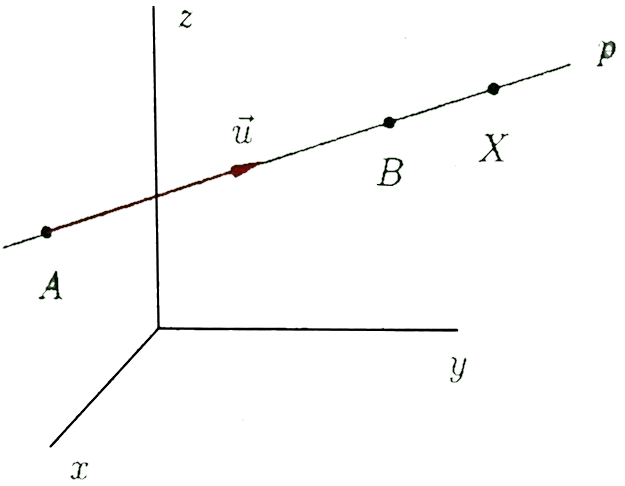
\includegraphics[width=0.4\linewidth]{mai_fig000.png}
    \captionof{figure}{Zadáni přímky. \cite[s.~1]{Musilova2009MA1}
    \label{mai:fig000}}
    \par}
  Veličinou \(t\), takzvaným \emph{parametrem}, který může nabývat všech reálných hodnot, 
  \(t\in\mathbb{R}\), dokážeme popsat všechny vektory \(\overrightarrow{AX}\), jejichž 
  koncový bod \(X\) leží na přímce \(p\). Naopak, žádné jiné body \(X\) než ty, které leží na 
  přímce \(p\), tuto vlastnost nemají. S označením bodů \(A\), \(X\), resp. vektorů 
  \(\vec{u}\), \(\overrightarrow{AX}\) kartézskými souřadnicemi, resp. složkami
  \begin{align*}
                    A &= (x_A,y_A, z_A), \\ 
                    X &=(x,y,z),         \\
              \vec{u} &= (u_1,u_2,u_3),  \\ 
  \overrightarrow{AX} &= (x - x_A, y - y_1A, z-z_A),
  \end{align*}
  dostáváme \textbf{parametrické vyjádřeni přímky} \(p\) ve tvaru
  \begin{equation}\label{MAI:eq_M001}
    p = \left\{(x,y,z)\in\mathbb{R}^3\,|\,
    \begin{matrix}
      x = x_A + tu_1,        \\
      y = y_A + tu_2,        \\
     z = z_A + tu_3,
    \end{matrix}
    \;t\in\mathbb{R}
    \right\}. 
  \end{equation}
  \normalsize
\end{example}
    %---------------------------------------------------------------
    
    Vidíme, že kartézské souřadnice bodu na přímce se vůči souřadnicím bodu \(A\) mění přímo 
    úměrně v závislosti na hodnotě parametru \(t\), tj. závisí na jeho první mocnině. Příslušná 
    závislost se nazývá \textbf{lineární funkcí}.
    
    Obdobně zapíšeme parametrické vyjádření roviny v \(\mathbb{R}^3\):
    
    %--Parametrická vyjádření roviny--------------------------------
    % !TeX spellcheck = cs_CZ
\begin{mathexam}{Parametrická vyjádření roviny}{exam004}
  Rovina v trojrozměrném prostoru \(\mathbb{R}^3\) je zadána třemi body \(A\), \(B\) a \(C\), které
  nesmějí ležet v jedné přímce, popřípadě dvěma body \(A\) a \(B\) a vektorem \(\vec{v}\)
  nerovnoběžným s \(\overrightarrow{AB}\), anebo bodem \(A\) a dvěma nerovnoběžnými směrovými
  vektory \(\vec{u}\) a \(\vec{v}\) (obr. \ref{mai:FIG002}). Všechny tyto typy zadání jsou
  ekvivalentní. Lze volit například \(\vec{u} = \overrightarrow{AB}\), \(\vec{v} =
  \overrightarrow{AC}\). Je-li \(X\) libovolným bodem roviny \(\varrho\), jsou vektory
  \(\overrightarrow{AX}\), \(\vec{u}\) a \(\vec{v}\) \textbf{lineárně závislé}. To znamená, že
  existují taková reálná čísla \(r\) a \(s\), že vektor \(\overrightarrow{AX}\) lze zapsat jako
  lineární kombinaci

  \begin{equation*}
    \overrightarrow{AX} = r\cdot\vec{u} + s\cdot\vec{v}, \qquad r,s \in\mathbb{R}
  \end{equation*}
  Při obdobném zápisu kartézských souřadnic bodů a složek vektorů jako u vyjádření přímky dostaneme
  parametrické vyjádření roviny \(\varrho\)
  \begin{equation*}
    \varrho = \left\{
    \begin{matrix}  
      (x,y,z)\in\mathbb{R}^3  \\
      r, s \in\mathbb{R}
    \end{matrix}
    \,\left\lvert\,
    \begin{matrix}
      x = x_A + ru_1 + sv_1,        \\
      y = y_A + ru_2 + sv_2,        \\
      z = z_A + ru_3 + sv_3,
    \end{matrix}\right.          
    \right\}.
  \end{equation*} 

  { \centering
    \captionsetup{type=figure}
    \luafigure[1]{mai_fig026.pdf}
    \captionof{figure}{Zadání roviny. \cite[s.~3]{Musilova2009MA1}
    \label{mai:FIG002}} \par}

  Toto vyjádření obsahuje opět lineární závislost: Souřadnice \(x\), \(y\) a \(z\) se vůči
  souřadnicím bodu \(A\) mění v závislosti na prvních mocninách parametrů \(r\) a \(s\). Můžeme tak
  hovořit o jakési „vícerozměrné úměře“.
\end{mathexam}
  
    %---------------------------------------------------------------
    
    Všimněme si nyní příkladů linearity z oblasti přírodovědy.
    
    %--Fyzika — Ohmův zákon-----------------------------------------
    % !TeX spellcheck = cs_CZ
% \wikitextrule
\begin{mdframed}[style=mdexam]
  \begin{example}\label{mai:exam035}
    \textbf{Fyzika - Ohmův zákon:}\newline
    Z elektřiny víme, že některé vodiče či elektrické prvky se při průchodu elektrického proudu 
    chovají podle zákona linearity: Proud, který jimi protéká, závisí přímo úměrně na přiloženém 
    napětí (obr. \ref{mai:fig036}). Platí \(I(U) = R^{-1 }U\) s konstantou úměrnosti \(R^{-1}\), kde 
    \(R\) je elektrický odpor vodiče (prvku).

    Pozn. 1: Předpokládáme, že elektrický odpor voltmetru je tak velký, že proud jím procházející je 
    z hlediska přesnosti měření zanedbatelný.
    
    Pozn. 2: Graf závislosti proudu na napětí na obrázku \ref{mai:fig036} může pro vyšší hodnoty 
    napětí vykazovat odchylku od linearity (přímkové závislosti), neboť se prvek při vyšším proudu 
    zahřívá a jeho odpor roste.
    
    {\centering
      \captionsetup{type=figure}
      \luafigure[1]{mai_fig036.png}
      \captionof{figure}{Chování lineárního vodiče (Ohmův zákon). \cite[s.~15]{Musilova2009MA1}
      \label{mai:fig036}}
      \par}  
  \end{example}
\end{mdframed}
    %---------------------------------------------------------------

    %--Fyzika — speciální typy pohybů-------------------------------
    % !TeX spellcheck = cs_CZ
\wikitextrule
\begin{example}\label{mai:exam036}
  \textbf{Fyzika — speciální typy pohybů:}\newline\small
  Při rovnoměrném pohybu tělesa (ať již přímočarém či křivočarém) je dráha, kterou těleso urazí za 
  dobu \(t\), přímo úměrná velikosti jeho rychlosti \(v\), tj. \(s(t) = s_0 + vt\). Při pohybu 
  rovnoměrně zrychleném (zpožděném) je lineární závislost velikosti rychlosti na čase, tj. \(v(t) = 
  v_0 \pm at\) při pohybu přímočarém (\(a\) je velikost zrychlení), nebo \(v(t) = v_0 \pm a_\tau 
  t\) při pohybu křivočarém (\(a_\tau\) je velikost průmětu zrychlení do směru tečny k 
  trajektorii tělesa — tečného zrychlení).
  \normalsize
\end{example}
    %---------------------------------------------------------------
    
  \subsection{Soustavy lineárních rovnic a jejich rychlé řešení}
    Příkladů linearity v přírodě bychom mohli nalézt bezpočet. Vraťme se však k matematice a k 
    problematice uvedené v názvu tohoto odstavce, k soustavám lineárních rovnic. Začněme 
    jednoduchou slovní úlohou ze základní školy:
    
    %--Jeníček a Mařenka kradli ježibabě perník---------------------
    % !TeX spellcheck = cs_CZ
% \wikitextrule
\begin{mdframed}[style=mdexam]
  \begin{example}\label{mai:exam037}
    \textbf{Jeníček a Mařenka kradli ježibabě perník:}\newline
    Dohromady snědli \num{11} perníkových srdíček. Jeníček jich přitom zkonzumoval o \num{3} více
    než Mařenka. Otázka je tradiční - kolik srdíček snědl každý z nich? Označíme-li \(M\) počet
    kousků, které snědla Mařenka a \(J\) počet srdíček, na nichž si pochutnal Jenda, můžeme
    informace zadané v úloze zapsat takto:
    \begin{equation*}
      M + J = 11, \qquad J = M + 3.
    \end{equation*}
    
    Řešení není problémem, snadno vidíme, že \(M = 4\) a \(J = 7\).
  \end{example}
\end{mdframed}
    %---------------------------------------------------------------
    
    O samotné řešení této jednoduché úlohy v tuto chvíli nejde. Pojmenujme si však vztahy, které 
    jsme pro neznámé hodnoty \(M\) a \(J\) ze zadání úlohy dostali. Neznámé vystupují v 
    rovnicích v první mocnině, tedy \emph{lineárně}. Máme \emph{soustavu dvou rovnic} o dvou 
    neznámých \(M\) a \(J\). Úvahu snadno zobecníme: Předpokládejme, že máme neznámé veličiny
    \begin{equation*}
      (x_1, x_2, \ldots, x_n)
    \end{equation*}
    a máme o nich \(m\) informací, které lze zapsat ve tvaru lineárních rovnic (neznámé budou v 
    těchto rovnicích vystupovat v první mocnině),
    \begin{align}
      a_{11}x_1 + a_{12}x_2 + \ldots + a_{1n}x_n &= b_1,     \nonumber           \\
      a_{21}x_1 + a_{22}x_2 + \ldots + a_{2n}x_n &= b_2,     \label{mai:eq002}   \\
      .......................................... &= \ldots   \nonumber           \\
      a_{m1}x_1 + a_{m2}x_2 + \ldots + a_{mn}x_n &= b_m,     \nonumber
    \end{align}
    Soustavu (\ref{mai:eq002}) nazýváme soustavou \(m\) lineárních rovnic o \(n\) neznámých. 
    Označme ji jako \(S\) a pod tímto označením se k ní budeme vracet. Soubory reálných čísel 
    \((a_{ij})\) a \((b_i)\), kde \(1 < i < m\), \(1 \leq j < n\), jsou zadány. Lze je uspořádat 
    do takzvaných \textbf{matic}:
    \begin{equation}\label{mai:eq003}
      \matr{A} =
        \begin{pmatrix}
          a_{11} & a_{12} & \ldots & a_{1n} \\
          a_{21} & a_{22} & \ldots & a_{2n} \\
          \ldots & \ldots & \ldots & \ldots \\
          a_{m1} & a_{m2} & \ldots & a_{mn}          
        \end{pmatrix},
        \overline{\matr{B}} =
        \begin{pmatrix}
          b_1     \\
          b_2     \\
          \ldots  \\
          b_m 
        \end{pmatrix}
    \end{equation}
    
    Matice \(\matr{A}\) je typu \(m/n\), má \(m\) řádků a \(n\) sloupců, \(i\) je řádkový index a 
    \(j\) je sloupcový index. Matice \(\overline{\matr{B}}\) je typu \(m/1\) (\(m\) řádků a jeden 
    sloupec), hovoříme také o sloupcové matici. Soustavu \(S\) můžeme zapsat zkráceně pomocí 
    maticového násobení (podrobněji viz později odstavec \ref{mai:IchapIIsecIII}):
    \begin{equation*}
      \matr{A} \cdot \matr{X} = \matr{B}, \qquad \text{nebo}
    \end{equation*}  
    \begin{equation}\label{mai:eq004}
        \begin{pmatrix}
          a_{11} & a_{12} & \ldots & a_{1n} \\
          a_{21} & a_{22} & \ldots & a_{2n} \\
          \ldots & \ldots & \ldots & \ldots \\
          a_{m1} & a_{m2} & \ldots & a_{mn}
        \end{pmatrix}
        \cdot
        \begin{pmatrix}
          x_1     \\
          x_2     \\
          \ldots  \\
          x_m 
       \end{pmatrix}
        =
       \begin{pmatrix}
            b_1     \\
            b_2     \\
            \ldots  \\
            b_m 
          \end{pmatrix}
    \end{equation}
    V tuto chvíli vysvětlíme podstatu maticového násobení jen technicky: Násobit mezi sebou  můžeme matici 
    \(\matr{A} = (a_{ij})\) typu \(m/n\) (levý činitel) a matici \(\matr{A} = (c_{jk})\) typu 
    \(n/p\) (pravý činitel, činitele nelze zaměňovat). Výsledkem je matice \(\matr{A} = (d_{ik})\) 
    typu \(m/p\), jejíž prvky se počítají podle předpisu
    \begin{equation}\label{mai:eq005}
      d_{ik} = \sum_{j=1}^{n} a_{ij}\cdot c_{jk}.
    \end{equation}
    
    Z tohoto obecného předpisu vidíme, že levé strany soustavy \(S\) lze interpretovat ve tvaru 
    součinu matice \(A\) typu \(m/n\) s maticí neznámých typu \((n/1)\), výsledkem je matice 
    pravých stran \(\overline{\matr{B}}\), která je typu \(m/1\). Matice \(\matr{A}\) se nazývá 
    \textbf{maticí soustavy}. Matice, která vznikne jejím \emph{rozšířením} o sloupec pravých 
    stran, tj.
    \begin{equation}\label{mai:eq006}
      \matr{B} = (\matr{A}|\overline{\matr{B}}) =
      \left(
        \begin{array}{cccc|c}
          a_{11} & a_{12} & \ldots & a_{1n} & b_1    \\
          a_{21} & a_{22} & \ldots & a_{2n} & b_2    \\
          \ldots & \ldots & \ldots & \ldots & \ldots \\
          a_{m1} & a_{m2} & \ldots & a_{mn} & b_m
        \end{array}
      \right)
    \end{equation}
    je pak \textbf{rozšířenou maticí soustavy}. Je-li sloupec pravých stran soustavy tvořen 
    samými nulami, nazývá se soustava \textbf{homogenní}, v opačném případě \textbf{nehomogenní}. 
    Řešením soustavy \(S\) nazýváme každou \(n\)-tici \((x_i, x_2,\ldots, x_n)\), která soustavu 
    \(S\) splňuje. Cílem je najít všechna řešení soustavy \(S\). Abychom řešení nalezli, musíme 
    soustavu upravovat, zjednodušovat. Prováděné úpravy mají vést k jednodušší, avšak 
    ekvivalentní soustavě rovnic, tj. takové, která má naprosto stejný soubor všech řešení jako 
    soustava původní. Takové úpravy nazýváme \textbf{ekvivalentními}. Dvě základní, pomocí nichž 
    lze uskutečnit všechny ostatní, jsou
    \begin{itemize}\addtolength{\itemsep}{-0.5\baselineskip}
      \item vynásobení libovolné, například \(i\)-té, rovnice libovolným \emph{nenulovým} číslem,
      \item přičtení \(i\)-té rovnice vynásobené libovolným číslem k \(l\)-té rovnici.
    \end{itemize} 
    V soustavě lze samozřejmě také měnit pořadí rovnic. Tato úprava je rovněž ekvivalentní. 
    Nevypisujeme ji však zvlášť proto, že ji lze realizovat pomocí vhodně zvolené posloupnosti 
    základních dvou úprav.
    
    Abychom nemuseli soustavu stále opisovat i s neznámými, provádíme obvykle ekvivalentní 
    úpravy jen s maticí \(\matr{B} = (\matr{A}|\overline{\matr{B}})\) (každý řádek této matice 
    představuje jednu rovnici soustavy \(S\)). Může se stát, že soustava má právě \emph{jedno 
    řešení}, jako tomu bylo v  úloze o Mařence a Jeníčkovi. Také nemusí mít \emph{řešení žádné}, 
    jako například soustava \(x + y = 0\), \(x + y = 1\) (součet dvou čísel nemůže nabývat současně 
    dvou různých hodnot). A třeba má také řešení \emph{nekonečně mnoho} (řešením soustavy jedné 
    rovnice o dvou neznámých \(x + y = 1\) jsou všechny dvojice tvaru \((x, 1 - x)\), kde \(x\) je 
    libovolné). A může mít soustava \(S\) třeba právě dvě řešení? Prostřednictvím následujícího 
    příkladu ukážeme metodu, která vede velmi rychle k nalezení všech řešení a umožňuje také 
    vyslovit obecné závěry o jejich vlastnostech a počtu. Jedná se o \textbf{Gaussovu eliminační 
    metodu}.

    %Gaussova eliminační metoda-------------------------------------
    \begin{mathexam}{Gaussova eliminační metoda}{exam038}
  Je zadána soustava tří (\(m = 3\)) rovnic o pěti (\(n = 5\)) neznámých:
  \begin{alignat*}{7}
       x_1 &+ 2x_2 &-  x_3 &+  x_4 &- 5x_5 &=  &&0, \\
     -2x_1 &- 4x_2 &+ 2x_3 &+ 4x_4 &+ 4x_5 &= -&&6, \\
      -x_1 &- 2x_2 &+  x_3 &+ 5x_4 &-  x_5 &=  &&6.
  \end{alignat*}
  Budeme provádět ekvivalentní úpravy matice \(\matr{B}\) tak, abychom ji zjednodušovali.
  Ekvivalenci matic budeme označovat znakem \(\sim\). 
  \begingroup
    \renewcommand\arraystretch{1.0}
    \renewcommand\arraycolsep{3pt}
    \begin{equation*}
      \matr{B} = (\matr{A}\lvert\overline{\matr{B}}) =
      \left(
        \begin{array}{rrrrr|r}
           1 &  2 & -1 & 1 & -5 &  0    \\
          -2 & -4 &  2 & 4 &  4 & -6    \\
          -1 & -2 &  1 & 5 & -1 &  6
        \end{array}
      \right).
    \end{equation*}
  \endgroup
  V prvním řádku je na první pozici jednička. Toho využijeme k snadné „likvidaci“, tedy eliminaci,
  prvních prvků v druhém a třetím řádku pomocí elementárních úprav. Provedeme tyto dvě úpravy:
  první řádek vynásobený číslem \num{2} přičteme k druhému řádku, první řádek přičteme ke třetímu
  řádku. Dostaneme
  \begingroup
    \renewcommand\arraystretch{1.0}
    \renewcommand\arraycolsep{3pt}
    \begin{equation*}
      \matr{B} \sim
      \left(
        \begin{array}{rrrrr|r}
          1 &  2 & -1 & 1 & -5 &  0         \\
          \bm{0} &  0 &  0 & 6 & -6 & -6    \\
          \bm{0} &  0 &  0 & 6 & -6 &  6
        \end{array}
      \right).
    \end{equation*}
  \endgroup  
  Vidíme, že jsme v druhém i třetím řádku dostali na první sloupcové pozici nulu (tučná). (Nuly na
  dalších  pozicích vznikly náhodou, vlivem jednoduchosti zadání.) Nyní vynásobíme druhý i třetí
  řádek číslem (\num{1/6}):
  \begingroup
    \renewcommand\arraystretch{1.0}
    \renewcommand\arraycolsep{3pt}    
    \begin{equation*}
      \matr{B} \sim
      \left(
        \begin{array}{rrrrr|r}
                1 &  2 & -1 & 1 & -5 &  0    \\
                0 &  0 &  0 & 1 & -1 & -1    \\
                0 &  0 &  0 & 1 & -1 &  1
        \end{array}
      \right).
    \end{equation*}
  \endgroup  
  Přestože již nyní vidíme, že soustava nemá řešení (rovnice druhého a třetího řádku znějí \(x_4 -
  x_5 = - 1\) a \(x_4 -x_5 = 1\), takže jim nevyhovuje žádná dvojice čísel \((x_4, x_5)\)), budeme
  v eliminaci pokračovat. Další úpravy se již týkají pouze druhého a třetího řádku. Druhý řádek
  vynásobený (\num{-1}) přičteme ke třetímu. Pak

  \begingroup
  \renewcommand\arraystretch{1.0}
  \renewcommand\arraycolsep{3pt}
    \begin{equation*}
      \matr{B} \sim
      \left(
        \begin{array}{rrrrr|r}
                1 &  2 & -1 & 1      & -5 &  0    \\
                0 &  0 &  0 & 1      & -1 & -1    \\
                0 &  0 &  0 & \bm{0} &  0 &  2
        \end{array}
      \right).
    \end{equation*}
  \endgroup  
  Získáváme tak ekvivalentní soustavu rovnic
  \begin{alignat*}{5}
        x_1 + 2x_2 - x_3 &+  x_4 &- 5x_5 &=  &&0, \\
                         &+  x_4 &-  x_5 &= -&&1, \\
                         &       &     0 &=  &&2.
  \end{alignat*}
  V poslední rovnici je ihned vidět rozpor - soustava nemá řešení
\end{mathexam}
    %---------------------------------------------------------------

    Na základě výsledného tvaru matice soustavy a rozšířené matice soustavy získané ekvivalentními 
    úpravami soustavy \(S\) nyní formulujeme obecné kritérium pro to, aby soustava S měla
    vůbec nějaké řešení. Matice \(\matr{A}\) i \(\matr{B}\) se po provedení ekvivalentních úprav 
    dostaly do velmi jednoduchého tvaru, který připomíná schodiště obrácené „vzhůru nohama“, 
    odmyslíme-li si nuly v levé části jednotlivých řádků (následující zápis pouze usnadňuje 
    názornou představu, znak ekvivalence již psát nemůžeme):
    \begin{equation*}
      \matr{A} \ldots
      \left(
        \begin{array}{rrrrr}
                1 &  2 & -1 & 1      & -5     \\
                  &    &    & 1      & -1     \\
 
        \end{array}
      \right),
      \qquad
      \matr{B} \ldots
      \left(
        \begin{array}{rrrrr|r}
                1 &  2 & -1 & 1      & -5 &  0    \\
                  &    &    & 1      & -1 & -1    \\
        \end{array}
      \right).
    \end{equation*}
    
    Všimněme si, že „schodiště“ jsou nepravidelná, pokud jde o šířku schodů, výška všech schodů
    je však stejná - jeden řádek. Tímto způsobem je dán \emph{schodovitý tvar} matice \(\matr{A}\), 
    resp. \(\matr{B}\). Úzce s ním souvisí důležitá charakteristika matice, která je nezávislá jak 
    na provedených úpravách tak na výsledném schodovitém tvaru. Je to hodnost matice, definovaná 
    takto:
    
    \textbf{Hodnost} matice je počet nenulových řádků jejího schodovitého tvaru.
    
    V našem příkladu je hodnost matice \(A\) soustavy \(S\) rovna dvěma, hodnost matice rozšířené 
    \(\matr{B}\) je rovna třem. Píšeme
    \begin{equation*}
      h(\matr{A}) = 2,\qquad h(\matr{B}) = 3.
    \end{equation*}
    
    \begin{note}
      Lze získat schodovitý tvar různými posloupnostmi ekvivalentních úprav je zřejmé. Uvědomme si 
      však, že ani výsledný schodovitý tvar není určen jednoznačně - stačí třeba vynásobit některý 
      řádek dvěma a výsledná matice ekvivalentní s původní je rovněž schodovitá. Poněvadž má matice 
      \(\matr{B}\) o jeden sloupec více než matice \(\matr{A}\), platí vždy \(h(\matr{A}) < 
      h(\matr{B})\). V případě \(h(\matr{A}) < h(\matr{B})\) pak \(h(\matr{A}) = h(\matr{B}) - 1\). 
      Jak názorně ukazuje náš příklad, má pro \(h(\matr{A}) < h(\matr{B})\) některá z rovnic 
      ekvivalentní soustavy tvar \(0 = 1\), soustava tedy nemá řešení. Můžeme tak formulovat 
      kritérium (podmínku nutnou a postačující) řešitelnosti soustavy lineárních rovnic.
    \end{note}
    
    \begin{lemma}\label{mai:lemma001}
      (\textbf{Frobeniova}): Soustava lineárních rovnic má řešení právě tehdy, je-li hodnost její 
      matice rovna hodnosti matice rozšířené.
    \end{lemma}
    
    Ihned vidíme, že homogenní soustava má podle této věty řešení vždy, neboť poslední sloupec její 
    rozšířené matice je složen ze samých nul. Skutečně, jedním ze souboru řešení každé
    homogenní soustavy je \(n\)-tice
    \begin{equation*}
      (x_1, x_2, \ldots, x_n) = (0, 0, \ldots, 0),
    \end{equation*}
    zvaná \textbf{triviální řešení}.
    
    Nyní se vraťme k otázce, jak zjistit, kolik řešení má daná soustava, a jak je všechna popsat.
    Poslouží nám příklad \ref{mai:exam038} v mírné obměně spočívající v záměně koeficientu \(b_3\) 
    z hodnoty \num{6} na \num{-6}.
    
    %Ještě jednou Gaussova eliminační metoda------------------------
    % !TeX spellcheck = cs_CZ
\wikitextrule
\begin{example}\label{mai:exam039}
  \textbf{Ještě jednou Gaussova eliminační metoda}\newline\small
  Je zadána soustava rovnic:
  \begin{alignat*}{7}
      x_1 &+ 2x_2 &-  x_3 &+  x_4 &- 5x_5 &=  &&0, \\
    -2x_1 &- 4x_2 &+ 2x_3 &+ 4x_4 &+ 4x_5 &= -&&6, \\
     -x_1 &- 2x_2 &+  x_3 &+ 5x_4 &-  x_5 &= -&&6.
  \end{alignat*}
  Rozšířená matice soustavy má nyní tvar 
  \begin{equation*}
    \matr{B} = (\matr{A}|\overline{\matr{B}}) =
    \left(
      \begin{array}{rrrrr|r}
         1 &  2 & -1 & 1 & -5 &  0    \\
        -2 & -4 &  2 & 4 &  4 & -6    \\
        -1 & -2 &  1 & 5 & -1 & -6
      \end{array}
    \right).
  \end{equation*}
  Stejné ekvivalentní úpravy jako v příkladu \ref{mai:exam038} vedou nyní k výsledku
  \footnotesize %\small \scriptsize \tiny
  \begin{equation*}
    \matr{B} \sim
    \left(
      \begin{array}{rrrrr|r}
         1 &  2 & -1 & 1 & -5 &  0         \\
         \bm{0} &  0 &  0 & 6 & -6 & -6    \\
         \bm{0} &  0 &  0 & 6 & -6 & -6
      \end{array}
    \right) \sim
    \left(
      \begin{array}{rrrrr|r}
              1 &  2 & -1 & 1 & -5 &  0    \\
              0 &  0 &  0 & 1 & -1 & -1    \\
              0 &  0 &  0 & 1 & -1 & -1
      \end{array}
    \right) \sim
    \left(
      \begin{array}{rrrrr|r}
              1 &  2 & -1 & 1      & -5 &  0    \\
              0 &  0 &  0 & 1      & -1 & -1    \\
              0 &  0 &  0 & \bm{0} &  0 &  0
      \end{array}
    \right).
  \end{equation*}\normalsize
  Nyní platí \(h(\matr{A}) = h(\matr{B}) = 2\). Podle Frobeniovy věty \ref{mai:lemma001} tedy 
  soustava určitě má řešení. Ekvivalentní soustava má tvar
  \begin{alignat*}{5}
         x_1 + 2x_2 - x_3 &+  x_4 &- 5x_5 &=  &&0, \\
                          &+  x_4 &-  x_5 &= -&&1, \\
                          &       &     0 &=  &&0.
  \end{alignat*}
  Poslední rovnice je identitou a můžeme ji vypustit. Máme pět neznámých a jen dvě nezávislé 
  rovnice. Dvě z neznámých tedy můžeme vyjádřit pomocí zbývajících. Postupujeme „odzadu“ , začínáme 
  druhou, jednodušší, rovnicí:
  \begin{align*}
                                                x_4 &= -1 + x_5,                \\
    x_1 = - 2x_2 + x_3 - x_4 + 5x_5 \Rightarrow x_1 &= -2x_2 + x_3 + 4x_5 + 1.
  \end{align*}
  Za neznámé vystupující na pravé straně, tj. \(x_2\), \(x_3\) a \(x_5\), můžeme dosazovat cokoli a 
  vždycky se k nějakým hodnotám \(x_1\) a \(x_4\) dopočítáme. Všechna řešení soustavy \(S\) proto 
  můžeme zapsat v obecném tvaru
  \begin{equation}\label{mai:eq040}
    (-2x_2 + x_3 + 4x_5 + 1, x_2, x_3, x_5 - 1, x_5).
  \end{equation}
  \normalsize
\end{example}
    %---------------------------------------------------------------
    
    Soubor řešení ve tvaru (\ref{mai:eq040}) se nazývá obecným řešením soustavy. Jeho jednotlivé 
    prvky, jednotlivá konkrétní řešení soustavy, jsou dány volbou volných neznámých \(x_2\), 
    \(x_3\) a \(x_5\). Také z příkladu \ref{mai:exam039} lze učinit obecný závěr:
    
    \begin{lemma}\label{mai:lemma002}
      Nechť pro soustavu \(m\) lineárních rovnic o \(n\) neznámých platí \(h(\matr{A}) = 
      h(\matr{B}) = h\). Pak její obecné řešení závisí (lineárně) na \(d = n - h\) volných 
      neznámých.
    \end{lemma}
    
    Číslo \(d\) se nazývá \textbf{dimenze prostoru řešení soustavy}. Tento pojem ještě podrobněji 
    vysvětlíme později.
    
    Nyní již snadno zodpovíme otázku, čím je dána mohutnost souboru řešení soustavy lineárních 
    rovnic, tj. kolik má taková soustava řešení. Možnosti jsou pouze:
    \begin{itemize}
      \item žádné řešení - pro \(h(\matr{A}) \neq h(\matr{B})\),
      \item právě jedno řešení - pro \(h = h(\matr{A}) = h(\matr{B})\) a současně \(h = n\), takže 
            nezbývá žádná volná neznámá,
      \item nekonečně mnoho řešení - pro \(h = h(\matr{A}) = h(\matr{B})\) a současně \(h < n\),  
            kdy máme k dispozici \(d = n - h\) volných neznámých.
    \end{itemize}    
    Že by tedy třeba měla soustava právě dvě, tři či osmnáct řešení není možné.
    
    Jakési zvláštní postavení můžeme přisoudit homogenním soustavám. Ty mají, jak jsme se
    již přesvědčili, řešení vždy, alespoň to triviální, složené ze samých nul. Zajímejme se o 
    situaci, kdy má homogenní soustava i jiná, netriviální, řešení. U homogenní soustavy je 
    hodnost její matice vždy shodná s hodností matice rozšířené, \(h = h(\matr{A}) = h(\matr{B})\). 
    Je-li navíc \(h = n\), má podle obecného tvrzení \ref{mai:lemma002} soustava právě jedno 
    řešení, jímž nutně je řešení triviální. V opačném případě, tj. pro \(h < n\), máme opět k 
    dispozici \(d = n - h\) volných neznámých, a tedy nekonečně mnoho netriviálních řešení. 
    Všimněme si ještě jedné zajímavosti u homogenní soustavy. Jsou-li dvě \(n\)-tice čísel \(X = 
    (x_1, x_2, \ldots, x_n)\) a \(\overline{X} = (\overline{x}_1, \overline{x}_2, \ldots, 
    \overline{x}_n)\) jejím řešením, pak také \(n\)-tice vytvořená jako jejich lineární kombinace
    \begin{equation*}
      \alpha\cdot X + \overline{\alpha}\cdot\overline{X} = 
        (\alpha x_1, \alpha x_2, \ldots, \alpha x_n) + 
        (\overline{\alpha}\,\overline{x}_1, 
        \overline{\alpha}\,\overline{x}_2, \ldots, 
        \overline{\alpha}\,\overline{x}_n)
    \end{equation*}
    kde \(\alpha\) a \(\overline{\alpha}\) jsou libovolná čísla, je \emph{řešením soustavy}. 
    Možnost tohoto „lineárního kombinování“ připadá samozřejmě v úvahu pro libovolný počet 
    libovolných řešení soustavy. Fyzik by řekl, že soustava vyhovuje principu superpozice. 
    Soustava nehomogenní tu to vlastnost nemá „vinou“ nenulového sloupce 
    pravých stran.
    
    \subsection{Přímky a roviny - lineární geometrické útvary}
      Vraťme se ještě na chvíli k linearitě v geometrii a všimněme si problematiky vzájemné polohy
      přímek a rovin. Procvičíme si na ní mimo jiné i řešení soustav lineárních rovnic. V odstavci 
      \ref{mai:IchapIIsecI} jsme odvodili parametrické vyjádření přímky a roviny v trojrozměrném 
      prostoru. Nyní se pokusíme z těchto vyjádření vyloučit parametry a získat obecné rovnice 
      přímky a roviny, které již budou obsahovat pouze kartézské souřadnice bodů ležících v 
      příslušné přímce či rovině. Začněme případem roviny.

      %--Obecná rovnice roviny----------------------------------------
      % !TeX spellcheck = cs_CZ
\wikitextrule
\begin{example}\label{mai:exam040}
  \textbf{Obecná rovnice roviny}\newline\small
  Parametrické rovnice roviny z příkladu \ref{mai:exam004} můžeme chápat jako soustavu tří rovnic o 
  dvou neznámých:
  \begin{align*}
      ru_1 + sv_1 &= x - x_A, \\
      ru_2 + sv_2 &= y - y_A, \\
      ru_3 + sv_3 &= z - z_A, 
  \end{align*}
  kde neznámými jsou parametry \(r\) a \(s\). Z geometrického významu této soustavy je zřejmé, že 
  pro každý bod \(X = (x, y, z)\), který leží v rovině \(\varrho\), bude soustava mít jako řešení 
  právě jednu dvojici parametrů \((r, s)\) (pro body, které v rovině neleží, soustava řešení nemá). 
  Vypočteme parametry \(r\) a \(s\) například z prvních dvou rovnic. Předpokládejme, že \(u_1 \neq 
  0\), a upravujme matici soustavy:
  
  \begin{equation*}
    \left(
      \begin{array}{rr|r}
         u_1 &  v_1  &  x-x_A         \\
         u_2 &  v_2  &  y-y_A
      \end{array}
    \right) \sim
    \left(
      \begin{array}{cc|c}
              u_1 &  v_1               & x - x_A     \\
              0   &  u_1v_2 - u_2v_1   & (y-y_A)u_1 - (x-x_A)u_2
      \end{array}
    \right).
  \end{equation*}
  odkud pro \((u_1v_2 — u_2v_1) \neq 0\) dostaneme
  \begin{equation*}
    r = - \dfrac{(y-y_A)v_1 - (x-x_A)v_2}{u_1v_2 - u_2v_1}, \qquad 
    s =   \dfrac{(y-y_A)u_1 - (x-x_A)u_2}{u_1v_2 - u_2v_1}
  \end{equation*}
  Dosadíme-li získané hodnoty do třetí rovnice (dá to trochu práce), dostáváme obecnou  rovnici roviny 
  \(\varrho\)
  \begin{subequations} % \label{mai:eq041}
    \begin{equation}\label{mai:eq041a}
      ax + by + cz + d= 0,
    \end{equation}
    \begin{equation}\label{mai:eq04b}
      a = u_2v_3 - u_3v_2, \qquad b = u_3v_1 - u_1v_3, \qquad c = u_1v_2 - u_2v_1,
    \end{equation}
    \begin{equation}\label{mai:eq041c}
      d = (u_2v_3 - u_3v_2)x_A - (u_3v_1 - u_1v_3)y_A - (u_1v_2 - u_2v_1)z_A.
    \end{equation}
  \end{subequations}
  Při tomto výpočtu vyvstaly některé problémy. Pokusme se je vyřešit:
  \begin{itemize}
    \item Aby získaná rovnice opravdu představovala nějakou rovinu, musí v ní zůstat alespoň jedna 
          ze souřadnic \(x, y, z\). Alespoň jedno z čísel \(a, b, c\) by tedy mělo být nenulové. 
          Dokažte, že tomu tak opravdu je, a využijte při tom skutečnosti, že vektory \(\vec{u}\) a 
          \(\vec{v}\) nesmí být rovnoběžné. Co znamená předpoklad \((u_1v_2 - u_2v_1) \neq 0\)?
    \item Předpokládali jsme, že \(u_1 \neq 0\). Jak budeme postupovat, nebude-li tento předpoklad  
          splněn? Lze v tomto případě použít obecné výrazy získané pro \(r\) a \(s\)?
  \end{itemize}
  \normalsize
\end{example}
      %---------------------------------------------------------------

      %--Obecná rovnice přímky----------------------------------------
      % !TeX spellcheck = cs_CZ
% \wikitextrule
\begin{mdframed}[style=mdexam]
  \begin{example}\label{mai:exam041}
    \textbf{Obecná rovnice přímky}\newline
    Přímku \(p\) si snadno představíme jako průsečnici dvou nerovnoběžných rovin \(\varrho\) a 
    \(\sigma\). Jejich rovnice tvoří soustavu, která představuje obecné rovnice přímky
      \begin{align*}
        \varrho &= \{(x, y, z)\in\mathbb{R}^3\mid a_1x+ b_1y+ c_1z+ d_1 = 0 \}  \\ 
        \sigma  &= \{(x, y, z)\in\mathbb{R}^3\mid a_2x+ b_2y+ c_2z+ d_2 = 0 \}, 
      \end{align*}
    Zkusme přijít na to, co musí platit pro koeficienty v rovnicích rovin, aby byly nerovnoběžné. 
    Jedna a táž přímka může být zadána různými dvojicemi nerovnoběžných rovin. Všechny roviny, které 
    přímkou \(p\) procházejí, tvoří geometrický útvar zvaný \textbf{svazek rovin prvního druhu}, 
    přímka sama je \textbf{osou} svazku. 
  \end{example}
\end{mdframed}
      %---------------------------------------------------------------
      
      %--Vektor rovnoběžný s rovinou----------------------------------
      % !TeX spellcheck = cs_CZ
\wikitextrule
\begin{example}\label{mai:exam042}
  \textbf{Vektor rovnoběžný s rovinou}\newline\small
   Ja k poznáme, zda je vektor \(\vec{u} = (u_1, u_2, u_3)\) rovnoběžný s rovinou \(ax + by + cz + 
   d = 0\)? Pokud vektor \(\vec{u}\) s rovinou rovnoběžný je, pak zcela jistě existují v této 
   rovině dva body \(A = (x_A, y_A, z_A)\) a \(B = (x_B, y_B, z_B)\) tak, že \(\overrightarrow{AB} 
   = \vec{u} = (x_B - x_A, y_B - y_A, z_B - z_A)\). Tyto body splňují rovnici roviny, tj.
   \begin{equation*}
     ax_A + by_A + cz_A + d = 0,\qquad ax_B + by_B + cz_B + d = 0.
   \end{equation*}
   Odečtením rovnic dostaneme kritérium rovnoběžnosti vektoru s rovinou \(au_1 + bu_2+ cu_3 = 0\).
   \normalsize
\end{example}
      %---------------------------------------------------------------
  
      Máme připraveno vše pro řešení otázky vzájemné polohy přímek a rovin.

      %--Vzájemná poloha tří rovin------------------------------------
      % !TeX spellcheck = cs_CZ
\wikitextrule
\begin{example}\label{mai:exam043}
  \textbf{Vzájemná poloha tří rovin}\newline\small
  Zapojme geometrickou představivost a uvažujme, jakou vzájemnou polohu mohou mít tři roviny
  \begin{align*}
    \varrho: a_1x + b_1y + c_1z + d_1 &= 0, \\
    \sigma : a_2x + b_2y + c_2z + d_2 &= 0, \\
    \tau   : a_3x + b_3y + c_3z + d_3 &= 0,
  \end{align*}
  Současně si uvědomme, že předchozí soustava je soustavou lineárních rovnic o neznámých \(x\), 
  \(y\) a \(z\), představujících souřadnice společných bodů rovin \(\varrho\), \(\sigma\) a 
  \(\tau\). Soustava je charakterizována maticí
  \begin{equation}\label{mai:eq043}
    \matr{B} = (\matr{A}|\overline{\matr{B}}) =
    \left(
      \begin{array}{rrr|r}
         a_1 & b_1 & c_1 & -d_1    \\
         a_2 & b_2 & c_2 & -d_2    \\
         a_3 & b_3 & c_3 & -d_3
      \end{array}
    \right).
  \end{equation}
  Jsou tyto možnosti:
  \begin{itemize}
    \item Roviny mají společný právě jeden bod. V tomto případě musí mít soustava (\ref{mai:eq043}) 
          právě jedno řešení, a tedy \(h(\matr{A}) = h(\matr{B}) = 3\). (Útvar, který by vytvořily 
          všechny roviny procházející tímto bodem, se nazývá \textbf{trs rovin prvního druhu}, 
          společný bod je vrchol trsu.)
    \item Roviny mají společnou přímku. Řešení soustavy (\ref{mai:eq043}) bude v takovém případě 
          závislé na jedné volné neznámé (parametr bodů na společné přímce), takže \(h(\matr{A}) = 
          h(\matr{B}) = 2\). (Útvar, který by vytvořily všechny roviny procházející touto přímkou, 
          jsme před chvílí nazvali \textbf{svazkem rovin prvního druhu}, společná přímka je 
          \textbf{osou} svazku.)
    \item Roviny jsou totožné. Řešení soustavy (\ref{mai:eq043}) je popsáno dvěma volnými neznámými 
          (parametry bodů ve společné rovině), je tedy \(h(\matr{A}) = h(\matr{B}) = 1\).
    \item Roviny nemají společný žádný bod, mají však společný právě jeden směr (představme si 
          například nekonečně dlouhý stan „áčko“, v němž jedna z rovin tvoří podlážku a zbylé dvě 
          jsou stěnami). Společný směr \(\vec{u}\) je řešením homogenní soustavy rovnic (příklad 
          \ref{mai:exam043})
          \begin{align}\label{mai:eq044}
            a_1u_1 + b_1u_2+ c_1u_3 &= 0, \\
            a_2u_1 + b_2u_2+ c_2u_3 &= 0, \\
            a_3u_1 + b_3u_2+ c_3u_3 &= 0.
          \end{align}
           jejíž řešení musí být popsáno jednou volnou neznámou, tj. \(h(\matr{A}) = 2\). Původní 
           nehomogenní soustava (\ref{mai:eq043}) pro společné body rovin však řešení nemá, je tedy 
           \(h(\matr{B}) = 3\). (Útvar, který by vytvořily všechny roviny obsahující společný směr, 
           se nazývá \textbf{trs rovin druhého druhu}.)
    \item Roviny jsou rovnoběžné, nemají však žádný společný bod. Znamená to, že mají společné 
          dva nezávislé směry, řešení homogenní soustavy (\ref{mai:eq044}) obsahuje dvě volné 
          neznámé a platí \(h(\matr{A}) = 1\), \(h(\matr{B}) = 2\).
  \end{itemize}
  \normalsize
\end{example}
      %---------------------------------------------------------------

      %--Vzájemná poloha dvou přímek----------------------------------
      % !TeX spellcheck = cs_CZ
\wikitextrule
\begin{example}\label{mai:exam044}
  \textbf{Vzájemná poloha dvou přímek}\newline\small
  Dvě přímky \(p\) a \(q\) jsou určeny dvěma dvojicemi rovin. Jejich společné body jsou tedy 
  řešením soustavy čtyř lineárních rovnic o třech neznámých (pišme rovnou rozšířenou matici 
  soustavy):
  \begin{equation}\label{mai:eq045}
    \matr{B} = (\matr{A}|\overline{\matr{B}}) =
    \left(
      \begin{array}{rrr|r}
         a_1 & b_1 & c_1 & -d_1    \\
         a_2 & b_2 & c_2 & -d_2    \\
         a_3 & b_3 & c_3 & -d_3    \\
         a_4 & b_4 & c_4 & -d_4
      \end{array}
    \right).
  \end{equation}
  Protože soustava obsahuje rovnice dvojic nerovnoběžných rovin, je \(h(\matr{A}) \geq 2\) 
  (zdůvodněte podrobněji). Možnosti vzájemné polohy přímek \(p\) (první dvě rovnice) a \(q\) (druhé 
  dvě rovnice) jsou tyto:
  \begin{itemize}
    \item Přímky jsou mimoběžné, nemají tedy žádný společný bod a roviny, které je určují, nemají 
          žádný společný směr. Soustava (\ref{mai:eq045}) nemá řešení, odpovídající homogenní 
          soustava pak rovněž ne, kromě řešení triviálního. Je tedy \(h(\matr{A}) = 3\), 
          \(h(\matr{B}) = 4\).
    \item Přímky jsou různoběžné, mají tedy společný právě jeden bod. Soustava (\ref{mai:eq045}) má 
          právě jedno řešení, a proto \(h(\matr{A}) = h(\matr{B}) = 3\).
    \item Přímky jsou rovnoběžné. Nemají tedy žádný společný bod, soustava nemá řešení, ale roviny, 
          které je určují, mají společný směr. To odpovídá situaci \(h(\matr{A}) = 23\), 
          \(h(\matr{B}) = 3\).
    \item Přímky jsou totožné. Řešení soustavy je popsáno jednou volnou neznámou, tj. \(h(\matr{A}) 
          = h(\matr{B}) = 2\)
  \end{itemize}
  \normalsize
\end{example}
      %---------------------------------------------------------------
      
      %--Vzájemná poloha přímky a roviny------------------------------
      % !TeX spellcheck = cs_CZ
\wikitextrule
\begin{example}\label{mai:exam045}
  \textbf{Vzájemná poloha přímky a roviny}\newline\small
  Tuto úlohu převeďme na problém vzájemné polohy tří rovin a odpovězme si sami. Společně vyřešíme 
  konkrétní případ. Rozhodněme o vzájemné poloze přímky a roviny, najděme jejich společné body a 
  směry:
  \begin{align*}
    p       &: x + y + z + 5 = 0, \qquad 2x + 3y + 6z - 10 = 0 \\
    \varrho &: y + 4z + 17   = 0.
  \end{align*}
  \begin{equation*}
    \matr{B} = (\matr{A}|\overline{\matr{B}}) =
    \left(
      \begin{array}{rrr|r}
         1 & 1 & 1 & -5    \\
         2 & 3 & 6 &  10   \\
         0 & 1 & 4 & -17
      \end{array}
    \right)\sim
    \left(
      \begin{array}{rrr|r}
         1 & 1 & 1 & -5    \\
         0 & 1 & 4 &  20   \\
         0 & 1 & 4 & -17
      \end{array}
    \right)\sim
    \left(
      \begin{array}{rrr|r}
         1 & 1 & 1 & -5    \\
         0 & 1 & 4 &  20   \\
         0 & 0 & 0 & -37
      \end{array}
    \right).
  \end{equation*}
  Matice \(\matr{A}\) i \(\matr{B}\) jsme upravili do schodovitého tvaru. Vidíme, že \(h(\matr{A}) 
  = 2\), \(h(\matr{B}) = 3\). Soustava nemá řešení přímka \(p\) a rovina \(\varrho\) nemají žádný 
  společný bod. Jediná možnost, jak to zařídit, je, že přímka \(p\) je s rovinou \(\varrho\) 
  rovnoběžná. Mají společný směr, který je řešením homogenní soustavy o matici
  \begin{equation*}
    \matr{A} =
    \left(
      \begin{array}{ccc}
         1 & 1 & 1   \\
         2 & 3 & 6   \\
         0 & 1 & 4 
      \end{array}
    \right)\sim
    \left(
      \begin{array}{ccc}
         1 & 1 & 1   \\
         0 & 1 & 4   \\
         0 & 0 & 0 
      \end{array}
    \right).
  \end{equation*}
  Schodovitý tvar matice odpovídá ekvivalentní soustavě rovnic
  \begin{equation*}
    u_1 + u_2 + u_3 = 0,\qquad u_2 + 4u_3 = 0,
  \end{equation*}
  jejíž řešení je tvaru \((u_1, u_2, u_3) = (3u_3, -4u_3, u_3)\). Společný směr přímky \(p\) a 
  roviny \(\varrho\) je tedy určen například směrovým vektorem \((3, -4, 1)\) (pro \(u_3 = 1\)) 
  nebo kterýmkoli jeho nenulovým násobkem.
  \normalsize
\end{example}
      %---------------------------------------------------------------
      
%--------------------------------------------------------------------------------------------------
  \section{Počítání s čísly}\label{mai:IchapIIsecII}
    Někdo se jistě pozastaví nad tím, že jej chceme učit počítání s čísly. To přece každý umí
    už od základní školy! Jenže základní a do značné míry i střední škola nás učí počítat jen
    s určitým typem čísel - s čísly reálnými. Pravidla pro počítání s nimi se pro „běžné uživatele“
    stala natolik rutinní záležitostí, že už o nich vůbec nepřemýšlejí, nehledají v nich 
    zákonitosti, a kdybychom se jich zeptali, kde se tato pravidla vzala, pravděpodobně budou s 
    odpovědí velmi váhat. Pravidla pro jakékoli početní operace totiž skutečně nelze z ničeho 
    odvodit, ta je třeba definovat, samozřejmě tak, aby měla rozumné praktické vlastnosti.
    
    \subsection{Reálná čísla}
      U reálných čísel se opravdu dlouho nezdržíme, s těmi snad opravdu každý umí počítat. Všimneme 
      si jen trochu podrobněji struktury množiny všech reálných čísel, \textbf{reálné osy} 
      \(\mathbb{R}\). Zobrazit  reálná čísla na reálné ose, tedy na přímce, umíme proto, že na 
      množině reálných čísel je definováno \textbf{úplné uspořádání} „< “:
      \begin{itemize}
        \item Je-li současně \(a ≤ b\) a \(b ≤ a\), pak \(a = b\) 
              pro všechna \(a, b\in\mathbb{R}\ldots\) \textbf{antisymetrie},
        \item je-li současně\( a ≤ b\) a \(b ≤ c\), pak \(a ≤ c\) 
              pro všechna \(a,b,c\in\mathbb{R}\ldots\) \textbf{tranzitivita},
        \item \(a ≤ a\) pro všechna \(a\in\mathbb{R}\ldots\) \textbf{reflexivita},
        \item platí \(a ≤ b\) nebo \(b ≤ a\) pro všechna \(a, b \in\mathbb{R}\ldots\) 
              \textbf{úplnost}.
      \end{itemize}
      Pro každá dvě čísla \(a\) a \(b\) tedy dokážeme rozhodnout, zda jsou shodná (\(a = b\)), nebo 
      zda \(a\) je menší (\(a < b\)) či větší (\(a > b\)) než \(b\). Platí:
      \begin{itemize}
        \item Je-li současně \(a < b\) a \(c < d\), pak \(a + c < b + d\),
        \item je-li současně \(a < b\) a \(c > 0\), pak \(ac < bc\),
        \item je-li současně \(a < b\) a \(c < 0\), pak \(ac > bc\).
      \end{itemize}
      
      Množina reálných čísel obsahuje tyto důležité podmnožiny:
      \begin{itemize}
        \item Množinu přirozených čísel \(\mathbb{N} = \{1, 2, \ldots, n, \ldots\}\). Platí princip 
              \textbf{úplné indukce}: Je-li \(\mathbb{M} \subseteq \mathbb{N}\) nějaká množina 
              přirozených čísel, která obsahuje číslo \num{1} a která současně s každým číslem 
              \(n\) obsahuje i \(n + 1\), pak \(\mathbb{M} = \mathbb{N}\).
        \item Množinu celých čísel \(\mathbb{Z} = \{\ldots, -n, \ldots, -2, -1, 0, 1, 2, \ldots, m, 
              \ldots\}\).
        \item Množinu racionálních čísel \(\mathbb{Q}\) (zlomky). Racionální čísla lze vyjádřit 
              konečnými desetinnými zlomky (například \(p/q = 1/4 = \num{0.25}\)), nebo nekonečnými 
              periodickými desetinnými zlomky (například \(p/q = 4/3 = 1,33\ldots33\ldots = 
              1,\overline{3}\), \(p/q = 24/11 = 2,1818\ldots1818\ldots = 2,\overline{18}\)).
        \item Množinu iracionálních čísel, tj. čísel, která nejsou racionální. Iracionálními čísly 
              jsou neracionální řešení algebraických rovnic, například \(x^2 - 2 = 0 \Rightarrow x 
              = \sqrt{2}\), nebo \(x = - \sqrt{2}\) (čísla algebraická), a čísla typu \(\pi\), 
              \(e\), atd. (čísla transcendentní). Iracionální čísla jsou vyjádřena       
              nekonečnými neperiodickými desetinnými zlomky, např. 
              \(e = \num{2.718281828459545}\ldots\). Mezi každými dvěma reálnými čísly leží 
              nekonečně mnoho čísel racionálních i nekonečně mnoho čísel iracionálních.
      \end{itemize}
      
      Pro počítání s reálnými čísly jsou zavedeny základní operace, s nimiž umíme pracovat na
      základě zkušenosti, sčítání \(a + b\), odčítání \(a - b\), násobení \(a \cdot b\), resp. 
      \(ab\) a dělení \(a : b\). Ve skutečnosti jsou potřeba jen dvě, neboť odčítání je odvozeno 
      pomocí sčítání a dělení pomocí násobení. Uvědomili jste si někdy základní vlastnosti těchto 
      operací? Možná ne, ale pracujeme s nimi zcela samozřejmě:
%      \begin{table}[ht!]
%        \centering
%%        \begin{tabular}{l>{\centering}m{5cm}} %{@{}ll@{}}
%%\begin{tabular}{| c | >{\centering}m{5cm} |}
%%        \toprule
%%          \(a + b = b + a\)            & komutativní zákon pro součet  \\ %\midrule
%%          \((a + b) + c = a + (b +c)\) & asociativní zákon pro součet  \\
%%          \(a + 0 = 0 + a = a\)        & existence univerzálního neutrálního prvku \num{0}  \\
%%          \(a + (—a) = (—a) + a = 0\)  & existence právě jednoho opačného prvku k číslu \(a\)   \\ 
%%          \(ab = ba\)                  & komutativní zákon pro součin \\
%%          \(a(bc) — (ab)c\)            & asociativní zákon pro součin \\
%%          \(a(b + c) = ab + ac\)       & 1. distributivní zákon  \\
%%          \((b+ c)a — ba + ca\)        & 2. distributivní zákon \\
%%          \(a \cdot 1 = 1 \cdot a\)    & existence univerzálního jednotkového prvku 1 \\
%%          \(aa^{-1} = a^{-1}a\)        & existence právě jednoho inverzního prvku k číslu \(a\), pokud 
%%                                         \(a\neq 0\)\\
%%          \(ab = 0 \Leftrightarrow a = 0\) nebo \(b = 0\)) & neexistence dělitelů nuly \\
%%         \bottomrule
%%        \end{tabular}
%%\begin{tabular}{| c | >{\centering}m{5cm} |}
%% Bcd & A long cell with text that wraps around and is centered
%%\end{tabular}
%      \end{table}
      Odčítání a dělení:
      \begin{equation*}
        a — b = a + (—b), a:b = ab^{-1}, \qquad\text{pokud } b\neq0.
      \end{equation*}
      
    \subsection{Komplexní čísla}
      Komplexními čísly rozumíme uspořádané dvojice \([x, y]\) čísel reálných, pro které zavedeme 
      určité operace. Uspořádaností dvojice zde myslíme to, že jedno z čísel (v našem zápisu \(x\)) 
      je umístěno na první pozici dvojice a představuje reálnou část čísla \(z\), \(x = 
      \operatorname{Re}(z)\), druhé (v našem zápisu \(y\)) je na druhé pozici a je imaginární částí 
      čísla \(z\), \(y = \operatorname{Im}(z)\). Je tedy obecně  \( [x, y] ≠ [y, x]\). Množinu
    \subsection{Cvičení}
%--------------------------------------------------------------------------------------------------
  \section{Počítání s maticemi}\label{mai:IchapIIsecIII}
    \subsection{Základní operace s maticemi a hodnost matic}\label{mai:IchapIIsecIIIsubI}
    \subsection{Hodnost matic}\label{mai:IchapIIsecIIIsubII}
    \subsection{Násobení  matic}\label{mai:IchapIIsecIIIsubIII}
    \subsection{Čtvercová matice}\label{mai:IchapIIsecIIIsubIV}
    Algebra matic, tedy počítání s nimi, je v praxi zase jen počítání s čísly, samozřejmě podle
    specifických pravidel. S maticemi jsme se již setkali v odstavci \ref{mai:IchapIIsecI}, kde 
    jsme jich využili jako vhodné „pomůcky“ při řešení soustav rovnic. Nyní posuneme naše 
    znalosti o nich na poněkud vyšší úroveň. Zavedeme na množině matic \emph{algebraickou 
    strukturu}, která nám umožní s nimi počítat nezávisle na jejich vztahu k nějakým praktickým 
    aplikacím. Víme již, že maticí typu \(m/n\) (též obdélníková matice) rozumíme soubor reálných, 
    popřípadě i komplexních čísel uspořádaných do \(m\) řádků a \(n\) sloupců:
    
    \begin{definition}\label{def_matice}
      Nechť \(m, n\) jsou přirozená čísla. Jestliže každé uspořádané dvojici \((m,n)\in 
      \{1,2,\ldots,m\}\times \{1,2,\ldots,m\}\) přiřadíme prvek \(a_{i,j}\in\mathbb{R}\) obdržíme 
      reálnou \href{http://cs.wikipedia.org/wiki/Matice}{matici} typu \(m,n\) nad \(\mathbb{R}\). 
      
      Matici zapisujeme jako
      \begin{equation}\label{matice_zapis}
        \matr{A} = \left(a_{ij}\right) =\left(
                                      \begin{array}{ccc}
                                        a_{11} & \ldots & a_{1n} \\
                                        \vdots & \ddots & \vdots \\
                                        a_{m1} & \ldots & a_{nn}
                                      \end{array}
                                 \right)
      \end{equation}
      která má právě \(mn\) prvků \((a_{ij})\) uspořádaných do \(m\) řádků a \(n\) sloupců. Stručně 
      píšeme \(\matr{A} = (a_{ij})\)
    \end{definition}

    Prvky matice jsou označeny indexy udávajícími \textbf{řádek} a \textbf{sloupec}, v nichž se 
    prvek nalézá. Prvek v \(i\)-tém řádku a \(j\)-tém sloupci matice \(\matr{A}\) se obvykle značí 
    \(a_{ij}\). Potom \(i\)-tý řádek matice  obsahuje vodorovnou \(n\)-tici prvků \(a_{i1}, 
    a_{i2}, \ldots,a_{in} \), kde \(i=  1,2,\ldots,m\) a \(j\)-tý sloupec matice obsahuje svislou 
    matici čísel \(a_{1j},a_{2j},\ldots,a_{mj}\), kde \(j = 1,2,\ldots,n\). Pro \(m = n\) se matice 
    nazývá čtvercová n-tého řádu. 
      
    %---------------------------------------------------------------
    % !TeX spellcheck = cs_CZ
% \wikitextrule
\begin{mdframed}[style=mdexam]
  \begin{example}\label{mai:exam033}
    Matice \(\begin{pmatrix*}[r]1&2&3&4\\4&3&2&1\\-1&-1&-1&-1\\-2&-1&0&1\end{pmatrix*}\) je čtvercová 
    matice velikosti \(4\times4\). Prvek matice \(a_{23}\) je \(2\).
  \end{example}
\end{mdframed}
    %---------------------------------------------------------------

    V tabulce \ref{LA:tab_basic_matrix} jsou uvedeny nejčastější typy matic, které se v algebře 
    často vyskytují. Jsou to například matice řádkové, sloupcové, diagonální\footnote{Prvky 
    \(a_{ii}\) kde \(i=1,2,\ldots,\min(m,n)\) tvoří hlavní diagonálu. Matice \(\matr{D}\) je 
    typu \(m,m\), obecně může mít diagonální matice buď ještě další sloupce, v nichž budou samé 
    nuly, anebo další řádky, v nichž budou opět samé nuly.}, jednotkové\footnote{Jestliže \(m = 
    n\), pak mluvíme o čtvercové matici řádu \(m\).}, nulové, transponované a symetrické.

    \begin{table}[!ht]
        \centering
        \renewcommand{\arraystretch}{1.8}   % for the vertical padding
          \begin{tabular}{|l||c@{}|}              
            \hline 
            \textbf{Matice}                    & \textbf{Zápis} \\ \hline\hline
            \ttfamily řádková   \(\matr{A}\) &  \(a_1,a_2,\ldots,a_n \)\\
            \ttfamily sloupcová \(\matr{B}\) & 
              \(\begin{pmatrix}
                a_1     \\
                a_2     \\
                \vdots  \\
                a_n
              \end{pmatrix}\)                       \\
            \ttfamily diagonální \(\matr{C}\) & 
              \(\begin{pmatrix}
                 a_{11} &    0   & \ldots &   0     \\
                    0   & a_{22} & \ldots &   0     \\
                 \vdots & \vdots & \ddots & \vdots  \\
                    0   &   0    & \ldots & a_{mm}
              \end{pmatrix}\)                       \\
            \ttfamily jednotková \(\matr{I}\) &
              \(\begin{pmatrix}
                   1    &    0   & \ldots &   0    \\
                   0    &    1   & \ldots &   0    \\
                 \vdots & \vdots & \ddots & \vdots \\
                    0   &   0    & \ldots & 1
              \end{pmatrix}\)                      \\
            \ttfamily nulová \(\matr{0}\) & \((a_{ij}),\quad a_{ij} = 0\,\forall\,i, j\) \\
            \ttfamily transponovaná \(\matr{D^T}\) &
              \(\begin{pmatrix}
                a_{11} & a_{21} & \ldots &  a_{m1}\\
                a_{12} & a_{22} & \ldots &  a_{m2}\\
                \vdots & \vdots & \ddots & \vdots \\
                a_{1n} & a_{2n} & \ldots & a_{mn}
              \end{pmatrix}\)    \\
            \ttfamily symetrická \(\matr{S}\) 
            & \((a_{ij}),\quad a_{ij}= a_{ji}\,\forall\,i,j\) \\ \hline
          \end{tabular}
        \caption{Speciální typy matic}\label{LA:tab_basic_matrix}
    \end{table}
  
  
    Matice téhož typu \((m,n)\) nad \(\mathbb{R}\) budeme značit \(\mathbb{R}_{m,n}\).
      
    \subsection{Základní operace s maticemi a hodnost matic}
      
      
    \begin{definition} 
      Součinem matice \(A \in \mathbb{R}_{mn}\) a matice \(B \in \mathbb{R}_{np}\), v uvedeném
      pořadí, je matice \(C \in \mathbb{R}_{mp}\) pro kterou platí:
      \begin{align*}
             C &= AB; \quad C = (cij); \\
             \shortintertext{kde}
        c_{ij} &= \sum_n^{k=1}{a_{ik}b_{kj}};\quad
                   i = 1,\ldots,m; \, j = 1,\ldots,p.
      \end{align*} 
    \end{definition}
    Součin matic \(A\) a \(B\) je definován právě tehdy, když počet sloupců matice \(A\) je roven 
    počtu řádků matice \(B\). Obrázek \ref{LA:fig_LA001a} demonstruje jakým způsobem se 
    dostane prvek, který je ve výsledné matici třeba ve druhém řádku a druhém sloupci, násobením 
    druhého řádku levé matice s druhým sloupcem pravé ze zadaných matic. Stejným způsobem získáme 
    hodnotu prvku \(c_{ij}\) (viz \ref{LA:fig_LA001b}).
    %----------------------------------
    \begin{figure}[ht!]
      \centering  
      \begin{tabular}{cc}
        \subfloat[1. krok]{\label{LA:fig_LA001a}
          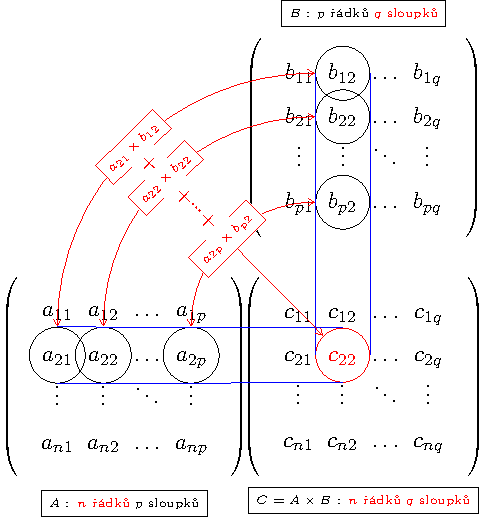
\includegraphics[width=0.45\linewidth]{mai_fig023a}}               &
        \subfloat[2. krok]{\label{LA:fig_LA001b}
          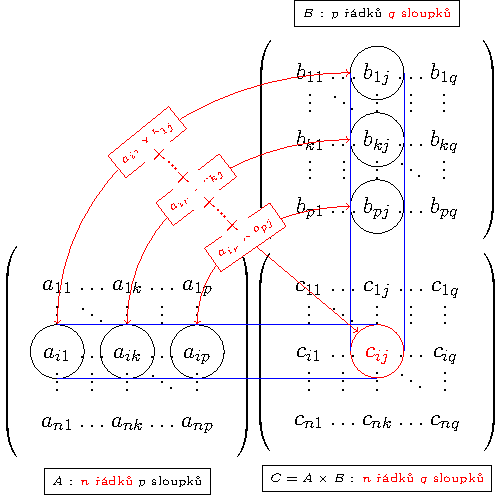
\includegraphics[width=0.45\linewidth]{mai_fig023b}} 
      \end{tabular}
      \caption{Postup při maticovém násobení}
    \end{figure}
  

      
      \begin{definition}\label{rovnost_matic}
       (Rovnost matic):  Matice \(\matr{A} = \left(a_{ij}\right)\) je rovna matici \(\matr{B}=
       \left(b_{kl}\right)\), jsou-li matice stejného typu a stejnolehlé prvky se sobě
       \textbf{rovnají}, tj. \(\matr{A} \in \mathbb{R}_{m,n}, \matr{B}\in\mathbb{R}_{m,n}, 
       a_{ij} = b_{ij}, \forall i\in\lbrace1,2,\ldots,m\rbrace, \forall j\in\lbrace1,2, \ldots 
       ,n\rbrace\).
      \end{definition}
      
%--------------------------------------------------------------------------------------------------
  \section{Počítání s vektory}\label{mai:IchapIIsecIV}
    \textbf{Vektory} budeme nazývat matice typu \(1/n\) a značit je
    \begin{equation*}
      \vec{u} = (u_1, u_2, \ldots, u_n).
    \end{equation*}
    Takže počítat s nimi již umíme! (V zápisu složek vektoru je vynechán řádkový index. V případě 
    matice s jedním řádkem, takzvané \emph{řádkové matice}, je totiž zbytečný.) Číslům \(u_1\) až 
    \(u_n\) budeme pro tuto chvíli říkat \emph{složky vektoru} \(\vec{u}\). Za chvíli tento pojem 
    ještě upřesníme. Celou řadu pojmů, s nimiž jsme se seznámili při počítání s maticemi, můžeme 
    pro vektory přímo použít. Namísto značení \(\mathcal{M} (1/n)\) budeme pro prostor vektorů 
    používat symbol \((\mathbb{R}^n)\) nebo \(\mathbb{C}^n\) (obvyklý symbol pro množinu 
    uspořádaných \(n\)-tic reálných nebo komplexních čísel).
    
    \subsection{Součiny vektorů}
      Kromě základních operací s vektory, tj. sčítání vektorů a násobení vektoru skalárem, se 
      často používají další operace, které obohacují \emph{strukturu vektorového prostoru}. 
      Zůstaneme u vektorů v trojrozměrném prostoru \(\mathbb{R}^3\) a definujeme si skalární, 
      vektorový a smíšený součin vektorů. Skalární součin vektorů definujeme prostřednictvím 
      geometrické definice jako zobrazení, které uspořádané dvojici vektorů (volných vektorů nebo 
      jejich libovolných umístění) přiřazuje reálný číslo podle předpisu
      \begin{equation}\label{mai:eq038}
        \vec{u}\vec{v} = \abs{\vec{u}}\cdot\abs{\vec{v}}\cos\varphi,
      \end{equation}
      kde \(\varphi = \sphericalangle(\vec{u},\vec{v})\) je velikost minimálního z obou úhlů mezi 
      vektory\(\vec{u},\vec{v}\).

    %---------------------------------------------------------------
    % !TeX spellcheck = cs_CZ
% \wikitextrule
\begin{mdframed}[style=mdexam]
  \begin{example}\label{mai:exam034}
    Vypočteme z definice \ref{mai:eq038} skalární součiny vektorů ortonormální báze \(\vec{e_1}\), 
    \(\vec{e_2}\) a \(\vec{e_3}\), spjaté s kartézskou soustavou souřadnic. Připomeňme, že tyto 
    vektory jsou jednotkové a navzájem kolmé.
    \begin{itemize}
      \item pro \(i\neq j\) \(\vec{e_i}\vec{e_j}=0\), 
                \(\sphericalangle\vec{e_i}\vec{e_j} =\dfrac{\pi}{2}\), vektory jsou kolmé,
      \item pro \(i = j\) \(\vec{e_i}\vec{e_j}=0\), 
                \(\sphericalangle\vec{e_i}\vec{e_j} =0, \abs{\vec{e_i}}=1\), vektory jsou 
                jednotkové.
    \end{itemize}

    Pro skalární součiny vektorů ortonormální báze použijeme zkrácené značení
    \begin{equation}\label{mai:eq085}
      \vec{e_i}\vec{e_j} = \delta_{ij},
    \end{equation}
    kde \(\delta_{ij}\) nabývá hodnoty \num{1} pro \(i = j\) a hodnoty \num{0} pro \(i \neq j\). 
    Nazývá se \textbf{Kroneckerovo delta} \cite[s.~40]{Musilova2009MA1}.
  \end{example}
\end{mdframed}
    %---------------------------------------------------------------
    
    Shrneme nyní vlastnosti skalárního součinu. Dokázat bychom je mohli, i když by to mohlo být i 
    velmi pracné, užitím znalostí z goniometrie. Zkuste to alespoň pro jednu z nich! Třeba se    
    vám podaří zvolit si tu nejjednodušší.

%} % tikzset
%---------------------------------------------------------------------------------------------------
\printbibliography[title={Seznam literatury}, heading=subbibliography]
\addcontentsline{toc}{section}{Seznam literatury}
%  % !TeX spellcheck = cs_CZ
% Differential calculus
%{\tikzset{external/prefix={tikz/MAI/}}
% \tikzset{external/figure name/.add={ch03_}{}}
%---------------------------------------------------------------------------------------------------
% Limits_of_Functions.tex
%---------------------------------------------------------------------------------------------------
\chapter{Limita a spojitost funkce}\label{mai:IchapLimit}
\minitoc

  %================Podkapitola: Reálná funkce ======================================================
  \section{Reálná funkce}
    %-----------------------------------------------------------------------------------------------
    \small
    S funkcemi se setkáváme na každém kroku nejen ve fyzice a v ostatních přírodních vědách, ale i 
    v každodenním životě. Každá situace, kdy jsou nějaký jev či veličina jednoznačně a nevyhnutelně 
    určeny jinými jevy či veličinami, se dá popsat pomocí funkce\footnote{V matematice abstrahujeme 
    při zkoumání funkcionálních závislostí od konkrétní fyzikální povahy proměnných veličin a 
    chápeme je jako \uv{bezrozměrné veličiny}, tedy jako číselné proměnné. Někdy je jednoduché 
    takovou} funkci sestavit. Snadno například můžeme zjistit, jakou dráhu urazí automobil jedoucí 
    známou rychlostí v závislosti na tom, jak dlouho jede. Nebo dokážeme určit přírůstek našich 
    úspor ve spořitelně v závislosti na době spoření, pokud známe úrokovou míru a její změny. Jindy 
    je naopak skoro nemožné přijít na to, jak taková funkce vypadá, neboť nemáme dostatek informací 
    o parametrech, které do jejího zápisu vstupují. Třeba takovou závislost teploty ovzduší v daném 
    okamžiku na zeměpisné poloze a nadmořské výšce, kterou bychom si mohli představit jako jednu ze 
    samozřejmých součástí předpovědi počasí, bychom asi nesestavili. Popis jevů pomocí funkcí je v 
    každém případě velmi užitečný. Má však svá pravidla, s nimiž se v této kapitole seznámíme. 
    Závisí-li zkoumaný jev nebo veličina na jediné veličině, jejíž hodnoty jsou reálné a buď se 
    mění známým způsobem, nebo si je můžeme dokonce volit, hovoříme o \textbf{funkci jedné reálné 
    proměnné}. A lze-li zkoumaný jev nebo veličinu kvantifikovat rovněž pomocí reálných hodnot, 
    jedná se o \textbf{reálnou funkci jedné reálné proměnné}. Právě o takových funkcích bude v této 
    kapitole řeč. V aplikacích se budeme věnovat především funkcím, které mají význam ve fyzice a v 
    přírodních vědách. Velmi často půjde o funkce, kde reálnou proměnnou je čas. Jevy v přírodě 
    podléhají totiž principu příčinnosti, a tak lze velké množství veličin popisujících přírodní 
    jevy vyjádřit na základě znalosti přírodních zákonů jako funkce času. 
    \cite[s.~53]{Musilova2009MA1}
    \normalsize
    \subsection{Funkce a její graf}\label{MAI:section_002}
      V tomto odstavci se naučíme funkce zadávat, počítat s nimi a vyjádřit je velmi přehledným 
      způsobem — jejich \emph{grafem}. Zopakujme, že každou \textbf{reálnou funkci}, jejíž 
      definiční obor je podmnožina množiny \(\realset\), nazýváme \textbf{reálnou funkcí jedné 
      reálné proměnné}\footnote{Místo názvu \uv{reálná funkce jedné reálné proměnné} budeme pro 
      stručnost používat pouze název \uv{funkce}, pokud nebude řečeno něco jiného}.
      
      Protože \emph{funkce je speciální případ zobrazení}, můžeme všech\-ny pojmy a obecné 
      vlastnosti zobrazení přenést i na funkce. Některé z nich však vzhledem k důležitosti 
      zopakujme, případně doplníme. Na druhé straně budeme studovat také ty vlastnosti, které jsou 
      specifické pro tento speciální druh zobrazení.
      
      \begin{note}
        Je-li \(\mathcal{D}_f = \naturalset\), jedná se o \textbf{posloupnost}. (Speciálním 
        případem reálných funkcí jedné reálné proměnné jsou \emph{posloupnosti reálných čísel)}.
      \end{note}
      
      \subsection{Způsoby zadání funkce}\label{MAI:section_000}
        Nejprve funkci definujeme. Předpokládejme, že reálná proměnná, na níž bude záviset náš jev, 
        má dovoleno nabývat hodnot z určité předem stanovené podmnožiny \(D\subseteq\realset\) 
        reálných čísel. Předpokládejme dále, že podle určitého pravidla, předpisu, dokážeme pro 
        \emph{každou hodnotu} \(x\) množiny \(\mathcal{D}_f\), tj. \(x \in \mathcal{D}_f\), určit 
        \emph{právě jednu} reálnou hodnotu \(y\). Každé hodnotě \(x \in D\) tedy nějaké \(y\) 
        příslušet \emph{musí},  avšak žádné hodnotě \(x\) \emph{nesmíme} přiřadit více hodnot 
        \(y\). Tak vzniká funkce \(f\). Hodnoty \(x\) se nazývají hodnotami \emph{nezávisle 
        proměnné} (neboli \emph{argumentu}), hodnoty \(y\) hodnotami \emph{závisle proměnné} a 
        \(f\) symbolizuje \emph{funkční předpis}. Píšeme
        \begin{equation}\label{mai:eq000}
            f: x \in \mathcal{D}_f \rightarrow y=f(x)\in\realset
        \end{equation}
      Hodnoty proměnné \(x\) nazýváme též \emph{vzory}, odpovídající hodnoty \(y = f(x)\) 
      \emph{obrazy}. Množina  \(\mathcal{D}_f\) je \emph{definičním oborem} funkce \(f\). Zadání 
      definičního oboru je důležitou součástí zadání funkce. Množina \(H\) všech takových reálných 
      hodnot \(y\), které jsou obrazem nějakého vzoru, 
      \begin{equation}\label{mai:eq001}
          \mathcal{H}_f = 
              \left\lbrace 
                y\in\realset\text{ existuje } x\in \mathcal{D}_f, \text{ tak že } y = f(x)  
              \right\rbrace, 
      \end{equation}
      se nazývá \emph{obor hodnot} funkce \(f\). Hodnotu \(f(x)\) nazýváme také \emph{funkční 
      hodnotou} funkce \(f\) v bodě \(x\). 

      \begin{figure}[ht!] %\ref{mai:fig001}
        \centering
%        % Funkce jako „černá skříňka“. \cite[s.~54]{Musilova2009MA1}

\documentclass[11pt]{standalone}
\usepackage{xltxtra}
\usepackage{tikz}
\usepackage{amsmath}

\begin{document}
  \begin{tikzpicture}[fill=black!20]
%  \draw[help lines] (-1,-2) grid (6,3);
    \path (0,0) node(a) [ ] {\(\mathcal{D}_f\)}
    (2,0) node(b) [rectangle,rotate=0,draw,fill] {\(\begin{array}{c} \text{funkce} \\ f(x)  
    \end{array}\)}
    (4,0) node(c) [ ] {\(\mathcal{H}_f\)};
    \draw[thick,->] (a.east) -- (b);
    \draw[thick,->] (b.east) -- (c);
    \path [ ] (a.east) -- (b.west)   node [above,midway] {\(x\)};
    \path [ ] (b.east) -- (c.west)   node [above,midway] {\(y\)};
  \end{tikzpicture}

\end{document}
        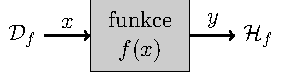
\includegraphics[width=0.45\linewidth]{mai_fig001.pdf}
        \caption{Funkce jako „černá skříňka“. \cite[s.~54]{Musilova2009MA1}}
        \label{mai:fig001}
      \end{figure}
      
      Funkci si podle obrázku \ref{mai:fig001} můžeme představit jako „černou skříňku“, do které 
      vstoupí hodnota (vzor) a vystoupí z ní hodnota \(y = f(x)\) (obraz). Množinu uspořádaných 
      dvojic čísel \([x, f(x)]\) nazveme \hyperref[MAI:section_001]{grafem funkce}.
      
      Jak zadat předpis \(f\)? Lze to udělat kterýmkoli z následujících způsobů, podle vhodnosti
      nebo snadnosti. Ukážeme jednotlivé možnosti na jednoduchém příkladu, kdy chceme hodnotám 
      proměnné \(x\) z množiny \(\mathcal{D}_f\) přiřadit jejich druhé mocniny. Zvolme pro náš 
      příklad definiční obor výčtem:
      \begin{equation*}
         \mathcal{D}_f = \lbrace-3,2,-1,0,1,2,3,4\rbrace,
      \end{equation*}
      a zadáme předpis
      \begin{itemize}\addtolength{\itemsep}{-0.5\baselineskip}
        \item \textbf{slovním popisem}: předpis \(f\) přiřazuje každé z hodnot \(x\in 
              \mathcal{D}_f\) její druhou mocninu,
        \item \textbf{vzorcem}: \(y = x^2\) pro \(x\in \mathcal{D}_f\) zadává zobrazení
              \begin{equation*}
                f: x\in \mathcal{D}_f \rightarrow f(x)= x^2\in\realset,
              \end{equation*}
        \item \textbf{tabulkou}: Hodnoty obrazů pro všechny vzory z \(\mathcal{D}_f\) vypíšeme do 
              tabulky:
              \begin{table}[h]
                \centering
                \begin{tabular}{c|rrrrrrrr}
                  \textbf{x} & -3 & -2 & -1 & 0 & 1 & 2 & 3 & 4  \\ \hline
                  \textbf{y} & 9  & 4  & 1  & 0 & 1 & 4 & 9 & 16
                \end{tabular}
                % \caption{ }
              \end{table}
              Proměnná $x$ se v tomto případě mění \uv{diskrétně}. Je zřejmé, že tímto způsobem 
              můžeme funkci definovat úplně jen tehdy, je-li definiční obor konečná množina. 
              Tabulku však používáme i v jiných případech, zejména chceme-li vyznačit pomocí ní, 
              některé hodnoty, které nás z nějakého důvodu přednostně zajímají. 
        \item Zadání \textbf{grafem}: 
          \begin{equation*}
            G_f = \left\lbrace\left[x,f(x)\right] |x\in D\right\rbrace
                = \left\lbrace\left[x,x^2 \right] |x\in D\right\rbrace
          \end{equation*}
          tak, že dvojice \([x, f(x)]\) znázorníme jako body v rovině (obr. \ref{MAI:fig_011}).
          \begin{figure}[ht!]
            \centering  
            \begin{tabular}{cc}
              \subfloat[ ]{\label{MAI:fig_011}
                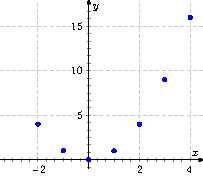
\includegraphics[width=0.4\linewidth]{mai_fig002.pdf}}              &
              \subfloat[ ]{\label{MAI:fig_010}
                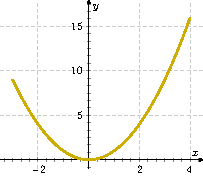
\includegraphics[width=0.4\linewidth]{mai_fig003.pdf}}              \\
            \end{tabular}
            \caption{Zadání funkce grafem}
          \end{figure}
          Z grafu můžeme ovšem funkční hodnoty určit pouze přibližně. Pro další matematické 
          zpracování je grafické zadání nejméně vhodné, i když jeho praktický význam například v 
          technických aplikacích nelze popřít.
        \item Zadání pomocí \textbf{rovnice}, jíž je funkce řešením: některé funkce nelze jednoduše 
              zapsat pomocí některého z předchozích způsobů, nebo to alespoň nejde přesně. Lze však 
              zapsat (diferenciální) rovnici, kterou tato funkce splňuje. Jedná se většinou o 
              speciální funkce, jimž se v tomto textu nebudeme věnovat. (Někdy může být taková 
              rovnice  představující zadání funkce i velmi jednoduchá. Například dosti známá funkce 
              \(\erf(x)\), \emph{error funkce}, velmi úzce souvisí s funkcí \(f(x) = 
              \frac{2}{\sqrt{x}}e^{-x^2}\). Nelze ji však zapsat vzorcem. Některé její hodnoty v 
              nejčastěji používaném rozsahu proměnné \(x\) můžeme najít v rozsáhlých tabulkách, 
              které byly sestaveny pomocí numerických metod.)
      \end{itemize}
      
      Již bylo zmíněno, že zadání definičního oboru je neopominutelnou součástí zadání funkce. 
      Kdybychom například zadali funkci opět předpisem \(y=x^2\), avšak za definiční obor stanovili 
      uzavřený interval \(D = \lbrace —3,4\rbrace\), dostali bychom graf na obrázku 
      \ref{MAI:fig_010}. Jde skutečně o jinou funkci než na obrázku \ref{MAI:fig_011}. Její úplnou 
      tabulku bychom nedokázali napsat vůbec.
      
%      Nejčastější způsob zadání funkce představuje \emph{vzorec}. Tabulku alespoň pro některé 
%      hodnoty z \(\mathcal{D}_f\) si pak dokážeme sestavit a schematický graf nakreslit. Někdy se 
%      objeví zadání funkce jen v podobě vzorce, například: „Je dána funkce \(y = f(x)\).“ Znamená 
%      to, že autor zapomněl zadat definiční obor? Nemusí tomu tak být. Tento způsob zadání chápeme 
%      tak, že si sami musíme stanovit „co největší“ definiční obor této funkce, tj. určit množinu 
%      všech takových \(x\), pro která lze do vzorce dosadit a hodnotu \(y\) určit.

      Zobrazovací předpis, kterým je funkce zadána, může být rozmanitý. Nejčastěji a pro účely 
      matematické analýzy nejvhodnější je \emph{analytické zadání vzorcem}, tj. rovnicí tvaru 
      $y=f(x)$ nebo několika takovými rovnicemi platnými pro různé části definičního oboru. Přitom 
      v rovnici $y=f(x)$ je na pravé straně nějaký správně definovaný výraz obsahující nejvýše 
      proměnnou $x$ a nabývající jednoznačné hodnoty pro danou hodnotu proměnné $x$.
      
%      Někdy však používáme (poněkud nedůsledně) termíny \uv{funkce \(f(x)\)} nebo \uv{funkce 
%      \(y=f(x)\)}. V tomto smyslu nepojímáme již \(x\) jako pevný prvek z definičního oboru, ale 
%      jako \uv{nezávisle proměnnou} neboli \emph{argument}, tj. symbol zastupující libovolný prvek 
%      z definičního oboru. V tomto případě pak písmeno \(y\) v rovnici \(y=f(x)\) nazýváme 
%      \emph{závisle proměnnou} a říkáme, že \uv{\(y\) závisí na \(x\)}. Tato frazeologie má své 
%      historické kořeny; tento způsob vyjádření funkce budeme využívat zřídka, zejména tam, kde 
%      nechceme pro označení příslušné funkce zavádět zvláštní symbol. Tak např. budeme mluvit o 
%      funkci \(e^x\) (ačkoliv se zavádí pro exponenciální funkci symbol exp) nebo o funkci \(\sin 
%      x\) (ačkoliv by bylo důslednější mluvit o funkci \(\sin\)) apod. \cite[s.~82]{Brabec1989} 

    %-------------------------------------
      % !TeX spellcheck = cs_CZ
\begin{mdframed}[style=mdexam]
  \begin{example}\label{MAI:exam017}
    (Definiční obor a obor hodnot funkce): Určíme „co největší“ definiční obor funkce
    \(y=\log_2{(\sqrt{1-x^2})}\) a zjistíme také její obor hodnot.
        
    {\centering
    \captionsetup{type=figure}
  %   % !TeX spellcheck = cs_CZ
% exam017.tex
% K příkladu \ref{fyz:fey_exam017} \(y=\log_2{(\sqrt{1-x^2})}\) 

\documentclass[11pt]{standalone}
\usepackage{xltxtra}
\usepackage[usenames,x11names]{xcolor}
\usepackage{tikz}
\usepackage{pgfplots}
  \pgfplotsset{compat=newest}
\usepackage{amsmath}

\begin{document}
  \begin{tikzpicture}[thick,scale=0.7, every node/.style={transform shape}]
    \begin{axis}[
      xmin = -1, xmax = 1, ymin = -10, ymax = 0,
      domain = -0.999999:0.999999,
      restrict y to domain=-30:0,
      grid = major,   % both
      grid style={line width=.1pt, draw=gray!20},
      major grid style={dashed, line width=.2pt, draw=gray!40},
      minor tick num=5,
      clip = true,
      clip mode=individual,
      axis x line = middle,
      axis y line = middle,
      xlabel={\(x\)},
    %  xlabel style={at=(current axis.right of origin), anchor=west},
      ylabel={\(y\)},
    %  ylabel style={at=(current axis.above origin), anchor=south},
      enlarge y limits={rel=0.13},
      enlarge x limits={rel=0.07},
    ]
    
     \addplot[color=Gold3, samples=1000, smooth, ultra thick, unbounded coords=jump, no markers] 
        gnuplot{log10(sqrt(1-x^2))/log10(2)};  
    \end{axis}
  \end{tikzpicture}

\end{document}

% note: předchozí varianta MAI013
%\begin{tikzpicture}
%    \begin{axis}[
%        axis lines=middle,
%        width=10cm, height=10cm,     % size of the image
%        grid = both,
%        grid style={dashed, gray!30},
%        enlargelimits=true,
%        xmin=-1,      % start the diagram at this x-coordinate
%        xmax= 1,      % end   the diagram at this x-coordinate
%        ymin= -6,     % start the diagram at this y-coordinate
%        ymax= 0.5,     % end   the diagram at this y-coordinate
%        /pgfplots/xtick={-1,-0.5,...,1},   % make steps of length 0.2
%        /pgfplots/ytick={0,-0.5,...,-6},   % make steps of length 0.1
%        axis background/.style={fill=white},
%        axis line style={thick, shorten >=2pt, ->, > = {Latex[scale=1.3]}},
% %       every axis x label/.style={
% %        at={(ticklabel* cs:1.0)},
% %        anchor=west,
% %       },
% %       every axis y label/.style={
% %        at={(ticklabel* cs:1.0)},
% %        anchor=south,
% %       },
%        every axis x label/.style={at={(current axis.right of origin)},anchor=west},
%        every axis y label/.style={at={(current axis.north)},above=0mm},
%        ylabel=\(y\),
%        xlabel=\(x\),
% %       title={Dirichletova funkce}
%      ]
%      \addplot[domain=-0.9999:0.9999, line width=0.5pt,samples=1000,red]{log2(sqrt(1-x^2))};
%    \end{axis} 
%\end{tikzpicture}
    \luafigure[0.9]{mai_fig004.pdf}
    \captionof{figure}{K příkladu \ref{MAI:exam017} \(y=\log_2{(\sqrt{1-x^2})}\) 
    \cite[s.~57]{Musilova2009MA1}
    \label{mai:fig004}}
    \par}
    
    Využijeme našich znalostí ze střední školy. Ve hře jsou tři funkce: logaritmus, odmocnina a
    kvadratická funkce, postupně: 
    \begin{equation*}
      y = \log_2w, \qquad w = \sqrt{u}, \qquad u = 1 - x^2.
    \end{equation*}
    „Největším“ definičním oborem logaritmu je množina \(\mathcal{D}(log) = {w\realset \mid w >
    0}\). Oborem hodnot logaritmu pro \(w \in \mathcal{D}(log)\) je celá reálná osa. Hodnoty \(w\)
    však dostáváme vyčíslením odmocniny, která pro přípustné hodnoty \(u\), \(\mathcal{D}(\sqrt{ })
    = \lbrace u\in\realset \lvert u\geq 0\rbrace\), může nabývat všech nezáporných hodnot, tj.
    kladných a hodnoty nula (té nabývá pro \(u = 0\)). Hodnotu \(w = 0\) však nesmíme do logaritmu
    dosadit, takže hodnotu \(u = 0\) musíme ihned vyloučit. Hodnoty proměnné \(x\) musíme omezit
    tak, aby kvadratická funkce \(u = 1 - x^2\) nabývala pouze kladných hodnot. Dostáváme tak
    definiční obor funkce \(y = f(x)\) \(\mathcal{D}=\lbrace x\in\realset \lvert -1<x<1\rbrace\),
    neboli otevřený interval \((-1, 1)\). Pro \(x \in \mathcal{D}\) pak funkce \(u(x)\) nabývá
    hodnot v intervalu \(\mathcal{H}_u = \left( 0, 1\right]\) a funkce \(\log_2\sqrt{1-x^2}\) hodnot
    v intervalu \(\mathcal{H}_u = \left( -\infty, 0\right]\), který je tedy jejím oborem hodnot.
    Graf funkce vidíme na obr. \ref{mai:fig004}. 
  \end{example}
\end{mdframed}
    %-----------------------------------------------------------------------------------------------
    \subsection{Graf funkce}\label{MAI:section_001}\hypertarget{MAI:section_001}
      Jinými slovy, v předchozím odstavci, bylo řečeno, že každé funkci můžeme přiřadit její graf, 
      a že \textbf{grafem funkce} $f:A\rightarrow\realset,\ A\subset\realset$, rozumíme množinu 
      všech bodů euklidovské roviny, jejíž souřadnice $x$, $y$ v dané kartézské soustavě souřadnic 
      vyhovuje rovnice 
      \begin{equation}\label{mai:eq026}
        y=f(x). 
      \end{equation}  
      
      Graf funkce může v jednodušších případech posloužit jako prostředek k získání názorné 
      \uv{představy}. Grafy některých funkcí jsou \uv{křivky}, (intuitivním smyslu tohoto slova). 
      Avšak u některých funkcí názorná představa grafu selhává. Vezmeme-li např. Dirichletovu 
      funkci, snadno zjistíme, že její graf nemůžeme sestrojit (obr. \ref{mai:fig005} tedy 
      není grafem funkce, ale pouze pokusem o názorné přiblížení Dirichletovi funkce)
      
      \begin{figure}[ht!] %\ref{mai:fig005}
        \centering
%       % !TeX spellcheck = cs_CZ
%
% Pokus o zobrazení Dirichletovy funkce: \uv{dvě rovnoběžné přímky $y=0$ a $y=1$ s 
% nekonečným množstvím mezer}
% xelatex -enable-write18 -shell-escape mai_fig005.tex

\documentclass[11pt]{standalone}
\usepackage{xltxtra}
\usepackage[usenames,x11names]{xcolor}
\usepackage{tikz}
\usepackage{pgfplots}
  \pgfplotsset{compat=newest}
\usepackage{amsmath}
\usepackage{amsfonts}           % \mathbb{Q}
\usepackage{tabularx}           % \shortstack

\begin{document}
  \begin{tikzpicture}[thick,scale=0.7, every node/.style={transform shape}]
    \begin{axis}[
      xmin = -3, xmax = 3, ymin = 0, ymax = 2,  % osy
      domain = -3:3,
      restrict y to domain=0:4,
      grid = major,   % both
      grid style={line width=.1pt, draw=gray!20},
      major grid style={dashed, line width=.2pt, draw=gray!40},
      minor tick num=5,
      clip = true,
      clip mode=individual,
      axis x line = middle,
      axis y line = middle,
      xlabel={\(x\)},
    %  xlabel style={at=(current axis.right of origin), anchor=west},
      ylabel={\(y\)},
    %  ylabel style={at=(current axis.above origin), anchor=south},
      enlarge y limits={rel=0.13},
      enlarge x limits={rel=0.07},
    %  title={Dirichletova funkce}
    ]
        
        \addplot[domain=-3:3, ultra thick,samples=10,blue] {1};
        \label{plot one}
        \addplot[domain=-3:3, ultra thick,samples=10,red] {0};
        \label{plot two} 
        \node [draw,fill=white] at (rel axis cs: 0.6,0.7) {\shortstack[l]{
        \(f(x) = 
          \left\lbrace\begin{array}{l@{}l@{}}
              1 & \text{ když } x \in  \mathbb{Q}\\
              0 & \text{ když } x \in  \mathbb{R} \setminus\mathbb{Q}
          \end{array}\right.
       \)
          }
           };
      \end{axis} 
  \end{tikzpicture}
\end{document}
        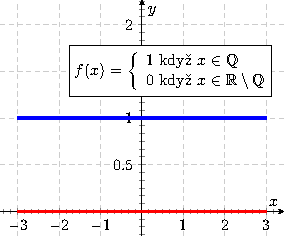
\includegraphics[width=0.5\linewidth]{mai_fig005.pdf}
        \caption{Pokus o zobrazení Dirichletovy funkce: \uv{dvě rovnoběžné přímky $y=0$ a $y=1$ s 
        nekonečným množstvím mezer}}
        \label{mai:fig005}
      \end{figure}      
      Z předchozí kapitoly také víme, že zadat funkci znamená udat její definiční obor a 
      \uv{zobrazovací předpis}, tj pravidlo (formulované slovně či v používaném matematickém 
      jazyku), podle něhož můžeme jednoznačným způsobem rozhodnout, jaká funkční hodnota odpovídá 
      libovolně zvolenému číslu z definičního oboru. Definičním oborem bývá často interval nebo 
      sjednocení intervalů. Není-li definiční obor udán, rozumíme jím množinu všech reálných čísel, 
      pro něž je příslušný předpis definován. Tuto množinu nazýváme \textbf{přirozeným} (též 
      maximálním) definičním oborem funkce. Je to tzv. \emph{existenční obor} výrazu, jímž je 
      funkce definována \cite[s.~84]{Brabec1989}.
      
      Například funkce $f: \realset\rightarrow\realset,\ f(x)=x^2$, můžeme vyjádřit bez udání 
      definičního oboru $\realset$ vztahem 
      \begin{equation*}
        f: y=x^2,
      \end{equation*}
      neboť předpis $y=x^2$ má smysl pro každé reálné číslo $x$. Avšak u funkce $g:\langle0, 
      1\rangle\rightarrow\realset,\ g(x)=x^2,$ je nutné v zápisu funkce definiční obor $\langle0, 
      1\rangle$ 
      uvést, píšeme tedy   
      \begin{equation*}
        g: y=x^2, \quad x\in\langle0,1\rangle.
      \end{equation*}
       
      %-------------------------------------
        % !TeX spellcheck = cs_CZ
\wikitextrule
\begin{example}\label{MAI:exam018} 
  Vzorcem $f(x)=\sqrt{1-x}$ je dána funkce, jejímž přirozeným oborem je interval 
  $(-\infty,1\rangle$ (uvažme, že výraz $\sqrt{1-x}$ je definován v reálném oboru, je-li 
  $1-x\geq0$). Graf této funkce je část paraboly, jejíž osou je osa $x$, viz obr. 
  \ref{mai:fig006}.
  
  {\centering
   \captionsetup{type=figure}
%  % !TeX spellcheck = cs_CZ
% mai_fig006.tex

\documentclass[11pt]{standalone}
\usepackage{xltxtra}
\usepackage[usenames,x11names]{xcolor}
\usepackage{tikz}
\usepackage{pgfplots}
  \pgfplotsset{compat=newest}
\usepackage{amsmath}


\begin{document}
  \begin{tikzpicture}[thick,scale=0.7, every node/.style={transform shape}]
    \begin{axis}[
      xmin = -3, xmax = 1.5, ymin = 0, ymax = 3,  % osy
      domain = -3:1,
      restrict y to domain=0:4,
      grid = major,   % both
      grid style={line width=.1pt, draw=gray!20},
      major grid style={dashed, line width=.2pt, draw=gray!40},
      minor tick num=5,
      clip = true,
      clip mode=individual,
      axis x line = middle,
      axis y line = middle,
      xlabel={\(x\)},
    %  xlabel style={at=(current axis.right of origin), anchor=west},
      ylabel={\(y\)},
    %  ylabel style={at=(current axis.above origin), anchor=south},
      enlarge y limits={rel=0.13},
      enlarge x limits={rel=0.07},
    ]
    
     \addplot[color=Gold3, samples=200, smooth, ultra thick, unbounded coords=jump, no markers] 
        gnuplot{sqrt(1-x)};  
    \end{axis}
  \end{tikzpicture}
\end{document} 
   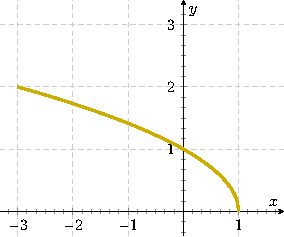
\includegraphics[width=0.5\linewidth]{mai_fig006.pdf}
   \captionof{figure}{{Graf funkce $y=\sqrt{1-x}$ je část paraboly, jejíž hlavní osou je osa $x$}}
   \label{mai:fig006}
   \par}

\end{example}
      %-------------------------------------
      
      %-------------------------------------
        % !TeX spellcheck = cs_CZ
\begin{mdframed}[style=mdexam]
  \begin{example}\label{MAI:exam019} 
    Funkce je dána vzorcem 
    \begin{equation*}
      f(x):y=\abs{x}.
    \end{equation*} 
    Přirozeným definičním oborem této funkce je množina $\realset$. Táž funkce může být dána i 
    vzorcem
    \begin{equation*}
      f(x):y=\sqrt{x^2},
    \end{equation*}    
    nebo dvěma rovnicemi
    \begin{equation*}
      f(x):y=
        \begin{cases}
             x & \text{je-li} x \geq 0. \\
            -x & \text{je-li} x < 0,
        \end{cases}                 
    \end{equation*}  
    což je zřejmé, uvědomíme-li si jak je definována absolutní hodnota. Graf funkce je na obr. 
    \ref{mai:fig007}.
    
    {\centering
    \captionsetup{type=figure}
  %  % !TeX spellcheck = cs_CZ
% mai_fig007.tex

\documentclass[11pt]{standalone}
\usepackage{xltxtra}
\usepackage[usenames,x11names]{xcolor}
\usepackage{tikz}
\usepackage{pgfplots}
  \pgfplotsset{compat=newest}
\usepackage{amsmath}

\begin{document}
  \begin{tikzpicture}[thick,scale=0.7, every node/.style={transform shape}]
    \begin{axis}[
      xmin = -3, xmax = 3, ymin = 0, ymax = 3,  % osy
      domain = -3:3,
      restrict y to domain=0:3,
      grid = major,   % both
      grid style={line width=.1pt, draw=gray!20},
      major grid style={dashed, line width=.2pt, draw=gray!40},
      minor tick num=5,
      clip = true,
      clip mode=individual,
      axis x line = middle,
      axis y line = middle,
      xlabel={\(x\)},
    %  xlabel style={at=(current axis.right of origin), anchor=west},
      ylabel={\(y\)},
    %  ylabel style={at=(current axis.above origin), anchor=south},
      enlarge y limits={rel=0.13},
      enlarge x limits={rel=0.07},
    ]
    
     \addplot[color=Gold3, samples=200, smooth, ultra thick, unbounded coords=jump, no markers] 
        gnuplot{abs(x)};  
    \end{axis}
  \end{tikzpicture} 
\end{document}
    \luafigure[0.9]{mai_fig007.pdf}
    \captionof{figure}{Graf funkce $y=\abs{x}$}
    \label{mai:fig007}
    \par}
  \end{example}
\end{mdframed}
      %-------------------------------------
      
      Funkce může být analyticky zadána i jinak než vzorcem $y=f(x)$. Časté je \textbf{parametrické 
      vyjadřování}, tj. vyjádření dvojicí rovnic 
      \begin{equation}\label{mai:eq027}
        x=\varphi(t),\ y=\psi(t),\ t\in J,
      \end{equation}
      kde $\varphi, \psi$ jsou funkce definované na množině $J$ ($\ J$ bývá obvykle interval). 
      Proměnná $t$ se nazývá \emph{parametr}: má zde pomocný význam. Zajímá nás totiž vztah mezi 
      $x$ a $y$. Rovnice \ref{mai:eq027} definuje relaci 
      $f\subset\realset\times\realset=\realset^2$:
      \begin{equation*}
        f = \{(x,y)\in\realset^2; \text{ existuje } t\in J \text{ tak, že } x=\varphi(t),\ y=\psi(t)\}.
      \end{equation*}      
      Tato relace může být za \emph{určitých podmínek jednoznačná} tj. je funkcí z $\realset$ do 
      $\realset$. V tomto případě říkáme, že funkce $f$ je \emph{definována parametricky rovnicemi 
      \ref{mai:eq027}}
      
      %-------------------------------------
        % !TeX spellcheck = cs_CZ
\begin{mdframed}[style=mdexam]
  \begin{example}\label{mai:exam020} 
    Rovnice $x=\cos t,\ y=\sin t\quad t\in\langle0,\pi\rangle$, definují parametricky funkci 
    \begin{equation}
      f: y= \sqrt{1-x^2}, \quad x\in\langle-1,1\rangle,
    \end{equation}
    jejíž grafem je polokružnice, ležící v horní polorovině $\{(x,y)\in\realset^2, y\geq0\}$.
    
    {\centering
    \captionsetup{type=figure}
  %   % !TeX spellcheck = cs_CZ
%Graf funkce \(y=\sqrt{1-x^2}\) je polokružnice

\documentclass[11pt]{standalone}
\usepackage{xltxtra}
\usepackage[usenames,x11names]{xcolor}
\usepackage{tikz}
\usepackage{pgfplots}
  \pgfplotsset{compat=newest}
\usepackage{amsmath}

\begin{document}
  \begin{tikzpicture}[thick,scale=0.7, every node/.style={transform shape}]
    \begin{axis}[
      xmin = -1.2, xmax = 1.2, ymin = 0, ymax = 1.3,  % osy
      domain = -1:1,
      restrict y to domain=0:1,
      unit vector ratio=1 1 1,  % axis equal
      grid = major,   % both
      grid style={line width=.1pt, draw=gray!20},
      major grid style={dashed, line width=.2pt, draw=gray!40},
      minor tick num=5,
      clip = true,
      clip mode=individual,
      axis x line = middle,
      axis y line = middle,
      xlabel={\(x\)}, ylabel={\(y\)},
      enlarge y limits={rel=0.07},
      enlarge x limits={rel=0.07},
    ]
    
      \addplot[color=Gold3, samples=200, smooth, ultra thick, unbounded coords=jump, no markers] 
         gnuplot{sqrt(1-x^2)};  
    \end{axis}
  \end{tikzpicture} 
\end{document}
    \luafigure[0.9]{mai_fig008.pdf}
    \captionof{figure}{Graf funkce \(y=\sqrt{1-x^2}\) je polokružnice}
    \label{mai:fig008}
    \par}
  \end{example}
\end{mdframed}
      %-------------------------------------
      
      Blíže se parametrickým zadáním funkce budeme zabývat v kapitole \ref{chap:Apl_dif_poc}
      (Aplikace diferenciálního počtu).
      
      Funkce může být někdy zadána též rovnicí tvaru 
      \begin{equation}\label{mai:eq028}
        F(x,y) = 0.
      \end{equation}
      Přitom $F$ je funkce dvou proměnných, tj. zobrazení z $\realset^2\rightarrow\realset$. Kromě 
      rovnice \ref{mai:eq028} může být dána ještě podmínka, aby bod $(x,y)$ patřil k některé 
      množině $M\subset\realset^2$. Rovnicí \ref{mai:eq028} je definována opět jakási relace 
      $f\subset\realset\times\realset$,
      \begin{equation}
        f = \{(x,y)\in\realset^2,\quad F(x,y)=0 \}
      \end{equation}
      (případně $f = \{(x,y)\in\realset^2,\ F(x,y)=0,\ (x,y)\in M \}$), zajímá nás, kdy tato relace 
      je funkcí z $\realset$ do $\realset$. Říkáme pak, že funkce $f$ je dána \textbf{implicitně} 
      uvedenou rovnicí \ref{mai:eq028} (příp. rovnicí \ref{mai:eq028} a podmínkou $(x,y)\in 
      M$). Naproti tomu zadání funkce ve tvaru $y=f(x)$ nazýváme \textbf{explicitním}.

      %-------------------------------------
        % !TeX spellcheck = cs_CZ
\begin{mdframed}[style=mdexam]
  \begin{example}\label{MAI:exam022}\todo[inline]{Nedokončený příklad}
    \begin{itemize}
    \item[]
    \item  Rovnicí $x+2y-3=0$ je implicitně definována funkce  
          $f:y=-\dfrac{1}{2}x+\dfrac{3}{2}$.
    \item  Rovnicí $x^2+y^2=1$ a podmínkou $y\geq0$ je definována implicitní funkce z příkladu 
          \ref{MAI:exam020}. Relace $\{(x,y)\in\realset^2;\ x^2+y^2=1\}$ není ovšem jednoznačná, 
          každé hodnotě $x\in(-1,1)$ odpovídají dvě hodnoty $y: y_1=\sqrt{1-x^2}$, $y: y_2 = 
          -\sqrt{1-x^2}$. Podmínkou $y\geq0$ druhou hodnotu vylučujeme. Místo podmínky $y\geq0$ 
          bychom mohli uvést i jiné podmínky, aby rovnice $x^2+y^2=1$ určovala implicitní funkci.   
    \end{itemize}
  \end{example}
\end{mdframed}
      %-------------------------------------
      
      Vyšetřování podmínek, při nichž rovnice $F(x,y)=0$ je definována funkce $f$, se obvykle 
      provádí metodami matematické analýzy funkce více proměnných. 
          
    %---------------------------------------------------------------------------------------------- 
    \subsection{Vlastnosti funkcí}\label{MA1:subsec_vlastnosti_funkce}
      \subsubsection{Omezená funkce}
        \begin{definition}\label{MA1:def_lim01}
          Funkci $f$ nazýváme shora (zdola) omezenou na množině $A\subset D(f)$, je-li shora 
          (zdola) omezená množina funkčních hodnot $f(A)$. Je-li funkce $f$ omezená shora i zdola 
          na množině $A$, pak ji nazýváme omezenou na množině $A$. Je-li $A=D(f)$, nazýváme funkci 
          omezenou. Viz kniha \cite[s.~87]{Brabec1989}       
        \end{definition}
        Funkce \(f\) je omezená na množině \(A\), právě když existuje číslo \(K>0\) tak, že platí
        \begin{align*}
         |f(x)|      &\leq K \qquad \text{pro každé } x\in A   \\ 
         \shortintertext{neboli}
         -K\leq f(x) &\leq K \qquad \text{pro každé } x\in A. 
        \end{align*}

        %-------------------------------------
          % !TeX spellcheck = cs_CZ
\wikitextrule
\begin{example}\label{MAI:exam023}
  Funkce $f:y=\dfrac{1}{x^2+1}$ je omezená. Platí totiž 
  \begin{equation*}
    \left|\frac{1}{x^2+1}\right|=\frac{1}{x^2+1}\leq1 \qquad \text{pro všechna }x\in\realset.
  \end{equation*}
  Zdola je tato funkce omezena dokonce číslem $0$.  
\end{example}
        %-------------------------------------

        \begin{itemize}\addtolength{\itemsep}{-0.5\baselineskip}
          \item Je-li funkce $f$ shora omezená na množině $A$, existuje konečné \emph{supremum}     
                $\sup f(A)$. Toto číslo nazýváme \emph{supremem funkce $f$ na množině $A$} a 
                označujeme je též $\sup_{x\in A}f(A)$ nebo $\sup\{f(x), x\in A\}$.
          \item Je-li funkce $f$ zdola omezená na množině $A$, existuje konečné \emph{infimum} 
                $\inf(A)$, které nazýváme \emph{infimum funkce $f$ na množině $A$} a označujeme je 
                též $\inf_{x\in A}f(A)$ nebo $\inf\{f(x), x\in A\}$. 
          \item Není-li funkce $f$ shora (zdola) omezená na množině $A$, pak je ovšem $\sup_{x\in A}
                f(x)=+\infty$ ($\sup_{x\in A} f(x)=-\infty$).
          \item Má-li množina $f(A)$ největší (nejmenší) prvek, pak toto číslo nazýváme největší 
                (nejmenší hodnotou funkce $f$  na množině $A$ (je-li $A = f(f)$, též absolutním 
                maximem, resp. absolutním minimem funkce $f$) a značíme je $\max_{x\in A} f(x)$ 
                ($\min_{x\in A} f(x)$). V tomto případě existuje takové číslo $x_0\in A$, že 
                $f(x_0)=\max_{x\in A}f(x)$ ($f(x_0)=\min_{x\in A}f(x)$). Pro všechna $x\in A$ tedy 
                platí $f(x)\leq f(x_0)$ ($f(x)\geq f(x_0)$). Je zřejmé, že největší (nejmenší) 
                hodnota funkce $f$ na množině $A$, pokud existuje je současně supremem (infimem) 
                funkce $f$ na $A$.
        \end{itemize}

      %-------------------------------------
        % !TeX spellcheck = cs_CZ
\wikitextrule
\begin{example}\label{MAI:exam021} 
  Pro funkci z příkladu \ref{MAI:exam023} platí:
  \begin{align*}
    \sup_{x\in\realset}&=\frac{1}{x^2+1}=\max_{x\in\realset}=\frac{1}{x^2+1}=1;   \\
    \inf_{x\in\realset}&=\frac{1}{x^2+1}=0,
  \end{align*}
  tato funkce však nenabývá v definičním oboru $\realset$ nejmenší hodnoty, neboť je stále 
  $\dfrac{1}{x^2+1}>0$. To, že infimum je $0$, dokážeme takto: Zvolíme-li libovolně 
  $\varepsilon>0$, pak snadno zjistíme, že existuje $x$, pro něž 
  $\dfrac{1}{x^2+1}<\varepsilon$:
  \begin{align*}
    1                  &< \varepsilon(x^2+1) \\
    \frac{1}{\epsilon} &< x^2+1 \Rightarrow \sqrt{\frac{1}{\epsilon}-1} < x
  \end{align*} 
  
  {\centering
   \captionsetup{type=figure}
%   % !TeX spellcheck = cs_CZ
%Graf funkce $f(x):y=\dfrac{1}{1+x^2}$

\documentclass[11pt]{standalone}
\usepackage{xltxtra}
\usepackage[usenames,x11names]{xcolor}
\usepackage{tikz}
\usepackage{pgfplots}
  \pgfplotsset{compat=newest}
\usepackage{amsmath}

\begin{document}
  \begin{tikzpicture}[thick,scale=0.7, every node/.style={transform shape}]
    \begin{axis}[
      xmin = -4.2, xmax = 4.5, ymin = 0, ymax = 1.3,  % osy
      domain = -4:4,
      restrict y to domain=0:1,
  %    unit vector ratio=1 1 1,  % axis equal
      grid = major,   % both
      grid style={line width=.1pt, draw=gray!20},
      major grid style={dashed, line width=.2pt, draw=gray!40},
      minor tick num=5,
      clip = true,
      clip mode=individual,
  %    /pgfplots/xtick={-2,-1,1,2}, % make steps of length 0.2
      axis x line = middle,
      axis y line = middle,
      xlabel={\(x\)}, ylabel={\(y\)},
      enlarge y limits={rel=0.07},
      enlarge x limits={rel=0.07},
    ]
    
      \addplot[color=Gold3, samples=200, smooth, ultra thick, unbounded coords=jump, no markers] 
         gnuplot{1/sqrt(1+x^2)};  
    \end{axis}
  \end{tikzpicture}
\end{document} 
   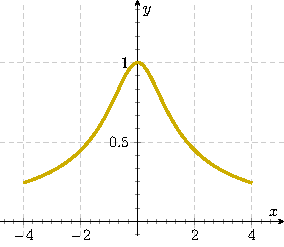
\includegraphics[width=0.5\linewidth]{mai_fig009.pdf}
   \captionof{figure}{Graf funkce $f(x):y=\dfrac{1}{1+x^2}$}
   \label{mai_fig009}
  \par}
  
  Neexistuje tedy kladné číslo, jež by bylo dolní mezí množiny funkčních hodnot, takže infimum je 
  $0$. Graf funkce $f$ je na obr. \ref{mai_fig009}.
\end{example}
      %-------------------------------------
       
      \subsubsection{Monotonní funkce}
        \begin{definition}\label{MA1:def_lim02}
          Funkci $f$ nazýváme \textbf{rostoucí (klesající)} na množině $A\subset D(f)$, jestliže 
          pro každé dva body $x_1, x_2\in A,\ x_1<x_2$, platí $f(x_1)<f(x_2)$ ($f(x_1)>f(x_2)$). 
          Funkci $f$ nazýváme \textbf{neklesající (nerostoucí)} na množině $A\subset D(f)$, 
          jestliže pro každé dvě body $x_1, x_2\in A,x_1<x_2$, platí $f(x_1)\leq f(x_2)$ 
          ($f(x_1)\geq f(x_2)$). Rostoucí a klesající funkce (na množině $A$) se nazývají 
          \textbf{ryze monotónní} (na množině $A$), neklesající a nerostoucí funkce (na množině 
          $A$) se nazývají monotónní (na množině $A$).    
        \end{definition}
            
        Z definice je zřejmé, že každá rostoucí funkce je zároveň neklesající a každá klesající 
        funkce je zároveň nerostoucí. Ryze monotónní funkce tvoří tedy podmnožinu množiny 
        monotónních funkcí. 
           
        \begin{example}
          Funkce $y=2x+1$ je \textbf{rostoucí} na intervalu $(-\infty, \infty)$. Platí totiž: $x_1<x_2\Rightarrow 2x_1<2x_2\Rightarrow2x_1+1<2x_2+1$.
        \end{example}
        \begin{example}
          Funkce y=[x] je \textbf{neklesající} na intervalu $(-\infty, \infty)$ (viz příklad **). 
        \end{example}
        \begin{example}
          Heavisideova funkce (viz příklad **) je \textbf{neklesající} na intervalu $(-\infty, \infty)$ (viz příklad **). 
        \end{example}       
        \begin{example}
          Funkce $y=|x|$ je \textbf{klesající} na intervalu $(-\infty, 0\rangle$ a rostoucí na intervalu $\langle0, \infty)$. 
        \end{example}  
            
        \begin{definition}\label{MA1:def_lim03}
          Funkci $f$ nazýváme \textbf{konstantní} na množině $A$, jestliže pro každé dva body $x_1, 
          x_2\in A$, platí $f(x_1)=f(x_2)$. V tom případě existuje reálné číslo $k$ takové, že pro 
          každé $x\in A$ je $f(x)=k$. Je-li $k=0$, mluvíme o nulové funkci na množině $A$. 
        \end{definition} 
          
        Výrok \uv{funkce $f$ je konstantní na množině $A$} zapisujeme též $f(x)=\text{konst na }A$. 
        Funkci konstantní na $\realset$ budeme stručně nazývat \textbf{konstantní funkcí} nebo 
        krátce \textbf{konstantou}. Z textu bude obvykle patrno, interpretujeme-li symbol $k$ jako 
        reálné číslo nebo jako konstantní funkci. Je zřejmé, že konstantní funkce na množině $A$ je 
        zároveň neklesající i nerostoucí na množině $A$. Toto tvrzení se dá obrátit. Lze snadno 
        dokázat i tuto větu:        
        \begin{lemma}\label{MA1:lem_lim01}
          Funkce $f$ je \textbf{rostoucí} na množině $A$, právě když je neklesající na množině $A$ a na žádné dvoubodové podmnožině $B\subset A$ není konstantní. 
        \end{lemma}
        Obdobná tvrzení platí i pro klesající funkce. 
               
      \subsubsection{Sudé a liché funkce}
        \begin{definition}\label{MA1:def_lim04}
          Funkce $f$ se nazývá \textbf{sudá} jestliže pro každé $x\in D(f)$ je též $-x\in D(f)$  a 
          platí $f(x)=f(-x)$.
          Funkce $f$ se nazývá \textbf{lichá} jestliže pro každé $x\in D(f)$ je též $-x\in D(f)$  a 
          platí $f(-x)=-f(x)$. 
        \end{definition}
        Graf sudé funkce je souměrný podle osy $y$ (osy funkčních hodnot), graf liché funkce je  
        souměrný podle počátku. 
 
       %-------------------------------------
         % !TeX spellcheck = cs_CZ
\wikitextrule
\begin{example}\label{MAI:exam024} 
  Funkce $f:\,y=x^2$ je sudá, funkce $g:\,y=x^3$ je lichá.
  
  {\centering
   \begin{tabular}{cc}
     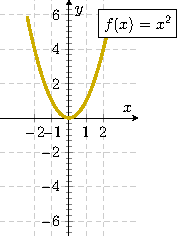
\includegraphics[width=0.5\linewidth]{mai_fig010.pdf}              &
     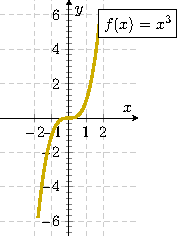
\includegraphics[width=0.5\linewidth]{mai_fig011.pdf}             \\
  \end{tabular}
  \captionsetup{type=figure}
  \captionof{figure}{Příklad sudé a liché funkce}\label{MAI:fig_002}
  \par}
\end{example}
       %-------------------------------------

        Daná funkce nemusí být ovšem ani sudá, ani lichá. Snadno se dokáže tvrzení:
        \begin{itemize}
          \item Je-li sudá funkce $f$ na množině $D(f)\cap\langle0,\infty)$ rostoucí (klesající),
                je na množině $D(f)\cap(-\infty,0\rangle$ klesající (rostoucí).
          \item Je-li lichá funkce na množině $D(f)\cap\langle0,\infty)$ rostoucí (klesající),
                je též na množině $D(f)\cap(-\infty,0\rangle$ klesající (rostoucí).                 
        \end{itemize}
      \subsubsection{Periodická funkce}

    \subsection{Operace s funkcemi. Uspořádání}
      Jak s funkcemi počítat? Definujeme základní operace s nimi — \emph{součet funkcí, součin 
      funkcí a násobení funkce reálným číslem}. Předpokládejme, že na definičním oboru 
      \(\mathcal{D}\) jsou zadány funkce \(f\) a \(g\) a reálné číslo \(\alpha\). Pak na tomtéž 
      definičním oboru lze zadat nové funkce
      \begin{align*}
        \mathcal{F} &: \mathcal{D}\ni x\,\rightarrow\,\mathcal{F}(x) = f(x)+g(x)  \in\realset   \\
        \mathcal{G} &: \mathcal{D}\ni x\,\rightarrow\,\mathcal{G}(x) = \alpha g(x)\in\realset   \\
        \mathcal{H} &: \mathcal{D}\ni x\,\rightarrow\,\mathcal{H}(x) = f(x) g(x)  \in\realset 
      \end{align*}
      Funkce \(\mathcal{F}\), \(\mathcal{G}\) a \(\mathcal{H}\) nazýváme postupně součtem funkcí 
      \(f\) a \(g\), \(\alpha\)-násobkem funkce \(f\) a součinem funkcí \(f\) a \(g\). Značíme
      \begin{equation*}
       \mathcal{F} = f + g, \qquad \mathcal{G} = \alpha f, \qquad \mathcal{H} = fg. 
      \end{equation*}
      
      Všimněme si nyní pravidel pro počítání s funkcemi zadanými na \(\mathcal{D}\) a zjistíme, 
      že se velmi podobají pravidlům pro počítání s reálnými čísly. Není divu, vždyť operace s 
      funkcemi jsou definovány prostřednictvím funkčních hodnot, a těmi jsou reálná čísla. Některé 
      důležité odlišnosti však přece jen najdeme. Napřed ale pravidla:
      
      \begin{itemize}\addtolength{\itemsep}{-0.5\baselineskip}
        \item komutativní zákon pro součet funkcí
          \begin{equation}\label{mai:eq012}
            f(x) + g(x) = g(x) + f(x)
          \end{equation}
        \item asociativní zákon pro součet funkcí  
          \begin{equation}\label{mai:eq013}
            (f(x) + g(x)) + h(x) = f(x) + (g(x) + h(x)
          \end{equation}
        \item existence univerzálního neutrálního  prvku \(O\) (nulová funkce \(O:\mathcal{D}\ni x 
          \rightarrow O(x)=0\))
          \begin{equation}\label{mai:eq014}
            f(x) + O = O + f(x) = f(x)
          \end{equation}
        \item existence právě jednoho opačného prvku k funkci \(f\), přičemž \((-f)(x) = -f(x)\)
          \begin{equation}\label{mai:eq015}
            f(x)+(-f(x))=(-f(x))+f(x)=O
          \end{equation}
        \item asociativní zákon pro násobení číslem 
         \begin{equation}\label{mai:eq016}
            (\alpha_1\alpha_2)f(x) = \alpha_1(\alpha_2f(x))
         \end{equation}
        \item  1. distributivní zákon pro násobení číslem
          \begin{equation}\label{mai:eq017}
            \alpha(f(x)+g(x) =\alpha f(x) + \alpha g(x)
          \end{equation}\label{mai:eq018}
        \item 2. distributivní zákon pro násobení číslem 
          \begin{equation}\label{mai:eq019}
            (\alpha_1+\alpha_2)f(x) =\alpha_1f(x)+\alpha_2f(x)
          \end{equation}
        \item násobení číslem \((—1)\) dává opačný prvek
          \begin{equation}\label{mai:eq020}
            (-1)f(x)=(-f(x))
          \end{equation}
        \item komutativní zákon pro součin funkcí
          \begin{equation}\label{mai:eq021}
            f(x)g(x)=g(x)f(x)
          \end{equation}
        \item asociativní zákon pro součin funkcí 
          \begin{equation}\label{mai:eq022}
            f(x)(g(x)h(x))=(f(x)g(x))h(x)
          \end{equation}
        \item distributivní zákon zprava pro součin funkcí
          \begin{equation}\label{mai:eq023}
            (f_1(x) + f_2(x))g(x) =f_1(x)g(x) + f_2(x)g(x)
          \end{equation}
        \item distributivní zákon zleva pro součin funkcí
          \begin{equation}\label{mai:eq024}
            f(x)(g_1(x) + g_2(x))=f(x)g_1(x)+f(x)g_2(x)
          \end{equation}
        \item násobení jednotkovou funkcí \(I: \mathcal{D}\ni x \rightarrow I(x) = 1\)  
          \begin{equation}\label{mai:eq025}
           f(x)I=If(x)
          \end{equation}
        \item existence právě jedné \emph{převrácené} funkce k funkci \(f\) pro \(f(x)\neq0\quad 
              (f)^{-1}: \bar{D}\ni x\rightarrow (f)^{-1}(x)=[f(x)]^{-1}\) kde \(\bar{\mathcal{D}} 
              = \mathcal{D} - \left\{x\in \mathcal{D}\,|\,f(x)=0\right\}\)
          \begin{equation}
            f(x)(f(x))^{-1}=(f(x))^{-1}f(x) = I
          \end{equation}
      \end{itemize}
      Všimněme si, že funkce \((f)^{-1}\) existuje obecně na užším definičním oboru 
      \(\bar{\mathcal{D}}\), než na kterém je definována funkce \(f\). Je totiž třeba vyloučit 
      všechny hodnoty \(x\), pro které \(f(x) = 0\) (zákaz dělení nulou). K funkci \(O\) tedy 
      převrácená funkce neexistuje vůbec!
      
      Existence opačné a převrácené funkce k \(f\) umožňuje definovat \emph{rozdíl} a \emph{podíl} 
      funkcí \(f-g=f+(-g)\) a \(\dfrac{f}{g}=f(g)^{-1}\), tj.
      \begin{align*}
        f-g         &: \mathcal{D}\ni x\,\rightarrow\, (f-g)(x)=f(x)+(-g)(x)= f(x)-g(x), \\
        \frac{f}{g} &: \bar{D}\ni x\,\rightarrow\, 
                       \left(\frac{f}{g}\right)(x) = f(g)^{-1}(x) = \frac{f(x)}{g(x)}, 
      \end{align*}
      kde \(\bar{D}=D-\left\{x\in D\,|\,g(x)=0 \right\}\) 
      
      \begin{note}
        Pamatujme si označení převrácené funkce jako \((f)^{-1}\), v němž je zápis symbolu \(f\) do 
        závorky podstatný. Jde o něco jiného než znamená symbol \(f^{-1}\) bez závorky, který 
        rezervujeme pro inverzní funkci v dalším výkladu.
      \end{note}
      \begin{note}
        Porovnáme-li nyní vlastnosti operací s funkcemi a pravidla pro počítání s reálným čísly, 
        komplexními čísly, maticemi a vektory, můžeme konstatovat, že množina funkcí s operací 
        sčítání funkcí a násobení funkce číslem je \textbf{vektorovým prostorem}. To je vlastnost, 
        která je s případem čísel, matic a vektorů společná. Vektorový prostor funkcí se však od 
        zmiňovaných vektorových prostorů výrazně liší svou dimenzí (rozměrem). Intuitivně dobře 
        chápeme, co znamená jednorozměrný, dvojrozměrný a trojrozměrný prostor (například 
        \(\realset^1\), \(\realset^2\), \(\realset^3\)). V odstav 1.4 jsme dokonce pracovali v 
        n-rozměrném vektorovém prostoru. Dimenze vektorového prostoru může být i nekonečná — třeba 
        zrovna u funkcí. Obecně jde o pojem poměrně obtížný a budeme se jím důkladně zabývat až v 
        kapitolách věnovaných algebře \cite[s.~58]{Musilova2009MA1}.
      \end{note}
      
      Operace s funkcemi jsme definovali a prodiskutovali pro případ, kdy definiční obory funkcí, 
      vstupujících do operace byly stejné. Co když tomu tak nebude? Znamená to, že pak nemůžeme 
      funkce sčítat, násobit, apod.? Předpokládejme, že definičním oborem funkce \(f\) je množina 
      \(\mathcal{D}_f\) definičním oborem funkce \(g\) množina \(D_g\). Pokud jsou tyto obory 
      disjunktní, tj. \(\mathcal{D}_f \cap \mathcal{D}_g = 0\), můžeme utvořit pouze 
      \(\alpha\)-násobek funkce \(f\) či \(g\). Sčítat ani násobit funkce \(f\) a \(g\) nemůžeme 
      neboť hodnota \(f(x) + g(x)\) ani \(f(x)g(x)\) neexistuje pro žádné \(x\). Pokud je průnik 
      \(D=d_f\cap D_g\) oborů \(\mathcal{D}_f\) a \(\mathcal{D}_g\) neprázdný, stává se definičním 
      oborem funkcí \(f+g\) a \(fg\). Platí stejná pravidla jako v předchozí tabulce, pouze s 
      omezením na obor \(\mathcal{D}_f\).
    
    \subsection{Skládání a inverze funkcí}
      \emph{Skládání} neboli kompozici funkcí si lze snadno představit opět pomocí „černých 
      skříněk“ (obr. \ref{mai:fig012}): Do první skřínky představující předpis \(g\), \emph{vnitřní 
      složku} složené funkce, vstupuje
      \begin{figure}[ht!] %\ref{mai:fig012}
        \centering
%        % !TeX spellcheck = cs_CZ
% exam017.tex

\documentclass[11pt]{standalone}
\usepackage{xltxtra}
\usepackage[usenames,x11names]{xcolor}
\usepackage{tikz}
\usepackage{pgfplots}
  \pgfplotsset{compat=newest}
\usepackage{amsmath}
\usepackage{amsfonts}          % \mathbb{R}
  \newcommand{\realset}{\mathbb{R}}

\begin{document}
  \begin{tikzpicture}[fill=black!20]
  %  \draw[help lines] (-1,-2) grid (6,3);
    \path (0,0) node(a) [ ] {\(\mathcal{D}_g\)}
    (2,0) node(b) [rectangle,rotate=0,draw,fill] 
      {\(\begin{array}{c} \text{funkce} \\ g  \end{array}\)}
    (4.5,0) node(c) [rectangle,rotate=0,draw,fill] 
      {\(\begin{array}{c} \text{funkce} \\ f  \end{array}\)}
    (7,0) node(d) [ ] {\(\realset\)};
    \draw[thick,->] (a.east) -- (b);
    \draw[thick,->] (b.east) -- (c);
    \draw[thick,->] (c.east) -- (d);
    \path [ ] (a.east) -- (b.west)   node [above,midway] {\(x\)};
    \path [ ] (b.east) -- (c.west)   node [above,midway] {\(g(x)\)};
    \path [ ] (c.east) -- (d.west)   node [above,midway] {\(f[g(x)]\)};
  \end{tikzpicture}
\end{document}
        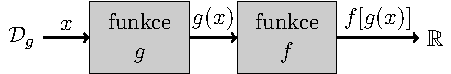
\includegraphics[width=0.45\linewidth]{mai_fig012.pdf}
        \caption{Skládání funkcí \cite[s.~59]{Musilova2009MA1}}
        \label{mai:fig012}
      \end{figure}
      hodnota \(x\) z definičního oboru \(\mathcal{D}_g\) funkce \(g\). Výstupem je číslo \(u = 
      g(x)\), funkční hodnota vnitřní složky v bodě \(x\). Toto číslo smí vstoupit do skříňky 
      představující předpis \(f\), \emph{vnější složku} složené funkce, právě tehdy, je-li prvkem 
      jejího definičního oboru \(\mathcal{D}_f\). V takovém případě najdeme na výstupu ze skříňky 
      \(f\) hodnotu \(y = f(u) = f[g(x)]\). (Jestliže \(g(x)\notin\mathcal{D}_f\), není výstup ze 
      skříňky \(f\) definován.) Vzniká nový předpis \(F\), kterým se některým bodům definičního 
      oboru \(\mathcal{D}_g\), ne všem, ale pouze těm, pro něž \(g(x)\in\mathcal{D}_f\), 
      přiřazují hodnoty \(f[g(x)]\). Definujme nyní složenou funkci přesněji: Předpokládejme, že 
      jsou zadány funkce
      \begin{align*}
        g  &: \mathcal{D}_g\ni x\,\rightarrow\, g(x) = u\in\realset, \\
        f  &: \mathcal{D}_f\ni u\,\rightarrow\, f(u) = y\in\realset. \\
        \shortintertext{označme}
        \mathcal{D} &= \{x|x\in\mathcal{D}_g \text{ a současně } g(x)\in\mathcal{D}_f\}.
      \end{align*}
      Pokud \(\mathcal{D} = \emptyset\), lze definovat funkci
      \begin{equation*}
        F: \mathcal{D}\ni x\rightarrow y = F(x) = f[g(x)]\in\realset, 
           \text{ značíme } F = f \circ g.
      \end{equation*}
      \(F\) se nazývá \emph{složením} neboli \emph{kompozicí} funkcí \(g\) a \(f\). Zápis \(f\circ 
      g\) čteme často také jako \emph{„f po g“}. Skládat lze i větší počet funkcí.

       %-------------------------------------
         % !TeX spellcheck = cs_CZ
\begin{mdframed}[style=mdexam]
  \begin{example}\label{MAI:exam025}
    Uvažme funkci z příkladu \ref{vol02:fyz:fey_exam017}. 
    
    {\centering
    \captionsetup{type=figure}
  %   % !TeX spellcheck = cs_CZ
\documentclass[11pt]{standalone}
\usepackage{xltxtra}
\usepackage[usenames,x11names]{xcolor}
\usepackage{tikz}
\usepackage{pgfplots}
  \pgfplotsset{compat=newest}
\usepackage{amsmath}

\begin{document}
  \begin{tikzpicture}[thick,scale=0.7, every node/.style={transform shape}]
    \begin{axis}[
      xmin = -5, xmax = 5, ymin = -10, ymax = 1.5,
   %   domain = -0.999999:0.999999,
      restrict y to domain=-30:1.5,
      unit vector ratio=1 1 1,  % axis equal
      grid = both,   % both, major
      grid style={line width=.1pt, draw=gray!20},
      major grid style={dashed, line width=.2pt, draw=gray!40},
      minor tick num=4,
      clip = true,
      clip mode=individual,
      axis x line = middle,
      axis y line = middle,
      xlabel={$x$},
    %  xlabel style={at=(current axis.right of origin), anchor=west},
      ylabel={$u,w,y$},
    %  ylabel style={at=(current axis.above origin), anchor=south},
      enlarge y limits={rel=0.13},
      enlarge x limits={rel=0.07},
    ]
    
      \addplot[color=Gold3, samples=1000, smooth, ultra thick, unbounded coords=jump, no markers, 
               domain = -0.999999:0.999999] 
        gnuplot{log10(sqrt(1-x^2))/log10(2)};  
        
     \addplot[color=green, samples=200, smooth, ultra thick, unbounded coords=jump, no markers, 
     domain = -3.3:3.3] 
        gnuplot{1-x^2};
        
     \addplot[color=blue, samples=200, smooth, ultra thick, unbounded coords=jump, no markers, 
     domain = -1:1] 
        gnuplot{sqrt(1-x^2)};  
    \end{axis}
  \end{tikzpicture}
\end{document}
    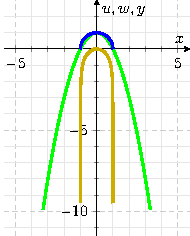
\includegraphics[width=0.6\linewidth]{mai_fig013.pdf}
    \captionof{figure}{K příkladu \ref{MAI:exam025} \(y=\log_2{(\sqrt{1-x^2})}\) 
    \cite[s.~57]{Musilova2009MA1}
    \label{mai:fig013}}
    \par}
    
    Ukážeme, jak tato funkce vzniká postupně složením tří funkcí a jak při tom dochází k postupnému 
    omezování definičního oboru. Písmeny \(\mathcal{D}\) a \(H\) s příslušným indexem budeme značit 
    definiční obory a obory hodnot jednotlivých funkcí.
    \begin{gather*}
      \begin{align*}
        g&:  \realset =\mathcal{D}_g\ni x\rightarrow u=g(x) = 1- x^2  \in\mathcal{H}_g=(-\infty,1], \\
        h&: [0,\infty)=\mathcal{D}_h\ni u\rightarrow w=h(u) = \sqrt{u}\in\mathcal{H}_h=[0,\infty),  \\
       \shortintertext{\(\mathcal{D}_h\cap\mathcal{H}_g = [0,1]\Rightarrow\mathcal{D}_{h\circ g}=[-1,1], 
                       \mathcal{H}_{h\circ g} = [0,1],\)}                                    \\
       f&:(0,\infty)=\mathcal{D}_f\ni w \rightarrow y=f(w)=\log_2w\in\mathcal{H}_f=\realset  \\
       \shortintertext{\(\mathcal{H}_{h\circ g}\cap\mathcal{D}_f = (0,1] 
                       \Rightarrow\mathcal{D}_F=(-1,1),\mathcal{H}_F=(-\infty,0].\)} 
      \end{align*}
    \end{gather*}
    Je tedy
    \begin{gather*}
      \begin{align*}
        F:\mathcal{D}_F\ni x\rightarrow 
        y&=F(x)=(f\circ(h\circ g))(x) = f{h[g(x)]}          \\
        &= \log_2\sqrt{1-x^2}\in(-\infty,0].
      \end{align*}
    \end{gather*}
    Názorněji než tento zápis ukazuje situaci obrázek \ref{mai:fig013}.
  \end{example}
\end{mdframed}
       %-------------------------------------
      
      Může vzniknout otázka, jak rozpoznáme vnitřní a vnější složku složené funkce. Rozlišit 
      vnitřní a vnější složku třeba u funkcí \(\cos(x^2)\) a \((cos x)^2\) není problém. Hned také 
      vidíme, že obecně \(f\circ g\neq g\circ f\), i když by definiční obory funkcí na pravé i levé 
      straně měly neprázdný průnik. Jsou však i případy na první pohled méně zřetelné, jak ukazuje 
      následující příklad.
      
      %-------------------------------------
        % !TeX spellcheck = cs_CZ
\begin{mdframed}[style=mdexam]
  \begin{example}\label{mai:exam026}
    (Určení vnitřní a vnější složky) Uveďme příklad dvou funkcí \(F(x)=\sqrt{x^2}\) a \(G(x) =
    (\sqrt{x})^2\). Liší se tyto funkce, nebo jde o tutéž funkci, jen jinak zapsanou? Vidíme, že
    platí

    \begin{align*}
      \mathcal{D}_F &=\realset, F(x)=\abs{x}\forall x\in\mathcal{D}_F, \mathcal{H}_F = [0, infty),\\
      \mathcal{D}_G &=[0, \infty), G(x)=x\forall    x\in\mathcal{D}_G, \mathcal{H}_G = [0, infty).
    \end{align*}
    Funkce \(F\) a \(G\) mají různé definiční obory, ale na jejich průniku dávají stejné funkční
    hodnoty. Ani zde však obecně nelze pořadí skládání funkcí zaměňovat.
  \end{example}
\end{mdframed}
      %-------------------------------------
       
      Funkce \(F\) a \(G\) mají různé definiční obory, ale na jejich průniku dávají stejné funkční 
      hodnoty. Ani zde však obecně nelze pořadí skládání funkcí zaměňovat.
      
      Nyní se pusťme do vybudování pojmu inverzní funkce k funkci \(f\). Představme si, že funkční
      hodnota \(y = f(x)\) zadané funkce
      \begin{equation*}
        f: \mathcal{D}_f\ni x \rightarrow f(x)\in\mathcal{H}_f
      \end{equation*}
      představuje „zakódovanou“ informaci o hodnotě \(x\). Položme si otázku, zda a za jakých 
      podmínek dokážeme sestavit „černou skříňku“, na jejímž výstupu by se při vstupu obrazu \(y = 
      f(x)\) objevila hodnota \(x\). Omezení takové možnosti je názorně vidět na obrázku 
      \ref{mai:fig014}. V případě funkce \(f(x)\) lze ke všem obrazům \(y \in \mathcal{H}_f\) najít 
      vzory, v případě funkce \(g(x)\) to možné není, neboť jeden a týž obraz lze získat z několika 
      vzorů. Pro který bychom se tedy měli rozhodnout?
      
      \begin{figure}[ht!] %\ref{mai:fig014}
        \centering
%        % !TeX spellcheck = cs_CZ
% Skládání funkcí \cite[s.~61]{Musilova2009MA1}

\documentclass[11pt]{standalone}
\usepackage{xltxtra}
\usepackage[usenames,x11names]{xcolor}
\usepackage{tikz}
\usepackage{pgfplots}
  \pgfplotsset{compat=newest}
\usepackage{amsmath}
\usepackage{amsfonts}       % \mathbb{R}
  \newcommand{\realset}{\mathbb{R}}

\begin{document}
  \begin{tikzpicture}[fill=black!20]
  %  \draw[help lines] (-1,-2) grid (6,3);
    \path (0,0) node(a) [ ] {\(\mathcal{D}_f\)}
    (2,0) node(b) [rectangle,rotate=0,draw,fill] 
      {\(\begin{array}{c} \text{funkce} \\ f  \end{array}\)}
    (4.5,0) node(c) [rectangle,rotate=0,draw,fill] 
      {\(\begin{array}{c} \text{funkce} \\ f^{-1}  \end{array}\)}
    (7,0) node(d) [ ] {\(\realset\)};
    \draw[thick,->] (a.east) -- (b);
    \draw[thick,->] (b.east) -- (c);
    \draw[thick,->] (c.east) -- (d);
    \path [ ] (a.east) -- (b.west)   node [above,midway] {\(x\)};
    \path [ ] (b.east) -- (c.west)   node [above,midway] {\(f(x)\)};
    \path [ ] (c.east) -- (d.west)   node [above,midway] {\(x\)};
  \end{tikzpicture}
\end{document}
        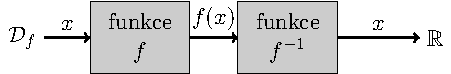
\includegraphics[width=0.45\linewidth]{mai_fig014.pdf}
        \caption{Skládání funkcí \cite[s.~61]{Musilova2009MA1}}
        \label{mai:fig014}
      \end{figure}
       Aby bylo možné vzor zpětně identifikovat na základě znalosti obrazu, je třeba, aby funkce 
       \(f\) byla \emph{prostá}, tj. aby předpis \(f\) přiřazoval každým dvěma různým vzorům \(X_1 
       \neq x_2\) dva různé obrazy \(f(x_1) \neq f(x_2)\). Často lze tohoto požadavku docílit tím, 
       že se místo funkce \(f\) s definičním oborem \(\mathcal{D}_f\) spokojíme s funkcí, která 
       vznikne omezením \emph{(restrikcí)} té původní na „menší“ definiční obor, zato však již bude 
       prostá. U funkce \(g\) na obrázku \ref{mai:fig016} by tak stačilo omezit definiční obor 
       například na množinu \(\mathcal{D}_g\). Než inverzní funkci definujeme, ukažme si způsob 
       jejího nalezení na známém příkladu.

       \begin{figure}[ht!]
         \centering  
         \begin{tabular}{cc}
           \subfloat[ ]{\label{mai:fig016a}
             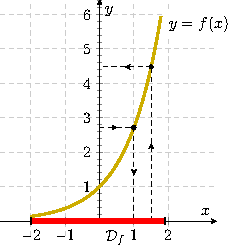
\includegraphics[width=0.45\linewidth]{mai_fig016a.pdf}}              &
           \subfloat[ ]{\label{mai:fig016b}
             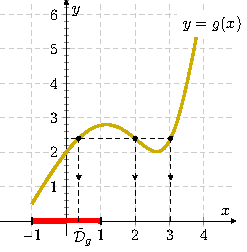
\includegraphics[width=0.45\linewidth]{mai_fig016b.pdf}}              \\
         \end{tabular}
         \caption{K pojmu inverzní funkce}
         \label{mai:fig016}
       \end{figure}
      
      %-------------------------------------
        % !TeX spellcheck = cs_CZ
\begin{mdframed}[style=mdexam]
  \begin{example}\label{MAI:exam027}
    (Nalezení inverzní funkce): Funkci 
    \begin{equation*}
      y = \log_2(\sqrt{1-x^2})
    \end{equation*}
    Jsme již z různých hledisek rozebrali v příkladech \ref{vol02:fyz:fey_exam017} a
    \ref{MAI:exam025}. Hodí se i nyní.

    {\centering
    \captionsetup{type=figure}
  %  % !TeX spellcheck = cs_CZ
% K příkladu \ref{mai:exam027} \(y=\log_2{(\sqrt{1-x^2})}

\documentclass[11pt]{standalone}
\usepackage{xltxtra}
\usepackage[usenames,x11names]{xcolor}
\usepackage{tikz}
\usepackage{pgfplots}
  \pgfplotsset{compat=newest}
\usepackage{amsmath}

\begin{document}
  \begin{tikzpicture}[thick,scale=0.7, every node/.style={transform shape}]
    \begin{axis}[
      xmin = -5, xmax = 5, ymin = -5, ymax = 1.5,
   %   domain = -0.999999:0.999999,
      restrict y to domain=-30:1.5,
      unit vector ratio=1 1 1,  % axis equal
      grid = both,   % both, major
      grid style={line width=.1pt, draw=gray!20},
      major grid style={dashed, line width=.2pt, draw=gray!40},
      minor tick num=4,
      clip = true,
      clip mode=individual,
      axis x line = middle,
      axis y line = middle,
      xlabel={\(x\)},
    %  xlabel style={at=(current axis.right of origin), anchor=west},
      ylabel={\(y\)},
    %  ylabel style={at=(current axis.above origin), anchor=south},
      enlarge y limits={rel=0.13},
      enlarge x limits={rel=0.07},
    ]
    
      \addplot[color=Gold3, samples=1000, smooth, ultra thick, unbounded coords=jump, no markers, 
               domain = 0:0.9995] 
        gnuplot{log10(sqrt(1-x^2))/log10(2)};  
        
      \addplot[color=blue, samples=200, smooth, ultra thick, unbounded coords=jump, no markers, 
               domain = -5:0] 
        gnuplot{sqrt(1-2^(2*x))};  
    \end{axis}
  \end{tikzpicture}
\end{document}
    \luafigure[0.9]{mai_fig015.pdf}
    \captionof{figure}{K příkladu \ref{MAI:exam027} \(y=\log_2{(\sqrt{1-x^2})}\) 
    \cite[s.~62]{Musilova2009MA1}
    \label{mai:fig015}}
    \par}
    
    Na obrázku \ref{mai:fig013} máme dokonce její graf, a tak vidíme, že \textbf{není} na svém 
    definičním oboru \((-1, 1)\) \textbf{prostá}. Omezme proto její definiční obor na interval 
    \(\mathcal{D} = [0, 1)\), na němž již prostá je (část grafu vpravo od osy \(y\)). Pro danou 
    hodnotu obrazu \(y \in (-\infty,0]\) můžeme již jednoznačně určit hodnotu \(x\) jednoduchou 
    úpravou:
    \begin{align*}
      y = \log_2(\sqrt{1-x^2}) &\Rightarrow \sqrt{1-x^2} = 2^y   \\
                               &\Rightarrow x^2 = 1 - 2^{2y}     \\
                               &\Rightarrow x = \sqrt{1 - 2^{2y}}
    \end{align*}
    Formální záměnou \(x \leftrightarrow y\) dostáváme inverzní funkci k funkci \(f\),
    \begin{equation*}
      y =f^{-1}(x) = \sqrt{1 - 2^{2x}}.
    \end{equation*}
    Grafy obou funkcí jsou na obrázku \ref{mai:fig015}.
  \end{example}
\end{mdframed}
      %-------------------------------------
      
      Ze způsobu konstrukce funkce \(f^{-1}\) v předchozím příkladu je vidět, že 
      \(\mathcal{D}_{f^{-1}} = \mathcal{H}_f\), \(\mathcal{H}_{f^{-1}} = \mathcal{D}_f\) a graf 
      inverzní funkce je obrazem grafu prosté funkce \(f\) při osové symetrii v rovině 
      souřadnicových os vzhledem k ose prvního a třetího kvadrantu. Nyní již definujeme inverzní 
      funkci obecně. Předpokládejme, že funkce \(f : \mathcal{D}_f\ni x \rightarrow y = f(x)\ni 
      \mathcal{H}_f\) je prostá na svém definičním oboru. Pak existuje funkce \(f^{-1}\) definovaná 
      jako
      \begin{equation}\label{mai:eq029}
        f^{-1} :\mathcal{H}_f\ni x\rightarrow y = f^{-1}(x)\in\mathcal{D}_f\Leftrightarrow x = f(y).
      \end{equation}
      Funkci \(f^{-1}\) nazýváme \textbf{inverzní funkcí k funkci} \(f\). Ještě shrneme pravidla 
      pro skládání funkcí a pro inverzní funkce:

      \begin{itemize}\addtolength{\itemsep}{-0.5\baselineskip}
        \item asociativní zákon pro skládání funkcí
          \begin{equation}\label{mai:eq030}
            f(x)\circ(h(x)\circ g(x)) = f(x)\circ h(x) \circ g(x)
          \end{equation}
        \item distributivní zákon zleva 
          \begin{equation}\label{mai:eq031}
            f(x) \circ (h(x) + g(x)) = f(x) \circ h(x) + f(x) \circ g(x)
          \end{equation}
        \item existence univerzálního neutrálního  prvku \(O\) (nulová funkce \(O:\mathcal{D}\ni x 
          \rightarrow O(x)=0\))
          \begin{equation}\label{mai:eq032}
            f(x) + O = O + f(x) = f(x)
          \end{equation}
        \item existence právě jednoho opačného prvku k funkci \(f\), přičemž \((-f)(x) = -f(x)\)
          \begin{equation}\label{mai:eq033}
            f(x)+(-f(x))=(-f(x))+f(x)=O
          \end{equation}
        \item komutativní zákon pro součet funkcí
          \begin{equation}\label{mai:eq034}
            f(x) + g(x) = g(x) + f(x)
          \end{equation}
        \item asociativní zákon pro součet funkcí  
          \begin{equation}\label{mai:eq035}
            (f(x) + g(x)+h(x) = f(x) + (g(x) + h(x)
          \end{equation}
        \item existence univerzálního neutrálního  prvku \(O\) (nulová funkce \(O:\mathcal{D}\ni x 
          \rightarrow O(x)=0\))
          \begin{equation}\label{mai:eq036}
            f(x) + O = O + f(x) = f(x)
          \end{equation}        
      \end{itemize}   
      Předchozí vztahy platí na patřičně zúžených definičních oborech funkcí, které do nich 
      vstupují.
      
  %-------------------------------------------------------------------------------------------------
  \section{Elementární funkce}
      Základními elementárními funkcemi nazýváme \cite[s.~10]{PolakMA1}:
%      \begin{displaymath}
%        \xymatrix{
%        \mbox{mocninné} & *+[F]{\mbox{Elementární 
%        funkce}}\ar@{->}[l]\ar@{->}[dl]\ar@{->}[d]\ar@{->}[dr]\ar@{->}[r]&\mbox{exponenciální} \\
%        \mbox{goniometrické}       &   \mbox{logaritmické}      & \mbox{cyklometrické}
%        }
%      \end{displaymath}
    %------------- Goniometrické funkce ------------------------------------------------------------
    \subsection{Goniometrické funkce}  
    \begin{itemize}
      \item \textbf{Základní vzorce pro goniometrické funkce}
        \begin{align}
          \sin^2\alpha     &+ \cos^2\alpha = 1      &\forall\alpha\in\realset \label{MA1:eq_sincos} \\ 
          \abs{\sin\alpha} &= \sqrt{1-\cos^2\alpha} &\forall\alpha\in\realset \label{MA1:eq_sinabs} \\ 
          \abs{\cos\alpha} &= \sqrt{1-\sin^2\alpha} &\forall\alpha\in\realset \label{MA1:eq_cosabs}
        \end{align}  
      \item \textbf{Součtové vzorce}
        \begin{align}
        % \nonumber to remove numbering (before each equation)
          \sin(\alpha + \beta) 
            &= \sin\alpha\cdot\cos\beta 
             - \sin\beta\cdot\cos\alpha           \label{MA1:eq_sinxpy}  \\ 
          \sin(\alpha - \beta) 
            &= \sin\alpha\cdot\cos\beta 
             + \sin\beta\cdot\cos\alpha           \label{MA1:eq_sinxmy}  \\ 
          \cos(\alpha + \beta) 
            &= \cos\alpha\cdot\cos\beta 
             - \sin\alpha\cdot\sin\beta           \label{MA1:eq_cosxpy}  \\ 
          \cos(\alpha - \beta) 
            &= \cos\alpha\cdot\cos\beta 
             + \sin\alpha\cdot\sin\beta           \label{MA1:eq_cosxmy}  \\ 
          \tan(\alpha\pm\beta) 
            &= \frac{\tan\alpha\pm\tan\beta}{1\mp\tan\alpha\cdot\tan\beta} \label{MA1:eq_tanxpmy}\\ 
          \cot(\alpha\pm\beta) 
            &= \frac{1\mp\cot\alpha\cdot\cot\beta}{\cot\alpha\pm \cot\beta} \label{MA1:eq_cotxpmy}
        \end{align}
        Součtové vzorce lze odvodit několika způsoby; jednoduchý způsob důkazu
        lze provést pomocí skalárního součinu vektorů.
      \item \textbf{Vzorce pro dvojnásobný úhel $2\alpha$}
        \newline Pro každé $\alpha\in R$ platí:
        \begin{align}
          \sin(2\alpha)   &= 2\sin\alpha\cos\alpha                \label{MA1:eq_sin2x} \\ 
          \cos(2\alpha)   &= \cos^2\alpha - \sin^2\alpha          \label{MA1:eq_cos2x} \\ 
          \tan(2\alpha)   &= \frac{2\tan\alpha}{1-\tan^2\alpha}   \label{MA1:eq_tan2x} \\ 
          \cot(2\alpha)   &= \frac{\cot^2\alpha - 1}{2\cot\alpha} \label{MA1:eq_cot2x}
        \end{align}
      \item \textbf{Vzorce pro poloviční úhel $\displaystyle\frac{\alpha}{2}$}
        \begin{align}
          \left\lvert\sin\frac{\alpha}{2}\right\rvert   
            &= \sqrt{\frac{1-\cos\alpha}{2}}                      \label{MA1:eq_sinx2} \\ 
          \left\lvert\cos\frac{\alpha}{2}\right\rvert   
            &= \sqrt{\frac{1+\cos\alpha}{2}}                      \label{MA1:eq_cosx2} \\ 
          \left\lvert\tan\frac{\alpha}{2}\right\rvert   
            &= \sqrt{\frac{1-\cos\alpha}{1+\cos\alpha}}           \label{MA1:eq_tanx2} \\ 
          \left\lvert\cot\frac{\alpha}{2}\right\rvert   
            &= \sqrt{\frac{1+\cos\alpha}{1-\cos\alpha}}           \label{MA1:eq_cotx2}
        \end{align}
    \end{itemize}
    Vzorce \ref{MA1:eq_sinx2} a \ref{MA1:eq_cosx2} odvodíme pomocí vzorců \ref{MA1:eq_cos2x} a \ref{MA1:eq_sincos}:
    \begin{align*}
      \cos\alpha &= 
      \cos2\frac{\alpha}{2}=\cos^2\frac{\alpha}{2}-\sin^2\frac{\alpha}{2}=1-2\sin^2\frac{\alpha}{2} \\
      \sin^2\frac{\alpha}{2} &= \frac{1-\cos\alpha}{2}   \\
      \cos^2\frac{\alpha}{2} &= 1 - \sin^2\frac{\alpha}{2} = \frac{1+\cos\alpha}{2} 
    \end{align*}
    a dále užijeme vztahu $\sqrt{a^2}=\abs{a}$ (platí pro každé $a\in\realset$). Užitím součtových vzorců a toho že, 
	$\sin\frac{\pi}{2} = 1$, $\cos\frac{\pi}{2} = 0$, $\sin\pi = 0$ a $\cos\pi = -1$ lze snadno odvodit, 
	že pro každé $\alpha\in R$ platí
    \begin{align*}
      \sin\left(\frac{\pi}{2}+\alpha\right) &=  \cos\alpha  &   \cos\left(\frac{\pi}{2}+\alpha\right) &= -\sin\alpha \\
      \sin\left(\frac{\pi}{2}-\alpha\right) &=  \cos\alpha  &   \cos\left(\frac{\pi}{2}-\alpha\right) &=  \sin\alpha \\
      \sin\left(\pi+\alpha\right)           &= -\sin\alpha  &   \cos\left(\pi+\alpha\right)           &= -\cos\alpha \\
      \sin\left(\pi-\alpha\right)           &=  \sin\alpha  &   \cos\left(\pi-\alpha\right)           &= -\cos\alpha \\
    \end{align*}
    \newline Důkaz provedeme pro první z těchto často užitečných vzorců (u ostatních je odvození obdobné):
    $$\sin\left(\frac{\pi}{2}+\alpha\right) = \sin\frac{\pi}{2}\cos\alpha + \cos\frac{\pi}{2}\sin\alpha = 1\cdot\cos\alpha + 0\cdot\sin\alpha.$$
 
    %-----------------------------------------------------------------------------------------------
    \subsection{Zobrazení v jiných strukturách}
    %-----------------------------------------------------------------------------------------------
    \subsection{Cvičení}
  %================ Podkapitola: Limita funkce =====================================================
  \section{Limity všeho druhu}  
    „Limes“ znamená latinsky příční cesta, mez, v přeneseném významu pak hranice, pomezí, atd. V 
    matematice představuje limita hodnotu, ke které se „neomezeně blíží hodnota funkce, jestliže se 
    hodnota proměnné neomezeně blíží zadanému číslu“. Poslední formulace musí být v uvozovkách, 
    protože je i přes svou dobrou názornost velice nepřesná. A takové nepřesnosti nejsou v 
    matematice dovoleny. K čemu vůbec úvaha o limitě je? Stačí přece do funkčního předpisu hodnotu 
    proměnné dosadit a získat funkční hodnotu. Tak jednoduché to ale není. Funkční hodnota pro 
    danou hodnotu proměnné \(x\) vůbec nemusí být definována, zato může být definována pro hodnoty 
    velmi blízké. Nebo definována je, ale pro hodnoty proměnné, které jsou k \(x\) velmi blízké, 
    jsou funkční hodnoty od \(f(x)\) velmi vzdálené. Potřebnost pojmu limita ukážeme na 
    geometrickém a fyzikálním příkladu.
    
    V matematické analýze hraje např. důležitou úlohu podíl \cite[s.~117]{Brabec1989}
    \begin{equation*}
      \dfrac{\varphi(x) - \varphi(a)}{x - a}
    \end{equation*}
    kde \(\varphi\) je daná funkce, \(a\) pevný bod. Tento podíl tzv. \emph{přírůstku funkce} 
    \(\varphi(x) — \varphi(a)\) k přírůstku argumentu \(x — a\) může značit např. \emph{průměrnou 
    rychlost pohybu bodu po přímce}, jehož zákon dráhy je dán vztahem \(y = \varphi(x)\), kde \(y\) 
    je dráha, kterou bod urazí za čas \(x\). Zajímá nás, jak se mění hodnota tohoto podílu — jinak 
    řečeno, jak se mění hodnota funkce \(f\) dané vztahem
    \begin{equation}\label{mai:eq037}
      f(x) = \dfrac{\varphi(x) - \varphi(a)}{x - a}
    \end{equation}
    když hodnoty argumentu \(x\) se blíží k číslu \(a\), což často značíme \(x\rightarrow a\). V 
    uvedeném fyzikálním významu daného podílu se ptáme, jak se mění průměrná rychlost pohybu, když 
    se časový úsek zkracuje. Je zřejmé, že musí být stále \(x \neq a\) a že jmenovatel se blíží k 
    nule; obvykle se blíží k nule i čitatel. Jakých hodnot však nabývá přitom podíl, tj. jaké jsou 
    hodnoty funkce \(f(x)\)? Než vyslovíme přesnou definici limity, uvedeme ještě pár jednoduchých 
    příkladů.

    %-------------------------------------
      % !TeX spellcheck = cs_CZ
\wikitextrule
\begin{example}\label{MAI:exam028}
  Nechť \(\varphi(x) = x^2\), \(a = 1\). Potom \(f(x) = (x^2 — 1 )/(x — 1)\). Pro \(x \neq 1\) je 
  hodnota funkce \(f\) rovna \(f(x) = (x + 1) (x - 1 )/(x - 1) = x + 1\). Když \(x \rightarrow 1\) 
  (přičemž stále \(x \neq 1\)), pak \(f(x) \rightarrow 2\) (viz obr. 51). Zároveň je také patrný 
  charakter tohoto blížení: Hodnoty \(f(x)\) jsou libovolně blízko číslu \(2\), jestliže hodnoty 
  proměnné \(x\) jsou dostatečně blízké číslu \(1\). To můžeme říci také takto: 
  
  {\centering
   \captionsetup{type=figure}
%   % !TeX spellcheck = cs_CZ

\documentclass[11pt]{standalone}
\usepackage{xltxtra}
\usepackage[usenames,x11names]{xcolor}
\usepackage{tikz}
  \usetikzlibrary{intersections}
  \usetikzlibrary{decorations.markings}
\usepackage{pgfplots}
  \pgfplotsset{compat=newest}
\usepackage{amsmath}


\begin{document}
  \begin{tikzpicture}[thick,scale=0.7, 
      every node/.style={transform shape},
      ]
  
  \tikzset{->-/.style={decoration={
    markings,
    mark=at position #1 with {\arrow{stealth}}},postaction={decorate}}}
    
    \begin{axis}[
      xmin = -1.5, xmax = 2.5, ymin = 0, ymax = 3.5,  % osy
      domain = -1:3.5,
      restrict y to domain=0:3,
      axis equal image,
      grid = major,   % both
      grid style={line width=.1pt, draw=gray!20},
      major grid style={dashed, line width=.2pt, draw=gray!40},
      clip = true,
      clip mode=individual,
      xtick={-2,-1,1,2,3,4}, % make steps of length 0.2
      ytick={0,1,2,3,4,5}, 
      axis x line = middle,
      axis y line = middle,
      xlabel={$x$}, ylabel={$y$},
      enlarge y limits={rel=0.07},
      enlarge x limits={rel=0.07}
      ]
      
      \addplot[color=Gold3, samples=10, smooth, ultra thick, unbounded coords=jump, no markers, 
               domain = -1:2.2] 
        gnuplot{x+1}; 
      
      \node [fill=white] at (rel axis cs: 0.9,0.9) {\(y=\dfrac{x^2-1}{x-1}\)};
      
      \draw[line width = 3pt, red, line cap=butt] (0.5,0) -- (1.5,0);
      \draw [thick] (0.5,-.2) node[below] {\(1-\delta\)} -- (0.5,0.1);
      \draw [thick] (1.5,-.2) node[below] {\(1+\delta\)} -- (1.5,0.1);
      
      \draw[line width = 3pt, red, line cap=butt] (0,1.5) -- (0,2.5);
      \draw [thick] (-.2, 1.5) node[left] {\(1-\varepsilon\)} -- (0.1, 1.5);
      \draw [thick] (-.2, 2.5) node[left] {\(1+\varepsilon\)} -- (0.1, 2.5 );
      
      \draw[dashed] (0.5,0) -- (0.5,1.5) -- (0,1.5);
      \draw[dashed] (1.5,0) -- (1.5,2.5) -- (0,2.5);
      \draw[dashed] (1,0) -- (1,2) -- (0,2);
  
      \draw[->-=.5] (1.25,0) node[below] {\(x\)} -- (1.25,2.25);
      \draw[->-=.5] (1.25,2.25) -- (0,2.25) node[left] {\(f(x)\)}; 
       
      \draw[black,fill=white] (1,0) circle (.4ex);
      \draw[black,fill=white] (1,2) circle (.4ex);
      \draw[black,fill=white] (0,2) circle (.4ex);
    \end{axis}
  \end{tikzpicture}
\end{document}
    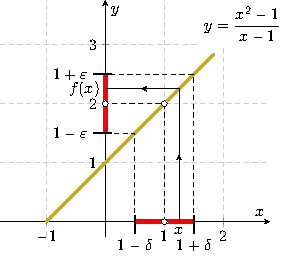
\includegraphics[width=0.45\linewidth]{mai_fig017.pdf}
   \captionof{figure}{K příkladu \ref{MAI:exam028}
   \cite[s.~118]{Brabec1989}
   \label{mai:fig017}}
  \par}
  
  Zvolíme-li libovolně malé okolí bodu \(2\), pak vždy lze najít okolí bodu \(1\) takové, že pro 
  každé \(x \neq 1\) z tohoto okolí bude ležet hodnota \(f(x)\) ve zvoleném okolí čísla \(2\). 
  Ještě jinak formulováno: K libovolně malému \(\varepsilon > 0\) existuje \(\delta > 0\) tak, 
  že pro každé \(x\), pro něž \(0 < \abs{x — 1} \ll \delta\), platí \(\abs{f(x) — 2} < 
  \varepsilon\) (viz obr. \ref{mai:fig017}). O funkci \(f\) s touto vlastností říkáme, že má v bodě 
  \(1\) limitu \(2\) a píšeme symbolicky \(lim_{x \to 1}f(x) = 2\) nebo \(f(x) \rightarrow 2\) pro 
  \(x \rightarrow 1\).
\end{example}
















    %-------------------------------------

    Definičním oborem funkce z příkladu \ref{MAI:exam028} je tedy množina \(\mathcal{D} = \realset 
    — {1}\) (pro \(a = 1\) by ve jmenovateli zlomku byla nula). Grafem funkce je tedy přímka s 
    „vynechaným“ bodem \([1, 2]\) (obr. \ref{mai:fig017}). V bodě \(a = 1\) funkční hodnota není 
    definována. Pokud bychom chtěli rozšířit definiční obor funkce na celou reálnou osu, musíme 
    předepsat, jaké hodnoty má funkce nabývat v bodě \(a = 1\). Původní vzorec, jímž je funkce 
    zadána, výpočet hodnoty \(f(1)\) neumožňuje. Dodatečné zadání funkční hodnoty, její 
    \emph{dodefinování}, můžeme provést zcela libovolně. Zvolme například \(f(1) = 2\). Jiná 
    možnost, jak funkci dodefinovat, je například \(f(1) =-1\). Které číslo je ovšem limitou funkce 
    \(f(x)\) v bodě \(a = 1\)? Je to číslo \(2\), které je v případe \(f(x) = x+1\) její funkční 
    hodnotou? Nebo číslo \(-1\)? A nebo nějaká jiná hodnota? Intuice nám napovídá, že je to číslo 
    \(2\). Když dvojku použijeme pro dodefinování funkce, přetržený graf se „zacelí“. Vidíme, že 
    vezmeme-li dostatečně malý interval proměnné \(x\) v blízkosti bodu \(a=1\) můžeme docílit 
    toho, že všechny odpovídající funkční hodnoty \(f(x)\) budou ležet tak blízko hodnotě \(2\), 
    jak si předem určíme. Skutečně, zkusme docílit toho, aby hodnoty \(f(x)\) ležely v intervalu 
    \((\num{1.99}, \num{2.01})\), tj.
    \begin{equation*}
      \num{1.99} < x + 1 < \num{2.01} \Rightarrow \num{0.99} < x < \num{1.01},\qquad x\neq1.
    \end{equation*}
    Podařilo se. A kdybychom interval \(I(\varepsilon) = (2 - \varepsilon, 2 + \varepsilon)\) 
    funkčních hodnot kolem \(2\) ještě zmenšili, podařilo by se opět najít (o něco menší) interval 
    kolem bodu \(a = 1\) tak, aby pro všechny hodnoty \(x\) v něm (samozřejmě s případnou výjimkou 
    hodnoty \(a =2\)) platilo \(f(x)\in I(\varepsilon)\). A takto bychom mohli \(\varepsilon\) 
    stále zmenšovat. Jak by takový postup dopadl s hodnotou \(-1\), která, jak intuitivně cítíme, 
    limitou funkce v bodě \(a = 1\) není, protože je graf funkce od bodu \([-1,0]\) dost vzdálen? 
    Vezměme třeba interval (\num{-0.5}, \num{0.5}) a hledejme hodnoty \(x\) obdobně jako v 
    předchozím případě. Požadujeme
    \begin{equation*}
      \num{-0.5} < x + 1 < \num{0.5} \Rightarrow \num{-1.5} < x < \num{-0.5}.
    \end{equation*}
    Tento interval vůbec neobsahuje bod \(a = 1\). Dostali jsme se mimo blízkost bodu \(a = 1\).

    %-------------------------------------
      % !TeX spellcheck = cs_CZ
\begin{mathexam}{Najdi limitu funkce \(\varphi(x) = \sqrt[3]{x}\) v bodě \(a = 0\) pomocí
  \eqref{mai:eq037}}{exam029} 
   
  Nechť \(\varphi(x) = \sqrt[3]{x}\), \(a = 0\). Pak \[f(x) = \dfrac{\sqrt[3]{x}}{x}\]. Pro \(x \neq
  0\) je \[f(x) = \frac{1}{\sqrt[3]{x^2}}\]. Jestliže \(x \to 0\), pak hodnoty \(f(x)\) neomezeně
  vzrůstají, protože jmenovatel zlomku se blíží kladnými hodnotami k nule a čitatel je stále roven
  \(1\) (viz obr. \ref{mai:fig018}). Místo rčení \emph{„funkce neomezeně roste“} pro \(x \to 0\)
  říkáme též ]\emph{„funkce se blíží k \(+\infty\)“} pro \(x \to 0\) a píšeme 
  \begin{equation*}
    \lim\limits_{x\to 0} f(x) = +\infty \text{ nebo } f(x)\to +\infty\text{ pro } x\to0.
  \end{equation*}
  Říkáme, že limita funkce \(f\) v bodě \(0\) je rovna \(+\infty\). 
    
  {\centering
  \captionsetup{type=figure}
%   \documentclass[11pt]{standalone}
\usepackage{xltxtra}
\usepackage[usenames,x11names]{xcolor}
\usepackage{tikz}
  \usetikzlibrary{intersections}
  \usetikzlibrary{decorations.markings}
\usepackage{pgfplots}
  \pgfplotsset{compat=newest}
  
\usepackage{amsmath}

\begin{document}
  \begin{tikzpicture}[thick,scale=0.7, 
      every node/.style={transform shape},
      ]
  
  \tikzset{->-/.style={decoration={
    markings,
    mark=at position #1 with {\arrow{stealth}}},postaction={decorate}}}
    
    \begin{axis}[
      xmin = -2.5, xmax = 2.5, ymin = 0, ymax = 3.5,  % osy
      domain = -1:3.5,
      restrict y to domain=0:3.4,
      axis equal image,
      grid = major,   % both
      grid style={line width=.1pt, draw=gray!20},
      major grid style={dashed, line width=.2pt, draw=gray!40},
      clip = true,
      clip mode=individual,
      xtick={-2,-1,1,2,3,4}, % make steps of length 0.2
      ytick={0,1,2,3,4,5}, 
      axis x line = middle,
      axis y line = middle,
      xlabel={\(x\)}, ylabel={\(y\)},
      enlarge y limits={rel=0.07},
      enlarge x limits={rel=0.07},
      ]
  
        \addplot[color=Gold3, samples=100, smooth, ultra thick, unbounded coords=jump,
                 no markers, domain = 0.1:2, name path global=func1] 
           gnuplot{1/((x^2.0)^(1/3.0))};
  
        \addplot[color=Gold3, samples=100, smooth, ultra thick, unbounded coords=jump,
                 no markers, domain = -2:-0.1, name path global=func2] 
           gnuplot{real(1/((x^2.0)^(1/3.0)))};
  
        \node [fill=white] at (rel axis cs: 0.75,0.5) {\(y=\dfrac{1}{\sqrt[3]{x^2}}\)};
  
        \path[name path=line] (-1,1.5) -- (1,1.5); 
            % Intersections points
            \path [name intersections={of=func1 and line,by={P1}}] (P1) node [] {};
  
        \path[name path=line] (-1,1.5) -- (1,1.5); 
            % Intersections points
            \path [name intersections={of=func2 and line,by={Q1}}] (Q1) node [] {};
        
        \draw[black,fill=black] (P1) circle (.3ex);
        \draw[black,fill=black] (Q1) circle (.3ex);
        \path (P1 |- 3,0) -- (P1) -- (P1 -| 0,3) node (X) {};
  
        \draw[thick,red, fill=white] ([shift=(0:1mm)]X) arc (0:180:1mm);
        \draw[->-=.5, dashed]  (P1 |- 3,-0.1)  
          node[below] {\(\delta\)} -- (P1) -- (P1 -| 0,3);
        \draw[->-=.5, dashed]  (Q1 |- -3,-0.1) 
          node[below] {\(\delta\)} -- (Q1) -- (Q1 -| 0,3);
  
        \draw[line width = 2pt, red, line cap=butt] (Q1 |- 3,0) -- (P1 |- 3,0);
        
        \path[name path=line] (-0.7,2.5) -- (0.7,2.5); 
            % Intersections points
            \path [name intersections={of=func1 and line,by={P1}}] (P1) node [] {};
            \draw[->-=.4, dashed, thin,gray] (P1 |- 3,-0.05) node[below] {\(x\)} -- (P1);
            \draw[->-=1, thin, gray] (P1) -- (P1 -| 0,3) node[left, fill=white] {\(f(x)\)};
        \draw[thick,red] (X) node[below left] {\(q\)} -- ++(0cm,2.5cm);
  
       \draw[black,fill=white] (0,0) node[below left] {\(O\)} circle (.4ex);
    \end{axis}
  \end{tikzpicture}
\end{document}
  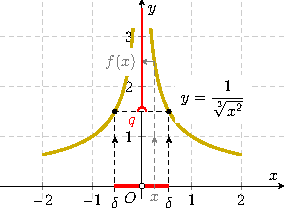
\includegraphics[width=0.8\linewidth]{mai_fig018.pdf}
  \captionof{figure}{K příkladu \ref{MAI:exam029}
  \cite[s.~118]{Brabec1989}
  \label{mai:fig018}}
  \par}
  
  Přesně to znamená toto: Zvolíme-li libovolně velké \(q > 0\), můžeme nalézt \(\delta > 0\) tak, že
  pro každé \(x \neq 0\), pro něž \(\abs{x} < \delta\), platí \(f(x) > q\). 
  
  To lze říci i takto: Zvolíme-li libovolně okolí bodu \(+\infty\), existuje okolí bodu \(0\) tak,
  že pro každé \(x \neq 0\) z tohoto okolí je \(f(x)\) ve zvoleném okolí \(+\infty\) (viz obr.
  \ref{mai:fig018}).
\end{mathexam}
















    %-------------------------------------

    Je třeba říci, že při zkoumání limit funkcí nás nezajímají jen funkce „tvaru“ 
    (\ref{mai:eq037}), i když tento případ je v diferenciálním počtu velmi častý, jak poznáme v 
    kap. \ref{mai:IchapIV}. Někdy nás zajímá i chování funkcí v okolí nevlastních bodů \(-\infty\), 
    \(+\infty\) 

    %-------------------------------------
      % !TeX spellcheck = cs_CZ
\begin{mdframed}[style=mdexam]
  \begin{example}\label{MAI:exam030}
    Je dána funkce \(f: f(x) = \frac{x + 1}{x}\). Sledujme její chování, když hodnoty argumentu
    \(x\) budou vzrůstat nade všechny meze neboli, jak říkáme, \(x\) se bude blížit k \(+\infty\)
    (což zapisujeme \(x \to + \infty\) (viz obr. \ref{mai:fig019}). Můžeme psát \(f(x) = 1 + 1/x\).
    Vzrůstají-li neomezeně hodnoty proměnné \(x\), blíží se hodnoty výrazu \(1/x\) čím dál tím více
    nule, takže funkční hodnoty \(f(x)\) jsou čím dál tím blíže číslu \(1\). V tomto případě píšeme
    \(lim_{x\to+\infty} f(x) = 1\) nebo \(f(x) \to 1\) pro \(x\to +\infty\) a říkáme, že funkce
    \(f\) má v bodě \(+\infty\) limitu rovnou \(1\). Přesně to znamená toto: Zvolíme-li libovolně
    malé \(\varepsilon > 0\), můžeme nalézt \(p > 0\) tak, že pro \(x > p\) platí \(\abs{f(x) - l} <
    \varepsilon\). (Viz obr. \ref{mai:fig019}.) Můžeme to říci i takto: Zvolíme-li libovolně okolí
    bodu \(1\), existuje okolí bodu \(+\infty\) tak, že pro každé \(x\) (konečné) z tohoto okolí je
    \(f(x)\) ve zvoleném okolí bodu \(1\).
    
    {\centering
    \captionsetup{type=figure}
  %   % !TeX spellcheck = cs_CZ

\documentclass[11pt]{standalone}
\usepackage{xltxtra}
\usepackage[usenames,x11names]{xcolor}
\usepackage{tikz}
  \usetikzlibrary{intersections}
  \usetikzlibrary{decorations.markings}
\usepackage{pgfplots}
  \pgfplotsset{compat=newest}
  
\usepackage{amsmath}

\begin{document}
  \begin{tikzpicture}[thick,scale=0.7, 
      every node/.style={transform shape},
      ]
  
  \tikzset{->-/.style={decoration={
    markings,
    mark=at position #1 with {\arrow{stealth}}},postaction={decorate}}}
    
    \begin{axis}[
      xmin = -0.5, xmax = 5.5, ymin = 0, ymax = 4.5,  % osy
      domain =0.2:5,
      restrict y to domain=0:4,
      axis equal image,
      grid = major,   % both
      grid style={line width=.1pt, draw=gray!20},
      major grid style={dashed, line width=.2pt, draw=gray!40},
      clip = true,
      clip mode=individual,
      xtick={1,2,3,4,5}, % make steps of length 0.2
      ytick={0,1,2,3,4}, 
      axis x line = middle,
      axis y line = middle,
      xlabel={$x$}, ylabel={$y$},
      enlarge y limits={rel=0.07},
      enlarge x limits={rel=0.07},
      ]
  
      \addplot[color=Gold3, samples=100, smooth, ultra thick, unbounded coords=jump,
               no markers, domain = 0.1:5, name path global=func1] 
         gnuplot{1+1/x};
  
      \node [fill=white] at (rel axis cs: 0.4,0.75) {\(y=\dfrac{x+1}{x}\)};
  
      \path[name path=line] (0,1.7) -- (3,1.7); 
          % Intersections points
          \path [name intersections={of=func1 and line,by={P1}}] (P1) node [] {};
      
      \draw[black,fill=black] (P1) circle (.3ex);      
      \path (P1 |- 3,-0.1) node [below, fill=white] (X) {p} -- (P1) -- (P1 -| 0,3);
  
      \draw[thick,red, fill=white] ([shift=(90:2.5mm)]X) 
           arc (270:360:1mm) node(Y) {} arc (360:450:1mm);
      \draw[thin] (P1 |- 3,-0.1) -- (P1) -- (P1 -| 0,3);
      \draw[line width = 2pt,red] (Y |- 3,0)  -- ++(3.5,0);
      
   
      \draw[line width = 1pt, black, dashed] (0,1) -- ++(5,0);
      \draw[line width = 3pt, red, line cap=butt] (0,0.3) -- (0,1.7);
      \draw [thick] (-.2, 0.3) node[left] {\(1-\varepsilon\)} -- (0.1, 0.3);
      \draw [thick] (-.2, 1.7) node[left] {\(1+\varepsilon\)} -- (0.1, 1.7 );
  
      \draw[black,fill=white] (0,1) circle (.4ex);

      \path[name path=line] (2.4,0) -- ++(0,2.5); 
          % Intersections points
          \path [name intersections={of=func1 and line,by={P1}}] (P1) node [] {};
          \draw[->-=.4, dashed, gray] (P1 |- 3,-0.05) node[below] {\(x\)} -- (P1);
          \draw[->-=1,  dashed, gray] (P1) -- (P1 -| 0,3) 
            node[left] {\small\(f(x)\)};
            
    \end{axis}
  \end{tikzpicture}
\end{document}
    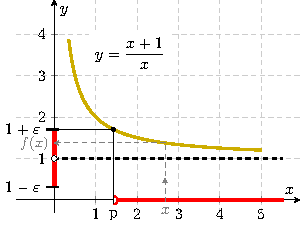
\includegraphics[width=0.45\linewidth]{mai_fig019.pdf}
    \captionof{figure}{K příkladu \ref{MAI:exam030}
    \cite[s.~119]{Brabec1989}
    \label{mai:fig019}}
    \par}
  \end{example}
\end{mdframed}
















    %-------------------------------------
    
    %-------------------------------------
      % !TeX spellcheck = cs_CZ
\begin{mdframed}[style=mdexam]
  \begin{example}\label{MAI:exam031}
    Je dána funkce \(f: f(x) = \frac{x + 1}{x}\). Sledujme její chování, když hodnoty argumentu
    \(x\) budou vzrůstat nade všechny meze neboli, jak říkáme, \(x\) se bude blížit k \(+\infty\)
    (což zapisujeme \(x \to + \infty\) (viz obr. \ref{mai:fig019}). Můžeme psát \(f(x) = 1 + 1/x\).
    Vzrůstají-li neomezeně hodnoty proměnné \(x\), blíží se hodnoty výrazu \(1/x\) čím dál tím více
    nule, takže funkční hodnoty \(f(x)\) jsou čím dál tím blíže číslu \(1\). V tomto případě píšeme
    \(lim_{x\to+\infty}f(x) = 1\) nebo \(f(x) \to 1\) pro \(x\to +\infty\) a říkáme, že funkce \(f\)
    má v bodě \(+\infty\) limitu rovnou \(1\). Přesně to znamená toto: Zvolíme-li libovolně malé
    \(\varepsilon > 0\), můžeme nalézt \(p > 0\) tak, že pro \(x > p\) platí \(\abs{f(x) - l} <
    \varepsilon\). (Viz obr. \ref{mai:fig019}.) Můžeme to říci i takto: Zvolíme-li libovolně okolí
    bodu \(1\), existuje okolí bodu \(+\infty\) tak, že pro každé \(x\) (konečné) z tohoto okolí je
    \(f(x)\) ve zvoleném okolí bodu \(1\).
    
    {\centering
    \captionsetup{type=figure}
  %   % !TeX spellcheck = cs_CZ
% xelatex -enable-write18 -shell-escape mai_fig020.tex
\documentclass[11pt]{standalone}
\usepackage{xltxtra}
\usepackage[usenames,x11names]{xcolor}
\usepackage{tikz}
  \usetikzlibrary{intersections}
  \usetikzlibrary{decorations.markings}
\usepackage{pgfplots}
  \pgfplotsset{compat=newest}
  
\usepackage{amsmath}

\begin{document}
  \begin{tikzpicture}[thick,scale=0.7, 
      every node/.style={transform shape},
      ]
  
  \tikzset{->-/.style={decoration={
    markings,
    mark=at position #1 with {\arrow{stealth}}},postaction={decorate}}}
    
    \begin{axis}[
      xmin = -2, xmax = 3.5, ymin = -2, ymax = 6,  % osy
      domain =-2:8,
      restrict y to domain=-1.5:6,
      axis equal image,
      grid = major,   % both
      grid style={line width=.1pt, draw=gray!20},
      major grid style={dashed, line width=.2pt, draw=gray!40},
      clip = true,
      clip mode=individual,
      xtick={-1,0,1,2,3,4}, % make steps of length 0.2
      ytick={-1,0,1,2,3,4,5,6,7,8}, 
      axis x line = middle,
      axis y line = middle,
      xlabel={$x$}, ylabel={$y$},
      enlarge y limits={rel=0.07},
      enlarge x limits={rel=0.07},
      ]
  
      \addplot[color=Gold3, samples=100, smooth, ultra thick, unbounded coords=jump,
               no markers, domain = -2:2, name path global=func1] 
         gnuplot{x^3};
  
      \node [fill=white] at (rel axis cs: 0.85,0.9) {\(y=x^3\)};
  
      \path[name path=line] (1.5,0) -- (1.5,6); 
          % Intersections points
          \path [name intersections={of=func1 and line,by={P1}}] (P1) node [] {};
          \draw[->-=.4, dashed, gray] (P1 |- 3,-0.05) node[below, fill=white] {\(x\)} -- (P1);
          \draw[->-=1,  dashed, gray] (P1) -- (P1 -| 0,3) 
            node[left=0.5cm, fill=white] {\small\(f(x)\)};
          \draw[dashed, gray] (P1 -| 0,3) + (-0.6cm,0cm) -- (P1 -| 0,3);
      \path[name path=line1] (0,1) -- (2,1); 
          % Intersections points
          \path [name intersections={of=func1 and line1, by={P1}}] (P1) node [] {};    
          \path (P1 |- 3,-0.1) node [below, fill=white] (X) {p} -- (P1) -- (P1 -| 0,3) 
              node[left, fill=white] (Y) {\(q\)};
  
      \draw[thick,red, fill=white] ([shift=(90:2mm)]X) 
           arc (270:360:1mm) node(x1) {} arc (360:450:1mm);
      \draw[dashed] (P1 |- 3,-0.1) -- (P1) -- (P1 -| 0,3);
      \draw[line width = 1pt,red] (x1 |- 3,0)  -- (3,0);
      
      \draw[thick,red] (0,1) -- (0,6);
      \draw[thick,red, fill=white] ([shift=(0:3.3mm)]Y) arc (0:180:1mm);;
    \end{axis}
  \end{tikzpicture}
\end{document}
    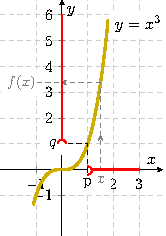
\includegraphics[width=0.35\linewidth]{mai_fig020.pdf}
    \captionof{figure}{K příkladu \ref{MAI:exam031}
    \cite[s.~119]{Brabec1989}
    \label{mai:fig020}}
    \par}
  \end{example}
\end{mdframed}
    %-------------------------------------
    
    V uvedených případech bychom mohli zkoumat i limity funkcí pro \(x \to - \infty\).  Všimněme si 
    ještě, že ve všech případech nebylo nutné, aby funkce \(f\) byla definována v bodě, ke kterému 
    se blíží hodnoty argumentu, ale bylo zapotřebí, aby funkce \(f\) byla definována v bodech 
    libovolně blízkých tomuto bodu. Tomuto požadavku bude vyhověno, jestliže daný bod, v němž 
    zkoumáme limitu, bude \emph{hromadným bodem definičního oboru}. Není ovšem nutné, aby funkce 
    byla definována v celém nějakém \emph{prstencovém okolí uvažovaného bodu}.
    
    Nechť \(a\) je bod, blízko kterého se pohybuje hodnota proměnné \(x\). Pro definici limity je 
    důležitý pojem \textbf{okolí bodu} \(a\) (obr. 2.16). Zvolme kladná čísla \(\delta_1\) a 
    \(\delta_2\). Nazýváme
    
    
      
  %================ Podkapitola: Spojitost funkce ==================================================
  \section{Spojitost funkce}
  
%} % tikzset
%~~~~~~~~~~~~~~~~~~~~~~~~~~~~~~~~~~~~~~~~~~~~~~~~~~~~~~~~~~~~~~~~~~~~~~~~~~~~~~~~~~~~~~~~~~~~~~~~~~
\printbibliography[title={Seznam literatury}, heading=subbibliography]
\addcontentsline{toc}{section}{Seznam literatury}          	
  % !TeX spellcheck = cs_CZ
%{\tikzset{external/prefix={tikz/MAI/}}
% \tikzset{external/figure name/.add={ch10_}{}}
%---------------------------------------------------------------------------------------------------
% file mai1ch03.tex
%---------------------------------------------------------------------------------------------------
\chapter{Kombinatorika, pravděpdobnost, statistika}\label{mai:IchapIII}
\minitoc
  \section{Kombinatorika}\label{mai:IchapIIIsecI}
    \textbf{Kombinatorika} se od všech matematických disciplín, v několika směrech liší. Zatímco v 
    geometrii má každá přímka nekonečnou délku a každý trojúhelník nekonečně mnoho bodů, zatímco v 
    algebře některé rovnice i nerovnice mají nekonečně mnoho řešení a zatímco matematická analýza 
    zkoumá limity posloupností a funkcí, roste-li příslušná proměnná do nekonečna, v kombinatorice 
    se s nekonečnem nesetkáme. Kombinatorika je součástí \textbf{finitní matematiky}, která studuje 
    konečné soubory (množiny a uspořádané \(k\)-tice, \(k\in \mathcal{N}\)). 
    
    Další odlišností je to, že často nemáme možnost ověřit si správnost výsledku, ke kterému jsme 
    při řešení kombinatorické úlohy dospěli, a jsme odkázáni jen na svůj vlastní úsudek. Proto v 
    kombinatorice v míře větší než jinde platí, že „cvičení dělá mistra“. 
    
    V této kapitole je probrána část kombinatoriky, která se zabývá vytvářením skupin z daných 
    prvků a určováním jejich počtu. Jde o klasickou problematiku, která byla řešena již v 17. a 18. 
    století a která je spojena se jmény \emph{B. Pascala}, \emph{P. Fermata}, \emph{J Bernoulliho}, 
    \emph{G. W. Leibnize}  a \emph{L. Eulera}. Dnes představuje kombinatorika rozsáhlou 
    matematickou disciplínu, některé její problémy byly již vyřešeny (problém čtyř barev) mnohé 
    další na své vyřešení čekají. 
    
    A závěrem ještě důležitá poznámka terminologická: přirozeným čísly se v této kapitole rozumějí 
    čísla celá kladná tj. čísla 1, 2, 3, 4, \(\ldots\), nula se tedy mezi přirozená čísla 
    nezahrunuje. \cite[s.~7]{calda2008matematika} 
    
    \subsection{Základní kombinatorická pravidla}
    
    
    \cite[s.~7]{polak1991matematika}
    
  \section{Pravděpodobnost}\label{mai:IchapIIIsecII}
    Slovo pravděpodobnost používáme velmi často. Jaký však je jeho přesný význam? Jsme přesvědčeni, 
    že pravděpodobnost výhry ve sportce je velmi malá. Ani pravděpodobnost, že se vyplní předpověď 
    počasí, nepovažujeme mnohdy za výraznou. Přesto je mezi oběma příklady obrovský kvantitativní 
    rozdíl. Zkusme význam pojmu pravděpodobnost ukázat pomocí konkrétních číselných příkladů.
  
    \begin{itemize}
      \item \textbf{Příklad se střelcem}: Sportovní střelec střílí na terč série \num{100} ran. 
            Předpokládejme, že podmínky při střelbě jsou stále stejné. Stejná je zbraň, terč, 
            vzdálenost, povětrnostní podmínky i momentální zdravotní stav střelce. Při hodnocení 
            střelcova „mistrovství“ někdo řekne, že střelec zasáhne terč s pravděpodobností 
            \num{92}\%. Jak tomu rozumět? Znamená to, že v souboru sérií výstřelů jsou velmi časté 
            ty, v nichž zasáhl střelec terč \num{92}-krát. Samozřejmě, není řídké, že se objeví i 
            série s \num{93} nebo \num{94} zásahy, ale také s \num{91} nebo \num{90}. Vyloučen není 
            ani případ s úspěšností \num{96} či \num{88}, a dokonce i stovku bychom mohli 
            zaznamenat. Situace výrazně odlišné od \num{92} zásahů však budou řídké, a to tím více, 
            čím více se úspěšnost série liší od \num{92} oběma směry.
      \item \textbf{Příklad se zmetky}: Koupíte si výrobek u firmy, o které je známo, že vyrábí 
            zmetky s pravděpodobností 0,16\%? Situaci lze posuzovat obdobně jako úspěšnost střelce. 
            Budeme-li například zkoumat série obsahující 1000 výrobků, bude každá z nich obsahovat 
            „v průměru“ 16\% zmetků. Z příkladu se střelcem již zhruba víme, jak posuzovat slovo v 
            průměru.
    \end{itemize}
    
    V této kapitole se budeme pravděpodobnostmi zabývat podrobněji. Zjistíme, že i když se týkají 
    náhodných jevů, platí i pro ně jisté zákonitosti. V úvodních příkladech jsme si vyložili, jak 
    intuitivně chápat pojem pravděpodobnost. Jednalo se v nich o posouzení průměrné úspěšnosti ve 
    velkém souboru operací či úkonů prováděných za stejných podmínek, šlo tedy o jakousi 
    „průměrnou“ pravděpodobnost. Nyní definujeme pravděpodobnost matematicky.
    
    \subsection{Co se pravdě podobá - definice pravděpodobnosti}
      Pro definici pravděpodobnosti použijeme pojmu \emph{náhodný pokus}, jehož význam si ukážeme 
      na příkladu. Dobrým příkladem náhodných pokusů je třeba házení mincí, hraní kostkou, výběr 
      karet z balíčku, vidíme-li pouze jejich rub, apod. Budeme třeba házet kostkou. Abychom si 
      situaci zbytečně nekomplikovali, budeme předpokládat, že všechny výsledky hodu kostkou 
      (náhodné pokusy) jsou stejně časté, žádný z nich není nijak preferován\footnote{Kostka by 
      tedy měla být homogenní, plocha, na kterou po hodu dopadne, vodorovná, kvalita povrchu všech 
      stěn kostky stejná (žádná stěna by třeba neměla být natřena lepidlem), apod.}. Počet možných 
      výsledků jednotlivého hodu je \(N = 6\) (kostka má \num{6} stěn, na každé je vyznačen odlišný 
      počet ok, tedy \num{1} až \num{6}). Jednotlivé situace, které mohou nastat, nazýváme 
      náhodnými jevy. Náhodným jevem \(A\) tak může být situace \emph{„padne číslo \num{2}“}, jiným 
      náhodným jevem \(B\) situace \emph{„padne číslo dělitelné třemi“}, apod. Počet situací, kdy 
      výsledek hodu lze hodnotit tak, že určitý jev nastal, označíme \(M\). Například pro jev \(A\) 
      \emph{„padne číslo \num{2}“} je \(M(A)= 1\), pro jev \(B\) \emph{„padne číslo dělitelné 
      třemi“} je \(M(B) = 2\) (počet ok \num{3} nebo \num{6}). Můžeme také definovat jev \(O\) 
      \emph{„nepadne žádné číslo“} (\(M(0) = 0\)) nebo jev \(J\) \emph{„padne jakékoli číslo“} 
      (\(M(J) = 6\)).
      
      \begin{definition}
        Pravděpodobností jevu rozumíme podíl
        \begin{equation}\label{mai:eq011}
          p = \frac{M}{N} = \frac{\text{počet případů příznivých}}{\text{počet případů možných}}.
        \end{equation}  
        Počtem případů možných jsme zkráceně nazvali počet všech možných výsledků náhodného 
        pokusu, počtem případů příznivých pak počet všech takových výsledků pokusu, při nichž daný 
        jev nastal.
      \end{definition}
      Je zřejmé, že hodnota pravděpodobnosti jakéhokoli jevu je nezáporná a může nabývat hodnoty 
      nejvýše \num{1}, tj. \(0 <p< 1\). Jev s \emph{nulovou pravděpodobností} se nazývá 
      \textbf{nemožný}, jev s \emph{jednotkovou pravděpodobností} je \textbf{jistý}. V našem 
      příkladu s kostkou tak dostáváme
      \begin{equation*}
        p(A) = \frac{1}{6}, \qquad p(B) = \frac{2}{6} = \frac{1}{3}, \qquad
        p(O) = 0, \qquad p(J) = 1.
      \end{equation*}  

      %--Barevné ponožky----------------------------------------------
      % !TeX spellcheck = cs_CZ
\begin{example}
 \label{mai:exam006}
  \textbf{Barevné ponožky}:\newline\small
  V zásuvce jsou ponožky tří barev. Červené (\textbf{Č}), zelené (\textbf{Z}) a modré (\textbf{M}). 
  Je jich tam od každé barvy hodně. Student jde na schůzku a chce si vzít čisté ponožky. Náhle 
  zhasne světlo. Student vytáhne potmě dvě ponožky. Jaká je pravděpodobnost, že ponožky budou mít 
  stejnou barvu? Vyjmenujme případy, které mohou při vytažení dvou ponožek nastat: (\textbf{Č+Č}), 
  (\textbf{Č+Z}), (\textbf{Z+Č}), (\textbf{Č+M}), (\textbf{M+Č}), (\textbf{Z+Z}), (\textbf{Z+M}), 
  (\textbf{M+Z}), (\textbf{M+M}). Je tedy \(n = 9\). Příznivé situace jsou tří, (\textbf{Č+Č}), 
  (\textbf{Z+Z}), (\textbf{M+M}). Pravděpodobnost je tedy 1/3. (Převzato z 
  \cite[s.~200]{Musilova2009MA1}) 
\normalsize
\end{example}
      %---------------------------------------------------------------
    \subsection{Cifry, kostky, karty - kombinatorické opakování}
      Příklad s ponožkami byl velmi jednoduchý. Podařilo se nám vyjmenovat všechny případy možné i 
      všechny případy příznivé, neboť obojího bylo docela málo. Daleko běžnější jsou však situace, 
      kdy výčet případů není schůdný. A tehdy potřebujeme \textbf{kombinatoriku}.
      
      Nechť \(\mathcal{M}\) je \(n\)-prvková množina, z níž budeme provádět výběry \(k\) prvků 
      podle určitých pravidel. Prvky množiny \(\mathcal{M}\) nemusíme nijak konkretizovat. Abychom 
      si však o výběrech a pravidlech pro jejich tvorbu dokázali udělat nějakou názornou představu, 
      je taková konkretizace vhodná. Prvky množiny \(\mathcal{M}\): mohou být třeba žáci ve třídě, 
      barvy, hrací karty, apod. Výběry mohou představovat třeba družstva pro odbíjenou, signály 
      tvořené barevnými praporky, možnosti rozdání karet při mariáši, apod. Jednotlivé typy výběrů 
      získaly své názvy právě na základě pravidel stanovených pro jejich vytváření. Rozhodující 
      jsou dvě základní kritéria:
      \begin{itemize}\addtolength{\itemsep}{-0.5\baselineskip}
        \item Je pro tvorbu výběru podstatné pořadí prvků ve výběru či nikoliv?
        \item Mohou se prvky ve výběru opakovat či nikoliv?
      \end{itemize}
      
      Typy výběrů shrnuje následující diagram:
      \begin{figure}[ht!] %\ref{mai:fig021}
        \centering
        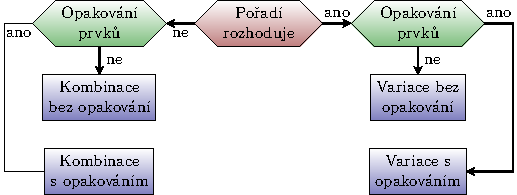
\includegraphics[width=0.7\linewidth]{mai_fig021.pdf}
        \caption{Typy výběrů. \cite[s.~201]{Musilova2009MA1}}
        \label{mai:fig021}
      \end{figure}

      Představuje-li daný výběr například volejbalové družstvo osmi děvčat (šest hráček a dvě 
      náhradnice), které bude reprezentovat v soutěži třídu osmou bé, do níž chodí \num{25} děvčat 
      a \num{18} chlapců, jedná se o výběr \(k - 8\) prvků z počtu \(n = 25\) prvků. Chlapce nelze 
      postavit do družstva volejbalistek. Každý výběr možného družstva bude představovat 
      \emph{kombinaci bez opakování}, neboť pořadí hráček nehraje roli a třeba Aničku Novákovou 
      máme ve třídě jen jednu. Budeme-li však chtít vytvářet z deseti cifer \(0, 1, \ldots, 9\) 
      trojciferná čísla, pak tyto výběry tří prvků z deseti (\(k = 3\), \(n = 10\)) jsou 
      \emph{variacemi s opakováním}. Čísla \num{125}, \num{512}, \num{251}, \num{215}, \num{521} a 
      \num{152} jsou totiž různá, a například \num{222} je také trojciferné číslo. Kombinace s 
      opakováním bychom mohli vytvářet třeba i při výběru různobarevných ponožek ze zásuvky a 
      konečně \emph{variacemi bez opakování} by mohly být dejme tomu trojbarevné signály (\(k = 
      3\)) tvořené trojicemi barevných hadříků vybíraných z \(n\) barev (pro \(n = 3\) třeba zrovna 
      z těch ponožek). Nyní bychom však rádi věděli, jak pro zadané hodnoty \(n\) a \(k\) určit 
      počet všech možných výběrů předepsaného typu. Ukážeme si to na příkladech.

      %--Šance milion-------------------------------------------------
      % !TeX spellcheck = cs_CZ
\begin{mdframed}[style=mdexam]
  \begin{example}\label{mai:exam007}
    \textbf{Šance milion}:\newline
    „Znáte nějakou jinou hru, kde můžete denně vyhrát milion?“ Tento nebo jiný, obdobně nepříliš
    vtipný reklamní slogan propaguje v televizi hru, jejímž cílem je uhodnout šestici tažených cifer
    ve správném pořadí. (Hru raději nehrajte, pravděpodobnost výhry je mizivá.) Tah se provádí
    následovně: V každém ze šesti bubnů, očíslovaných pořadovými čísly \num{1} až \num{6}, je
    připraveno deset míčků opatřených ciframi \(0, 1, \ldots, 9\). Z prvního bubnu se náhodně
    vylosuje jedna cifra (deset možností). Poté se náhodně vylosuje jedna cifra z druhého bubnu
    (opět deset možností). Možností vzniku uspořádané dvojice cifer (jedna cifra z prvního a druhá z
    druhého bubnu) je již sto (každou možnost výsledku u prvního bubnu lze kombinovat s každou
    možností výsledku z druhého bubnu). Losování pokračuje u třetího, čtvrtého, pátého a šestého
    bubnu. Celkový počet možností je \num{1e6}, tedy \textbf{milion}. (Šance získat výhru, tedy
    vyhrát milion, je ovšem pouze jedna milióntina, neboť z milionu možností je pouze jedna skutečně
    tažena.) 
  \end{example}
\end{mdframed}
      %---------------------------------------------------------------
      
      Zobecněním předchozího příkladu získáváme vzorec pro počet \textbf{variací s opakováním} 
      \emph{k}-té třídy z \(n\) prvků. Při tahu totiž záleží na pořadí bubnů a každý buben obsahuje 
      všechny cifry. Výsledky tahů z jednotlivých bubnů se tedy mohou opakovat. Pokud by bubnů bylo 
      \(k\) a v každém \(n\) různých cifer, dostali bychom pro \textbf{variace s opakováním 
      \(k\)-té třídy z \(n\) prvků} celkový počet
      \begin{equation}\label{mai:eq007}
        \boxed{V_k' = n^k}\, .
      \end{equation}

      %--Modifikovaná šance milion------------------------------------
      % !TeX spellcheck = cs_CZ
\begin{example}\label{mai:exam008}
  \textbf{Modifikovaná šance milion}:\newline
  Představme si hru z předchozího příkladu upravenou takto: K dispozici bude jen jeden buben s 
  ciframi \(0, 1, \ldots, 9\), každá cifra je v bubnu obsažena pouze jednou. Opět máme losovat 
  uspořádanou \textbf{šestici cifer}. Nyní se však jedná o \textbf{variace šesté třídy z deseti 
  prvků bez opakování}. S jediným bubnem musíme totiž provést šest losování, přičemž při každém 
  losování ubude z bubnu jedna cifra. Při prvním tahu je deset možností, při druhém již jen devět, 
  atd., při šestém již pouze pět možností. Celkem je tedy \(10 \cdot 9 \cdots 5 = \num{151200}\) 
  možností.
\end{example}
      %---------------------------------------------------------------
      
      Uvážíme-li, že v předchozím příkladu je \(n = 10\) a \(k = 6\), dostáváme pro \textbf{počet 
      variací bez opakování \(k\)-té třídy z \(n\) prvků} obecný vztah
      \begin{align}
        V_k(n) &= n(n-1)(n-2)\cdots(n-k+1)  \nonumber \\
        \shortintertext{neboli}
        V_k(n) &= \frac{n!}{(n-k)!}\, .    \label{mai:eq008}
      \end{align}
      Poznamenejme, že \(n!\) značí \textbf{faktoriál}, \(n! = n(n - 1)\cdots 3 \cdot 2 \cdot 1\). 
      Pro nulu definujeme \(0! = 1\). Je zřejmé, že při vytváření variací bez opakování musí být 
      \(k\leqq n\). Variace bez opakování \(n\)-té třídy z \(n\) prvků se nazývají 
      \textbf{permutace}. Každá z nich představuje určité uspořádání těchto \(n\) prvků. Platí
      \begin{equation}\label{mai:eq009}
        \boxed{P(n) = V_n(n) = n!}\, .
      \end{equation}
      
      Nyní odvodíme vzorec pro počet \textbf{kombinací \(k\)-té třídy z \(n\) prvků bez opakování}. 
      Již jsme si řekli, že \emph{kombinací} rozumíme takový výběr z celkového počtu \(n\) prvků, 
      který obsahuje určitých \(k\) prvků nezávisle na jejich pořadí. Představme si, že máme k 
      dispozici všechny variace bez opakování \(k\)-té třídy ze zmíněných \(n\) prvků. Vezměme 
      kteroukoli z nich. Soubor všech variací \(k\)-té třídy z \(n\) prvků však obsahuje i další 
      variace, lišící se od té naší jen pořadím prvků. Celkem je takových variací (i s tou první) 
      \(k!\) a z hlediska kombinací představují totéž. Soubor variací se tak rozpadá na podsoubory, 
      z nichž každý obsahuje \(k!\) variací lišících se navzájem pouze pořadím prvků. Každý z 
      těchto podsouborů představuje však jedinou kombinaci. Počet kombinací \(k\)-té třídy z \(n\) 
      prvků bez opakování je tedy
      \begin{equation}\label{mai:eq010}
        \boxed{C(k) = \frac{V_k(n)}{P(k)} = \frac{n!}{(n-k)!\,k!} = 
               \begin{pmatrix}
                n \\
                k
               \end{pmatrix}}\, .
      \end{equation}
      
      Pro odvození vzorce pro \textbf{kombinace s opakováním} použijeme opět příkladu.
      %--Kuličky v přihrádkách----------------------------------------
      % !TeX spellcheck = cs_CZ
\begin{mathexam}{Kuličky v přihrádkách}{exam009}
  Máme kuličky \(n\) různých barev, v každé barvě máme tolik kuliček, kolik bude potřeba. Naším
  úkolem je vytvářet výběry \(k\) kuliček. Na \textbf{pořadí barev nezáleží}, kuliček jedné barvy
  může být ve výběru libovolný počet \(0\leqq s \leqq k\). Výběry budeme vytvářet tak, že budeme
  kuličky dávat do \(n\) přihrádek, z nichž každá bude vyhrazena pro určitou barvu. Pokud tedy v
  daném výběru zrovna nebude třeba modrá kulička, bude přihrádka vyhrazená pro modrou barvu prázdná.
  Budou-li v daném výběru právě tři červené kuličky, budou umístěny v přihrádce vyhrazené pro
  červenou barvu. Vidíme, že pokud konkrétním přihrádkám přisoudíme konkrétní barvy, samotné kuličky
  by již barevné být nemusely, stačily by třeba kuličky skleněné, bezbarvé. Zůstane-li například
  přihrádka pro modrou barvu prázdná, víme, že daný výběr neobsahuje modrou barvu. Budou-li v
  přihrádce pro červenou barvu tři (bezbarvé) kuličky, víme, že daný výběr obsahuje červenou barvu
  třikrát. Příklad takové situace ukazuje následující schéma:
  
  {\centering
    \luafigure[0.9]{mai_fig033.pdf}
    \par}

  Náš úkol můžeme přeformulovat takto: Je třeba rozmístit \(k\) kuliček do \(n\) přihrádek. V každé
  přihrádce může být obecně \(s\) kuliček, kde \(0\leqq s \leqq k\), přitom celkový počet kuliček
  musí být samozřejmě stále \(k\). Můžeme si představit, že \(k\) kuliček máme položených v řadě na
  polici mezi dvěma pevnými stěnami (krajní svislé čáry v předchozím schématu) a různé způsoby
  rozmístění kuliček do přihrádek provádíme přemísťováním pohyblivých přepážek. Kdybychom například
  v předchozím schématu přesunuli druhou svislou čáru, počítáno zleva, až za první kuličku v
  přihrádce na červenou barvu, dostaneme uspořádání, při němž je v přihrádce na modrou barvu jedna
  kulička a v přihrádce na červenou barvu dvě kuličky. Tedy takto:

  {\centering
    \luafigure[0.9]{mai_fig034.pdf}
  \par}

  Mezi dvěma krajními pevnými stěnami máme tedy k dispozici \(k\) pozic pro kuličky a \((n - 1)\)
  pozic pro pohyblivé přepážky. Celkem tedy \((n + k - 1)\) pozic, na které můžeme libovolně
  rozmísťovat \(k\) kuliček a \((n - 1)\) přepážek. Do těchto \((n + k - 1)\) pozic můžeme umístit
  \(k\) kuliček \(C_k'(n)\) způsoby, kde
  \begin{equation}\label{MAI:eq011}
    \boxed{C_k'(n) =  \binom{n + k - 1}{k} = \binom{n + k - 1}{n -1}}\, .
  \end{equation}
  Na zbylé pozice již musíme umístit přepážky. Nebo naopak, nejprve umístíme \((n - 1)\) přepážek a
  potom kuličky. Výsledek je stejný, jak je vidět z předchozího vzorce. Protože jsme vytváření
  kombinací s opakováním \(k\)-té třídy z \(n\) prvků převedli na úlohu o rozmísťování kuliček do
  přihrádek, udává získaný vzorec právě počet takových kombinací. Aby měl vzorec smysl, musí platit
  \(n + k - 1 \geqq k\), tedy \(n \geqq 1\).

  Komu nevyhovuje představa kuliček v přihrádkách a má raději čísla, může uvažovat následovně: Tak
  jako je každé číslo v desítkové soustavě zapsáno pomocí cifer \(0, 1, 2, \ldots , 8, 9\), je k
  jeho zápisu ve dvojkové soustavě potřeba pouze dvou cifer, nuly a jedničky. Představme si nyní
  přepážku jako jedničku a kuličku jako nulu. Náš úkol zjistit počet všech možných způsobů rozdělení
  \(k\) kuliček do \(n\) přihrádek, ohraničených \((n+1)\) přepážkami, můžeme převést na
  ekvivalentní problém: Kolik dokážeme najít čísel, která jsou ve dvojkové soustavě zapsána právě
  \(k\) nulami a \((n + 1)\) jedničkami, požadujeme-li, aby první i poslední cifrou byla jednička?
  Odpověď je jednoduchá. Máme k dispozici \((n+k+1)\) pozic pro cifry. První a poslední pozice jsou
  pevně obsazeny jedničkami, volných pozic je tedy pouze \((n + k - 1)\). Počet všech různých
  způsobů, kterými na \(k\) z těchto pozic můžeme umístit nuly, je roven počtu kombinací \(k\)-té
  třídy z \((n + k - 1)\) prvků. Na zbylé pozice již musíme umístit jedničky. Komplementárně,
  budeme-li hledat počet všech možných způsobů, jak na \((n-1)\) pozic umístit jedničky, dostaneme
  shodný výsledek, v souhlasu se vzorcem (\ref{mai:eq010}).
\end{mathexam}
      %---------------------------------------------------------------
      
      %--Obsazování kvantových stavů----------------------------------
      % !TeX spellcheck = cs_CZ
\begin{example}\label{mai:exam010}
  \textbf{Obsazování kvantových stavů}:\newline\small
  Úloha o kuličkách a přihrádkách má přímou aplikaci v \textbf{kvantové fyzice}. Představme si, že 
  fyzikální soustava je tvořena \(k\) částicemi. Každá částice se nachází v určitém stavu, v němž 
  jí můžeme přisoudit fyzikální charakteristiky, které jsou s tímto stavem spojeny (třeba energii, 
  moment hybnosti, apod.). Jednotlivé stavy jsou pak rozlišitelné právě pomocí těchto 
  charakteristik. Dejme tomu, že přípustných stavů je \(n \geqq 1\). Problémem kvantové fyziky je 
  to, že kvantové částice jsou nerozlišitelné. Nepoznáme jednu od druhé. Je to stejné, jako bychom 
  měli \(k\) naprosto stejně vypadajících kuliček, které nemáme nijak očíslovány. Záměna dvou 
  částic (nerozlišitelných kuliček) se nepozná, nevede tedy ke změně stavu fyzikální soustavy. Pro 
  hodnoty fyzikálních charakteristik soustavy jako celku je tedy důležité jen to, kolik částic je v 
  každém z přípustných stavů. Musíme se tedy zajímat o to, kolika způsoby lze našich \(k\) 
  \textbf{nerozlišitelných částic} (kuliček) umístit do \(n\) \textbf{stavů} (přihrádek). Kvantové 
  částice jsou však dvojího druhu, \textbf{fermiony} (například elektrony, neutrony, protony, jádra 
  s lichým počtem nukleonů) a \textbf{bosony} (například fotony, mezony, jádra se sudým počtem 
  nukleonů). Rozdíl mezi nimi je ten, že bosony se „dobře snášejí“, a proto jich může být v jednom 
  stavu i více. 
  \begin{itemize}\addtolength{\itemsep}{-0.5\baselineskip}
    \item Počet možností, jak rozmístit \(k\) \textbf{bosonů} po \(n\) stavech je tedy
          \begin{equation*}
            N_{\text{boson}} = 
              \begin{pmatrix}
                n + k - 1 \\
                    k
               \end{pmatrix}
          \end{equation*}
    \item S \textbf{fermiony} je tomu jinak. \textbf{Pauliho vylučovací princip} jim zakazuje, 
          aby v daném stavu byl více než jeden fermion. Stav může být buď prázdný, nebo obsazen 
          jedním fermionem. V takovém případě musí být \(n \geqq k\) a v každé přihrádce může být 
          nejvýše jedna kulička. Situace tak odpovídá \textbf{kombinacím bez opakování \(k\)-té 
          třídy z \(n\) prvků}, tj.
          \begin{equation*}
            N_{\text{fermion}} = 
              \begin{pmatrix}
                n  \\
                k
              \end{pmatrix}
          \end{equation*}
  \end{itemize}
\normalsize
\end{example}
      %---------------------------------------------------------------
      
      Získané kombinatorické vzorce nyní použijeme při řešení základních úloh o pravděpodobnostech. 
      V každé úloze bude důležité
      \begin{itemize}
        \item definovat jev \(A\), jehož pravděpodobnost počítáme,
        \item určit počet \(N\) případů možných, tj. počet všech možných výsledků pokusu, při 
              kterém sledujeme, zda jev \(A\) nastal či nenastal,
        \item určit počet \(M\) případů příznivých, tj. počet těch výsledků daného pokusu, při 
              kterých jev \(A\) nastal.
      \end{itemize}

      %--Výhra ve sportce---	----------------------------------------
      % !TeX spellcheck = cs_CZ
\wikitextrule
\begin{example}\label{mai:exam052}
  \textbf{Výhra ve sportce}\newline\small
  Jaká je pravděpodobnost hlavní výhry ve sportce? Všichni víme, že malá, ale máme představu, jak 
  malé toto číslo je? Při sportce se losuje \(k = 6\) čísel a jedno dodatkové z celkového počtu \(n 
  = 49\) čísel. (Dříve byla čísla spojena s názvy sportů, odtud název „sportka“ .) Na pořadí čísel 
  ve výběru nezáleží, vytažené číslo se do hry nevrací. Jde tedy o \textbf{kombinace bez 
  opakování}. Hlavní výhra požaduje uhodnout všech \num{6} tažených čísel. Jev \(A\) je tedy 
  definován takto:
  
  \begin{itemize}
    \item Jev \(A\): Bude taženo právě oněch \num{6} čísel, která jsem vsadil.
          Počet možností, které při tahu sportky mohou nastat (počet případů možných), je \(N = 
          \begin{pmatrix} n \\ k\end{pmatrix} =  \begin{pmatrix} 49 \\ 6 \end{pmatrix} \). Hlavní 
          výhru představuje jediná kombinace, počet příznivých případů je proto \(M = 1\). 
          Pravděpodobnost hlavní výhry ve sportce, tj. pravděpodobnost jevu \(A\), je
          \begin{equation*}
            p(A) = \dfrac{M}{N} = \dfrac{1}{\begin{pmatrix} 49 \\ 6 \end{pmatrix}} 
                 = \dfrac{43!6!}{49!} = \dfrac{720}{49\cdot48\cdot47\cdot46\cdot45\cdot44} \simeq 
                 \num{7e-8}
                 = \SI{7e-6}{\percent}
          \end{equation*}
          Pravděpodobnost hlavní výhry je velmi malá, sedm milióntin procenta. 
    \item A o kolik lepší to bude s pravděpodobností některé z vedlejších výher? Tak třeba pátá 
          cena znamená, že je nutné ze šesti tažených čísel uhodnout libovolné tři. Jev \(A\) je 
          tedy: Ze šesti čísel, která jsme vsadili, budou v tažené kombinaci obsažena právě tři 
          libovolná z nich. Počet \(N\) zůstává stejný jako v předchozí části úlohy. Je třeba jen 
          určit \(M\). Každý příznivý případ vzniká tak, že trojice správných čísel (výběry tří ze 
          šesti) je doplněna trojicí chybných čísel (výběry tří ze čtyřiceti tří). Tedy \(M = 
          \begin{pmatrix}6 \\ 3\end{pmatrix}\begin{pmatrix} 49 - 6 \\ 3\end{pmatrix} =  
          \begin{pmatrix} 6 \\ 3\end{pmatrix}\begin{pmatrix} 43 \\ 3 \end{pmatrix}\),
          \begin{align*}
            p(A) &= \dfrac{M}{N} 
                  = \dfrac{\begin{pmatrix} 6 \\ 3\end{pmatrix}
                           \begin{pmatrix} 43 \\ 3 \end{pmatrix}}
                          {\begin{pmatrix} 49 \\ 6\end{pmatrix} }                
                  =\left(\dfrac{6!}{3!\cdot3!}\right)\left(\dfrac{43!}{40!\cdot3!}\right)
                   \left(\dfrac{43!6!}{49!}\right)                                            \\
                 &=\dfrac{120\cdot43\cdot42\cdot41\cdot720}
                         {49\cdot48\cdot47\cdot46\cdot45\cdot44\cdot36} 
                  \simeq\num{0.018}.
          \end{align*}
          Tato pravděpodobnost již zanedbatelná není, na rozdíl od finanční částky, jíž bývá 
          ohodnocena pátá cena. Sázení sportky může domácímu rozpočtu spíše ublížit.
    \item Třetí, resp. čtvrtá cena jsou, podobně jako první a pátá, definovány velmi jednoduše. Je 
          třeba uhodnout pět, resp. čtyři ze šesti tažených čísel. V případě druhé ceny hraje roli
          dodatkové číslo. Druhou cenu získává ten, kdo uhodl pět ze šesti čísel vylosovaných v 
          prvním tahu a ještě navíc číslo dodatkové, které se losuje ze zbylých \num{43} čísel, jež 
          zůstala po prvním tahu v osudí. Jev \(A\) je tedy definován takto:
          
          Ze šesti čísel, která jsem vsadil, bude při prvním tahu vylosováno libovolných pět a v 
          druhém tahu bude vylosováno právě to dodatkové číslo, které jsem vsadil. Počet případů 
          příznivých je pouze \(M = \begin{pmatrix}6 \\ 5\end{pmatrix}\), neboť šestým číslem 
          nemůže být libovolné ze \num{43} čísel, která nebyla v prvním tahu vylosována, ale 
          musí to být právě číslo dodatkové. Pravděpodobnost jevu \(A\) je
          \begin{equation*}
            p(A)  = \dfrac{M}{N} 
                  = \dfrac{\begin{pmatrix} 6  \\ 5\end{pmatrix}}
                          {\begin{pmatrix} 49 \\ 6\end{pmatrix}}
                  \simeq\num{4.2e-17}.
          \end{equation*}
          
          Pokud bychom jako jev \(A\) označili výhru jakékoliv ceny, dostaneme
          \begin{align*}
            M &= \sum_{6}^{k=3}\begin{pmatrix} 6  \\   k  \end{pmatrix}
                               \begin{pmatrix} 43 \\ 6 - k\end{pmatrix}  +
                               \begin{pmatrix} 6  \\   5  \end{pmatrix}                      \\
              &= \begin{pmatrix} 6 \\ 3\end{pmatrix}\begin{pmatrix} 43 \\ 3\end{pmatrix} +
                 \begin{pmatrix} 6 \\ 4\end{pmatrix}\begin{pmatrix} 43 \\ 2\end{pmatrix} +
                 \begin{pmatrix} 6 \\ 5\end{pmatrix}\begin{pmatrix} 43 \\ 1\end{pmatrix} +
                 \begin{pmatrix} 6 \\ 6\end{pmatrix}\begin{pmatrix} 43 \\ 0\end{pmatrix} +
                 \begin{pmatrix} 6 \\ 5\end{pmatrix},                                        \\
           p(A) &= \dfrac{\begin{pmatrix}  6 \\ 3\end{pmatrix}
                          \begin{pmatrix} 43 \\ 3\end{pmatrix}  +
                          \begin{pmatrix}  6 \\ 4\end{pmatrix}
                          \begin{pmatrix} 43 \\ 2\end{pmatrix}  +
                          \begin{pmatrix}  6 \\ 5\end{pmatrix}
                          \begin{pmatrix} 43 \\ 1\end{pmatrix}  +
                          \begin{pmatrix}  6 \\ 6\end{pmatrix}
                          \begin{pmatrix} 43 \\ 0\end{pmatrix}  +
                          \begin{pmatrix}  6 \\ 5\end{pmatrix}}
                         {\begin{pmatrix} 49 \\ 6\end{pmatrix}} =\simeq\num{0.019}.
          \end{align*}
          Všimněte si, že tento výsledek je roven součtu pravděpodobností výhry páté, čtvrté, 
          třetí, druhé a hlavní ceny. Později si tento závěr ještě připomeneme.
  \end{itemize}  
  \normalsize
\end{example}
      %---------------------------------------------------------------

      %--Losování karet-----------------------------------------------
      % !TeX spellcheck = cs_CZ
\wikitextrule
\begin{example}\label{mai:exam053}
  \textbf{Losování karet}\newline\small
    Máme karetní hru mariáš, která obsahuje celkem \num{32} karet osmi hodnot \num{7}, \num{8}, 
    \num{9}, \num{10}, J (kluk), Q (dáma), K (král), A (eso), každá hodnota je ve čtyřech barvách, 
    červené barvy jsou \(\heartsuit\) (srdce) a \(\lozenge\) (kára), černé barvy jsou \(\spadesuit\)
    (piky) a \(\clubsuit\) (kříže). Jaká je pravděpodobnost, že při náhodném vylosování deseti 
    karet budou 
    mezi nimi:
    \begin{enumerate}[label=\Alph*]
      \item právě dvě esa,
      \item alespoň dvě esa,
      \item nejvýše dvě esa,
      \item alespoň šest karet stejné barvy,
      \item právě dvě dámy a alespoň jeden kluk,
      \item právě dvě dámy nebo alespoň jeden kluk?
    \end{enumerate}

    Písmena (A) až (F) představují různé části úlohy a také zároveň definují jevy, jejichž 
    pravděpodobnost počítáme. Jedná se opět o kombinace. Nezáleží totiž na pořadí, v jakém karty 
    vytahujeme. Důležité je jen to, zda jsou vyjmenované karty ve výběru obsaženy. Počet možných 
    výsledků náhodného vylosování deseti karet z dvaatřiceti, tj. počet případů možných, je pro 
    všechny části úlohy stejný,
    \begin{equation*}
      N = \begin{pmatrix} 32 \\ 10\end{pmatrix} 
        = \dfrac{32\cdot31\cdots24\cdot23}{10\cdot9\cdots2\cdot1} = \num{64512240}.
    \end{equation*}
    
    Počítejme nyní případy příznivé pro jednotlivé jevy \(A\) až \(F\) a pravděpodobnosti těchto 
    jevů:
    \begin{equation*}
      M(A) = \begin{pmatrix} 4 \\ 2\end{pmatrix}\begin{pmatrix} 32 - 4 \\ 10 - 2\end{pmatrix}
           = \begin{pmatrix} 4 \\ 2\end{pmatrix}\begin{pmatrix} 28 \\ 8\end{pmatrix}
           = 6\cdot\dfrac{28\cdot27\cdots1}{8\cdot7\cdots2\cdot1} = \num{18648630}.
    \end{equation*}
    Jak jsme k tomuto výsledku došli? Příznivý pro daný jev je každý výběr, v němž jsou obsažena 
    právě dvě esa (libovolných barev) a žádná další esa (význam slova „právě“). Počet výběrů dvou 
    es z celkového počtu čtyř es je \(C_2(4)\), počet výběrů dalších libovolných osmi karet ze 
    zbývající části hry, která vznikne po odstranění es (nechceme, aby v příznivém výběru byla 
    další esa), je \(C_{(10-2)}(32 - 4) = C_8(28)\). Každý výběr dvojice es lze kombinovat s každým 
    výběrem zbývajících osmi karet ze zbytku hry, tj. \(M(A) = C_2(4)\cdot C_8(28)\). A to je právě
    náš předchozí výsledek. Potom:
    \begin{equation*}
      p(A) = \dfrac{M(A)}{N} 
           = \dfrac{\begin{pmatrix} 4 \\ 2\end{pmatrix}\begin{pmatrix} 28 \\ 8\end{pmatrix}}
                   {\begin{pmatrix} 32 \\ 10\end{pmatrix}}
           = \dfrac{\num{18648630}}{\num{64512240}} \simeq \num{0.29}
    \end{equation*}
    
    Aby nastal jev \(B\), požadujeme, aby v náhodném výběru deseti karet z dvaatřiceti byla alespoň 
    dvě esa. To znamená, že výběr považujeme za příznivý, obsahuje-li dvě esa libovolné barvy a osm 
    libovolných karet jiné hodnoty, nebo obsahuje tři esa libovolné barvy a sedm libovolných karet 
    jiné hodnoty, nebo obsahuje všechna čtyři esa a šest libovolných karet jiné hodnoty, \(k\) es 
    (pro \(k = 2, 3, 4\)) můžeme ze čtyř es vybrat \(\begin{pmatrix} 4 \\ k\end{pmatrix}\) způsoby.
    \(10 - k\) karet jiné hodnoty pak musíme vybírat pouze z \num{28} karet (esa je nutno 
    odstranit, aby bylo zaručeno, že „doplňkové“ karty budou mít jinou hodnotu než eso). Výběr 
    zbývajících karet lze učinit \(\begin{pmatrix} 28 \\ 10 - k\end{pmatrix}\) způsoby. Nakonec 
    tedy dostáváme
    \begin{align*}
      M(B) &=  \begin{pmatrix} 4 \\ 2\end{pmatrix}\begin{pmatrix} 28 \\ 8\end{pmatrix}
              +\begin{pmatrix} 4 \\ 3\end{pmatrix}\begin{pmatrix} 28 \\ 7\end{pmatrix}
              +\begin{pmatrix} 4 \\ 4\end{pmatrix}\begin{pmatrix} 28 \\ 6\end{pmatrix}         \\
           &=  6\cdot\dfrac{28\cdot27\cdots22\cdot21}{8\cdot7\cdots2\cdot1}
              +4\cdot\dfrac{28\cdot27\cdots23\cdot22}{7\cdot6\cdots2\cdot1}
              +1\cdot\dfrac{28\cdot27\cdots24\cdot23}{6\cdot5\cdots2\cdot1} = \num{23761530},  \\
      P(B) &= \dfrac{M(B)}{N} = \dfrac{\num{23761530}}{\num{64512240}} \simeq\num{0.37}.
    \end{align*}
    Pozn.: Někomu se předchozí výpočet může zdát příliš složitý. Nelze jej nějak zjednodušit? Co 
    kdybychom uvažovali třeba takto: Výběr dvou es již zajistí splnění požadavku. Doplňkové karty 
    tedy již pak můžeme vybírat ze třiceti karet - nebudeme tedy odstraňovat esa, protože budou-li 
    vybrána mezi doplňkovými kartami, požadavek „alespoň dvou es ve výběru“ to nenaruší. Při takové 
    interpretaci bychom dostali
    \begin{equation*}
      M(B) = \begin{pmatrix} 4 \\ 2\end{pmatrix}\begin{pmatrix} 30 \\ 8\end{pmatrix}   
           = 6\cdot\dfrac{30\cdot29\cdots24\cdot23}{8\cdot7\cdots2\cdot1}
           = \num{35117550}.
    \end{equation*}
    Vidíme, že vyšlo číslo vyšší než při předchozí úvaze. Co je tedy správně? Správně je první 
    úvaha vedoucí k nižšímu počtu příznivých případů. Při druhé úvaze jsme některé případy 
    započetli vícekrát. Zkuste přijít na to, jak se to stalo. V každém případě vidíme, že 
    kombinatorické úvahy, ať již vypadají jakkoli jednoduše, mohou být zrádné a je třeba dát si na 
    ně pozor. 
    
    Jev \(C\) podle zadání nastane, obsahuje-li náhodný výběr deseti karet nejvýše dvě esa. Znamená 
    to, že výběr je příznivý, neobsahuje-li žádné eso a obsahuje deset karet jiné hodnoty, nebo 
    obsahuje-li jedno eso a devět karet jiné hodnoty, nebo obsahuje-li dvě esa a osm karet jiné 
    hodnoty. Počet \(M(C)\) určíme analogicky jako \(M(B)\), ale pro \(k= 0, 1, 2\):
    \begin{align*}
      M(C) &=  \begin{pmatrix} 4 \\ 0\end{pmatrix}\begin{pmatrix} 28 \\ 10\end{pmatrix}
              +\begin{pmatrix} 4 \\ 1\end{pmatrix}\begin{pmatrix} 28 \\ 9\end{pmatrix}
              +\begin{pmatrix} 4 \\ 2\end{pmatrix}\begin{pmatrix} 28 \\ 8\end{pmatrix}         \\
           &=   \cdot\dfrac{28\cdot27\cdots20\cdot19}{10\cdot9\cdots2\cdot1}
              +4\cdot\dfrac{28\cdot27\cdots21\cdot20}{ 9\cdot8\cdots2\cdot1}
              +6\cdot\dfrac{28\cdot27\cdots22\cdot21}{ 8\cdot7\cdots2\cdot1} = \num{59399340}, \\
      P(C) &= \dfrac{M(C)}{N} = \dfrac{\num{59399340}}{\num{64512240}} \simeq\num{0.92}.
    \end{align*}
    
    Jev \(D\) znamená alespoň šest karet stejné barvy (připomeňme, že barvou rozumíme jednu z 
    možností \(\heartsuit\), \(\lozenge\), \(\spadesuit\), \(\clubsuit\)). Hra obsahuje osm karet 
    od každé barvy. Současně je tedy zřejmé, že karet stejné barvy může být ve výběru nejvýše osm. 
    Výběr je příznivý pro \(k = 6, 7, 8\). Obdobnou úvahou jako v předchozích případech dostáváme
    \begin{equation*}
      M = 4\cdot\sum^{8}_{k=6}
          \begin{pmatrix} 8 \\ k \end{pmatrix}\begin{pmatrix} 32 - 8 \\ 10 - k\end{pmatrix}
        = \num{1255984}.
    \end{equation*}
    
    Faktor \num{4} před celou sumou se objevuje proto, že nebylo specifikováno, která ze čtyř barev 
    má být zastoupena alespoň šesti kartami. Všechny čtyři možnosti volby barvy jsou tedy příznivé. 
    Pravděpodobnost jevu \(D\) je
    \begin{equation*}
      p(D)  = \dfrac{M(D)}{N}
            = \dfrac{4\cdot\sum^{8}_{k=6}\dfrac{8!}{k!(8-k)!}\dfrac{24!}{(10-k)!(14+k)!}}
                    {\begin{pmatrix} 32 \\ 10 \end{pmatrix}}                               
            = \dfrac{\num{1255984}}{\num{64512240}} \simeq \num{0.019}.
    \end{equation*}
    
    Případy (\(E\)) a (\(F\)) v zadání se liší pouze slůvkem „a“ a „nebo“. Uvidíme, že nejde o 
    slovíčka, ale o podstatný rozdíl. 
    
    Aby nastal jev \(E\), požadujeme, aby náhodný výběr deseti karet obsahoval právě dvě dámy a 
    alespoň jednoho kluka. Znamená to, že výběr je příznivý, obsahuje-li dvě dámy libovolné barvy a 
    současně alespoň jednoho kluka libovolné barvy. Příznivé možnosti tedy jsou:
    \begin{enumerate}
    \item  dvě dámy libovolné barvy, jeden kluk libovolné barvy, \num{7} libovolných karet, které 
           nemají hodnotu dámy ani kluka, celkem 
           \(\begin{pmatrix} 4 \\ 2 \end{pmatrix}
             \begin{pmatrix} 4 \\ 1\end{pmatrix}
             \begin{pmatrix} 32-2\cdot4 \\ 7 \end{pmatrix} = \num{8306496}\) možností,
    \item dvě dámy libovolné barvy, dva kluci libovolné barvy, \num{6} libovolných karet, které 
          nemají hodnotu dámy ani kluka, celkem 
          \(\begin{pmatrix} 4 \\ 2 \end{pmatrix}
            \begin{pmatrix} 4 \\ 2\end{pmatrix}
            \begin{pmatrix} 32-2\cdot4 \\ 6 \end{pmatrix} = \num{4845456}\) možností,
    \item dvě dámy libovolné barvy, tři kluci libovolné barvy, \num{5} libovolných karet, které 
          nemají hodnotu dámy ani kluka, celkem 
          \(\begin{pmatrix} 4 \\ 2 \end{pmatrix}
            \begin{pmatrix} 4 \\ 3\end{pmatrix}
            \begin{pmatrix} 32-2\cdot4 \\ 5 \end{pmatrix} = \num{1020096}\) možností,
    \item dvě dámy libovolné barvy, všichni čtyři kluci, \num{4} libovolné karty, které nemají 
          hodnotu dámy ani kluka, celkem 
          \(\begin{pmatrix} 4 \\ 2 \end{pmatrix}
            \begin{pmatrix} 4 \\ 4\end{pmatrix}
            \begin{pmatrix} 32-2\cdot4 \\ 4 \end{pmatrix} = \num{63756}\) možností.
    \end{enumerate}
    \begin{align*}
      M(E) &= \begin{pmatrix} 4 \\ 2 \end{pmatrix}\cdot\sum^{4}_{k=1}
              \begin{pmatrix} 4 \\ k \end{pmatrix}\begin{pmatrix} 24 \\ 8 - k \end{pmatrix}
            = 6\left[ 
                  4\begin{pmatrix} 24 \\ 7 \end{pmatrix} +
                  6\begin{pmatrix} 24 \\ 6 \end{pmatrix} +
                  4\begin{pmatrix} 24 \\ 5 \end{pmatrix} +
                   \begin{pmatrix} 24 \\ 4 \end{pmatrix}
                \right]                                                      \\ 
      M(E) &= \num{14235804},                                                \\
      p(E) &= \dfrac{M(E)}{N} = \dfrac{\num{14235804}}{\num{64512240}} \simeq \num{0.22}.
    \end{align*}
    
    Aby nastal jev \(F\), požadujeme, aby náhodný výběr deseti karet obsahoval právě dvě dámy nebo 
    alespoň jednoho kluka. Znamená to, že výběr je příznivý, obsahuje-li dvě dámy libovolné barvy a 
    jakékoli další karty, nebo obsahuje alespoň jednoho kluka a jakékoli další karty. Nyní je nutno 
    o všech možnostech pečlivě rozvažovat, abychom některé nezapočítali vícekrát. Pozor, slůvko 
    \uv{nebo} zde nemá vylučovací význam, připouští se, že mohou být splněny obě podmínky jevu 
    \(F\), tj. jak právě dvě dámy, tak alespoň jeden kluk. Příznivé možnosti jsou
    \begin{enumerate}
      \item dvě dámy libovolné barvy, žádný kluk, \num{8} libovolných karet, které nemají 
            hodnotu dámy ani kluka, celkem
            \begin{equation*}
              \begin{pmatrix} 4  \\ 2 \end{pmatrix}
              \begin{pmatrix} 4  \\ 0 \end{pmatrix}
              \begin{pmatrix} 32 - 2\cdot4 \\ 8 \end{pmatrix} = 6
              \begin{pmatrix} 24 \\ 8 \end{pmatrix},
            \end{equation*}
      \item žádná dáma, \(k\) kluků libovolné barvy pro \(k = 1, 2, 3, 4\) (alespoň jeden kluk), 
            \(10 - k\) karet, které nemají hodnotu dám y ani kluka, celkem
            \begin{equation*}
              \begin{pmatrix} 4  \\ 0 \end{pmatrix}
              \sum^{4}_{k=1}\begin{pmatrix} 4  \\ k \end{pmatrix}
                            \begin{pmatrix} 32 - 2\cdot4 \\ 10 - k \end{pmatrix} =
              \sum^{4}_{k=1}\begin{pmatrix} 4  \\ k \end{pmatrix}
                            \begin{pmatrix} 24 \\ 10 - k \end{pmatrix},
            \end{equation*}
      \item jedna dáma libovolné barvy, \(k\) kluků libovolné barvy pro \(k = 1,2, 3, 4\) (alespoň 
            jeden kluk), \(10 - k - 1\) karet, které nemají hodnotu dámy ani kluka, celkem
            \begin{equation*}
              \begin{pmatrix} 4  \\ 1 \end{pmatrix}
              \sum^{4}_{k=1}\begin{pmatrix} 4  \\ k \end{pmatrix}
                            \begin{pmatrix} 32 - 2\cdot4 \\ 10 - k - 1 \end{pmatrix} =
              4\sum^{4}_{k=1}\begin{pmatrix} 4  \\ k \end{pmatrix}
                            \begin{pmatrix} 24 \\ 9 - k \end{pmatrix},
            \end{equation*}
      \item dvě dámy libovolné barvy, \(k\) kluků libovolné barvy pro \(k = 1, 2, 3, 4\) (alespoň 
            jeden kluk), \(10 - 2 - k = 8 - k\) karet, které nemají hodnotu dámy ani kluka, celkem
            \begin{equation*}
              \begin{pmatrix} 4  \\ 2 \end{pmatrix}
              \sum^{4}_{k=1}\begin{pmatrix} 4  \\ k \end{pmatrix}
                            \begin{pmatrix} 32 - 2\cdot4 \\ 10 - k - 2 \end{pmatrix} =
              6\sum^{4}_{k=1}\begin{pmatrix} 4  \\ k \end{pmatrix}
                            \begin{pmatrix} 24 \\ 8 - k \end{pmatrix},
            \end{equation*}
      \item tři dámy libovolné barvy, k kluků libovolné barvy pro \(k = 1, 2, 3, 4\) (alespoň jeden 
            kluk), \(10 - k - 3\) karet, které nemají hodnotu dámy ani kluka, celkem
            \begin{equation*}
              \begin{pmatrix} 4  \\ 3 \end{pmatrix}
              \sum^{4}_{k=1}\begin{pmatrix} 4  \\ k \end{pmatrix}
                            \begin{pmatrix} 32 - 2\cdot4 \\ 10 - k - 3 \end{pmatrix} =
              4\sum^{4}_{k=1}\begin{pmatrix} 4  \\ k \end{pmatrix}
                            \begin{pmatrix} 24 \\ 7 - k \end{pmatrix},
            \end{equation*}
      \item všechny čtyři dámy, k kluků libovolné barvy pro \(k = 1, 2, 3, 4\) (alespoň jeden 
            kluk), \(10 - k - 4\) karet, které nemají hodnotu dámy ani kluka, celkem
            \begin{equation*}
              \begin{pmatrix} 4  \\ 4 \end{pmatrix}
              \sum^{4}_{k=1}\begin{pmatrix} 4  \\ k \end{pmatrix}
                            \begin{pmatrix} 32 - 2\cdot4 \\ 10 - k - 4 \end{pmatrix} =
              \sum^{4}_{k=1}\begin{pmatrix} 4  \\ k \end{pmatrix}
                            \begin{pmatrix} 24 \\ 6 - k \end{pmatrix},
            \end{equation*}
    \end{enumerate}
    
    Počet příznivých případů \(M(F)\) je dán součtem všech těchto možností, tedy
    \begin{equation*}
      M(F) = \begin{pmatrix}  4 \\ 2 \end{pmatrix}\begin{pmatrix} 4  \\ 0 \end{pmatrix}
             \begin{pmatrix} 24 \\ 8 \end{pmatrix} + 
              \sum^{4}_{s=0}\begin{pmatrix} 4  \\ s \end{pmatrix}
              \left[\sum^{4}_{k=1}\begin{pmatrix}  4 \\ k \end{pmatrix}
                    \begin{pmatrix} 24 \\ 10 - k - s \end{pmatrix}
              \right].
    \end{equation*}
    Všimněme si nyní výsledku. Výraz s dvojitou sumou můžeme přepsat jak
    \begin{equation*}
      \sum^{4}_{k=1}\begin{pmatrix} 4  \\ k \end{pmatrix}
        \left[\sum^{4}_{s=0}\begin{pmatrix}  4 \\ s \end{pmatrix}
              \begin{pmatrix} 24 \\ 10 - k - s \end{pmatrix}
        \right].
    \end{equation*}
    V učebnicích můžeme najít různé vzorce pro kombinační čísla, mezi nimi i vzorec
    \begin{equation*}
      \sum^{p}_{s=0}\begin{pmatrix} p \\ s \end{pmatrix}\begin{pmatrix} r \\ q - s \end{pmatrix}
        = \begin{pmatrix} r + p \\ q \end{pmatrix} \qquad\text{pro}\qquad r\geq q,\,q \geq p.
    \end{equation*}
    (Nebo si jej můžeme sami odvodit — pokuste se o to!) Pro \(p = 4\), \(r = 24\), \(q = 10 - k\), 
    \(1 \leq k \leq 4\) máme právě náš případ, takže
    \begin{equation*}
      \sum^{4}_{k=1}\begin{pmatrix} 4  \\ k \end{pmatrix}
        \left[\sum^{4}_{s=0}\begin{pmatrix}  4 \\ s \end{pmatrix}
              \begin{pmatrix} 24 \\ 10 - k - s \end{pmatrix}
        \right] = 
        \sum^{4}_{k=1}\begin{pmatrix}  4 \\ k \end{pmatrix}
                      \begin{pmatrix} 28 \\ 10 - k \end{pmatrix}.
    \end{equation*}
    Jak můžeme tento výsledek interpretovat? Jedná se o počet případů, kdy náhodný výběr deseti 
    karet z mariášové hry dvaatřiceti karet obsahuje alespoň jednu kartu pevně zvolené hodnoty (v 
    našem případě kluka), bez ohledu na to, kolik obsahuje karet ostatních hodnot. Přidáme-li počet 
    případů, kdy výběr neobsahuje žádného kluka a právě dvě dámy, dostaneme právě počet případů 
    příznivých pro jev \(F\). Pň úpravě použijeme ještě jednou vzorce
    \begin{equation*}
      \sum^{4}_{k=1}\begin{pmatrix} 4 \\ k \end{pmatrix}\begin{pmatrix} 28 \\ 10 - k\end{pmatrix}
        = \sum^{4}_{k=0}\begin{pmatrix}  4 \\ k     \end{pmatrix}
                        \begin{pmatrix} 28 \\ 10 - k\end{pmatrix} -
                        \begin{pmatrix}  4 \\ 0     \end{pmatrix}
                        \begin{pmatrix} 28 \\ 10    \end{pmatrix} =
                        \begin{pmatrix} 32 \\ 10    \end{pmatrix} -
                        \begin{pmatrix} 28 \\ 10    \end{pmatrix},
    \end{equation*}
    \begin{align*}
      M(F) &= \begin{pmatrix}  4 \\ 2 \end{pmatrix}\begin{pmatrix}  4 \\ 0 \end{pmatrix} 
              \begin{pmatrix} 24 \\ 8 \end{pmatrix} + 
              \sum^{4}_{k=1}\begin{pmatrix} 4  \\ k \end{pmatrix}
                      \left[\sum^{4}_{s=0}\begin{pmatrix}  4 \\ s \end{pmatrix}
                            \begin{pmatrix} 24 \\ 10 - k - s \end{pmatrix}
                      \right]                                                                   \\
           &= \begin{pmatrix}  4 \\ 2 \end{pmatrix}\begin{pmatrix} 24 \\ 8 \end{pmatrix} +
              \sum^{4}_{k=1}\begin{pmatrix}  4 \\ k \end{pmatrix}
                            \begin{pmatrix} 28 \\ 10 - k \end{pmatrix}                          \\
           &= \begin{pmatrix}  4 \\ 2 \end{pmatrix}\begin{pmatrix} 24 \\ 8 \end{pmatrix} + 
              \left[\begin{pmatrix}  32 \\ 10 \end{pmatrix} - 
                    \begin{pmatrix}  28 \\ 10 \end{pmatrix}
              \right]
            = \begin{pmatrix} 32 \\ 10 \end{pmatrix} - 
              \left[\begin{pmatrix} 28 \\ 10 \end{pmatrix} - 
                    \begin{pmatrix}  4 \\  2 \end{pmatrix}
                    \begin{pmatrix} 24 \\  8 \end{pmatrix}
              \right],                                                                          \\
      p(F) &= 1 - \dfrac{\begin{pmatrix} 28 \\ 10 \end{pmatrix} -
                         \begin{pmatrix}  4 \\  2 \end{pmatrix}
                         \begin{pmatrix} 24 \\  8 \end{pmatrix}
                        }
                        {\begin{pmatrix} 32 \\ 10 \end{pmatrix}}
            = 1 - \dfrac{\num{8710284}}{\num{64512240}} \simeq \num{0.86}.
    \end{align*}
    Zamysleme se ještě nad interpretací posledního výrazu pro \(M(F)\). Od počtu všech možných 
    případů se odečítá hodnota \(\begin{pmatrix} 28 \\ 10 \end{pmatrix}\) představující počet 
    situací, kdy ve výběru nebude žádný kluk, zmenšená o hodnotu \(\begin{pmatrix} 4 \\ 2 
    \end{pmatrix}\begin{pmatrix} 24 \\ 8 \end{pmatrix}\), která představuje počet situací, kdy ve 
    výběru budou právě dvě dámy a žádný kluk.
  \normalsize
\end{example}
      %---------------------------------------------------------------

      %--Sestavování čísel z cifer------------------------------------
      % !TeX spellcheck = cs_CZ
\wikitextrule
\begin{example}\label{mai:exam054}
  \textbf{Sestavování čísel z cifer}\newline\small
   Máme k dispozici libovolný počet cifer \(0, 1, \ldots, 9\). Kolik \(k\)-ciferných čísel z nich 
   můžeme sestavit? Odpověď na tuto otázku každý zná. Dvojciferná jsou čísla od \num{10} do 
   \num{99} včetně, je jich tedy \((99 - 10 + 1) = 90\). Trojciferná jsou od \(100\) do \(999\) 
   včetně, jejich počet je \((999 - 100 + 1) = 900\), \(k\)-ciferná jsou čísla od \(100\ldots0 = 
   1\cdot10^{k-1}\) do \(999\ldots9\) včetně (\(k\) devítek), jejich počet je \(9\cdot10^{k-1}\). 
   Tento výsledek bychom však měli získat i kombinatorickými úvahami. Čísla totiž dostáváme tak, že 
   z deseti cifer \(0, 1,\ldots, 9\) vytváříme variace \(k\)-té třídy s opakováním, musíme však 
   vyjmout ty možnosti, které začínají nulami. Dostáváme
   \begin{align*}
     10^k - 
       \left(
         9\cdot10^{k-2} + 9\cdot10^{k-3} + \cdots + 9\cdot10^1 + + 9\cdot10^0 + 1 
       \right)
        &= 10^k - 9\cdot\dfrac{10^{k-1} - 1}{10 - 1} - 1     \\
        &= 10^k - 10^{k-1} = 9\cdot10^{k-1}
   \end{align*}
   Jak jsme dostali odečítaný výraz v závorce? Hodnota \(9\cdot10^{k-2}\) představuje počet těch 
   výběrů cifer (s opakováním), které mají na první pozici pevnou nulu, na druhé pozici kteroukoli 
   nenulovou cifru (\num{9} možností) a na dalších \((k - 2)\) pozicích kteroukoli cifru 
   (\(10^{k-2}\) možností). Hodnota \(9\cdot10^{k-3}\) je počet těch výběrů cifer (s opakováním), 
   které mají na prvních dvou pozicích pevné nuly, na třetí pozici kteroukoli nenulovou cifru 
   (\num{9} možností) a na dalších \((k - 3)\) pozicích kteroukoli cifru (\(10^{k-2}\) možností). A 
   tak dále. Nakonec odečítáme ještě jedničku, která reprezentuje jediný výběr \(k\) cifer tvořený 
   samými nulami. Kdybychom se nyní zeptali, jaká je pravděpodobnost, že při náhodném výběru ze 
   souboru jednociferných až \(n\)-ciferných čísel vylosujeme třeba \(k\)-ciferné číslo, odpovíme 
   si již snadno: Počet případů možných je
   \begin{equation*}
     N(n) =9 + 90 + \cdots + 9\cdot10^{n-1} = 9\dfrac{10^n-1}{10 - 1} = 10^n - 1
   \end{equation*}
   počet případů příznivých je  \(M(n,k) = 9\cdot10^{k-1}\). Hledaná pravděpodobnost je tedy
   \begin{equation*}
     p(n,k) = \dfrac{9\cdot10^{k-1}}{10^n-1}.
   \end{equation*}
   Zkontrolujme si platnost získaného vzorce pro jednoduché případy, kdy ji snadno určíme přímo. 
   Pro \(n = 1\) a \(k = 1\) je vylosování jednociferného čísla jevem jistým. A skutečně, náš 
   vzorec dává
   \begin{equation*}
     p(1,1) = \dfrac{9\cdot10^0}{10^1-1} = 1.
   \end{equation*}
   Pro \(n = 2\) máme celkem \num{99} jednociferných a dvojciferných čísel, z nich jednociferných 
   je devět a dvojciferných \num{90}. Pravděpodobnost vylosování jednociferného čísla by tedy měla 
   vyjít \(9/99=1/11\) a pravděpodobnost vylosování čísla dvojciferného \(90/99=10/11\). Z našeho 
   obecného vzorce dostáváme
   \begin{equation*}
     p(2,1) = \dfrac{9\cdot10^0}{10^2-1} = \frac{9}{99} = \frac{1}{11}. \qquad
     p(2,2) = \dfrac{9\cdot10^1}{10^2-1} = \frac{90}{99} = \frac{10}{11}.
   \end{equation*}
   Jistým jevem je, že vylosujeme nějaké číslo. Skutečně také
   \begin{equation*}
     \sum_{k=1}^{n}p(n,k) = \dfrac{9}{10^n - 1}\dfrac{10^n - 1}{10 - 1} =1.
   \end{equation*}
  \normalsize
\end{example}
      %---------------------------------------------------------------

    \subsection{Sčítání a násobení - základní počty s pravděpodobnostmi}
      Někdy je třeba určit pravděpodobnosti jevů, které jsou nějakým způsobem „složeny“ z jevů
      jednodušších. Uvažujme například o jevech \(A\) a \(B\), jejichž pravděpodobnosti známe a 
      označíme je \(p(A)\) a \(p(B)\). Definujme nové jevy \(C\) a \(D\) takto:
      \begin{equation*}
        C = A \text{ a } B, \qquad D = A \text{ nebo } B.
      \end{equation*}
      Vzniká přirozená otázka, zda můžeme na základě znalosti pravděpodobností \(p(A)\) a \(p(B)\) 
      určit pravděpodobnosti \(p(C)\) a \(p(D)\). Ukazuje se, že za jistých předpokladů ano. Jako 
      obvykle nám napoví příklady.

      %--Hody kostkou a mincí - jev \(C\)-----------------------------
      % !TeX spellcheck = cs_CZ
\wikitextrule
\begin{example}\label{mai:exam055}
  \textbf{Hody kostkou a mincí - jev \(C\)}\newline\small
  Označme jako jev \(A\) „Při náhodném hodu kostkou padne šestka.“ a jako jev \(B\) \uv{Při	
  náhodném hodu mincí padne hlava.} Platí
  \begin{alignat*}{3}
    N(A) &= 6\qquad   M(A) &&=1 \qquad \Rightarrow \qquad p(A) &&= \frac{1}{6}  \\
    N(B) &= 2\qquad   M(B) &&=1 \qquad \Rightarrow \qquad p(B) &&= \frac{1}{2}  \\
  \end{alignat*}
  Jev \(C\) je definován jako \(A\) \textbf{a} \(B\), tj. „Při náhodném provedení současného hodu 
  kostkou a mincí padne na kostce šestka a na minci hlava.“ Počítejme pravděpodobnost \(p(C)\). 
  Jevy \(A\) a \(B\) jsou \textbf{nezávislé}, to znamená, že výsledek hodu kostkou neovlivní 
  výsledek hodu mincí a naopak. Počet možných výsledků současného hodu kostkou a mincí je
  \begin{equation*}
    N(C) = N(A \text{ a } B) = N(A)N(B) = 12.
  \end{equation*}
  Každý možný výsledek hodu kostkou je totiž možno kombinovat s každým možným výsledkem hodu mincí.
  Označme výsledky hodu mincí jako \(\mathcal{A}\) (hlava neboli avers) a opačný výsledek jako 
  \(\mathcal{R}\). (orel neboli revers). Výčet možných výsledků současného hodu kostkou a mincí je

  \begin{table}[h]
    \centering
    \begin{tabular}{c|rrrrrrrrrrrr}
      \textbf{kostka} & 1 & 2 & 3 & 4 & 5 & 6 & 1 & 2 & 3 & 4 & 5 & 6 \\ \hline
      \textbf{mince}  & \(\mathcal{A}\) & \(\mathcal{A}\) & \(\mathcal{A}\) & \(\mathcal{A}\) & 
                        \(\mathcal{A}\) & \(\mathcal{A}\) & \(\mathcal{R}\) & \(\mathcal{R}\) & 
                        \(\mathcal{R}\) & \(\mathcal{R}\) & \(\mathcal{R}\) & \(\mathcal{R}\) 
    \end{tabular}
    % \caption{ }
  \end{table}
  
  Příznivý případ je pouze jeden, tj. situace, kdy se výsledek \num{6} na kostce kombinuje s 
  výsledkem \(\mathcal{A}\) na minci
  
  \begin{equation*}
    M(C) = M(A)M(B) = 1.
  \end{equation*}
  \begin{equation*}
    p(C) = \dfrac{M(C)}{N(C)} = \dfrac{M(A)M(B)}{N(A)N(B)} 
         = \dfrac{M(A)}{N(A)}\cdot\dfrac{M(B)}{N(B)} = p(A)p(B).
  \end{equation*}
  \normalsize
\end{example}
      %---------------------------------------------------------------
      
      Z příkladu intuitivně chápeme, co jsou to nezávislé jevy, a usuzujeme, že obecně platí
      \begin{lemma}\label{mai:lemma003}
        \textbf{(Násobení pravděpodobností)}: Pravděpodobnost současného výskytu dvou nezávislých 
        jevů \(A\) a \(B\) (jev \(C\)) je rovna součinu jejich pravděpodobností, tj.
        \begin{equation}\label{mai:eq052}
           p(A \text{ a } B)= p(A)p(B)\qquad \text{pro } A \text{ a } B \text{ neslučitelné}
        \end{equation}
      \end{lemma}
      
      Pokusme se o přesnější definici nezávislých jevů a o odvození vztahu (\ref{mai:eq052}). 
      Označme jako \(N_A\) množinu všech možných výsledků pokusu, při němž může nastat jev \(A\), a 
      obdobně \(N_B\) množinu všech možných výsledků pokusu, při němž může nastat jev \(B\). V 
      předchozím příkladu je \(N_A = \{1, 2, 3, 4, 5, 6\}\) a \(N_B = \{\mathcal{A}, 
      \mathcal{B}\}\). Jako \(N_C\) označme množinu všech možných výsledků pokusu, při němž může 
      nastat současně jev \(A\) i jev \(B\). Jevy \(A\) a \(B\) nazveme nezávislé, jestliže
      platí \(N_C = N_A \times N_B\) (kartézský součin množin). Označíme-li obdobně \(M_A \subseteq 
      N_A\) a, \(M_B \subseteq N_B\) a \(M_C \subseteq N_C\) podmnožiny příznivých výsledků pro 
      jednotlivé jevy, je zřejmé, že také \(M_C = M_A \times M_B\). Počty prvků jednotlivých množin 
      označíme \(N(A)\), \(N(B)\), \(N(C)\) (počty možných případů) a \(M(A)\), \(M(B)\), \(M(C)\) 
      (počty příznivých případů). O konečných množinách víme, že mohutnost (počet prvků) 
      kartézského součinu množin je rovna součinu mohutností jednotlivých
      činitelů v tomto kartézském součinu. Proto
      \begin{align*}
        N(C) &= N(A)N(B),\qquad M(C) = M(A)M(B). \\
        \shortintertext{Odtud}
        p(C) &= \dfrac{M(C)}{N(C)} = \dfrac{M(A)M(B)}{N(A)N(B)} = p(A)p(B).
      \end{align*}
      Platnost tohoto vzorce lze zobecnit na nezávislé jevy \(A_1\), \(A_2\) až \(A_k\) s 
      pravděpodobnostmi \(p(A_1)\), \(p(A_2)\) až \(p(A_k)\). Pravděpodobnost jevu \(C = (A_1\text{ 
      a }A_2\text{ a }...\text{ a }A_K)\) pak je
      \begin{equation*}
        p(C) = p(A_1)p(A_2)\cdots p(A_k).
      \end{equation*}
 
      %--Hody kostkou trochu jinak - jev \(D\)------------------------
      % !TeX spellcheck = cs_CZ
\begin{mdframed}[style=mdexam]
  \begin{example}\label{mai:exam056}
    \textbf{Hody kostkou trochu jinak - jev \(D\)}\newline
    Označme nyní jako jev \(A\) „Při hodu kostkou padne šestka.“ a jako jev \(B\) „Při hodu kostkou 
    padne pětka.“ Jev \(D\) nechť je definován jako \(D = (A\text{ nebo }B)\), tj. „Při hodu kostkou 
    padne šestka nebo pětka.“ Pravděpodobnosti jevů \(A\) a \(B\) jsou \(p(A) = p(B) = 1/6\). Jevy 
    \(A\) a \(B\) jsou přitom \textbf{neslučitelné} (též vylučující se ). Nemůže
    totiž padnout pětka a šestka současně. Platí
    \begin{align*}
      N(A) &= N(B) = N(D) = N = 6                                                              \\
      M(A) &= M(B) = 1                                                                         \\
      M(D) &= M(A) + M(B) = 2,                                                                 \\
      p(D) &= \dfrac{M(D)}{N(D)} = \dfrac{M(A) + M(B)}{N}                                      \\
           &= \dfrac{M(A)}{N} + \dfrac{M(B)}{N}                                                \\
           &= p(A) + p(B) = \dfrac{2}{6} = \dfrac{1}{3}.
    \end{align*}
  \end{example}
\end{mdframed}
      %---------------------------------------------------------------
      
      Je vidět, že opět směřujeme k obecnému tvrzení:
      \begin{lemma}\label{mai:lemma004}
        \textbf{(Sčítání pravděpodobností)}: Pravděpodobnost jevů \(A\) nebo \(B\) (jev \(C\)) 
        pro neslučitelné (vylučující se) jevy \(A\) a \(B\) rovna součtu pravděpodobností jevů 
        \(A\) nebo \(B\).
        \begin{equation}\label{mai:eq053}
           p(A \text{ nebo } B)= p(A) + p(B)\qquad \text{pro } A \text{ a } B \text{ nezávislé}
        \end{equation}
      \end{lemma}
      
      Opět se pokusme o přesnější definici neslučitelných jevů a o odvození vztahu 
      (\ref{mai:eq053}). Označme, obdobně jako v předchozí úvaze o nezávislých jevech, množiny 
      \(N_A\), \(N_B\), \(N_D\) možných výsledků, při nichž mohou nastat jevy \(A\), \(B\), \(D\). 
      Předpokládejme, že \(N_A = N_B\). Pak \(N_A = N_B = N_D\), a tedy \(N(A) = N(B) = N(D) = N\). 
      Jako \(M_A\), resp. \(M_B\), resp. \(M_D\) označme podmnožiny výsledků, při nichž nastane jev 
      \(A\), resp. \(B\), resp. \(D\). Zřejmě \(M_D = M_A \cup M_B\). Pro počet prvků množiny 
      \(M_D\) platí 
      \begin{align*}
        M(D) &= M(A) + M(B) - M(A\text{ a }B).                                    \\
        \shortintertext{Pravděpodobnost jevu \(D\) je pak}
        p(D) &= \dfrac{M(D)}{N(D)} = \dfrac{M(A) + M(B) - M(A\text{ a }B)}{N} 
              = p(A) + p(B) - p(A\text{ a }B).
      \end{align*}
      
      Jevy \(A\) a \(B\) se nazývají \textbf{neslučitelné}, neboli \emph{vylučující se}, je-li 
      \(M_A \cap M_B = 0\). V takovém případě je ovšem \(M(A\text{ a }B) = 0\), a tedy
      \begin{equation*}
        p(A\text{ nebo }B) = p(A) + p(B).
      \end{equation*}
      Zobecněním na \(k\) jevů \(A_1\) až \(A_k\) po dvou neslučitelných dostáváme
      \begin{equation*}
        p(A_1\text{ nebo }\cdots\text{ nebo }A_k) = p(A_2) + p(A_2) + \cdots + p(A_k).
      \end{equation*}
      Mají-li po dvou neslučitelné jevy \(A_1\) až \(A_k\) tu vlastnost, že při daném pokusu musí 
      nastat právě jeden z nich, říkáme, že tvoří \textbf{úplný systém jevů}. Součet jejich 
      pravděpodobností je roven jedné.
      
      Jev \(\overline{A}\) se nazývá \textbf{opačný} k jevu \(A\), jestliže nastává právě tehdy, 
      když jev \(A\) nenastává. Z této definice je vidět, že jevy \(\overline{A}\) a \(A\) jsou 
      \emph{neslučitelné}. Na druhé straně je zřejmé, že jev (\(A\) nebo \(\overline{A}\)) je jevem 
      \textbf{jistým}, nastává vždy. Jeho pravděpodobnost je tedy \num{1}. Odtud
      \begin{equation}\label{mai:eq054}
        p(\overline{A}) = 1 - p(A).
      \end{equation}
      Jev \(A\) a jev \(\overline{A}\) k němu opačný tvoří úplný systém.
      
      Na závěr odstavce ještě jeden prakticky důležitý příklad.
      
      %--Bernoulliův pokus--------------------------------------------
      % !TeX spellcheck = cs_CZ
\wikitextrule
\begin{example}\label{mai:exam057}
  \textbf{Bernoulliův pokus}\newline\small
  Bernoulliův pokus spočívá v tom, že \(n\)-krát nezávisle provedeme určitý pokus, například hod 
  mincí. (V terminologii teorie pravděpodobnosti nazýváme každé takové provedení opakováním 
  pokusu.) Sledujeme, v kolika případech z těchto \(n\) opakování nastal daný jev (například jev 
  \(A\) — padne hlava). Výsledek opakování pokusu, při kterém daný jev nastal, nazveme zdarem, 
  výsledek, kdy nastal jev opačný, nezdarem. Dejme tomu, že pravděpodobnost zdaru je \(p\). (Pro 
  případ padnutí hlavy na minci je \(p = 1/2\).) Pravděpodobnost nezdaru je pak \((l - p)\).
  (V případě hodů mincí je \((1 — p) = 1/2\).) Zajímáme se o to, jaká je pravděpodobnost \(P(x)\), 
  že při \(n\) opakováních pokusu docílíme \(x\)-krát zdaru, \(x\) přitom můžeme předem volit 
  libovolně v rozmezí \(0 \leq x \leq n\). V případě hodů mincí jistě dokážeme předem odhadnout, 
  že pravděpodobnosti \(P(0)\) a \(P(n)\), tj. pravděpodobnosti toho, že nepadne hlava vůbec nebo 
  že padne hlava vždy, budou při větším počtu opakování pokusu malé a budou se blížit nule tím 
  více, čím větší bude \(n\). Naopak bychom se mohli domnívat, že pravděpodobnost \(P(n/2)\), 
  tj. že padne hlava v polovině opakování pokusu, by měla být při velkém počtu \(n\) blízká 
  \SI{100}{\percent}. Správnost tohoto našeho předběžného odhadu však posoudíme teprve poté, co si 
  odvodíme obecný vzorec pro \(P(x)\). Budeme možná překvapeni. Zvolme nejprve pevně, při kterých 
  konkrétních opakováních pokusu má dojít ke zdaru  (například při prvních \(x\)). Při ostatních 
  pak požadujeme nezdar. Protože jevy
  \begin{align*}
    A_1                &: \text{Při prvním opakování dojde ke zdaru.}                  \\
    A_2                &: \text{Při druhém opakování dojde ke zdaru.}                  \\
    \ldots             &: \ldots\ldots\ldots\ldots\ldots\ldots\ldots\ldots\ldots\ldots \\
    A_x                &: \text{Při \(x\)-tém opakování dojde ke zdaru.}               \\
    \overline{A}_{x+1} &: \text{Při \((x + 1)\)-tém opakování dojde k nezdaru.}        \\
    \ldots             &: \ldots\ldots\ldots\ldots\ldots\ldots\ldots\ldots\ldots\ldots \\
    \overline{A}_n     &: \text{Při posledním \(n\)-tém opakování dojde k nezdaru,}
  \end{align*}
  jsou nezávislé, je pravděpodobnost jevu
  \begin{itemize}
    \item \(B_1\): Při každém z prvních \(x\) opakování dojde ke zdaru a současně při každém z 
          dalších \((n — x)\) opakování dojde k nezdaru, rovna součinu pravděpodobností
          \begin{equation*}
            p(B_1) = p(A_1)p(A_2)\cdots p(A_x)p(\overline{A}_{x+1})\cdots p(\overline{A}_n) 
                   = p^x (1 - p)^{n-x}.
          \end{equation*}
  \end{itemize}
  Nám však jde o pravděpodobnost následujícího jevu
  \begin{itemize}
    \item \(B\): Právě při \(x\) opakováních pokusu (bez ohledu na to, kterých) dojde ke zdaru a 
          současně při každém ze zbývajících opakování pokusu dojde k nezdaru.
  \end{itemize}
  
  Možností výběru \(x\) opakování, při kterých dojde ke zdaru, je \(N(x) = \begin{pmatrix} n \\ 
  x\end{pmatrix}\). Pokud bychom očíslovali jednotlivé výběry \(j = 1, 2, \cdots, N(x)\), dostaneme 
  odpovídající jevy \(B_1, \cdots, B_{N(x)}\) Pravděpodobnost každého z nich je stejná a rovna 
  pravděpodobnosti jevu \(B_1\), který jsme popsali před chvílí. Tyto jevy jsou po dvou 
  neslučitelné a jev \(B\) znamená, že nastane právě jeden (kterýkoli) z nich. Pro jeho 
  pravděpodobnost tedy platí, podle pravidla pro součet pravděpodobností po dvou neslučitelných 
  jevů,
  \adjustbox{minipage=[c]{\textwidth}}{%
    \begin{equation}\label{mai:eq055}
      p(B) = P(x) = \begin{pmatrix} n \\ x\end{pmatrix}p^x (1 - p)^{n-x}.
    \end{equation}
    }
   
  Zkusme nyní prověřit správnost našeho odhadu týkajícího se hodů mincí:
  \begin{equation*}
    P(0) = \begin{pmatrix} n \\ 0\end{pmatrix} 
           \left(\dfrac{1}{2}\right)^0\left(\dfrac{1}{2}\right)^{n-0} 
         = \dfrac{1}{2^n}            \qquad
    P(n) = \begin{pmatrix} n \\ n\end{pmatrix} 
           \left(\dfrac{1}{2}\right)^n\left(\dfrac{1}{2}\right)^{n-n} 
         = \dfrac{1}{2^n}     
  \end{equation*}
  Vidíme, že náš odhad byl správný. Obě pravděpodobnosti klesají s rostoucím počtem opakování 
  pokusu k nule.  Pro jediné opakování pokusu, tj. \(n = 1\), jsou obě rovny jedné polovině, a to 
  bychom jistě také měli očekávat. 
  
  Pro \(n\) sudé nyní počítejme \(P(n/2)\). Položme \(n = 2m\):
  \begin{equation*}
    P(m) = \begin{pmatrix} 2m \\ m\end{pmatrix} 
           \left(\dfrac{1}{2}\right)^m\left(\dfrac{1}{2}\right)^{2m-m} 
         = \dfrac{(2m)!}{m!m!}\left(\dfrac{1}{2}\right)^{2m}     
  \end{equation*}

  \begin{table}[ht!]
    \centering
    \begin{tabular}{c|rrrrr}
      \(m\)    & 1 & 2 & 3 & 5 & 10  \\ \hline
      \(P(m)\) & \num{0.500} & \num{0.375} & \num{0.313} & \num{0.246} & \num{0.176}
    \end{tabular}
    % \caption{ }
  \end{table}
  
  Tady se zdá, že nás naše intuice při odhadu pravděpodobnosti \(P(n/2)\) zklamala. Tendence hodnot 
  \(P(n/2)\) je pro rostoucí \(n\) klesající. Pravděpodobnost je největší pro \(n = 2\), a to právě 
  padesátiprocentní! Zkusme ještě odhad pro velká \(n\) pomocí \textbf{Stirlingova vzorce}. Podle 
  něj pro velká \(n\) platí
  
  \begin{equation}\label{mai:eq056}
    n! \doteq \left(\dfrac{n}{e}\right)^n\sqrt{2\pi n}
  \end{equation}
  Použijeme-li jej pro výpočet P(m), dostáváme
  \begin{equation*}
    P(m)\doteq \dfrac{\left(\dfrac{2m}{e}\right)^{2m}\sqrt{4\pi m}}
     {\left(\dfrac{m}{e}\right)^m\left(\dfrac{m}{e}\right)^m\left(\sqrt{2\pi m}\right)^2}
     \left(\dfrac{1}{2}\right)^{2m} = \dfrac{1}{\sqrt{\pi m}} \longrightarrow 0
  \end{equation*}
  pro velká \(m\). Kde jsme se tedy zmýlili? Ze zkušenosti víme, že budeme-li házet mincí 
  mnohokrát, je prakticky jisté, že hlava skutečně padne zhruba v polovině případů! Problém spočívá 
  ve slovíčku zhruba. Pravděpodobnost \(P(m)\) pro \(n = 2m\) se však týká jevu, kdy hlava padne 
  přesně v polovině případů. A ta samozřejmě bude tím menší, čím větší je počet posuzovaných hodů 
  mincí. Při zvyšujícím se počtu \(n\) opakování pokusu totiž roste i počet jednotlivých možností 
  volby \(x\) a \(n\) a každou z nich tak „připadne“ menší pravděpodobnost. (Součet  
  pravděpodobností přes všechna přípustná \(x\) musí být roven jedné.) Později, v odstavci 
  \ref{mai:IchapIIIsecII}, uvidíme, že jsme nevědomky místo pravděpodobnosti odhadovali střední 
  hodnotu náhodné veličiny.
  
  Položme si ještě poslední otázku v souvislosti s Bernoulliovým pokusem: Jaká je pravděpodobnost, 
  že alespoň při jednom z \(n\) opakování pokusu nastane zdar? Pokud si po předchozím neúspěchu s 
  intuitivními odhady ještě trochu věříme, můžeme předpovídat, že tato pravděpodobnost poroste s 
  počtem opakování pokusu \(n\) a pro velmi velká \(n\) se bude blížit jedné. Musíme ji ale 
  spočítat. Někdo, kdo nečetl předchozí text příliš pečlivě, by mohl navrhnout jednoduchou úvahu: 
  Pravděpodobnost zdaru při každém opakování pokusu je \(p\), pravděpodobnost, že nastane zdar při 
  alespoň jednom z nich tedy musí být, podle pravidla pro sčítání pravděpodobností, \(np\).
  Úvaha je sice jednoduchá, ale zcela chybná. Vidíme to již ze skutečnosti, že při pevné hodnotě 
  \(p\) a dostatečně velkém \(n\) může hodnota \(np\) překročit jedničku, a to nemůže žádná 
  pravděpodobnost udělat. Kde se málo pozorný čtenář dopustil chyby, když chtěl sčítat 
  pravděpodobnosti zdaru při jednotlivých opakováních? Neuvědomil si, že pravidlo součtu 
  pravděpodobností jednotlivých jevů \(A_1\) až \(A_k\) při výpočtu pravděpodobnosti jevu 
  (\(A_1\) nebo \(A_2\) nebo \(\cdots\) nebo \(A_k\)) může použít jedině pro jevy po dvou 
  neslučitelné. Zdar při některém z opakování pokusu však nevylučuje možnost zdaru při jiném 
  pokusu. Pravidlo tedy bylo použito nesprávně. Pravděpodobnost zdaru při alespoň jednom opakování 
  pokusu snadno vypočteme pomocí jevu opačného. Opačný jev znamená, že nenastane zdar ani při 
  jednom opakování pokusu. Jednotlivá opakování jsou nezávislá, proto je pravděpodobnost nezdarů
  při všech opakováních rovna součinu pravděpodobností při jednotlivých z nich, tj. \((1 - p)^n\) . 
  Pravděpodobnost zdaru při alespoň jednom opakováni je pak doplňkem do jedničky, tedy \(1 - (1 - 
  p)^n\). Je vidět, že je tím větší, čím je větší \(n\), a její limita pro \(n\rightarrow \infty\) 
  je rovna jedné. A to je výsledek, který jsme předpověděli.
  \normalsize
\end{example}
      %---------------------------------------------------------------

    \subsection{Pravděpodobnější, než bychom čekali - podmíněná pravděpodobnost}
      Kdysi se objevila, jako nepříliš dobrý vtip, úvaha o pravděpodobnosti bomby na palubě letadla:
      Řekněme, že pravděpodobnost, že některý z pasažérů letadla má s sebou bombu, je jedna
      tisícina. Pravděpodobnost, že dva pasažéři nezávisle na sobě budou mít bombu, je pak pouze
      jedna milióntina (\(\num{e-3}\cdot\num{e-3}= \num{e-6}\)). Vezmu-li si tedy s sebou do 
      letadla svou vlastní bombu, kterou ovšem nehodlám uvést do chodu, snížím tím pravděpodobnost 
      druhé bomby na palubě na onu jednu milióntinu. Nezabývejme se nyní tím, že již první úvaha o 
      jedné milióntině je v podstatě nesprávná, i když pro případ, že pravděpodobnost \(p\), že 
      konkrétní pasažér bude mít bombu, je velmi malá, dává správný přibližný výsledek. Klíčová 
      chyba je v úvaze, že snížení pravděpodobnosti bomby na palubě můžeme napomoci vlastní bombou 
      v zavazadle. Tato úvaha nerespektuje totiž \textbf{pojem podmíněné pravděpodobnosti}, který 
      si nyní na příkladu vyložíme.
      
      %--Jak nekoupit zmetek------------------------------------------
      % !TeX spellcheck = cs_CZ
\wikitextrule
\begin{example}\label{mai:exam058}
  \textbf{Jak nekoupit zmetek}\newline\small
    Do finále soutěže o „šmejd roku“ se dostaly dva podniky, „Hvizd, s.r.o.“ a „Svist, a.s.“, které 
    zásobují trh zábavnou pyrotechnikou. První z nich kryje požadavky trhu ze \SI{70}{\percent}, 
    druhý ze zbývajících \SI{30}{\percent}. “Zjistilo se, že \SI{83}{\percent} ze všech výrobků 
    Hvizdu je vadných (nebouchají, když je to třeba, zejména však bouchají, když se to
    nejméně očekává). V případě Svistu je zmetků pouze \SI{63}{\percent}. Porota soutěže rozhodla, 
    že cenu dostane ten z obou podniků, jehož ředitel zodpoví správně následující otázky:
    \begin{enumerate}
     \item Jaká je pravděpodobnost, že náhodně zakoupená rachejtle bude fungovat tak, jak má?
     \item Jaká je pravděpodobnost, že náhodně zakoupená rachejtle, o níž se na obalu píše, že byla 
     vyrobena podnikem Hvizd, není zmetek?
     \item Jaká je pravděpodobnost, že náhodně zakoupená rachejtle, kterou se podařilo úspěšně 
     odpálit, byla vyrobena podnikem Svist?
    \end{enumerate} 
    Postupně jednotlivé úkoly vyřešíme.
    V případě a) posuzujeme pravděpodobnost jevu \(A\): „Náhodně zakoupený výrobek je funkční.“ bez 
    dalších podmínek. Jedná se o nepodmíněnou pravděpodobnost. Dejme tomu, že na trhu je v dané 
    chvíli ke koupi \(n\) rachejtlí. Z nich \SI{70}{\percent}, tj. \(\num{0.7}n\), bylo vyrobeno v 
    Hvizdu a zbytek, \(\num{0.3}n\), ve Svistu. Víme, že \SI{17}{\percent} výrobků Hvizdu je 
    funkčních, v případě Svistu je to \SI{37}{\percent}. Na trhu je tedy v tuto chvíli
    \begin{equation*}
      m = \num{0.17} - \num{0.7}n + \num{0.37}\cdot\num{0.3}n = \num{0.23}n
    \end{equation*}
    funkčních raket. Pravděpodobnost zakoupení funkční rakety je tedy
    \begin{equation*}
      p(A) = \dfrac{m}{n} = \num{0.23}.
    \end{equation*}
    Výsledek lze snadno zobecnit. Označíme-li \(p_1\) pravděpodobnost zmetku ve firmě Hvizd a 
    \(p_2\) pravděpodobnost zmetku ve firmě Svist, je pravděpodobnost funkčního výrobku ve Hvizdu 
    \((1 - p_1)\) a ve Svistu \((1 - p_2)\). Označme \(q\) podíl Hvizdu na celkové produkci. Podíl 
    Svistu je pak \((1 - q)\). Pravděpodobnost koupě funkčního výrobku je
    \begin{equation*}
      p(A) = (1 - p_1)q + (1 - p_2)(l - q) = (1 - p_2) + q(p_2 - p_1).
    \end{equation*}
    
    V úloze b) se již jedná o \textbf{podmíněnou pravděpodobnost}. Koupíme v obchodě raketu, 
    podíváme se na obal a zjistíme, že byla vyrobena ve Hvizdu. S touto dodatečnou informací chceme 
    zjistit pravděpodobnost, že až raketu rozbalíme a odpálíme, bude skutečně fungovat. Označme 
    jako jev \(B\) „Raketa byla vyrobena ve Hvizdu.“ Naším úkolem je tedy zjistit pravděpodobnost 
    jevu \(A\) (raketa bude funkční) za podmínky, že nastal jev \(B\) (byla vyrobena ve Hvizdu). 
    Tuto pravděpodobnost značíme \(p_B(A)\). Víme, že na trhu je \(qn = \num{0.7}n\) raket 
    vyrobených ve Hvizdu. To představuje pro náš další výpočet počet případů možných. Pouze \((1 - 
    p_1) = \num{0.17}\) z nich je však funkčních, počet případů příznivých je tedy \((1 - p_1)qn = 
    \num{0.17}\cdot\num{0.7}n = \num{0.119}n\). Hledaná pravděpodobnost je
    \begin{equation*}
      p_B(A) = \dfrac{(1 - p_1)qn}{qn} = 1 - p_1 = \num{0.17}
    \end{equation*}
    Všimněme si výpočtu podrobněji. \((1 - p_1)q\) představuje pravděpodobnost jevu \((A\text{ a 
    }B)\), že náhodně zakoupená raketa bude funkční a zároveň bude vyrobena ve Hvizdu. Skutečně, na 
    trhu je v dané chvíli \(n\) raket, z nich \(qn\) bylo vyrobeno ve Hvizdu a z těchto \(qn\) 
    výrobků Hvizdu je \((1 - p_1)qn\) funkčních. Proto 
    \begin{equation*}
      p(A\text{ a }B) = \dfrac{(1 - p_1)qn}{n} = (1 - p_1)q = \num{0.119}
    \end{equation*}
    (Divíte se, že tato pravděpodobnost není součinem \(p(A)p(B)\)? Nedivte se, jevy \(A\) a \(B\) 
    nejsou totiž nezávislé!). Vidíme, že platí
    \begin{equation*}
      p(A\text{ a }B) = p(B)p_B(A),
    \end{equation*}
    neboť \(q = p(B)\). Získáváme tedy vztah pro výpočet podmíněné pravděpodobnosti:
    \adjustbox{minipage=[c][32pt][c]{406pt}}{%
      \begin{equation}\label{mai:eq057}
        p_B(A) = \dfrac{p(A\text{ a }B)}{p(B)} \qquad\text{a obdobně}\qquad
        p_A(B) = \dfrac{p(A\text{ a }B)}{p(A)}.
      \end{equation}
      }
    Vzorec (\ref{mai:eq057}) jsme získali pro konkrétní příklad. Abychom byli korektní, odvoďme jej 
    obecně. Označme \(p(A)\) a \(p(B)\) pravděpodobnost jevu \(A\) a pravděpodobnost jevu \(B\), 
    \(p_B(A)\) podmíněnou pravděpodobnost jevu \(A\) za podmínky, že nastal jev \(B\), a \(p_A(B)\) 
    podmíněnou pravděpodobnost jevu \(B\) za podmínky, že nastal jev \(A\). \(p(A\text{ a }B)\) je 
    pravděpodobnost současného nastoupení jevů \(A\) a \(B\). Dejme tomu, že v celkovém počtu \(n\) 
    opakování pokusu nastal jev \(B\) \(s\)-krát. Nechť v \(t\) případech z těch, kdy nastal jev 
    \(A\), nastal také jev \(B\). Pro pravděpodobnosti pak platí
    \begin{align*}
      p(B) &= \dfrac{s}{n}, \qquad p_B(A) = \dfrac{l}{s}, \qquad p(A\text{ a }B) = \dfrac{l}{n}  \\
      p(A\text{ a }B) &= \dfrac{sp_B(A)}{n} = \dfrac{np(B)p_B(A)}{n} = p(B)p_B(A).
    \end{align*}
    Získali jsme tak obecně první část formule (\ref{mai:eq057}). Záměnou jevů \(A\) a \(B\) 
    dostaneme její druhou část. Poznamenejme, že v případě nezávislých jevů \(A\) a \(B\) je 
    samozřejmě \(p_B(A) = p(A)\) a \(p_A(B) = p(B)\). Vzorec (\ref{mai:eq057}) tak přejde v 
    pravidlo pro součin pravděpodobností nezávislých jevů.
    
    Zbývá vyřešit soutěžní úkol c). Koupili jsme raketu a odpálili ji. Fungovala. Jaká je 
    pravděpodobnost, že když se nyní podíváme na obal, zjistíme, že šlo o výrobek Svistu? Můžeme 
    již využít vztahu (\ref{mai:eq057}). Máme totiž počítat pravděpodobnost jevu \(B\) za podmínky, 
    že nastal jev \(A\). (Poznamenejme, že je-li jev \(B\) definován jako „Náhodně koupená raketa 
    pochází z Hvizdu.“, je jev „Náhodně koupená raketa pochází ze Svistu.“ jevem opačným k \(B\).) 
    Platí
    \begin{equation*}
      p_A(\overline{B}) = \dfrac{p(A\text{ a }\overline{B})}{p(A)}
                        = \dfrac{p_{\overline{B}}(A)p(\overline{B})}{p(B)}
                        = \dfrac{(1 - p_2)(1 - q)}{(1 - p_2) + q(p_2 - p_1)}
                        = \dfrac{\num{0.37}\cdot\num{0.3}}{\num{0.37} + \num{0.7}\cdot(\num{-0.2})}
                        \simeq\num{0.483}
    \end{equation*}
    Kdo chce, může snadno dospět k výsledku přímou úvahou: Na trhu je \(n\) raket, z nich funkčních 
    je \(\num{0.17}\cdot\num{0.7}n + \num{0.37} - \num{0.3}n = \num{0.23}n\). Tato hodnota je při 
    výpočtu \(p(A\text{ a }B)\)  počtem případů možných. Počet funkčních raket vyrobených Svistem 
    je \(\num{0.37}\cdot\num{0.3}n = \num{0.111}n\). To je počet případů příznivých. Hledaná 
    pravděpodobnost je tedy podílem
    \begin{equation*}
      p(A\text{ a }\overline{B}) = \dfrac{\num{0.111}n}{\num{0.23}n}\simeq\num{0.483}.
    \end{equation*}
\normalsize
\end{example}
      %---------------------------------------------------------------
      
      Nyní již snadno dokážeme přijít na chybu v úvaze o bombě v letadle, kterou jsme tento 
      odstavec uvedli. Pravděpodobnost další bomby v letadle za podmínky, že jsme tam jednu sami 
      donesli, je podmíněnou pravděpodobností. Proto je rovna podílu pravděpodobnosti, že v letadle 
      budou dvě bomby, a pravděpodobnosti, že tam bude jedna bomba, tj. \(\num{e-6}/\num{e-3} = 
      \num{e-3}\). Pocit bezpečí bychom si tedy vlastní bombou nezvýšili. Ještě abychom se báli, že 
      bouchne, zejména pokud by byla vyrobená ve Hvizdu.
      
      %--Kolika let se dožijeme?--------------------------------------
      % !TeX spellcheck = cs_CZ
\wikitextrule
\begin{example}\label{mai:exam059}
  \textbf{Kolika let se dožijeme?}\newline\small
  V rámci evidence obyvatelstva se často sledují různé údaje, které slouží k odhadům vývoje 
  mohutnosti populace. Dejme tomu, že v jihomoravském regionu zjistili, že ze statisíce dětí, které 
  se dožily pěti let, se v průměru dožije dvaceti let \num{93} tisíc a osmdesáti let \num{36} 
  tisíc. Jaká je pravděpodobnost, že vy, kteří jste se již dvaceti let dožili, se dožijete 
  osmdesátky? Označme jako jev \(A\) „Pětileté dítě se dožije osmdesáti let.“ a jako jev \(B\) 
  „Pětileté dítě se dožije dvaceti let.“ Je zřejmé, že v tomto případě platí \(p(A) = p(A\text{ a 
  }B)\) (jestliže se někdo dožil osmdesáti let, s jistotou se předtím dožil dvaceti let). My 
  posuzujeme pravděpodobnost nastoupení jevu \(A\) za podmínky, že nastal jev \(B\), tj. podmíněnou 
  pravděpodobnost \(p_B(A)\). Platí
  \begin{equation*}
    p(A)   = p(A\text{ a }B) = \num{0.36}, p(B) = \num{0.93}\Rightarrow 
    p_B(A) = \dfrac{p(A\text{ a }B)}{p(B)} = \dfrac{\num{0.36}}{\num{0.93}} \simeq \num{0.39},
  \end{equation*}
  Že ta pravděpodobnost není velká? Nezoufejte. Čísla byla fiktivní a předpovědi říkají, že již v 
  roce \num{2015} bude u nás průměrný věk žen \num{83} let, u mužů, bohužel, o něco nižší. Ještě 
  zpřesněme úvahu, která nás vede k závěru \(p(A\text{ a }B) = p(A)\). Pravděpodobnost nastoupení 
  jevu \(B\) za podmínky, že nastal jev \(A\), je v našem případě rovna jedné. Jak jsme totiž již 
  konstatovali, každý, kdo se dožil osmdesátky, se s jistotou dožil i dvacítky. Platí
  pravděpodobnost \(p_B(A)\). Platí
  \begin{equation*}
    p_A(B) = \dfrac{p(A\text{ a }B)}{p(A)} = 1 \Rightarrow p(A\text{ a }B) = p(A),
  \end{equation*}
\normalsize
\end{example}
      %---------------------------------------------------------------
      
      %--Ještě jednou bomba v letadle---------------------------------
      % !TeX spellcheck = cs_CZ
\begin{mdframed}[style=mdexam]
  \begin{example}\label{mai:exam060}
    \textbf{Ještě jednou bomba v letadle}\newline
    V úvodu odstavce jsme uvažovali o pravděpodobnosti dvou bomb v letadle jako o pravděpodobnosti
    současného nastoupení dvou nezávislých jevů s komentářem, že tato úvaha není tak docela v
    pořádku. Někdo je možná zvědavý, proč, a tak se tomuto problému budeme ještě chvíli věnovat.
    (Kdo zvědavý není, může příklad přeskočit.)
    
    Nebudeme nyní posuzovat situaci, kdy jsme do letadla přinesli bombu my sami. Zabývejme se
    přesnější odpovědí na otázku, jaká je pravděpodobnost, že v letadle budou bomby dvě, aniž bychom
    tomu sami napomáhali. Taková situace odpovídá Bernoulliovu pokusu. Samozřejmě, je třeba udělat
    jisté předpoklady, které nemusejí být zcela realistické, ale v průměru budou fungovat.
    Předpokládejme, že v letadle je \(n\) pasažérů, kteří se nijak neliší pokud jde o sklon „vzít
    bombu do letadla“. Pravděpodobnost, že daný pasažér vezme s sebou bombu, je tedy u všech stejná
    a označme ji \(p\). (To je právě ten předpoklad, který u jednotlivce není příliš realistický,
    neboť venkovská tetička jistě nemá takové nutkání vzít si spolu s husou do košíku bombu, jako
    fanatický terorista.) Hodnota \(p\) zde tedy představuje jistou „zprůměrovanou zkušenost“. Co
    přesně znamená otázka, jaká je pravděpodobnost, že v letadle je bomba? Je tím myšlena
    pravděpodobnost jevu „V letadle je alespoň jedna bomba.“ Pravděpodobnost \(P\) tohoto jevu jsme
    zadali jako jednu tisícinu (dejme tomu, že je to zase údaj odpovídající „zprůměrované zkušenosti
    “u letadel s velkým počtem cestujících). Také jsme již \(P\) počítali v závěru kapitoly
    \ref{mai:IchapIVsecIIssecIV}. Platí pro ni
    \begin{equation*}
      P = 1 - (1 - p)^n,
    \end{equation*}
    kde \(n\) je počet opakování pokusu. V našem případě nastoupení jednotlivého pasažéra do letadla
    představuje jedno opakování pokusu, takže je tento počet roven počtu pasažérů v letadle. Můžeme
    tedy určit pravděpodobnost \(p\) týkající se jednotlivého pasažéra,
    \begin{equation*}
      p = 1 - \sqrt[n]{1 - P}
    \end{equation*}
    Nyní potřebujeme znát pravděpodobnost, že v letadle jsou dvě bomby, myšleno alespoň dvě bomby.
    Označme tento jev jako \(B\). Znamená, že alespoň při dvou opakováních Bernoulliova pokusu
    nastane zdar. Jev \(\overline{B}\) k němu opačný znamená, že nastanou buď samé nezdary
    (pravděpodobnost je \((1 - p)^n\) a odpovídá hodnotě \(x = 0\) ve vzorci (\ref{mai:eq055})),
    nebo nastane právě \((n - 1)\) nezdarů a jeden zdar (pravděpodobnost je \(np(1 - p)^{n-1}\) a
    odpovídá hodnotě \(x = 1\) ve vzorci (\ref{mai:eq055})). Výsledky Bernoulliova pokusu pro různá
    \(x\) se ovšem navzájem vylučují, takže pravděpodobnost jevu \(\overline{B}\) je
    \begin{equation*}
      \boxed{p(\overline{B}) = (1 - p)^n + np(1 - p)^{n-1}}.
    \end{equation*}
    Pravděpodobnost alespoň dvou bomb v letadle (posuzovaný jev \(B\)) je pak
    \begin{equation*}
      p(B) = 1 - (1 - p)^n - np(1 - p)^{n-1}.
    \end{equation*}
    Zbývá dosadit za \(p\) pomocí známé hodnoty \(P\). Je-li \(P\) velmi malé, lze získat přibližný
    výsledek pomocí odhadů. Vzpomeneme-li si na odhady pomocí diferenciálu v odstavci
    \ref{mai:IchapVsecIII}, zjistíme, že pro hodnoty \(P\) mnohonásobně menší než \(1\) (a to je i
    náš případ) dostaneme
    \begin{equation*}
      p \simeq 1 - \left(1 - \dfrac{1}{n}P\right) = \dfrac{P}{n}.
    \end{equation*}
    Obdobně provedeme odhad pro \(p(B)\),
    \begin{align*}
      p(B) &= 1 - (1 - np) - np\left[1 - (n - 1)p\right]     \\
           &= n(n - 1)p^2\simeq \dfrac{n-1}{n}P^2\simeq P^2 = \num{e-6}.
    \end{align*}
  \end{example}
\end{mdframed}
      %---------------------------------------------------------------
      
      Nakonec ještě odvodíme obecný případ takzvané Bayesovy formule. Předpokládejme, že při
      každém opakování jistého pokusu může nastat právě jeden z \(k\) různých výsledků. Jevy \(A_1,
      A_2,\cdots, A_k\), z nichž \(j\)-tý znamená, že při pokusu byl zaznamenán \(j\)-tý výsledek, 
      jsou po dvou neslučitelné a tvoří úplný systém. Platí tedy
      \begin{equation*}
        p(A_1) + p(A_2) + \ldots  + p(A_k) = 1.
      \end{equation*}
      Označme jako \(B\) libovolný jev, který popisuje celkový výsledek pokusu. Vzhledem k 
      neslučitelnosti jevů \(A_1\) až \(A_k\) jsou neslučitelné i jevy (\(A_1\) a \(B\)) až 
      (\(A_k\) a \(B\)). Zároveň je zřejmé, že jev \(B\) lze zapsat jako
     \begin{equation*}
       B = (A_1\text{ a }B) \quad\text{nebo}\quad (A_2\text{ a }B) \qquad\ldots
       \quad\text{nebo}\quad (A_k\text{ a }B),
     \end{equation*} 
      a tedy
      \begin{equation*}
        p(B) = \sum_{j=1}^{k}p(A_j\text{ a }B) = \sum_{j=1}^{k}p(A_j)\cdot p_{A_j}(B),
      \end{equation*}
      s využitím vztahu (\ref{mai:eq057}). Současně, podle téhož vztahu, platí 
      \begin{equation*}
        p(A_j\text{ a }B) = p(B)\cdot  p_B(A_j).
      \end{equation*}
      Pomocí dvou předchozích vztahů dostáváme:
      
      \adjustbox{minipage=[c]{\textwidth}}{%
        \begin{lemma}\label{mai:lemma005}
          \textbf{(Bayesova formule):}
          \begin{equation}\label{mai:eq058}
            p_B(A_j) = \dfrac{p(A_j\text{ a }B)}{\sum_{i=1}^{k}p(A_i)\cdot p_{A_i}(B)} 
                     = \dfrac{p(A_j)\cdot p_{A_j}(B)}{\sum_{i=1}^{k}p(A_i)\cdot p_{A_i}(B)} .
          \end{equation}
        \end{lemma}
      }
      
      Bayesova formule pro výpočet podmíněné pravděpodobnosti má řadu užitečných aplikací
      
      %--Potřebují lékaři pravděpodobnost?----------------------------
      % !TeX spellcheck = cs_CZ
\begin{mdframed}[style=mdexam]
  \begin{example}\label{mai:exam061}
    \textbf{Potřebují lékaři pravděpodobnost?}\newline
    U pacienta je podezření, že trpí právě jednou ze tří chorob \(A_1\), \(A_2\) a \(A_3\).
    Pravděpodobnosti, že pacient má danou chorobu, jsou
    \begin{equation*}
      p(A_1) = \frac{1}{2},\; p(A_2) = \frac{1}{6},\; p(A_3) = \frac{1}{3},
    \end{equation*}
    tj.
    \begin{equation*}
      p(A_1) + p(A_2) + p(A_3) = 1.
    \end{equation*}
    
    Proto je předepsán ještě doplňující test, jehož výsledek bude pozitivní s pravděpodobností
    \num{0.1} v případě diagnózy \(A_1\), s pravděpodobností \num{0.2} v případě diagnózy \(A_2\) a
    \num{0.9} v případě diagnózy \(A_3\). Doplňující test byl pozitivní. Jaké jsou pravděpodobnosti
    jednotlivých nemocí \(A_1\), \(A_2\) a \(A_3\) po provedení testu?

    Označme jako jev \(B\) to, že výsledek testu je pozitivní. V zadání úlohy jsou uvedeny tyto
    podmíněné pravděpodobnosti:
    \begin{align*}
      p_1 &= p_{A_1}(B) = \num{0.1}, \\
      p_2 &= p_{A_2}(B) = \num{0.2}, \\ 
      p_3 &= p_{A_3}(B) = \num{0.9}.
    \end{align*}
    Označili jsme si je zvláštními symboly \(p_1\), \(p_2\) a \(p_3\), neboť se na ně budeme v
    dalších částech úlohy odvolávat. Podmíněné pravděpodobnosti \(p_B(A_j)\), jejichž zjištění je
    naším úkolem, jsou dány \textbf{Bayesovou formulí} (\ref{mai:eq058}). Pro \(j= 1, 2, 3\) platí
    \begin{align*}
      p_B(A_j) &= \dfrac{p(A_j)\cdot p_{A_j}(B)}{\sum_{i=1}^{k}p(A_i)\cdot p_{A_i}(B)}  \\
               &= \dfrac{p(A_j)\cdot p_{A_j}(B)}{\frac{1}{2}\cdot\num{0.1} + 
                                                \frac{1}{6}\cdot\num{0.2} + 
                                                \frac{1}{3}\cdot\num{0.9}}              \\
               &= p(A_j)\cdot p_{A_j}(B)\cdot\frac{60}{23},                             \\
      p_B(A_1) &= \frac{60}{23} \cdot\frac{1}{2}\cdot\num{0.1}                   
                = \frac{3}{23}\simeq\num{0.130},                                        \\
      p_B(A_2) &= \frac{60}{23} \cdot\frac{1}{6}\cdot\num{0.2}                   
                = \frac{2}{23}\simeq\num{0.087},                                        \\
      p_B(A_3) &= \frac{60}{23} \cdot\frac{1}{3}\cdot\num{0.9}                   
                = \frac{18}{23}\simeq\num{0.783}.
    \end{align*}
    Všimněme si, že součet získaných podmíněných pravděpodobností je roven jedné. Překvapuje nás to?
    Nemělo by, podíváte-li se, jak by dopadl součet výrazů daných Bayesovou formulí
    (\ref{mai:eq058}) přes všechna \(j\).
    
    Je vidět, že výsledek testu velmi napomohl k určení diagnózy. Pokud lékař potřebuje ještě
    spolehlivější informace, může doplňkový test provést opakovaně. Dejme tomu, že test byl proveden
    pětkrát, ve čtyřech případech byl pozitivní a v jednom negativní. Jaké jsou nyní
    pravděpodobnosti jednotlivých diagnóz \(A_1\), \(A_2\), \(A_3\)? Tento výsledek můžeme
    interpretovat jako jev \(C\): Při pětkrát opakovaném dodatečném testu bude výsledek ve čtyřech
    případech pozitivní (zdar) a v jednom případě negativní (nezdar).
    
    Vida, opět Bernoulliův pokus. Podmíněné pravděpodobnosti \(p_{A_1}(C)\), \(p_{A_2}(C)\) a
    \(p_{A_3}(C)\) jsou dány vztahem (\ref{mai:eq055}) pro pravděpodobnost výsledku Bernoulliova
    pokusu:
    \begin{align*}
      p_{A_1}(C) &= \binom{5}{4}\cdot p_1^4\cdot(1-p_1)^1   \\
                 &= 5(\num{0.1})^4(1 - \num{0.1}) = \num{4.5e-4},                   
    \end{align*}
    \begin{align*}
      p_{A_2}(C) &= \binom{5}{4}\cdot p_2^4\cdot(1-p_2)^1   \\
                 &= 5(\num{0.2})^4(1 - \num{0.2}) = \num{6.40e-3},                 
    \end{align*}
    \begin{align*}
      p_{A_3}(C) &= \binom{5}{4}\cdot p_3^4\cdot(1-p_3)^1   \\
                 &= 5(\num{0.9})^4(1 - \num{0.9}) = \num{3.2805e-1}. 
    \end{align*}
    Bayesovu formuli nyní aplikujeme na případ jevu \(C\). Pro \(j = 1, 2, 3\) je
    \begin{gather*}
      \begin{aligned}
        p_C(A_j) &= \dfrac{p(A_j)\cdot p_{A_j}(C)}{\sum_{i=1}^{k}p(A_i)\cdot p_{A_i}(C)}  \\
                 &= \dfrac{p(A_j)\cdot p_{A_j}(C)}{\frac{1}{2}\cdot\num{4.5e-4} + 
                                                  \frac{1}{6}\cdot\num{6.40e-3} + 
                                                  \frac{1}{3}\cdot\num{0.32805}}         \\
                 &= \dfrac{p(A_j)\cdot p_{A_j}(C)}{\num{0.11064}},
      \end{aligned}
    \end{gather*}
    \begin{align*}
      p_C(A_1) &= \frac{1}{2} \cdot\frac{\num{0.00045}}{\num{0.11064}}\simeq\num{0.002},     \\
      p_C(A_2) &= \frac{1}{6} \cdot\frac{\num{0.00640}}{\num{0.11064}}\simeq\num{0.010},     \\
      p_C(A_3) &= \frac{1}{3} \cdot\frac{\num{0.32805}}{\num{0.11064}}\simeq\num{0.988}.
    \end{align*}
    Nyní je o diagnóze \(A_3\) rozhodnuto v podstatě s jistotou, přestože na začátku úlohy byla její
    pravděpodobnost pouze třetinová.
  \end{example}
\end{mdframed}
      %---------------------------------------------------------------
      
      A na závěr ještě hádanky:

      %--Pohádka o Honzovi--------------------------------------------
      % !TeX spellcheck = cs_CZ
\begin{mdframed}[style=mdexam]
  \begin{example}\label{mai:exam062}
    \textbf{Pohádka o Honzovi}\newline
    Honza se vydal ke zlému černokněžníkovi vysvobodit princeznu. Černokněžník se zachechtal a
    pravil: „Princezna je za jedním z těchto tří závěsů. Uhodneš-li, za kterým, můžeš si ji odvést.
    Ne-li, zkameníš.“ Honza tentokrát neměl na pomoc hodné mravenečky ani mazanou lišku Ryšku, a tak
    se rozhodl použít svých znalostí o pravděpodobnosti. Když zjistil, že mu nepomohou, protože
    pravděpodobnosti, že princezna je za jednotlivými závěsy, jsou stejné a rovny jedné třetině,
    zvolil závěs A. Černokněžníka napadlo, že se na Honzovy znalosti o pravděpodobnostech podívá
    lépe, a aniž závěs A odhrnul, řekl: „Mám už na zahradě kamení dost, a proto ti dám jednu
    nápovědu. Ze dvou zbývajících závěsů, B a C, odhrnu ten, za kterým princezna není.“ A odhrnul
    závěs B. Princezna tam opravdu nebyla. Černokněžník řekl: „Teď se teprve rozhodni, budeš-li
    trvat na závěsu A, nebo změníš své rozhodnutí a označíš C.“ Honza přemýšlel, až se mu z hlavy
    kouřilo, a snažil se určit pravděpodobnosti, že princezna je za závěsem A, resp. C. Napadly ho
    dvě úvahy, které vypadaly docela dobře, ale vedly k různým výsledkům:
    \begin{itemize}[noitemsep]
    \item Úvaha prvá: Za závěsem B princezna není a závěsy A a C jsou rovnocenné. Pravděpodobnost,
          že je moje vyvolená ze kterýmkoli z nich, je proto \num{0.5}. Černokněžník mi tedy nijak
          nepomohl. (Nic jiného se od něj taky čekat nedalo.)
    \item Úvaha druhá: Pravděpodobnost, že princezna je za závěsem A, který jsem předem zvolil, byla
          rovna jedné třetině. Tím, že černokněžník odkryl závěs B, se však nemohla změnit. Proto
          pravděpodobnost, že najdu princeznu za závěsem C, je nyní rovna dvěma třetinám.
    \end{itemize}
    
    Poradíme Honzovi, který ze závěsů A a C má zvolit? Vzpomeneme-li si na to, co jsme před chvílí
    zjistili o podmíněných pravděpodobnostech, určitě mu poradit můžeme: Označme jako \(A\), \(B\),
    \(C\) jevy
    \begin{itemize}
      \item Jev \(A\) : Princezna je za závěsem A.
      \item Jev \(B\) : Princezna je za závěsem B.
      \item Jev \(C\) : Princezna je za závěsem C.
    \end{itemize}
    Jejich pravděpodobnosti jsou
    \begin{equation*}
      p(A) = \dfrac{1}{3}, \qquad p(B) = \dfrac{1}{3}, \qquad p(C) = \dfrac{1}{3}.
    \end{equation*}
    Víme, že Honza vybral závěs A, černokněžník tedy může odhrnout závěs B nebo C. Označme jako
    \(B'\) a \(C'\) tyto jevy.
    \begin{itemize}
      \item Jev \(B'\) : Černokněžník odhrne závěs B.
      \item Jev \(C'\) : Černokněžník odhrne závěs C.
    \end{itemize}
    Pravděpodobnosti jevů \(B'\) i \(C'\) jsou shodné a rovny jedné polovině, tj. \(p(B') = p(C') =
    1/2\) . Podle vztahu (\ref{mai:eq057}) platí
      \begin{gather*}
        \begin{aligned}
        p(A\text{ a }B') &= p(B')\cdot p_{B'}(A) = p(A)\cdot p_{A}(B') 
                          = \dfrac{1}{3}\cdot\dfrac{1}{2} = \dfrac{1}{6},  \\
        p(A\text{ a }C') &= p(C')\cdot p_{C'}(A) = p(A)\cdot p_{A}(C')
                          = \dfrac{1}{3}\cdot\dfrac{1}{2} = \dfrac{1}{6},  \\
        \shortintertext{Obdodně je}
        p(C\text{ a }B') &= p(B')\cdot p_{B'}(C) = p(C)\cdot p_{C}(B')
                          = \dfrac{1}{3}\cdot1 = \dfrac{1}{3},              \\
        p(C\text{ a }C') &= p(C')\cdot p_{C'}(C) = p(C)\cdot p_{C}(C') = 0  \\
      \end{aligned}
    \end{gather*}
    Použijeme-li těchto výsledků, dostaneme podmíněné pravděpodobnosti, že princezna je za závěsem
    A, resp. C za podmínky, že černokněžník odhrnul B:
    \begin{align*}
      p_{B'}(A) &= \dfrac{p(A\text{ a }B')}{p_{B'}} = \dfrac{1}{6}:\dfrac{1}{2} = \dfrac{1}{3},  \\
      p_{B'}(C) &= \dfrac{p(C\text{ a }B')}{p_{B'}} = \dfrac{1}{6}:\dfrac{1}{2} = \dfrac{1}{3}    
    \end{align*}
    Správná je tedy druhá Honzova úvaha. Můžeme ještě provést její kontrolu pomocí podmíněných
    pravděpodobností: Pro jev (\(A\) a \(B'\)) nebo (\(A\) a \(C'\)), utvořený ze dvou
    neslučitelných jevů pomocí spojky „nebo“, je tedy
    \begin{equation*}
      p\left((A\text{ a }B')\text{ nebo }(A\text{ a }C')\right) = \dfrac{1}{6} + \dfrac{1}{6} 
        = \dfrac{1}{3}.
    \end{equation*}
    Poslední výsledek představuje skutečnost, že princezna je za závěsem A stále s pravděpodobností
    rovnou jedné třetině, ať se černokněžník chystá odhrnout kterýkoli ze zbývajících závěsů.
  \end{example}
\end{mdframed}
      %---------------------------------------------------------------
      
      %--Může se člověk živit sázením?--------------------------------
      % !TeX spellcheck = cs_CZ
\wikitextrule
\begin{example}\label{mai:exam063}
  \textbf{Může se člověk živit sázením?}\newline\small
  Sázením sportky nebo návštěvami kasina jistě ne! To snad každý po přečtení předchozích odstavců 
  pochopil. Je však možné docela dobře „vydělat“ sázením se s lidmi. Při odhadu pravděpodobností 
  některých jevů nás často intuice zklame a výpočtem získáme hodnoty, které bychom vůbec 
  neočekávali. Tak například odhadněte bez výpočtu, jaká je pravděpodobnost, že alespoň dva lidé ve 
  vaší třídě (čítající například \(k = 23\) studentů) mají narozeniny ve stejný den. Až tento odhad 
  učiníte, zkuste počítat: Uvažme, že rok má \(n = 365\) dní. Spočítejme nejprve pravděpodobnost 
  \(P'\), že každý ze třídy má narozeniny v jiný den. Počet možných případů odpovídá variacím s 
  opakováním \(n^k\), počet případů příznivých odpovídá variacím bez opakování 
  \(\dfrac{n!}{(n-k)!}\) Máme tedy \(P'=\dfrac{n!}{(n-k)!n^k}\). Jev, který nás zajímá (tj., že 
  alespoň dva mají narozeniny ve stejný den), je jevem opačným. Hledanou pravděpodobností bude
  \begin{equation*}
    P  = 1 - P' = 1 - \dfrac{n!}{(n - k)!n^k} \simeq \num{0.5}.
  \end{equation*}
  Vsadíte-li se na večírku s třiceti a více lidmi, že se mezi vámi najdou dva s narozeninami ve 
  stejný den, je vaše vítězství již téměř zaručeno.
\normalsize
\end{example}
      %---------------------------------------------------------------
      
  \section{Náhodné veličiny}\label{mai:IchapIIIsecIII}
    Hodnota některých veličin je určena jednoznačně a „jednou provždy“. Kdykoli budeme její hodnotu 
    zjišťovat, tehdy dostaneme totéž - takže ji ani opakovaně zjišťovat nemusíme. Příkladem může 
    být skoro prázdná peněženka, ve které jsou třeba tři koruny. Dokud nebudeme pracovat a do 
    peněženky něco nepřidáme, bude hodnota veličiny \(X\) (počet korun v peněžence) stále rovna 
    \num{3}. Nemá smysl se do peněženky vůbec dívat. Pokud budeme do peněženky přidávat každý den 
    dvě koruny, také budeme vědět, jak se veličina \(X\) mění, aniž bychom se do peněženky dívali. 
    Po \(n\) dnech bude hodnota \(X = 3 + 2n\). Většina veličin, se kterými se setkáváme, se však 
    takto nechová. Jejich hodnoty se totiž často řídí náhodnými vlivy, takže při každém
    měření veličiny \(X\), tj. zjišťování její hodnoty, můžeme získat odlišný výsledek než při 
    měřeních předchozích. Uveďme některé příklady náhodných veličin.
    
    \begin{itemize}
      \item \textbf{Příklad s novorozenci}: Nechť jé veličinou \(X\) počet chlapců ve stovce 
            novorozených dětí. Zkušenost říká, že tento počet je v průměru o něco větší než 
            \num{50}, avšak pro různé skupiny po stovce novorozených dětí bude počet chlapců 
            kolísat. V jedné skupině bude \num{52}, v jiné \num{54}, někde třeba \num{60}, nebo 
            také \num{45}.
      \item \textbf{Příklad s meteoroidy a meteority}: Pro astronomy může být důležitou veličinou 
            \(X\) počet meteoroidů, které za rok dopadnou do zemské atmosféry. Jinou veličinou, 
            třeba \(K\), může být roční počet meteoritů, tj. těch meteoroidů, které v atmosféře 
            neshořely zcela, ale jejich část dopadla na povrch Země. Také tyto hodnoty budou pro 
            každý roční interval poněkud odlišné, neboť i počet dopadnuvších meteoroidů a 
            meteoritů podléhá vlivům, které se nedají přesně předvídat.
      \item \textbf{ Příklad s tlakoměrem}: Bude-li lékař měřit pacientovi tlak několikrát po 
            sobě, určitě také naměří několik různých hodnot. Krevní tlak je citlivý na náhodné 
            vlivy, třeba i na vnitřní rozrušení pacienta vyplývající ze strachu z bílého pláště.
      \item \textbf{Opakovaná měření fyzikální veličiny}: Chceme-li změřit třeba odpor elektrického
            vodiče (drátu), jedná se o měření nepřímé. Nemůžeme odpor změřit přímo, třeba jako      
            to můžeme udělat pro délku. Většinou měříme napětí \(U\) na vodiči a proud \(I\), který 
            jím protéká. Odpor pak zjišťujeme jako podíl \(R = U/I\). Změříme-li napětí i proud 
            jednou, dostaneme konkrétní hodnotu \(R\). Budeme-li měření napětí a proudu provádět 
            opakovaně, budeme dostávat poněkud odlišné hodnoty \(U\) a \(I\), a tedy i odlišné 
            hodnoty \(R\). Sledované veličiny se chovají jako náhodné. Je to způsobeno řadou 
            náhodných vlivů jak na veličiny samotné, tak na jejich měření (nepřesnost odečítání 
            údajů na stupnicích, apod.).
    \end{itemize}
  
    Při každém fyzikálním (a vlastně i nefyzikálním) experimentu máme co do činění s náhodnými 
    veličinami. Při chemických analýzách je náhodnou veličinou třeba koncentrace dané látky
    v roztoku, při experimentech biologických třeba počet uhynuvších rostlin ve stovce sazenic, 
    počet pozorovaných prvoků v zorném poli mikroskopu, výskyt vzácných ptáků ve sledované 
    lokalitě, apod. V následujících odstavcích definujeme náhodné veličiny přesněji a naučíme se s 
    nimi zacházet. Uvidíme, že zjištění určité hodnoty náhodné veličiny je otázkou jisté 
    pravděpodobnosti. Také lépe objasníme, co znamená vyjádření „v průměru“, které jsme občas v 
    předchozím textu použili a intuitivně mu jistě rozuměli.
  
    \subsection{Jak dobrý je to střelec - diskrétní rozdělení}
      Mimořádně vhodnou ukázkou náhodné veličiny je příklad se sportovním střelcem, kterým jsme
      uvedli celou kapitolu o pravděpodobnostech.
  
      %--Ještě jednou střelba, tentokrát přesněji---------------------
      % !TeX spellcheck = cs_CZ
\begin{mdframed}[style=mdexam]
  \begin{example}\label{mai:exam064}
    \textbf{Ještě jednou střelba, tentokrát přesněji}\newline
    Názvem pochopitelně nemyslíme přesnější střelbu, ale přesnější komentář, který již bude založen
    na našich znalostech o pravděpodobnosti. Dejme tomu, že podmínky střelby jsou pevně dány a
    nemění se. Patří k nim zcela jistě typ zbraně, typ terče, vzdálenost stanoviště střelce od
    terče, základní povětrnostní podmínky. Výsledky jsou pak závislé na zručnosti střelce, avšak
    jsou ovlivněny náhodným i vlivy (foukne nenadálý vítr, střelec se lekne, zatřese se mu ruka,
    náhodně se mírně pozmění vzdálenost ústí hlavně od terče nebo její sklon, apod.). Počty
    dosažených bodů daného střelce při jednom výstřelu, nebo při sérii deseti výstřelů, atd., jsou
    tedy náhodnými veličinami. Pokusme se posoudit zručnost střelce přesněji. Označme jako náhodnou
    veličinu \(X\) počet bodů dosažených při jednom výstřelu. Nejprve určeme, jakých hodnot může
    nabývat. Všichni víme, jak vypadá běžný střelecký terč. Aby však naše počty nebyly příliš
    komplikované a zdlouhavé, uvažujme o terči mnohem jednodušším. Bude tvořen vnitřním černým
    kruhem s hodnotou \(3\) body, dále středním šedivým mezikružím s hodnotou \(2\) body a vnějším
    bílým mezikružím s hodnotou \(1\) bod. Střelba do terče mimo vnější kružnici nebo zcela mimo
    terč představuje bodovou hodnotu \(0\). Při jednom výstřelu tedy může střelec docílit v principu
    jakékoli z možných hodnot

    {\centering
      \captionsetup{type=figure}
      \luafigure[0.6]{mai_fig070.pdf}
      \captionof{figure}{Ilustrace k příkladu \ref{mai:exam064}}
      \label{mai:fig070}
    \par}
    \vspace{0.5em}
    \begin{equation*}
      X\in\{x_1, x_2, x_3,x_4\} = \{0,1,2,3\}.
    \end{equation*}
    Informace, jakých hodnot může náhodná veličina nabývat, je jistě nejen cenná, ale je pro
    jakékoli další úvahy nezbytná. Sama o sobě je však nepostačující. O střelcově zručnosti se na
    základě konstrukce terče nic nedovídáme. Kvalitativně jinou informaci získáme, víme-li, že
    možných hodnot zásahu dociluje střelec s následujícími pravděpodobnostmi:

    {\centering
      \begin{tabular}{c|rrrr}
        \(x_i\)    &      0     &      1     &      2     &      3       \\
        \hline
        \(p_i\)    & \num{0.03} & \num{0.28} & \num{0.52} & \num{0.17} 
      \end{tabular}
    \par}

    Můžeme tak třeba zjistit, kolika bodů střelec zhruba docílí s vysokou pravděpodobností při pěti
    výstřelech. Tento počet je
    \begin{gather*}
      5\cdot(\num{0.03}\cdot0 + \num{0.28}\cdot1 + \num{0.52}\cdot2 + \num{0.17}\cdot3) = 
      5\cdot\num{1.83} = \num{9.15} \simeq 9.
    \end{gather*}
    Pro každou pětici výstřelů může být počet dosažených bodů samozřejmě poněkud odlišný. Veličina
    \(Y\) představující počet dosažených bodů na pět výstřelů je rovněž veličinou náhodnou. Je nám
    však jasné, že hodnota dosažených bodů v každé pětici výstřelů je s vysokou pravděpodobností
    blízká číslu 9. Co to znamená „s vysokou pravděpodobností“? Dokážeme ji spočítat? Pokusme se o
    to. Především bychom museli určit, o kolik bodů se smí dosažený počet lišit od hodnoty 9,
    abychom jej ještě považovali za „blízký číslu 9“ . Tato volba závisí čistě na naší vůli a bude
    jí odpovídat i vypočtená pravděpodobnost. Dejme tomu, že zvolíme tento interval od 7 do 11 bodů
    včetně. Jev, jehož pravděpodobnost hledáme, je tedy
    \begin{itemize}
      \item \(A\) : Při pěti výstřelech získá střelec \num{7} nebo \num{8} nebo \num{9} nebo \num{10} 
            nebo \num{11} bodů.
      \item[] Jevy
      \item \(A_j\) : Střelec získá při pěti výstřelech \(j\) bodů.
    \end{itemize}
    jsou po dvou neslučitelné, pravděpodobnost jevu \(A\) tedy bude rovna součtu pravděpodobností
    \begin{equation*}
      p(A) = \sum_{j=7}^{11} p(A_j).
    \end{equation*}
   
    Pozor! Pravděpodobnosti \(p(Aj)\) jsou odlišné od pravděpodobností zadaných v první tabulce. Ta
    se totiž týká pěti výstřelů, zatímco tabulka \ref{mai:tab004} je pro jeden výstřel. Musíme tedy
    určit pravděpodobnosti \(p(A_j)\). K tomu je třeba zjistit všechny možnosti, jak docílit součtu
    bodů \(j\) pomocí pěti sčítanců nabývajících hodnot \num{0} až \num{3}. Soupis je v následující
    tabulce. Tabulka uvádí různé rozklady součtu na sčítance, počet případů, jak se tento rozklad
    realizuje (různé pořadí dosažených bodů při jednotlivých výstřelech) a pravděpodobnosti
    jednotlivých rozkladů zaokrouhlené na tři platná místa.

    Jak jsme spočítali pravděpodobnosti jednotlivých rozkladů? Dejme tomu, že počet bodů dosažených
    při pěti výstřelech je \(j\). Nechť \(j = j_1 + j_2 + j_3 + j_4 + j_5\) je rozklad hodnoty \(j\)
    na součet pěti sčítanců. Čísla \(j_1\) až \(j_5\) se pohybují od \num{0} do \num{3}, mohou být i
    shodná. Například jeden z možných rozkladů bodového součtu \(j = 9\) je \(9 = 3 + 2 + 2 + 1 +
    1\). Pravděpodobnost, že při pěti nezávislých výstřelech budou jednotlivé zásahy činit \(j_1\),
    \(j_2\), \(j_3\) , \(j_4\)a \(j_5\) bodů, je
    \begin{equation*}
      p_{j1}p_{j2}p_{j3}p_{j4}p_{j5}.
    \end{equation*}
    Pro případ zvoleného konkrétního rozkladu čísla \num{9} je to \(p_3p_2^2p_1^2\) - Zásahy s
    bodovým ziskem \(j_1\) až \(j_5\) mohou být realizovány v různých pořadích (například \(\num{3}
    + \num{2} + \num{2} + \num{1} + \num{1} = \num{2} + \num{3} + \num{2} + \num{1} + \num{1}
    =\ldots\), atd.). Označme počet všech takových pořadí \(n_{j_1\ldots j_5}\). (Pro \(j = \num{3}
    + \num{2} + \num{2} + \num{1} + \num{1}\) je \(n_{32211} = \binom{5}{2}\binom{3}{2} = 30\): Dvě
    z pěti pozic pro umístění dvou dvojek lze vybrat \(\binom{5}{2}\) způsoby, ze zbývajících tří
    pozic lze dvě pro umístění jedniček vybrat \(\binom{3}{2}\) způsoby a na trojku zbude poslední
    pozice.) Pravděpodobnost \(p_{j_1\ldots j_5}\) daného rozkladu čísla \(s\) pak je
    \begin{equation*}
      p_{j_1\ldots j_5} = n_{j_1\ldots j_5}p_{j_1}p_{j_2}p_{j_3}p_{j_4}p_{j_5}
    \end{equation*}

    {\centering
    \resizebox{1\textwidth}{!}{%
    \begin{tabular}{c|rrrr}
      součet \(j\)& sčítance   &    počet   & ppst rozkladu & \(p(A_j)\) \\ \hline
            7     & 3+3+1+0+0  & \num{30}   & \num{2.18e-4} & \num{0.102} \\
                  & 3+2+2+0+0  & \num{30}   & \num{1.24e-3} & \\
                  & 3+2+1+1+0  & \num{60}   & \num{1.25e-2} & \\
                  & 3+1+1+1+1  & \num{5}    & \num{5.22e-3} & \\
                  & 2+2+2+1+0  & \num{20}   & \num{2.36e-2} & \\
                  & 2+2+1+1+1  & \num{10}   & \num{5.94e-2} & \\ \hline
            8     & 3+3+2+0+0  & \num{30}   & \num{4.06e-4} & \num{0.185} \\
                  & 3+3+1+1+0  & \num{30}   & \num{2.04e-3} & \\
                  & 3+2+2+1+0  & \num{60}   & \num{2.32e-2} & \\
                  & 3+2+1+1+1  & \num{20}   & \num{3.88e-2} & \\
                  & 2+2+2+2+0  & \num{5}    & \num{1.10e-2} & \\
                  & 2+2+2+1+1  & \num{10}   & \num{1.10e-1} & \\ \hline
            9     & 3+3+3+0+0  & \num{10}   & \num{4.42e-5} & \num{0.238} \\
                  & 3+3+2+1+0  & \num{60}   & \num{7.57e-3} & \\
                  & 3+3+1+1+1  & \num{10}   & \num{6.34e-3} & \\
                  & 3+2+2+2+0  & \num{20}   & \num{1.43e-2} & \\
                  & 3+2+2+1+1  & \num{30}   & \num{1.08e-1} & \\
                  & 2+2+2+2+1  & \num{5}    & \num{1.02e-1} & \\ \hline
          10      & 3+3+3+1+0  & \num{20}   & \num{8.25e-4} & \num{0.215} \\
                  & 3+3+2+2+0  & \num{30}   & \num{7.03e-3} & \\
                  & 3+3+2+1+1  & \num{30}   & \num{3.53e-2} & \\
                  & 3+2+2+2+1  & \num{20}   & \num{1.34e-1} & \\
                  & 2+2+2+2+2  & \num{1}    & \num{3.80e-2} & \\ \hline
          11      & 3+3+3+2+0  & \num{20}   & \num{1.53e-3} & \num{0.133} \\
                  & 3+3+3+1+1  & \num{10}   & \num{3.85e-3} & \\
                  & 3+3+2+2+1  & \num{30}   & \num{6.56e-2} & \\
                  & 3+2+2+2+2  & \num{5}    & \num{6.21e-2} & \\ \hline
    \end{tabular}}
    \captionsetup{type=table} 
    \captionof{table}{Tabulka rozkladů pro daný součet bodů: ve sloupci \uv{počet} je uveden počet 
                      kombinací, které vedou ke stejnému nástřelu (sloupec \uv{součet}) a s daným
                      bodovým ohodnocením (sloupec \uv{sčítanec})}
    \label{mai:tab004}
    \par}
    \vspace{\baselineskip}

    Pro rozklad \(\num{9} = \num{3} + \num{2} + \num{2} + \num{1} + \num{1}\) je (výsledek viz také
    v tabulce)
    \begin{equation*}
      p_{32211} =30\cdot p_3p_2^2p_1^2 = \num{30}\cdot\num{0.17}\cdot\num{0.52}^2\cdot\num{0,282} 
                \simeq \num{0.108}.
    \end{equation*}
    Pravděpodobnost \(p(A_j)\) je součtem pravděpodobností jednotlivých rozkladů čísla \(j\).
    Konečně pravděpodobnost, že střelec dosáhne bodového výsledku \(y \in [7, 11]\), je rovna součtu
    pravděpodobností \(p(A_j)\) pro \(j = 7, 8, 9, 10, 11\). Tato hodnota je \num{0.873}, tedy
    opravdu poměrně vysoká, jak jsme očekávali. Také bychom mohli říci, že střelec dosahuje při
    každé pětici výstřelů „v průměru“ \num{9} bodů, a tedy při jednom výstřelu „v průměru“ \num{1.8}
    bodů. Pokud bychom „průměrnou hodnotu“ jednoho výstřelu počítali i pro jiný počet výstřelů než
    pro pět, budeme dostávat čísla, která budou hodnotě \num{1.8} velmi blízká.
  \end{example}
\end{mdframed}
      %---------------------------------------------------------------
    
    Položme si ještě otázku, jak můžeme zjistit pravděpodobnosti, se kterými střelec dosáhne při
    jednom výstřelu daného počtu bodů. Prakticky to lze provést jedině tak, že střelec mnohokrát
    vystřelí na terč a jeho zásahy budou při tom zaznamenávány. Dejme tomu, že vystřelil \(n\)-krát 
    a že počet výstřelů, při nichž byl bodový zisk \(j\) bodů ( \(j = 0, 1, 2, 3\)), byl \(n_j\). 
    Pak pro pravděpodobnost bodového zisku \(j\) bodů při jednom výstřelu je \(p_j = n_j/n\). 
    Kdybychom provedli skutečný experiment se střelcem a počítali pravděpodobnosti \(p_j\) znovu a 
    znovu po každém dalším výstřelu, viděli bychom, že pro malé hodnoty \(n\) nejprve kolísají a 
    pro rostoucí \(n\) se začínají ustalovat a již kolísají velmi málo. Tímto postupem bychom je 
    mohli určit tak, aby byly pro náš účel rozumně přesné - třeba s přesností na dvě platná místa. 
    Rozumnou přesností je zde myšlena skutečnost, že nemá smysl chtít zjišťovat pravděpodobnost 
    třeba na šest platných míst. Vzhledem k principiální přítomnosti náhodných vlivů se kolísání 
    pravděpodobností nikdy nezbavíme, takže platná místa na pozicích, kde se kolísání trvale 
    projevuje již bez ohledu na zvyšující se \(n\), nemají smysl.
    
    V příkladu \ref{mai:exam064} jsme se již velmi těsně přiblížili důležitým charakteristikám, 
    které určují náhodnou veličinu a jsou přitom matematicky korektně definovány. Viděli jsme, že 
    známe-li jen hodnoty, kterých může náhodná veličina nabývat, nemůžeme o ní říci již nic 
    dalšího. Známe-li však ještě pravděpodobnosti, se kterými jednotlivých hodnot nabývá, můžeme o 
    ní získat již velmi mnoho informací.

    \adjustbox{minipage=[c]{\textwidth}}{%
      \textbf{Náhodnou veličinou s diskrétním rozdělením} nazýváme takovou veličinu \(X\), která
      může nabývat konečně mnoha různých hodnot \((x_1, x_2, \ldots, x_k)\) s pravděpodobnostní
      \((p_1, p_2, \ldots, p_k)\) popřípadě spočetně mnoha hodnot \((x_1, x_2, \ldots)\) s 
      pravděpodobnostmi \((p_1, p_2, \ldots)\).
      }

    Jevy \(A_j\) \uv{Veličina \(X\) nabývá hodnoty \(x_j\)}, jsou po dvou neslučitelné. Platí
    \begin{equation*}
      \sum_{j=1}^{k}p_j = 1, \qquad\text{resp.}\qquad \sum_{j=1}^{k=\infty}p_j = 1
    \end{equation*}
    Pokud jde o druhý z obou případů, nebudeme se jím prozatím zabývat. Soubor všech dvojic
    \begin{equation*}
      \left\lbrace(x_j, p_j)\right\rbrace,\qquad j = 1, 2, \ldots, k,
    \end{equation*}
    se nazývá \textbf{rozdělení} náhodné veličiny \(X\). Můžeme je znázornit i graficky.

    %--Bernoulliovo (binomické) rozdělení---------------------------
    % !TeX spellcheck = cs_CZ
\begin{mdframed}[style=mdexam]
  \begin{example}\label{mai:exam065}
    \textbf{Bernoulliovo (binomické) rozdělení}\newline
    Představme si opět Bernoulliův pokus o \(n\) opakováních a pravděpodobností zdaru při jednom
    opakování rovnou \(p\) (kapitola \ref{mai:IchapIVsecIIssecIV}). Náhodnou veličinu \(X\)
    definujme jako počet zdarů při tomto pokusu. Tato veličina nabývá všech celočíselných hodnot
    \(x_j = j, 0 \leq j \leq n\), přitom hodnoty \(j\) nabývá s pravděpodobností určenou vztahem
    (\ref{mai:eq055}), v němž za \(x\) dosadíme \(j\). 
    
    {\centering
      \captionsetup{type=figure}
      \luafigure[1]{mai_fig044.pdf}
      \captionof{figure}{Bernoulliovo rozdělení
      \cite[s.~229]{Musilova2009MA1}
      \label{mai:fig044}}
    \par}
    
    Získané rozdělení je tedy
    \begin{equation*}
      \lbrace j,p_j\rbrace, \quad\text{kde}\quad p_j = \binom{n}{j}p^j(1 - p)^{n-j}.
    \end{equation*}
    Graf Bernoulliova rozdělení, které je často nazýváno také binomickým, je na obrázku 
    \ref{mai:fig044} pro \(n = 15\) a \(p = 1/2\) (červený asterisk).
    
    Z grafu je názorně vidět, co to znamená, že některé hodnoty veličiny \(X\) jsou více a jiné méně 
    pravděpodobné. Hodnota \(x_i\), veličiny \(X\), které odpovídá největší pravděpodobnost \(p_i\), 
    se nazývá nejpravděpodobnější hodnota. V případě Bernoulliova rozdělení na obrázku 
    \ref{mai:fig044} jsou takové hodnoty dvě, konkrétně \(x_7 = 7\) a \(x_8 = 8\).
    
      \begin{lstlisting}[style=luaCPPStyle, caption={PPST001.m}]
        citatel= factorial(n);
        jmenovatel= factorial(n-j).*factorial(j);
        binom = citatel./jmenovatel;
        f = binom.*p.^j.*(1-p).^(n-j);
      \end{lstlisting}
  \end{example}
\end{mdframed}
    %---------------------------------------------------------------
    
    Nyní definujeme další charakteristiky náhodné veličiny. Těmi základními jsou, kromě již 
    definované \emph{nejpravděpodobnější hodnoty}, ještě \textbf{střední hodnota}, \textbf{rozptyl} 
    (popřípadě jeho odmocnina, zvaná \textbf{střední kvadratická} nebo \textbf{směrodatná 
    odchylka}), \textbf{medián}, popřípadě \textbf{P-kvantil}. Pojem střední hodnoty jsme již v 
    podstatě vybudovali v příkladu se střelcem. Nyní postup zobecníme. Předpokládejme, že při 
    velkém počtu \(n\) měření náhodné veličiny \(X\) naměříme různé hodnoty \((x_1, x_2, \ldots, 
    x_k)\) tak, že hodnota \(x_1\) byla naměřena \(n_1\)-krát, hodnota \(x_2\) \(n_2\)-krát, atd., 
    až hodnota \(x_k\) \(n_k\)-krát. Je zřejmé, že součet četností \(n_1\), \(n_2\), až \(n_k\) 
    jednotlivých hodnot musí být roven celkovému počtu měření \(n\) a že podíly
    \begin{equation*}
      p_1 = \dfrac{n_1}{n}, \qquad p_2 = \dfrac{n_2}{n}, \qquad \ldots, \qquad p_k = \dfrac{n_k}{n},
    \end{equation*}
    představují pravděpodobnosti jednotlivých hodnot veličiny \(X\). Tím je zadáno její rozdělení,
    které ji plně charakterizuje. Položme si však otázku, zda by se veličina \(X\) přece jen nedala
    charakterizovat jedinou hodnotou, která by všechny různě pravděpodobné hodnoty v jistém
    smyslu „zastupovala“. Kdybychom třeba takto měřili délku stolu, jistě bychom na otázku „Kolik
    měří stůl?“ neodpovídali tím, že bychom tazateli předložili získané rozdělení, i když by taková
    odpověď byla nejvýstižnější. Určitě bychom uvedli jedinou hodnotu. Ale jakou? I laika napadne,
    že by takovou reprezentativní hodnotou mohl být aritmetický průměr naměřených hodnot \(x_1\) až
    \(x_k\). Bylo by ale správné vzít jen prostý aritmetický průměr těchto různých hodnot a nebrat 
    ohled na skutečnost, že některé byly naměřeny s větší a jiné s menší četností? Nikoliv. 
    Reprezentativní hodnota veličiny \(X\) nemá zastupovat jen naměřené hodnoty, ale celé 
    rozdělení. Určitá hodnota \(x_j\) bude mít tím větší vliv na reprezentativní hodnotu, s čím 
    větší četností byla naměřena. Protože byla naměřena \(n_j\)-krát, musíme ji také tolikrát do 
    aritmetického průměru započíst.Získáváme tak \textbf{vážený aritmetický průměr} naměřených 
    hodnot, neboli \emph{střední hodnotu}
    
    \adjustbox{minipage=[c]{\textwidth}}{%
      \begin{equation}\label{mai:eq059}
        \left\langle x \right\rangle = \dfrac{n_1x_1 + n_2x_2 + \cdots + n_kx_k}{n}
          = p_1x_1 + p_2x_2 + \cdots + p_kx_k 
          = \sum_{j=1}^{k}p_jx_j.
      \end{equation}
      }
      Součet všech pravděpodobností \(p_1 + p_2 + \cdots + p_k\) je pochopitelně \textbf{roven 
      jedné}.

    %--Střední hodnota Bernoulliova rozdělení-----------------------
    % !TeX spellcheck = cs_CZ
\begin{mdframed}[style=mdexam]
  \begin{example}\label{mai:exam066}
    \textbf{Bernoulliovo (binomické) rozdělení}\newline
    Pro střední hodnotu Bernoulliova rozdělení platí
    \begin{equation*}
      \langle j \rangle = \sum_{j=0}^{n}j\cdot p_j
        = \sum_{j=1}^{n}j\begin{pmatrix} n \\ j \end{pmatrix}p^j(1-p)^{n-j} = np.
    \end{equation*}
    
    Tento vztah lze dokázat matematickou indukcí vzhledem k proměnné \(n\). Na tomto místě nebudeme
    důkaz provádět pro jeho poměrnou zdlouhavost. Každý jej však může zvládnout. Vzpomeňme si v tuto
    chvíli na náš chybný intuitivní odhad v kapitole \ref{mai:IchapIVsecIIssecIV}, v níž jsme
    poprvé hovořili o Bernoulliově pokusu v souvislosti s hody mincí. Chybně jsme tam odhadli
    pravděpodobnost, že při \(n\) opakováních pokusu nastane v polovině z nich zdar. Tato chyba
    vznikla v důsledku naší zkušenosti, že když budeme mincí vícekrát házet, padne hlava (zdar)
    skutečně zhruba v polovině případů. Vidíme nyní, že \(n/2\) reprezentuje střední hodnotu náhodné
    veličiny \(X =\) \textbf{počet zdarů při \(n\) hodech mincí}. A to naší zkušenosti již odpovídá.
  \end{example}
\end{mdframed}
    %---------------------------------------------------------------
    
    Posuďme nyní situaci, kdy náhodná veličina \(Y\) je funkcí náhodné veličiny \(X, Y = f(X)\).
    V takovém případě má rozdělení veličiny \(Y\) tvar
    \begin{equation*}
      \left\lbrace (f(x_j), p_j)\right\rbrace, \qquad j = 1, 2, \ldots, k.
    \end{equation*}
    Pravděpodobnost hodnoty \(f(x_j)\) je stejná jako pravděpodobnost hodnoty \(x_j\). Pro výpočet
    střední hodnoty veličiny \(Y\) pak platí
    \begin{equation}\label{mai:eq060}
      \left\langle y \right\rangle = \sum_{j=1}^{k}f(x_j)p_j.
    \end{equation}
    (V obecnější situaci může být náhodná veličina \(Y\) funkcí několika náhodných veličin \(X_1\), 
    \(X_2\), až \(X_s\)).
    
    Může vzniknout oprávněná otázka, zda při výpočtu \(\left\langle y \right\rangle\), popřípadě 
    dalších charakteristik veličiny \(Y\), nevznikne nějaký problém, nebude-li funkce \(f(X)\) 
    prostá. V takovém případě by totiž některé hodnoty veličiny \(Y\) splynuly i pro různá \(x_j\). 
    Například pro \(Y = f(X) = X^2\) by pro hodnoty \(x_r\) a \(x_s\) vázané vztahem \(x_r = -x_s\) 
    (pokud by veličina \(X\) směla takových hodnot nabývat) platilo \(y_{rs} = y_r = y_s\). 
    Pravděpodobnost této společné hodnoty by pak přece byla \((p_r + p_s)\). Tato úvaha je 
    samozřejmě správná, avšak ve výpočtu střední hodnoty veličiny Y
    podle vztahu (\ref{mai:eq060}) je již obsažena. Do součtu totiž vstupují sčítance \(y_rp_r\) i 
    \(y_sp_s\), jejichž součet je při rovnosti \(y_r = y_s\) roven \(y_{rs}(p_r +p_s)\) Společná 
    hodnota \(y_{rs}\) je tedy započtena se správnou vahou.
    
    Uvažujme nyní o tom, jak „směrodatná“, tj. do jaké míry opravdu „reprezentativní“, je
    střední hodnota náhodné veličiny. Intuitivně cítíme, že střední hodnota bude reprezentovat
    rozdělení náhodné veličiny tím lépe, čím méně se od ní budou jednotlivé hodnoty odchylovat na 
    obě strany. Význam slova „odchylovat“ musíme ovšem nějak kvantitativně zachytit.
    \emph{Odchylkou} hodnoty \(x_j\) veličiny \(X\) od střední hodnoty \(\left\langle x 
    \right\rangle\) budeme celkem přirozeně rozumět rozdíl \((x_j - \langle x\rangle)\). Vzniká tak 
    náhodná veličina \(\Sigma = X - \langle x \rangle\) s rozdělením \(\{(x_j - \langle x\rangle, 
    p_j)\}\), \(j = 1, 2, \ldots, k\) . Bude tou správnou charakteristikou odchýlení hodnot 
    veličiny \(X\) od střední hodnoty střední hodnota \(\langle\sigma\rangle\)? Vypočtěme ji 
    (odhadněte předem, co asi tak vyjde):
    \begin{equation*}
      \langle\sigma\rangle = \sum_{j=1}^{k}(x_j - \langle x\rangle)p_j
        = \sum_{j=1}^{k}x_jp_j - \langle x\rangle\sum_{j=1}^{k}p_j
        = \langle x\rangle - \langle x\rangle = 0.
    \end{equation*}
    Čekali jste to? Nepochybně ano. Veličina \(X - \langle x\rangle \) nedává tedy žádný obraz o 
    tom, jak jsou hodnoty \(x_j\) „rozptýleny“ okolo střední hodnoty \(\langle x\rangle\). Kladné 
    odchylky jsou to tiž kompenzovány těmi zápornými. Aby k takové kompenzaci nedošlo, stačí vzít 
    v úvahu absolutní hodnotu veličiny \(\Sigma\), popřípadě její kvadrát. Vezměme v úvahu druhý z 
    obou námětů a vypočtěme \(\langle \sigma^2\rangle\), takzvaný \textbf{rozptyl veličiny} \(X\):
    \begin{align}\label{mai:eq061}
      D(X) &= \langle \sigma\rangle = \sum_{j=1}^{k}(x_j - \langle x\rangle)^2p_j
            = \sum_{j=1}^{k}x_j^2p_j - 2\langle x\rangle\sum_{j=1}^{k}x_jp_j 
            + \langle x\rangle^2\sum_{j=1}^{k}p_j                                     \nonumber \\
           &= \langle x^2\rangle - 2\langle x\rangle^2 + \langle x\rangle^2 
            = \langle x^2\rangle - \langle x\rangle^2.
    \end{align}
    hodnota
    \adjustbox{minipage=[c]{\textwidth}}{%
      \begin{equation}\label{mai:eq062}
        \sigma(x) = \sqrt{\langle \sigma^2\rangle} = \sqrt{\langle x^2\rangle - \langle x\rangle^2}
      \end{equation}
    }
    se nazývá \textbf{směrodatná odchylka} (v některých terminologiích též \emph{střední 
    kvadratická odchylka}) veličiny \(X\). Podíl \(\sigma(x)/ \langle x\rangle\) se nazývá 
    \textbf{relativní směrodatná odchylka} (v některé terminologii též \emph{variační koeficient}).

    \adjustbox{minipage=[c]{\textwidth}}{%
      Důležitým pojmem je \textbf{distribuční funkce}. Je to funkce \(F\) jedné reálné proměnné 
      \(x\) definovaná ve vztahu k náhodné veličině \(X\) takto: Předpokládejme, že hodnoty \(x_1\)
      až \(x_k\), jichž může náhodná veličina \(X\) nabývat, jsou seřazeny vzestupně, tj. \(x_1 <
      < x_2 < \ldots < x_k\). Pak
      \begin{equation}\label{mai:eq063}
        F: \realset\ni x\longleftrightarrow 
        F(x) = \sum_{\mathclap{\substack{j=1\\ x_s \leq x \leq x_{s+1}}}}^{s}p_j
      \end{equation}
    }

    Přestože je veličina \(X\) diskrétní, je distribuční funkce funkcí spojité proměnné. Její 
    funkční hodnoty se však mění skokem. Vidíme to z následující tabulky a z grafu na obrázku 
    \ref{mai:fig045}, v němž je distribuční funkce znázorněna pro případ střelby (příklad 
    \ref{mai:exam064})

    \begin{table}[ht!]
      \centering
      \begin{tabular}{c|c}
        \textbf{interval proměnné} \(x\)  &  \textbf{distribuční funkce}             \\ \hline
            \(-\infty, x_1\)              &    \(F(x) = 0 \)                         \\
            \(\left[x_1, x_2\right)\)     &    \(F(x) = p_1 \)                       \\
            \(\left[x_2, x_3\right)\)     &    \(F(x) = p_1 + p_2 \)                 \\
                    \(\ldots\)            &       \(\ldots\)                         \\
            \(\left[x_j, x_{j+1}\right)\) &    \(F(x) = p_1 + p_2 + \cdots + p_j \)  \\
                   \(\ldots\)             &       \(\ldots\)                         \\
            \(\left[x_k, \infty\right)\)  &    \(F(x) = p_1 + \cdots + p_k =1 \)     \\ \hline
            \end{tabular}
      % \caption{ }
    \end{table}

    \begin{figure}[ht!] %\ref{mai:fig045}
      \centering
      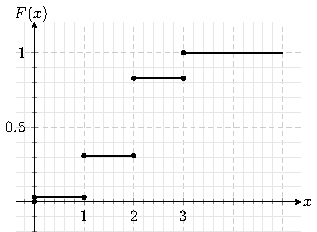
\includegraphics[width=0.5\linewidth]{mai_fig045.pdf}
      \caption{Distribuční funkce k příkladu \ref{mai:exam064}. \cite[s.~233]{Musilova2009MA1}}
      \label{mai:fig045}
    \end{figure}
    Zadáním distribuční funkce je naopak jednoznačně určeno rozdělení veličiny \(X\). Pro jednotlivé
    pravděpodobnosti totiž platí
    \begin{equation*}
      p_j = F(x_j) - F(x_{j-1})\qquad\text{pro}\qquad 2\leq j \leq k, \qquad p_1 = F(x_1).
    \end{equation*}
    
    Hledejme nyní hodnotu \(\overline{x}_P\) definovanou tak, že pravděpodobnost, že při náhodném 
    opakování pokusu nabude veličina \(X\) kterékoli z přípustných hodnot \(x_j \leq 
    \overline{x}_p\), je rovna \(P\). Znamená to, že pro \(x = \overline{x}_P\) má distribuční 
    funkce nabýt předepsané hodnoty \(P\). Abychom \(\overline{x}_P\), takzvaný 
    \(P\)\textbf{-kvantil}, určili, řešíme rovnici
    \begin{equation}\label{mai:eq064}
      \sum_{j=1}^{s}p_j = P
    \end{equation}
    vzhledem k neznámému počtu sčítanců \(s\). V případě veličiny s diskrétním rozdělením se ovšem
    může stát, že pro nevhodně zvolenou hodnotu \(P\) nebude mít rovnice řešení. To proto, že 
    veličina \(X\) může nabývat jen hodnot, které lze očíslovat přirozenými čísly, takže při každé 
    změně horní meze sumy \(s\) o jedničku se suma mění skokem. Vidíme to jak v předcházející 
    tabulce, tak v grafu na obrázku \ref{mai:fig045}. Pro \(P = \num{0.5}\) se \(P\)-kvantil 
    \(\overline{x}_p\), pokud je vůbec definován, nazývá \textbf{medián}. Značí se pouze 
    \(\overline{x}\).

    %--Ještě střelba------------------------------------------------
    % !TeX spellcheck = cs_CZ
\begin{mdframed}[style=mdexam]
  \begin{example}\label{mai:exam067}
    \textbf{Ještě střelba}\newline
    Problém s definici \(P\)-kvantilu u veličiny s diskrétním rozdělením snadno vidíme na příkladu
    střelby (příklad \ref{mai:exam064}). Pro \(s\) postupně 1, 2, 3, 4 nabývá součet na levé straně
    rovnice (\ref{mai:eq064}) hodnot
    
    \begin{equation*}
      p_1 = \num{0.003},\; p_1 + p_2 = \num{0.31},\; p_1 + p_2 + p_3 = \num{0.83}, 
    \end{equation*}
    \begin{equation*}
      p_1 + p_2 + p_3 + p_4 = 1.
    \end{equation*}
    Pojem \(P\)-kvantil je tedy definován jen pro \(P = 0\), \(P = \num{0.03}\), \(P = \num{0.31}\),
    \(P = \num{0.83}\) a \(P = 1\). (Pro \(P = 0\) a \(P = 1\) nemá žádný praktický význam.)
    Nenabývá-li \(P\) žádné z přípustných hodnot, tj. některé hodnoty z množiny \(\{\num{0.03},
    \num{0.31}, \num{0.83}, 1\}\), nemá rovnice pro s řešení a \(P\)-kvantil není vůbec definován.
    Je-li hodnotou \(P\) některý prvek této množiny, dostaneme z rovnice (\ref{mai:eq064}) sice
    jediné řešení \(s\), avšak která hodnota bude \(P\)-kvantilem? Z grafu je vidět, že pro každou
    přípustnou hodnotu \(P\) vyhovuje podmínce celý interval proměnné \(x\). Konkrétní výsledky
    shrnuje následující tabulka:
    
    {\centering
      \begin{tabular}{c|@{\hspace{3pt}}c@{\hspace{3pt}}c@{\hspace{3pt}}c@{\hspace{3pt}}c@{\hspace{3pt}}c}
        \(P\) & \num{0} & \num{0.03} & \num{0.31} & \num{0.83} & \num{1} \\ \hline
        \(F(x) = P\) & \((-\infty,\num{0})\) & \(\left[0, 1\right)\) &
        \(\left[1, 2\right)\) & \(\left[2, 3\right)\) & \(\left[3, \infty\right)\)
      \end{tabular}
    \par}
    
    Význam pojmu \(P\)-kvantil je tedy pro náhodnou veličinu s diskrétním rozdělením poněkud sporný.
    Uplatní se však velmi dobře u veličin s rozdělením spojitým, jak uvidíme později. Než však
    opustíme příklad se střelbou definitivně, spočtěme si ještě střední hodnotu a rozptyl veličiny
    \(X\), kterou jsme definovali jako počet dosažených bodů při jednom výstřelu:
    \begin{align*}
      \langle x \rangle 
          &= \sum_{j=1}^{4}x_jp_j                                                                \\
          &= 0\cdot\num{0.03} + 1\cdot\num{0.28}+ 2\cdot\num{0.52} + 3\cdot\num{0.17} = \num{1.83}, 
    \end{align*}
    \begin{align*}
      D(X)  &= \sum_{j=1}^{4}\left(x_j - \langle x \rangle \right)^2p_j                          \\
            &= (0-\num{1.83})^2\cdot\num{0.03}+(1-\num{1.83})^2\cdot\num{0.28}                   \\
            &+ (2-\num{1.83})^2\cdot\num{0.52}+(3-\num{1.83})^2\cdot\num{0.17}                   \\
                &\simeq\num{0.541},                                                              \\
      \sigma(x) &\simeq\num{0.736}.
    \end{align*}

    V příkladu \ref{mai:exam064} jsme odhadovali, kolika bodů dosáhne střelec při pěti výstřelech.
    Tato hodnota nám vyšla \(\num{5}\cdot\num{1.83} = \num{9.15} = 9\). Nyní vidíme je jí souvislost
    se střední hodnotou náhodné veličiny \(X\). Pokud totiž definujeme veličinu \(Y\) jako počet
    bodů dosažených při pěti výstřelech, je \(Y = 5X\) a \(\langle y \rangle = 5\langle x \rangle\).
    Uvažujme nyní o významu směrodatné odchylky. Zřejmě \(\sigma(y) = 5\sigma(x) = \num{3.68}\).
    Směrodatná odchylka \(\sigma(y)\) určuje interval \((\langle y \rangle - \sigma(y), \langle y
    \rangle + \sigma(y)) = (\num{5.32}, \num{12.68})\). Možnosti bodového zisku ležící v tomto
    intervalu jsou \num{6} až \num{12} bodů včetně. Pokud bychom doplnili tabulku z příkladu
    \ref{mai:exam064} ještě o rozklady a jejich pravděpodobnosti pro bodový součet při pěti
    výstřelech \(j = \num{6}\) a \(j = \num{12}\), dostaneme \(p(A_6) = \num{0.0400}\), \(p(A_{12})
    = \num{0.0550}\). Pravděpodobnost, že výsledek střelce leží při pěti výstřelech v intervalu
    \((\langle y \rangle - \sigma(y), \langle y \rangle + \sigma(y)) = (\num{5.32}, \num{12.68})\),
    je tedy
    \begin{align*}
      \sum_{j=6}^{12}p(A_j) &= p(A_6) + \sum_{j=7}^{11}p(A_j) + p(A_{12})                \\
                            &= \num{0.0400} + \num{0.873} + \num{0.0550} \simeq \num{0.97}.
    \end{align*}
    Při výpočtu jsme využili výsledku z příkladu \ref{mai:exam064}, kde jsme počítali
    pravděpodobnost, že střelec dosáhne bodového výsledku v rozmezí \num{7} až \num{11} bodů.
    Směrodatná odchylka \(\sigma(y)\) veličiny \(Y\) určuje tedy v tomto případě interval okolo
    střední hodnoty \(\langle y \rangle\), v němž leží střelcův bodový zisk s velmi vysokou
    pravděpodobností \SI{97}{\percent}. Tento výsledek lze velmi názorně interpretovat také takto:
    Vystřelí-li střelec pětkrát na terč, bude téměř s jistotou jeho bodový zisk ležet v intervalu
    určeném směrodatnou odchylkou, tj. bude ležet mezi šesti a dvanácti body. Není vyloučeno, že
    bodový zisk bude třeba pět bodů, nebo i nula, nebo naopak dokonce maximálních možných patnáct
    bodů. Všechny ty to možnosti dohromady jsou však vysoce nepravděpodobné, připadá na ně
    pravděpodobnost pouhé \SI{3}{\percent}!. Anebo ještě trochu jinak: Kdyby střelec při tréninku
    uskutečnil třeba sto sérií po pěti výstřelech, pak by skoro jistě bylo sedmadevadesát z nich v
    rozmezí bodového zisku \num{6} až \num{12} bodů a tři mimo. Toto konstatování ovšem opět
    nevylučuje možnost, že v rozmezí \num{6} až \num{12} bodů bude ležet jiný počet sérií než
    \num{97}. Může dokonce v principu dojít k tomu, že do této kategorie padnou série všechny nebo
    žádná. Takový výsledek je však opět vysoce nepravděpodobný.
    
    Není vyloučeno, že i po prostudování tohoto příkladu bude někdo stále nespokojen s tím, že je
    naše vyjadřování „málo přesné“. Vzhledem k pravděpodobnostnímu charakteru posuzovaných jevů
    však, bohužel, přesnější být nemůže.
  \end{example}
\end{mdframed}
    %---------------------------------------------------------------
    
    Příklad \ref{mai:exam067} názorně vypovídá o významu směrodatné odchylky. Viděli jsme, že 
    intervalu o šířce \(2\sigma(y)\) s hodnotou \(\langle y \rangle\) uprostřed odpovídá vysoká 
    pravděpodobnost, že v něm bude ležet bodový zisk střelce při každé pětici výstřelů. Čím bude 
    tento interval užší, tím v průměru blíže budou jednotlivé hodnoty bodového zisku ležet v 
    blízkosti střední hodnoty. Mohli bychom říci, že střelec, jehož výsledky vykazují malou 
    směrodatnou odchylku resp. malý rozptyl, míří přesněji. Směrodatná odchylka je tedy v jistém 
    smyslu jedním z parametrů charakterizujících kvalitu střelby - střelba s malou hodnotou  
    \(\sigma(y)\) je přesnější než střelba s velkou hodnotou \(\sigma(y)\). Druhým parametrem 
    kvality střelby, který je pro její hodnocení z hlediska možnosti vyhrávat soutěže jistě 
    podstatně důležitější, je samozřejmě samotná střední hodnota bodového zisku. Čím je větší, tím 
    je střelcovo pořadí při závodech lepší. Pro interpretaci směrodatné odchylky to ovšem není 
    podstatné. Kdybychom porovnávali dva střelce, jejichž střední bodový zisk při
    pěti výstřelech je třeba \num{12} bodů a \num{3} body, avšak směrodatná odchylka je u obou 
    stejná, musíme konstatovat, že oba jsou stejně přesní. Jeden z nich však systematicky dělá 
    nějakou chybu a přesně střílí do nesprávného místa. Význam pojmu přesnost z hlediska hodnocení 
    náhodných veličin je tedy oproti jeho běžnému chápání poněkud posunut.
    
    Všimněme si ještě jedné důležité obecné věci: Tvar vzorce pro výpočet rozptylu resp. směrodatné 
    odchylky je stejný pro všechny typy rozdělení. Konkrétní pravděpodobnost, že hodnota
    veličiny padne do intervalu určeného směrodatnou odchylkou, tj. do intervalu \((\langle y 
    \rangle - \sigma(y), \langle y \rangle + \sigma(y))\), však pochopitelně na konkrétním 
    rozdělení závisí.

    %--Poissonovo rozdělení-----------------------------------------
    % !TeX spellcheck = cs_CZ
\wikitextrule
\begin{example}\label{mai:exam068}
  \textbf{Poissonovo rozdělení}\newline\small
  Limitním případem Bernoulliova (binomického) rozdělení pro velké hodnoty \(n\), tj. \(n 
  \rightarrow \infty\), a pro \(j \ll n\) je \textbf{rozdělení Poissonovo}. Odvodíme je. Pro velká 
  \(n\) a \(j \ll n\) platí přibližný vzorec
  \begin{equation*}
    n! \simeq n^j(n-j)!,
  \end{equation*}
  a tedy
  \begin{equation*}
    P_j \simeq \lim\limits_{n\rightarrow\infty}\dfrac{n^j}{j!}p^j(1-p)^{n - j}
        \simeq \lim\limits_{n\rightarrow\infty}\dfrac{(np)^j}{j!}\left(1-\dfrac{np}{n}\right)^{n}.
  \end{equation*}
  Při vzpomínce na kapitolu o počítání i limitami a na \textbf{l’Hospitalovo pravidlo} snadno 
  provedeme následující výpočet. O testujte své předchozí znalosti a jednotlivé kroky výpočtu 
  proveďte:
  \begin{equation*}
    \lim\limits_{n\rightarrow\infty}\left(1 - \dfrac{A}{n}\right)^n = 
    \lim\limits_{x\rightarrow0}\left(1 - Ax\right)^\dfrac{1}{x} =
    \exp\left(\lim\limits_{x\rightarrow0}\dfrac{\ln(1 - Ax)}{x}\right) = e^{-A}.
  \end{equation*}
  V našem případě je \(A = np = \langle x \rangle\) (střední hodnota veličiny \(X\) při 
  Bernoulliově rozdělení), takže
  \begin{equation}\label{mai:eq065}
    p_j = \langle x \rangle^j\dfrac{e^{-\langle x \rangle}}{j!}.
  \end{equation}
  Možnost použití Bernoulliova rozdělení si již představit dokážeme. Přinejmenším jsou hody mincemi 
  a kostkami pěkné hříčky. K čemu však je dobré rozdělení Poissonovo? Ja k může vypadat praktická 
  situace, kdy provádíme obrovské množství opakování pokusu a zajímá nás pravděpodobnost pouze 
  malého počtu zdarů? Typickým příkladem takové situace je registrace částic vznikajících při 
  radioaktivním rozpadu. Taková měření jsou potřebná nejen ve fyzikálním výzkumu, ale i v 
  aplikovaných oborech, například v lékařství. Počet \(n\) radioaktivních rozpadů za jednotku času, 
  například za sekundu, je u běžných zdrojů obrovský, zatímco počet těch z nich, které jsou 
  zachycovány detektorem, může být při určitých experimentech malý. Částice se registrují
  pomocí Geigerova-Mullerova počítače, kterým je ionizační komora pracující ve vhodném režimu. 
  Pokud je počet částic \(j\) dopadajících za jednu sekundu do detektoru velmi malý, vyvolá každá z 
  nich měřitelný a dokonce slyšitelný pulz (v obvodu to „praská“). Po registraci částice potřebuje 
  detektor jistou \textbf{mrtvou dobu}, aby se vrátil do výchozího stavu, v němž je schopen 
  registrovat další částici. Tato doba se pohybuje kolem \SI{e-4}{s}. Aby byly jednotlivé pulzy 
  dobře odlišeny, je však třeba, aby do detektoru dopadlo za jednu sekundu mnohem a mnohem méně 
  částic, než jak by odpovídalo převrácené hodnotě mrtvé doby. Zejména pokud bychom chtěli pulzy 
  počítat sluchem, nemělo by jich být více než zhruba jeden až dva každou sekundu. Uvažujme o 
  radioaktivním rozpadu jader cesia \ce{Cs^137}. Jedná se o takzvaný \textbf{beta-rozpad}, který 
  probíhá následovně:
  \begin{itemize}
    \item \ce{Cs^137} \(\longrightarrow\) \ce{Ba^137} + elektron + neutrino, asi \SI{8}{\percent} 
          všech rozpadů
    \item \ce{Cs^137} \(\longrightarrow\) \ce{Ba^137}* + elektron + neutrino, asi \SI{92}{\percent} 
          všech rozpadů
  \end{itemize}
  Excitované baryum \ce{Ba^137}* (jádro má vyšší energii než atom \ce{Ba^137} v základním stavu 
  asi o \SI{0.66}{\mega\electronvolt}  - odpovídá energii \SI{1.1e-13}{\joule}) se pak dále rozpadá 
  podle vzorce
  \begin{itemize}
    \item \ce{Ba137}* \(\longrightarrow\) \ce{Ba137} + částice gama.
  \end{itemize}

  Ze všech částic, které při reakci vznikají, se v Geigerově-Můllerově detektoru registrují 
  elektrony a částice gama, nelze je však od sebe odlišit. Uvažujme o cesiovém zdroji s běžnou 
  hodnotou aktivity, například \SI{10}{\pico\coulomb} (mikrocurie). Jednotka aktivity 
  radioaktivních preparátů \num{1} curie představuje situaci, kdy se za jednu sekundu rozpadá 
  \num{3.7e10} jader. Počet rozpadů, které v průměru nastanou třeba za deset sekund v našem vzorku, 
  je \(n = \num{3700000}\). V Bernoulliově pokusu to odpovídá počtu jeho opakování \(n\). Ja k jsme 
  již řekli, je to obrovský počet. Nastavíme-li experiment tak, abychom registrovali každou sekundu 
  zhruba jednu částici (uslyšíme jeden „prásk“ ), bude počet zdarů \(j\) v Bernoulliově pokusu 
  velmi malý ve srovnání s \(n\). Jsou tedy splněny podmínky pro použití Poissonova rozdělení. 
  Zvolíme například desetisekundový interval měření a počítáme pulzy. Počet registrovaných pulzů 
  \(j\) v tomto intervalu je roven počtu zdarů. Takové měření provedeme třeba dvěstěkrát.
  Označme počet intervalů, v nichž jsme naměřili právě \(j\) pulzů, jako \(\nu(j)\). Celkem je v 
  \(\nu(1) + \cdots + \nu(j_{max}) = \num{200}\). Získáme tak tabulku nebo graf, z nichž pak lze 
  usuzovat na parametry Poissonova rozdělení:
  \begin{table}[ht!]
    \centering
    \resizebox{0.8\textwidth}{!}{%
    \begin{tabular}{c|crrrrrrrrrrrrrrrrr}
      \(j\)      & 0 & 1 & 2 & 3 & 4 & 5 & 6 & 7 & 8 & 9 & 10 & 11& 12& 13 & 14 & 15 & 16 & 17   \\
      \hline
      \(\nu(j)\) & 0 & 4 & 10 & 19 & 28 & 33 & 34 & 26 & 19 & 10 & 6 & 3 & 2 & 2 & 2 & 0 & 1 & 1 \\
    \end{tabular}}
    % \caption{ }
  \end{table}
  Budeme-li předpokládat, že větší počet pulzů v desetisekundovém intervalu je již velmi málo 
  pravděpodobný, můžeme četnosti \(\nu(j)\) považovat za úměrné pravděpodobnostem \(p_j\) 
  Poissonova rozdělení. Všimněme si formule pro Poissonovo rozdělení podrobněji. Je vidět, že platí
  \begin{equation*}
    \dfrac{\nu(j + 1)}{\nu(j)} = \dfrac{p_{j+1}}{p{j}} = \dfrac{\langle x \rangle}{j + 1},
    \qquad p_0 = e^{-\langle x \rangle}.
  \end{equation*}
  Pro hodnotu \(j\), pro kterou jsou si četnosti \(\nu(j)\) a \(\nu(j + 1)\) „nejblíže“, je 
  \(\langle x \rangle \simeq j + 1\). Z tabulky vidíme, že v případě našeho experimentu je 
  \(\langle x \rangle = 6\). Hodnota \(p_0 = e^{-6} \simeq \num{0.002}\) je tedy tak malá, že se 
  ani nedivíme, že jsme mezi dvěma stovkami měření nezaznamenali ani jeden případ, kdy v 
  desetisekundovém intervalu nebyla zaregistrována žádná částice.
  
  Můžeme ještě určit podíly sousedních hodnot \(\nu(j + 1)\) a \(\nu(j)\) a zjistit, zda výsledky 
  našeho experimentu odpovídají vlastnostem Poissonova rozdělení:
  \begin{table}[ht!]
    \centering
    \resizebox{0.7\textwidth}{!}{%
    \begin{tabular}{c|crrrrrrrr}
      \(j\)               & 0 & 1 & 2  & 3  & 4  & 5  & 6  & 7 & 8    \\ \hline
      \(\nu(j+1)/\nu(j)\) & - & \num{2.50} & \num{1.90} & \num{1.47} & \num{1.18} 
                          & \num{1.03} & \num{0.76} & \num{0.73} & \num{0.53}   \\
      \(\langle x \rangle / j + 1\) & \num{6.00} & \num{3.00} & \num{2.00} & \num{1.50} & \num{1.20}
                          & \num{1.00} & \num{0.86} & \num{0.75} & \num{0.67}
    \end{tabular}}
    % \caption{ }
  \end{table}
  \begin{table}[ht!]
    \centering
    \resizebox{0.7\textwidth}{!}{%
    \begin{tabular}{c|crrrrrrrr}
      \(j\)               & 9 & 10 & 11  & 12  & 13  & 14  & 15  & 16 & 17    \\ \hline
      \(\nu(j+1)/\nu(j)\) & \num{0.60} & \num{0.50} & \num{0.67} & - & - & - & - & - & -   \\
      \(\langle x \rangle / j + 1\) & \num{0.60} & \num{0.55} & \num{0.50} & \num{0.46}
                          & \num{0.43} & \num{0.40} & \num{0.38} & \num{0.35} & \num{0.33}
    \end{tabular}}
    % \caption{ }
  \end{table}
  Vidíme, že hodnoty podílů sousedních četností celkem dobře odpovídají vlastnostem Poissonova 
  rozdělení pro \(0 \leq j \leq 12\). Pro \(j > 12\) jsou již četnosti \(\nu(j)\) tak malé, že 
  vytvářet jejich podíly nemá smysl. Tato skutečnost je v tabulce vyznačena pomlčkou.
  
  Poissonovým rozdělením se řídí také například četnost červených krvinek, které se v daném časovém 
  intervalu objeví ve vymezené části zorného pole mikroskopu, četnost zmetků v dodávce zboží, 
  četnost překlepů písařky, apod.  
\normalsize
\end{example}
    %---------------------------------------------------------------
    
    \subsection{Kolik rychlostí má molekula plynu - spojité rozdělení}
      Již nadpis napovídá, že veličina se spojitým rozdělením může zřejmě nabývat „spojitě 
      rozložených“ hodnot, tj. přípustným i hodnotami budou například právě všechna čísla \(x\) z 
      jistého intervalu, \(x\in[a, b]\). Jaká však bude pravděpodobnost \(p(x)\), že veličina \(X\) 
      nabývá právě hodnoty \(x\in[a, b]\)? Jestliže víme, že „součet“ všech \(p(x)\) musí být roven 
      jedné, vzniká problém.
      
      Hodnot \(x\) je totiž nekonečně (dokonce nespočetně) mnoho! Je jich tolik, jako je čísel na 
      celé reálné ose. A kdyby byla pravděpodobnost \(p(x)\) jakkoli malinkatá, nikdy nebude součet 
      všech \(p(x)\) konečný. Pravděpodobnost nabývání hodnoty \(x\) tedy musí být nulová. Vzniklou 
      překážku odstraníme snadno. Rozdělení náhodné veličiny \(X\) bude nutno charakterizovat 
      nikoli pravděpodobností, ale \textbf{hustotou pravděpodobnosti}. Je to obdobná situace jako 
      třeba při popisu rozložení hmotnosti nějakého tělesa, předpokládáme-li, že je ta to hmotnost 
      rozložena v objemu tělesa spojitě. Také nemá příliš smysl se ptát, jaká je hmotnost jednoho 
      bodu tohoto tělesa. I zde by byla odpověď, že nulová. Spíše si vždy klademe otázku, jaká je 
      hmotnost \(\Delta m(\vec{r})\) jistého malého objemu \(\Delta V\), například malého kvádříku, 
      umístěného třeba jedním z vrcholů v bodě o poloze \(\vec{r}\). Hustota \(\varrho(\vec{r})\) 
      tělesa v bodě \(\vec{r}\) je pak limitou podílu \(\Delta m(\vec{r})/\Delta V\) pro \(\Delta V 
      \longrightarrow 0\). Obdobně je tomu i s rozdělením spojité náhodné veličiny \(X\). 
      Zvolíme-li pro jistou hodnotu \(x\) interval \([a, x + \Delta x]\), má smysl otázka, jaké je 
      pravděpodobnost \(\Delta p(x)\), že veličina nabývá hodnoty (kterékoli) právě z tohoto 
      intervalu.

      \adjustbox{minipage=[c]{\textwidth}}{%
        Limitu
        \begin{equation}\label{mai:eq066}
          w(x) = \lim\limits_{\Delta\longrightarrow0}\dfrac{\Delta p(x)}{\Delta x}
        \end{equation}
        nazýváme \textbf{hustotou pravděpodobnosti} veličiny \(X\) v bodě \(x\) (pro \(x = a\), 
        resp. \(x = b\) se jedná o limitu zprava, resp. zleva).
      }
      
      Přímo tato funkce pak představuje ono spojité rozdělení náhodné veličiny \(X\). Určuje totiž
      hustotu pravděpodobnosti \(w\) pro hodnotu \(x\) náhodné veličiny \(X\), obdobně jako \(p_j\) 
      v případě diskrétního rozdělení určuje pravděpodobnost hodnoty \(x_j\). Předpokládejme, že je 
      funkce \(w(x)\) na intervalu \([a, b]\) spojitá.
  
      \adjustbox{minipage=[c]{\textwidth}}{%
        Pro \(x \in [a, b]\) definuje integrál jako funkce horní meze
        \begin{equation}\label{mai:eq067}
          F(x) = \int_a^xw(u)\dd{u}
        \end{equation}
        \textbf{distribuční funkci}.
      }
      Jeho hodnota pro dané \(x\) udává pravděpodobnost, že hodnota veličiny \(X\) padne do 
      intervalu \([a, x]\), opět v plné analogii s případem diskrétního rozdělení. Na \((a, b)\) je 
      tedy hustota pravděpodobnosti \(w(x)\) derivací distribuční funkce. Je zřejmé, že \(F(b) = 
      1\). Integrál z hustoty pravděpodobnosti v mezích \([a, b]\) udává totiž pravděpodobnost, že 
      hodnota veličiny \(X\) padne do intervalu přípustných hodnot, tedy pravděpodobnost jistého 
      jevu. V případě diskrétního rozdělení jsme však distribuční funkci definovali nejen pro 
      přípustné hodnoty náhodné veličiny, ale pro všechna x \in (-\infty, +\infty). Tento postup 
      budeme respektovat i nyní a definujeme
      \begin{equation*}
        F(x) = 0\text{ pro }x \in (-\infty,a)\text{ a }F(x) = 1\text{ pro }x \in (b , +\infty).
      \end{equation*}
      \adjustbox{minipage=[c]{\textwidth}}{%
        \begin{equation}\label{mai:eq068}
          \langle x \rangle = \int_a^bxw(x)\dd{x}, \qquad 
                       D(X) = \int_{a}^{b}(x - \langle x \rangle)^2w(x)\dd{x}.
        \end{equation}
      }
      \textbf{Relativní směrodatná odchylka} je opět podílem \(\sqrt{D(X)}/\langle x \rangle\), 
      nejpravděpodobnější hodnota neboli \textbf{modus} \(x_m\) je taková hodnota veličiny \(X\) , 
      pro kterou je hustota pravděpodobnosti maximální
      
      Daleko lépe než u veličin s diskrétním rozdělením vypadá možnost definovat \(P\)-kvantil 
      \(\tilde{x}_p\) a \textbf{medián} \(\tilde{x}\). Jsou jednoduše řešením rovnic
      \begin{equation*}
        F(\tilde{x}_P) = P, \qquad F(\tilde{x}) = \dfrac{1}{2}
      \end{equation*}
      (Mohli bychom mediánu třeba i říkat „půlkvantil“. To ale není zvykem.) \(P\)-kvantil je 
      definován pro jakoukoli hodnotu \(P\) zadanou v intervalu \((0, 1)\). Skutečně, hustota 
      pravděpodobnosti je nezápornou funkcí na intervalu \([a, b]\) (podle předpokladu i spojitou), 
      takže distribuční funkce je na \([a, b]\) \emph{spojitá} a \emph{rostoucí} a nabývá hodnot 
      \(0 = F(a) \leq F(x) \leq F(b) = 1\). Podle jedné z vět o spojitých funkcích (odstavec 
      2.1.7*) nabývá funkce spojitá na uzavřeném intervalu všech hodnot mezi svým minimem a 
      maximem. V intervalu \([a, b]\) tedy existuje alespoň jedna hodnota \(\tilde{x}_P\) , pro 
      kterou je \(F(\tilde{x}_P) = P\). Ze skutečnosti, že je \(F(x)\) navíc rostoucí, vyplývá, že 
      i \(\tilde{x}_P\) existuje jednoznačně.
  
      Tyto závěry zůstanou v platnosti, i kdyby veličina \(X\) nabývala svých hodnot v intervalu
      typu \(\left[0, \infty\right), \left(—\infty, b\right]\) nebo \((—\infty, \infty)\). Vzhledem 
      k požadavku
      \begin{equation*}
        \int_{a}^{b}w(x)\dd{x} = 1,
      \end{equation*}
      kde kterákoli z mezí \(a\), resp. \(b\) může být i nevlastní, je zřejmé, že funkce \(w(x)\) 
      musí být na svém definičním oboru \(D_f\) omezená. Navíc je na něm spojitá. Vybereme-li tedy 
      jakýkoli uzavřený podinterval oboru \(D_f\), můžeme předchozí argumentaci týkající se 
      \(P\)-kvantilu bez problémů použít.

      %--Normální rozdělení-------------------------------------------
      % !TeX spellcheck = cs_CZ
\begin{mdframed}[style=mdexam]
\begin{example}\label{mai:exam069} \textbf{Normální rozdělení}\\
  Veličinou s normálním rozdělením rozumíme takovou náhodnou veličinu \(X\), jejíž hustota 
  pravděpodobnosti má tvar
  \begin{mdframed}[style=highlight]
    \begin{equation}\label{mai:eq069}
      w(x) = \dfrac{1}{\sigma\sqrt{2\pi}}\exp\left[-\dfrac{(x-\mu)^2}{2\sigma^2}\right],
             \qquad x\in(-\infty, \infty).
    \end{equation}
  \end{mdframed}
  Grafem této funkce je \textbf{Gaussova křivka}. Distribuční funkce má tvar
  \begin{mdframed}[style=highlight]
    \begin{equation}\label{mai:eq70}
      F(x) = \int_{-\infty}^{x}\dfrac{1}{\sigma\sqrt{2\pi}}
               \exp\left[-\dfrac{(t-\mu)^2}{2\sigma^2}\right]\dd{t}.
    \end{equation}
  \end{mdframed}
  udává pravděpodobnost, že hodnota náhodné proměnné je menší než zadaná hodnota (nerovnost může 
  být i neostrá). Přitom \(F(\infty) = 1\) (pravděpodobnost jistého jevu). Skutečně, platí
  \begin{equation*}
    \begin{multlined}
      \int_{-\infty}^{\infty}\dfrac{1}{\sigma\sqrt{2\pi}}
      \exp\left[-\dfrac{(t-\mu)^2}{2\sigma^2}\right]\dd{t}   \\
      \shoveleft[1cm]= \dfrac{\sigma\sqrt{2}}{\sigma\sqrt{2\pi}}
              \int_{-\infty}^{\infty}\exp\left(-u^2\right)\dd{u} =1.
    \end{multlined}
  \end{equation*}
  Takzvaný Laplaceův integrál \(\int_{-\infty}^{\infty}\exp(-u^2)\dd{u} = \sqrt{\pi}\) 
  sice můžeme najít v tabulkách a v dalším dílu jej i odvodíme, v tu to chvíli se však budeme řídit 
  výrokem lorda Kelvina: „Matematik je ten, komu je toto zřejmé jako je zřejmé vám, že dvakrát dvě 
  jsou čtyři.“ Příklady normálního rozdělení pro různé hodnoty \(\sigma,\,\mu\) a odpovídající 
  distribuční funkce vidíme na obrázku \ref{mai:fig046a} a \ref{mai:fig046b}.

  {\centering
    \captionsetup{type=figure}
     \subcaptionbox{\label{mai:fig046a}}{\luafigure[1]{mai_fig046a.pdf}}              \\
     \subcaptionbox{\label{mai:fig046b}}{\luafigure[1]{mai_fig046b.pdf}}
     \captionof{figure}{Hustota pravděpodobnosti normálních rozdělení a jejich distribuční funkce 
              s různými charakteristikami \(\sigma\) a \(\mu\). Červenou čárou je vyznačeno 
              normované normální rozdělení. \cite[s.~240]{Musilova2009MA1}
    \label{mai:fig046}}
  \par}
  \vspace*{10px} Určíme střední hodnotu a rozptyl veličin s tímto rozdělením:
  \begin{align*}
    \langle x \rangle 
      &= \int_{-\infty}^{x}\dfrac{1}{\sigma\sqrt{2\pi}}x\cdot
         \exp\left[-\dfrac{(x-\mu)^2}{2\sigma^2}\right]\dd{x}                                     \\
      &= \dfrac{\sigma\sqrt{2}}{\sigma\sqrt{2\pi}}
         \int_{-\infty}^{\infty}\left(\mu+t\sigma\sqrt{2}\right)\cdot\exp\left(-t^2\right)\dd{t}  \\
      &= \dfrac{\mu}{\sqrt{\pi}}\int_{-\infty}^{\infty}\exp\left(-t^2\right)\dd{t}                \\
      &+ \dfrac{1}{\sqrt{\pi}}\int_{-\infty}^{\infty}t\sigma\sqrt{2}\cdot\exp\left(-t^2\right)\dd{t}
       =\mu.
  \end{align*}
  Druhý z integrálů je totiž roven nule, neboť integrand je lichá funkce.
  \begin{align*}
    D(X)  &= \dfrac{1}{\sigma\sqrt{2\pi}}\int_{-\infty}^{\infty}\left(x - \mu\right)^2 
             \exp\left[-\dfrac{(x-\mu)^2}{2\sigma^2}\right]\dd{x}                                \\
          &= \dfrac{2\sqrt{2}\sigma^3}{\sigma\sqrt{2\pi}}
             \int_{-\infty}^{\infty}t^2\exp\left(-t^2\right)\dd{t}
           = \sigma^2.
  \end{align*}
  Integrál \(\int_{-\infty}^{\infty}t^2\exp\left(-t^2\right)\dd{t} = \frac{\sqrt{\pi}}{2}\) lze buď 
  opět najít v tabulkách, nebo jej metodou per partes převést na výpočet Laplaceova integrálu:
  \begin{align*}
    I &= \int_{-\infty}^{\infty}t\cdot t\exp\left(-t^2\right)\dd{t}         \\
      &= \left[-\dfrac{t}{2}\exp\left(-t^2\right)\right]_{-\infty}^{\infty}
       + \dfrac{1}{2}\int_{-\infty}^{\infty}\exp\left(-t^2\right)\dd{t}.
  \end{align*}
  
  Distribuční funkce normálního rozdělení, zvaná \(errorfunkce\), je běžnou součástí různých 
  počítačových programů, takže poměrně snadno zjistíme pravděpodobnostní obsah intervalu určeného 
  směrodatnou odchylkou \(\sigma(x) = \sqrt{d(X)} = \sigma\). Pravděpodobnost, že hodnota náhodné 
  veličiny \(X\) s normálním rozdělením leží v intervalu \((\mu - \sigma, \mu + \sigma)\), je 
  zhruba \SI{68.3}{\percent}. V souvislosti s normálním rozdělením se často užívají další 
  dva druhy odchylek. \textbf{Pravděpodobná chyba} \(\theta\) určuje interval \((\mu - \theta, \mu 
  + \theta)\), v  němž leží hodnota veličiny \(X\) s pravděpodobností \SI{50}{\percent}. 
  \textbf{Krajní chyba} \(\kappa\) určuje interval \((\mu - \kappa, \mu + \kappa)\), v němž leží 
  hodnota veličiny \(X\) s pravděpodobností \SI{99.7}{\percent}. Z tabelovaných hodnot 
  \(errorfunkce\) zjistíme, že platí
  \begin{equation}\label{mai:eq71}
   \theta \simeq \dfrac{2}{3}\sigma, \qquad \kappa = 3\sigma
  \end{equation}
  Poznamenejme, že normálním rozdělením \(w(x)\) (\ref{mai:eq069}) lze přibližně nahradit 
  Bernoulliovo rozdělení
  \begin{align*}
    w_{Ber}(x)        &= \binom{n}{x}p^x(1 - p)^{n-x},  \\
    \langle x \rangle &= np, \;  D(x) = np(1-p)
  \end{align*}
  pro velké hodnoty \(n\) a také Poissonovo rozdělení
  \begin{equation*}
    w_{Pois}(x) = e^{-\langle x \rangle}\dfrac{\langle x \rangle^x}{x!}, \qquad 
    D(x) = \langle x \rangle
  \end{equation*}
  s velkou střední hodnotou \(\langle x \rangle\)
\end{example}
\end{mdframed}
      %---------------------------------------------------------------
  
      %--Kolik rychlostí má molekula plynu----------------------------
      % !TeX spellcheck = cs_CZ
\wikitextrule
\begin{example}\label{mai:exam070}
  \textbf{Kolik rychlostí má molekula plynu}\newline\small
  Tato otázka se zdá na první pohled zcela nesmyslná. Každý student fyziky ví, že molekuly plynu 
  lze popisovat jako klasické částice, jejichž mechanický stav je jednoznačně určen polohovým 
  vektorem a vektorem rychlosti. Molekula má tedy vždy určitou hodnotu rychlosti. Představte si ale 
  takový plyn ve skutečnosti. Jeden mol jeho látkového množství (např. pro kyslík to představuje 
  hmotnost \num{32} gramů) obsahuje asi \num{6.623e23} molekul! Kdybychom chtěli plyn popisovat 
  jako soustavu klasických částic v mechanice, museli bychom v daném okamžiku znát polohu a 
  rychlost každé molekuly z tohoto obrovského počtu. A to je principiálně nemožné, protože do 
  chování takové soustavy zasahuje velmi podstatným způsobem „náhoda“. Nemůžeme určit, ve kterém
  bodě prostoru právě daná molekula je a jak rychle se pohybuje. Dokážeme pouze určit, s jakou 
  pravděpodobností se nachází v elementárním objemu \(\Delta V = \Delta x \Delta y \Delta z\) v 
  okolí daného bodu o polohovém vektoru \(\vec{r}\) a s jakou pravděpodobností \(\Delta P\) leží 
  koncový bod vektoru její rychlosti v elementárním objemu \(\Delta\Omega = \Delta v_x \Delta v_y 
  \Delta v_z\) „rychlostního“ prostoru v okolí zadané rychlosti \(\vec{v}\). Uvažujme o 
  nejjednodušším modelu plynového tělesa, takzvaném ideálním plynu, jehož molekuly jsou stejné a 
  navzájem neinteragují s výjimkou kratičkých náhodných srážek. Molekuly takového plynu jsou z 
  hlediska pravděpodobnostního popisu navzájem ekvivalentní. Pravděpodobnost \(\Delta P\) bude pro 
  všechny stejná a pro velmi malé elementární objemy bude dána vztahem
  \begin{equation*}
    \Delta P(\vec{r},\vec{v}) = \varrho(\vec{r},\vec{v})\Delta V \Delta\Omega,
  \end{equation*}
  kde \(\varrho(\vec{r},\vec{v}) = \varrho(x, y, z, v_x, v_y, v_z)\) je odpovídající hustota 
  pravděpodobnosti. Jak ale hustota konkrétně závisí na polohách a rychlostech molekul? Tento 
  fyzikální zákon, zvaný \textbf{Gibbsovo rozdělení}, se řídí exponenciální funkcí
  \begin{equation*}
    \varrho(\vec{r},\vec{v}) = K\exp\left(-\dfrac{E(\vec{r},\vec{v})}{kT}\right)
  \end{equation*}
  kde \(E\) je \textbf{mechanická energie molekuly} (kinetická plus potenciální v případném silovém 
  poli), \(T\) je \textbf{absolutní teplota plynu} udávaná v kelvinech a \(k = 
  \SI{1.38e-23}{\joule\per\kelvin}\) je \textbf{Boltzmannova konstanta}.
  
  Zajímá-li vás, proč si příroda v tomto případě vybrala zrovna exponenciální funkci, sledujte 
  následující orientační úvahu: Rozdělme si v myšlenkách plynové těleso na dvě části, jimž 
  odpovídají energie \(E_1\) a \(E_2\). Celková energie soustavy je \(E = E_1 + E_2\). Označme 
  \(P(E)\) pravděpodobnost, že, se soustava nachází ve stavu s energií \(E\), pravděpodobnosti, že 
  se jednotlivé části nachází nezávisle ve stavech s energiemi \(E_1\) a \(E_2\), pak jako
  \(P(E_1)\) a \(P(E_2)\). Pravděpodobnost, že se první část soustavy nachází ve stavu s energií 
  \(E_1\) a \textbf{současně} druhá část ve stavu s energií \(E_2\), je rovna součinu 
  pravděpodobností těchto nezávislých jevů. Proto \(P(E_1 + E_2) = P(E_1) \cdot P(E_2)\). Tuto 
  vlastnost mají ovšem právě exponenciální funkce. Platí tedy \(\varrho \approx\exp(\beta E)\). 
  Konstantu \(\beta\) určí jen experiment, z něhož vychází \(\beta = - (kT)^{-1}\).
  
  Vrátíme se nyní k výchozímu problému, neboť úvodní otázka nabyla smyslu: Molekula může mít 
  libovolnou rychlost s větší či menší pravděpodobností. Nebude-li ideální plyn umístěn v žádném 
  silovém poli, bude mechanická energie molekuly dána pouze energií kinetickou. Elementární 
  pravděpodobnost, že koncový bod rychlosti molekuly leží v elementárním objemu \(\Delta\Omega\) v 
  okolí bodu \(\vec{v}\) „rychlostního“ prostoru, bez ohledu na to, v jaké části „obyčejného“, tj. 
  \textbf{konfiguračního prostoru} se vyskytuje, je
  \begin{equation*}
    \Delta P(\vec{v}) = \varrho(\vec{v})\Delta\Omega 
                      = C\exp\left(-\dfrac{m(v_x^2 + v_y^2 + v_z^2)}{2kT}\right)\Delta\Omega.
  \end{equation*}
  Tato pravděpodobnost, jak je vidět, nezávisí na směru rychlosti, pouze na její velikosti, 
  \(\varrho(\vec{v}) = \varrho(v)\). Konstantu \(C\) určíme snadno. Pravděpodobnost, že molekula má 
  vůbec nějakou rychlost, je rovna jedné (jistý jev). Matematický zápis této skutečnosti vyžaduje 
  znalost takzvaného trojného integrálu (integrujeme podle tří proměnných  - složek vektoru 
  rychlosti). V našem případě se však výpočet redukuje na součin tří integrálů jednoduchých,
  \begin{equation*}
    \int_{\Omega}\varrho(v_x, v_y, v_z)\dd{v_x}\dd{v_y}\dd{v_z} = 1
  \end{equation*}
  \begin{equation*}
    \Rightarrow C \cdot
     \int_{-\infty}^{\infty}\exp\left(\dfrac{mv_x^2}{2kT}\right)\dd{v_x} \cdot
     \int_{-\infty}^{\infty}\exp\left(\dfrac{mv_y^2}{2kT}\right)\dd{v_y} \cdot
     \int_{-\infty}^{\infty}\exp\left(\dfrac{mv_z^2}{2kT}\right)\dd{v_z} =1.
  \end{equation*}
  Po substitucích \(mv_i^2/2kT = u^2,\, i = x, y, z\) vede výpočet na \textbf{Laplaceův integrál}
  \begin{equation*}
    \int_{-\infty}^{\infty}\exp(-u^2)\dd{u} = \sqrt{\pi}.
  \end{equation*}
  Dostáváme
  \begin{equation*}
    C = \left(\dfrac{m}{2\pi kT}\right)^{\frac{3}{2}} \Rightarrow
    \Delta P(\vec{v}) = \left(\dfrac{m}{2\pi kT}\right)^{\frac{3}{2}}
                        \exp\left(- \dfrac{mv^2}{2 kT}\right)\dd{v_x}\dd{v_y}\dd{v_z}
  \end{equation*}
  Hustota pravděpodobnosti je stejná pro všechny koncové body vektoru rychlosti \(\vec{v}\) ležící 
  v rychlostním prostoru na kulové ploše o poloměru rovném velikosti rychlosti \(v\). Jaká bude 
  elementární pravděpodobnost \(\Delta P(v)\), že molekula má velikost rychlosti v intervalu \((v, 
  v + \Delta v)\) bez ohledu na směr pohybu? Tuto pravděpodobnost dostaneme, vezmeme-li za 
  \(\Delta\Omega\) objem tenké kulové slupky o poloměru \(v\) a tloušťce \(\Delta v\), v níž končí 
  všechny vektory rychlosti, jejichž velikost leží v požadovaném intervalu. Tento objem je 
  \(\Delta\Omega = 4\pi v^2\Delta v\) a
  \begin{equation*}
    P(v) = 4\pi\left(\dfrac{m}{2\pi kT}\right)^{\frac{3}{2}}v^2
               \exp\left(- \dfrac{mv^2}{2 kT}\right)\Delta v = f_M(v)\Delta v. 
  \end{equation*}

  {\centering
   \captionsetup{type=figure}
   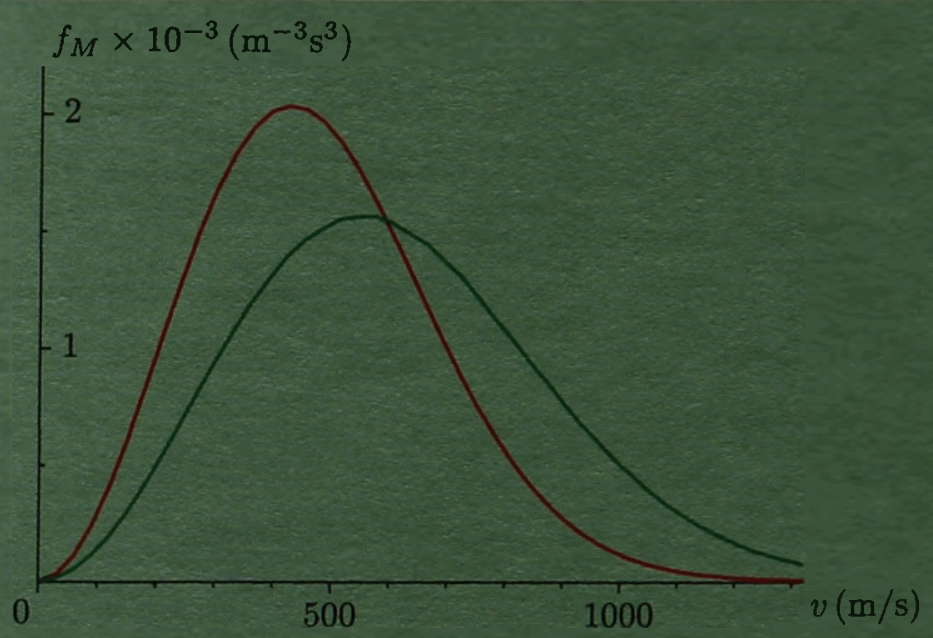
\includegraphics[width=0.4\linewidth]{mai_fig048.png}
   \captionof{figure}{Maxwellovo rozdělení rychlostí molekul dusíku pro teploty \(T_1 = 
                      \SI{300}{\kelvin}\) a \(T_2 = \SI{300}{\kelvin}\).
   \cite[s.~243]{Musilova2009MA1}
   \label{mai:fig048}}
  \par}
  
  Dokážete vyložit, proč jsme zvolili za \(\Delta\Omega\) celý objem slupky? Počítáme totiž 
  pravděpodobnost, že koncový bod vektoru rychlosti molekuly leží, zhruba řečeno, v kterémkoli 
  elementárním kvádříku \(\Delta v_x\Delta v_z\Delta v_z\) obsaženém ve slupce. A ta je součtem 
  pravděpodobností odpovídajících všem kvádříkům vytvářejícím slupku. Jedná se o pravděpodobnosti 
  navzájem neslučitelných jevů (pohybuje-li se molekula v jednom směru, nepohybuje se v jiném). 
  Hustota této pravděpodobnosti se nazývá \textbf{Maxwellovo rozdělení rychlostí}. Na rozdíl od 
  Gaussova rozdělení, popisujícího hustotu pravděpodobnosti pro jednotlivé složky rychlosti, je 
  nesymetrická vlivem faktoru \(v^2\). Obrázek \ref{mai:fig048} ukazuje funkci \(f_M(v)\) pro dvě 
  různé teploty \(T_2 > T_1\). Důležité hodnoty spjaté s tímto rozdělením jsou 
  \textbf{nejpravděpodobnější rychlost} \(v_p\), \textbf{střední rychlost} \(\langle v \rangle\) a 
  \textbf{střední kvadratická rychlost} \(\langle v^2 \rangle\). Platí
  \begin{align*}
    \der{f_M}{v}        &= 0\, \longrightarrow v_P = \sqrt{\dfrac{2kT}{m}},                      \\
    \langle v \rangle   &= \int_{-\infty}^{\infty}vf_M(v)\dd{v} = \sqrt{\dfrac{8kT}{\pi m}},     \\
    \langle v \rangle^2 &= \int_{-\infty}^{\infty}v^2f_M(v)\dd{v} = \dfrac{3kT}{m}.
  \end{align*}
\normalsize
\end{example}
      %---------------------------------------------------------------
  
  \section{Náhoda a zpracování měření}\label{mai:IchapIIIsecIV}
    \subsection{Součet a součin náhodných veličin}
      Nyní vyřešíme ještě jeden důležitý problém. Víme již, že veličinu \(Y = f(X)\) lze popsat 
      stejnými pravděpodobnostmi jako veličinu \(X\). V řadě případů je však náhodná veličina \(Y\) 
      funkcí několika náhodných veličin \(X_1, X_2, \ldots, X_s\). Každá z nich má nějaké 
      rozdělení. Jaké potom bude rozdělení veličiny \(Y\)? Rozebereme jen dvě základní situace, z 
      nichž je ovšem možné „poskládat“ řadu případů složitějších. Půjde o situace, kdy náhodná 
      veličina bude součtem nebo součinem dvou náhodných veličin, pro jednoduchost značení 
      například \(U\) a \(V\), tedy \(Y = U + V\), \(Z = U \cdot V\). Předpokládejme nejprve, že 
      veličiny \(U\) a \(V\) jsou zcela nezávislé, tj. hodnoty veličiny \(U\) nejsou nijak 
      ovlivněny hodnotami veličiny \(V\) a naopak. Dejme tomu, že \(U\) a \(V\) mají rozdělení
      \begin{equation*}
        \left\lbrace (u_1, p_1), \ldots, (u_k, p_k) \right\rbrace, \qquad
        \left\lbrace (v_1, q_1), \ldots, (v_\ell, v_\ell) \right\rbrace
      \end{equation*}
      Veličiny \(Y = U + V\), resp. \(Z = U \cdot V\) tedy mohou nabývat hodnot \(\lbrace u_i + 
      v_\alpha\rbrace\), resp. \(\lbrace u_i v_\alpha\rbrace\) s pravděpodobnostmi \(p_iq_\alpha\). 
      Jevy \uv{Veličina \(U\) nabude hodnoty \(u_i\)} a \uv{veličina \(V\) nabude hodnoty 
      \(v_\alpha\)} jsou totiž nezávislé. Rozdělení veličin \(Y\) a \(Z\) je 
      \begin{equation*}
        \lbrace (u_i +v_\alpha, p_iq_\alpha)\rbrace,\, \text{resp.}\,
        \lbrace(u_iv_\alpha, p_iq_\alpha)\rbrace,\qquad 1\leq i\leq k,\quad 1\leq\alpha\leq\ell,
      \end{equation*}
      Pro jejich střední hodnoty dostáváme
      \begin{align*}
        \langle y \rangle 
          &= \sum_{i=1}^{k}\sum_{\alpha=1}^{\ell}(u_i + v_\alpha)p_iq_\alpha
           = \sum_{i=1}^{k}u_ip_i\left(\sum_{\alpha=1}^{\ell}q_\alpha\right) + 
             \sum_{\alpha=1}^{\ell}v_\alpha q_\alpha\left(\sum_{i=1}^{k}p_i\right)  \\
          &= \sum_{i=1}^{k}u_ip_i + \sum_{\alpha=1}^{\ell}v_\alpha q_\alpha         \\
        \langle z \rangle 
          &= \sum_{i=1}^{k}\sum_{\alpha=1}^{\ell}(u_i \cdot v_\alpha)p_iq_\alpha
           = \left(\sum_{i=1}^{k}u_ip_i\right)
             \left(\sum_{\alpha=1}^{\ell}v_\alpha q_\alpha\right) 
           = \langle u \rangle \langle v \rangle.
      \end{align*}
      Střední hodnota součtu, resp. součinu náhodných veličin je tedy součtem, resp. součinem jejich
      středních hodnot. Pro součet náhodných veličin platí tento výsledek i v případě, když nebudou
      nezávislé. V tak jednoduchý závěr jsme snad ani nedoufali! Hned uvidíme, jak jej lze využít.
      
      %--Jak číst výsledky studentské ankety aneb není průměr jako průměr----------
      % !TeX spellcheck = cs_CZ
\wikitextrule
\begin{example}\label{mai:exam071}
  \textbf{Jak číst výsledky studentské ankety aneb není průměr jako průměr}\newline\small
  Každý semestr na Masarykově univerzitě se uzavírá vyhodnocením velmi užitečné studentské ankety v 
  Informačním systému MU. Studenti hodnotí na jedenáctihodnotové stupnici (nula až deset bodů) 
  několik položek pro každý studijní předmět (obtížnost, zajímavost, srozumitelnost výkladu, 
  přístup učitele, rozmanitost literatury) a mohou doplnit i slovní komentáře. Na ty se učitelé 
  těší nejvíce, neboť díky anonymitě pisatelů se tak o sobě mohou dovědět leccos zajímavého. 
  Všimneme si však statistického zpracování ankety. U každého předmětu je pro danou položku 
  vypočtena průměrná bodová hodnota odpovědí a vyznačena na téže jedenáctihodnotové stupnici. Pro 
  porovnání je na stupnici vyznačen i takzvaný „fakultní průměr“. Každý přednášející může vidět svá 
  hodnocení a hodnocení svých kolegů, kteří mu vedou cvičení. Děkan má přístupové právo k celé
  statistice, a tak může porovnávat. Jednoho deštivého večera přestalo děkana bavit vyplňování 
  rektorátních formulářů a začal si výsledky ankety prohlížet. Zajímala jej zejména položka 
  „srozumitelnost výkladu“. Řekl si, že všem učitelům, kteří v této položce budou hodnoceni 
  nadprůměrně, zvýší osobní ohodnocení. Soubor předmětů je veliký, a tak děkan klikal a klikal. 
  Zjišťoval, že u veliké většiny předmětů leží průměrné hodnocení srozumitelnosti nad fakultním 
  průměrem. Jeho pocity byly smíšené. Na jedné straně se radoval, jakými jsou jeho podřízení 
  dobrými pedagogy, na druhé straně trnul, kolik to bude stát. Snad aby se raději vrátil 
  k protivným formulářům. Najednou v něm zahlodalo podezření i naděje, že není všechno v pořádku. 
  Jak je možné, že většina hodnocení leží nad průměrem? Kladné a záporné odchylky by se přece měly 
  kompenzovat. Zavolal proto na koberec proděkana pro informační technologie, aby se jej zeptal, co 
  je to „fakultní průměr“. Proděkan odpověděl takto: Máme soubor \(K\) předmětů \(\lbrace 
  X_\alpha\rbrace\), \(\alpha = 1, \ldots, K\). V předmětu \(X_\alpha\) vyplnilo anketu 
  \(N_\alpha\)  studentů, jednotlivé hodnoty odpovědí pro danou položku (srozumitelnost výkladu) 
  byly označeny \(\lbrace x_{\alpha,j}\rbrace\), \(j = 1, \ldots, N_\alpha\). Celkem přirozeně 
  předpokládáme, že váha odpovědi každého studenta je stejná, nezávisle na předmětu. Tato váha je
  rovna převrácené hodnotě celkového počtu studentů, kteří vyplnili anketu, tj. \(w = N^{-1}\), \(N 
  = N_1 + \ldots + N_k\). Fakultní průměr je proto dán vzorcem
  \begin{equation*}
    \langle x \rangle 
      = \sum_{\alpha=1}^{K}\sum_{j=1}^{N_\alpha}wx_{\alpha,j} 
      = \dfrac{1}{N}\sum_{\alpha=1}^{K}\left(\sum_{j=1}^{N_\alpha}x_{\alpha,j}\right)
      = \dfrac{1}{N}\sum_{\alpha=1}^{K}A_\alpha,
  \end{equation*}
  kde jsme označili \(A_\alpha = \sum_{j=1}^{N_\alpha}x_{\alpha,j}\). Děkan chvíli přemýšlel a 
  pravil: To vypadá docela logicky. Neměli bychom však počítat fakultní průměr tak, že vezmeme 
  průměrné hodnoty pro každý předmět a vypočteme jejich aritmetický průměr? Pak bychom dostali
  \begin{equation*}
    \langle \overline{x} \rangle
      = \dfrac{1}{K}\sum_{\alpha=1}^{K}\langle x_{\alpha}\rangle
      = \dfrac{1}{K}\sum_{\alpha=1}^{K}
        \left(\dfrac{1}{N_\alpha}\sum_{j=1}^{N_\alpha}x_{\alpha,j}\right)
      = \dfrac{1}{K}\sum_{\alpha=1}^{K}\dfrac{A_\alpha}{N_\alpha}.
  \end{equation*}
  Tento závěr se akademickým funkcionářům na první pohled nijak zvlášť nelíbil. Bylo totiž jasné, 
  že náhodné veličiny \(X_1, \ldots, X_k\) mají odlišná rozdělení. No jo, řekli si oba, musíme 
  počítat. My už ale počítat nemusíme, neboť jsme takový problém před chvílí vyřešili obecně. 
  Zjistili jsme totiž, že střední hodnota součtu náhodných veličin je rovna součtu středních 
  hodnot, bez ohledu na konkrétní rozdělení každé z veličin. Definujeme-li tedy náhodnou veličinu 
  \(Y\) jako aritmetický průměr veličin \(X_\alpha\), tj.
  \begin{align*}
    Y &= \dfrac{1}{K}\left(X_1 + \ldots + X_K\right),  \\
    \shortintertext{dostaneme}
    \langle y \rangle &= \dfrac{1}{K}\left(\langle x_1 \rangle +\ldots+\langle x_K \rangle\right).
  \end{align*}
  Tento výsledek se shoduje s hodnotou \(\langle \overline{x} \rangle\), kterou pro výpočet 
  „fakultního průměru“ navrhl děkan. Vypočteme-li součet odchylek hodnot \(\langle x_\beta 
  \rangle\) od \(\langle y \rangle\), dostaneme skutečně nulu:
  \begin{equation*}
    \sum_{\beta =1}^{K}\left(\langle x_\beta \rangle - \langle y \rangle\right)
      = \sum_{\beta =1}^{K}\left(\dfrac{A_\beta}{N_\beta} 
      - \dfrac{1}{K}\sum_{\alpha=1}^{K}\langle x_\alpha \rangle\right)
      = 0.
  \end{equation*}
  Zkusme se ještě zamyslet nad tím , jak použití „špatného“ fakultního průměru zkreslilo výsledky a 
  proč. Vypočtěme si rozdíl \(\Delta = \langle \overline{x} \rangle - \langle x \rangle\):
  \begin{equation*}
    \Delta = \langle \overline{x} \rangle - \langle x \rangle 
      = \dfrac{1}{K}\sum_{\alpha=1}^{K}\langle x_\alpha \rangle
      - \dfrac{1}{N}\sum_{\alpha=1}^{K}A_\alpha
      = \dfrac{1}{K}\sum_{\alpha=1}^{K}\langle x_\alpha \rangle
      - \dfrac{1}{N}\sum_{\alpha=1}^{K}N_\alpha\langle x_\alpha \rangle
      = \dfrac{1}{K}\sum_{\alpha=1}^{K}\langle x_\alpha\rangle\left(1 - K\dfrac{N_\alpha}{N}\right).
  \end{equation*}
  Platí přitom
  \begin{equation*}
    \sum_{\alpha=1}^{K}\left(1 - K\dfrac{N_\alpha}{N}\right) = 0.
  \end{equation*}
  Pokud by byl počet studentů, kteří vyplnili anketu, ve všech předmětech stejný, tj. \(N_\alpha = 
  \dfrac{N}{K}\) , byla by odchylka \(\Delta\) podle očekávání nulová. Stejná situace by nastala, 
  kdyby byly shodné všechny průměrné hodnoty \(\langle x_\alpha \rangle\). Je-li odchylka 
  \(\Delta\) kladná, je „nesprávný“ fakultní průměr \(\langle x \rangle\) nižší než \(\langle 
  \overline{x} \rangle\). Proto hodnocení jednotlivých předmětů vypadají příznivěji, právě tak, jak 
  to zjistil děkan. Odchylku \(\Delta\) posouvají do kladných hodnot předměty, které hodnotilo málo 
  studentů, a předměty, které měly vysoké hodnocení. Dobře je to vidět na příkladu dvou předmětů, 
  tj. pro \(K = 2\), kde vychází
  \begin{equation*}
    \Delta = \langle \overline{x} \rangle - \langle x \rangle 
           = \dfrac{N_2 - N_1}{2(N_2+N_1)}\left(\langle\overline{x}\rangle-\langle x\rangle\right).
  \end{equation*}
  
  Pro \(N_1\ll N_2\) a \(\langle x_1 \rangle  \gg \langle x_2 \rangle \) bude rozdíl \(\Delta\) 
  skoro polovina hodnoty \(\langle x_1 \rangle\)! U volitelných specializovaných předmětů, které si 
  vybírají jen poměrně malé počty studentů, kteří navíc mají o předmět opravdový zájem a hodnotí 
  jej proto většinou vyšším počtem bodů, je splněno obojí (malý počet hodnotících a vysoké bodové
  hodnocení). Je vidět, že při nesprávně zvoleném výpočtu srovnávací hodnoty (fakultního průměru) 
  mohou právě předměty, jejichž statistický význam je spíše okrajový, ovlivnit celkové hodnocení.
\normalsize
\end{example}
      %----------------------------------------------------------------------------
      
      Pro střední hodnotu součtu a součinu nezávislých náhodných veličin jsme získali velmi
      jednoduché výsledky:
      
      \adjustbox{minipage=[c]{\textwidth}}{%
        \begin{equation}\label{mai:eq070}
          \langle u + v \rangle = \langle u \rangle + \langle v \rangle\qquad
          \langle uv \rangle    = \langle u \rangle \langle v \rangle.
        \end{equation}
      }
      
      Dokážeme také určit rozptyl veličin \(Y = U + V\) a \(Z = U\cdot V\)? Pro rozptyl každé 
      náhodné veličiny platí obecný vztah (\ref{mai:eq061}). Použijeme jej pro naše konkrétní 
      případy:
      \begin{align*}
        D(U + V) &= \langle (u + v)^2 \rangle - \langle u + v \rangle^2 
                  = \langle u^2 + 2uv + v^2 \rangle - \left(\langle u \rangle^2 +
                    \langle 2uv \rangle + \langle v^2 \rangle\right)                        \\
                 &= \left(\langle u^2\rangle - \langle u \rangle^2\right)
                  + \left(\langle v^2\rangle - \langle v \rangle^2\right) = D(U) + D(V).
      \end{align*}
      Pro rozptyl náhodné veličiny \(Z = U \cdot V\) dostaneme
      \begin{align*}
        D(Z)  &= \langle z^2\rangle - \langle z \rangle^2 
               = \langle u^2\rangle\langle v^2\rangle - \langle u \rangle^2 \langle v \rangle^2  \\
              &= \left[D(U) + \langle u^2\rangle\right]\left[D(V) + \langle v^2\rangle\right]
               - \langle u \rangle^2 \langle v \rangle^2                                         \\
              &= D(U)D(V) + \langle u \rangle^2D(V) + \langle v \rangle^2D(U).
      \end{align*}
      Pak
      \adjustbox{minipage=[c]{\textwidth}}{%
        \begin{equation*}
          \dfrac{D(z)}{ \langle z \rangle^2} = \dfrac{D(U)}{ \langle u \rangle^2} \cdot
            \dfrac{D(V)}{ \langle v \rangle^2} + \dfrac{D(U)}{ \langle u \rangle^2} +
            \dfrac{D(v)}{ \langle v \rangle^2}.
        \end{equation*}
      }
      Při výpočtu jsme využili vztahu (\ref{mai:eq061}) a vztahů (\ref{mai:eq070}) pro střední 
      hodnotu součtu a součinu náhodných veličin. Pokud mají veličiny \(U\) a \(V\) shodný rozptyl 
      \(D(U) = D(V) = D\), pak je \(D(U + V) = 2D\). V případě součtu s veličin \(Y = X_1 + \cdots 
      + X_s\) se shodným rozptylem \(D\) resp. směrodatnou odchylkou \(\sigma\) dostáváme
      \begin{equation*}
        D(Y) = sD  \Rightarrow \sigma(y) = \sqrt{s}\sigma.
      \end{equation*}
      Znovu připomeňme, že všechny vztahy týkající se součtu a součinu náhodných veličin, které
      jsme zatím získali, platí za předpokladu, že výchozí veličiny, které sčítáme nebo násobíme, 
      jsou nezávislé.
      
      Aniž bychom se podrobněji zabývali vlastnostmi rozdělení závislých veličin, definujeme pro
      ně charakteristiky, které tuto závislost popisují. Nechť \(U\) a \(V\) jsou dvě libovolně 
      náhodné veličiny, ne nutně nezávislé. Míru jejich závislosti určují veličiny
      \begin{equation}\label{mai:eq071}
        \sigma_{uv} = \langle (u - \langle u \rangle) (v - \langle v \rangle) \rangle, \qquad
        \varrho_ {uv}=\dfrac{\sigma(u)}{\sqrt{D(U)D(V)}} = \dfrac{\sigma(u)}{\sigma{D(u)\sigma(v)}}
      \end{equation}
      zvané \textbf{kovariance} a \textbf{korelační koeficient} veličin \(U\) a \(V\). Platí 
      \(\varrho(uv) \leq 1\). Pro nezávislé veličiny vychází \(\sigma(uv) = 0\) a \(\varrho(uv) = 
      0\).
      
      %-- Rozptyl při Bernoulliově pokusu-----------------------------
      % !TeX spellcheck = cs_CZ
\begin{mdframed}[style=mdexam]
  \begin{example}\label{mai:exam072}
    \textbf{Rozptyl při Bernoulliově pokusu}\newline
    V příkladu \ref{mai:exam066} jsme se zajímali o střední hodnotu veličiny \(X\) definované jako
    počet zdarů při \(n\) opakováních Bernoulliova pokusu. Řekli jsme si, že střední hodnota této
    veličiny je \(np\) s tím, že důkaz lze provést přímo na základě definičního vztahu pro střední
    hodnotu matematickou indukcí. Výpočet rozptylu z definičního vztahu bychom jistě snadno dokázali
    zahájit, horší by však bylo dovést jej do konce. Stačí se podívat na začátek výpočtu
    \begin{align*}
      D(X) &= \sum_{j=0}^n \left(x_j - \langle x \rangle\right)^2p_j             \\
           &= \sum_{j=0}^n \left(j - np\right)^2\binom{n}{j}p^j(1 - p)^j,
    \end{align*}
    a nepochybujeme o tom, že tuto sumu nedokážeme spočítat snadno. Protože již však umíme zacházet
    se součtem náhodných veličin, můžeme využít účinného triku. Veličinu \(X\) si představíme jako
    součet
    \begin{equation*}
      X = U_1 + U_2 + \cdots + U_n,
    \end{equation*}
    kde každá z veličin \(U_j\) může nabývat dvou hodnot. Jedničky v případě, že při \(j\)-tém
    opakování pokusu nastal zdar, a nuly v případě, že nastal nezdar. Součet všech veličin \(U_j\)
    pro \(j = 1\) až \(j = n\) pak skutečně znamená celkový počet zdarů při \(n\) opakováních
    pokusu. Jestliže si uvědomíme, že pravděpodobnost zdaru při kterémkoli z opakování je \(p\) a
    pravděpodobnost nezdaru \((1 - p)\), ihned vidíme, že rozdělení každé z veličin \(U_j\) má tvar
    \(\lbrace(1, p), (0, 1 - p)\rbrace\). Platí tedy
    \begin{equation*}
      \langle u_j\rangle = 1\cdot p + 0 \cdot (1 - p) = p,
    \end{equation*}
    \begin{align*}
      D = D(U_j) &= \left( 1 - \langle u_j\rangle\right)^2p 
                  + \left( 0 - \langle u_j\rangle\right)^2(1 - p)   \\
                 &= p(1 - p)^2 + p^2(1 - p) = p(1 - p).
    \end{align*}
    Každé dvě veličiny \(U_i\), \(U_j\) jsou nezávislé, neboť jednotlivá opakování pokusu jsou
    nezávislá. Střední hodnota jejich součtu je: tedy \(np\) (a to souhlasí s informací v příkladu
    \ref{mai:exam066}) a pro rozptyl jejich součtu platí
    \begin{equation*}
      D(X) = nD = np(1 - p).
    \end{equation*}
    Celkově tedy dostáváme
    \begin{equation*}
      \langle x \rangle = np, \; \sigma(x) = \sqrt{np(1 - p)}.
    \end{equation*}
  \end{example}
\end{mdframed}
      %---------------------------------------------------------------
      
      %-- Rozptyl aritmetického průměru-------------------------------
      % !TeX spellcheck = cs_CZ
\begin{mdframed}[style=mdexam]
  \begin{example}\label{mai:exam073}
    \textbf{Rozptyl aritmetického průměru}\newline
    Již v úvodu odstavce o náhodných veličinách jsme konstatovali, že opakujeme-li v nezměněných
    podmínkách měření jisté fyzikální veličiny (délka závěsu kyvadla, proud procházející vodičem,
    napětí na vodiči, atd.), budeme díky náhodným vlivům dostávat pokaždé poněkud jiný výsledek.
    Říkáme, že měření je zatíženo náhodnými chybami. Výsledek získaný při každém opakování lze
    interpretovat jako hodnotu náhodné veličiny. Dejme tomu, že jsme provedli uměření fyzikální
    veličiny \(X\) a získali hodnoty \(x_1\) až \(x_n\) . V praktické situaci budou tyto hodnoty
    většinou navzájem různé, nemusí tomu tak však nutně být. Fyzikální veličinu chceme ovšem
    reprezentovat jediným údajem, a tím bude její střední hodnota, tj.
    \textbf{aritmetický průměr}
    \begin{equation*}
      \langle x \rangle = \dfrac{x_1 + x_2 + \cdots + x_n}{n}.
    \end{equation*}
    Rozptyl veličiny \(X\) je dán vztahem
    \begin{align*}
      D &= D(X)                                                             \\
        &= \dfrac{\left(x_1 - \langle x \rangle\right)^2 + 
                  \left(x_2 - \langle x \rangle\right)^2 + \cdots +
                  \left(x_n - \langle x \rangle\right)^2}{n}.
    \end{align*}
    Víme, že směrodatná odchylka \(\sigma( x ) = \sqrt{D(X)}\) určuje, nakolik jsou jednotlivé
    výsledky měření v průměru odchýleny od střední hodnoty, charakterizuje tedy přesnost každého
    opakování měření. Podívejme se na celou úlohu z jiné strany: Představme si, že sledujeme \(n\)
    po dvou nezávislých náhodných veličin \(X_1\) až \(X_n\) se shodnou střední hodnotou \(\langle
    x_j \rangle = \langle x \rangle\) a shodnou směrodatnou odchylkou \(\sigma(x_j) = \sqrt{D},\, 1
    \leq j \leq n\). Aritmetický průměr těchto veličin,
    \begin{equation*}
      \langle \Xi \rangle = \dfrac{X_1 + X_2 + \cdots + X_n}{n}.
    \end{equation*}
    je tedy rovněž náhodnou veličinou. Pro jeho střední hodnotu, rozptyl a směrodatnou odchylku
    platí
    \begin{align*}
      \langle \xi \rangle 
                  &= \dfrac{n\langle x \rangle}{n}, \\
      D(\Xi)      &= \dfrac{1}{n^2}\cdot D(X_1 + \cdots + X_n)=\dfrac{nD^2}{n^2}=\dfrac{D}{n}, \\
      \sigma(\xi) &= \dfrac{\sigma(x)}{\sqrt{n}}.
    \end{align*}
  \end{example}
\end{mdframed}
      %---------------------------------------------------------------
      
      Můžeme tedy říci, že aritmetický průměr všech výsledků měření dané fyzikální veličiny je
      \(\sqrt{n}\)-krát přesnější než jednotlivý výsledek měření. Jakkoli se toto konstatování zdá 
      intuitivně zřejmé, je třeba je používat s opatrností.
      
      Především je třeba mít na mysli, co toto konstatování znamená. Jeho charakter je totiž
      opět jen pravděpodobnostní. Jestliže jsou jednotlivá měření prováděna za stejných podmínek,
      jsou rozdělení veličin \(X_1\) až \(X_n\) funkcemi téhož typu. Tyto veličiny mají také 
      stejnou střední hodnotu \(\langle x \rangle\) a směrodatnou odchylku \(\sigma\). Také 
      pravděpodobnost, že při měření padne hodnota veličiny \(X_j\) do intervalu \((\langle x 
      \rangle - \sigma, \langle x \rangle + \sigma)\), je pro všechna \(j\) prakticky stejná. 
      Označme ji \(P_\sigma\).  Se stejnou pravděpodobností nabude aritmetický průměr \(\Xi\) 
      hodnoty v intervalu určeném svou směrodatnou odchylkou. Ta je však \(\sqrt{n}\)-krát menší. V 
      tomto smyslu jsou hodnoty aritmetického průměru \uv{\(\sqrt{n}\)-krát méně rozptýleny} kolem 
      střední hodnoty \(\langle\xi \rangle\) než hodnoty náhodných veličin \(X_j\) kolem svých 
      středních hodnot \(\langle x \rangle\).
      
      Dalším problémem může být splnění výchozích předpokladů, které vedly ke vztahu pro
      směrodatnou odchylku aritmetického průměru. Ukážeme to na následujícím příkladu.
      
      %-- Jak přesně lze změřit čínského císaře?----------------------
      % !TeX spellcheck = cs_CZ
\wikitextrule
\begin{example}\label{mai:exam075}
  \textbf{Ověření Ohmová zákona}\newline\small

\normalsize
\end{example}
      %---------------------------------------------------------------
      
      %-- Záhada přijímací zkoušky aneb k čemu může posloužit distribuční funkce-----
      % !TeX spellcheck = cs_CZ
\begin{mdframed}[style=mdexam]
  \begin{example}\label{mai:exam075}
    \textbf{Záhada přijímací zkoušky aneb k čemu může posloužit distribuční funkce?}\newline
    Mohlo by se zdát, že distribuční funkce je jen teoretický pojem a že v praktických situacích ji
    těžko využijeme. Podstatné je přece pravděpodobnostní rozdělení náhodné veličiny a distribuční
    funkce je z něj jen jaksi odvozena sčítáním pravděpodobností (u diskrétního rozdělení) nebo
    integrací (u rozdělení spojitého). Přesvědčíme se, že existují velmi realistické případy, kdy
    distribuční funkce přináší věrohodnější informaci o náhodné veličině než samotné rozdělení.
    
    Na Masarykově univerzitě musí každý uchazeč o studium, ať již se hlásí na přírodovědeckou,
    právnickou, lékařskou či jinou fakultu, absolvovat Test studijních předpokladů. Jedná se o
    všeobecný test, zaměřený na zjišťování úrovně všech schopností uchazeče, které jsou potřebné pro
    univerzitní studium, například analytického myšlení, verbálních schopností, numerického myšlení,
    geometrické představivosti, atd. Pro nás však v tu to chvíli není podstatný obsah testu, ale
    způsob zpracování jeho výsledků a vyhodnocení pořadí uchazečů. Test skládá kolem třiceti tisíc
    studentů. Není tedy možné technicky zajistit, aby proběhl v jediné variantě v jednom dni. K
    dispozici je proto osm variant testu, každou variantu řeší tři až čtyři tisíce studentů. Test má
    \num{80} otázek, základním údajem pro zpracování jeho výsledků je počet správných odpovědí
    každého studenta. Pokud bychom označili jako \(i\) počet správných odpovědí (\(i \in\lbrace0, 1,
    2, \ldots, 80\rbrace\)) v kterékoli variantě a \(\mathcal{N}_i\) počet studentů, kteří dosáhli
    právě \(i\) správných odpovědí, dostaneme náhodnou veličinu \(X_i\), kterou bychom mohli nazvat
    „počet správných odpovědí“, pro celou univerzitu. Její rozdělení by mělo tvar
    \begin{equation*}
      \lbrace(i,p_i)\rbrace,\quad\text{kde}\qquad p_i = \dfrac{\mathcal{N}_i}{\mathcal{N}}, \quad
      \mathcal{N} = \sum_{i=0}^{80}\mathcal{N}_i
    \end{equation*}
    A zde je malý „kámen úrazu“. A by bylo možné sestavit opravdu „univerzální pořadí“, musely by
    být všechny varianty testu ekvivalentní z hlediska obtížnosti. To znamená, že kdyby kterýkoli
    student vyplnil za stejných podmínek všechny varianty, dosáhl by v každé z nich stejného počtu
    správných odpovědí s pravděpodobností velmi blízkou jedné. Skutečnost je však principiálně
    taková, že u sebelépe promyšleného a sestaveného testu se jednotlivé varianty budou mírně, v
    rámci statistických, a tedy již neodstranitelných, odchylek lišit. Tato odlišnost se nepozná
    předem, ale až po zpracování výsledků všech variant. Použít pro stanovení pořadí uchazečů
    rozdělení náhodné veličiny \(X\) \emph{= počet správných odpovědí je tedy nespravedlivé}.
    Student, který řešil variantu „statisticky obtížnější“, by v pořadí skončil s horším umístěním,
    než student, který je stejně schopný, avšak měl to štěstí, že na něj připadla varianta
    „statisticky méně obtížná“. Skutečně, kdybychom sestavili grafy rozdělení náhodných veličin
    \(X^{(\alpha)}\) \emph{= počet správných odpovědí v \(\alpha\)-té variantě},
    \begin{equation*}
      \lbrace(i,p_i^{(\alpha)})\rbrace,\quad\text{kde}\; 
      p_i^{(\alpha)} = \dfrac{\mathcal{N}_i^{(\alpha)}}{\mathcal{N}^{(\alpha)}}, \quad
      \mathcal{N}^{(\alpha)} = \sum_{i=0}^{80}\mathcal{N}_i^{(\alpha)}
    \end{equation*}
    zjistili bychom, že se mírně liší. (V předchozím zápisu značí \(\mathcal{N}_i^{(\alpha)}\) počet
    studentů, kteří odpověděli správně na \(i\) otázek \(\alpha\)-té varianty
    \(\mathcal{N}^{(\alpha)}\) je počet všech studentů, kteří tuto variantu řešili.) Střední hodnoty
    i mediány náhodných veličin se i při vynikající shodě obtížnosti všech variant mohou lišit v
    rozmezí jedné až dvou správných odpovědí. A s ohledem na skutečnost, že každou variantu řeší
    obrovský počet studentů, až čtyři tisíce, je zřejmé, že tento rozdíl může poněkud „zamíchat
    “pořadím, zejména v blízkosti mediánu, kde se týká třeba i tří stovek studentů v každé variantě.
    Situaci dokládá obrázek \ref{mai:fig049}. Jak tedy zařídit, abychom dostali spravedlivé pořadí?
    Jediný rozumný způsob, jak minimalizovat vliv statistických odchylek obtížnosti jednotlivých
    variant, je nehodnotit studenty podle absolutního počtu správných odpovědí, ale nějak je
    porovnat mezi sebou. Budeme při tom předpokládat, že rozložení schopností studentů je ve všech
    osmi skupinách, které řeší osm daných variant, stejné. Řeknete si - zase nějaké další
    předpoklady. To je jako z bláta do louže. Předpoklad o stejném rozložení schopností studentů v
    tak velkých skupinách, jako jsou ty naše, je však mnohem realističtější než předpoklad o
    dokonalé shodě obtížnosti variant testu. Budeme se jej proto držet. Každému studentovi
    přisoudíme číslo, které informuje o tom, kolik řešitelů dané varianty bylo horších nebo stejně
    dobrých jako on, tj. mělo nižší nebo stejný počet správných odpovědí. Z matematického hlediska
    to znamená přejít v každé variantě od rozdělení k distribuční funkci. Věnujme se nyní tomuto
    přepočtu podrobněji jak pro diskrétní rozdělení náhodné veličiny \(X^{(\alpha)}\), které
    odpovídá skutečné situaci, tak pro zajímavost i pro rozdělení spojité. V dalším budeme vždy
    zpracovávat výsledky jedné varianty, upustíme proto od vyznačování indexu \(\alpha\).

    {\centering
    \captionsetup{type=figure}
    \luafigure[0.8]{mai_fig049.png}
    \captionof{figure}{Rozdělení pro dvě varianty testu,
    \cite[s.~252]{Musilova2009MA1}
    \label{mai:fig049}}
    \par}
    
    \textbf{Diskrétní rozdělení}
      \begin{itemize}
        \item \emph{Zadání:} Skupina \(N\) studentů řeší jednu variantu testu. Test má \(Q\) otázek.
              Za každou správnou odpověď je přidělen jeden výchozí bod. Získáváme rozdělení
              \begin{gather*}
                \left\lbrace\left(i, \dfrac{N_i}{N} \right)\right\rbrace, \;
                i\in\lbrace0, 1, 2, \ldots, Q\rbrace, \;
                \sum_{i=0}^{Q}N_i = N 
              \end{gather*}
              kde \(i\) je počet výchozích bodů a \(N_i\) počet studentů, kteří získali \(i\) bodů.
              Distribuční funkce tohoto rozdělení
              \begin{gather*}
                F(x) = \dfrac{1}{N}\sum_{i=0}^{j}N_i\;\text{ pro }\;
                j\leq x < j+1, \; x\in\left[0,\infty\right)
              \end{gather*}
              Pro uchazeče, který získal \(j\) bodů, mají význam následující hodnoty:
              \begin{itemize}
                \item \(F(x)    x \in \left[j, j+1\right)\): poměrný počet uchazečů, kteří získali
                      počet výchozích bodů nižší nebo shodný s daným uchazečem,
                \item \(NF(x)   x \in \left[j, j+1\right)\): absolutní počet uchazečů, kteří získali
                      počet výchozích bodů nižší nebo shodný s daným uchazečem,
                \item \(100F(x) x \in \left[j, j+1\right)\): absolutní počet uchazečů, kteří získali
                      počet výchozích bodů nižší nebo shodný s daným uchazečem,
              \end{itemize}
        \item Hodnoty distribuční funkce můžeme získat z následující tabulky:
        
              {\centering
                \resizebox{0.8\textwidth}{!}{%
                \begin{tabular}{c|c}
                          interval \(x\)     &  \(NF(x)\)         \\ \hline
                  \(\left[0,1\right)\)       &  \(N_0\)           \\ 
                  \(\left[1,2\right)\)       &  \(N_0 + N_1\)     \\ 
                  \(\cdots\)                 &  \(\cdots\)        \\
                  \(\left[j,j+1\right)\)     &  \(N_0 + N_1 + \cdots + N_j\) \\ 
                  \(\cdots\)                 &  \(\cdots\) \\
                  \(\left[Q-1,Q\right)\)     &  \(N_0 + N_1 + \cdots + N_{Q-1}\) \\ 
                  \(\left[Q,\infty\right)\)  &  \(N_0 + N_1 + \cdots + N_{Q} = N\) 
                \end{tabular}}
              \par}
        \item Přepočet hodnocení uchazečů tak, aby nová stupnice byla opět v rozsahu mezi nulou a
              \(Q\) a aby nové hodnocení bylo opět celočíselné, je následující:
              \begin{equation*}
                y =QF(x), \quad 0\leq F(x) \leq 1, \Rightarrow y \in[0,Q].
              \end{equation*}
              Uchazeči se ziskem \(i\) výchozích bodů náleží hodnota \(y = QF(x)\) právě když i\(
              \in \left[i, i + 1\right)\), tj. \(y_i = Q F(i)\). Tato hodnota není obecně
              celočíselná. Zaokrouhlení se provede ve prospěch uchazeče, tedy vždy nahoru. Výsledný
              převodní vzorec je
              \begin{equation*}
                \begin{multlined}
                  \text{výchozí body } i \longrightarrow\text{ nové body }  \\ 
                  \shoveleft[1cm]Y_i: Y_i = [y_i] + 1 = [QF(i)] + 1,
                \end{multlined}
              \end{equation*} 
              kde \([a]\) značí celočíselnou část čísla \(a\), tedy například \([\num{23.05}] =
              [\num{23.48}] = [23,89] = 23\)
        \item Zaveďme novou náhodnou veličinu \(Z\) s rozdělením \(\left\lbrace(z_\alpha,
              M_\alpha)\right\rbrace\): Označme \(z_1, z_2, \ldots, z_\alpha, ...,\) \(z_S\)
              navzájem různé hodnoty ze souboru \(\lbrace Y_i\rbrace, i = 0, 1, 2, \ldots, Q\)
              řazené vzestupně. Její rozdělení udává kterákoli z následujících tabulek:

              {\centering
                \resizebox{0.9\textwidth}{!}{%
                \begin{tabular}{c|c}
                          hodnota                       &  četnost         \\
                          \hline
                  \(z_1 = Y_0 = Y_1 = \cdots Y_{i_1}\)  & \(M_1 = N_0 + N_1 + \cdots + N_{i_1}\)  \\ 
                  \(Z_2 = Y_{i_1+1} = \cdots Y_{i_2}\)  & \(M_2 = N_{i_1+1} + \cdots + N_{i_2}\)  \\ 
                  \(\cdots\)                            & \(\cdots\)                              \\
                  \(Z_S = Y_{i_{S-1}+1}=\cdots Y_{i_S}\)& \(M_S = N_{i_{S_1}+1}+\cdots+N_{i_S}\)   
                \end{tabular}}
              \par}

              {\centering
                \resizebox{0.9\textwidth}{!}{%
                \begin{tabular}{c|c}
                          hodnota                        &  četnost         \\
                          \hline
                  \(z_1 = Y_0 = Y_1 = \cdots Y_{i_1}\)   &  \(M_1 = NF(i_1)\)              \\
                  
                  \(Z_2 = Y_{i_1+1} = \cdots Y_{i_2}\)   &  \(M_2 = N[F(i_2) - F(i_1)]\)  \\ 
                  \(\cdots\)                             &  \(\cdots\)                     \\
                  \(Z_S = Y_{i_{S-1}+1}=\cdots Y_{i_S}\) & \(M_S = N[F(i_S) - F(i_{S-1})]\)   
                \end{tabular}}
              \par}
              kde \(i_1 < i_2 < \ldots < i_{S-1} < i_S, i_S = Q\) (Vzhledem k zaokrouhlování nahoru
              není žádná bodová hodnota \(Y_i\) nulová.) I když skutečné rozdělení při zpracování
              výsledků testů je diskrétní, ukažme si, jak by vypadal analogický postup u rozdělení
              spojitého, kde je početní zpracování názornější.
      \end{itemize}
    
    \textbf{Spojité rozdělení}
      \begin{itemize}
        \item \emph{Zadání:} Je dáno rozdělení četností \(n(x) \leq 0,\, x \in [0, Q]\).
        \item Normovací podmínka a distribuční funkce jsou
              \begin{equation*}
                \int_{0}^{Q}n(x)\dd{x} = N, \quad 
                F(x) = \dfrac{1}{n}\int_{0}^{x}n(\xi)\dd{\xi},                
              \end{equation*}
              kde \(0 \leq F(x) \leq 1.\)
        \item Označme \(z = QF(x)\), tedy \(z \in [0, Q]\), novou náhodnou veličinu. (Uvědomme si,
              že \(z\) je rostoucí funkcí proměnné \(x\)). Označme její rozdělení \(\nu(z)\). Její
              distribuční funkce je
              \begin{align*}
                \Phi(z) &= \int_{0}^{z}\nu(\zeta)\dd{\zeta} 
                         = \int_{0}^{x(z)}\dfrac{n(\xi)}{N}\dd{\xi}          \\
                        &= F\left(F^{-1}(z/Q)\right) 
                        = \dfrac{z}{Q}, \quad
                \nu(z) = \dfrac{1}{Q}.
              \end{align*}
        \item Rozdělení je konstantní s mediánem i střední hodnotou \(Q/2\). Takové rozdělení se
              nazývá rovnoměrné.
      \end{itemize}
  \end{example}
\end{mdframed}
      %------------------------------------------------------------------------------
      
    \subsection{Který výsledek je ten pravý?}
      První věc, kterou budete dělat ve fyzikálním praktiku, bude zjišťování průměrné hustoty 
      materiálu, z něhož je vyroben kovový váleček. Budete váleček vážit, abyste určili jeho 
      hmotnost,a měřit jeho výšku a průměr, abyste mohli vypočítat jeho objem. Hustotu stanovíte 
      jako podíl hmotnosti a objemu. Jedná se stále o jeden a týž váleček, jehož průměrná hustota 
      má za daných podmínek (stálá teplota, váleček se nedeformuje, apod.) stále stejnou „správnou“ 
      hodnotu, kterou však neznáme. (Nezná ji ani učitel v praktiku, i když se tak tváří.) Změří-li 
      hustotu válečku všichni studenti ve skupině, každý jen jednou, získá se řada různých hodnot. 
      Která z nich je ta správná? Není vyloučeno, a je to dokonce velmi pravděpodobné, že žádná. A 
      mohli bychom pomocí nich správnou hodnotu určit nebo se k ní alespoň přiblížit? Možné by to 
      bylo, pokud bychom zaručili, že všechny výsledky získané jednotlivými studenty jsou „stejně 
      hodnotné“. Znamenalo by to, že bychom museli vyloučit hrubé a systematické chyby, které by 
      vznikly třeba tak, že by někteří studenti vážili na vadných vahách, někteří by měli špatné 
      měřítko, popřípadě by odečítali údaj „zboku“, takže by byl zkreslený, nebo by se dokonce 
      zmýlili při odečítání údaje. Museli bychom také zaručit, že náhodné vlivy, které ovlivňují 
      měření, zatěžují je náhodnými chybami a v principu je nelze odstranit, byly při všech 
      měřeních stejné. U různých studentů si tím však nemůžeme být jisti (vzpomeňte si na měření 
      čínského císaře), proto budeme raději postupovat tak, že jeden pečlivý student provede větší 
      počet měření třeba výšky válečku, která je pro určení hustoty potřebná. Dejme tomu, že bude 
      měřit milimetrovým měřítkem a bude odhadovat s přesností na půl milimetru. Jeho údaje tedy 
      mohou mít tvar \SI{33.0}{\mm}, \SI{34.5}{\mm}, atd. Získá takto za stejných podmínek třeba 
      dvacet nebo i padesát hodnot, ale co teď s nimi? Jak určit hodnotu, která se bude nejvíce 
      blížit správné hodnotě výšky válečku? (Dalo by se jistě diskutovat i o tom, co je to správná 
      hodnota. Pro tuto chvíli však předpokládejme, že taková hodnota skutečně existuje, neboť 
      váleček je opravdu válcem, je vysoustružen pečlivě, přesněji, než jsme schopni jej měřit, při 
      měření se nemění teplota, váleček není dáván do lisu a deformován, ani upravován tak, že by 
      se měnila jeho hmotnost.) Předpokládejme, že správná hodnota výšky válečku je \(x\) a že 
      student naměřil hodnoty \(\lbrace x_1, X_2, \ldots, x_n\rbrace\), mezi nimiž mohou být 
      pochopitelně i některé hodnoty stejné. Odchylky jeho měření od správné hodnoty jsou
      \begin{equation*}
        \lbrace \varepsilon_1, \varepsilon_2, \ldots, \varepsilon_n\rbrace, \qquad
        \varepsilon_i = x_i - x, \qquad i = 1, 2, \ldots, n.
      \end{equation*}
      I kdybychom správnou hodnotu \(x\) znali, nedokázali bychom předpovědět, nakolik se od ní při
      jednotlivém měření odchýlíme. Můžeme, se však zajímat o to, jaká je pravděpodobnost, že
      hodnota, o kterou bude měření od správné hodnoty odkloněno, bude ležet v určitém intervalu.
      Odchylky \(\varepsilon_i\) lze totiž interpretovat jako hodnoty náhodné veličiny. Abychom 
      mohli požadované pravděpodobnosti určit, potřebujeme znát rozdělení této veličiny. Označme ji 
      \(\varepsilon\) a odpovídající hustotu pravděpodobnosti \(\mathcal{w}(\varepsilon)\). Toto 
      rozdělení je za určitých podmínek \textbf{rozdělením normálním}, splňuje tedy vztah 
      (\ref{mai:eq069}). Zkusme se o tom přesvědčit. Zvolme podmínky měření tak, aby byly ve hře 
      jen náhodné chyby způsobené \(m\) nezávislými vlivy. Každý z nich hodnotu měření
      odchýlí od \(x\) o stejně velkou hodnotu \(\alpha\), kladnou nebo zápornou, s 
      pravděpodobností \num{0.5}. Schéma této úvahy je na obrázku \ref{mai:fig050}. Výsledná 
      odchylka naměřené hodnoty \(x_i\) od hodnoty správné s jistotou leží v intervalu \((-m\alpha, 
      m\alpha)\) a může nabývat pouze hodnot celých násobků \(\alpha\). Při uplatnění jednotlivého 
      „chybového“ vlivu vzniká, jak jsme již řekli, kladná nebo záporná odchylka o velikosti 
      \(\alpha\). Vznik odchylky \(+\alpha\) nazveme zdarem, vznik odchylky \(-\alpha\) nezdarem.
      
      \begin{figure}[ht!] %\ref{mai:fig050}
        \centering
        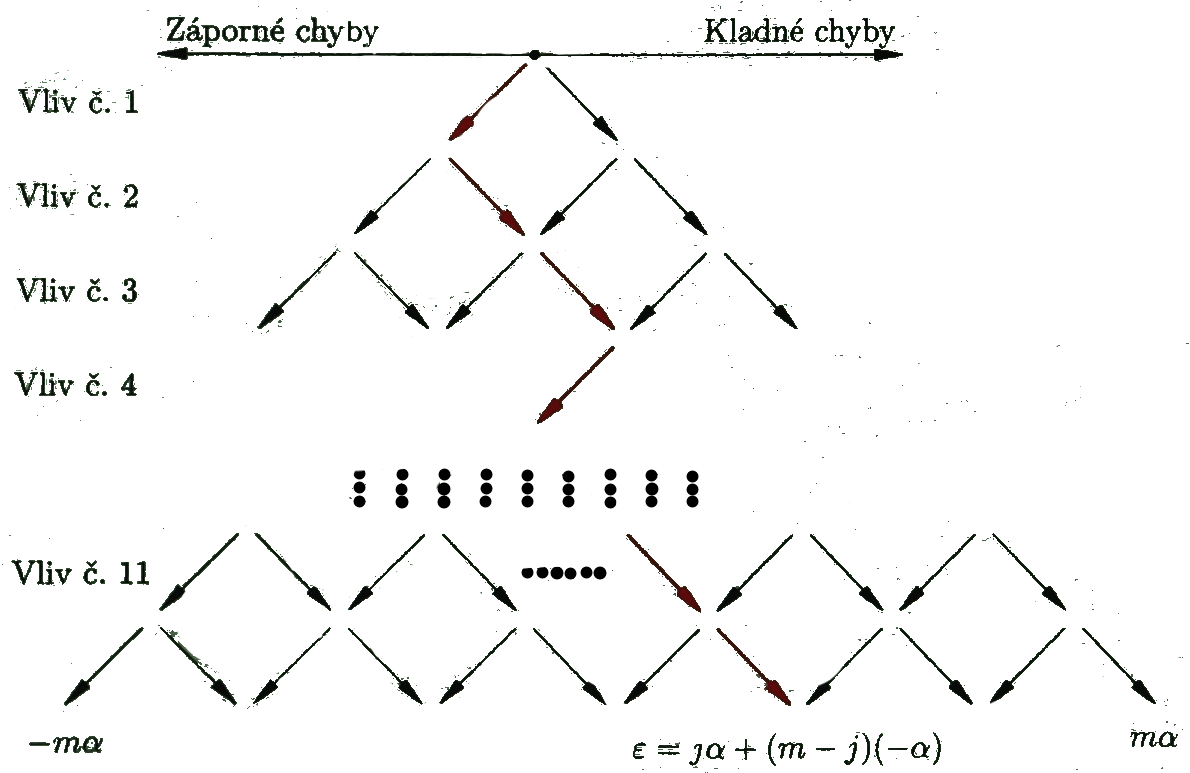
\includegraphics[width=0.6\linewidth]{mai_fig050.png}
        \caption{Vznik kladných a záporných odchylek při měření s \(m\) vlivy. 
        \cite[s.~255]{Musilova2009MA1}}
        \label{mai:fig050}
      \end{figure}
      
      Mohlo by tomu být i naopak, slova „zdar“ a „nezdar“ zde nemají svůj obvyklý význam, jde
      pouze o to, že díky nim můžeme hned uvidět souvislost s Bernoulliovým pokusem a tedy
      i s Bernoulliovým rozdělením. Při \(j\) kladných a \(m — j\) záporných odchylkách je měření od
      správné hodnoty odkloněno o
      \begin{equation*}
        j\alpha + (m - j)(-\alpha) = (2j - m)\alpha
      \end{equation*}
      s pravděpodobností
      \begin{equation*}
        p_j = \begin{pmatrix}m j\end{pmatrix}p^j(1 - p)^{m - j} = 2^{-m}.
      \end{equation*}
      Střední hodnota náhodné veličiny \(\varepsilon\) je nulová. Skutečně, v příkladu 
      \ref{mai:exam066} jsme zjistili, že střední hodnota veličiny \(Y\) nabývající hodnot \(y_j = 
      j\) s Bernoulliovým rozdělením je \(\langle y \rangle = mp\), střední hodnota veličiny \((2j 
      — m)\) a pak musí být \((2mp — m)\alpha\). Pro \(p = \num{0.5}\) je tato hodnota nulová.
      Pro velká \(m\) lze Bernoulliovo rozdělení nahradit rozdělením normálním (obr. 3.8), a proto 
      má náhodná veličina \(\varepsilon\) hustotu pravděpodobnosti tvaru (\ref{mai:eq069}), tj.
      \begin{equation*}
        \mathcal{w}(\varepsilon) = 
        \dfrac{1}{\sigma\sqrt{2\pi}}\exp\left(\dfrac{-\varepsilon^2}{2\sigma^2}\right).   
      \end{equation*}
      \begin{figure}[ht!] %\ref{mai:fig051}
        \centering
        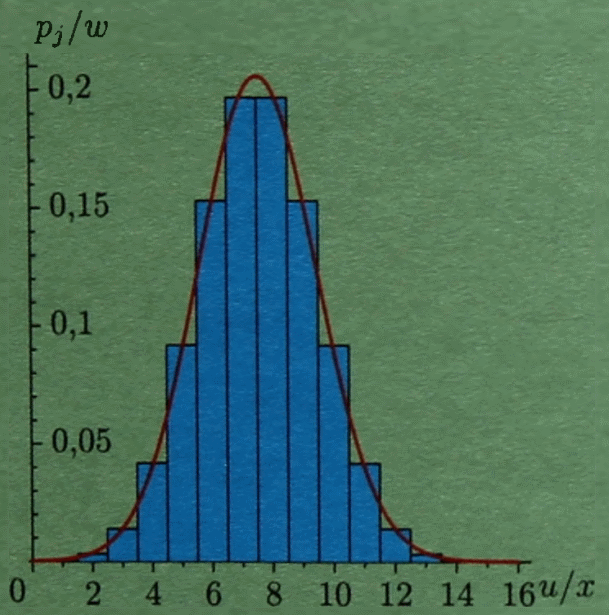
\includegraphics[width=0.4\linewidth]{mai_fig051.png}
        \caption{Normální rozdělení jako limitní případ Bernoulliova 
        \cite[s.~256]{Musilova2009MA1}}
        \label{mai:fig051}
      \end{figure}
      
      Vraťme se nyní k otázce zpracování naměřených hodnot \(\lbrace x_1, \ldots, x_n\rbrace\) 
      výšky válečku. Jejich odchylky od správné hodnoty jsou \(x_1 - x\) až \(x_n - x\). Na místě 
      neznámé správné hodnoty \(x\) si nyní představme nějakou proměnnou, označme ji 
      \(\varepsilon\). Budeme se snažit určit její hodnotu \(\varepsilon_0\) tak, aby 
      pravděpodobnost, že odchylky jednotlivých měřených hodnot od \(\varepsilon_0\) padnou 
      současně do intervalů
      \begin{equation*}
        \left(\varepsilon_1 - \dfrac{\dd{\varepsilon_1}}{2}, 
              \varepsilon_1 + \dfrac{\dd{\varepsilon_1}}{2}
        \right),
        \left(\varepsilon_2 - \dfrac{\dd{\varepsilon_2}}{2}, 
              \varepsilon_2 + \dfrac{\dd{\varepsilon_2}}{2}
        \right), \cdots,
        \left(\varepsilon_n - \dfrac{\dd{\varepsilon_n}}{2}, 
              \varepsilon_n + \dfrac{\dd{\varepsilon_n}}{2}
        \right),
      \end{equation*}
      byla maximální. Pro tuto pravděpodobnost v závislosti na \(\xi\) platí
      \begin{align}
        \dd{W} &= \dd{\mathcal{w}(\varepsilon_1)}\cdots\dd{\mathcal{w}(\varepsilon_n)}  \nonumber\\
               &= \dfrac{1}{\sigma\sqrt{2\pi}}
                  \exp\left(-\dfrac{(x_1 - \xi)^2 + \cdots + (x_n - \xi)^2}{2\sigma^2}
                      \right)\dd{\varepsilon_1}\cdots\dd{\varepsilon_n}.      \label{mai:eq072}
      \end{align}
      (Víte proč je ve vztahu (\ref{mai:eq072}) součin pravděpodobností?) Tato pravděpodobnost bude 
      maximální, bude-li hodnota exponentu minimální. Z podmínky
      \begin{equation*}
        (x_1 - \xi)^2 + \cdots + (x_n - \xi)^2 = \text{min}
      \end{equation*}
      dostáváme derivací podle \(\xi\) požadavek
      \begin{equation*}
        2(x_1 - \xi) + \cdots + 2(x_n - \xi) = 0 \Rightarrow \xi_0 = 
        \dfrac{1}{n}\sum_{i=1}^{n}x_j = \langle x \rangle.
      \end{equation*}
      Vidíme, že veličina, která charakterizuje míru odchýlení naměřených hodnot od \(\xi\), je 
      minimální, zvolíme-li za \(\xi\) aritmetický průměr naměřených hodnot. Pozor, zjištěný 
      výsledek znamená právě jen konstatovanou skutečnost: Při dosazení aritmetického průměru za 
      proměnnou \(\xi\) bude pravděpodobnost, že odchylky jednotlivých měření od \(\xi\) budou 
      ležet v uvažovaných intervalech, maximální. Neznamená to, že správnou hodnotou veličiny \(X\) 
      je aritmetický průměr měření \(x_1, X_2, \ldots, x_n\). Správnou hodnotu ze souboru měření 
      prostě nezjistíme, avšak aritmetický průměr je jí blízký s vysokou pravděpodobností. Jaká je 
      tato „blízkost“ a její pravděpodobnost konkrétně? Hned uvidíme. Správnou hodnotu výšky 
      válečku \(x\) sice neznáme, ale víme, že náhodná veličina \(\varepsilon\), jejíž hodnoty jsou 
      odchylkami výsledků měření od této (neznámé) správné hodnoty, se řídí normálním rozdělením s 
      nulovou střední hodnotou. Potřebujeme stanovit další důležitý parametr tohoto rozdělení, 
      směrodatnou odchylku \(\sigma\). Tu lze vyjádřit velmi jednoduše. Je totiž střední hodnotou 
      náhodné veličiny \(\varepsilon^2\), tedy aritmetickým průměrem čtverců odchylek 
      \(\varepsilon_i\): 
      \begin{equation*}
        \sigma^2 = D(\varepsilon) = \dfrac{1}{n}\sum_{i=1}^{n}\varepsilon_i^2.
      \end{equation*}
      Ať je však tento vzorec jakkoli jednoduchý, k čemu může sloužit, nedokážeme-li jej vyčíslit?
      Když přece neznáme správnou hodnotu \(x\), nemáme k dispozici ani hodnoty \(\varepsilon_i\). 
      Ani tato kaše však není tak horká, jak se zdá: Odchylku výsledku \(i\)-tého měření od 
      aritmetického průměru označme \(\delta_i = x_i - \langle x \rangle\), přičemž jsme již dříve 
      označili jako \(\varepsilon_i= x_i - x\) odchylku výsledku \(i\)-tého měření pd správné 
      hodnoty. Platí
      \begin{equation*}
        \sum_{i=1}^{n}\varepsilon_i = \sum_{i=1}^{n}(x_i - x) \Rightarrow 
        \sum_{i=1}^{n}x_i = \sum_{i=1}^{n}\varepsilon_i + nx, 
      \end{equation*}
      odkud 
      \begin{equation*}
        \langle x \rangle = x + \dfrac{1}{n}\sum_{i=1}^{n}\varepsilon_i.
      \end{equation*}
      Pak dostaneme
      \begin{equation*}
        \delta_i = (x_i - x) - \dfrac{1}{n}\sum_{i=1}^{n}\varepsilon_i 
                 = \varepsilon_i - \dfrac{1}{n}\sum_{j=1}^{n}\varepsilon_j.
      \end{equation*}
      Součet čtverců odchylek \(\delta_i\) je
      \begin{align*}
        \sum_{i=1}^{n}\delta_i^2 
          &= \sum_{i=1}^{n}\left(\varepsilon_i - 
             \dfrac{1}{n}\sum_{j=1}^{n}\varepsilon_j\right)^2 = \sum_{i=1}^{n}\varepsilon_i^2 - 
             \dfrac{2}{n}\sum_{i=1}^{n}\sum_{j=1}^{n}\varepsilon_i\varepsilon_j + 
             \dfrac{1}{n^2}\sum_{i=1}^{n}\left(\sum_{j=1}^{n}\varepsilon_j\right)^2     \\
          &= \sum_{i=1}^{n}\varepsilon_i^2 - 
             \dfrac{1}{n}\left(\sum_{j=1}^{n}\varepsilon_j\right)^2                     
             \doteq \left(1 - \dfrac{1}{n}\right)\sum_{i=1}^{n}\varepsilon_i^2.
      \end{align*}
      Při poslední úpravě jsme pro získání výsledného přibližného vyjádření součtu čtverců odchylek
      \(\delta_i\) použili následující úvahy:
      \begin{equation*}
        \left(\sum_{j=1}^{n}\varepsilon_j\right)^2 = \sum_{i=1}^{n}\varepsilon_i^2 + 
        2\sum_{i=1}^{n}\sum_{j>1}\varepsilon_i\varepsilon_j \doteq \sum_{i=1}^{n}\varepsilon_i^2,
      \end{equation*}
      neboť při rovnocenném zastoupení kladných a záporných odchylek je druhý sčítanec, obsahující
      součiny \(\varepsilon_i\varepsilon_j\), zanedbatelný proti prvnímu. Nakonec tedy dostáváme
      \begin{equation*}
        \sum_{i=1}^{n}\delta_i^2 \doteq \dfrac{n-1}{n}\sum_{i=1}^{n}\varepsilon_i^2 = (n-1)\sigma^2.
      \end{equation*}
      Protože odchylky \(\delta_i\) již z daného souboru měření určit můžeme (jsou to odchylky 
      jednotlivých měření od jejich aritmetického průměru), získali jsme alespoň přibližný vztah 
      pro směrodatnou odchylku rozdělení veličiny \(\varepsilon\), 
      \begin{equation}\label{mai:eq074}
        \sigma = \left(\dfrac{1}{n-1}\sum_{i=1}^{n}\delta_i^2\right)^{\dfrac{1}{2}}.
      \end{equation}
      Jaký význam má tato hodnota pro náš soubor měření? Vymezuje interval
      \begin{equation*}
        (x - \sigma, x + \sigma),
      \end{equation*}
      symetrický kolem (stále neznámé) správné hodnoty výšky válečku \(x\), do kterého padne 
      výsledek měření této výšky s pravděpodobností \SI{68.3}{\percent} (příklad 
      \ref{mai:exam069}). Neznámá správná hodnota je tedy naopak s toutéž pravděpodobností vzdálena 
      od výsledku jednotlivého měření o méně než \(\sigma\). A to už je docela slušná informace o 
      tom, kde správná hodnota může ležet. Polohu \(x\) však můžeme „omezit“ ještě lépe. Směrodatná 
      odchylka \(\overline{\sigma}\) rozdělení, které přísluší aritmetickému průměru, je
      totiž ještě \(\sqrt{n}\)-krát menší než \(\sigma\), tj. \(\overline{\sigma}= 
      \sigma/\sqrt{n}\). Správná hodnota \(x\) (navždy neznámá) je tedy od aritmetického průměru 
      výsledků měření \(\langle x \rangle\) vzdálena s pravděpodobností \SI{68.3}{\percent} o méně 
      než \(\overline{\sigma}\). Použijeme-li krajní chybu \(\overline{\kappa} = 
      3\overline{\sigma}\) (příklad \ref{mai:exam069}), můžeme říci, že správná hodnota \(x\) je od
      aritmetického průměru souboru měření \(\langle x \rangle\) vzdálena o méně než 
      \(\overline{\kappa}\) s pravděpodobností \SI{99.7}{\percent}. Více se o správné hodnotě výšky 
      válečku říci nedá. Ale i tak jsme ji lokalizovali docela úspěšně. Následující příklad 
      ukazuje vyhodnocení konkrétního souboru měření.

      %-- Měříme výšku válečku----------------------------------------
      % !TeX spellcheck = cs_CZ
\begin{mdframed}[style=mdexam]
  \begin{example}\label{mai:exam077}
    \textbf{Měříme výšku válečku}\newline
    Student měřil za stejných podmínek výšku válečku dvacetkrát. Při měření byly vyloučeny
    systematické chyby. Měřil tentokrát přesněji - posuvným měřítkem neboli „šuplérou“. Mohl tedy
    odhadovat desetiny milimetru. Získal tyto hodnoty \(x_1\) až \(X_{20}\) v milimetrech (levá část
    tabulky):
    
    {\centering
      \resizebox{\textwidth}{!}{%
      \begin{tabular}{c|ccccc|ccccc}
        \hline
        měření & \multicolumn{5}{l}{\(x_i\) [mm]} & \multicolumn{5}{l}{\(\delta_i\) [mm]} \\ \hline
        1.  až 5.  & \num{35.5} & \num{35.4} & \num{34.9} & \num{35.7} &
                  \num{36.0} & \num{0.2}  & \num{0.1}  & \num{-0.4} & \num{0.4}
                  & \num{0.7}     \\
        6.  až 10. & \num{35.8} & \num{35.2} & \num{35.2} & \num{34.8} &
                  \num{35.0} & \num{0.5}  & \num{-0.1} & \num{-0.1} & \num{-0.5}
                  & \num{-0.3}    \\
        11. až 15. & \num{35.5} & \num{34.8} & \num{35.1} & \num{35.3} &
                  \num{34.9} & \num{0.2}  & \num{-0.5} & \num{-0.2} & \num{0.0}
                  & \num{-0.4}    \\
        16. až 20. & \num{35.8} & \num{35.4} & \num{35.8} & \num{34.8} &
                  \num{35.1} & \num{0.5}  & \num{0.1}  & \num{0.5}  & \num{-0.5}
                  & \num{-0.2}    \\ \hline
      \end{tabular}}
    \par}
    \vspace{\baselineskip}
    Aritmetický průměr těchto hodnot je \(\langle x\rangle = \qty{35.30}{\mm}\). Uvádíme jej zatím s
    přesností o jedno desetinné místo „lepší“ , než jsou jednotlivá měření, neboť ještě nevíme, jak
    dopadnou výpočty chyb. V pravé části tabulky jsou hodnoty \(\delta_i\), tj. odchylky
    jednotlivých měření od aritmetického průměru. Snadno se přesvědčíme, že jejich součet je nulový,
    přesně, jak má být. Směrodatná odchylka vychází \(\sigma \doteq \qty{0.381}{\mm}\) pro jednotlivé
    měření, pro aritmetický průměr pak \(\overline{\sigma} \doteq \qty{0.085}{\mm}\). Na rozdíl od
    hodnot měření se výsledné chyby měření zaokrouhlují vždy nahoru, a to na jedno platné místo.
    (Zaokrouhlujeme nahoru proto, abychom zajistili, že správná hodnota veličiny leží v intervalu
    určeném chybou nejméně s pravděpodobností, která této chybě odpovídá. Po zaokrouhlení tedy máme
    \(\sigma \doteq \qty{0.4}{\mm}\) a \(\overline{\sigma} = \qty{0.09}{\mm}\). Změřenou výšku válečku
    pak zapisujeme takto:
    \begin{equation*}
      \text{výška válečku } = (\langle x \rangle\pm \overline{\sigma}) = \qty{35.30 \pm 0.09}{\mm}.
    \end{equation*}
    Z předchozích úvah víme, jak je nutno takový zápis interpretovat:
    \begin{itemize}
      \item Správná hodnota výšky válečku leží v intervalu \SIrange[range-units =
            brackets]{35.21}{35.39}{\mm} a pravděpodobností nejméně \qty{68.3}{\percent}.
    \end{itemize}
    Při použití krajní chyby, tj. \(\overline{\kappa} \doteq \qty{0.27}{\mm} \doteq \qty{0.3}{\mm}\),
    konstatujeme, že
    \begin{itemize}
      \item Správná hodnota výšky válečku leží v intervalu \SIrange[range-units =
            brackets]{35.0}{35.6}{\mm} s pravděpodobnosti nejméně \qty{99.7}{\percent}.
    \end{itemize}
    Pozn.: Při zcela korektním přístupu ke zpracování laboratorních měření je třeba uvážit, že
    intervaly se stejným pravděpodobnostním obsahem \qty{68.3}{\percent}, resp. \qty{99.7}{\percent}
    jsou ve skutečnosti širší. Správně by totiž měly být stanoveny na základě nekonečného počtu
    měření
  \end{example}
\end{mdframed}
      %---------------------------------------------------------------
      Na závěr odstavce si všimneme ještě jedné důležité otázky. Formulujeme ji pro případ určení
      hustoty válečku. Změřili jsme výšku válečku \(x\) a jeho poloměr \(r\), vážením jsme určili 
      také jeho hmotnost \(m\). Získali jsme tak intervaly
      \begin{equation*}
        \left(\langle x \rangle - \overline{\sigma}(x), 
              \langle x \rangle + \overline{\sigma}(x)\right), \qquad
        \left(\langle r \rangle - \overline{\sigma}(r), 
              \langle r \rangle + \overline{\sigma}(r)\right), \qquad
        \left(\langle m \rangle - \overline{\sigma}(m), 
              \langle m \rangle + \overline{\sigma}(m)\right).
      \end{equation*}
      
      Směrodatná odchylka v případě každé z veličin \(x\), \(r\) a \(m\) určuje velikost intervalu 
      se středem daným aritmetickým průměrem všech měření této veličiny, v němž leží správná 
      hodnota s pravděpodobností \SI{68.3}{\percent}. Průměrná hustota válečku je dána vztahem
      \begin{equation*}
        \varrho = \dfrac{m}{V} = \dfrac{m}{\pi r^2x},
      \end{equation*}
      je tedy funkcí tří proměnných \(x\), \(r\), \(m\). Jak stanovíme interval, v němž leží 
      správná hodnota hustoty s pravděpodobností rovněž \SI{68.3}{\percent}? Hustotu totiž neměříme 
      přímo, ale vypočítáváme z přímo měřených veličin. Abychom mohli na tuto otázku odpovědět 
      matematicky korektně, potřebujeme základní znalosti o funkcích více proměnných. Závěr tohoto 
      odstavce lze tedy do důsledku pochopit po přečtení kapitoly o funkcích více proměnných. Proto 
      jej v tuto chvíli klidně přeskočte.
      
      Předpokládejme, že veličina \(z\) je pro jednoduchost pouze funkcí dvou nezávislých náhodných
      veličin \(x\) a \(y\), \(z = f(x,y)\). Jsou-li chyby \(\varepsilon_i(x)\), resp. 
      \(\varepsilon_i(y)\), kterých jsme se dopustili při \(i\)-tém měření veličiny \(x\), resp. 
      \(y\) velmi malé, můžeme pro vyjádření malé změny veličiny \(z\) způsobené chybami veličin 
      \(x\) a \(y\) použít úplného diferenciálu
      \begin{equation*}
        \dd{z} = \dd{f(x,y)} = \left(\pder{f(x,y)}{x}\right)\dd{x} + 
                               \left(\pder{f(x,y)}{y}\right)\dd{y}
      \end{equation*}
      Pro chybu veličiny \(z\) pak platí
      \begin{equation*}
        \varepsilon_i(z) = \left(\pder{f}{x}\right)\varepsilon_i(x) + 
                           \left(\pder{f}{y}\right)\varepsilon_i(y) \Rightarrow
      \end{equation*}
      \begin{equation*}
        \Rightarrow \sum_{i=1}^{n}\varepsilon_i^2(z) 
        =  \sum_{i=1}^{n}\left(\pder{f}{x}\right)^2\varepsilon_i^2(x) 
        +  \sum_{i=1}^{n}\left(\pder{f}{y}\right)^2\varepsilon_i^2(y)
        + 2\sum_{i=1}^{n}\left(\pder{f}{x}\right)^2\left(\pder{f}{y}\right)^2\varepsilon_i(x)
          \varepsilon_i(y).
      \end{equation*}
      Vzhledem k rovnocennému zastoupení kladných a záporných odchylek je součet obsahující
      součiny \(\varepsilon_i(x)\varepsilon_i(y)\) zanedbatelný proti zbytku výrazu. Pak
      \begin{equation*}
        \sum_{i=1}^{n}\varepsilon_i^2(z) \doteq \left(\pder{f}{x}\right)^2
        \sum_{i=1}^{n}\varepsilon_i^2(x) + 
                      \left(\pder{f}{y}\right)^2\sum_{i=1}^{n}\varepsilon_i^2(y) 
        = \left(\pder{f}{x}\right)^2 n\sigma^2(x) + \left(\pder{f}{y}\right)^2n\sigma^2(y).
      \end{equation*}
      Odtud, vzhledem k platnosti vztahu
      \begin{equation*}
        \sum_{i=1}^{n}\varepsilon_i^2 = n\sigma^2(z),
      \end{equation*}
      dostáváme
      \begin{equation}\label{mai:eq075}
        \sigma^2(z) = \left(\pder{f}{x}\right)^2\sigma^2(x)
                    + \left(\pder{f}{y}\right)^2\sigma^2(y).
      \end{equation}
      Parciální derivace funkce \(f(x, y)\) podle \(x\), resp. \(y\) je třeba vyčíslit dosazením 
      \(x = \langle x\rangle\) a \(y = \langle y \rangle\). Zobecnění tohoto vzorce na případ, kdy 
      hledaná veličina je funkcí více proměnných, je jednoduché.
      
    \subsection{Lineární závislost a metoda nejmenších čtverců}
      Tento poslední odstavec se zabývá zpracováním měření veličin, které jsou vázány lineárním
      vztahem (už zase ta linearita). Situaci si opět snadno představíme na jednoduchém příkladu
      Víme, že pro elektrické vodiče platí za jistých okolností \emph{Ohmův zákon}. Podle něj je 
      proud \(I\) protékající vodičem, třeba drátem, přímo úměrný napětí \(U\) mezi konci vodiče. 
      Konstanta úměrnosti ve vztahu
      \begin{equation*}
        U = R\cdot I
      \end{equation*}
      představuje \emph{elektrický odpor vodiče} \(R\). Změříme-li napětí a proud, můžeme určit 
      odpor vodiče, pokud Ohmův zákon opravdu platí. Mohli bychom tedy postupovat například tak, že 
      bychom při několika různých hodnotách napětí \(\lbrace U_1, U_2, \ldots, U_n \rbrace\) 
      (napětí bychom mohli například postupně zvyšovat) změřili proud protékající vodičem, tj. 
      \(\lbrace I_1, I_2, \ldots, I_n \rbrace\), a určili odpovídající hodnoty odporu \(R_1 = 
      U_1/I_1\), \(R_2 = U_2/I_2\), \(\ldots\), \(R_n = U_n/I_n\)  Protože by měřené hodnoty napětí 
      i proudu byly ovlivněny náhodnými vlivy a byly tak zatíženy chybami, byly by získané hodnoty 
      odporu obecně různé, i když blízké. Zpracovali bychom je podobně jako soubor \(\langle x_1, 
      x_2, \ldots, x_n \rangle\) při měření výšky válečku. Co když ale Ohmův zákon neplatí? Máme-li 
      k dispozici změřený soubor odpovídajících si hodnot napětí a proudu, můžeme Ohmův zákon pro 
      daný případ dokonce ověřit. Nebudeme však z jednotlivých údajů \(U_i\) a \(I_i\) počítat 
      hodnoty \(R_i\) a pak je průměrovat, ale zpracujeme celý soubor měření „najednou“. Představme 
      si dvojice \([U_i, I_i]\) jako body grafu. Kdyby měření napětí ani proudu nebyla zatížena 
      chybami a kdyby přesně platil Ohmův zákon, ležely by body grafu přesně na přímce. Odpor 
      vodiče bychom pak, s uvážením jednotek na osách, určili jako její směrnici (resp. v našem 
      případě, kdy na vodorovnou osu nanášíme napětí a na svislou osu proud, je směrnicí převrácená 
      hodnota odporu). Pro každou dvojici odpovídajících si hodnot napětí a proudu by mělo platit
      \begin{equation*}
        U_1 = R\cdot I_1, U_2 = R\cdot I_2, \ldots, U_n = R\cdot I_n.
      \end{equation*}
      Předchozí zápis můžeme chápat jako nehomogenní soustavu \(n\) lineárních rovnic pro jedinou
      neznámou \(R\). Rozšířená matice této soustavy je
      \begin{equation*}
        \overline{B} = (A|B) = 
          \left(
            \begin{array}{c|c}
              I_1    & U_1     \\
              I_2    & U_2     \\
              \cdots & \cdots  \\
              \cdots & \cdots  \\
              I_n    & U_n
            \end{array}
          \right).
      \end{equation*}
      Matice soustavy \(A\) má hodnost \(h(A) = 1\), matice \(\overline{B} = (A|B)\) však bude mít 
      vlivem chyb měření hodnost \(h(\overline{B}) = 2\). Soustava tedy obecně nemá řešení. Je 
      „přeučena“, neboť máme více nezávislých rovnic a jen jednu neznámou. Přímku, která by 
      procházela všemi body grafu, nenajdeme. Položíme si proto splnitelný úkol: Budeme hledat 
      přímku, která by se co „nejlépe přimykala“ k souboru bodů grafu. Tento požadavek je třeba 
      matematicky formulovat, jinak bude k nepotřebě. Označme hledanou hodnotu odporu \(R\). Pokud 
      by hodnoty \(\lbrace I_1, I_2, \ldots, I_n \rbrace\) byly bezchybné, odpovídaly by jim 
      hodnoty napětí \(\lbrace R_1\cdot I_1, R_2\cdot I_2, \ldots, R_n\cdot I_n \rbrace\). Odchylky 
      skutečně naměřených napětí \(\lbrace U_1, U_2, \ldots, U_n \rbrace\) od těchto „teoretických“ 
      jsou
      \begin{equation*}
        \lbrace U_1 - R_1\cdot I_1, U_2 - R_2\cdot I_2, \ldots, U_n - R_n\cdot I_n \rbrace.
      \end{equation*}
      Součet jejich čtverců je funkcí veličiny \(R\), kterou na chvíli považujme za proměnnou:
      \begin{equation*}
        D(R) = \sum_{i = 1}^{n}(U_i - R_i\cdot I_i)^2.
      \end{equation*}
      Řekneme, že se přímka o rovnici \(U = R\cdot I\) nejlépe přimyká k souboru bodů \(\lbrace[ 
      U_i, I_i]\rbrace\) právě tehdy, je-li \(R\) zvoleno tak, aby hodnota \(D(R)\) byla co 
      nejmenší. Nutnou podmínkou pro minimum funkce \(D(R)\) je nulovost její derivace,
      \begin{equation*}
        \der{D(R)}{R} = -2\sum_{i = 1}^{n}(U_i - R_i\cdot I_i)I_i = 0,
      \end{equation*}
      odkud
      \adjustbox{minipage=[c]{\textwidth}}{%
        \begin{equation}\label{mai:eq073}
          R=  \dfrac{\sum_{i = 1}^{n}U_i\cdot I_i}{\sum_{i = 1}^{n}I_i^2}.
        \end{equation}
      }
      Předchozím vztahem je určena hodnota odporu. Jejím dosazením do vzorce pro \(D(R)\) zjistíme
      odpovídající odchylku
      \adjustbox{minipage=[c]{\textwidth}}{%
        \begin{equation*}
          \sigma(R) = \sqrt{\dfrac{D(R)}{n-1}}.
        \end{equation*}
      }
      Velikost \(\sigma(R)\) dává informaci o tom, jak „dobře“ vyhovuje testovaný soubor měření 
      zvolenému fyzikálnímu modelu, v tomto případě lineární závislosti.

      %-- Ověření Ohmová zákona---------------------------------------
      % !TeX spellcheck = cs_CZ
% \wikitextrule
\begin{mathexam}{Ověření Ohmová zákona}{exam076}
  Naměřili jsme následující hodnoty napětí na vodiči a jim odpovídající hodnoty proudu:
  
  \begin{center}
    \resizebox{1\textwidth}{!}{%
    \begin{tabular}{ccc|ccc}
      \hline
      měření & napětí [V] & proud [A]  & měření & napětí [V] & proud [A]    \\
      \hline
      1.     & \num{2.45} & \num{0.70} & 7.     & \num{7.42} & \num{2.17}   \\
      2.     & \num{4.33} & \num{1.22} & 8.     & \num{7.87} & \num{2.21}   \\
      3.     & \num{5.39} & \num{1.54} & 9.     & \num{8.14} & \num{2.34}   \\
      4.     & \num{5.76} & \num{1.66} & 10.    & \num{8.67} & \num{2.51}   \\
      5.     & \num{6.62} & \num{1.89} & 11.    & \num{9.12} & \num{2.53}   \\
      6.     & \num{7.05} & \num{2.00} & 12.    & \num{9.85} & \num{2.76}   \\
      \hline
    \end{tabular}}
  \end{center}

  {\centering
  \captionsetup{type=figure}
  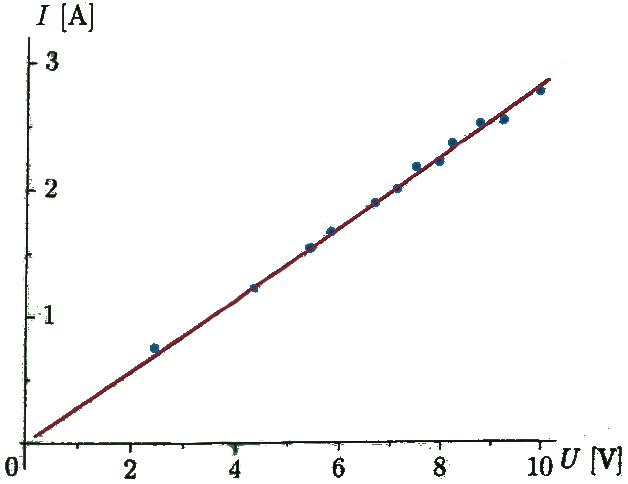
\includegraphics[width=0.8\linewidth]{mai_fig052.png}
  \captionof{figure}{Ověření Ohmová zákona lineární regresí.
  \cite[s.~263]{Musilova2009MA1}
  \label{mai:fig052}}
  \par}
  Pro odpor vychází \(R\doteq\SI{3.52}{\ohm}\). Součet čtverců odchylek přímky se směrnicí \(i/R
  = (1/\num{3.52})\Omega^{-1}\) od souboru bodů grafu je
  \begin{equation*}
    D(R) = \sum_{i=1}^{n}(U_i - R\cdot I_i)^2 \doteq\num{0.01},
  \end{equation*}
  \(\sigma(R) = \sqrt{D(R)/(n-1)}\doteq\sqrt{(\num{0.11}/11)}\doteq\num{0.03}\).  Graf přímky \(U
  = R\cdot I = \num{3.52}\cdot I\) proložené body je na obrázku \ref{mai:fig052}.
\end{mathexam}
      %---------------------------------------------------------------
      
      Popsaný způsob nalezení hodnoty elektrického odporu vodiče se nazývá\textbf{ metodou 
      nejmenších čtverců} (minimalizuje součet čtverců odchylek prokládané závislosti od souboru 
      naměřených bodů), v případě použití lineárního modelu, jako tomu bylo u Ohmová zákona, pak 
      jde o \textbf{lineární regresi}
      
      Obdobně se postupuje, je-li některá z měřených veličin lineární funkcí veličin jiných s 
      neznámými koeficienty lineární kombinace. Nechť
      \begin{equation*}
        Z = f(X_1, X_2, \ldots, X_K) = A_1X_1 + A_2X_2 + \cdots + A_KX_K.
      \end{equation*}
      Předpokládejme, že veličiny \(X_1, X_2, \ldots, X_K\) a \(Z\) měříme \(n\)-krát a naměříme 
      hodnoty
      \begin{equation*}
        X_j = \lbrace x_{j1}, \ldots x_{jn} \rbrace, \qquad 1 \leq j \leq K, \qquad 
        Z = \lbrace z_{1}, \ldots z_{n} \rbrace
      \end{equation*}
      Součet čtverců odchylek teoretické závislosti od naměřených bodů je
      \begin{equation*}
        D(Z) = \sum_{i=1}^{n}\left(z_i - \sum_{j=1}^{K}A_jx_{ji}\right)^2.
      \end{equation*}
      Nutnou podmínkou pro minimum tohoto výrazu jakožto funkce proměnných \(A_x, A_2, \ldots, A_K\)
      je platnost souboru rovnic
      \begin{equation*}
        \pder{D(Z)}{A_p} = 0 \Rightarrow 
        \sum_{i=1}^{n}2\left(z_i - \sum_{j=1}^{K}A_jx_{ji}\right)\cdot x_{pi} = 0
      \end{equation*}
      pro \(1 \leq i \leq n, 1 \leq j \leq K\). Tyto podmínky představují nehomogenní soustavu 
      \(K\) rovnic pro \(K\) neznámých \(( A_1, A_2, \ldots, A_K)\). Rozšířená matice soustavy je
      \begin{equation*}
        \overline{B} = (A|B) = 
          \left(
            \begin{array}{cccc|c}
              \sum_{i=1}^{n}x_{1i}x_{1i} & \sum_{i=1}^{n}x_{1i}x_{2i} & \cdots & 
              \sum_{i=1}^{n}x_{1i}x_{Ki} & \sum_{i=1}^{n}z_{i}x_{1i}                    \\
              \sum_{i=1}^{n}x_{1i}x_{1i} & \sum_{i=1}^{n}x_{2i}x_{2i} & \cdots & 
              \sum_{i=1}^{n}x_{2i}x_{Ki} & \sum_{i=1}^{n}z_{i}x_{2i}                    \\
                        \cdots           & \cdots & \cdots & \cdots   & \cdots          \\
              \sum_{i=1}^{n}x_{Ki}x_{1i} & \sum_{i=1}^{n}x_{Ki}x_{2i} & \cdots & 
              \sum_{i=1}^{n}x_{Ki}x_{Ki} & \sum_{i=1}^{n}z_{i}x_{Ki}                    \\
            \end{array}
          \right),
      \end{equation*}
      \begin{equation*}
        \sigma(z) = \sqrt{\dfrac{D(z)}{n - K}}.
      \end{equation*}
      V dalších kapitolách věnovaných lineární algebře se k tomuto problému znovu vrátíme a 
      ukážeme, že jej lze elegantně řešit také jako úlohu algebraickou, konkrétně úlohu o 
      ortogonální projekci vektorů na podprostory.
      
%} %tikzset
%---------------------------------------------------------------------------------------------------
\printbibliography[heading=subbibliography]
\addcontentsline{toc}{section}{Seznam literatury}
%  % !TeX spellcheck = cs_CZ
%{\tikzset{external/prefix={tikz/MAI/}}
% \tikzset{external/figure name/.add={ch07_}{}}
%---------------------------------------------------------------------------------------------------
% file: chap_Int_rfce_1var.tex
%---------------------------------------------------------------------------------------------------
%===================================================================================================
% ------------------------------------------- Definite Integral -----------------------------------
\chapter{Určitý integrál}
\minitoc

\section{Motivace} 

  \begin{figure}
    \centering
    \animategraphics[controls,autoplay,loop]{2}{mai_fig022}{}{}
    \caption{text
             (\cite[s.~10000]{Feynman01})}
  \end{figure}

  \begin{figure}[ht!]  %\ref{mai:fig031}
    \centering
    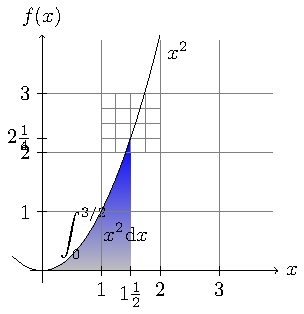
\includegraphics[width=0.7\linewidth]{mai_fig031.pdf}
    \caption{
            (\cite[s.~10000]{Feynman01})}
    \label{mai:fig031}
  \end{figure}

  \subsection{Výpočet integrálu}
      \begin{example}
        Spočítejme integrál $\displaystyle \int_1^{ln5}{(x+1)e^xdx}$  metodou per partes: 
        \begin{align*}
          \int{(x+1)e^xdx} &= \int{e^xdx}+\int{x\cdot e^xdx}
                            = e^x + (x-1)e^x = xe^x               \\
          \int_1^{ln5}{(x+1)e^xdx} &= [xe^x]_1^{ln5} = 5ln5-e     \\
        \end{align*}
        kde integrál
        \begin{equation*}
            \int{xe^xdx}=
              \left[\begin{array}{cc}
                u=x   & dv=e^x \\
                du=dx & v=e^x
              \end{array}\right]=
              xe^x-\int{e^xdx} = xe^x - e^x+C
        \end{equation*}
      \end{example}

\section{Vlastnosti určitého integrálu}
  V této kapitole mluvíme o spojitých funkcích $\Rightarrow$ příslušné integrály tedy vždy
  existují. Čerpáno z knih:
  \cite{Knichal}.

  \begin{lemma}
    \textbf{První věta o střední hodnotě integrálního počtu}: Je-li funkce $f(x)$ spojitá v
    intervalu $\langle a, b\rangle$, existuje alespoň jeden takový bod $c\in(a, b)$, že platí

    \begin{equation}\label{MA:eq_av1}
      \int_a^b f(x)dx = (b-a)f(c).
    \end{equation}
  \end{lemma}

  \begin{proof} Použitím Lagrangeovy věty napsané pro funkci $F(x)$, primitivní na intervalu
    $\langle a, b\rangle$ k dané funkci $f(x)$. Podmínky věty jsou zřejmě splněny: $F(x)$ je
    spojitá na intervalu $\langle a, b\rangle$ a má všude derivaci $F'(x)= f(x)$. Tedy existuje
    alespoň jeden bod $c\in(a, b)$,
    
    \begin{figure}[ht!]  %\ref{mai:fig029}
      \centering
      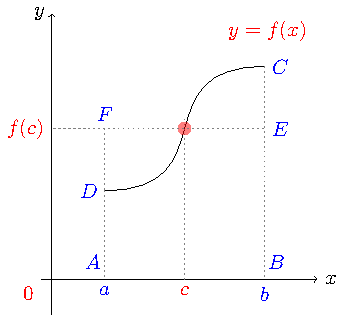
\includegraphics[width=0.7\linewidth]{mai_fig029.pdf}
      \caption{Vztah mezi silou tření a kolmou silou při smýkání
              (\cite[s.~173]{Feynman01})}
      \label{mai:fig029}
    \end{figure}

     že $$F(b)-F(a) = (b-a)F'(c),$$ čímž je věta dokázána, neboť $F(b)-F(a) = \int_a^bf(x)dx$ a
     $F'(c) = f(c)$. Funkční hodnotu $f(c)$, danou podle (\ref{MA:eq_av1}) rovnicí  
     \begin{equation}\label{MA:eq_av2}
        f(c) = \frac{1}{b-a}\int_a^b f(x)dx
     \end{equation}
     nazýváme \texttt{střední hodnotou}.
  \end{proof}

  Pro spojitou nezápornou funkci $f(x)$, lze větu o střední hodnotě jednoduše geometricky
  interpretovat dle (obr.\ref{mai:fig029}). Levá strana (\ref{MA:eq_av1}) určuje obsah
  křivočarého lichoběžníka $ABCD$, pravá strana obsah obdélníka $ABEF$. Podle této věty nabývá
  funkce $f(x)$ aspoň v jednom bodě intervalu $(a, b)$ takové hodnoty $f(c)$, že uvažovaný
  křivočarý lichoběžník má stejný obsah jako obdélník o základně $b-a$ a výšce $f(c)$ (str. 155
  knihy \cite{Knichal}).

      %---------------------------------------------------------------
      % !TeX spellcheck = cs_CZ
\begin{mdframed}[style=mdexam]
  \begin{example}\label{MAI:exam032}
    Určete střední hodnotu $i_s$ střídavého proudu $$i(t) = I_0\sin\omega t$$ v časovém intervalu
    $\langle 0, \frac{T}{2}\rangle$ (v průběhu jedné poloviny periody). $I_0$ je maximální hodnota
    proudu (obr. \ref{MAI:exam032}), perioda $T$ je dána vztahem $T = \frac{2\pi}{\omega}$
    
    {\centering
    \captionsetup{type=figure}
    \luafigure[1]{mai_fig030.pdf}
    \captionof{figure}{K příkladu \ref{MAI:exam032}
    \cite[s.~119]{Brabec1989}
    \label{mai:fig030}}
    \par}

      Podle \ref{MA:eq_av2} bude
      \begin{align*}
      i_s &=  \frac{2}{T}
              \int_0^{\frac{T}{2}}I_0\sin\omega t\dd{t} =
              \frac{2I_0}{T}\left[-\frac{\cos\omega t}{\omega}\right]_0^{\frac{T}{2}}        \\
          &=  \frac{2I_0}{T}\frac{1}{\omega}\left(-\cos\frac{\omega T}{2}+ \cos 0\right)     \\
          &=  \frac{2I_0}{2\pi}(-\cos\pi + \cos 0) = \frac{2}{\pi}I_0 \doteq 0,637 I_0.
    \end{align*}

    Tato hodnota se rovná intenzitě elektrického proudu, při kterém by vodičem v průběhu uvažované
    poloviny periody prošel stejný elektrický náboj jako při proudu střídavém.
  \end{example}
\end{mdframed}
















      %---------------------------------------------------------------

  \begin{example} Efektivní hodnota $i_{ef}$ střídavého proudu $$i(t) = I_0\sin\omega t$$ (viz
    předchozí příklad) je definována jako odmocnina ze střední hodnoty funkce $i^2(t)$ v průběhu
    jedné periody $T = \frac{2\pi}{\omega}$. Tedy
    \begin{align*}
      i_{ef}^2 &= \frac{1}{T}\int_0^T I_0^2\sin^2\omega t\dd{t} = 
                  \frac{1}{T}\int_0^T \frac{I_0^2}{2}(1- \cos2\omega t)\dd{t}           \\
               &= \frac{I_0^2}{2T}
                  \left[
                    t-\frac{\sin2\omega t}{2\omega}
                  \right]_0^T = \frac{I_0^2}{2}
    \end{align*}
    neboť $\sin2\omega T=\sin4\pi = 0.$ Odtud $$i_{ef} = \frac{I_0}{\sqrt{2}}.$$ Střídavý proud
    $i(t) = I_0\sin\omega t$ má na témže odporu stejný výkon jako stejnosměrný proud o intenzitě
    $i = 0,707I_0$.
  \end{example}
  Následující věta může být využita k odhadu některých integrálů
  \begin{lemma}
    \textbf{Druhá věta o střední hodnotě integrálního počtu}: Jsou-li funkce $f(x)$ a $g(x)$
    spojité v intervalu $\langle a, b \rangle$ a je-li funkce $g(x)$ v $\langle a, b \rangle$
    nezáporná a nerostoucí, existuje alespoň jeden bod $c\in\langle a, b \rangle$ tak, že platí
    \begin{equation}\label{MA_eq_av3}
        \int_a^b f(x)g(x) = g(a)\int_a^c f(x)dx.
    \end{equation}
  \end{lemma}
  Zcela obdobnou větu lze vyslovit pro případ, že $g(x)$ je v intervalu $\langle a, b \rangle$
  nezáporná a neklesající, tj. na pravé straně \ref{MA_eq_av3} je pak integrál $g(b)\int_c^b
  f(x)dx$

  \begin{example} Odhadněte hodnotu integrálu
    \begin{equation}\label{MA_eq_sinx_x}
        \int_{100\pi}^{1000\pi}\frac{\sin x}{x}dx
    \end{equation}
    Řešení: Funkce $f(x) = \sin x$ a $g(x) = \frac{1}{x}$ jsou v uvažovaném intervalu $\langle
    100\pi, 1000\pi \rangle$ spojité a funkce $g(x)$ je kladná a nerostoucí.
    \begin{equation*}
      \int_{100\pi}^{1000\pi}\frac{\sin x}{x}dx = 
      \frac{1}{100\pi}\int_{100\pi}^c\sin xdx =\frac{1}{100\pi}\left(\cos100\pi - \cos c\right)
    \end{equation*}
    kde $c$ je kladné číslo z intervalu $\langle 100\pi, 1000\pi \rangle$. Dále pro všechna
    $c\in\langle 100\pi, 1000\pi \rangle$ platí $0\leq1-\cos c\leq2$, takže
    \begin{equation*}
        0\leq\int_{100\pi}^{1000\pi}\frac{\sin x}{x}dx\leq \frac{1}{50\pi}.
    \end{equation*}
  \end{example}   

%} %tikzset
%---------------------------------------------------------------------------------------------------
\printbibliography[heading=subbibliography]
\addcontentsline{toc}{section}{Seznam literatury}
%  % !TeX spellcheck = cs_CZ
%{\tikzset{external/prefix={tikz/MAI/}}
% \tikzset{external/figure name/.add={ch04_}{}}
%---------------------------------------------------------------------------------------------------
% file: Theory_of_Derivates.tex
%---------------------------------------------------------------------------------------------------
\chapter{Derivace funkce}\label{mai:IchapIV}
\minitoc

%============== Kapitola: Derivace funkce ==========================================================
  \section{Základní věty diferenciálního počtu}
    \subsection{Věta o největší (nejmenší) hodnotě funkce}
      V tomto článku uvedeme významné věty, zvané souhrně věty o \emph{střední hodnotě 
      diferenciálního počtu}, a dále pak ukázky jejich užití v matematické analýze.  Avšak dříve 
      než budeme tyto věty formulovat, uvedeme jedno důležité tvrzení, které sice bude mít v 
      dalších úvahách tohoto článku pomocnou úlohu, ale v teorii extrémů má i samostatný význam. 
      \cite[s.~186]{Brabec1989} 
      \begin{lemma}\label{MA1:lem_diff02}
        Nechť funkce $f:A\rightarrow\realset$ nabývá na množině $A$ své největší (nejmenší) hodnoty 
        na vnitřním bodě $c$ množiny $A$. Máli funkce $f$ v bodě $c$ derivaci, potom $f'(c)=0$.  
      \end{lemma}
      \begin{proof}
        Nechť např. $f(c)$ je největší hodnota funkce $f$ na množině $A$, takže $f(x)\leq f(c)$ pro $\forall x\in A$. Potom pro $x\in A, x<c$, je 
        $$\frac{f(x)-f(c)}{x-c}\geq 0$$
        a tedy
        $$f'_{-}(c)=\lim_{x\rightarrow c^-}\frac{f(x)-f(c)}{x-c}\geq0$$ 
        Dále pro $x\in A, x>c$, je
        $$\frac{f(x)-f(c)}{x-c}\leq 0$$ 
        a proto
        $$f'_{+}(c)=\lim_{x\rightarrow c^+}\frac{f(x)-f(c)}{x-c}\leq0$$
        Platí tedy
        $$f'_{+}(c)\leq f'_{-}(c)\geq f'_{-}(c).$$ 
        Avšak $f'_{+}(c)=f'_{-}(c)= f'(c)$. Odtud plyne $f'(c)=0$. 
      \end{proof}
      
    \subsection{Věty o střední hodnotě}
      \begin{lemma}\label{MA1:lem_diff03}
        \textbf{Rolleova věta}\footnote{Michel Rolle [Mišel Rol] (1652-1719) Francouzský matematik} Nechť funkce $f$ má tyto vlastnosti:
          \begin{enumerate}
            \item je spojitá na uzavřeném intervalu $\langle a,b\rangle$;
            \item má derivaci (vlastní či nevlastní) na otevřeném intervalu $(a,b)$;
            \item platí $f(a)=f(b)$.
          \end{enumerate}
        Potom v otevřeném intervalu $(a,b)$ existuje aspoň jeden bod $\xi$ takový, že $f'(\xi)=0$.   
      \end{lemma}
      \begin{proof}
        Protože je funkce $f$ je na uzavřeném intervalu $\langle a,b\rangle$ spojitá, nabývá v 
        tomto intervalu své největší hodnoty $M$,své nejmenší hodnoty $m$. Přitom ovšem platí:
        \begin{equation}\label{MA1:eq_diff02}
          m\leq f(x) \leq M, \qquad x\in\langle a,b\rangle.
        \end{equation}
        Nyní mohou nastat dva případy: 
        \begin{enumerate}
          \item funkce $f$ nabývá $M$ i $m$ právě v krajních bodech intervalu $\langle a,b\rangle$. Podle předpokladu 3 věty \ref{MA1:lem_diff03}
                však potom platí $f(a)=f(b)=m=M$. Vzhledem ke vztahu \ref{MA1:eq_diff02} odtud plyne, že funkce $f$ je konstantní na intervalu
                $\langle a,b\rangle$ a tedy $f'(x)=0$ dokonce v každém bodě $x\in(a,b)$
          \item Funkce $f$ nabývá apsoň jedné z hodnot $M$, $m$ v některém vnitřním bodě $\xi$ intervalu $\langle a,b\rangle$. Potom podle 
          věty \ref{MA1:lem_diff02} je $f'(\xi)=0$.         
        \end{enumerate}        
      \end{proof}
      \begin{note}
        Rolleova věta sama zaručuje jen existenci aspoň jednoho bodu $\xi\in(a,b)$, ve kterém je fe 
        $f'(\xi)=0$. Neumožňuje však ani určení tohoto bodu (nebo bodů), ani stanovení jejich počtu 
      \end{note}
      
      \begin{note}
        Na obr. \ref{MAI:fig_027} je ilustrován geometrický význam Rolleovy věty. Graf funkce na 
        tomto obrázku má v bodech $\xi_1$, $\xi_2$, v nichž je $f'(\xi_1)=f'(\xi_2)=0$ tečny 
        rovnoběžné s osou $x$. 
        \begin{figure}[ht!] %\ref{MAI:fig_027}
          \centering
          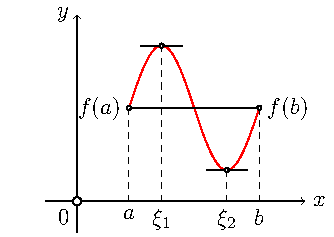
\includegraphics[width=0.7\linewidth]{mai_fig027.pdf}
          \caption{K výkladu Rolleovy věty}
          \label{MAI:fig_027}
        \end{figure}
      \end{note}
      
      Z Rolleovy věty plyne důležitá věta:
      
      \begin{lemma}\label{MA1:lem_diff04}
        (\textbf{Cauchyova věta}). Nechť funkce $f$ a $g$ mají tyto vlastnosti:
        \begin{enumerate}
          \item  Jsou spojité na uzavřeném intervalu $\langle a,b\rangle$,
          \item  v každém bodě $x\in(a,b)$ existuje derivace $f'(x)$ (vlastní či nevlastní) a vlastní derivace $g'(x)$,
          \item  $g'(x)\neq0$ na $(a,b)$
        \end{enumerate}
        Potom v otevřeném intervalu $(a,b)$ existuje aspoň jeden bod $\xi$, pro který platí
        \begin{equation}\label{MA1:eq_diff03}
          \frac{f(b)-f(a)}{g(b)-g(a)} = \frac{f'(\xi)}{g'(\xi)}.
        \end{equation} 
      \end{lemma} 
      
      \begin{proof}
        Poznamenejme především, že z předpokladu 3 $g'(x)\neq0$ pro $x\in(a,b)$ a z předpokladu 
        spojitosti funkce $g$ na uzavřeném intervalu $\langle a,b\rangle$ ihned vyplývá vztah 
        $g(b)- g(a)\neq 0$. Kdyby totiž bylo $g(b)=g(a)$, potom by podle \emph{Rolleovy věty} 
        \ref{MA1:lem_diff03} existoval aspoň jeden bod $\eta\in(a,b)$ takový že $g'(\eta)=0$. To 
        však by byl spor s předpokladem $g'(x)\neq0$ pro každý bod $x\in(a,b)$. Proto má smysl 
        podíl na levé straně rovnosti \ref{MA1:eq_diff03}
        
        K vlastnímu důkazu Cauchyovy věty zavedeme takovou pomocnou funkci $F$, aby splňovala podmínky Rolleovy věty. Definujme ji pro $x\in\langle a,b\rangle$ předpisem
        \begin{equation}\label{MA1:eq_diff04}
          F(x)=[f(b)-f(a)]\cdot[g(x)-g(a)]-[f(x)-f(a)]\cdot[g(b)-g(a)].
        \end{equation}
        Snadno ověříme, že tato funkce skutečně splňuje podmínky Rolleovy věty na intervalu $\langle a,b\rangle$:
        \begin{itemize}
          \item Je spojitá na intervalu $x\in\langle a,b\rangle$, což je důsledkem spojitosti  
                funkce $f$ a $g$ na intervalu $x\in\langle a,b\rangle$ ,
          \item má derivaci $F'$ na otevřeném intervalu $(a,b)$, což plyne z existence derivace  
                $f'$ a $g'$ funkce $f$ a $g$ na  intervalu $(a,b)$,
          \item $F(a)=F(b)=0$ 
        \end{itemize}
        Platí tedy i závěr Rolleovy věty pro funkci $F$, tj. na intervalu $(a,b)$ existuje aspoň 
        jeden bod $\xi$, pro který $F'(\xi)=0$. Zderivujeme-li funkci $F$, dostaneme (dosadíme-li 
        $x=\xi$): $$F'(\xi)=[f(b)-f(a)]g'(\xi)-f'(\xi)[g(b)-g(a)]=0$$ Odtud již plyne rovnost 
        \ref{MA1:eq_diff03}                  
      \end{proof}
      
      Významným zvláštním případem Cauchyovy věty je další věta, která se častěji používá.
      
      \begin{lemma}\label{MA1:lem_diff05}
        (\textbf{Lagrangeova věta})\footnote{Joseph Louis Lagrange [lagránž] (1736-1813), francouzský matematik}. Nechť funkce má tyto vlastnosti:
        \begin{itemize}
          \item Je spojitá na intervalu $\langle a,b\rangle$,
          \item má derivaci (vlastní či nevlastní) na otevřeném intervalu $(a,b)$. 
        \end{itemize} 
        Potom existuje v otevřeném intervalu $(a,b)$ aspoň jeden bod $\xi$, pro který platí 
        \begin{equation}\label{MA1:eq_diff05}
           \frac{f(b) - f(a)}{b - a} = f'(\xi),  
        \end{equation}  
        či-li
        \begin{equation}\label{MA1:eq_diff06}
           f(b) - f(a) = f'(\xi)(b-a),  
        \end{equation}           
      \end{lemma}
      
      \begin{proof}
        Tvrzení této věty je důsledkem tvrzení \emph{Cauchyovy věty}, a to pro případ $g(x)=x$. 
        Protože $g'(x)=1$ dokonce všude, jsou splněny všechny tři podmínky Cauchyovy věty. Proto 
        platí i závěr této věty, z něhož pro náš případ již plyne vzorec \ref{MA1:eq_diff05} a tedy 
        i vzorec \ref{MA1:eq_diff06}.  
      \end{proof}
      
      \begin{note}
        Podobně jako je Lagrangeova věta zvláštním případem věty Cauchyovy, je Rolleova věta zvláštním případem Lagrangeovy věty, a to přo případ, že $f(a)=f(b)$.
      \end{note}
      
      \begin{note}
        Lagrangeova věta se často nazývá \emph{větou o přírůstku funkce}, protože vzorcem \ref{MA1:eq_diff06} se vyjadřuje \emph{přírůstek funkce}, tj rozdíl $f(b)-f(a)$. 
        Všechny tři uvedené věty, tj. věta Rolleova, Cauchyova a Lagrangeova, se v literatuře nazývá souhrně \textbf{věty o střední hodnotě diferenciálního počtu}.
      \end{note}
      
      \begin{note}
        Na obr. ** je ilustrován geometrický význam Lagrangeovy věty. Podíl na levé straně rovnosti 
        \ref{MA1:eq_diff05}, tj. číslo $\frac{f(b) - f(a)}{b - a}$ je směrnice sečny $s$, spojující 
        body $A$, $B$ grafu funkce  $f$, které odpovídají krajním bodům intervalu $\langle 
        a,b\rangle$. Podle tvrzení Lagrangeovy věty existuje v otevřeném intervalu $(a,b)$ aspoň 
        jeden bod $\xi$ tak, že tečna grafu funkce $f$ v příslušném jeho bodě je rovnoběžná s 
        přímkou $s$.  
      \end{note}
      
      \begin{note}
        Z Lagrangeovy věty vyplývá toto tvrzení: Nechť funkce $f$ vyhovuje na intervalu $\langle a,b\rangle$ podmínkám Lagrangeovy věty a $x_1$, $x_2$ jsou dva libovolné různé body
        intervalu $\langle a,b\rangle$. Potom v otevřeném intervalu s krajnímy body $x_1$, $x_2$ existuje aspoň jeden bod $\xi$, pro který platí Lagrangeův vzorec:   
        \begin{align}
          f(x_2) - f(x_1)                  &= f'(\xi)(x_2-x_1) \label{MA1:eq_diff07} \\ 
          \frac{f(x_2) - f(x_1)}{x_2-x_1}  &= f'(\xi)          \label{MA1:eq_diff08}      
        \end{align}
        Potom bod $\xi$ lze vyjádřit takto:
        \begin{equation}\label{MA1:eq_diff09}  
          \xi = x_1 + \vartheta(x_2-x_1), \qquad \text{kde }\vartheta\in(0,1). 
        \end{equation}
        Označíme-li $x_2-x_1=h$, můžeme vzorec \ref{MA1:eq_diff07} napsat ve tvaru
        \begin{equation}
          f(x_1+h) - f(x_1)= f'(x_1 + \vartheta h)h, \qquad \text{kde }\vartheta\in(0,1). 
        \end{equation} 
      \end{note}       
          
    \subsection{Některé důsledky Lagrangeovy věty}
      Lagrangeova věta, má některé významné důsledky, které nyní uvedeme \cite[s.~189]{Brabec1989}:
      \begin{lemma}\label{MA1:lem_diff06} 
        Nechť funkce $f$ vyhovuje podmínkám Lagrangeovy věty a navíc nechť $f'(x)=0$ pro všechna 
        $x\in(a,b)$. Potom funkce $f$ je prostá na intervalu $\langle a,b \rangle$. 
      \end{lemma}
      \begin{proof}
        Necť $x_1, x_2$ jsou libovolné dva různé body intervalu $\langle a,b \rangle$. Potom podle 
        Lagrangeova vzorce \ref{MA1:eq_diff04} platí 
        \begin{equation}
          f(x_2) - f(x_1) = f'(\xi)(x_2-x_1) \neq0
        \end{equation}
        neboť $f'(\xi)\neq 0$ dle předpokladu.
      \end{proof}
      
      \begin{lemma}\label{MA1:lem_diff01}
        Funkce $f$ je konstantní na intervalu $(a,b)$, právě když má na tomto intervalu derivaci a platí $f'(x) = 0$ pro všechna $x\in(a,b)$. 
      \end{lemma}
      \begin{proof} Tedy
        \begin{itemize}
          \item Je-li funkce $f$ konstantní na intervalu $(a,b)$, pak je $f'(x) = 0$ pro všechna  
                $x\in(a,b)$, jak již víme.
          \item Nechť $f'(x) = 0$ pro všechna $x\in(a,b)$. Dokažme, že pro každé dva body $x_1, 
                x_2  \in(a,b)$, $x_1\neq x_2$, platí $f(x_1) = f(x_2)$. Z existence
                derivace vyplývá spojitost funkce a jsou tedy splněny podmínky Lagrangeovy věty na 
                každém intervalu $\langle x_1, x_2\rangle\subset(a,b)$. Podle vzorce 
                \ref{MA1:eq_diff04} tedy platí $f(x_2)-f(x_1)f'(\xi)(x_2-x_1)$, $\xi\in(x_1,x_2)$. 
                Protože podle předpokladu je $f'(x)=0$ pro $\forall x\in(a,b)$, platí $f(x_1) 
                -f(x_2)=0$, tj. $f(x_1)=f(x_2)$  
        \end{itemize}
      \end{proof}
      
%} % tikzset
%---------------------------------------------------------------------------------------------------
\printbibliography[heading=subbibliography]
\addcontentsline{toc}{section}{Seznam literatury}
%  % !TeX spellcheck = cs_CZ
%{\tikzset{external/prefix={tikz/MAI/}}
% \tikzset{external/figure name/.add={ch05_}{}}
%---------------------------------------------------------------------------------------------------
% file: Differential_Calculus_applications.tex
%---------------------------------------------------------------------------------------------------
\chapter{Aplikace diferenciálního počtu}\label{chap:Apl_dif_poc}
\minitoc

%================Kapitola: Aplikace diferenciálního počtu =========================================
Diferenciální počet má rozsáhlou oblast užití. V této kapitole ukážeme použití výsledků předchozích 
kapitol k vyšetřování průběhu funkce a vlastnosti rovinných křivek. 
  \section{Průběh funkce}
    Pomocí derivace můžeme studovat vlastnosti funkce, které usnadní vyšetřování jejího průběhu.  
    \subsection{Monotonie funkcí}
      Jednou z důležitých vlastností funkce je její \textquotedblleft monotonie\textquotedblright, 
      kterou jsme definovali již v odst. \ref{MA1:subsec_vlastnosti_funkce} kap. 
      \ref{mai:IchapLimit}. Proto je při vyšetřování průběhu funkce důležité určit množiny (často 
      jsou to intervaly), na nichž je funkce monotónní, jinak řečeno, najít \textquotedblleft 
      intervaly monotonie funkce\textquotedblright (viz \cite[s.~208]{Brabec1989}). 
    \begin{enumerate}
      \item Zjistíme \textbf{definiční obor funkce}, vyjádříme jej v intervalech a z nich poznáme,  
            kde je funkce \textbf{spojitá}. Funkce je spojitá v $(a,b)$ pro každý bod tohoto 
            intervalu, když$|f(x)-f(c)|<\varepsilon$, kde $\varepsilon>0$ je libovolně zvolené 
            číslo, a pro všechna $x$ z okolí bodu $c$ je $|x-c|<\delta$, kde $\delta>0$ je na 
            $\varepsilon$ nezávislé.
      \item Určíme, je-li funkce \textbf{lichá} $f(-x)=-f(x)$ nebo \textbf{sudá} $f(-x)=f(x)$.   
            Je-li funkce lichá, je souměrná podle středu souměrnosti (obyčejně to bývá počátek 
            souřadnic $xy$), je-li sudá, je souměrná podle osy $y$.
      \item Určíme \emph{průsečíky křivky s osami pravoúhlých souřadnic}. Body, ve kte\-rých 
            křivka  protíná osu $x$ spolu s body, ve kte\-rých není křivka spojitá, rozlišují 
            intervaly, v nichž je graf křivky nad osou $x$ od intervalů, ve kterých je graf křivky 
            pod osou $x$.
      \item V krajních bodech definičních intervalů, ve kterých je funkce spojitá, stano\-víme 
      \emph{limity funkce} a dále $$\lim_{x \to \pm \infty}f(x).$$
      \item Vypočítáme $f'(x)$ a $f''(x)$, abychom zjistily, kde je funkce \emph{rostoucí}     
            $f'(x)>0$, \emph{klesající} $f'(x)<0$ a kde jsou \emph{lokální extrémy}. Dostaneme-li 
            dosazením kořenů rovnice $f'(x)=0$ do $f''(x)$ hodnotu $f''(x)>0$, má funkce lokální 
            minimum, při $f''(x)<0$ má funkce lokální maximum. V intervalech, kde $f''(x)>0$, je 
            křivka \textbf{konvexní (vypuklá)}, kde $f''(x)<0$, je křivka \textbf{konkávní 
            (vydutá)}. Body, v nichž $f''(x)$ mění znaménko, jsou \textbf{inflexní body}. Najdeme 
            je tak, že stanovíme hodnoty $x$, pro které je $f''(x)=0$ nebo neexistuje. Číslo $c$ je 
            inflexní bod, když existuje takové okolí bodu $c$, že pro $x>c$ je oblouk křivky 
            konvexní a pro $x<c$ konkávní. Je nutné si uvědomit, že když má $f'(x)$ konečnou 
            derivaci, je inflexní bod $c$ taky nulovým bodem druhé derivace čili kořenem rovnice 
            $f''(x)=0$. Obrácená věta neplatí, tj. z $f''(x)=0$ nevyplývá, že v bodě $c$ má $f'(x)$ 
            extrém a že bod $c$ je inflexním bodem.
      \item \textbf{Asymptota} je tečna křivky $f(x)$, jejíž bod dotyku je v nekonečnu. Platí-li  
            $$\lim_{x \to a}f(x) =  \pm\infty,$$ je přímka $x=a$ její asymptotou. Jinak asymptoty 
            mají rovnici $y=kx+q$, kde $x$ a $y$ jsou souřadnice bodů na asymptotách. Existují-li 
            konečné limity $$\lim_{x \to \pm\infty}\frac{f(x)}{x}=k$$  a $$\lim_{x \to 
            \pm\infty}[f(x)-kx] =q$$ pak je asymptotou přímka $y=kx+q$. Můžeme-li rovnici křivky 
            rozložit (tj. rozložit její pravou stranu, oby\-čejně dělením čitatele jmenovatelem, 
            má-li tvar zlomku) na dvě části, z nichž jedna má tvar $kx+q$ a druhá zbytek 
            $\varphi(x)$, tj. $f(x)=kx+q+\varphi(x)$ a $\varphi(x)_{x\rightarrow 
            \pm\infty}\rightarrow 0$, je přímka $y=kx+q$ asymptotou.
      \item Zpřesnění grafu křivky provedeme sestavením tabulky souřadnic dalších bodů křivky,  
            tj. ke zvoleným hodnotám $x$ (z definičního oboru funkce) vypočítáme hodnoty $y$. Do 
            dalších řádků tabulky zapíšeme hodnoty  $f'(x)$ a $f''(x)$, ve kterých intervalech je 
            funkce \emph{rostoucí}, ve kterých \emph{klesá}, kde je \emph{vypuklá}, kde je 
            \emph{dutá}, kde jsou \emph{lokální extrémy}, \emph{inflexní body} apod., 
            případně sestavíme dílčí tabulky pro jednotlivé \emph{charakteristické vlastnosti} vyšetřované funkce.
    \end{enumerate}
    %-------------------- EXAM001 --------------------------------------
    % !TeX spellcheck = cs_CZ
\begin{mathexam}{Vyšetřete průběh funkce \(f(x):y=\frac{1+x^2}{1-x^2}\)}{exam003}
  \begin{enumerate}[noitemsep]
    \item Definiční obor $D_f=\realset-\{±1\}=(-\infty,-1)\cup(-1,1)\cup(1,+\infty)$
    \item Funkce je sudá $$f(-x)=f(x): \frac{1+x^2}{1-x^2}=\frac{1+(-x)^2}{1-(-x)^2}.$$ Funkce není
        periodická.
    \item Stanovíme funkční hodnoty v krajních bodech definičního obor $1, -1$ a v nevlastních
        bodech $-\infty,+\infty$.Protože je funkce \textbf{sudá}, omezíme se jen na vyšetřování
        nezáporné části. Nejprve vlastnosti funkce v okolí bodu $1$. Ten nepatří do $D_f$ a proto
        určíme limity funkce v pravém a levém okolí tohoto bodu. $$\lim_{x\to
        1_{-}}=\frac{1+x^2}{1-x^2}.$$ Pro výpočet limity použijeme substituci $y=1-x^2$: 
        $$\lim_{y\to0+}\frac{2-y}{y}=+\infty$$ \footnote{$\lim_{x\to0_+}\frac{1}{x}=\infty$} proto
        
        $$\lim_{x\to1_{-}}\frac{1+x^2}{1-x^2}=+\infty.$$ Obdobně dojdeme k
        $$\lim_{x\to1_+}\frac{1+x^2}{1-x^2}=-\infty.$$ A konečně v nevlastních bodech $±\infty$ je
        limita $$\lim_{x\to±\infty}\frac{1+x^2}{1-x^2} = \lim_{x\to\pm\infty}\frac{1}{1-x^2} +
        \lim_{x\to\pm\infty}\frac{x^2}{1-x^2}=0-1=-1.$$ Výpočtem limit jsme zároveň určili dva
        absolutní (globální) extrémy a jeden lokální:
        \begin{itemize}
          \item v intervalu $(-1,1)$ má funkce maximum $\infty$ a minimum $1$,
          \item v intervalech $(-1,1)\cup(1,+\infty)$ má funkce minimum $-\infty$ a maximum $-1$.
        \end{itemize}
    \item Nyní vyšetříme zda, případně kolik a jaké, má funkce $f(x)$ průsečíky s osami souřadnic. S
        osou $x$ nemá funkce žádné průsečíky, protože pro $y=0$ není definována
        $H_f=\realset-\{-1,1\rangle$. Pro $x=0$ je $y=\frac{1+0^2}{1-0^2}=1$, proto má $f(x)$ právě
        jeden průsečík s osou $y$ a to $[0,1]$.
    \item Zatím jsme zjistili, že naše funkce není definována v bodech $1$ a $-1$ a proto není
        spojitá v  $\realset$. Nevíme však, jaký je její průběh v jednotlivých intervalech
        definičního oboru.  Abychom získali názornější představu o průběhu funkce, zjistíme má-li
        derivaci.
        \begin{align*}
          y' &= \frac{(1+x^2)'(1-x^2 )-(1+x^2)(1-x^2 )'}{(1-x^2)^2} \\
          y' &= \frac{2x(1-x^2 )-(1+x^2 )(-2x)}{(1-x^2 )^2}         \\
          y' &= \frac{4x}{(1-x^2 )^2}
        \end{align*}
        Protože má vlastní derivaci\footnote{$f(x)$ je spojitá v intervalech $(-\infty,-1),
        (-1,1),(1,\infty)$  věta s spojité funkci}, můžeme určit její vlastnosti v intervalech
        $\langle0,1)$ a $(1,\infty)$. V těchto intervalech je $y'>0$ a proto jde o funkci ryze
        monotónní, rostoucí \footnote{Plyne z věty o postačujících podmínkách ryzí monotónnosti
        funkce na intervalu} v daných intervalech \footnote{V intervalech
        $(-\infty,-1),(-1,0\rangle$ je funkce klesající.}. Výpočtem zjistíme druhou derivaci funkce.
        Ta nám pomůže určit další extrém v intervalu $\langle0,1)$ a zároveň vyšetřit
        \textbf{konkávnost} a \textbf{konvexnost}.
        \begin{align*}
          y'' &= \frac{(4x)' (1-x^2 )^2-(4x)(1-2x^2+x^4 )'}{(1-x^2 )^4}  \\
          y'' &= \frac{4(1-2x^2+x^4 )-4x(-4x+4x^3 )}{(1-x^2 )^4}         \\
          y'' &= \frac{4(1-x^2 )(3x^2+1)}{(1-x^2 )^4}                    \\
          y'' &= \frac{4(3x^2+1)}{(1-x^2 )^3}
        \end{align*}
        Abychom mohli určit lokální extrém funkce $f(x)$ v intervalu $\langle0,1)$, pomocí druhé
        derivace, musíme najít kořeny rovnice $f' (x)=0$. V našem případě
        $$y'=\frac{4x}{(1-x^2)^2}\Rightarrow\frac{4x}{(1-x^2)^2}=0\rightarrow x_0=0,$$ tento kořen
        \footnote{stacionární bod}  pak dosadíme do druhé derivace, tj. 
        $$y''(0)=\frac{4(3\cdot0^2+1)}{(1-0^2 )^3}=4,$$ protože je $f''(x)>0$, má v bodě $x_0$
        lokální minimum. Můžeme rovněž konstatovat, že funkce nemá inflexní body \footnote{Pro
        existenci inflexního bodu je nutné splnění jedné z podmínek a to buď $f''(x_0)=0$, nebo
        $f''(x_0)$ neexistuje.}. Konkávnost a konvexnost funkce v intervalech $\langle0,1)$ a
        $(1,\infty)$ vyšetříme pomocí vlastností druhé derivace funkce. Tedy
        \begin{itemize}
          \item $\langle0,1): y''=\frac{4(3x^2+1)}{(1-x^2 )^3} >0 \Rightarrow$ funkce je v tomto
                intervalu \textbf{konvexní},
          \item $(1,\infty): y''=\frac{4(3x^2+1)}{(1-x^2 )^3} <0 \Rightarrow$ funkce je v tomto
                intervalu \textbf{konkáv\-ní}.
        \end{itemize}
    \item Z předchozích výpočtů plyne, že křivka má asymptoty $y=-1,x=\pm1$.
  \end{enumerate}
  {\centering \captionsetup{type=figure}          % %\ref{MAI:fig_028}
    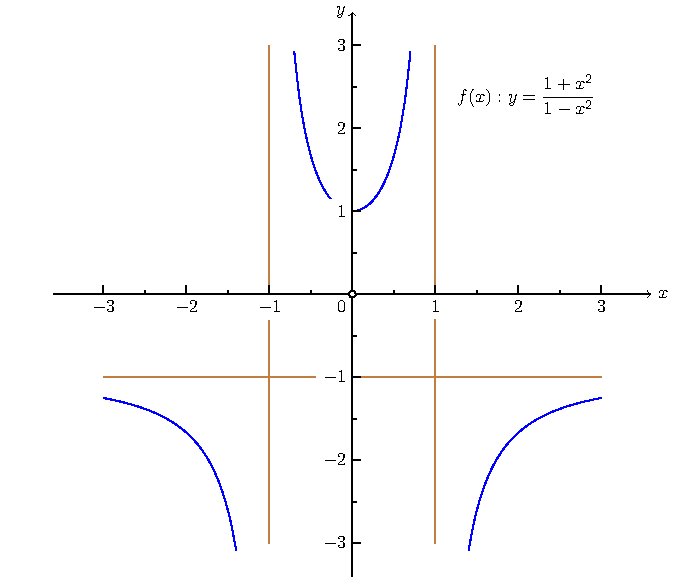
\includegraphics[width=1\linewidth]{mai_fig028.pdf}
    \captionof{figure}{Graf funkce $f(x):y=\dfrac{1+x^2}{1-x^2}$}
    \label{MAI:fig_028}
  \par}
\end{mathexam}  
    %-------------------------------------------------------------------

%} %tikzset
%---------------------------------------------------------------------------------------------------
\printbibliography[heading=subbibliography]
\addcontentsline{toc}{section}{Seznam literatury} 
%  % !TeX spellcheck = cs_CZ
%{\tikzset{external/prefix={tikz/MAI/}}
% \tikzset{external/figure name/.add={ch06_}{}}
%---------------------------------------------------------------------------------------------------
% file: chap_PrimitiveFce.tex
%---------------------------------------------------------------------------------------------------
%============================ Primitivní funkce ====================================================
\chapter{Primitivní funkce}
\minitoc

  %----------------------------Neurčitý integrál----------------------------------------------------
  \section{Motivace}
    Problém \emph{neurčitého integrálu}, neboli \textbf{primitivní funkce}, lze vyložit velmi 
    jednoduše: Máme podezření, že zadaná funkce \(f(x)\) vznikla derivováním jisté, zatím neznámé, 
    funkce \(F(x)\). Dokážeme ji najít? 
  
    K danému problému můžeme přistupovat také fyzikálně: Zavedením pojmu derivace funkce jsme 
    motivovali důležitým požadavkem definovat okamžitou rychlost pohybu bodu po přímce. Existuje 
    přirozeně i požadavek opačný, tj. nalézt zákon dráhy pohybu bodu po přímce, je-li dána jeho 
    okamžitá rychlost jako funkce času \cite[s.~253]{Brabec1989}. Vše si ukážeme na následujícím 
    příkladu:  
   
    \begin{example}
      Je dána okamžitá rychlost $v$ pohybu bodu po přímce (ose) $x$ rovnicí $v(t) = 2t + 1$, 
      $t\in\langle -\infty,+\infty \rangle$. Najděte zákon dráhy pohybu, je-li známo, že v čase $t 
      = 0$ měl bod polohu $x = x_0$.
      \newline
      \textbf{řešení:}\newline
      Označíme-li $x(t)$ polohu bodu v okamžiku $t$, pak $v(t) = \frac{dx}{dt}$. Hledáme tedy 
      funkci $x = x(t)$, pro níž platí 
      \begin{align}
        \frac{dx}{dt} &= 2t + 1 \qquad x(0) = x_0.  \nonumber \\ 
        \shortintertext{Je ihned patrné, že první podmínce vyhovuje nekonečně mnoho funkcí}
        x(t)          &= t^2 + t + C,           \label{MA:int_ex_09}    \\ 
        \shortintertext{ kde $C$ je libovolná konstanta. Funkce, která splňuje i druhou podmínku 
          (říkáme ji též počáteční podmínka), najdeme z rovnice \ref{MA:int_ex_09} dosazením dané podmínky 
          $t = 0,\ x = x_0$. Dostaneme $x_0 = C$. Dosazením do \ref{MA:int_ex_09} za $C$ plyne hledaný 
          zákon dráhy}
        x(t)          &= t^2+t+x_0.                 \nonumber 
        \shortintertext{Jednoduchou zkouškou se přesvědčíme, že tato funkce splňuje obě dané podmínky a 
          zároveň vidíme, že hledaná primitivní funkce daných vlastností je jediná.}  \nonumber
      \end{align}
    \end{example} 
    Každé takové funkci, jejíž derivací je daná funkce, budeme říkat \emph{primitivní funkce} k 
    dané funkci. Na uvedeném příkladě je patrné, že k dané funkci může existovat nekonečně mnoho 
    primitivních funkcí. Množinu všech primitivních funkcí se často nazývá \textbf{neurčitým 
    integrálem}. Po tomto názorném uvedení do problému přejděme k přesné formulaci základních pojmů.
    
    \begin{definition} 
      Funkce $F: J\rightarrow \realset$, kde $J\subset \realset$ je interval, se nazývá primitivní 
      funkce k funkci \(f\) na intervalu \(J\) právě když, pro všechna $x\in J$ je $F'(x) = f(x)$ 
      (v krajních bodech intervalu \(J\), pokud k němu patří, jde o derivace jednostranné).
    \end{definition}
    
    \begin{example} 
      K funkci $\sin x$ je primitivní funkcí na libovolném intervalu $J\subset(-\infty,+\infty)$ 
      funkce $-\cos x$, protože $(-\cos x)' = \sin x$. Ale též funkce $3-\cos x$ je primitivní 
      funkcí k funkci $\sin x$, protože $(3 - \cos x)' = \sin x$ pro všechna $x\in(-\infty, 
      \infty)$.
    \end{example}
    
    Je vidět, že rozdíl dvou primitivních funkcí k téže funkci je konstanta. To není náhoda, jak 
    potvrzuje následující věta:
    
    \begin{lemma}
      \begin{enumerate}
        \item Je-li funkce $F$ primitivní funkcí k funkci \(f\) na intervalu \(J\) a \(c\) reálná  
              konstanta, pak i funkce $G = F + c$ je primitivní funkcí k funkci \(f\) na intervalu 
              \(J\).
        \item Jsou-li funkce $F$ a $G$ primitivní funkce k funkci \(f\) na intervalu \(J\), pak 
        funkce
              $F-G$ je na intervalu \(J\) konstantní.
      \end{enumerate} 
      \begin{proof}
        Tvrzení a) plyne z definice protože $G'(x) = [F(x) + c] = F'(x) = f(x)$ pro všechna $x\in
        J$. Tvrzení b) je důsledkem věty \ref{MA1:lem_diff01}.
      \end{proof}
    \end{lemma}
    Neurčitost vyplývá právě z toho, že primitivní funkce není dána jednoznačně, je určena až na 
    konstantu. Značíme
    \begin{equation*}
      \boxed{F(x) = \int f(x)\dx + C}
    \end{equation*}
        
    Jak ale primitivní funkce hledat? V jednoduchých příkladech poslouží tabulka derivací, již 
    čteme „zprava doleva“. (Je dobré si ji uložit do paměti.) Tabulka však pokryje jen velmi málo 
    případů, pouze elementární funkce. Je tedy třeba najít metody, jak při hledání primitivních 
    funkcí postupovat. Nejprve však uvedeme dvě základní pravidla pro primitivní funkce, která 
    plynou z pravidel pro derivování:
    \begin{align}
      \int[f(x)\pm g(x)]\dx &= \int[f(x)\pm g(x)]\dx + \int[f(x)\pm g(x)]\dx \label{MA1:eq_int10} \\
      \int cf(x)\dx         &= c \int f(x)\dx, \qquad \text{\(c\) je konstanta.} \label{MA1:eq_int11}
    \end{align}
  
  \section{Tabulka neurčitých integrálů}\label{MA:chap_tabINT}
    Pokud není nic uvedeno, platí vzorce pro všechna \(x\) a pro všechny hodnoty uvedených
    konstant. Místo platí pro \(x\) z intervalu \((-\infty,0),(0,+\infty)\) píšeme stručně
    \(x\neq0\) apod. Literatura: \cite[p.~396]{Rektorys1963}.
  
    \begin{flalign}
      & \int 0\dx = c                                        &         \label{MA:baseInt01}     \\
      & \int a\dx = ax+c                                     &         \label{MA:baseInt02}     \\
      & \int x^n\dx = \frac{x^{n+1}}{n+1}+c, \,              &         \label{MA:baseInt03}     \\
      & \qquad\text{kde}\begin{cases}
          \forall x\in\realset,\,n\in\naturalset, n>0,         \\
          \forall x\in\realset-\{0\},\,n\in\naturalset, n<-1,  \\
          \forall x>0,\,n\in\realset\,\,n\notin\naturalset
        \end{cases}                                          &         \nonumber               \\
      & \int\frac{1}{x}\dx = 
            \ln\abs{x}+c \hspace{1ex}\forall x\neq0          &         \label{MA:baseInt04}     \\
      & \int e^x \dx       = e^x+c                           &         \label{MA:baseInt05}     \\
      & \int\ln x\dx       = 
          x\ln x - x + c \hspace{1ex}\forall x>0             &         \label{MA:baseInt06}     \\
      & \int a^x \dx     =
          \frac{a^x}{\ln a}+c 
          \hspace{1ex}\forall a>0,\,a\neq1                   &         \label{MA:baseInt07}     \\
      & \int \sin x \dx  = -\cos x                           &         \label{MA:baseInt08}     \\
      & \int \cos x \dx  =  \sin x                           &         \label{MA:baseInt09}     \\
      & \int\frac{1}{\cos^2x}\dx =  \tan x+c 
           \hspace{1ex}\forall x\neq(2k+1)\pi,\,k\in\naturalset &      \label{MA:baseInt10}     \\ 
      & \int\frac{1}{\sin^2x}\dx     =  -\cotg x+c
         \hspace{1ex}\forall x\neq k\pi,\,k\in\naturalset    &         \label{MA:baseInt11}     \\
      & \int\frac{1}{\sqrt{1-x^2}}\dx =
          \begin{cases}
            +\arcsin x + c         \\
            -\arccos x + c
          \end{cases} 
          \forall x\in(-1,1)                                 &         \label{MA:baseInt12}     \\
      & \int\cosh\dx = \sinh x + c                           &         \label{MA:baseInt13}     \\
      & \int\sinh\dx = \cosh x + c                           &         \label{MA:baseInt14}     \\
      & \int\frac{1}{1+x^2}\dx = \arctan x + c               &         \label{MA:baseInt15}     \\
      & \int \frac{1}{\sqrt{x^2 + 1}}\dx =
          \begin{cases}
            \ln(x + \sqrt{x^2+1}) + c         \\
            \sinh^{-1}x + c 
          \end{cases}                                        &         \label{MA:baseInt16}     \\ 
      & \int \frac{1}{\sqrt{x^2 - 1}}\dx =
          \begin{cases}
            \ln(x + \sqrt{x^2-1}) + c         \\
            \cosh^{-1}x + c \hspace{4ex}x\in(1,+\infty) 
          \end{cases}                                        &         \label{MA:baseInt17}     \\
      & \int\frac{1}{\sqrt{x^2+a^2}}\dx 
        = \sinh^{-1} \frac{x}{a} = \ln (x+\sqrt{x^2+a^2})    &         \label{MA:baseInt18}     \\
      & \int \frac{1}{\sqrt{x^2-a^2}}\dx 
        = \cosh^{-1} \frac{x}{a} = \ln (x+\sqrt{x^2-a^2})    &         \label{MA:baseInt19}     \\
      & \int\frac{1}{\sqrt{x^2-1}}\dx 
        = \left\{ 
          \begin{array}{l l}
            \ln\abs{x+\sqrt{x^2-1}}+c      &  \abs{x}>1  \\
            \cosh^{-1}x+c                  &  \abs{x}<1
          \end{array} 
          \right.                                            &         \label{MA:baseInt20}     \\
      & \int\tan x \dx   = \ln |\sec x| + c                  &         \label{MA:baseInt21}     \\
      & \int\sec x \dx   = \ln |\sec x + \tan x| + c         &         \label{MA:baseInt22}     \\
      & \int\sec^2 x \dx = \tan x + c                        &         \label{MA:baseInt23}     \\
      & \int\sec x\tan x \dx = \sec x + c                    &         \label{MA:baseInt24}     \\
      & \int\frac{a}{a^2+x^2}\dx = \tan^{-1}\frac{x}{a}      &         \label{MA:baseInt25}     \\
      & \int\frac{a}{a^2-x^2}\dx = 
          \frac{1}{2}\ln\left|\frac{x+a}{x-a}\right|         &         \label{MA:baseInt26}     \\
      & \int\frac{1}{\sqrt{a^2-x^2}} \dx = 
          \sin^{-1} \frac{x}{a}                              &         \label{MA:baseInt27}     \\
      & \int\frac{a}{x\sqrt{x^2-a^2}}\dx = 
          \sec^{-1} \frac{x}{a}                              &         \label{MA:baseInt28}    
    \end{flalign}

  \section{Metody určení primitivní funkce}
    Procesu hledání primitivní funkce se často říká integrování nebo integrace (od slova 
    “integrál”), což z matematického hlediska znamená provést inverzní operaci k operaci 
    derivování. Smutnou zprávou je, že na rozdíl od derivování neexistuje obecný vzorec pro 
    integrování součinu či podílu, ani obecný vzorec pro integrování složených funkcí. Při 
    hledání integrálů složitějších funkcí se využívá např. \emph{linearita, metoda per partes, 
    substituční metoda}, popř. některé další speciální metody. Řešitel v mnoha případech musí 
    projevit důvtip a intuici, která mu pomůže nalézt primitivní funkci k dané funkci.
  
    % --------------------------Integrace po částech - per partes-----------------------------------
    \subsection{Integrace po částech - per partes}
      Metoda integrace \emph{per partes} neboli \emph{po částech} využívá vzorce pro derivaci 
      součinu funkcí. Připomeňme si jej: Pro derivaci součinu dvou funkcí \(u(x)\) a \(u(x)\) platí
      \cite[p.~137]{Musilova2009MA1}.
      \begin{align}
        [u(x)v(x)]' &= u(x)'v(x) + u(x)v'(x).  \label{MA:eq_Int29} \\
        \shortintertext{Primitivní funkcí levé strany je \(F(x) = u(x)v(x)\), a tedy}
        u(x)v(x)    &=  \int u'(x)v(x)\dx + \int u(x)v'(x)\dx \nonumber
      \end{align}  
      za předpokladu, že existují obě primitivní funkce na pravé straně. K čemu může tento 
      samozřejmý vzorec sloužit při hledání primitivní funkce? Dejme tomu, že zadaná funkce 
      \(f(x)\), k níž máme hledat funkci primitivní, je tvaru \(f(x) = u'(x)v(x)\), a my si s ní 
      nevíme rady. Je však možné, že bychom si docela dobře poradili s primitivní funkcí k funkci 
      \(g(x) = u(x)v(x)\). A předchozí vzorec umožňuje nahradit výpočet neurčitého integrálu z 
      funkce \(f(x)\) výpočtem neurčitého integrálu z funkce \(g(x)\), tedy
      \begin{equation}\label{ma:eq_perpartes}
        \int u'(x)v(x)\dx = u(x)v(x) - \int u(x)v'(x)\dx 
      \end{equation}
      \begin{example}
        Máme za úkol najít primitivní funkci k funkci \(f(x) = x\sin x\). Představíme-li si ji jako 
        součin \(f(x) = u'(x)v(x)\), kde \(u'(x) = \sin x\), tj. \(u(x) = —\cos x\), a \(v(x)= x\), 
        tj. \(v'(x) = 1\), dostaneme
        \begin{equation*}
          \int x\sin x\dx = -x\cos x + \int\cos x\dx = -x\cos x + \sin x + C.
        \end{equation*}          
      \end{example}
      Není vždy jednoduché rozpoznat, jak máme rozložit funkci \(f(x)\) na součin funkcí \(u'(x)\) 
      a \(v(x)\). Takový rozklad není určen jednoznačně a požadavek na něj bychom mohli (dosti 
      nepřesně) formulovat tak, aby funkce \(v'(x)\) byla jednodušší než v \(v(x)\) (například 
      derivováním polynomu se snižuje jeho stupeň) a funkce \(u'(x)\) a \(u(x)\) aby byly zhruba 
      „stejně složité“ (například \(u'(x) =e^x\), \(u(x) = e^x\), nebo \(u'(x) = \cos x\), \(u(x) = 
      \sin x\), apod.). Spolehlivě používat metodu per partes se však můžeme naučit pouze studiem 
      vyřešených příkladů z literatury a praktickým procvičováním \cite[p.~138]{Musilova2009MA1}.
      
      \begin{example}
        (\emph{Umělý rozklad na součin}): Někdy zadaná funkce \(f(x)\) jako součin vůbec nevypadá, 
        a přesto je použití metody per partes vhodné. Například pro elementární funkci \(f(x) = \ln 
        x\) sice najdeme primitivní funkci \ref{MA:baseInt06} v tabulce základních neurčitých 
        integrálů z odstavce \ref{MA:chap_tabINT}, ale je možné postupovat i jinak. Představme si 
        \(f(x)\) jako součin \(f(x) = 1\cdot\ln x\) a zvolme \[u'(x) = 1 ⇒ u(x) = x, \qquad v(x) = 
        lnx ⇒ v'(x) = \frac{1}{x}\] Pak \[\int \ln\dx = x\ln x - \int x\cdot\frac{1}{x}\dx = x\ln 
        x - x.\]
      \end{example}
  
    %--------------------------- Substituční metoda ----------------------------------------------
    \subsection{Substituční metoda I}
      Tato metoda \emph{substituce} neboli \emph{náhrady} spočívá v tom, že vhodně zvolenou funkci 
      obsaženou v předpisu \(f(x)\) označíme jako novou jednoduchou proměnnou. Čeho tím dosáhneme? 
      Předpokládejme například, že \[f(x)=\varphi'(x)g[\varphi(x)]\] a označme jako novou proměnnou 
      \(u = f(x)\). Že to vypadá, jako bychom se chystali použít vzorec pro derivaci složené 
      funkce? Správně! Dejme tomu, že známe primitivní funkci \(G(u)\) k funkci \(g(u)\). Pak platí
      \begin{align*}
       \left[G\left(\varphi(x)\right)\right]' 
          &= G'\left[\varphi(x)\right]\cdot\varphi'(x) =
             g\left[\varphi(x)\right]\cdot\varphi'(x),     \\
          \shortintertext{a tedy}
       \int \varphi'(x) g\left[\varphi(x)\right]\dx 
          &=  G\left[\varphi(x)\right]. 
      \end{align*}      
      Na základě těchto úvah formulujeme následující větu:
      \begin{lemma}
        Jestliže
        \begin{equation}\label{ma:eq_subst1}
          \int{f(u)du}=F(u)+c
        \end{equation}
        a $u=\varphi(x)$, pak
        \begin{equation}\label{ma:eq_subst2}
            \int{f[\varphi(x)]\varphi'(x)du}=F(\varphi(x))+c
        \end{equation}
      \end{lemma}
  
      Základem úspěchu při aplikací věty je správný výběr funkce $\varphi(x)$. Praxe je totiž
      taková, že výpočet konkrétních příkladů je schématicky veden od rov. \ref{ma:eq_subst2} ke
      vzorci rov. \ref{ma:eq_subst1}.
      
      \begin{example} Jak poznat kandidáta na substituční metodu I.\newline
        Počítejme neurčitý integrál \[\int \frac{x}{\sqrt{x^2+1}}.\]
        Vidíme, že čitatel funkce za integrálem je až na násobení konstantou derivací výrazu pod 
        odmocninou. Při označení \(u=\varphi(x) = x^2 + 1\) dostáváme \(\varphi'(x) = x\):
        \begin{align*}
          \int\frac{x}{\sqrt{x^2+1}}\dx 
            &= \frac{1}{2}\int\frac{2x}{\sqrt{x^2+1}}\dx 
             = \frac{1}{2}\int\frac{1}{\sqrt{u}}\dd{u}         \\
            &= \sqrt{u} + c = \sqrt{x^2 + 1} + c  
        \end{align*}
      \end{example}
      
      \begin{example}\label{ma:ex_sub_metoda}$\displaystyle\int{e^{x^{x^2}}dx}$
        \begin{equation*}
            \int{e^{x^{x^2}}dx}=
               \left[
                 \begin{array}{c}u=x^2 \\ du=2xdx\end{array}
               \right]=
               \frac{1}{2}\int{e^udu}=\frac{1}{2}e^u=\frac{1}{2}e^{x^2} + c.
        \end{equation*}
      \end{example}
      
      \begin{example}$\displaystyle\int{x^3e^{x^4}}dx \qquad x\in R$
        \begin{align*}
          \displaystyle\int{x^3e^{x^4}}dx
             &= 
             \left[
               \begin{array}{cc}
                  u=x^4   & du=4x^3dx \Rightarrow \displaystyle\frac{du}{4} = x^3dx  \\
               \end{array}
             \right]                                                                           \\
             &= \frac{1}{4}\int{e^u}du = \frac{e^u}{4} = \frac{e^{x^4}}{4} + c 
        \end{align*}
      \end{example}

    % -------------------Substituční metoda II------------------------------------------------------
    \subsection{Substituční metoda II}
      Druhý typ substituční metody spočívá naopak v tom, že na místo původní proměnné \(x\) 
      dosadíme vhodnou funkci \(x = \psi(t)\). Místo primitivní funkce k funkci \(f(x)\) pak 
      hledáme primitivní funkci k funkci \(g(t) = f[\psi(t)]\psi'(t)\). Skutečně, je-li \(F(x)\) 
      primitivní funkcí k \(f(x)\), pak derivací složené funkce \(G(t) = F[\psi(t)]\) dostaneme
      \begin{equation*}
       G'(t) = F'[\psi(t)]\psi'(t) = f[\psi(t)]\psi'(t) = g(t).
      \end{equation*}
      
      \begin{example} Náhrada proměnně \(x\) funkcí
        Typické jsou neurčité integrály, které vedou na goniometrické substituce, například
        \[\int\sqrt{1-x^2}\dx\]
        
        Označme \(x=\psi(t)=\sin(t)  \Rightarrow \psi'(t)=\cos(t)\) a můžeme psát
        \begin{align*}
          \int\sqrt{1-x^2}\dx 
            &= \int\sqrt{1-\sin^2t}\cos t\dd{t}                      \\
            &= \int\cos^2 t \dd{t} = \int\frac{1+\cos2t}{2}\dd{t}    \\
          = \frac{1}{2}t+\frac{\sin2t}{4}+C
            &= \frac{1}{2}\arcsin x + \frac{2\sin t\cos t}{4}        \\
            &= \frac{1}{2}\arcsin x + \frac{x\sqrt{1-x^2}}{2} + c.
        \end{align*}
        Správně bychom měli místo \(\sqrt{1 - \sin^2x}\) psát \(\abs{\cos x}\). Vzhledem k tomu, že 
        jde o neurčitý integrál, je možné hledat primitivní funkci na intervalu, kde platí \(\cos x 
        = \abs{\cos x}\).
      \end{example}
      Jistě nám neuniklo, že princip substitučních metod I a II je stejný. Jsou totiž obě založeny 
      na použití pravidla pro derivaci složené funkce.
  
    % ---------Integrování součtu, úprava integrandu a integrování rozkladem------------------------
    \subsection{Integrování součtu, úprava integrandu a integrování rozkladem}
      \begin{example}
        Zdroj \cite[s.~29]{Knichal}.
        \begin{equation}\label{MA:int_ex_01}
          \int{\frac{x^4+3x^3-3x^2+3x}{x^2+1}\dx}
        \end{equation}
        Dělením čitatele integrandu jmenovatelem  dostaneme rozklad integrandu na součet funkcí,
        jejich integrály najdeme snadno:
         \begin{equation*} 
           \polylongdiv[style=C,div=:]{x^4+3x^3-3x^2+3x}{x^2+1}
         \end{equation*}
         Tedy
         \begin{equation*}
           \frac{x^4+3x^3-3x^2+3x}{x^2+1} = x^2+3x-4+\frac{4}{x^2+1}  
         \end{equation*}
         Pro uvedený integrál dostaneme
         \begin{equation*}
           \int{x^2}\dx+\int{3x}\dx-4\int\dx+\int{\frac{4}{x^2+1}\dx} =
         \end{equation*}
         \begin{equation*} 
             \frac{x^3}{3}+\frac{3x^2}{2}-4x+4\arctan x + c.
         \end{equation*}
      \end{example}
      
      \begin{example}
        Zdroj \cite[s.~29]{Knichal}.
        \begin{equation}\label{MA:int_ex_02}
          \int\frac{3}{(1+x^2)x^2}\dx
        \end{equation}
        Integrand upravíme přičtením a odečtením výrazu $3x^2$ v čitateli zlomku takto:
        \begin{align*}
          \frac{3}{(1+x^2)x^2} 
            &= \frac{3+3x^2-3x^2}{(1+x^2)x^2} = \frac{3}{x^2}-\frac{3}{1+x^2}                      \\  
          \intertext{Tedy v každém otevřeném intervalu, který neobsahuje bod \(x=0\), platí}
          \int{\frac{3}{(1+x^2)x^2}\dx} 
            &= 3\int{\frac{1}{x^2}dx} - 3\int{\frac{1}{1+x^2}dx}                                   \\
            &= -\frac{3}{x}-3\arctan x + c. 
        \end{align*}
      \end{example}
      
      \begin{example}
        Zdroj \cite[s.~30]{Knichal}.
        \begin{equation}\label{MA:int_ex_04}
          \int{\sqrt{1+\cos2x}\dx}
        \end{equation}
        Funkci $\sqrt{1+\cos2x}$ upravíme na základě goniometrické identity \ref{MA1:eq_cos2x}:
        \(1+\cos2x = 1+\cos^2x-\sin^2x=2\cos^2x\) takto
        \begin{equation*}
          \sqrt{1+\cos2x} =\sqrt{2\cos^2x} = \sqrt{2}|\cos x| = \varepsilon\sqrt{2}\cos x, 
        \end{equation*}
        \begin{equation*}
          \text{kde}\,\varepsilon =
            \begin{cases} 
             +1, &  x\in \left(-\frac{\pi}{2}+2n\pi,\frac{\pi}{2}+2n\pi\right), \\
             -1, &  x\in \left(\frac{\pi}{2}+2n\pi,\frac{3\pi}{2}+2n\pi\right),
            \end{cases}
        \end{equation*}
        $n$ je přirozené číslo. Proto pro $x$ ležící v uvedených intervalech je
        \begin{equation*}
          \int\sqrt{1+\cos2x}\dx = \varepsilon\sqrt{2}\int\cos x\dx 
                                 = \varepsilon\sqrt{2}\sin x + c.
        \end{equation*}
      \end{example}
      
      \begin{example}Zdroj \cite[s.~30]{Knichal}.
        \begin{equation}\label{MA:int_ex_05}
          \int\cos^2\frac{x}{2}\dx
        \end{equation}
        Integrand upravíme na součet dvou tabulkových integrálů použitím vzorce
        \begin{align*}
          \cos^2\frac{x}{2} &= \frac{1}{2}(1+\cos x)     \\ 
          \shortintertext{takže}
          \int{\cos^2\frac{x}{2}}\dx 
                            &= \frac{1}{2}\int{(1+\cos x)}\dx = \frac{1}{2}(x+\sin x) + c.
        \end{align*}          
      \end{example}
      
      \begin{example}
        Zdroj \cite[s.~30]{Knichal}.
        \begin{equation}\label{MA:int_ex_06}
          \int{\tan^2x}\dx
        \end{equation}
        funkci napíšeme ve tvaru 
        \begin{align*}
          \tan^2x &= \frac{\sin^2x}{\cos^2x}=\frac{1-\cos^2x}{\cos^2x} = \frac{1}{\cos^2x}-1   \\
          \shortintertext{takže}
          \int{\tan^2x}dx &= \int{\left(\frac{1}{\cos^2x}-1\right)}\dx = \tan x - x + c.  
          \intertext{$\forall x\in\left(-\frac{\pi}{2}+k\pi, \frac{\pi}{2}+k\pi\right)$,
                     $k\in\naturalset$.}
        \end{align*}          
        
      \end{example}
      
      \begin{example}
        \begin{equation}\label{MA:int_ex_07} 
          \int\frac{\cos2x}{\cos^2x\cdot\sin^2x}\dx, 
        \end{equation} 
        Je-li \(\sin^2x\cos^2x\neq0;\, x\neq k\frac{\pi}{2};\, k\in Z\).
        Integrand upravíme pomocí vzorce pro dvojnásobný úhel \ref{MA1:eq_cosx2}:
        \begin{align*}
          \int\frac{\cos^2x-\sin^2x}{\cos^2x\cdot\sin^2x}\dx 
             &= \int\frac{1}{\sin^2x}\dx -\int\frac{1}{\cos^2x}\dx        \\
             &= -\cot x - \tan x + c. 
        \end{align*}
      \end{example}
      
      \begin{example}
       \begin{equation}\label{MA:int_ex_08}
         \int\frac{1}{\cos x\cdot\sin x}\dx, 
       \end{equation}
       \((\sin x\cos x\neq0; x\neq k\frac{\pi}{2}; k\in Z)\).
       Integrand rozšíříme o funkci $\displaystyle{\frac{1}{\cos^2x}}$
        \begin{equation*}
          \bigintss\dfrac{\dfrac{1}{\cos^2x}}{\dfrac{\sin x\cdot\cos x}{\cos^2x}} \dx = 
          \bigintss\dfrac{\dfrac{1}{\cos^2x}}{\tan x}\dx = \ln\abs{\tan x} + C.
        \end{equation*}            
      \end{example}
  
    %--------------------------- Integrace racionální funkce--------------------------------------
    \subsection{Integrace racionální funkce}
      Některé příklady v předchozím odstavci, (viz např. \ref{MA:int_ex_01} a 
      \ref{MA:int_ex_02}) jsme dělením čitatele integrandu jmenovatelem dostali rozklad
      integrandu na součet racionální funkce (polynomu) a ryze lomené racionální funkce.
      Integrování polynomu je snadné, neboť jde o součet integrálů tvaru $\int c_kx^k dx$, kde
      $k$ je celé nezáporné číslo. Omezíme se tedy na integrování \emph{ryze lomené racionální
      funkce},  tj. funkce ve tvaru $P(x)/Q(x)$, kde $P(x), Q(x)$ jsou polynomy, přičemž stupeň
      polynomu $P(x)$ je menší než stupeň polynomu $Q(x)$. Taková funkce může vzniknout součtem
      několika jednoduchých zlomků.
      
      \begin{example}
        Upravte
        \footnotesize\begin{equation*}
          \frac{1}{x-1}+\frac{x+2}{x^2+x+3} 
             = \frac{x^2+x+3+x^2+x-2}{(x-1)(x^2+x+3)}              
             = \frac{2x^2+2x+1}{x^3+2x-3}
        \end{equation*}          
      \end{example}
      
      Jsme tedy vedeni myšlenkou, zda naopak každá ryze lomená racionální funkce se dá rozložit
      na součet jednoduchých zlomků určitého tvaru - budeme jim říkat \texttt{parciální zlomky},
      které umíme integrovat. Tím se budeme zabývat v dalších odstavcích. 
            
      \begin{example}
        \begin{equation}
          \int\frac{1}{x^2 - x + 1}\dx, \qquad x\in R
        \end{equation}
        Kvadratický polynom ve jmenovateli upravíme na čtverec $f(x) = (x + m)^2 + n$:
        \begin{align*}
          \int\dfrac{1}{\left(x-\dfrac{1}{2}\right)^2+\dfrac{3}{4}}\dx   &=
            \dfrac{1}{\sqrt{1-\left(\dfrac{1}{2}\right)^2}}\arctan
            \dfrac{x-\dfrac{1}{2}}{\sqrt{1-\left(\dfrac{1}{2}\right)^2}}                       \\
          \dfrac{2}{\sqrt{3}}\arctan\dfrac{2x-1}{\sqrt{3}}               &=
            \dfrac{2\sqrt{3}}{3}\arctan\dfrac{\sqrt{3}(2x-1)}{3} + C
        \end{align*}
      \end{example}     
      
      \begin{definition} Parciální (částečným) zlomkem, budeme nazývat zlomek tvaru
         \begin{equation}
            \frac{A}{(x-\alpha)^k} \qquad\text{nebo}\qquad\frac{Mx + N}{x^2 + px +q}
         \end{equation}  
         $A,\ M,\ N,\ \alpha\ , p,\ q$ reálné $p^2-4q < 0$, $k$ celé nezáporné.         
      \end{definition}
      
      Integrál prvního zlomku, tj. $\displaystyle{\int\frac{A}{(x-\alpha)^k}\dx}$, vypočteme 
      substitucí $x-\alpha=t$, odtud plyne $dx = dt$,
      \begin{equation}\label{MA:int_ex_14}
        \int\frac{A}{(x-\alpha)^k}dx = \int\frac{A}{t^k}dt.
      \end{equation}
      Tento integrál se rovná
      \begin{equation}\label{MA:int_ex_16}
        -\frac{A}{k-1}\frac{1}{(x-\alpha)^{k-1}} + C.
      \end{equation}        
      je-li $k>1$, a rovná se $A\ln|x-\alpha| + C$, je-li $k = 1$. Výsledek platí na každém
      intervalu neobsahujícím bod $\alpha$.
      
       U integrál druhého zlomku uvedeme postup výpočtu pro $k = 1$. 
      \begin{align*}
         \intertext{\(\displaystyle\int{\frac{Mx + N}{x^2+px+q}dx}\)}
           \quad &=  \int{\frac{Mx}{x^2+px+q}dx} + \int{\frac{N}{x^2+px+q}dx}                     
           \\  
           \quad &=  \frac{M}{2}\int{\frac{(2x + p) - p}{x^2+px+q}dx} + 
                     N\int{\frac{1}{x^2+px+q}dx}                                                   \\ 
           \quad &=  \frac{M}{2}\int{\frac{2x + p}{x^2+px+q}dx} + 
                      \left(N-\frac{Mp}{2}\right)\int{\frac{1}{x^2+px+q}dx.}                   
      \end{align*}  
      
      Z naznačeného postupu je vidět hlavní myšlenka: upravit integrál na lineární kombinaci dvou 
      integrálů, z nichž první má v čitateli integrandu derivaci jmenovatele a je podle příkladu 
      *** roven $\ln|x^2+px+q|$ kde $x^2+px+q >0$ pro $x\in R$ a integrand druhého integrálu má 
      čitatel konstantní.
      
      Výpočet druhého integrálu probíhá takto: 
      \begin{equation}\label{MA:int_ex_10}
        \int\dfrac{1}{x^2+px+q}\dx = 
          \int\dfrac{1}{\left(x+\dfrac{p}{2}\right)^2 + q - \dfrac{p^2}{4}}\dx;
      \end{equation}
      substitucí $x+\dfrac{p}{2} = t\sqrt{q - \dfrac{p^2}{4}}$ dostáváme dále
      \begin{equation*}\label{MA:int_ex_11}
        \bigints{\frac{1}{\displaystyle{\left(x+\frac{p}{2}\right)^2 + q - \frac{p^2}{4}}}}dx 
          =\displaystyle{
            \bigints{
              \frac{\sqrt{q-\frac{p^2}{4}}}{\left(q-\frac{p^2}{4}\right)(t^2+1)}}dt
            }   
      \end{equation*}
      po úpravě dostaneme tabulkový integrál
      \begin{equation}\label{MA:int_ex_12}
        \frac{1}{\sqrt{q-\frac{p^2}{4}}}\int{\frac{dt}{t^2+1}},
      \end{equation}
      jehož řešení je  
      \begin{equation*}\label{MA:int_ex_13}
        \frac{1}{\sqrt{q-\frac{p^2}{4}}}\arctan{t} 
          = \sqrt{q-\frac{p^2}{4}}\arctan\frac{x+\frac{p}{2}}{\sqrt{q-\frac{p^2}{4}}}.     
      \end{equation*}   
      Z postupu je opět vidět hlavní myšlenka: úprava integrandu na tvar $\frac{1}{t^2+1}$.
      Jmenovatel $x^2+px+q$ jsme doplnili na úplný čtverec a užili uvedenou substituci (uvažme,
      že $q-\frac{p^2}{4}>0$, protože diskriminant $\frac{p^2}{4}-q$ trojčlenu $x^2+px+q$ je
      podle předpokladu záporný). Výsledek platí u obou integrálu v intervalu \((-\infty,
      +\infty)\).
      
      % -----------------------Funkce typu {f(x)=\sqrt{ax+b}} ------------------------------------
      \subsubsection*{Funkce typu $\boxed{f(x)=\sqrt{ax+b}}$ :}
         Funkci, jež je dána rovnicí, jež obsahuje polynomy proměnné x  ve výrazu $\sqrt{ax+b}$,
         v němž $ax+b>0$, $a>0$, integrujeme pomocí substituce:
         \begin{equation}\label{ma:eq_sub_fce1}
             u=\sqrt{ax+b},\quad du=\frac{1}{2}\frac{a}{u}dx,\quad dx=2\frac{u}{a}du
         \end{equation}
         Je-li potřeba dosadit do integrované funkce také za $x$, vyjádříme ze substituční
         rovnice $x=\frac{u^2-b}{a}$.
      % ----------------------Funkce typuf(x)=\frac{1}{\sqrt{x^2+a}}, a\neq0 -------------------- 
      \subsubsection*{Funkce typu $\boxed{f(x)=\frac{1}{\sqrt{x^2+a}}}, a\neq0$ :}
         \begin{example}\label{ma:ex_sub_metoda1}
           \(\int\frac{1}{\sqrt{x^2+a}}\dx\):\vskip0.5mm
           Užijeme \textbf{Eulerovu substituci}: \(u=x+\sqrt{x^2+a}\), a dostáváme
           \(du=\frac{u}{\sqrt{x^2+a}}dx\), \(\frac{du}{u}=\frac{dx}{\sqrt{x^2+a}}\).
           \begin{equation*}
             \int{\frac{1}{\sqrt{x^2+a}}dx}=\int{\frac{du}{u}}=\ln|u|=\ln|x+\sqrt{x^2+a}|+C
           \end{equation*}
         \end{example}
  
    % --------------------------Integrály goniometrických funkcí------------------------------------
    \subsubsection{Integrace goniometrických funkcí}
      
    % ---------------- Rozklad ryze lomené funkce v parciální zlomky -------------------------------
    \subsubsection{Rozklad ryze lomené funkce v parciální zlomky}
      Nechť je dána racionální funkce $R = \frac{P}{Q}$ s reálnými koeficienty. Můžeme
      předpokládat, že je \emph{ryze lomená}\footnote{tj. stupeň polynomu $P$ je menší než
      stupeň polynomu $Q$}. Pokud by tomu tak nebylo, dostaneme dělením čitatele jmenovatelem
      zlomku součet polynomu a ryze lomené racionální funkce.
      
      \begin{example}$\displaystyle\int{\frac{8x-31}{x^2-9x+14}}dx$\cite[s.~90]{Knichal}\newline
        Kořeny polynomu ve jmenovateli $\alpha_1 = 2$, $\alpha_2 = 7$ jsou jednoduché - každému z
        nich bude v rozkladu odpovídat jen jeden člen $$\frac{8x-31}{x^2-9x+14} = \frac{A}{x-2}
        + \frac{B}{x-7}.$$ Členy mnohočlenu na pravé straně seřadíme podle mocnin $x$ $$8x-31 =
         x(A+B)+(7A-2B).$$ Porovnáním odpovídajících si koeficientů dostaneme
        \begin{align*}
          8   &=   \; A + \, B \\
          -31 &= -7A - 2B
        \end{align*}
        Řešením této soustavy je $A = 3, B = 5$. Platí tedy (pro všechna $x \neq 2$ a $x \neq 7$)
        $$\frac{8x-31}{x^2-9x+14} = \frac{3}{x-2} + \frac{5}{x-7}.$$
        \begin{align*}
          \int{\frac{8x-31}{x^2-9x+14}}dx 
            &= \int{\frac{3}{x-2}}dx + \int{\frac{5}{x-7}}dx      \\
            &= 3\ln|x-2| + 3\ln|x-7| + C.
        \end{align*}
        Výsledek platí v každém intervalu, který neobsahuje body \(x = 2\), \(x = 7\).
      \end{example}
      
      \begin{example}\label{MA:eq_ex1}$\displaystyle\int{\frac{19x+15}{x^2-x-2}}dx \qquad 
      x\in
        R-\{1,2\} $ \newline Kořeny polynomu ve jmenovateli $\alpha_1 = -1$, $\alpha_2 = 2$ jsou
        jednoduché - každému z nich bude v rozkladu odpovídat jen jeden člen: 
        \begin{align*}
          \frac{19x+15}{x^2-x-2}     &= \frac{A}{x+1} + \frac{B}{x-2} \\
                           19x +15   &= A(x-2) + B(x+1)               \\
                           19x +15   &= x(A+B) - 2A + B               \\
                           19        &= A + B                         \\
                                15   &=        - 2A + B
        \end{align*}              
        Řešením této soustavy je $A = \frac{4}{3}$, $B = \frac{53}{3}$.
        \begin{equation*}
          = \frac{4}{3}\int{\frac{1}{x+1}}dx+\frac{53}{3}\int{\frac{1}{x-2}}dx 
          = \frac{4}{3}\ln|x+1| - \frac{53}{3}\ln|x-2| +  C
        \end{equation*}      
      \end{example}
  
      \begin{example}
        $\displaystyle\int{\frac{2x^2+34x+14}{x^3-4x^2-x-4}}dx$ \cite[s.~90]{Knichal}\newline
        Polynom $Q(x)=x^3-4x^2-x-4$ má kořeny $\alpha_{1,2}=\pm1$, $\alpha_{3}=-4$, které jsou
        jednoduché tj. $Q(x)=(x-1)(x+1)(x+4)$ $$\frac{2x^2+34x+14}{x^3-4x^2-x-4} =
        \frac{A}{x-1}+\frac{B}{x+1}+\frac{C}{x+4}$$ Vynásobíme-li tuto rovnici společným
        jmenovatelem zlomků pravé strany (polynomem $Q(x)$), dostaneme
        \footnotesize\begin{align*}
          2x^2+34x+14 &= A(x+1)(x+4)+B(x-1)(x+4)+C(x-1)(x+1) \\
          \shortintertext{čili}
          2x^2+34x+14 &= A(x^2+5x+4)+B(x^2+3x-4)+C(x^2-1) \\
          2x^2+34x+14 &= (A+B+C)x^2+(5A+3B)x + (4A-4B-C)
        \end{align*}\small
        Porovnáním odpovídajících si koeficientů u stejných mocnin $x$  dostaneme pro nez\-ná\-mé
        koeficienty $A, B, C$ soustavu rovnic
        \begin{align*}
        % \nonumber to remove numbering (before each equation)
           A+   B + C &= 2 \\
          5A + 3B     &= 34 \\
          4A - 4B - C &= 14
        \end{align*}
        Řešením této soustavy je $A = 5, B = 3, C = -6$ a tedy
        $$\frac{2x^2+34x+14}{x^3-4x^2-x-4} = \frac{5}{x-1}+\frac{3}{x+1}-\frac{6}{x+4}$$
        \begin{equation*}
          \int{\frac{2x^2+34x+14}{x^3-4x^2-x-4}}dx 
            = \int{\frac{5}{x-1}}dx + \int{\frac{3}{x+1}}dx + \int{\frac{6}{x+4}}dx            
        \end{equation*}
        \begin{equation*}
            = 5\ln|x-1| +  3\ln|x+1| - 6\ln|x+4| +c.
        \end{equation*}
      \end{example}

  % ---------------- Sbírka řešených příkladů ------------------------------------------------------
  \newpage
  \section{Sbírka řešených příkladů}
    Hledejme primitivní funkce \(F(x)\) k následujícím funkcím
    % !TeX spellcheck = cs_CZ
%====================== Sbírka řešených příkladů ==================================================
\begin{mdframed}[style=mdexam]
  \begin{example}\label{mai:exam016}
    \begin{equation}\label{mai:int_ex_02}
      \int{\frac{2x^4-5x^2+14x+13}{x^2-x-2}\dd{x}} \qquad x\in R - \{1,2\}
    \end{equation}
    Dělením čitatele integrandu jmenovatelem dostaneme rozklad integrandu na součet funkcí, jejich 
    integrály najdeme snadno:
    \begin{equation*}
      \polylongdiv[style=C,div=:]{2x^4-5x^2+14x+13}{x^2-x-2}
    \end{equation*}

    Zbytek po dělení představuje integrál, jež je počítán v příkladu \ref{MA:eq_ex1} a proto ho 
    vynecháme. 
    \begin{align*}
       &= 2\int x^2\dd{x} + 2\int x\dd{x} + \int\dd{x} + \int\frac{19x+15}{x^2-x-2}\dd{x}     \\
       &= \frac{2}{3}x^3 + x^2 + x + \frac{4}{3}\ln\abs{x+1} - \frac{53}{3}\ln\abs{x-2} + C 
    \end{align*}
  \end{example}
\end{mdframed}

%} % tikzset
%---------------------------------------------------------------------------------------------------
\printbibliography[heading=subbibliography]
\addcontentsline{toc}{section}{Seznam literatury}
%  % !TeX spellcheck = cs_CZ
%{\tikzset{external/prefix={tikz/MAI/}}
% \tikzset{external/figure name/.add={ch08_}{}}
%---------------------------------------------------------------------------------------------------
% file series.tex
%---------------------------------------------------------------------------------------------------
%==================================== Kapitola: Řady================================================
\chapter{Řady}
\minitoc

%} % tikzset
%---------------------------------------------------------------------------------------------------
%\printbibliography[title={Seznam literatury}, heading=subbibliography]
\addcontentsline{toc}{section}{Seznam literatury}  
%  % !TeX spellcheck = cs_CZ
%{\tikzset{external/prefix={tikz/MAI/}}
% \tikzset{external/figure name/.add={ch11_}{}}
%---------------------------------------------------------------------------------------------------
% file NM.tex
%---------------------------------------------------------------------------------------------------
\chapter{Numerické metody}
\minitoc

  \section{Úvodní slovo}
    Numerické metody jsou metody, které na rozdíl od metod analytických poskytujících spojité řešení
    na určité předem definované oblasti, dávají čísel\-né řešení v předem zvolených diskrétních
    bodech této oblasti. Na rozdíl od analytických metod toto řešení většinou nebývá přesné, ale
    představuje pouze jeho aproximaci, která je zatížena určitou chybou.
    
    Možnosti analytických metod se již asi třicet let pokládají prakticky za vyčerpané. Drtivá
    většina problémů (a to zdaleka nejen v oblasti technických věd), které bylo možno analyticky
    vyřešit, již tehdy byla vyřešena. Při vyčíslování výsledků ovšem v mnoha případech nastávaly
    značné problémy; spojité řešení bylo například popsáno kombinací vyšších funkcí (Besselovy,
    Legendrovy atd.) v podobě nekonečných řad, přičemž bylo třeba načítat dostatečný počet jejich
    členů k dosažení požadované přesnosti. A zde se již začaly uplatňovat různé numerické techniky,
    které ovšem bylo v té době možno realizovat jen na kalkulačkách nebo ze současného pohledu na
    primitivních počítačích.
  
    Ačkoli základy sofistikovaných numerických metod byly položeny již před více než šedesáti lety,
    jejich intenzivní a široký rozvoj je spojen teprve s vývojem a zdokonalováním výpočetní techniky
    v posledních asi čtyřiceti letech a lze říci, že v poslední době s řešením čím dál tím
    složitějších problémů ze všech vědních oblastí (nestacionární a nelineární úlohy ve 2D a 3D)
    stále nabývají na významu.
  
    Výsledkem aplikace převážné většiny numerických metod je sestavení velkého systému lineárních či
    nelineárních algebraických rovnic, který je nutno nějakým způsobem vyřešit existují ovšem
    numerické techniky i pro jiné účely, jako je například součet různých řad, výpočet určitých
    integrálů atd., jejich počet však není příliš velký). A v popředí zájmu jsou především dvě
    otázky:
    \begin{itemize}
      \item jak sestavit onen systém tak, aby počet zmíněných rovnic byl co nej\-men\-ší (přičemž 
            ale informace o rozložení hledané veličiny v oblasti je maximální a co nejpřesnější) a
      \item jak tento systém vyřešit co nejrychleji a s nejmenší možnou chybou.
    \end{itemize}
    Na tomto místě je nutno podotknout, že i malá vylepšení stávajících postupů mohou při řešení
    složitých úloh vedoucích na řešení soustav milionů či desítek milionů rovnic (aktuální stav)
    zajistit velmi výrazné časové úspory. Samotná realizace jakékoli numerické metody sestává z
    několika kroků:
    \begin{itemize}
      \item Sestavení matematického modelu dané úlohy. Tento krok je sám o sobě často nesmírně
            komplikovaný; reálný fyzikální problém musíme mnohdy zjednodušit tak, aby byl vůbec
            dostupnými prostředky řešitel\-ný, aniž by však vzniklé chyby přesáhly přijatelné 
            hodnoty. Takový matematický model zpravidla sestává z různých rovnic (algebraických,
            diferenciálních, integrálních, smíšených), neurčitých nebo určitých integrálů a podobně.
      \item Výběr konkrétní metodiky, jakou tento model budeme řešit. Uvedená me\-to\-di\-ka by měla
            být co nejvýhodnější z celé řady hledisek, jako je rychlost výpočtu, spolehlivost,
            robustnost, přesnost, konvergence, stabilita atd. O těchto pojmech jistě už většinou 
            máme jakousi intuitivní představu, v dalším textu však některé z nich upřesníme. Na 
            základě zvolené metody vypracujeme algoritmus, což je konečné množství instrukcí, které 
            musíme provést, aby se celý výpočet bezezbytku provedl.
      \item Navržený algoritmus musíme nyní naprogramovat. Přitom lze využít buď nějakého
            programovacího jazyka (FORTRAN, C++ a další), nebo nějakého prostředí s již
            předprogramovanými operacemi nebo celými bloky výpočtů (MatLab, Mathematica). V 
            některých případech lze využít i již existujících profesionálních programů, které 
            takový algoritmus
            obsahují (freeware tohoto typu je velmi řídké). Ty jsou ovšem velmi drahé a uživatel do
            nich zpravidla nemůže zasahovat za účelem například optimalizace výpočtu.
      \item Dalším krokem je realizace výpočtu. Zde je kromě provedení samotného výpočtu nutné
            ověřit, že výsledky jsou korektní. K tomu používáme buď experiment, nebo jinou metodu,
            která je již pro úlohu daného typu spolehlivě prověřená. Dále ověřujeme celou řadu
            aspektů, jako je například geometrická konvergence řešení (závislost výsledků na hustotě
            diskretizační sítě) a popřípadě jiná kritéria, o nichž se více dozvíme později.
      \item Posledním krokem je vyhodnocení a posouzení získaných výsledků, zpravidla na vizuálním
            základě, porovnáním, ale i jinak.
    \end{itemize}
  
  \section{Reprezentace čísel ve výpočetní technice}
    Při realizaci numerických algoritmů na počítači se lze setkat se dvojí reprezentací čísel, a to
    pomocí \textbf{pevné} nebo \textbf{plovoucí desetinné tečky}. Pevná desetinná tečka znamená vždy
    předem definovaný počet desetinných míst. Pracujeme-li se čtyřmi desetinnými místy, interpretují
    se následující čísla takto:
  
    \begin{table}[h]
      \centering
        \begin{tabular}{l r}
          \hline
          8675             & 8675.0000  \\
          \quad  3.24      &    3.2400  \\
          \quad -0.000006  &   -0.0000  \\
          \hline
        \end{tabular}
        \caption{Reprezentace čísel v pevné desetinné tečce}
    \end{table}
  
    Zatímco první dvě čísla jsou zobrazena přesně, třetí číslo nikoli, je zaokrouhleno. Proto je
    tento způsob nepraktický, při vědeckotechnických výpočtech se neužívá a v dalším textu se jím už
    nebudeme zabývat.
  
    Daleko pružnější je proto počítání s plovoucí desetinnou tečkou, kdy se v každém čísle 
    respektuje předepsaný počet prvních číslic. V tomto případě se uvedená čísla zobrazují takto:
  
    \begin{table}[h]
      \centering
        \begin{tabular}{l c c l}
           \hline
           8675             & +0.8675E+04 & nebo & +8.675E+03  \\
           \quad  3.24      & +0.3240E+01 & nebo & +3.240E+00  \\
           \quad -0.000006  & -0.6000E-05 & nebo & -6.000E-06  \\
           \hline
        \end{tabular}
        \caption{Reprezentace čísel v plovoucí desetinné tečce}
    \end{table}
  
    Každé nenulové číslo a lze reprezentovat jako $a= +m\cdot10^e$ , kde $0.1 < m <1$ a $e$ je celé
    číslo. Samozřejmě, číslo $m$ může obsahovat nekonečnou řadu číslic a celé číslo $e$ se může
    pohybovat od minus nekonečna do nekonečna. To ale v počítačové reprezentaci není možné; zde je
    číslo $m$ omezeno na konečný počet $n$ číslic a právě tak je omezen i exponent. Číslo $a$ je 
    tedy počítačem aproximováno jako $a= \pm m\cdot10^e$, kde $m=0.d1d2\ldots dn$. Toto číslo $m$ se
    nazývá \textbf{mantisa} a $e$ \textbf{exponent}.
  
    V jednoduché přesnosti má v počítačích e velikost $|e|< 38$, ve dvojité přesnosti $|e|<308$.
    Jsou-li tyto hodnoty překročeny, vzniká chyba známá jako \textbf{underflow} nebo
    \textbf{overflow}.
  
    \subsection{Zaokrouhlování}
      Čísla jsou v počítačové interpretaci často zaokrouhlována (mají-li v mantise velký počet
      číslic), poněvadž mantisa $m$ zde může těchto číslic obsahovat pouze $n$. Pravidla
      zaokrouhlování jsou jasná. Zopakujeme zde jen to, že čísla typu 7.65 nebo 7.75 (chceme-li
      zrušit jedno desetinné místo) zaokrouhlíme tak, že poslední číslice je sudá. Takže zatímco 
      7.65 zaokrouhlíme na 7.6, 7.75 zaokrouhlíme na 7.8.
  
      Chybu při zaokrouhlování můžeme určit jako ($n$ je počet číslic v mantise $m$)
      \begin{equation}\label{nm:eq_err_round}
        |\frac{m-\underline{m}}{m}|\leq\frac{0.5}{10^{n-1}}
      \end{equation}  
  
  %============ Kapitola: Chyby při numerických výpočtech =========================================
  \section{Chyby při numerických výpočtech}
    Protože základem numerických metod je získávání přibližných výsledků, je nutné mít vždy
    představu, jaký rozdíl může být mezi přesným řešením dané úlohy a řešením získaným použitou
    numerickou metodou.
    \subsection{Zdroje a typy chyb}
      Pomineme-li jako zdroj chyb člověka dopouštějícího se omylů, můžeme chyby rozdělit na několik
      základních druhů.
      \begin{itemize}
        \item \textbf{Chyby matematického modelu} - vznikají nahrazením reálné fyzikální situace
              matematickým modelem. Může se jednat například o popis nějakého fyzikálního děje 
              pomocí diferenciální rovnice.
        \item \textbf{Chyby vstupních dat} - jsou způsobeny nepřesnostmi při měření fyzikálních
              veličin
        \item \textbf{Chyby numerické metody} - vznikají při náhradě původní matematické úlohy
              jednodušší numerickou. Často se jedná o náhradu nekonečného procesu procesem konečným,
              např. při výpočtu hodnoty některé elementární funkce pomocí součtu několika prvních
              členů její nekonečné Taylorovy řady nebo při aproximaci určitého integrálu souč\-tem
              konečného počtu funkčních hodnot. Odhad této chyby je důležitou součástí řešení každé
              numerické úlohy.
        \item \textbf{Chyby zaokrouhlovací} - vznikají tím, že při výpočtech pracujeme s čísly
              zaokrouhlenými na určitý, relativně nevelký počet míst. Tyto chyby se při výpočtu 
              mohou kumulovat, nebo navzájem rušit. Při vel\-kém počtu operací je posouzení jejich 
              vlivu velmi náročné.
      \end{itemize}
      
    \subsection{Definice chyb, šíření chyb při výpočtu}
      \subsection{Absolutní a relativní chyba}
        Je-li hodnota $\underline{c}$ aproximace přesné hodnoty $c$, je \textbf{absolutní chyba}
        definována jako $\varepsilon=c-\underline{c}$ a \textbf{relativní chyba}
        $\varepsilon_r=\frac{\varepsilon}{c},c\neq0$. Tato definice se může zdát neužitečná, 
        poněvadž $c$ neznáme. Lze-li však říci, že pokud se aproximace $\underline{c}$ blíží k $c$, 
        můžeme psát $\varepsilon_r=\frac{\varepsilon}{\underline{c}},\underline{c}\neq0$. Bohužel, 
        většinou neznáme ani hodnotu $\varepsilon$. Někdy však její hodnotu můžeme odhadnout vztahem
        $|\varepsilon|\leq\sigma$ a podobně lze odhadnout pro relativní chybu 
        $|\varepsilon_r|\leq\sigma_r$.
      \subsubsection{Šíření chyb}
        \emph{Meze absolutních chyb při sčítání a odečítání se rovnají součtu pří\-sluš\-ných mezí.
        Meze relativních chyb při násobení a dělení se rovnají součtu mezí jednotlivých relativních
        chyb}.
        \begin{itemize}
          \item Nechť  $|x_i-\hat{x}_i|=|\varepsilon_i|\leq\sigma_i,\quad i=1,\cdots,n$. Pak je
               \begin{equation}\label{nm:eq_sireni_abs_err}
                 |\sum_{i=1}^n{x_i-\hat{x}_i}|=|\sum_{i=1}^n{\varepsilon_i}|\leq\sum_{i=1}^n{\sigma_i}
               \end{equation}
  
          \item Nechť dále $|\frac{x_i-\hat{x}_i}{x_i}|=|\varepsilon_{ri}|\leq\sigma_{ri},\quad
                i=1,\cdots,n$. Pak je
  
               \begin{align*}
                 |\frac{\prod_{i=1}^n{x_i}-\prod_{i=1}^n{\hat{x}_i}}{\prod_{i=1}^n{x_i}}|      &=
                             |\frac{\prod_{i=1}^n{x_i}-\prod_{i=1}^n{x_i-\varepsilon_i}}
                             {\prod_{i=1}^n{x_i}}|\doteq
                             \\  
                 |\frac{\sum_{i=1}^n{\varepsilon_i}\prod_{j=1,j\neq i}^n{x_j}}
                             {\prod_{i=1}^n{x_i}}|                                             &=
                             |\sum_{i=1}^n{\frac{\varepsilon_i}{x_i}}|
                             \\
                 |\sum_{i=1}^n{\varepsilon_{ri}}|                                              &\leq
                             |\sum_{i=1}^n{\sigma_{ri}}|
              \end{align*}
        \end{itemize}
        kde jsme ale při rozdílu součinů v druhém výrazu zanedbali všechny násobky různých
        absolutních chyb, tedy členy druhého a vyšších řádů.
  
      \subsubsection{Podmíněnost numerických úloh a numerická stabilita algoritmů}
        Při numerickém řešení různých úloh musíme zkoumat, jaký vliv na výsledek mají malé změny ve
        vstupních hodnotách a zaokrouhlování během výpočtu. Řešení numerických úloh můžeme považovat
        za postup, kterým přiřazujeme vstupním údajům výstupní data. Je-li toto přiřazení spojité
        zobrazení, pak říkáme, že numerická úloha je \textbf{korektní úloha}, v opačném případě se
        jedná o úlohu \textbf{nekorektní}.
  
        Pro tyto úlohy má zásadní význam relativní citlivost výsledku na malé změny ve vstupních
        parametrech úlohy. Korektní úloha je \textbf{dobře pod\-mí\-ně\-ná}, jestliže malým
        relativním změnám vstupních údajů odpovídají malé relativní změny výstupních údajů. Číslo
        \begin{equation}\label{nm:eq_podminenost}
          C_p=\frac{\texttt{relativní chyba výstupnich údajů}}{\texttt{relativní chyba vstupních
              údajů}},
        \end{equation}
        nazýváme \textbf{číslo podmíněnosti úlohy}. Pro dobře podmíněné úlohy je číslo $C_p$ blízké
        číslu $1$. Pokud malé relativní změny na vstupu způsobí velké relativní změny na výstupu, 
        pak  mluvíme o \emph{špatně podmíněné úloze}. Řešení špatně podmíněných úloh je nejlépe se
        vyhnout, protože výsledky jakéhokoliv algoritmu jsou velmi nespolehlivé. Podobně řekneme, že
        je algoritmus \emph{dobře pod\-mí\-ně\-ný}, je-li málo citlivý na poruchy ve vstupních
        datech. Kromě ne\-přes\-ností ve vstupních údajích ovlivňuje výsledek použitého algoritmu i
        zaokrouhlování čísel během výpočtu. Je-li vliv zaokrouhlovacích chyb na výsledek malý,
        mluvíme o \emph{numericky stabilním algoritmu}. \emph{Algoritmus dobře pod\-mí\-ně\-ný a
        numericky stabilní se nazývá stabilní}.
  
  %=============== Kapitola: Řešení nelineárních rovnic ============================================
  \section{Řešení nelineárních rovnic}
    \subsection{Motivace}
      Kořeny nelineárních rovnice $f(x)=0$ obecně neumíme vyjádřit explicitním vzorcem. K řešení
      nelineární rovnice proto používáme iterační metody: z jedné nebo několika počátečních
      aproximací hledaného kořene $\hat{x}$ generujeme posloupnost $x_0,x_1,x_2…$, která ke kořenu
      $\hat{x}$ konverguje. Pro některé metody stačí, když zadáme interval $\langle a,b\rangle$,
      který obsahuje hledaný kořen. Jiné metody vyžaduji, aby počáteční aproximace byla k hledanému
      kořenu dosti blízko; na oplatku takové metody konvergují mnohem rychleji. Často proto začínáme
      s \uv{hrubou}, avšak spolehlivou metodou, a teprve když jsme dostatečně blízko kořene, 
      přejdeme na \uv{jemnější}, rychleji konvergující metodu.
  
      Abychom naše úvahy zjednodušili, omezíme se na problém určení re\-ál\-né\-ho
      je\-dno\-du\-ché\-ho kořene $\hat{x}$ rovnice $f(x)=0$, tj. předpokládáme, že $f'(\hat{x})=0$.
      Budeme také automaticky předpokládat, z funkce $f(x)$ je spojitá a má tolik spojitých 
      derivací, kolik je jich v dané situaci zapotřebí.
  
      Počáteční aproximaci kořenů rovnice $f(x)=0$ můžeme zjistit z grafu funkce $f(x)$: ručně, nebo
      raději pomocí vhodného programu na počítači, vykreslíme funkci $f(x)$ a vyhledáme její
      průsečíky s osou $x$.
  
      Jinou možností je sestaveni tabulky $[x_i,f(x_i)]$ pro nějaké dělení:
      $$a=x_0<x_1<\cdots<x_{i-1}<x_i<\cdots<x_n=b$$.
      \begin{example} Získejme hrubý odhad kořenů rovnice $f(x) = 0$, kde $$f(x):y=4\sin x - x^3 - 
      1$$

          {\centering
           \captionsetup{type=figure}
           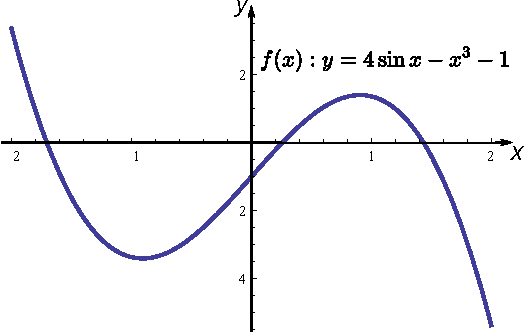
\includegraphics[scale=1]{mai_fig035.pdf}
           \captionof{figure}{Graf funkce $f(x):y=4\sin x - x^3 - 1$.}
           \label{mai:fig035}
           \par}
        Z obrázku \ref{mai:fig035} zjistíme, že existují tři kořeny: $x_1^*\in(-2,-1),
        x_2^*\in(-1, 0)$ a $x_3^*\in(1, 2)$.
      \end{example}
  
      Z obrázku zjistíme, že existují tři kořeny: $x_1^*\in(-2,-1),x_2^*\in(0,1),x_3^*\in(1,2)$.
      Zkusme najít kořeny v těchto intervalech pomocí numerických metod popsaných v následujících
      odstavcích
  
    \subsection{Metoda bisekce}
      Metoda známá také jako \textbf{metoda půlení intervalů}, je založena na principu
      zna\-mén\-ko\-vých změn. Předpokládejme, že funkce $f(x)$ má v koncových bodech intervalu
      $(a_0,b_0)$ opačná znaménka, tj. platí $f(a_0 )\cdot f(b_0 )<0$. Sestrojíme posloupnost
      intervalů $(a_1,b_1)\supset(a_2,b_2)\supset(a_3,b_3)\supset\cdots$, které obsahují kořen.
      Intervaly $(a_{k+1},b_{k+1}), k=0,1,\cdots$, určíme rekurzivně způsobem, který si nyní
      popíšeme.
  
      Střed intervalu $(a_k,b_k)$ je bod $x_{k+1}=\frac{1}{2}(a_k+b_k)$. Když $f(x_k)=0$, pak
      $x_{k+1}=x^*$ je kořen a dál nepokračujeme.

%} %tikzset
%---------------------------------------------------------------------------------------------------
\printbibliography[heading=subbibliography]
\addcontentsline{toc}{section}{Seznam literatury}
%  % !TeX spellcheck = cs_CZ
%     An overview of high school mathematics
%{\tikzset{external/prefix={tikz/MAI/}}
% \tikzset{external/figure name/.add={ch01_}{}}
%---------------------------------------------------------------------------------------------------
% history_MA.tex
%---------------------------------------------------------------------------------------------------
\setchaptertoc
\chapter{Historie matematické analýzy} %\label{mai:IchapI}

  Analýza jako nezávislý předmět byla vytvořena v 17. stol. během vědecké revoluce. Kepler, 
  Galilei, Descartes, Fermat, Huygens, Newton a Leibniz, když zmíníme jen několik důležitých jmen 
  těch, kteří přispěli k jejímu vzniku. Otázky z mechaniky, optiky a astronomie hráli roli v jejím 
  raném období, tak jako vnitřní problémy matematiky, jako výpočet obsahů, objemů a analýza 
  komplikovaných křivek. Pohyb po zakřivených drahách působením proměnných sil, které se staly 
  předmětem důkladného zájmu po studiu volně padajících těles Galilea, vedl k počátečnímu úspěchu. 
  Z velké rozmanitosti snah, které se objevily na konci 17. stol. v práci Newtona a Leibnize, se 
  zrodila nová matematická disciplína, jejíž některé poznatky jsou v těchto studijních zápiscích.
  
  Základní myšlenka použití diferenciálních rovnic k získání pohledu na globální chování proměnných
  kvantit z jejich (infinitezimálních) změn prokázala základní a plodné výsledky daleko za hranicemi
  matematiky a fyzika a formovala náš souhrnný vědecký pohled na svět, zvláště na představu o
  kauzalitě. Na konci 18. stol., vskutku, největší vědci došli ke shodě, že procesy v přírodě (a
  společnosti) jsou determinovány a podřízeny zákonům, které mohou být popsány v podobě
  diferenciálních rovnic. Laplace, tento mistr matematické fyziky, naznačil obraz nějaké fiktivní
  vševědoucí inteligence, užívající úplnou znalost zákonů a stavu světa v daný časový okamžik, by
  mohla předpovídat další vývoj světa navždy a hned. Myšlenka \emph{přírodních zákonů} byla kmotrem
  při vytvoření matematického pojmu funkce a naopak nebyla by to myšlenka nikdy tak vlivná, kdyby
  matematická analýza nevyvíjela úspěšné metody pro výzkum funkčních závislostí. 

%} % tikzset
%---------------------------------------------------------------------------------------------------              
}
{
% DEBUG was off
%---------------------Reálná a komplexní čísla-----------------------------------------------------
  % !TeX spellcheck = cs_CZ
% Basis of Linear Algebra:
%{\tikzset{external/prefix={tikz/MAI/}}
% \tikzset{external/figure name/.add={ch02_}{}}
%---------------------------------------------------------------------------------------------------
% intro_linear_algebra.tex
%---------------------------------------------------------------------------------------------------
% ==================================================================================================
% In linear algebra, a basis is a set of linearly independent vectors that, in a
% linear combination, can represent every vector in a given vector space or free
% module, or, more simply put, which define a "coordinate system".[1] In more
% general terms, a basis is a linearly independent spanning set. 
% --------------------------------------------------------------------------------------------------
\chapter{Všemocná úměra aneb lineární algebra poprvé}\label{mai:IchapII}
\minitoc
  Tuto kapitolu bychom mohli opatřit podtitulem \emph{„To nejnutnější z lineární algebry“}. 
  Dovíme se v ní, co je třeba si představit pod pojmem \emph{„linearita“}, najdeme příklady 
  linearity v geometrii i v přírodovědě (fyzice, chemii, biologii) a formulujeme základní 
  poznatky týkající se řešení soustav lineárních rovnic. Do této oblasti patří i počítání s 
  vektory a maticemi - objekty, které jsou velmi vhodné k vyjádření fyzikálních veličin.
    
  \section{Lineární rovnice}\label{mai:IchapIIsecI}
    Co tedy znamená slovo \textbf{linearita}? Pochází z latiny, \emph{linea recta = přímka}, 
    česky bychom řekli \emph{přímá úměrnost} nebo jen jednoduše \emph{úměra}.
    
    Nejjednodušší příklady linearity patří do oblasti geometrie - vyjádření \emph{přímek} a 
    \emph{rovin}. Jistě si ze střední školy vzpomínáme, že body těchto útvarů popisujeme jejich 
    souřadnicemi na přímce \(\mathbb{R}\), v rovině \(\mathbb{R}^2\), v prostoru \(\mathbb{R}^3\). 
    Souřadnice bodu v rovině tedy tvoří \emph{uspořádanou dvojici} reálných čísel, v prostoru pak 
    \emph{uspořádanou trojici} reálných čísel. (Pozor, dvojice \([a, b]\) a \([b, a]\) představují 
    různé body.)

    %--Parametrické vyjádření přímky--------------------------------
        % !TeX spellcheck = cs_CZ
% Musilova2009MA1
\wikitextrule
\begin{example}\label{mai:exam001}
  \textbf{Parametrické vyjádření přímky}\newline\small
  \emph{Přímka} — jednorozměrný lineární útvar v jednorozměrném prostoru \(\mathbb{R}^1\), 
  dvojrozměrném prostoru \(\mathbb{R}^2\), trojrozměrném prostoru \(\mathbb{R}^3\) (nebo i 
  n-rozměrném prostoru \(\mathbb{R}^n\)), je určena dvěma body, třeba \(A\) a \(B\), nebo 
  ekvivalentně, bodem \(A\) a \emph{směrovým} vektorem \(\vec{u}\) (obr. \ref{mai:fig000}). 
  Je-li \(X\) obecným bodem na této přímce, je vektor \(\overrightarrow{AX}\) rovnoběžný, 
  tj. \emph{kolineární}, se směrovým vektorem \(\vec{u}\). (Jako směrový můžeme samozřejmě 
  použít i vektor \(\overrightarrow{AB}\).) Vektor \(\overrightarrow{AX}\) má tedy s 
  vektorem \(\vec{u}\) stejný směr, lišit se může velikostí nebo orientací. Tuto skutečnost 
  zapíšeme tak, že \(\overrightarrow{AX}\) je \(t\)-násobkem vektorů \(\vec{u}\),
  \begin{equation*}
  \overrightarrow{AX} = t \cdot \vec{u}.
  \end{equation*}
  {\centering
    \captionsetup{type=figure}
    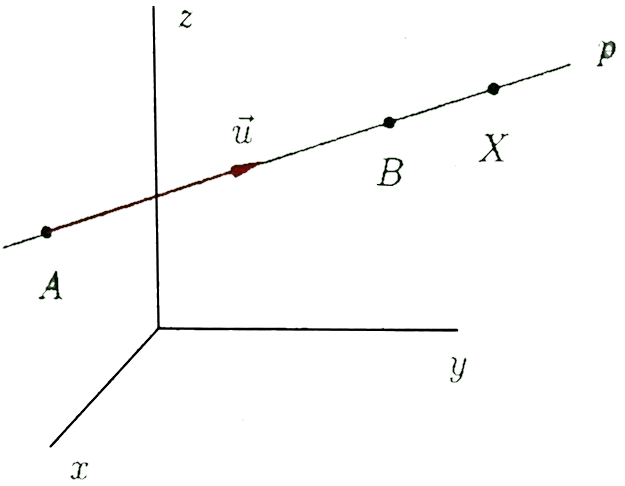
\includegraphics[width=0.4\linewidth]{mai_fig000.png}
    \captionof{figure}{Zadáni přímky. \cite[s.~1]{Musilova2009MA1}
    \label{mai:fig000}}
    \par}
  Veličinou \(t\), takzvaným \emph{parametrem}, který může nabývat všech reálných hodnot, 
  \(t\in\mathbb{R}\), dokážeme popsat všechny vektory \(\overrightarrow{AX}\), jejichž 
  koncový bod \(X\) leží na přímce \(p\). Naopak, žádné jiné body \(X\) než ty, které leží na 
  přímce \(p\), tuto vlastnost nemají. S označením bodů \(A\), \(X\), resp. vektorů 
  \(\vec{u}\), \(\overrightarrow{AX}\) kartézskými souřadnicemi, resp. složkami
  \begin{align*}
                    A &= (x_A,y_A, z_A), \\ 
                    X &=(x,y,z),         \\
              \vec{u} &= (u_1,u_2,u_3),  \\ 
  \overrightarrow{AX} &= (x - x_A, y - y_1A, z-z_A),
  \end{align*}
  dostáváme \textbf{parametrické vyjádřeni přímky} \(p\) ve tvaru
  \begin{equation}\label{MAI:eq_M001}
    p = \left\{(x,y,z)\in\mathbb{R}^3\,|\,
    \begin{matrix}
      x = x_A + tu_1,        \\
      y = y_A + tu_2,        \\
     z = z_A + tu_3,
    \end{matrix}
    \;t\in\mathbb{R}
    \right\}. 
  \end{equation}
  \normalsize
\end{example}
    %---------------------------------------------------------------
    
    Vidíme, že kartézské souřadnice bodu na přímce se vůči souřadnicím bodu \(A\) mění přímo 
    úměrně v závislosti na hodnotě parametru \(t\), tj. závisí na jeho první mocnině. Příslušná 
    závislost se nazývá \textbf{lineární funkcí}.
    
    Obdobně zapíšeme parametrické vyjádření roviny v \(\mathbb{R}^3\):
    
    %--Parametrická vyjádření roviny--------------------------------
    % !TeX spellcheck = cs_CZ
\begin{mathexam}{Parametrická vyjádření roviny}{exam004}
  Rovina v trojrozměrném prostoru \(\mathbb{R}^3\) je zadána třemi body \(A\), \(B\) a \(C\), které
  nesmějí ležet v jedné přímce, popřípadě dvěma body \(A\) a \(B\) a vektorem \(\vec{v}\)
  nerovnoběžným s \(\overrightarrow{AB}\), anebo bodem \(A\) a dvěma nerovnoběžnými směrovými
  vektory \(\vec{u}\) a \(\vec{v}\) (obr. \ref{mai:FIG002}). Všechny tyto typy zadání jsou
  ekvivalentní. Lze volit například \(\vec{u} = \overrightarrow{AB}\), \(\vec{v} =
  \overrightarrow{AC}\). Je-li \(X\) libovolným bodem roviny \(\varrho\), jsou vektory
  \(\overrightarrow{AX}\), \(\vec{u}\) a \(\vec{v}\) \textbf{lineárně závislé}. To znamená, že
  existují taková reálná čísla \(r\) a \(s\), že vektor \(\overrightarrow{AX}\) lze zapsat jako
  lineární kombinaci

  \begin{equation*}
    \overrightarrow{AX} = r\cdot\vec{u} + s\cdot\vec{v}, \qquad r,s \in\mathbb{R}
  \end{equation*}
  Při obdobném zápisu kartézských souřadnic bodů a složek vektorů jako u vyjádření přímky dostaneme
  parametrické vyjádření roviny \(\varrho\)
  \begin{equation*}
    \varrho = \left\{
    \begin{matrix}  
      (x,y,z)\in\mathbb{R}^3  \\
      r, s \in\mathbb{R}
    \end{matrix}
    \,\left\lvert\,
    \begin{matrix}
      x = x_A + ru_1 + sv_1,        \\
      y = y_A + ru_2 + sv_2,        \\
      z = z_A + ru_3 + sv_3,
    \end{matrix}\right.          
    \right\}.
  \end{equation*} 

  { \centering
    \captionsetup{type=figure}
    \luafigure[1]{mai_fig026.pdf}
    \captionof{figure}{Zadání roviny. \cite[s.~3]{Musilova2009MA1}
    \label{mai:FIG002}} \par}

  Toto vyjádření obsahuje opět lineární závislost: Souřadnice \(x\), \(y\) a \(z\) se vůči
  souřadnicím bodu \(A\) mění v závislosti na prvních mocninách parametrů \(r\) a \(s\). Můžeme tak
  hovořit o jakési „vícerozměrné úměře“.
\end{mathexam}
  
    %---------------------------------------------------------------
    
    Všimněme si nyní příkladů linearity z oblasti přírodovědy.
    
    %--Fyzika — Ohmův zákon-----------------------------------------
    % !TeX spellcheck = cs_CZ
% \wikitextrule
\begin{mdframed}[style=mdexam]
  \begin{example}\label{mai:exam035}
    \textbf{Fyzika - Ohmův zákon:}\newline
    Z elektřiny víme, že některé vodiče či elektrické prvky se při průchodu elektrického proudu 
    chovají podle zákona linearity: Proud, který jimi protéká, závisí přímo úměrně na přiloženém 
    napětí (obr. \ref{mai:fig036}). Platí \(I(U) = R^{-1 }U\) s konstantou úměrnosti \(R^{-1}\), kde 
    \(R\) je elektrický odpor vodiče (prvku).

    Pozn. 1: Předpokládáme, že elektrický odpor voltmetru je tak velký, že proud jím procházející je 
    z hlediska přesnosti měření zanedbatelný.
    
    Pozn. 2: Graf závislosti proudu na napětí na obrázku \ref{mai:fig036} může pro vyšší hodnoty 
    napětí vykazovat odchylku od linearity (přímkové závislosti), neboť se prvek při vyšším proudu 
    zahřívá a jeho odpor roste.
    
    {\centering
      \captionsetup{type=figure}
      \luafigure[1]{mai_fig036.png}
      \captionof{figure}{Chování lineárního vodiče (Ohmův zákon). \cite[s.~15]{Musilova2009MA1}
      \label{mai:fig036}}
      \par}  
  \end{example}
\end{mdframed}
    %---------------------------------------------------------------

    %--Fyzika — speciální typy pohybů-------------------------------
    % !TeX spellcheck = cs_CZ
\wikitextrule
\begin{example}\label{mai:exam036}
  \textbf{Fyzika — speciální typy pohybů:}\newline\small
  Při rovnoměrném pohybu tělesa (ať již přímočarém či křivočarém) je dráha, kterou těleso urazí za 
  dobu \(t\), přímo úměrná velikosti jeho rychlosti \(v\), tj. \(s(t) = s_0 + vt\). Při pohybu 
  rovnoměrně zrychleném (zpožděném) je lineární závislost velikosti rychlosti na čase, tj. \(v(t) = 
  v_0 \pm at\) při pohybu přímočarém (\(a\) je velikost zrychlení), nebo \(v(t) = v_0 \pm a_\tau 
  t\) při pohybu křivočarém (\(a_\tau\) je velikost průmětu zrychlení do směru tečny k 
  trajektorii tělesa — tečného zrychlení).
  \normalsize
\end{example}
    %---------------------------------------------------------------
    
  \subsection{Soustavy lineárních rovnic a jejich rychlé řešení}
    Příkladů linearity v přírodě bychom mohli nalézt bezpočet. Vraťme se však k matematice a k 
    problematice uvedené v názvu tohoto odstavce, k soustavám lineárních rovnic. Začněme 
    jednoduchou slovní úlohou ze základní školy:
    
    %--Jeníček a Mařenka kradli ježibabě perník---------------------
    % !TeX spellcheck = cs_CZ
% \wikitextrule
\begin{mdframed}[style=mdexam]
  \begin{example}\label{mai:exam037}
    \textbf{Jeníček a Mařenka kradli ježibabě perník:}\newline
    Dohromady snědli \num{11} perníkových srdíček. Jeníček jich přitom zkonzumoval o \num{3} více
    než Mařenka. Otázka je tradiční - kolik srdíček snědl každý z nich? Označíme-li \(M\) počet
    kousků, které snědla Mařenka a \(J\) počet srdíček, na nichž si pochutnal Jenda, můžeme
    informace zadané v úloze zapsat takto:
    \begin{equation*}
      M + J = 11, \qquad J = M + 3.
    \end{equation*}
    
    Řešení není problémem, snadno vidíme, že \(M = 4\) a \(J = 7\).
  \end{example}
\end{mdframed}
    %---------------------------------------------------------------
    
    O samotné řešení této jednoduché úlohy v tuto chvíli nejde. Pojmenujme si však vztahy, které 
    jsme pro neznámé hodnoty \(M\) a \(J\) ze zadání úlohy dostali. Neznámé vystupují v 
    rovnicích v první mocnině, tedy \emph{lineárně}. Máme \emph{soustavu dvou rovnic} o dvou 
    neznámých \(M\) a \(J\). Úvahu snadno zobecníme: Předpokládejme, že máme neznámé veličiny
    \begin{equation*}
      (x_1, x_2, \ldots, x_n)
    \end{equation*}
    a máme o nich \(m\) informací, které lze zapsat ve tvaru lineárních rovnic (neznámé budou v 
    těchto rovnicích vystupovat v první mocnině),
    \begin{align}
      a_{11}x_1 + a_{12}x_2 + \ldots + a_{1n}x_n &= b_1,     \nonumber           \\
      a_{21}x_1 + a_{22}x_2 + \ldots + a_{2n}x_n &= b_2,     \label{mai:eq002}   \\
      .......................................... &= \ldots   \nonumber           \\
      a_{m1}x_1 + a_{m2}x_2 + \ldots + a_{mn}x_n &= b_m,     \nonumber
    \end{align}
    Soustavu (\ref{mai:eq002}) nazýváme soustavou \(m\) lineárních rovnic o \(n\) neznámých. 
    Označme ji jako \(S\) a pod tímto označením se k ní budeme vracet. Soubory reálných čísel 
    \((a_{ij})\) a \((b_i)\), kde \(1 < i < m\), \(1 \leq j < n\), jsou zadány. Lze je uspořádat 
    do takzvaných \textbf{matic}:
    \begin{equation}\label{mai:eq003}
      \matr{A} =
        \begin{pmatrix}
          a_{11} & a_{12} & \ldots & a_{1n} \\
          a_{21} & a_{22} & \ldots & a_{2n} \\
          \ldots & \ldots & \ldots & \ldots \\
          a_{m1} & a_{m2} & \ldots & a_{mn}          
        \end{pmatrix},
        \overline{\matr{B}} =
        \begin{pmatrix}
          b_1     \\
          b_2     \\
          \ldots  \\
          b_m 
        \end{pmatrix}
    \end{equation}
    
    Matice \(\matr{A}\) je typu \(m/n\), má \(m\) řádků a \(n\) sloupců, \(i\) je řádkový index a 
    \(j\) je sloupcový index. Matice \(\overline{\matr{B}}\) je typu \(m/1\) (\(m\) řádků a jeden 
    sloupec), hovoříme také o sloupcové matici. Soustavu \(S\) můžeme zapsat zkráceně pomocí 
    maticového násobení (podrobněji viz později odstavec \ref{mai:IchapIIsecIII}):
    \begin{equation*}
      \matr{A} \cdot \matr{X} = \matr{B}, \qquad \text{nebo}
    \end{equation*}  
    \begin{equation}\label{mai:eq004}
        \begin{pmatrix}
          a_{11} & a_{12} & \ldots & a_{1n} \\
          a_{21} & a_{22} & \ldots & a_{2n} \\
          \ldots & \ldots & \ldots & \ldots \\
          a_{m1} & a_{m2} & \ldots & a_{mn}
        \end{pmatrix}
        \cdot
        \begin{pmatrix}
          x_1     \\
          x_2     \\
          \ldots  \\
          x_m 
       \end{pmatrix}
        =
       \begin{pmatrix}
            b_1     \\
            b_2     \\
            \ldots  \\
            b_m 
          \end{pmatrix}
    \end{equation}
    V tuto chvíli vysvětlíme podstatu maticového násobení jen technicky: Násobit mezi sebou  můžeme matici 
    \(\matr{A} = (a_{ij})\) typu \(m/n\) (levý činitel) a matici \(\matr{A} = (c_{jk})\) typu 
    \(n/p\) (pravý činitel, činitele nelze zaměňovat). Výsledkem je matice \(\matr{A} = (d_{ik})\) 
    typu \(m/p\), jejíž prvky se počítají podle předpisu
    \begin{equation}\label{mai:eq005}
      d_{ik} = \sum_{j=1}^{n} a_{ij}\cdot c_{jk}.
    \end{equation}
    
    Z tohoto obecného předpisu vidíme, že levé strany soustavy \(S\) lze interpretovat ve tvaru 
    součinu matice \(A\) typu \(m/n\) s maticí neznámých typu \((n/1)\), výsledkem je matice 
    pravých stran \(\overline{\matr{B}}\), která je typu \(m/1\). Matice \(\matr{A}\) se nazývá 
    \textbf{maticí soustavy}. Matice, která vznikne jejím \emph{rozšířením} o sloupec pravých 
    stran, tj.
    \begin{equation}\label{mai:eq006}
      \matr{B} = (\matr{A}|\overline{\matr{B}}) =
      \left(
        \begin{array}{cccc|c}
          a_{11} & a_{12} & \ldots & a_{1n} & b_1    \\
          a_{21} & a_{22} & \ldots & a_{2n} & b_2    \\
          \ldots & \ldots & \ldots & \ldots & \ldots \\
          a_{m1} & a_{m2} & \ldots & a_{mn} & b_m
        \end{array}
      \right)
    \end{equation}
    je pak \textbf{rozšířenou maticí soustavy}. Je-li sloupec pravých stran soustavy tvořen 
    samými nulami, nazývá se soustava \textbf{homogenní}, v opačném případě \textbf{nehomogenní}. 
    Řešením soustavy \(S\) nazýváme každou \(n\)-tici \((x_i, x_2,\ldots, x_n)\), která soustavu 
    \(S\) splňuje. Cílem je najít všechna řešení soustavy \(S\). Abychom řešení nalezli, musíme 
    soustavu upravovat, zjednodušovat. Prováděné úpravy mají vést k jednodušší, avšak 
    ekvivalentní soustavě rovnic, tj. takové, která má naprosto stejný soubor všech řešení jako 
    soustava původní. Takové úpravy nazýváme \textbf{ekvivalentními}. Dvě základní, pomocí nichž 
    lze uskutečnit všechny ostatní, jsou
    \begin{itemize}\addtolength{\itemsep}{-0.5\baselineskip}
      \item vynásobení libovolné, například \(i\)-té, rovnice libovolným \emph{nenulovým} číslem,
      \item přičtení \(i\)-té rovnice vynásobené libovolným číslem k \(l\)-té rovnici.
    \end{itemize} 
    V soustavě lze samozřejmě také měnit pořadí rovnic. Tato úprava je rovněž ekvivalentní. 
    Nevypisujeme ji však zvlášť proto, že ji lze realizovat pomocí vhodně zvolené posloupnosti 
    základních dvou úprav.
    
    Abychom nemuseli soustavu stále opisovat i s neznámými, provádíme obvykle ekvivalentní 
    úpravy jen s maticí \(\matr{B} = (\matr{A}|\overline{\matr{B}})\) (každý řádek této matice 
    představuje jednu rovnici soustavy \(S\)). Může se stát, že soustava má právě \emph{jedno 
    řešení}, jako tomu bylo v  úloze o Mařence a Jeníčkovi. Také nemusí mít \emph{řešení žádné}, 
    jako například soustava \(x + y = 0\), \(x + y = 1\) (součet dvou čísel nemůže nabývat současně 
    dvou různých hodnot). A třeba má také řešení \emph{nekonečně mnoho} (řešením soustavy jedné 
    rovnice o dvou neznámých \(x + y = 1\) jsou všechny dvojice tvaru \((x, 1 - x)\), kde \(x\) je 
    libovolné). A může mít soustava \(S\) třeba právě dvě řešení? Prostřednictvím následujícího 
    příkladu ukážeme metodu, která vede velmi rychle k nalezení všech řešení a umožňuje také 
    vyslovit obecné závěry o jejich vlastnostech a počtu. Jedná se o \textbf{Gaussovu eliminační 
    metodu}.

    %Gaussova eliminační metoda-------------------------------------
    \begin{mathexam}{Gaussova eliminační metoda}{exam038}
  Je zadána soustava tří (\(m = 3\)) rovnic o pěti (\(n = 5\)) neznámých:
  \begin{alignat*}{7}
       x_1 &+ 2x_2 &-  x_3 &+  x_4 &- 5x_5 &=  &&0, \\
     -2x_1 &- 4x_2 &+ 2x_3 &+ 4x_4 &+ 4x_5 &= -&&6, \\
      -x_1 &- 2x_2 &+  x_3 &+ 5x_4 &-  x_5 &=  &&6.
  \end{alignat*}
  Budeme provádět ekvivalentní úpravy matice \(\matr{B}\) tak, abychom ji zjednodušovali.
  Ekvivalenci matic budeme označovat znakem \(\sim\). 
  \begingroup
    \renewcommand\arraystretch{1.0}
    \renewcommand\arraycolsep{3pt}
    \begin{equation*}
      \matr{B} = (\matr{A}\lvert\overline{\matr{B}}) =
      \left(
        \begin{array}{rrrrr|r}
           1 &  2 & -1 & 1 & -5 &  0    \\
          -2 & -4 &  2 & 4 &  4 & -6    \\
          -1 & -2 &  1 & 5 & -1 &  6
        \end{array}
      \right).
    \end{equation*}
  \endgroup
  V prvním řádku je na první pozici jednička. Toho využijeme k snadné „likvidaci“, tedy eliminaci,
  prvních prvků v druhém a třetím řádku pomocí elementárních úprav. Provedeme tyto dvě úpravy:
  první řádek vynásobený číslem \num{2} přičteme k druhému řádku, první řádek přičteme ke třetímu
  řádku. Dostaneme
  \begingroup
    \renewcommand\arraystretch{1.0}
    \renewcommand\arraycolsep{3pt}
    \begin{equation*}
      \matr{B} \sim
      \left(
        \begin{array}{rrrrr|r}
          1 &  2 & -1 & 1 & -5 &  0         \\
          \bm{0} &  0 &  0 & 6 & -6 & -6    \\
          \bm{0} &  0 &  0 & 6 & -6 &  6
        \end{array}
      \right).
    \end{equation*}
  \endgroup  
  Vidíme, že jsme v druhém i třetím řádku dostali na první sloupcové pozici nulu (tučná). (Nuly na
  dalších  pozicích vznikly náhodou, vlivem jednoduchosti zadání.) Nyní vynásobíme druhý i třetí
  řádek číslem (\num{1/6}):
  \begingroup
    \renewcommand\arraystretch{1.0}
    \renewcommand\arraycolsep{3pt}    
    \begin{equation*}
      \matr{B} \sim
      \left(
        \begin{array}{rrrrr|r}
                1 &  2 & -1 & 1 & -5 &  0    \\
                0 &  0 &  0 & 1 & -1 & -1    \\
                0 &  0 &  0 & 1 & -1 &  1
        \end{array}
      \right).
    \end{equation*}
  \endgroup  
  Přestože již nyní vidíme, že soustava nemá řešení (rovnice druhého a třetího řádku znějí \(x_4 -
  x_5 = - 1\) a \(x_4 -x_5 = 1\), takže jim nevyhovuje žádná dvojice čísel \((x_4, x_5)\)), budeme
  v eliminaci pokračovat. Další úpravy se již týkají pouze druhého a třetího řádku. Druhý řádek
  vynásobený (\num{-1}) přičteme ke třetímu. Pak

  \begingroup
  \renewcommand\arraystretch{1.0}
  \renewcommand\arraycolsep{3pt}
    \begin{equation*}
      \matr{B} \sim
      \left(
        \begin{array}{rrrrr|r}
                1 &  2 & -1 & 1      & -5 &  0    \\
                0 &  0 &  0 & 1      & -1 & -1    \\
                0 &  0 &  0 & \bm{0} &  0 &  2
        \end{array}
      \right).
    \end{equation*}
  \endgroup  
  Získáváme tak ekvivalentní soustavu rovnic
  \begin{alignat*}{5}
        x_1 + 2x_2 - x_3 &+  x_4 &- 5x_5 &=  &&0, \\
                         &+  x_4 &-  x_5 &= -&&1, \\
                         &       &     0 &=  &&2.
  \end{alignat*}
  V poslední rovnici je ihned vidět rozpor - soustava nemá řešení
\end{mathexam}
    %---------------------------------------------------------------

    Na základě výsledného tvaru matice soustavy a rozšířené matice soustavy získané ekvivalentními 
    úpravami soustavy \(S\) nyní formulujeme obecné kritérium pro to, aby soustava S měla
    vůbec nějaké řešení. Matice \(\matr{A}\) i \(\matr{B}\) se po provedení ekvivalentních úprav 
    dostaly do velmi jednoduchého tvaru, který připomíná schodiště obrácené „vzhůru nohama“, 
    odmyslíme-li si nuly v levé části jednotlivých řádků (následující zápis pouze usnadňuje 
    názornou představu, znak ekvivalence již psát nemůžeme):
    \begin{equation*}
      \matr{A} \ldots
      \left(
        \begin{array}{rrrrr}
                1 &  2 & -1 & 1      & -5     \\
                  &    &    & 1      & -1     \\
 
        \end{array}
      \right),
      \qquad
      \matr{B} \ldots
      \left(
        \begin{array}{rrrrr|r}
                1 &  2 & -1 & 1      & -5 &  0    \\
                  &    &    & 1      & -1 & -1    \\
        \end{array}
      \right).
    \end{equation*}
    
    Všimněme si, že „schodiště“ jsou nepravidelná, pokud jde o šířku schodů, výška všech schodů
    je však stejná - jeden řádek. Tímto způsobem je dán \emph{schodovitý tvar} matice \(\matr{A}\), 
    resp. \(\matr{B}\). Úzce s ním souvisí důležitá charakteristika matice, která je nezávislá jak 
    na provedených úpravách tak na výsledném schodovitém tvaru. Je to hodnost matice, definovaná 
    takto:
    
    \textbf{Hodnost} matice je počet nenulových řádků jejího schodovitého tvaru.
    
    V našem příkladu je hodnost matice \(A\) soustavy \(S\) rovna dvěma, hodnost matice rozšířené 
    \(\matr{B}\) je rovna třem. Píšeme
    \begin{equation*}
      h(\matr{A}) = 2,\qquad h(\matr{B}) = 3.
    \end{equation*}
    
    \begin{note}
      Lze získat schodovitý tvar různými posloupnostmi ekvivalentních úprav je zřejmé. Uvědomme si 
      však, že ani výsledný schodovitý tvar není určen jednoznačně - stačí třeba vynásobit některý 
      řádek dvěma a výsledná matice ekvivalentní s původní je rovněž schodovitá. Poněvadž má matice 
      \(\matr{B}\) o jeden sloupec více než matice \(\matr{A}\), platí vždy \(h(\matr{A}) < 
      h(\matr{B})\). V případě \(h(\matr{A}) < h(\matr{B})\) pak \(h(\matr{A}) = h(\matr{B}) - 1\). 
      Jak názorně ukazuje náš příklad, má pro \(h(\matr{A}) < h(\matr{B})\) některá z rovnic 
      ekvivalentní soustavy tvar \(0 = 1\), soustava tedy nemá řešení. Můžeme tak formulovat 
      kritérium (podmínku nutnou a postačující) řešitelnosti soustavy lineárních rovnic.
    \end{note}
    
    \begin{lemma}\label{mai:lemma001}
      (\textbf{Frobeniova}): Soustava lineárních rovnic má řešení právě tehdy, je-li hodnost její 
      matice rovna hodnosti matice rozšířené.
    \end{lemma}
    
    Ihned vidíme, že homogenní soustava má podle této věty řešení vždy, neboť poslední sloupec její 
    rozšířené matice je složen ze samých nul. Skutečně, jedním ze souboru řešení každé
    homogenní soustavy je \(n\)-tice
    \begin{equation*}
      (x_1, x_2, \ldots, x_n) = (0, 0, \ldots, 0),
    \end{equation*}
    zvaná \textbf{triviální řešení}.
    
    Nyní se vraťme k otázce, jak zjistit, kolik řešení má daná soustava, a jak je všechna popsat.
    Poslouží nám příklad \ref{mai:exam038} v mírné obměně spočívající v záměně koeficientu \(b_3\) 
    z hodnoty \num{6} na \num{-6}.
    
    %Ještě jednou Gaussova eliminační metoda------------------------
    % !TeX spellcheck = cs_CZ
\wikitextrule
\begin{example}\label{mai:exam039}
  \textbf{Ještě jednou Gaussova eliminační metoda}\newline\small
  Je zadána soustava rovnic:
  \begin{alignat*}{7}
      x_1 &+ 2x_2 &-  x_3 &+  x_4 &- 5x_5 &=  &&0, \\
    -2x_1 &- 4x_2 &+ 2x_3 &+ 4x_4 &+ 4x_5 &= -&&6, \\
     -x_1 &- 2x_2 &+  x_3 &+ 5x_4 &-  x_5 &= -&&6.
  \end{alignat*}
  Rozšířená matice soustavy má nyní tvar 
  \begin{equation*}
    \matr{B} = (\matr{A}|\overline{\matr{B}}) =
    \left(
      \begin{array}{rrrrr|r}
         1 &  2 & -1 & 1 & -5 &  0    \\
        -2 & -4 &  2 & 4 &  4 & -6    \\
        -1 & -2 &  1 & 5 & -1 & -6
      \end{array}
    \right).
  \end{equation*}
  Stejné ekvivalentní úpravy jako v příkladu \ref{mai:exam038} vedou nyní k výsledku
  \footnotesize %\small \scriptsize \tiny
  \begin{equation*}
    \matr{B} \sim
    \left(
      \begin{array}{rrrrr|r}
         1 &  2 & -1 & 1 & -5 &  0         \\
         \bm{0} &  0 &  0 & 6 & -6 & -6    \\
         \bm{0} &  0 &  0 & 6 & -6 & -6
      \end{array}
    \right) \sim
    \left(
      \begin{array}{rrrrr|r}
              1 &  2 & -1 & 1 & -5 &  0    \\
              0 &  0 &  0 & 1 & -1 & -1    \\
              0 &  0 &  0 & 1 & -1 & -1
      \end{array}
    \right) \sim
    \left(
      \begin{array}{rrrrr|r}
              1 &  2 & -1 & 1      & -5 &  0    \\
              0 &  0 &  0 & 1      & -1 & -1    \\
              0 &  0 &  0 & \bm{0} &  0 &  0
      \end{array}
    \right).
  \end{equation*}\normalsize
  Nyní platí \(h(\matr{A}) = h(\matr{B}) = 2\). Podle Frobeniovy věty \ref{mai:lemma001} tedy 
  soustava určitě má řešení. Ekvivalentní soustava má tvar
  \begin{alignat*}{5}
         x_1 + 2x_2 - x_3 &+  x_4 &- 5x_5 &=  &&0, \\
                          &+  x_4 &-  x_5 &= -&&1, \\
                          &       &     0 &=  &&0.
  \end{alignat*}
  Poslední rovnice je identitou a můžeme ji vypustit. Máme pět neznámých a jen dvě nezávislé 
  rovnice. Dvě z neznámých tedy můžeme vyjádřit pomocí zbývajících. Postupujeme „odzadu“ , začínáme 
  druhou, jednodušší, rovnicí:
  \begin{align*}
                                                x_4 &= -1 + x_5,                \\
    x_1 = - 2x_2 + x_3 - x_4 + 5x_5 \Rightarrow x_1 &= -2x_2 + x_3 + 4x_5 + 1.
  \end{align*}
  Za neznámé vystupující na pravé straně, tj. \(x_2\), \(x_3\) a \(x_5\), můžeme dosazovat cokoli a 
  vždycky se k nějakým hodnotám \(x_1\) a \(x_4\) dopočítáme. Všechna řešení soustavy \(S\) proto 
  můžeme zapsat v obecném tvaru
  \begin{equation}\label{mai:eq040}
    (-2x_2 + x_3 + 4x_5 + 1, x_2, x_3, x_5 - 1, x_5).
  \end{equation}
  \normalsize
\end{example}
    %---------------------------------------------------------------
    
    Soubor řešení ve tvaru (\ref{mai:eq040}) se nazývá obecným řešením soustavy. Jeho jednotlivé 
    prvky, jednotlivá konkrétní řešení soustavy, jsou dány volbou volných neznámých \(x_2\), 
    \(x_3\) a \(x_5\). Také z příkladu \ref{mai:exam039} lze učinit obecný závěr:
    
    \begin{lemma}\label{mai:lemma002}
      Nechť pro soustavu \(m\) lineárních rovnic o \(n\) neznámých platí \(h(\matr{A}) = 
      h(\matr{B}) = h\). Pak její obecné řešení závisí (lineárně) na \(d = n - h\) volných 
      neznámých.
    \end{lemma}
    
    Číslo \(d\) se nazývá \textbf{dimenze prostoru řešení soustavy}. Tento pojem ještě podrobněji 
    vysvětlíme později.
    
    Nyní již snadno zodpovíme otázku, čím je dána mohutnost souboru řešení soustavy lineárních 
    rovnic, tj. kolik má taková soustava řešení. Možnosti jsou pouze:
    \begin{itemize}
      \item žádné řešení - pro \(h(\matr{A}) \neq h(\matr{B})\),
      \item právě jedno řešení - pro \(h = h(\matr{A}) = h(\matr{B})\) a současně \(h = n\), takže 
            nezbývá žádná volná neznámá,
      \item nekonečně mnoho řešení - pro \(h = h(\matr{A}) = h(\matr{B})\) a současně \(h < n\),  
            kdy máme k dispozici \(d = n - h\) volných neznámých.
    \end{itemize}    
    Že by tedy třeba měla soustava právě dvě, tři či osmnáct řešení není možné.
    
    Jakési zvláštní postavení můžeme přisoudit homogenním soustavám. Ty mají, jak jsme se
    již přesvědčili, řešení vždy, alespoň to triviální, složené ze samých nul. Zajímejme se o 
    situaci, kdy má homogenní soustava i jiná, netriviální, řešení. U homogenní soustavy je 
    hodnost její matice vždy shodná s hodností matice rozšířené, \(h = h(\matr{A}) = h(\matr{B})\). 
    Je-li navíc \(h = n\), má podle obecného tvrzení \ref{mai:lemma002} soustava právě jedno 
    řešení, jímž nutně je řešení triviální. V opačném případě, tj. pro \(h < n\), máme opět k 
    dispozici \(d = n - h\) volných neznámých, a tedy nekonečně mnoho netriviálních řešení. 
    Všimněme si ještě jedné zajímavosti u homogenní soustavy. Jsou-li dvě \(n\)-tice čísel \(X = 
    (x_1, x_2, \ldots, x_n)\) a \(\overline{X} = (\overline{x}_1, \overline{x}_2, \ldots, 
    \overline{x}_n)\) jejím řešením, pak také \(n\)-tice vytvořená jako jejich lineární kombinace
    \begin{equation*}
      \alpha\cdot X + \overline{\alpha}\cdot\overline{X} = 
        (\alpha x_1, \alpha x_2, \ldots, \alpha x_n) + 
        (\overline{\alpha}\,\overline{x}_1, 
        \overline{\alpha}\,\overline{x}_2, \ldots, 
        \overline{\alpha}\,\overline{x}_n)
    \end{equation*}
    kde \(\alpha\) a \(\overline{\alpha}\) jsou libovolná čísla, je \emph{řešením soustavy}. 
    Možnost tohoto „lineárního kombinování“ připadá samozřejmě v úvahu pro libovolný počet 
    libovolných řešení soustavy. Fyzik by řekl, že soustava vyhovuje principu superpozice. 
    Soustava nehomogenní tu to vlastnost nemá „vinou“ nenulového sloupce 
    pravých stran.
    
    \subsection{Přímky a roviny - lineární geometrické útvary}
      Vraťme se ještě na chvíli k linearitě v geometrii a všimněme si problematiky vzájemné polohy
      přímek a rovin. Procvičíme si na ní mimo jiné i řešení soustav lineárních rovnic. V odstavci 
      \ref{mai:IchapIIsecI} jsme odvodili parametrické vyjádření přímky a roviny v trojrozměrném 
      prostoru. Nyní se pokusíme z těchto vyjádření vyloučit parametry a získat obecné rovnice 
      přímky a roviny, které již budou obsahovat pouze kartézské souřadnice bodů ležících v 
      příslušné přímce či rovině. Začněme případem roviny.

      %--Obecná rovnice roviny----------------------------------------
      % !TeX spellcheck = cs_CZ
\wikitextrule
\begin{example}\label{mai:exam040}
  \textbf{Obecná rovnice roviny}\newline\small
  Parametrické rovnice roviny z příkladu \ref{mai:exam004} můžeme chápat jako soustavu tří rovnic o 
  dvou neznámých:
  \begin{align*}
      ru_1 + sv_1 &= x - x_A, \\
      ru_2 + sv_2 &= y - y_A, \\
      ru_3 + sv_3 &= z - z_A, 
  \end{align*}
  kde neznámými jsou parametry \(r\) a \(s\). Z geometrického významu této soustavy je zřejmé, že 
  pro každý bod \(X = (x, y, z)\), který leží v rovině \(\varrho\), bude soustava mít jako řešení 
  právě jednu dvojici parametrů \((r, s)\) (pro body, které v rovině neleží, soustava řešení nemá). 
  Vypočteme parametry \(r\) a \(s\) například z prvních dvou rovnic. Předpokládejme, že \(u_1 \neq 
  0\), a upravujme matici soustavy:
  
  \begin{equation*}
    \left(
      \begin{array}{rr|r}
         u_1 &  v_1  &  x-x_A         \\
         u_2 &  v_2  &  y-y_A
      \end{array}
    \right) \sim
    \left(
      \begin{array}{cc|c}
              u_1 &  v_1               & x - x_A     \\
              0   &  u_1v_2 - u_2v_1   & (y-y_A)u_1 - (x-x_A)u_2
      \end{array}
    \right).
  \end{equation*}
  odkud pro \((u_1v_2 — u_2v_1) \neq 0\) dostaneme
  \begin{equation*}
    r = - \dfrac{(y-y_A)v_1 - (x-x_A)v_2}{u_1v_2 - u_2v_1}, \qquad 
    s =   \dfrac{(y-y_A)u_1 - (x-x_A)u_2}{u_1v_2 - u_2v_1}
  \end{equation*}
  Dosadíme-li získané hodnoty do třetí rovnice (dá to trochu práce), dostáváme obecnou  rovnici roviny 
  \(\varrho\)
  \begin{subequations} % \label{mai:eq041}
    \begin{equation}\label{mai:eq041a}
      ax + by + cz + d= 0,
    \end{equation}
    \begin{equation}\label{mai:eq04b}
      a = u_2v_3 - u_3v_2, \qquad b = u_3v_1 - u_1v_3, \qquad c = u_1v_2 - u_2v_1,
    \end{equation}
    \begin{equation}\label{mai:eq041c}
      d = (u_2v_3 - u_3v_2)x_A - (u_3v_1 - u_1v_3)y_A - (u_1v_2 - u_2v_1)z_A.
    \end{equation}
  \end{subequations}
  Při tomto výpočtu vyvstaly některé problémy. Pokusme se je vyřešit:
  \begin{itemize}
    \item Aby získaná rovnice opravdu představovala nějakou rovinu, musí v ní zůstat alespoň jedna 
          ze souřadnic \(x, y, z\). Alespoň jedno z čísel \(a, b, c\) by tedy mělo být nenulové. 
          Dokažte, že tomu tak opravdu je, a využijte při tom skutečnosti, že vektory \(\vec{u}\) a 
          \(\vec{v}\) nesmí být rovnoběžné. Co znamená předpoklad \((u_1v_2 - u_2v_1) \neq 0\)?
    \item Předpokládali jsme, že \(u_1 \neq 0\). Jak budeme postupovat, nebude-li tento předpoklad  
          splněn? Lze v tomto případě použít obecné výrazy získané pro \(r\) a \(s\)?
  \end{itemize}
  \normalsize
\end{example}
      %---------------------------------------------------------------

      %--Obecná rovnice přímky----------------------------------------
      % !TeX spellcheck = cs_CZ
% \wikitextrule
\begin{mdframed}[style=mdexam]
  \begin{example}\label{mai:exam041}
    \textbf{Obecná rovnice přímky}\newline
    Přímku \(p\) si snadno představíme jako průsečnici dvou nerovnoběžných rovin \(\varrho\) a 
    \(\sigma\). Jejich rovnice tvoří soustavu, která představuje obecné rovnice přímky
      \begin{align*}
        \varrho &= \{(x, y, z)\in\mathbb{R}^3\mid a_1x+ b_1y+ c_1z+ d_1 = 0 \}  \\ 
        \sigma  &= \{(x, y, z)\in\mathbb{R}^3\mid a_2x+ b_2y+ c_2z+ d_2 = 0 \}, 
      \end{align*}
    Zkusme přijít na to, co musí platit pro koeficienty v rovnicích rovin, aby byly nerovnoběžné. 
    Jedna a táž přímka může být zadána různými dvojicemi nerovnoběžných rovin. Všechny roviny, které 
    přímkou \(p\) procházejí, tvoří geometrický útvar zvaný \textbf{svazek rovin prvního druhu}, 
    přímka sama je \textbf{osou} svazku. 
  \end{example}
\end{mdframed}
      %---------------------------------------------------------------
      
      %--Vektor rovnoběžný s rovinou----------------------------------
      % !TeX spellcheck = cs_CZ
\wikitextrule
\begin{example}\label{mai:exam042}
  \textbf{Vektor rovnoběžný s rovinou}\newline\small
   Ja k poznáme, zda je vektor \(\vec{u} = (u_1, u_2, u_3)\) rovnoběžný s rovinou \(ax + by + cz + 
   d = 0\)? Pokud vektor \(\vec{u}\) s rovinou rovnoběžný je, pak zcela jistě existují v této 
   rovině dva body \(A = (x_A, y_A, z_A)\) a \(B = (x_B, y_B, z_B)\) tak, že \(\overrightarrow{AB} 
   = \vec{u} = (x_B - x_A, y_B - y_A, z_B - z_A)\). Tyto body splňují rovnici roviny, tj.
   \begin{equation*}
     ax_A + by_A + cz_A + d = 0,\qquad ax_B + by_B + cz_B + d = 0.
   \end{equation*}
   Odečtením rovnic dostaneme kritérium rovnoběžnosti vektoru s rovinou \(au_1 + bu_2+ cu_3 = 0\).
   \normalsize
\end{example}
      %---------------------------------------------------------------
  
      Máme připraveno vše pro řešení otázky vzájemné polohy přímek a rovin.

      %--Vzájemná poloha tří rovin------------------------------------
      % !TeX spellcheck = cs_CZ
\wikitextrule
\begin{example}\label{mai:exam043}
  \textbf{Vzájemná poloha tří rovin}\newline\small
  Zapojme geometrickou představivost a uvažujme, jakou vzájemnou polohu mohou mít tři roviny
  \begin{align*}
    \varrho: a_1x + b_1y + c_1z + d_1 &= 0, \\
    \sigma : a_2x + b_2y + c_2z + d_2 &= 0, \\
    \tau   : a_3x + b_3y + c_3z + d_3 &= 0,
  \end{align*}
  Současně si uvědomme, že předchozí soustava je soustavou lineárních rovnic o neznámých \(x\), 
  \(y\) a \(z\), představujících souřadnice společných bodů rovin \(\varrho\), \(\sigma\) a 
  \(\tau\). Soustava je charakterizována maticí
  \begin{equation}\label{mai:eq043}
    \matr{B} = (\matr{A}|\overline{\matr{B}}) =
    \left(
      \begin{array}{rrr|r}
         a_1 & b_1 & c_1 & -d_1    \\
         a_2 & b_2 & c_2 & -d_2    \\
         a_3 & b_3 & c_3 & -d_3
      \end{array}
    \right).
  \end{equation}
  Jsou tyto možnosti:
  \begin{itemize}
    \item Roviny mají společný právě jeden bod. V tomto případě musí mít soustava (\ref{mai:eq043}) 
          právě jedno řešení, a tedy \(h(\matr{A}) = h(\matr{B}) = 3\). (Útvar, který by vytvořily 
          všechny roviny procházející tímto bodem, se nazývá \textbf{trs rovin prvního druhu}, 
          společný bod je vrchol trsu.)
    \item Roviny mají společnou přímku. Řešení soustavy (\ref{mai:eq043}) bude v takovém případě 
          závislé na jedné volné neznámé (parametr bodů na společné přímce), takže \(h(\matr{A}) = 
          h(\matr{B}) = 2\). (Útvar, který by vytvořily všechny roviny procházející touto přímkou, 
          jsme před chvílí nazvali \textbf{svazkem rovin prvního druhu}, společná přímka je 
          \textbf{osou} svazku.)
    \item Roviny jsou totožné. Řešení soustavy (\ref{mai:eq043}) je popsáno dvěma volnými neznámými 
          (parametry bodů ve společné rovině), je tedy \(h(\matr{A}) = h(\matr{B}) = 1\).
    \item Roviny nemají společný žádný bod, mají však společný právě jeden směr (představme si 
          například nekonečně dlouhý stan „áčko“, v němž jedna z rovin tvoří podlážku a zbylé dvě 
          jsou stěnami). Společný směr \(\vec{u}\) je řešením homogenní soustavy rovnic (příklad 
          \ref{mai:exam043})
          \begin{align}\label{mai:eq044}
            a_1u_1 + b_1u_2+ c_1u_3 &= 0, \\
            a_2u_1 + b_2u_2+ c_2u_3 &= 0, \\
            a_3u_1 + b_3u_2+ c_3u_3 &= 0.
          \end{align}
           jejíž řešení musí být popsáno jednou volnou neznámou, tj. \(h(\matr{A}) = 2\). Původní 
           nehomogenní soustava (\ref{mai:eq043}) pro společné body rovin však řešení nemá, je tedy 
           \(h(\matr{B}) = 3\). (Útvar, který by vytvořily všechny roviny obsahující společný směr, 
           se nazývá \textbf{trs rovin druhého druhu}.)
    \item Roviny jsou rovnoběžné, nemají však žádný společný bod. Znamená to, že mají společné 
          dva nezávislé směry, řešení homogenní soustavy (\ref{mai:eq044}) obsahuje dvě volné 
          neznámé a platí \(h(\matr{A}) = 1\), \(h(\matr{B}) = 2\).
  \end{itemize}
  \normalsize
\end{example}
      %---------------------------------------------------------------

      %--Vzájemná poloha dvou přímek----------------------------------
      % !TeX spellcheck = cs_CZ
\wikitextrule
\begin{example}\label{mai:exam044}
  \textbf{Vzájemná poloha dvou přímek}\newline\small
  Dvě přímky \(p\) a \(q\) jsou určeny dvěma dvojicemi rovin. Jejich společné body jsou tedy 
  řešením soustavy čtyř lineárních rovnic o třech neznámých (pišme rovnou rozšířenou matici 
  soustavy):
  \begin{equation}\label{mai:eq045}
    \matr{B} = (\matr{A}|\overline{\matr{B}}) =
    \left(
      \begin{array}{rrr|r}
         a_1 & b_1 & c_1 & -d_1    \\
         a_2 & b_2 & c_2 & -d_2    \\
         a_3 & b_3 & c_3 & -d_3    \\
         a_4 & b_4 & c_4 & -d_4
      \end{array}
    \right).
  \end{equation}
  Protože soustava obsahuje rovnice dvojic nerovnoběžných rovin, je \(h(\matr{A}) \geq 2\) 
  (zdůvodněte podrobněji). Možnosti vzájemné polohy přímek \(p\) (první dvě rovnice) a \(q\) (druhé 
  dvě rovnice) jsou tyto:
  \begin{itemize}
    \item Přímky jsou mimoběžné, nemají tedy žádný společný bod a roviny, které je určují, nemají 
          žádný společný směr. Soustava (\ref{mai:eq045}) nemá řešení, odpovídající homogenní 
          soustava pak rovněž ne, kromě řešení triviálního. Je tedy \(h(\matr{A}) = 3\), 
          \(h(\matr{B}) = 4\).
    \item Přímky jsou různoběžné, mají tedy společný právě jeden bod. Soustava (\ref{mai:eq045}) má 
          právě jedno řešení, a proto \(h(\matr{A}) = h(\matr{B}) = 3\).
    \item Přímky jsou rovnoběžné. Nemají tedy žádný společný bod, soustava nemá řešení, ale roviny, 
          které je určují, mají společný směr. To odpovídá situaci \(h(\matr{A}) = 23\), 
          \(h(\matr{B}) = 3\).
    \item Přímky jsou totožné. Řešení soustavy je popsáno jednou volnou neznámou, tj. \(h(\matr{A}) 
          = h(\matr{B}) = 2\)
  \end{itemize}
  \normalsize
\end{example}
      %---------------------------------------------------------------
      
      %--Vzájemná poloha přímky a roviny------------------------------
      % !TeX spellcheck = cs_CZ
\wikitextrule
\begin{example}\label{mai:exam045}
  \textbf{Vzájemná poloha přímky a roviny}\newline\small
  Tuto úlohu převeďme na problém vzájemné polohy tří rovin a odpovězme si sami. Společně vyřešíme 
  konkrétní případ. Rozhodněme o vzájemné poloze přímky a roviny, najděme jejich společné body a 
  směry:
  \begin{align*}
    p       &: x + y + z + 5 = 0, \qquad 2x + 3y + 6z - 10 = 0 \\
    \varrho &: y + 4z + 17   = 0.
  \end{align*}
  \begin{equation*}
    \matr{B} = (\matr{A}|\overline{\matr{B}}) =
    \left(
      \begin{array}{rrr|r}
         1 & 1 & 1 & -5    \\
         2 & 3 & 6 &  10   \\
         0 & 1 & 4 & -17
      \end{array}
    \right)\sim
    \left(
      \begin{array}{rrr|r}
         1 & 1 & 1 & -5    \\
         0 & 1 & 4 &  20   \\
         0 & 1 & 4 & -17
      \end{array}
    \right)\sim
    \left(
      \begin{array}{rrr|r}
         1 & 1 & 1 & -5    \\
         0 & 1 & 4 &  20   \\
         0 & 0 & 0 & -37
      \end{array}
    \right).
  \end{equation*}
  Matice \(\matr{A}\) i \(\matr{B}\) jsme upravili do schodovitého tvaru. Vidíme, že \(h(\matr{A}) 
  = 2\), \(h(\matr{B}) = 3\). Soustava nemá řešení přímka \(p\) a rovina \(\varrho\) nemají žádný 
  společný bod. Jediná možnost, jak to zařídit, je, že přímka \(p\) je s rovinou \(\varrho\) 
  rovnoběžná. Mají společný směr, který je řešením homogenní soustavy o matici
  \begin{equation*}
    \matr{A} =
    \left(
      \begin{array}{ccc}
         1 & 1 & 1   \\
         2 & 3 & 6   \\
         0 & 1 & 4 
      \end{array}
    \right)\sim
    \left(
      \begin{array}{ccc}
         1 & 1 & 1   \\
         0 & 1 & 4   \\
         0 & 0 & 0 
      \end{array}
    \right).
  \end{equation*}
  Schodovitý tvar matice odpovídá ekvivalentní soustavě rovnic
  \begin{equation*}
    u_1 + u_2 + u_3 = 0,\qquad u_2 + 4u_3 = 0,
  \end{equation*}
  jejíž řešení je tvaru \((u_1, u_2, u_3) = (3u_3, -4u_3, u_3)\). Společný směr přímky \(p\) a 
  roviny \(\varrho\) je tedy určen například směrovým vektorem \((3, -4, 1)\) (pro \(u_3 = 1\)) 
  nebo kterýmkoli jeho nenulovým násobkem.
  \normalsize
\end{example}
      %---------------------------------------------------------------
      
%--------------------------------------------------------------------------------------------------
  \section{Počítání s čísly}\label{mai:IchapIIsecII}
    Někdo se jistě pozastaví nad tím, že jej chceme učit počítání s čísly. To přece každý umí
    už od základní školy! Jenže základní a do značné míry i střední škola nás učí počítat jen
    s určitým typem čísel - s čísly reálnými. Pravidla pro počítání s nimi se pro „běžné uživatele“
    stala natolik rutinní záležitostí, že už o nich vůbec nepřemýšlejí, nehledají v nich 
    zákonitosti, a kdybychom se jich zeptali, kde se tato pravidla vzala, pravděpodobně budou s 
    odpovědí velmi váhat. Pravidla pro jakékoli početní operace totiž skutečně nelze z ničeho 
    odvodit, ta je třeba definovat, samozřejmě tak, aby měla rozumné praktické vlastnosti.
    
    \subsection{Reálná čísla}
      U reálných čísel se opravdu dlouho nezdržíme, s těmi snad opravdu každý umí počítat. Všimneme 
      si jen trochu podrobněji struktury množiny všech reálných čísel, \textbf{reálné osy} 
      \(\mathbb{R}\). Zobrazit  reálná čísla na reálné ose, tedy na přímce, umíme proto, že na 
      množině reálných čísel je definováno \textbf{úplné uspořádání} „< “:
      \begin{itemize}
        \item Je-li současně \(a ≤ b\) a \(b ≤ a\), pak \(a = b\) 
              pro všechna \(a, b\in\mathbb{R}\ldots\) \textbf{antisymetrie},
        \item je-li současně\( a ≤ b\) a \(b ≤ c\), pak \(a ≤ c\) 
              pro všechna \(a,b,c\in\mathbb{R}\ldots\) \textbf{tranzitivita},
        \item \(a ≤ a\) pro všechna \(a\in\mathbb{R}\ldots\) \textbf{reflexivita},
        \item platí \(a ≤ b\) nebo \(b ≤ a\) pro všechna \(a, b \in\mathbb{R}\ldots\) 
              \textbf{úplnost}.
      \end{itemize}
      Pro každá dvě čísla \(a\) a \(b\) tedy dokážeme rozhodnout, zda jsou shodná (\(a = b\)), nebo 
      zda \(a\) je menší (\(a < b\)) či větší (\(a > b\)) než \(b\). Platí:
      \begin{itemize}
        \item Je-li současně \(a < b\) a \(c < d\), pak \(a + c < b + d\),
        \item je-li současně \(a < b\) a \(c > 0\), pak \(ac < bc\),
        \item je-li současně \(a < b\) a \(c < 0\), pak \(ac > bc\).
      \end{itemize}
      
      Množina reálných čísel obsahuje tyto důležité podmnožiny:
      \begin{itemize}
        \item Množinu přirozených čísel \(\mathbb{N} = \{1, 2, \ldots, n, \ldots\}\). Platí princip 
              \textbf{úplné indukce}: Je-li \(\mathbb{M} \subseteq \mathbb{N}\) nějaká množina 
              přirozených čísel, která obsahuje číslo \num{1} a která současně s každým číslem 
              \(n\) obsahuje i \(n + 1\), pak \(\mathbb{M} = \mathbb{N}\).
        \item Množinu celých čísel \(\mathbb{Z} = \{\ldots, -n, \ldots, -2, -1, 0, 1, 2, \ldots, m, 
              \ldots\}\).
        \item Množinu racionálních čísel \(\mathbb{Q}\) (zlomky). Racionální čísla lze vyjádřit 
              konečnými desetinnými zlomky (například \(p/q = 1/4 = \num{0.25}\)), nebo nekonečnými 
              periodickými desetinnými zlomky (například \(p/q = 4/3 = 1,33\ldots33\ldots = 
              1,\overline{3}\), \(p/q = 24/11 = 2,1818\ldots1818\ldots = 2,\overline{18}\)).
        \item Množinu iracionálních čísel, tj. čísel, která nejsou racionální. Iracionálními čísly 
              jsou neracionální řešení algebraických rovnic, například \(x^2 - 2 = 0 \Rightarrow x 
              = \sqrt{2}\), nebo \(x = - \sqrt{2}\) (čísla algebraická), a čísla typu \(\pi\), 
              \(e\), atd. (čísla transcendentní). Iracionální čísla jsou vyjádřena       
              nekonečnými neperiodickými desetinnými zlomky, např. 
              \(e = \num{2.718281828459545}\ldots\). Mezi každými dvěma reálnými čísly leží 
              nekonečně mnoho čísel racionálních i nekonečně mnoho čísel iracionálních.
      \end{itemize}
      
      Pro počítání s reálnými čísly jsou zavedeny základní operace, s nimiž umíme pracovat na
      základě zkušenosti, sčítání \(a + b\), odčítání \(a - b\), násobení \(a \cdot b\), resp. 
      \(ab\) a dělení \(a : b\). Ve skutečnosti jsou potřeba jen dvě, neboť odčítání je odvozeno 
      pomocí sčítání a dělení pomocí násobení. Uvědomili jste si někdy základní vlastnosti těchto 
      operací? Možná ne, ale pracujeme s nimi zcela samozřejmě:
%      \begin{table}[ht!]
%        \centering
%%        \begin{tabular}{l>{\centering}m{5cm}} %{@{}ll@{}}
%%\begin{tabular}{| c | >{\centering}m{5cm} |}
%%        \toprule
%%          \(a + b = b + a\)            & komutativní zákon pro součet  \\ %\midrule
%%          \((a + b) + c = a + (b +c)\) & asociativní zákon pro součet  \\
%%          \(a + 0 = 0 + a = a\)        & existence univerzálního neutrálního prvku \num{0}  \\
%%          \(a + (—a) = (—a) + a = 0\)  & existence právě jednoho opačného prvku k číslu \(a\)   \\ 
%%          \(ab = ba\)                  & komutativní zákon pro součin \\
%%          \(a(bc) — (ab)c\)            & asociativní zákon pro součin \\
%%          \(a(b + c) = ab + ac\)       & 1. distributivní zákon  \\
%%          \((b+ c)a — ba + ca\)        & 2. distributivní zákon \\
%%          \(a \cdot 1 = 1 \cdot a\)    & existence univerzálního jednotkového prvku 1 \\
%%          \(aa^{-1} = a^{-1}a\)        & existence právě jednoho inverzního prvku k číslu \(a\), pokud 
%%                                         \(a\neq 0\)\\
%%          \(ab = 0 \Leftrightarrow a = 0\) nebo \(b = 0\)) & neexistence dělitelů nuly \\
%%         \bottomrule
%%        \end{tabular}
%%\begin{tabular}{| c | >{\centering}m{5cm} |}
%% Bcd & A long cell with text that wraps around and is centered
%%\end{tabular}
%      \end{table}
      Odčítání a dělení:
      \begin{equation*}
        a — b = a + (—b), a:b = ab^{-1}, \qquad\text{pokud } b\neq0.
      \end{equation*}
      
    \subsection{Komplexní čísla}
      Komplexními čísly rozumíme uspořádané dvojice \([x, y]\) čísel reálných, pro které zavedeme 
      určité operace. Uspořádaností dvojice zde myslíme to, že jedno z čísel (v našem zápisu \(x\)) 
      je umístěno na první pozici dvojice a představuje reálnou část čísla \(z\), \(x = 
      \operatorname{Re}(z)\), druhé (v našem zápisu \(y\)) je na druhé pozici a je imaginární částí 
      čísla \(z\), \(y = \operatorname{Im}(z)\). Je tedy obecně  \( [x, y] ≠ [y, x]\). Množinu
    \subsection{Cvičení}
%--------------------------------------------------------------------------------------------------
  \section{Počítání s maticemi}\label{mai:IchapIIsecIII}
    \subsection{Základní operace s maticemi a hodnost matic}\label{mai:IchapIIsecIIIsubI}
    \subsection{Hodnost matic}\label{mai:IchapIIsecIIIsubII}
    \subsection{Násobení  matic}\label{mai:IchapIIsecIIIsubIII}
    \subsection{Čtvercová matice}\label{mai:IchapIIsecIIIsubIV}
    Algebra matic, tedy počítání s nimi, je v praxi zase jen počítání s čísly, samozřejmě podle
    specifických pravidel. S maticemi jsme se již setkali v odstavci \ref{mai:IchapIIsecI}, kde 
    jsme jich využili jako vhodné „pomůcky“ při řešení soustav rovnic. Nyní posuneme naše 
    znalosti o nich na poněkud vyšší úroveň. Zavedeme na množině matic \emph{algebraickou 
    strukturu}, která nám umožní s nimi počítat nezávisle na jejich vztahu k nějakým praktickým 
    aplikacím. Víme již, že maticí typu \(m/n\) (též obdélníková matice) rozumíme soubor reálných, 
    popřípadě i komplexních čísel uspořádaných do \(m\) řádků a \(n\) sloupců:
    
    \begin{definition}\label{def_matice}
      Nechť \(m, n\) jsou přirozená čísla. Jestliže každé uspořádané dvojici \((m,n)\in 
      \{1,2,\ldots,m\}\times \{1,2,\ldots,m\}\) přiřadíme prvek \(a_{i,j}\in\mathbb{R}\) obdržíme 
      reálnou \href{http://cs.wikipedia.org/wiki/Matice}{matici} typu \(m,n\) nad \(\mathbb{R}\). 
      
      Matici zapisujeme jako
      \begin{equation}\label{matice_zapis}
        \matr{A} = \left(a_{ij}\right) =\left(
                                      \begin{array}{ccc}
                                        a_{11} & \ldots & a_{1n} \\
                                        \vdots & \ddots & \vdots \\
                                        a_{m1} & \ldots & a_{nn}
                                      \end{array}
                                 \right)
      \end{equation}
      která má právě \(mn\) prvků \((a_{ij})\) uspořádaných do \(m\) řádků a \(n\) sloupců. Stručně 
      píšeme \(\matr{A} = (a_{ij})\)
    \end{definition}

    Prvky matice jsou označeny indexy udávajícími \textbf{řádek} a \textbf{sloupec}, v nichž se 
    prvek nalézá. Prvek v \(i\)-tém řádku a \(j\)-tém sloupci matice \(\matr{A}\) se obvykle značí 
    \(a_{ij}\). Potom \(i\)-tý řádek matice  obsahuje vodorovnou \(n\)-tici prvků \(a_{i1}, 
    a_{i2}, \ldots,a_{in} \), kde \(i=  1,2,\ldots,m\) a \(j\)-tý sloupec matice obsahuje svislou 
    matici čísel \(a_{1j},a_{2j},\ldots,a_{mj}\), kde \(j = 1,2,\ldots,n\). Pro \(m = n\) se matice 
    nazývá čtvercová n-tého řádu. 
      
    %---------------------------------------------------------------
    % !TeX spellcheck = cs_CZ
% \wikitextrule
\begin{mdframed}[style=mdexam]
  \begin{example}\label{mai:exam033}
    Matice \(\begin{pmatrix*}[r]1&2&3&4\\4&3&2&1\\-1&-1&-1&-1\\-2&-1&0&1\end{pmatrix*}\) je čtvercová 
    matice velikosti \(4\times4\). Prvek matice \(a_{23}\) je \(2\).
  \end{example}
\end{mdframed}
    %---------------------------------------------------------------

    V tabulce \ref{LA:tab_basic_matrix} jsou uvedeny nejčastější typy matic, které se v algebře 
    často vyskytují. Jsou to například matice řádkové, sloupcové, diagonální\footnote{Prvky 
    \(a_{ii}\) kde \(i=1,2,\ldots,\min(m,n)\) tvoří hlavní diagonálu. Matice \(\matr{D}\) je 
    typu \(m,m\), obecně může mít diagonální matice buď ještě další sloupce, v nichž budou samé 
    nuly, anebo další řádky, v nichž budou opět samé nuly.}, jednotkové\footnote{Jestliže \(m = 
    n\), pak mluvíme o čtvercové matici řádu \(m\).}, nulové, transponované a symetrické.

    \begin{table}[!ht]
        \centering
        \renewcommand{\arraystretch}{1.8}   % for the vertical padding
          \begin{tabular}{|l||c@{}|}              
            \hline 
            \textbf{Matice}                    & \textbf{Zápis} \\ \hline\hline
            \ttfamily řádková   \(\matr{A}\) &  \(a_1,a_2,\ldots,a_n \)\\
            \ttfamily sloupcová \(\matr{B}\) & 
              \(\begin{pmatrix}
                a_1     \\
                a_2     \\
                \vdots  \\
                a_n
              \end{pmatrix}\)                       \\
            \ttfamily diagonální \(\matr{C}\) & 
              \(\begin{pmatrix}
                 a_{11} &    0   & \ldots &   0     \\
                    0   & a_{22} & \ldots &   0     \\
                 \vdots & \vdots & \ddots & \vdots  \\
                    0   &   0    & \ldots & a_{mm}
              \end{pmatrix}\)                       \\
            \ttfamily jednotková \(\matr{I}\) &
              \(\begin{pmatrix}
                   1    &    0   & \ldots &   0    \\
                   0    &    1   & \ldots &   0    \\
                 \vdots & \vdots & \ddots & \vdots \\
                    0   &   0    & \ldots & 1
              \end{pmatrix}\)                      \\
            \ttfamily nulová \(\matr{0}\) & \((a_{ij}),\quad a_{ij} = 0\,\forall\,i, j\) \\
            \ttfamily transponovaná \(\matr{D^T}\) &
              \(\begin{pmatrix}
                a_{11} & a_{21} & \ldots &  a_{m1}\\
                a_{12} & a_{22} & \ldots &  a_{m2}\\
                \vdots & \vdots & \ddots & \vdots \\
                a_{1n} & a_{2n} & \ldots & a_{mn}
              \end{pmatrix}\)    \\
            \ttfamily symetrická \(\matr{S}\) 
            & \((a_{ij}),\quad a_{ij}= a_{ji}\,\forall\,i,j\) \\ \hline
          \end{tabular}
        \caption{Speciální typy matic}\label{LA:tab_basic_matrix}
    \end{table}
  
  
    Matice téhož typu \((m,n)\) nad \(\mathbb{R}\) budeme značit \(\mathbb{R}_{m,n}\).
      
    \subsection{Základní operace s maticemi a hodnost matic}
      
      
    \begin{definition} 
      Součinem matice \(A \in \mathbb{R}_{mn}\) a matice \(B \in \mathbb{R}_{np}\), v uvedeném
      pořadí, je matice \(C \in \mathbb{R}_{mp}\) pro kterou platí:
      \begin{align*}
             C &= AB; \quad C = (cij); \\
             \shortintertext{kde}
        c_{ij} &= \sum_n^{k=1}{a_{ik}b_{kj}};\quad
                   i = 1,\ldots,m; \, j = 1,\ldots,p.
      \end{align*} 
    \end{definition}
    Součin matic \(A\) a \(B\) je definován právě tehdy, když počet sloupců matice \(A\) je roven 
    počtu řádků matice \(B\). Obrázek \ref{LA:fig_LA001a} demonstruje jakým způsobem se 
    dostane prvek, který je ve výsledné matici třeba ve druhém řádku a druhém sloupci, násobením 
    druhého řádku levé matice s druhým sloupcem pravé ze zadaných matic. Stejným způsobem získáme 
    hodnotu prvku \(c_{ij}\) (viz \ref{LA:fig_LA001b}).
    %----------------------------------
    \begin{figure}[ht!]
      \centering  
      \begin{tabular}{cc}
        \subfloat[1. krok]{\label{LA:fig_LA001a}
          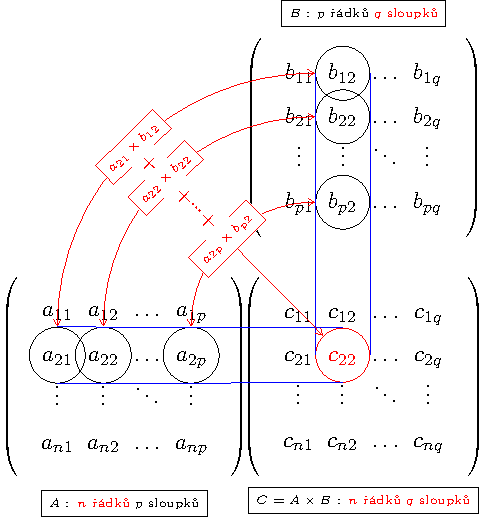
\includegraphics[width=0.45\linewidth]{mai_fig023a}}               &
        \subfloat[2. krok]{\label{LA:fig_LA001b}
          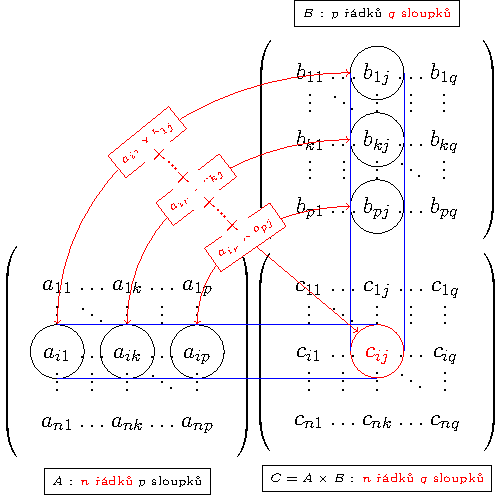
\includegraphics[width=0.45\linewidth]{mai_fig023b}} 
      \end{tabular}
      \caption{Postup při maticovém násobení}
    \end{figure}
  

      
      \begin{definition}\label{rovnost_matic}
       (Rovnost matic):  Matice \(\matr{A} = \left(a_{ij}\right)\) je rovna matici \(\matr{B}=
       \left(b_{kl}\right)\), jsou-li matice stejného typu a stejnolehlé prvky se sobě
       \textbf{rovnají}, tj. \(\matr{A} \in \mathbb{R}_{m,n}, \matr{B}\in\mathbb{R}_{m,n}, 
       a_{ij} = b_{ij}, \forall i\in\lbrace1,2,\ldots,m\rbrace, \forall j\in\lbrace1,2, \ldots 
       ,n\rbrace\).
      \end{definition}
      
%--------------------------------------------------------------------------------------------------
  \section{Počítání s vektory}\label{mai:IchapIIsecIV}
    \textbf{Vektory} budeme nazývat matice typu \(1/n\) a značit je
    \begin{equation*}
      \vec{u} = (u_1, u_2, \ldots, u_n).
    \end{equation*}
    Takže počítat s nimi již umíme! (V zápisu složek vektoru je vynechán řádkový index. V případě 
    matice s jedním řádkem, takzvané \emph{řádkové matice}, je totiž zbytečný.) Číslům \(u_1\) až 
    \(u_n\) budeme pro tuto chvíli říkat \emph{složky vektoru} \(\vec{u}\). Za chvíli tento pojem 
    ještě upřesníme. Celou řadu pojmů, s nimiž jsme se seznámili při počítání s maticemi, můžeme 
    pro vektory přímo použít. Namísto značení \(\mathcal{M} (1/n)\) budeme pro prostor vektorů 
    používat symbol \((\mathbb{R}^n)\) nebo \(\mathbb{C}^n\) (obvyklý symbol pro množinu 
    uspořádaných \(n\)-tic reálných nebo komplexních čísel).
    
    \subsection{Součiny vektorů}
      Kromě základních operací s vektory, tj. sčítání vektorů a násobení vektoru skalárem, se 
      často používají další operace, které obohacují \emph{strukturu vektorového prostoru}. 
      Zůstaneme u vektorů v trojrozměrném prostoru \(\mathbb{R}^3\) a definujeme si skalární, 
      vektorový a smíšený součin vektorů. Skalární součin vektorů definujeme prostřednictvím 
      geometrické definice jako zobrazení, které uspořádané dvojici vektorů (volných vektorů nebo 
      jejich libovolných umístění) přiřazuje reálný číslo podle předpisu
      \begin{equation}\label{mai:eq038}
        \vec{u}\vec{v} = \abs{\vec{u}}\cdot\abs{\vec{v}}\cos\varphi,
      \end{equation}
      kde \(\varphi = \sphericalangle(\vec{u},\vec{v})\) je velikost minimálního z obou úhlů mezi 
      vektory\(\vec{u},\vec{v}\).

    %---------------------------------------------------------------
    % !TeX spellcheck = cs_CZ
% \wikitextrule
\begin{mdframed}[style=mdexam]
  \begin{example}\label{mai:exam034}
    Vypočteme z definice \ref{mai:eq038} skalární součiny vektorů ortonormální báze \(\vec{e_1}\), 
    \(\vec{e_2}\) a \(\vec{e_3}\), spjaté s kartézskou soustavou souřadnic. Připomeňme, že tyto 
    vektory jsou jednotkové a navzájem kolmé.
    \begin{itemize}
      \item pro \(i\neq j\) \(\vec{e_i}\vec{e_j}=0\), 
                \(\sphericalangle\vec{e_i}\vec{e_j} =\dfrac{\pi}{2}\), vektory jsou kolmé,
      \item pro \(i = j\) \(\vec{e_i}\vec{e_j}=0\), 
                \(\sphericalangle\vec{e_i}\vec{e_j} =0, \abs{\vec{e_i}}=1\), vektory jsou 
                jednotkové.
    \end{itemize}

    Pro skalární součiny vektorů ortonormální báze použijeme zkrácené značení
    \begin{equation}\label{mai:eq085}
      \vec{e_i}\vec{e_j} = \delta_{ij},
    \end{equation}
    kde \(\delta_{ij}\) nabývá hodnoty \num{1} pro \(i = j\) a hodnoty \num{0} pro \(i \neq j\). 
    Nazývá se \textbf{Kroneckerovo delta} \cite[s.~40]{Musilova2009MA1}.
  \end{example}
\end{mdframed}
    %---------------------------------------------------------------
    
    Shrneme nyní vlastnosti skalárního součinu. Dokázat bychom je mohli, i když by to mohlo být i 
    velmi pracné, užitím znalostí z goniometrie. Zkuste to alespoň pro jednu z nich! Třeba se    
    vám podaří zvolit si tu nejjednodušší.

%} % tikzset
%---------------------------------------------------------------------------------------------------
\printbibliography[title={Seznam literatury}, heading=subbibliography]
\addcontentsline{toc}{section}{Seznam literatury}
%------------------- Differential calculus --------------------------------------------------------
  % !TeX spellcheck = cs_CZ
% Differential calculus
%{\tikzset{external/prefix={tikz/MAI/}}
% \tikzset{external/figure name/.add={ch03_}{}}
%---------------------------------------------------------------------------------------------------
% Limits_of_Functions.tex
%---------------------------------------------------------------------------------------------------
\chapter{Limita a spojitost funkce}\label{mai:IchapLimit}
\minitoc

  %================Podkapitola: Reálná funkce ======================================================
  \section{Reálná funkce}
    %-----------------------------------------------------------------------------------------------
    \small
    S funkcemi se setkáváme na každém kroku nejen ve fyzice a v ostatních přírodních vědách, ale i 
    v každodenním životě. Každá situace, kdy jsou nějaký jev či veličina jednoznačně a nevyhnutelně 
    určeny jinými jevy či veličinami, se dá popsat pomocí funkce\footnote{V matematice abstrahujeme 
    při zkoumání funkcionálních závislostí od konkrétní fyzikální povahy proměnných veličin a 
    chápeme je jako \uv{bezrozměrné veličiny}, tedy jako číselné proměnné. Někdy je jednoduché 
    takovou} funkci sestavit. Snadno například můžeme zjistit, jakou dráhu urazí automobil jedoucí 
    známou rychlostí v závislosti na tom, jak dlouho jede. Nebo dokážeme určit přírůstek našich 
    úspor ve spořitelně v závislosti na době spoření, pokud známe úrokovou míru a její změny. Jindy 
    je naopak skoro nemožné přijít na to, jak taková funkce vypadá, neboť nemáme dostatek informací 
    o parametrech, které do jejího zápisu vstupují. Třeba takovou závislost teploty ovzduší v daném 
    okamžiku na zeměpisné poloze a nadmořské výšce, kterou bychom si mohli představit jako jednu ze 
    samozřejmých součástí předpovědi počasí, bychom asi nesestavili. Popis jevů pomocí funkcí je v 
    každém případě velmi užitečný. Má však svá pravidla, s nimiž se v této kapitole seznámíme. 
    Závisí-li zkoumaný jev nebo veličina na jediné veličině, jejíž hodnoty jsou reálné a buď se 
    mění známým způsobem, nebo si je můžeme dokonce volit, hovoříme o \textbf{funkci jedné reálné 
    proměnné}. A lze-li zkoumaný jev nebo veličinu kvantifikovat rovněž pomocí reálných hodnot, 
    jedná se o \textbf{reálnou funkci jedné reálné proměnné}. Právě o takových funkcích bude v této 
    kapitole řeč. V aplikacích se budeme věnovat především funkcím, které mají význam ve fyzice a v 
    přírodních vědách. Velmi často půjde o funkce, kde reálnou proměnnou je čas. Jevy v přírodě 
    podléhají totiž principu příčinnosti, a tak lze velké množství veličin popisujících přírodní 
    jevy vyjádřit na základě znalosti přírodních zákonů jako funkce času. 
    \cite[s.~53]{Musilova2009MA1}
    \normalsize
    \subsection{Funkce a její graf}\label{MAI:section_002}
      V tomto odstavci se naučíme funkce zadávat, počítat s nimi a vyjádřit je velmi přehledným 
      způsobem — jejich \emph{grafem}. Zopakujme, že každou \textbf{reálnou funkci}, jejíž 
      definiční obor je podmnožina množiny \(\realset\), nazýváme \textbf{reálnou funkcí jedné 
      reálné proměnné}\footnote{Místo názvu \uv{reálná funkce jedné reálné proměnné} budeme pro 
      stručnost používat pouze název \uv{funkce}, pokud nebude řečeno něco jiného}.
      
      Protože \emph{funkce je speciální případ zobrazení}, můžeme všech\-ny pojmy a obecné 
      vlastnosti zobrazení přenést i na funkce. Některé z nich však vzhledem k důležitosti 
      zopakujme, případně doplníme. Na druhé straně budeme studovat také ty vlastnosti, které jsou 
      specifické pro tento speciální druh zobrazení.
      
      \begin{note}
        Je-li \(\mathcal{D}_f = \naturalset\), jedná se o \textbf{posloupnost}. (Speciálním 
        případem reálných funkcí jedné reálné proměnné jsou \emph{posloupnosti reálných čísel)}.
      \end{note}
      
      \subsection{Způsoby zadání funkce}\label{MAI:section_000}
        Nejprve funkci definujeme. Předpokládejme, že reálná proměnná, na níž bude záviset náš jev, 
        má dovoleno nabývat hodnot z určité předem stanovené podmnožiny \(D\subseteq\realset\) 
        reálných čísel. Předpokládejme dále, že podle určitého pravidla, předpisu, dokážeme pro 
        \emph{každou hodnotu} \(x\) množiny \(\mathcal{D}_f\), tj. \(x \in \mathcal{D}_f\), určit 
        \emph{právě jednu} reálnou hodnotu \(y\). Každé hodnotě \(x \in D\) tedy nějaké \(y\) 
        příslušet \emph{musí},  avšak žádné hodnotě \(x\) \emph{nesmíme} přiřadit více hodnot 
        \(y\). Tak vzniká funkce \(f\). Hodnoty \(x\) se nazývají hodnotami \emph{nezávisle 
        proměnné} (neboli \emph{argumentu}), hodnoty \(y\) hodnotami \emph{závisle proměnné} a 
        \(f\) symbolizuje \emph{funkční předpis}. Píšeme
        \begin{equation}\label{mai:eq000}
            f: x \in \mathcal{D}_f \rightarrow y=f(x)\in\realset
        \end{equation}
      Hodnoty proměnné \(x\) nazýváme též \emph{vzory}, odpovídající hodnoty \(y = f(x)\) 
      \emph{obrazy}. Množina  \(\mathcal{D}_f\) je \emph{definičním oborem} funkce \(f\). Zadání 
      definičního oboru je důležitou součástí zadání funkce. Množina \(H\) všech takových reálných 
      hodnot \(y\), které jsou obrazem nějakého vzoru, 
      \begin{equation}\label{mai:eq001}
          \mathcal{H}_f = 
              \left\lbrace 
                y\in\realset\text{ existuje } x\in \mathcal{D}_f, \text{ tak že } y = f(x)  
              \right\rbrace, 
      \end{equation}
      se nazývá \emph{obor hodnot} funkce \(f\). Hodnotu \(f(x)\) nazýváme také \emph{funkční 
      hodnotou} funkce \(f\) v bodě \(x\). 

      \begin{figure}[ht!] %\ref{mai:fig001}
        \centering
%        % Funkce jako „černá skříňka“. \cite[s.~54]{Musilova2009MA1}

\documentclass[11pt]{standalone}
\usepackage{xltxtra}
\usepackage{tikz}
\usepackage{amsmath}

\begin{document}
  \begin{tikzpicture}[fill=black!20]
%  \draw[help lines] (-1,-2) grid (6,3);
    \path (0,0) node(a) [ ] {\(\mathcal{D}_f\)}
    (2,0) node(b) [rectangle,rotate=0,draw,fill] {\(\begin{array}{c} \text{funkce} \\ f(x)  
    \end{array}\)}
    (4,0) node(c) [ ] {\(\mathcal{H}_f\)};
    \draw[thick,->] (a.east) -- (b);
    \draw[thick,->] (b.east) -- (c);
    \path [ ] (a.east) -- (b.west)   node [above,midway] {\(x\)};
    \path [ ] (b.east) -- (c.west)   node [above,midway] {\(y\)};
  \end{tikzpicture}

\end{document}
        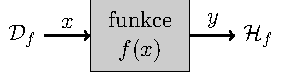
\includegraphics[width=0.45\linewidth]{mai_fig001.pdf}
        \caption{Funkce jako „černá skříňka“. \cite[s.~54]{Musilova2009MA1}}
        \label{mai:fig001}
      \end{figure}
      
      Funkci si podle obrázku \ref{mai:fig001} můžeme představit jako „černou skříňku“, do které 
      vstoupí hodnota (vzor) a vystoupí z ní hodnota \(y = f(x)\) (obraz). Množinu uspořádaných 
      dvojic čísel \([x, f(x)]\) nazveme \hyperref[MAI:section_001]{grafem funkce}.
      
      Jak zadat předpis \(f\)? Lze to udělat kterýmkoli z následujících způsobů, podle vhodnosti
      nebo snadnosti. Ukážeme jednotlivé možnosti na jednoduchém příkladu, kdy chceme hodnotám 
      proměnné \(x\) z množiny \(\mathcal{D}_f\) přiřadit jejich druhé mocniny. Zvolme pro náš 
      příklad definiční obor výčtem:
      \begin{equation*}
         \mathcal{D}_f = \lbrace-3,2,-1,0,1,2,3,4\rbrace,
      \end{equation*}
      a zadáme předpis
      \begin{itemize}\addtolength{\itemsep}{-0.5\baselineskip}
        \item \textbf{slovním popisem}: předpis \(f\) přiřazuje každé z hodnot \(x\in 
              \mathcal{D}_f\) její druhou mocninu,
        \item \textbf{vzorcem}: \(y = x^2\) pro \(x\in \mathcal{D}_f\) zadává zobrazení
              \begin{equation*}
                f: x\in \mathcal{D}_f \rightarrow f(x)= x^2\in\realset,
              \end{equation*}
        \item \textbf{tabulkou}: Hodnoty obrazů pro všechny vzory z \(\mathcal{D}_f\) vypíšeme do 
              tabulky:
              \begin{table}[h]
                \centering
                \begin{tabular}{c|rrrrrrrr}
                  \textbf{x} & -3 & -2 & -1 & 0 & 1 & 2 & 3 & 4  \\ \hline
                  \textbf{y} & 9  & 4  & 1  & 0 & 1 & 4 & 9 & 16
                \end{tabular}
                % \caption{ }
              \end{table}
              Proměnná $x$ se v tomto případě mění \uv{diskrétně}. Je zřejmé, že tímto způsobem 
              můžeme funkci definovat úplně jen tehdy, je-li definiční obor konečná množina. 
              Tabulku však používáme i v jiných případech, zejména chceme-li vyznačit pomocí ní, 
              některé hodnoty, které nás z nějakého důvodu přednostně zajímají. 
        \item Zadání \textbf{grafem}: 
          \begin{equation*}
            G_f = \left\lbrace\left[x,f(x)\right] |x\in D\right\rbrace
                = \left\lbrace\left[x,x^2 \right] |x\in D\right\rbrace
          \end{equation*}
          tak, že dvojice \([x, f(x)]\) znázorníme jako body v rovině (obr. \ref{MAI:fig_011}).
          \begin{figure}[ht!]
            \centering  
            \begin{tabular}{cc}
              \subfloat[ ]{\label{MAI:fig_011}
                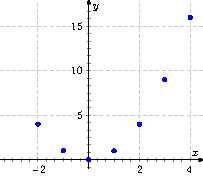
\includegraphics[width=0.4\linewidth]{mai_fig002.pdf}}              &
              \subfloat[ ]{\label{MAI:fig_010}
                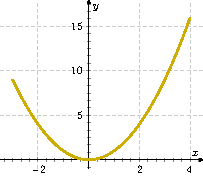
\includegraphics[width=0.4\linewidth]{mai_fig003.pdf}}              \\
            \end{tabular}
            \caption{Zadání funkce grafem}
          \end{figure}
          Z grafu můžeme ovšem funkční hodnoty určit pouze přibližně. Pro další matematické 
          zpracování je grafické zadání nejméně vhodné, i když jeho praktický význam například v 
          technických aplikacích nelze popřít.
        \item Zadání pomocí \textbf{rovnice}, jíž je funkce řešením: některé funkce nelze jednoduše 
              zapsat pomocí některého z předchozích způsobů, nebo to alespoň nejde přesně. Lze však 
              zapsat (diferenciální) rovnici, kterou tato funkce splňuje. Jedná se většinou o 
              speciální funkce, jimž se v tomto textu nebudeme věnovat. (Někdy může být taková 
              rovnice  představující zadání funkce i velmi jednoduchá. Například dosti známá funkce 
              \(\erf(x)\), \emph{error funkce}, velmi úzce souvisí s funkcí \(f(x) = 
              \frac{2}{\sqrt{x}}e^{-x^2}\). Nelze ji však zapsat vzorcem. Některé její hodnoty v 
              nejčastěji používaném rozsahu proměnné \(x\) můžeme najít v rozsáhlých tabulkách, 
              které byly sestaveny pomocí numerických metod.)
      \end{itemize}
      
      Již bylo zmíněno, že zadání definičního oboru je neopominutelnou součástí zadání funkce. 
      Kdybychom například zadali funkci opět předpisem \(y=x^2\), avšak za definiční obor stanovili 
      uzavřený interval \(D = \lbrace —3,4\rbrace\), dostali bychom graf na obrázku 
      \ref{MAI:fig_010}. Jde skutečně o jinou funkci než na obrázku \ref{MAI:fig_011}. Její úplnou 
      tabulku bychom nedokázali napsat vůbec.
      
%      Nejčastější způsob zadání funkce představuje \emph{vzorec}. Tabulku alespoň pro některé 
%      hodnoty z \(\mathcal{D}_f\) si pak dokážeme sestavit a schematický graf nakreslit. Někdy se 
%      objeví zadání funkce jen v podobě vzorce, například: „Je dána funkce \(y = f(x)\).“ Znamená 
%      to, že autor zapomněl zadat definiční obor? Nemusí tomu tak být. Tento způsob zadání chápeme 
%      tak, že si sami musíme stanovit „co největší“ definiční obor této funkce, tj. určit množinu 
%      všech takových \(x\), pro která lze do vzorce dosadit a hodnotu \(y\) určit.

      Zobrazovací předpis, kterým je funkce zadána, může být rozmanitý. Nejčastěji a pro účely 
      matematické analýzy nejvhodnější je \emph{analytické zadání vzorcem}, tj. rovnicí tvaru 
      $y=f(x)$ nebo několika takovými rovnicemi platnými pro různé části definičního oboru. Přitom 
      v rovnici $y=f(x)$ je na pravé straně nějaký správně definovaný výraz obsahující nejvýše 
      proměnnou $x$ a nabývající jednoznačné hodnoty pro danou hodnotu proměnné $x$.
      
%      Někdy však používáme (poněkud nedůsledně) termíny \uv{funkce \(f(x)\)} nebo \uv{funkce 
%      \(y=f(x)\)}. V tomto smyslu nepojímáme již \(x\) jako pevný prvek z definičního oboru, ale 
%      jako \uv{nezávisle proměnnou} neboli \emph{argument}, tj. symbol zastupující libovolný prvek 
%      z definičního oboru. V tomto případě pak písmeno \(y\) v rovnici \(y=f(x)\) nazýváme 
%      \emph{závisle proměnnou} a říkáme, že \uv{\(y\) závisí na \(x\)}. Tato frazeologie má své 
%      historické kořeny; tento způsob vyjádření funkce budeme využívat zřídka, zejména tam, kde 
%      nechceme pro označení příslušné funkce zavádět zvláštní symbol. Tak např. budeme mluvit o 
%      funkci \(e^x\) (ačkoliv se zavádí pro exponenciální funkci symbol exp) nebo o funkci \(\sin 
%      x\) (ačkoliv by bylo důslednější mluvit o funkci \(\sin\)) apod. \cite[s.~82]{Brabec1989} 

    %-------------------------------------
      % !TeX spellcheck = cs_CZ
\begin{mdframed}[style=mdexam]
  \begin{example}\label{MAI:exam017}
    (Definiční obor a obor hodnot funkce): Určíme „co největší“ definiční obor funkce
    \(y=\log_2{(\sqrt{1-x^2})}\) a zjistíme také její obor hodnot.
        
    {\centering
    \captionsetup{type=figure}
  %   % !TeX spellcheck = cs_CZ
% exam017.tex
% K příkladu \ref{fyz:fey_exam017} \(y=\log_2{(\sqrt{1-x^2})}\) 

\documentclass[11pt]{standalone}
\usepackage{xltxtra}
\usepackage[usenames,x11names]{xcolor}
\usepackage{tikz}
\usepackage{pgfplots}
  \pgfplotsset{compat=newest}
\usepackage{amsmath}

\begin{document}
  \begin{tikzpicture}[thick,scale=0.7, every node/.style={transform shape}]
    \begin{axis}[
      xmin = -1, xmax = 1, ymin = -10, ymax = 0,
      domain = -0.999999:0.999999,
      restrict y to domain=-30:0,
      grid = major,   % both
      grid style={line width=.1pt, draw=gray!20},
      major grid style={dashed, line width=.2pt, draw=gray!40},
      minor tick num=5,
      clip = true,
      clip mode=individual,
      axis x line = middle,
      axis y line = middle,
      xlabel={\(x\)},
    %  xlabel style={at=(current axis.right of origin), anchor=west},
      ylabel={\(y\)},
    %  ylabel style={at=(current axis.above origin), anchor=south},
      enlarge y limits={rel=0.13},
      enlarge x limits={rel=0.07},
    ]
    
     \addplot[color=Gold3, samples=1000, smooth, ultra thick, unbounded coords=jump, no markers] 
        gnuplot{log10(sqrt(1-x^2))/log10(2)};  
    \end{axis}
  \end{tikzpicture}

\end{document}

% note: předchozí varianta MAI013
%\begin{tikzpicture}
%    \begin{axis}[
%        axis lines=middle,
%        width=10cm, height=10cm,     % size of the image
%        grid = both,
%        grid style={dashed, gray!30},
%        enlargelimits=true,
%        xmin=-1,      % start the diagram at this x-coordinate
%        xmax= 1,      % end   the diagram at this x-coordinate
%        ymin= -6,     % start the diagram at this y-coordinate
%        ymax= 0.5,     % end   the diagram at this y-coordinate
%        /pgfplots/xtick={-1,-0.5,...,1},   % make steps of length 0.2
%        /pgfplots/ytick={0,-0.5,...,-6},   % make steps of length 0.1
%        axis background/.style={fill=white},
%        axis line style={thick, shorten >=2pt, ->, > = {Latex[scale=1.3]}},
% %       every axis x label/.style={
% %        at={(ticklabel* cs:1.0)},
% %        anchor=west,
% %       },
% %       every axis y label/.style={
% %        at={(ticklabel* cs:1.0)},
% %        anchor=south,
% %       },
%        every axis x label/.style={at={(current axis.right of origin)},anchor=west},
%        every axis y label/.style={at={(current axis.north)},above=0mm},
%        ylabel=\(y\),
%        xlabel=\(x\),
% %       title={Dirichletova funkce}
%      ]
%      \addplot[domain=-0.9999:0.9999, line width=0.5pt,samples=1000,red]{log2(sqrt(1-x^2))};
%    \end{axis} 
%\end{tikzpicture}
    \luafigure[0.9]{mai_fig004.pdf}
    \captionof{figure}{K příkladu \ref{MAI:exam017} \(y=\log_2{(\sqrt{1-x^2})}\) 
    \cite[s.~57]{Musilova2009MA1}
    \label{mai:fig004}}
    \par}
    
    Využijeme našich znalostí ze střední školy. Ve hře jsou tři funkce: logaritmus, odmocnina a
    kvadratická funkce, postupně: 
    \begin{equation*}
      y = \log_2w, \qquad w = \sqrt{u}, \qquad u = 1 - x^2.
    \end{equation*}
    „Největším“ definičním oborem logaritmu je množina \(\mathcal{D}(log) = {w\realset \mid w >
    0}\). Oborem hodnot logaritmu pro \(w \in \mathcal{D}(log)\) je celá reálná osa. Hodnoty \(w\)
    však dostáváme vyčíslením odmocniny, která pro přípustné hodnoty \(u\), \(\mathcal{D}(\sqrt{ })
    = \lbrace u\in\realset \lvert u\geq 0\rbrace\), může nabývat všech nezáporných hodnot, tj.
    kladných a hodnoty nula (té nabývá pro \(u = 0\)). Hodnotu \(w = 0\) však nesmíme do logaritmu
    dosadit, takže hodnotu \(u = 0\) musíme ihned vyloučit. Hodnoty proměnné \(x\) musíme omezit
    tak, aby kvadratická funkce \(u = 1 - x^2\) nabývala pouze kladných hodnot. Dostáváme tak
    definiční obor funkce \(y = f(x)\) \(\mathcal{D}=\lbrace x\in\realset \lvert -1<x<1\rbrace\),
    neboli otevřený interval \((-1, 1)\). Pro \(x \in \mathcal{D}\) pak funkce \(u(x)\) nabývá
    hodnot v intervalu \(\mathcal{H}_u = \left( 0, 1\right]\) a funkce \(\log_2\sqrt{1-x^2}\) hodnot
    v intervalu \(\mathcal{H}_u = \left( -\infty, 0\right]\), který je tedy jejím oborem hodnot.
    Graf funkce vidíme na obr. \ref{mai:fig004}. 
  \end{example}
\end{mdframed}
    %-----------------------------------------------------------------------------------------------
    \subsection{Graf funkce}\label{MAI:section_001}\hypertarget{MAI:section_001}
      Jinými slovy, v předchozím odstavci, bylo řečeno, že každé funkci můžeme přiřadit její graf, 
      a že \textbf{grafem funkce} $f:A\rightarrow\realset,\ A\subset\realset$, rozumíme množinu 
      všech bodů euklidovské roviny, jejíž souřadnice $x$, $y$ v dané kartézské soustavě souřadnic 
      vyhovuje rovnice 
      \begin{equation}\label{mai:eq026}
        y=f(x). 
      \end{equation}  
      
      Graf funkce může v jednodušších případech posloužit jako prostředek k získání názorné 
      \uv{představy}. Grafy některých funkcí jsou \uv{křivky}, (intuitivním smyslu tohoto slova). 
      Avšak u některých funkcí názorná představa grafu selhává. Vezmeme-li např. Dirichletovu 
      funkci, snadno zjistíme, že její graf nemůžeme sestrojit (obr. \ref{mai:fig005} tedy 
      není grafem funkce, ale pouze pokusem o názorné přiblížení Dirichletovi funkce)
      
      \begin{figure}[ht!] %\ref{mai:fig005}
        \centering
%       % !TeX spellcheck = cs_CZ
%
% Pokus o zobrazení Dirichletovy funkce: \uv{dvě rovnoběžné přímky $y=0$ a $y=1$ s 
% nekonečným množstvím mezer}
% xelatex -enable-write18 -shell-escape mai_fig005.tex

\documentclass[11pt]{standalone}
\usepackage{xltxtra}
\usepackage[usenames,x11names]{xcolor}
\usepackage{tikz}
\usepackage{pgfplots}
  \pgfplotsset{compat=newest}
\usepackage{amsmath}
\usepackage{amsfonts}           % \mathbb{Q}
\usepackage{tabularx}           % \shortstack

\begin{document}
  \begin{tikzpicture}[thick,scale=0.7, every node/.style={transform shape}]
    \begin{axis}[
      xmin = -3, xmax = 3, ymin = 0, ymax = 2,  % osy
      domain = -3:3,
      restrict y to domain=0:4,
      grid = major,   % both
      grid style={line width=.1pt, draw=gray!20},
      major grid style={dashed, line width=.2pt, draw=gray!40},
      minor tick num=5,
      clip = true,
      clip mode=individual,
      axis x line = middle,
      axis y line = middle,
      xlabel={\(x\)},
    %  xlabel style={at=(current axis.right of origin), anchor=west},
      ylabel={\(y\)},
    %  ylabel style={at=(current axis.above origin), anchor=south},
      enlarge y limits={rel=0.13},
      enlarge x limits={rel=0.07},
    %  title={Dirichletova funkce}
    ]
        
        \addplot[domain=-3:3, ultra thick,samples=10,blue] {1};
        \label{plot one}
        \addplot[domain=-3:3, ultra thick,samples=10,red] {0};
        \label{plot two} 
        \node [draw,fill=white] at (rel axis cs: 0.6,0.7) {\shortstack[l]{
        \(f(x) = 
          \left\lbrace\begin{array}{l@{}l@{}}
              1 & \text{ když } x \in  \mathbb{Q}\\
              0 & \text{ když } x \in  \mathbb{R} \setminus\mathbb{Q}
          \end{array}\right.
       \)
          }
           };
      \end{axis} 
  \end{tikzpicture}
\end{document}
        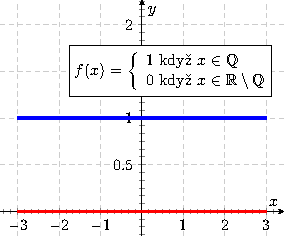
\includegraphics[width=0.5\linewidth]{mai_fig005.pdf}
        \caption{Pokus o zobrazení Dirichletovy funkce: \uv{dvě rovnoběžné přímky $y=0$ a $y=1$ s 
        nekonečným množstvím mezer}}
        \label{mai:fig005}
      \end{figure}      
      Z předchozí kapitoly také víme, že zadat funkci znamená udat její definiční obor a 
      \uv{zobrazovací předpis}, tj pravidlo (formulované slovně či v používaném matematickém 
      jazyku), podle něhož můžeme jednoznačným způsobem rozhodnout, jaká funkční hodnota odpovídá 
      libovolně zvolenému číslu z definičního oboru. Definičním oborem bývá často interval nebo 
      sjednocení intervalů. Není-li definiční obor udán, rozumíme jím množinu všech reálných čísel, 
      pro něž je příslušný předpis definován. Tuto množinu nazýváme \textbf{přirozeným} (též 
      maximálním) definičním oborem funkce. Je to tzv. \emph{existenční obor} výrazu, jímž je 
      funkce definována \cite[s.~84]{Brabec1989}.
      
      Například funkce $f: \realset\rightarrow\realset,\ f(x)=x^2$, můžeme vyjádřit bez udání 
      definičního oboru $\realset$ vztahem 
      \begin{equation*}
        f: y=x^2,
      \end{equation*}
      neboť předpis $y=x^2$ má smysl pro každé reálné číslo $x$. Avšak u funkce $g:\langle0, 
      1\rangle\rightarrow\realset,\ g(x)=x^2,$ je nutné v zápisu funkce definiční obor $\langle0, 
      1\rangle$ 
      uvést, píšeme tedy   
      \begin{equation*}
        g: y=x^2, \quad x\in\langle0,1\rangle.
      \end{equation*}
       
      %-------------------------------------
        % !TeX spellcheck = cs_CZ
\wikitextrule
\begin{example}\label{MAI:exam018} 
  Vzorcem $f(x)=\sqrt{1-x}$ je dána funkce, jejímž přirozeným oborem je interval 
  $(-\infty,1\rangle$ (uvažme, že výraz $\sqrt{1-x}$ je definován v reálném oboru, je-li 
  $1-x\geq0$). Graf této funkce je část paraboly, jejíž osou je osa $x$, viz obr. 
  \ref{mai:fig006}.
  
  {\centering
   \captionsetup{type=figure}
%  % !TeX spellcheck = cs_CZ
% mai_fig006.tex

\documentclass[11pt]{standalone}
\usepackage{xltxtra}
\usepackage[usenames,x11names]{xcolor}
\usepackage{tikz}
\usepackage{pgfplots}
  \pgfplotsset{compat=newest}
\usepackage{amsmath}


\begin{document}
  \begin{tikzpicture}[thick,scale=0.7, every node/.style={transform shape}]
    \begin{axis}[
      xmin = -3, xmax = 1.5, ymin = 0, ymax = 3,  % osy
      domain = -3:1,
      restrict y to domain=0:4,
      grid = major,   % both
      grid style={line width=.1pt, draw=gray!20},
      major grid style={dashed, line width=.2pt, draw=gray!40},
      minor tick num=5,
      clip = true,
      clip mode=individual,
      axis x line = middle,
      axis y line = middle,
      xlabel={\(x\)},
    %  xlabel style={at=(current axis.right of origin), anchor=west},
      ylabel={\(y\)},
    %  ylabel style={at=(current axis.above origin), anchor=south},
      enlarge y limits={rel=0.13},
      enlarge x limits={rel=0.07},
    ]
    
     \addplot[color=Gold3, samples=200, smooth, ultra thick, unbounded coords=jump, no markers] 
        gnuplot{sqrt(1-x)};  
    \end{axis}
  \end{tikzpicture}
\end{document} 
   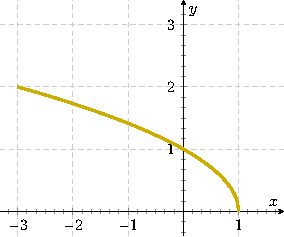
\includegraphics[width=0.5\linewidth]{mai_fig006.pdf}
   \captionof{figure}{{Graf funkce $y=\sqrt{1-x}$ je část paraboly, jejíž hlavní osou je osa $x$}}
   \label{mai:fig006}
   \par}

\end{example}
      %-------------------------------------
      
      %-------------------------------------
        % !TeX spellcheck = cs_CZ
\begin{mdframed}[style=mdexam]
  \begin{example}\label{MAI:exam019} 
    Funkce je dána vzorcem 
    \begin{equation*}
      f(x):y=\abs{x}.
    \end{equation*} 
    Přirozeným definičním oborem této funkce je množina $\realset$. Táž funkce může být dána i 
    vzorcem
    \begin{equation*}
      f(x):y=\sqrt{x^2},
    \end{equation*}    
    nebo dvěma rovnicemi
    \begin{equation*}
      f(x):y=
        \begin{cases}
             x & \text{je-li} x \geq 0. \\
            -x & \text{je-li} x < 0,
        \end{cases}                 
    \end{equation*}  
    což je zřejmé, uvědomíme-li si jak je definována absolutní hodnota. Graf funkce je na obr. 
    \ref{mai:fig007}.
    
    {\centering
    \captionsetup{type=figure}
  %  % !TeX spellcheck = cs_CZ
% mai_fig007.tex

\documentclass[11pt]{standalone}
\usepackage{xltxtra}
\usepackage[usenames,x11names]{xcolor}
\usepackage{tikz}
\usepackage{pgfplots}
  \pgfplotsset{compat=newest}
\usepackage{amsmath}

\begin{document}
  \begin{tikzpicture}[thick,scale=0.7, every node/.style={transform shape}]
    \begin{axis}[
      xmin = -3, xmax = 3, ymin = 0, ymax = 3,  % osy
      domain = -3:3,
      restrict y to domain=0:3,
      grid = major,   % both
      grid style={line width=.1pt, draw=gray!20},
      major grid style={dashed, line width=.2pt, draw=gray!40},
      minor tick num=5,
      clip = true,
      clip mode=individual,
      axis x line = middle,
      axis y line = middle,
      xlabel={\(x\)},
    %  xlabel style={at=(current axis.right of origin), anchor=west},
      ylabel={\(y\)},
    %  ylabel style={at=(current axis.above origin), anchor=south},
      enlarge y limits={rel=0.13},
      enlarge x limits={rel=0.07},
    ]
    
     \addplot[color=Gold3, samples=200, smooth, ultra thick, unbounded coords=jump, no markers] 
        gnuplot{abs(x)};  
    \end{axis}
  \end{tikzpicture} 
\end{document}
    \luafigure[0.9]{mai_fig007.pdf}
    \captionof{figure}{Graf funkce $y=\abs{x}$}
    \label{mai:fig007}
    \par}
  \end{example}
\end{mdframed}
      %-------------------------------------
      
      Funkce může být analyticky zadána i jinak než vzorcem $y=f(x)$. Časté je \textbf{parametrické 
      vyjadřování}, tj. vyjádření dvojicí rovnic 
      \begin{equation}\label{mai:eq027}
        x=\varphi(t),\ y=\psi(t),\ t\in J,
      \end{equation}
      kde $\varphi, \psi$ jsou funkce definované na množině $J$ ($\ J$ bývá obvykle interval). 
      Proměnná $t$ se nazývá \emph{parametr}: má zde pomocný význam. Zajímá nás totiž vztah mezi 
      $x$ a $y$. Rovnice \ref{mai:eq027} definuje relaci 
      $f\subset\realset\times\realset=\realset^2$:
      \begin{equation*}
        f = \{(x,y)\in\realset^2; \text{ existuje } t\in J \text{ tak, že } x=\varphi(t),\ y=\psi(t)\}.
      \end{equation*}      
      Tato relace může být za \emph{určitých podmínek jednoznačná} tj. je funkcí z $\realset$ do 
      $\realset$. V tomto případě říkáme, že funkce $f$ je \emph{definována parametricky rovnicemi 
      \ref{mai:eq027}}
      
      %-------------------------------------
        % !TeX spellcheck = cs_CZ
\begin{mdframed}[style=mdexam]
  \begin{example}\label{mai:exam020} 
    Rovnice $x=\cos t,\ y=\sin t\quad t\in\langle0,\pi\rangle$, definují parametricky funkci 
    \begin{equation}
      f: y= \sqrt{1-x^2}, \quad x\in\langle-1,1\rangle,
    \end{equation}
    jejíž grafem je polokružnice, ležící v horní polorovině $\{(x,y)\in\realset^2, y\geq0\}$.
    
    {\centering
    \captionsetup{type=figure}
  %   % !TeX spellcheck = cs_CZ
%Graf funkce \(y=\sqrt{1-x^2}\) je polokružnice

\documentclass[11pt]{standalone}
\usepackage{xltxtra}
\usepackage[usenames,x11names]{xcolor}
\usepackage{tikz}
\usepackage{pgfplots}
  \pgfplotsset{compat=newest}
\usepackage{amsmath}

\begin{document}
  \begin{tikzpicture}[thick,scale=0.7, every node/.style={transform shape}]
    \begin{axis}[
      xmin = -1.2, xmax = 1.2, ymin = 0, ymax = 1.3,  % osy
      domain = -1:1,
      restrict y to domain=0:1,
      unit vector ratio=1 1 1,  % axis equal
      grid = major,   % both
      grid style={line width=.1pt, draw=gray!20},
      major grid style={dashed, line width=.2pt, draw=gray!40},
      minor tick num=5,
      clip = true,
      clip mode=individual,
      axis x line = middle,
      axis y line = middle,
      xlabel={\(x\)}, ylabel={\(y\)},
      enlarge y limits={rel=0.07},
      enlarge x limits={rel=0.07},
    ]
    
      \addplot[color=Gold3, samples=200, smooth, ultra thick, unbounded coords=jump, no markers] 
         gnuplot{sqrt(1-x^2)};  
    \end{axis}
  \end{tikzpicture} 
\end{document}
    \luafigure[0.9]{mai_fig008.pdf}
    \captionof{figure}{Graf funkce \(y=\sqrt{1-x^2}\) je polokružnice}
    \label{mai:fig008}
    \par}
  \end{example}
\end{mdframed}
      %-------------------------------------
      
      Blíže se parametrickým zadáním funkce budeme zabývat v kapitole \ref{chap:Apl_dif_poc}
      (Aplikace diferenciálního počtu).
      
      Funkce může být někdy zadána též rovnicí tvaru 
      \begin{equation}\label{mai:eq028}
        F(x,y) = 0.
      \end{equation}
      Přitom $F$ je funkce dvou proměnných, tj. zobrazení z $\realset^2\rightarrow\realset$. Kromě 
      rovnice \ref{mai:eq028} může být dána ještě podmínka, aby bod $(x,y)$ patřil k některé 
      množině $M\subset\realset^2$. Rovnicí \ref{mai:eq028} je definována opět jakási relace 
      $f\subset\realset\times\realset$,
      \begin{equation}
        f = \{(x,y)\in\realset^2,\quad F(x,y)=0 \}
      \end{equation}
      (případně $f = \{(x,y)\in\realset^2,\ F(x,y)=0,\ (x,y)\in M \}$), zajímá nás, kdy tato relace 
      je funkcí z $\realset$ do $\realset$. Říkáme pak, že funkce $f$ je dána \textbf{implicitně} 
      uvedenou rovnicí \ref{mai:eq028} (příp. rovnicí \ref{mai:eq028} a podmínkou $(x,y)\in 
      M$). Naproti tomu zadání funkce ve tvaru $y=f(x)$ nazýváme \textbf{explicitním}.

      %-------------------------------------
        % !TeX spellcheck = cs_CZ
\begin{mdframed}[style=mdexam]
  \begin{example}\label{MAI:exam022}\todo[inline]{Nedokončený příklad}
    \begin{itemize}
    \item[]
    \item  Rovnicí $x+2y-3=0$ je implicitně definována funkce  
          $f:y=-\dfrac{1}{2}x+\dfrac{3}{2}$.
    \item  Rovnicí $x^2+y^2=1$ a podmínkou $y\geq0$ je definována implicitní funkce z příkladu 
          \ref{MAI:exam020}. Relace $\{(x,y)\in\realset^2;\ x^2+y^2=1\}$ není ovšem jednoznačná, 
          každé hodnotě $x\in(-1,1)$ odpovídají dvě hodnoty $y: y_1=\sqrt{1-x^2}$, $y: y_2 = 
          -\sqrt{1-x^2}$. Podmínkou $y\geq0$ druhou hodnotu vylučujeme. Místo podmínky $y\geq0$ 
          bychom mohli uvést i jiné podmínky, aby rovnice $x^2+y^2=1$ určovala implicitní funkci.   
    \end{itemize}
  \end{example}
\end{mdframed}
      %-------------------------------------
      
      Vyšetřování podmínek, při nichž rovnice $F(x,y)=0$ je definována funkce $f$, se obvykle 
      provádí metodami matematické analýzy funkce více proměnných. 
          
    %---------------------------------------------------------------------------------------------- 
    \subsection{Vlastnosti funkcí}\label{MA1:subsec_vlastnosti_funkce}
      \subsubsection{Omezená funkce}
        \begin{definition}\label{MA1:def_lim01}
          Funkci $f$ nazýváme shora (zdola) omezenou na množině $A\subset D(f)$, je-li shora 
          (zdola) omezená množina funkčních hodnot $f(A)$. Je-li funkce $f$ omezená shora i zdola 
          na množině $A$, pak ji nazýváme omezenou na množině $A$. Je-li $A=D(f)$, nazýváme funkci 
          omezenou. Viz kniha \cite[s.~87]{Brabec1989}       
        \end{definition}
        Funkce \(f\) je omezená na množině \(A\), právě když existuje číslo \(K>0\) tak, že platí
        \begin{align*}
         |f(x)|      &\leq K \qquad \text{pro každé } x\in A   \\ 
         \shortintertext{neboli}
         -K\leq f(x) &\leq K \qquad \text{pro každé } x\in A. 
        \end{align*}

        %-------------------------------------
          % !TeX spellcheck = cs_CZ
\wikitextrule
\begin{example}\label{MAI:exam023}
  Funkce $f:y=\dfrac{1}{x^2+1}$ je omezená. Platí totiž 
  \begin{equation*}
    \left|\frac{1}{x^2+1}\right|=\frac{1}{x^2+1}\leq1 \qquad \text{pro všechna }x\in\realset.
  \end{equation*}
  Zdola je tato funkce omezena dokonce číslem $0$.  
\end{example}
        %-------------------------------------

        \begin{itemize}\addtolength{\itemsep}{-0.5\baselineskip}
          \item Je-li funkce $f$ shora omezená na množině $A$, existuje konečné \emph{supremum}     
                $\sup f(A)$. Toto číslo nazýváme \emph{supremem funkce $f$ na množině $A$} a 
                označujeme je též $\sup_{x\in A}f(A)$ nebo $\sup\{f(x), x\in A\}$.
          \item Je-li funkce $f$ zdola omezená na množině $A$, existuje konečné \emph{infimum} 
                $\inf(A)$, které nazýváme \emph{infimum funkce $f$ na množině $A$} a označujeme je 
                též $\inf_{x\in A}f(A)$ nebo $\inf\{f(x), x\in A\}$. 
          \item Není-li funkce $f$ shora (zdola) omezená na množině $A$, pak je ovšem $\sup_{x\in A}
                f(x)=+\infty$ ($\sup_{x\in A} f(x)=-\infty$).
          \item Má-li množina $f(A)$ největší (nejmenší) prvek, pak toto číslo nazýváme největší 
                (nejmenší hodnotou funkce $f$  na množině $A$ (je-li $A = f(f)$, též absolutním 
                maximem, resp. absolutním minimem funkce $f$) a značíme je $\max_{x\in A} f(x)$ 
                ($\min_{x\in A} f(x)$). V tomto případě existuje takové číslo $x_0\in A$, že 
                $f(x_0)=\max_{x\in A}f(x)$ ($f(x_0)=\min_{x\in A}f(x)$). Pro všechna $x\in A$ tedy 
                platí $f(x)\leq f(x_0)$ ($f(x)\geq f(x_0)$). Je zřejmé, že největší (nejmenší) 
                hodnota funkce $f$ na množině $A$, pokud existuje je současně supremem (infimem) 
                funkce $f$ na $A$.
        \end{itemize}

      %-------------------------------------
        % !TeX spellcheck = cs_CZ
\wikitextrule
\begin{example}\label{MAI:exam021} 
  Pro funkci z příkladu \ref{MAI:exam023} platí:
  \begin{align*}
    \sup_{x\in\realset}&=\frac{1}{x^2+1}=\max_{x\in\realset}=\frac{1}{x^2+1}=1;   \\
    \inf_{x\in\realset}&=\frac{1}{x^2+1}=0,
  \end{align*}
  tato funkce však nenabývá v definičním oboru $\realset$ nejmenší hodnoty, neboť je stále 
  $\dfrac{1}{x^2+1}>0$. To, že infimum je $0$, dokážeme takto: Zvolíme-li libovolně 
  $\varepsilon>0$, pak snadno zjistíme, že existuje $x$, pro něž 
  $\dfrac{1}{x^2+1}<\varepsilon$:
  \begin{align*}
    1                  &< \varepsilon(x^2+1) \\
    \frac{1}{\epsilon} &< x^2+1 \Rightarrow \sqrt{\frac{1}{\epsilon}-1} < x
  \end{align*} 
  
  {\centering
   \captionsetup{type=figure}
%   % !TeX spellcheck = cs_CZ
%Graf funkce $f(x):y=\dfrac{1}{1+x^2}$

\documentclass[11pt]{standalone}
\usepackage{xltxtra}
\usepackage[usenames,x11names]{xcolor}
\usepackage{tikz}
\usepackage{pgfplots}
  \pgfplotsset{compat=newest}
\usepackage{amsmath}

\begin{document}
  \begin{tikzpicture}[thick,scale=0.7, every node/.style={transform shape}]
    \begin{axis}[
      xmin = -4.2, xmax = 4.5, ymin = 0, ymax = 1.3,  % osy
      domain = -4:4,
      restrict y to domain=0:1,
  %    unit vector ratio=1 1 1,  % axis equal
      grid = major,   % both
      grid style={line width=.1pt, draw=gray!20},
      major grid style={dashed, line width=.2pt, draw=gray!40},
      minor tick num=5,
      clip = true,
      clip mode=individual,
  %    /pgfplots/xtick={-2,-1,1,2}, % make steps of length 0.2
      axis x line = middle,
      axis y line = middle,
      xlabel={\(x\)}, ylabel={\(y\)},
      enlarge y limits={rel=0.07},
      enlarge x limits={rel=0.07},
    ]
    
      \addplot[color=Gold3, samples=200, smooth, ultra thick, unbounded coords=jump, no markers] 
         gnuplot{1/sqrt(1+x^2)};  
    \end{axis}
  \end{tikzpicture}
\end{document} 
   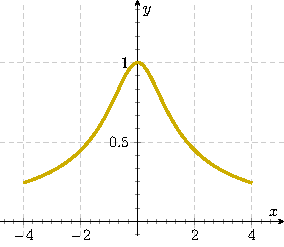
\includegraphics[width=0.5\linewidth]{mai_fig009.pdf}
   \captionof{figure}{Graf funkce $f(x):y=\dfrac{1}{1+x^2}$}
   \label{mai_fig009}
  \par}
  
  Neexistuje tedy kladné číslo, jež by bylo dolní mezí množiny funkčních hodnot, takže infimum je 
  $0$. Graf funkce $f$ je na obr. \ref{mai_fig009}.
\end{example}
      %-------------------------------------
       
      \subsubsection{Monotonní funkce}
        \begin{definition}\label{MA1:def_lim02}
          Funkci $f$ nazýváme \textbf{rostoucí (klesající)} na množině $A\subset D(f)$, jestliže 
          pro každé dva body $x_1, x_2\in A,\ x_1<x_2$, platí $f(x_1)<f(x_2)$ ($f(x_1)>f(x_2)$). 
          Funkci $f$ nazýváme \textbf{neklesající (nerostoucí)} na množině $A\subset D(f)$, 
          jestliže pro každé dvě body $x_1, x_2\in A,x_1<x_2$, platí $f(x_1)\leq f(x_2)$ 
          ($f(x_1)\geq f(x_2)$). Rostoucí a klesající funkce (na množině $A$) se nazývají 
          \textbf{ryze monotónní} (na množině $A$), neklesající a nerostoucí funkce (na množině 
          $A$) se nazývají monotónní (na množině $A$).    
        \end{definition}
            
        Z definice je zřejmé, že každá rostoucí funkce je zároveň neklesající a každá klesající 
        funkce je zároveň nerostoucí. Ryze monotónní funkce tvoří tedy podmnožinu množiny 
        monotónních funkcí. 
           
        \begin{example}
          Funkce $y=2x+1$ je \textbf{rostoucí} na intervalu $(-\infty, \infty)$. Platí totiž: $x_1<x_2\Rightarrow 2x_1<2x_2\Rightarrow2x_1+1<2x_2+1$.
        \end{example}
        \begin{example}
          Funkce y=[x] je \textbf{neklesající} na intervalu $(-\infty, \infty)$ (viz příklad **). 
        \end{example}
        \begin{example}
          Heavisideova funkce (viz příklad **) je \textbf{neklesající} na intervalu $(-\infty, \infty)$ (viz příklad **). 
        \end{example}       
        \begin{example}
          Funkce $y=|x|$ je \textbf{klesající} na intervalu $(-\infty, 0\rangle$ a rostoucí na intervalu $\langle0, \infty)$. 
        \end{example}  
            
        \begin{definition}\label{MA1:def_lim03}
          Funkci $f$ nazýváme \textbf{konstantní} na množině $A$, jestliže pro každé dva body $x_1, 
          x_2\in A$, platí $f(x_1)=f(x_2)$. V tom případě existuje reálné číslo $k$ takové, že pro 
          každé $x\in A$ je $f(x)=k$. Je-li $k=0$, mluvíme o nulové funkci na množině $A$. 
        \end{definition} 
          
        Výrok \uv{funkce $f$ je konstantní na množině $A$} zapisujeme též $f(x)=\text{konst na }A$. 
        Funkci konstantní na $\realset$ budeme stručně nazývat \textbf{konstantní funkcí} nebo 
        krátce \textbf{konstantou}. Z textu bude obvykle patrno, interpretujeme-li symbol $k$ jako 
        reálné číslo nebo jako konstantní funkci. Je zřejmé, že konstantní funkce na množině $A$ je 
        zároveň neklesající i nerostoucí na množině $A$. Toto tvrzení se dá obrátit. Lze snadno 
        dokázat i tuto větu:        
        \begin{lemma}\label{MA1:lem_lim01}
          Funkce $f$ je \textbf{rostoucí} na množině $A$, právě když je neklesající na množině $A$ a na žádné dvoubodové podmnožině $B\subset A$ není konstantní. 
        \end{lemma}
        Obdobná tvrzení platí i pro klesající funkce. 
               
      \subsubsection{Sudé a liché funkce}
        \begin{definition}\label{MA1:def_lim04}
          Funkce $f$ se nazývá \textbf{sudá} jestliže pro každé $x\in D(f)$ je též $-x\in D(f)$  a 
          platí $f(x)=f(-x)$.
          Funkce $f$ se nazývá \textbf{lichá} jestliže pro každé $x\in D(f)$ je též $-x\in D(f)$  a 
          platí $f(-x)=-f(x)$. 
        \end{definition}
        Graf sudé funkce je souměrný podle osy $y$ (osy funkčních hodnot), graf liché funkce je  
        souměrný podle počátku. 
 
       %-------------------------------------
         % !TeX spellcheck = cs_CZ
\wikitextrule
\begin{example}\label{MAI:exam024} 
  Funkce $f:\,y=x^2$ je sudá, funkce $g:\,y=x^3$ je lichá.
  
  {\centering
   \begin{tabular}{cc}
     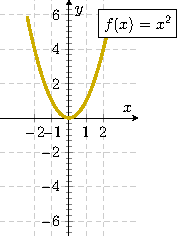
\includegraphics[width=0.5\linewidth]{mai_fig010.pdf}              &
     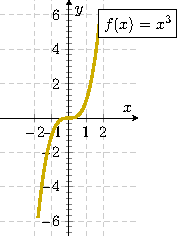
\includegraphics[width=0.5\linewidth]{mai_fig011.pdf}             \\
  \end{tabular}
  \captionsetup{type=figure}
  \captionof{figure}{Příklad sudé a liché funkce}\label{MAI:fig_002}
  \par}
\end{example}
       %-------------------------------------

        Daná funkce nemusí být ovšem ani sudá, ani lichá. Snadno se dokáže tvrzení:
        \begin{itemize}
          \item Je-li sudá funkce $f$ na množině $D(f)\cap\langle0,\infty)$ rostoucí (klesající),
                je na množině $D(f)\cap(-\infty,0\rangle$ klesající (rostoucí).
          \item Je-li lichá funkce na množině $D(f)\cap\langle0,\infty)$ rostoucí (klesající),
                je též na množině $D(f)\cap(-\infty,0\rangle$ klesající (rostoucí).                 
        \end{itemize}
      \subsubsection{Periodická funkce}

    \subsection{Operace s funkcemi. Uspořádání}
      Jak s funkcemi počítat? Definujeme základní operace s nimi — \emph{součet funkcí, součin 
      funkcí a násobení funkce reálným číslem}. Předpokládejme, že na definičním oboru 
      \(\mathcal{D}\) jsou zadány funkce \(f\) a \(g\) a reálné číslo \(\alpha\). Pak na tomtéž 
      definičním oboru lze zadat nové funkce
      \begin{align*}
        \mathcal{F} &: \mathcal{D}\ni x\,\rightarrow\,\mathcal{F}(x) = f(x)+g(x)  \in\realset   \\
        \mathcal{G} &: \mathcal{D}\ni x\,\rightarrow\,\mathcal{G}(x) = \alpha g(x)\in\realset   \\
        \mathcal{H} &: \mathcal{D}\ni x\,\rightarrow\,\mathcal{H}(x) = f(x) g(x)  \in\realset 
      \end{align*}
      Funkce \(\mathcal{F}\), \(\mathcal{G}\) a \(\mathcal{H}\) nazýváme postupně součtem funkcí 
      \(f\) a \(g\), \(\alpha\)-násobkem funkce \(f\) a součinem funkcí \(f\) a \(g\). Značíme
      \begin{equation*}
       \mathcal{F} = f + g, \qquad \mathcal{G} = \alpha f, \qquad \mathcal{H} = fg. 
      \end{equation*}
      
      Všimněme si nyní pravidel pro počítání s funkcemi zadanými na \(\mathcal{D}\) a zjistíme, 
      že se velmi podobají pravidlům pro počítání s reálnými čísly. Není divu, vždyť operace s 
      funkcemi jsou definovány prostřednictvím funkčních hodnot, a těmi jsou reálná čísla. Některé 
      důležité odlišnosti však přece jen najdeme. Napřed ale pravidla:
      
      \begin{itemize}\addtolength{\itemsep}{-0.5\baselineskip}
        \item komutativní zákon pro součet funkcí
          \begin{equation}\label{mai:eq012}
            f(x) + g(x) = g(x) + f(x)
          \end{equation}
        \item asociativní zákon pro součet funkcí  
          \begin{equation}\label{mai:eq013}
            (f(x) + g(x)) + h(x) = f(x) + (g(x) + h(x)
          \end{equation}
        \item existence univerzálního neutrálního  prvku \(O\) (nulová funkce \(O:\mathcal{D}\ni x 
          \rightarrow O(x)=0\))
          \begin{equation}\label{mai:eq014}
            f(x) + O = O + f(x) = f(x)
          \end{equation}
        \item existence právě jednoho opačného prvku k funkci \(f\), přičemž \((-f)(x) = -f(x)\)
          \begin{equation}\label{mai:eq015}
            f(x)+(-f(x))=(-f(x))+f(x)=O
          \end{equation}
        \item asociativní zákon pro násobení číslem 
         \begin{equation}\label{mai:eq016}
            (\alpha_1\alpha_2)f(x) = \alpha_1(\alpha_2f(x))
         \end{equation}
        \item  1. distributivní zákon pro násobení číslem
          \begin{equation}\label{mai:eq017}
            \alpha(f(x)+g(x) =\alpha f(x) + \alpha g(x)
          \end{equation}\label{mai:eq018}
        \item 2. distributivní zákon pro násobení číslem 
          \begin{equation}\label{mai:eq019}
            (\alpha_1+\alpha_2)f(x) =\alpha_1f(x)+\alpha_2f(x)
          \end{equation}
        \item násobení číslem \((—1)\) dává opačný prvek
          \begin{equation}\label{mai:eq020}
            (-1)f(x)=(-f(x))
          \end{equation}
        \item komutativní zákon pro součin funkcí
          \begin{equation}\label{mai:eq021}
            f(x)g(x)=g(x)f(x)
          \end{equation}
        \item asociativní zákon pro součin funkcí 
          \begin{equation}\label{mai:eq022}
            f(x)(g(x)h(x))=(f(x)g(x))h(x)
          \end{equation}
        \item distributivní zákon zprava pro součin funkcí
          \begin{equation}\label{mai:eq023}
            (f_1(x) + f_2(x))g(x) =f_1(x)g(x) + f_2(x)g(x)
          \end{equation}
        \item distributivní zákon zleva pro součin funkcí
          \begin{equation}\label{mai:eq024}
            f(x)(g_1(x) + g_2(x))=f(x)g_1(x)+f(x)g_2(x)
          \end{equation}
        \item násobení jednotkovou funkcí \(I: \mathcal{D}\ni x \rightarrow I(x) = 1\)  
          \begin{equation}\label{mai:eq025}
           f(x)I=If(x)
          \end{equation}
        \item existence právě jedné \emph{převrácené} funkce k funkci \(f\) pro \(f(x)\neq0\quad 
              (f)^{-1}: \bar{D}\ni x\rightarrow (f)^{-1}(x)=[f(x)]^{-1}\) kde \(\bar{\mathcal{D}} 
              = \mathcal{D} - \left\{x\in \mathcal{D}\,|\,f(x)=0\right\}\)
          \begin{equation}
            f(x)(f(x))^{-1}=(f(x))^{-1}f(x) = I
          \end{equation}
      \end{itemize}
      Všimněme si, že funkce \((f)^{-1}\) existuje obecně na užším definičním oboru 
      \(\bar{\mathcal{D}}\), než na kterém je definována funkce \(f\). Je totiž třeba vyloučit 
      všechny hodnoty \(x\), pro které \(f(x) = 0\) (zákaz dělení nulou). K funkci \(O\) tedy 
      převrácená funkce neexistuje vůbec!
      
      Existence opačné a převrácené funkce k \(f\) umožňuje definovat \emph{rozdíl} a \emph{podíl} 
      funkcí \(f-g=f+(-g)\) a \(\dfrac{f}{g}=f(g)^{-1}\), tj.
      \begin{align*}
        f-g         &: \mathcal{D}\ni x\,\rightarrow\, (f-g)(x)=f(x)+(-g)(x)= f(x)-g(x), \\
        \frac{f}{g} &: \bar{D}\ni x\,\rightarrow\, 
                       \left(\frac{f}{g}\right)(x) = f(g)^{-1}(x) = \frac{f(x)}{g(x)}, 
      \end{align*}
      kde \(\bar{D}=D-\left\{x\in D\,|\,g(x)=0 \right\}\) 
      
      \begin{note}
        Pamatujme si označení převrácené funkce jako \((f)^{-1}\), v němž je zápis symbolu \(f\) do 
        závorky podstatný. Jde o něco jiného než znamená symbol \(f^{-1}\) bez závorky, který 
        rezervujeme pro inverzní funkci v dalším výkladu.
      \end{note}
      \begin{note}
        Porovnáme-li nyní vlastnosti operací s funkcemi a pravidla pro počítání s reálným čísly, 
        komplexními čísly, maticemi a vektory, můžeme konstatovat, že množina funkcí s operací 
        sčítání funkcí a násobení funkce číslem je \textbf{vektorovým prostorem}. To je vlastnost, 
        která je s případem čísel, matic a vektorů společná. Vektorový prostor funkcí se však od 
        zmiňovaných vektorových prostorů výrazně liší svou dimenzí (rozměrem). Intuitivně dobře 
        chápeme, co znamená jednorozměrný, dvojrozměrný a trojrozměrný prostor (například 
        \(\realset^1\), \(\realset^2\), \(\realset^3\)). V odstav 1.4 jsme dokonce pracovali v 
        n-rozměrném vektorovém prostoru. Dimenze vektorového prostoru může být i nekonečná — třeba 
        zrovna u funkcí. Obecně jde o pojem poměrně obtížný a budeme se jím důkladně zabývat až v 
        kapitolách věnovaných algebře \cite[s.~58]{Musilova2009MA1}.
      \end{note}
      
      Operace s funkcemi jsme definovali a prodiskutovali pro případ, kdy definiční obory funkcí, 
      vstupujících do operace byly stejné. Co když tomu tak nebude? Znamená to, že pak nemůžeme 
      funkce sčítat, násobit, apod.? Předpokládejme, že definičním oborem funkce \(f\) je množina 
      \(\mathcal{D}_f\) definičním oborem funkce \(g\) množina \(D_g\). Pokud jsou tyto obory 
      disjunktní, tj. \(\mathcal{D}_f \cap \mathcal{D}_g = 0\), můžeme utvořit pouze 
      \(\alpha\)-násobek funkce \(f\) či \(g\). Sčítat ani násobit funkce \(f\) a \(g\) nemůžeme 
      neboť hodnota \(f(x) + g(x)\) ani \(f(x)g(x)\) neexistuje pro žádné \(x\). Pokud je průnik 
      \(D=d_f\cap D_g\) oborů \(\mathcal{D}_f\) a \(\mathcal{D}_g\) neprázdný, stává se definičním 
      oborem funkcí \(f+g\) a \(fg\). Platí stejná pravidla jako v předchozí tabulce, pouze s 
      omezením na obor \(\mathcal{D}_f\).
    
    \subsection{Skládání a inverze funkcí}
      \emph{Skládání} neboli kompozici funkcí si lze snadno představit opět pomocí „černých 
      skříněk“ (obr. \ref{mai:fig012}): Do první skřínky představující předpis \(g\), \emph{vnitřní 
      složku} složené funkce, vstupuje
      \begin{figure}[ht!] %\ref{mai:fig012}
        \centering
%        % !TeX spellcheck = cs_CZ
% exam017.tex

\documentclass[11pt]{standalone}
\usepackage{xltxtra}
\usepackage[usenames,x11names]{xcolor}
\usepackage{tikz}
\usepackage{pgfplots}
  \pgfplotsset{compat=newest}
\usepackage{amsmath}
\usepackage{amsfonts}          % \mathbb{R}
  \newcommand{\realset}{\mathbb{R}}

\begin{document}
  \begin{tikzpicture}[fill=black!20]
  %  \draw[help lines] (-1,-2) grid (6,3);
    \path (0,0) node(a) [ ] {\(\mathcal{D}_g\)}
    (2,0) node(b) [rectangle,rotate=0,draw,fill] 
      {\(\begin{array}{c} \text{funkce} \\ g  \end{array}\)}
    (4.5,0) node(c) [rectangle,rotate=0,draw,fill] 
      {\(\begin{array}{c} \text{funkce} \\ f  \end{array}\)}
    (7,0) node(d) [ ] {\(\realset\)};
    \draw[thick,->] (a.east) -- (b);
    \draw[thick,->] (b.east) -- (c);
    \draw[thick,->] (c.east) -- (d);
    \path [ ] (a.east) -- (b.west)   node [above,midway] {\(x\)};
    \path [ ] (b.east) -- (c.west)   node [above,midway] {\(g(x)\)};
    \path [ ] (c.east) -- (d.west)   node [above,midway] {\(f[g(x)]\)};
  \end{tikzpicture}
\end{document}
        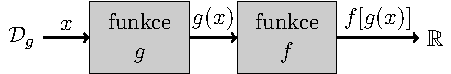
\includegraphics[width=0.45\linewidth]{mai_fig012.pdf}
        \caption{Skládání funkcí \cite[s.~59]{Musilova2009MA1}}
        \label{mai:fig012}
      \end{figure}
      hodnota \(x\) z definičního oboru \(\mathcal{D}_g\) funkce \(g\). Výstupem je číslo \(u = 
      g(x)\), funkční hodnota vnitřní složky v bodě \(x\). Toto číslo smí vstoupit do skříňky 
      představující předpis \(f\), \emph{vnější složku} složené funkce, právě tehdy, je-li prvkem 
      jejího definičního oboru \(\mathcal{D}_f\). V takovém případě najdeme na výstupu ze skříňky 
      \(f\) hodnotu \(y = f(u) = f[g(x)]\). (Jestliže \(g(x)\notin\mathcal{D}_f\), není výstup ze 
      skříňky \(f\) definován.) Vzniká nový předpis \(F\), kterým se některým bodům definičního 
      oboru \(\mathcal{D}_g\), ne všem, ale pouze těm, pro něž \(g(x)\in\mathcal{D}_f\), 
      přiřazují hodnoty \(f[g(x)]\). Definujme nyní složenou funkci přesněji: Předpokládejme, že 
      jsou zadány funkce
      \begin{align*}
        g  &: \mathcal{D}_g\ni x\,\rightarrow\, g(x) = u\in\realset, \\
        f  &: \mathcal{D}_f\ni u\,\rightarrow\, f(u) = y\in\realset. \\
        \shortintertext{označme}
        \mathcal{D} &= \{x|x\in\mathcal{D}_g \text{ a současně } g(x)\in\mathcal{D}_f\}.
      \end{align*}
      Pokud \(\mathcal{D} = \emptyset\), lze definovat funkci
      \begin{equation*}
        F: \mathcal{D}\ni x\rightarrow y = F(x) = f[g(x)]\in\realset, 
           \text{ značíme } F = f \circ g.
      \end{equation*}
      \(F\) se nazývá \emph{složením} neboli \emph{kompozicí} funkcí \(g\) a \(f\). Zápis \(f\circ 
      g\) čteme často také jako \emph{„f po g“}. Skládat lze i větší počet funkcí.

       %-------------------------------------
         % !TeX spellcheck = cs_CZ
\begin{mdframed}[style=mdexam]
  \begin{example}\label{MAI:exam025}
    Uvažme funkci z příkladu \ref{vol02:fyz:fey_exam017}. 
    
    {\centering
    \captionsetup{type=figure}
  %   % !TeX spellcheck = cs_CZ
\documentclass[11pt]{standalone}
\usepackage{xltxtra}
\usepackage[usenames,x11names]{xcolor}
\usepackage{tikz}
\usepackage{pgfplots}
  \pgfplotsset{compat=newest}
\usepackage{amsmath}

\begin{document}
  \begin{tikzpicture}[thick,scale=0.7, every node/.style={transform shape}]
    \begin{axis}[
      xmin = -5, xmax = 5, ymin = -10, ymax = 1.5,
   %   domain = -0.999999:0.999999,
      restrict y to domain=-30:1.5,
      unit vector ratio=1 1 1,  % axis equal
      grid = both,   % both, major
      grid style={line width=.1pt, draw=gray!20},
      major grid style={dashed, line width=.2pt, draw=gray!40},
      minor tick num=4,
      clip = true,
      clip mode=individual,
      axis x line = middle,
      axis y line = middle,
      xlabel={$x$},
    %  xlabel style={at=(current axis.right of origin), anchor=west},
      ylabel={$u,w,y$},
    %  ylabel style={at=(current axis.above origin), anchor=south},
      enlarge y limits={rel=0.13},
      enlarge x limits={rel=0.07},
    ]
    
      \addplot[color=Gold3, samples=1000, smooth, ultra thick, unbounded coords=jump, no markers, 
               domain = -0.999999:0.999999] 
        gnuplot{log10(sqrt(1-x^2))/log10(2)};  
        
     \addplot[color=green, samples=200, smooth, ultra thick, unbounded coords=jump, no markers, 
     domain = -3.3:3.3] 
        gnuplot{1-x^2};
        
     \addplot[color=blue, samples=200, smooth, ultra thick, unbounded coords=jump, no markers, 
     domain = -1:1] 
        gnuplot{sqrt(1-x^2)};  
    \end{axis}
  \end{tikzpicture}
\end{document}
    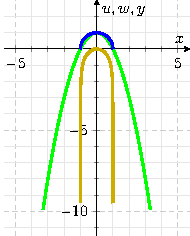
\includegraphics[width=0.6\linewidth]{mai_fig013.pdf}
    \captionof{figure}{K příkladu \ref{MAI:exam025} \(y=\log_2{(\sqrt{1-x^2})}\) 
    \cite[s.~57]{Musilova2009MA1}
    \label{mai:fig013}}
    \par}
    
    Ukážeme, jak tato funkce vzniká postupně složením tří funkcí a jak při tom dochází k postupnému 
    omezování definičního oboru. Písmeny \(\mathcal{D}\) a \(H\) s příslušným indexem budeme značit 
    definiční obory a obory hodnot jednotlivých funkcí.
    \begin{gather*}
      \begin{align*}
        g&:  \realset =\mathcal{D}_g\ni x\rightarrow u=g(x) = 1- x^2  \in\mathcal{H}_g=(-\infty,1], \\
        h&: [0,\infty)=\mathcal{D}_h\ni u\rightarrow w=h(u) = \sqrt{u}\in\mathcal{H}_h=[0,\infty),  \\
       \shortintertext{\(\mathcal{D}_h\cap\mathcal{H}_g = [0,1]\Rightarrow\mathcal{D}_{h\circ g}=[-1,1], 
                       \mathcal{H}_{h\circ g} = [0,1],\)}                                    \\
       f&:(0,\infty)=\mathcal{D}_f\ni w \rightarrow y=f(w)=\log_2w\in\mathcal{H}_f=\realset  \\
       \shortintertext{\(\mathcal{H}_{h\circ g}\cap\mathcal{D}_f = (0,1] 
                       \Rightarrow\mathcal{D}_F=(-1,1),\mathcal{H}_F=(-\infty,0].\)} 
      \end{align*}
    \end{gather*}
    Je tedy
    \begin{gather*}
      \begin{align*}
        F:\mathcal{D}_F\ni x\rightarrow 
        y&=F(x)=(f\circ(h\circ g))(x) = f{h[g(x)]}          \\
        &= \log_2\sqrt{1-x^2}\in(-\infty,0].
      \end{align*}
    \end{gather*}
    Názorněji než tento zápis ukazuje situaci obrázek \ref{mai:fig013}.
  \end{example}
\end{mdframed}
       %-------------------------------------
      
      Může vzniknout otázka, jak rozpoznáme vnitřní a vnější složku složené funkce. Rozlišit 
      vnitřní a vnější složku třeba u funkcí \(\cos(x^2)\) a \((cos x)^2\) není problém. Hned také 
      vidíme, že obecně \(f\circ g\neq g\circ f\), i když by definiční obory funkcí na pravé i levé 
      straně měly neprázdný průnik. Jsou však i případy na první pohled méně zřetelné, jak ukazuje 
      následující příklad.
      
      %-------------------------------------
        % !TeX spellcheck = cs_CZ
\begin{mdframed}[style=mdexam]
  \begin{example}\label{mai:exam026}
    (Určení vnitřní a vnější složky) Uveďme příklad dvou funkcí \(F(x)=\sqrt{x^2}\) a \(G(x) =
    (\sqrt{x})^2\). Liší se tyto funkce, nebo jde o tutéž funkci, jen jinak zapsanou? Vidíme, že
    platí

    \begin{align*}
      \mathcal{D}_F &=\realset, F(x)=\abs{x}\forall x\in\mathcal{D}_F, \mathcal{H}_F = [0, infty),\\
      \mathcal{D}_G &=[0, \infty), G(x)=x\forall    x\in\mathcal{D}_G, \mathcal{H}_G = [0, infty).
    \end{align*}
    Funkce \(F\) a \(G\) mají různé definiční obory, ale na jejich průniku dávají stejné funkční
    hodnoty. Ani zde však obecně nelze pořadí skládání funkcí zaměňovat.
  \end{example}
\end{mdframed}
      %-------------------------------------
       
      Funkce \(F\) a \(G\) mají různé definiční obory, ale na jejich průniku dávají stejné funkční 
      hodnoty. Ani zde však obecně nelze pořadí skládání funkcí zaměňovat.
      
      Nyní se pusťme do vybudování pojmu inverzní funkce k funkci \(f\). Představme si, že funkční
      hodnota \(y = f(x)\) zadané funkce
      \begin{equation*}
        f: \mathcal{D}_f\ni x \rightarrow f(x)\in\mathcal{H}_f
      \end{equation*}
      představuje „zakódovanou“ informaci o hodnotě \(x\). Položme si otázku, zda a za jakých 
      podmínek dokážeme sestavit „černou skříňku“, na jejímž výstupu by se při vstupu obrazu \(y = 
      f(x)\) objevila hodnota \(x\). Omezení takové možnosti je názorně vidět na obrázku 
      \ref{mai:fig014}. V případě funkce \(f(x)\) lze ke všem obrazům \(y \in \mathcal{H}_f\) najít 
      vzory, v případě funkce \(g(x)\) to možné není, neboť jeden a týž obraz lze získat z několika 
      vzorů. Pro který bychom se tedy měli rozhodnout?
      
      \begin{figure}[ht!] %\ref{mai:fig014}
        \centering
%        % !TeX spellcheck = cs_CZ
% Skládání funkcí \cite[s.~61]{Musilova2009MA1}

\documentclass[11pt]{standalone}
\usepackage{xltxtra}
\usepackage[usenames,x11names]{xcolor}
\usepackage{tikz}
\usepackage{pgfplots}
  \pgfplotsset{compat=newest}
\usepackage{amsmath}
\usepackage{amsfonts}       % \mathbb{R}
  \newcommand{\realset}{\mathbb{R}}

\begin{document}
  \begin{tikzpicture}[fill=black!20]
  %  \draw[help lines] (-1,-2) grid (6,3);
    \path (0,0) node(a) [ ] {\(\mathcal{D}_f\)}
    (2,0) node(b) [rectangle,rotate=0,draw,fill] 
      {\(\begin{array}{c} \text{funkce} \\ f  \end{array}\)}
    (4.5,0) node(c) [rectangle,rotate=0,draw,fill] 
      {\(\begin{array}{c} \text{funkce} \\ f^{-1}  \end{array}\)}
    (7,0) node(d) [ ] {\(\realset\)};
    \draw[thick,->] (a.east) -- (b);
    \draw[thick,->] (b.east) -- (c);
    \draw[thick,->] (c.east) -- (d);
    \path [ ] (a.east) -- (b.west)   node [above,midway] {\(x\)};
    \path [ ] (b.east) -- (c.west)   node [above,midway] {\(f(x)\)};
    \path [ ] (c.east) -- (d.west)   node [above,midway] {\(x\)};
  \end{tikzpicture}
\end{document}
        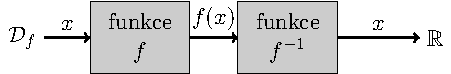
\includegraphics[width=0.45\linewidth]{mai_fig014.pdf}
        \caption{Skládání funkcí \cite[s.~61]{Musilova2009MA1}}
        \label{mai:fig014}
      \end{figure}
       Aby bylo možné vzor zpětně identifikovat na základě znalosti obrazu, je třeba, aby funkce 
       \(f\) byla \emph{prostá}, tj. aby předpis \(f\) přiřazoval každým dvěma různým vzorům \(X_1 
       \neq x_2\) dva různé obrazy \(f(x_1) \neq f(x_2)\). Často lze tohoto požadavku docílit tím, 
       že se místo funkce \(f\) s definičním oborem \(\mathcal{D}_f\) spokojíme s funkcí, která 
       vznikne omezením \emph{(restrikcí)} té původní na „menší“ definiční obor, zato však již bude 
       prostá. U funkce \(g\) na obrázku \ref{mai:fig016} by tak stačilo omezit definiční obor 
       například na množinu \(\mathcal{D}_g\). Než inverzní funkci definujeme, ukažme si způsob 
       jejího nalezení na známém příkladu.

       \begin{figure}[ht!]
         \centering  
         \begin{tabular}{cc}
           \subfloat[ ]{\label{mai:fig016a}
             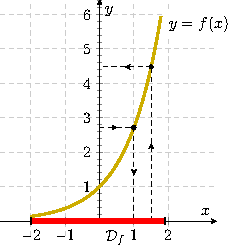
\includegraphics[width=0.45\linewidth]{mai_fig016a.pdf}}              &
           \subfloat[ ]{\label{mai:fig016b}
             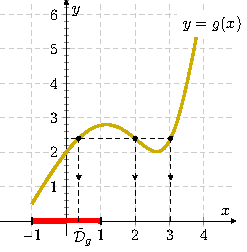
\includegraphics[width=0.45\linewidth]{mai_fig016b.pdf}}              \\
         \end{tabular}
         \caption{K pojmu inverzní funkce}
         \label{mai:fig016}
       \end{figure}
      
      %-------------------------------------
        % !TeX spellcheck = cs_CZ
\begin{mdframed}[style=mdexam]
  \begin{example}\label{MAI:exam027}
    (Nalezení inverzní funkce): Funkci 
    \begin{equation*}
      y = \log_2(\sqrt{1-x^2})
    \end{equation*}
    Jsme již z různých hledisek rozebrali v příkladech \ref{vol02:fyz:fey_exam017} a
    \ref{MAI:exam025}. Hodí se i nyní.

    {\centering
    \captionsetup{type=figure}
  %  % !TeX spellcheck = cs_CZ
% K příkladu \ref{mai:exam027} \(y=\log_2{(\sqrt{1-x^2})}

\documentclass[11pt]{standalone}
\usepackage{xltxtra}
\usepackage[usenames,x11names]{xcolor}
\usepackage{tikz}
\usepackage{pgfplots}
  \pgfplotsset{compat=newest}
\usepackage{amsmath}

\begin{document}
  \begin{tikzpicture}[thick,scale=0.7, every node/.style={transform shape}]
    \begin{axis}[
      xmin = -5, xmax = 5, ymin = -5, ymax = 1.5,
   %   domain = -0.999999:0.999999,
      restrict y to domain=-30:1.5,
      unit vector ratio=1 1 1,  % axis equal
      grid = both,   % both, major
      grid style={line width=.1pt, draw=gray!20},
      major grid style={dashed, line width=.2pt, draw=gray!40},
      minor tick num=4,
      clip = true,
      clip mode=individual,
      axis x line = middle,
      axis y line = middle,
      xlabel={\(x\)},
    %  xlabel style={at=(current axis.right of origin), anchor=west},
      ylabel={\(y\)},
    %  ylabel style={at=(current axis.above origin), anchor=south},
      enlarge y limits={rel=0.13},
      enlarge x limits={rel=0.07},
    ]
    
      \addplot[color=Gold3, samples=1000, smooth, ultra thick, unbounded coords=jump, no markers, 
               domain = 0:0.9995] 
        gnuplot{log10(sqrt(1-x^2))/log10(2)};  
        
      \addplot[color=blue, samples=200, smooth, ultra thick, unbounded coords=jump, no markers, 
               domain = -5:0] 
        gnuplot{sqrt(1-2^(2*x))};  
    \end{axis}
  \end{tikzpicture}
\end{document}
    \luafigure[0.9]{mai_fig015.pdf}
    \captionof{figure}{K příkladu \ref{MAI:exam027} \(y=\log_2{(\sqrt{1-x^2})}\) 
    \cite[s.~62]{Musilova2009MA1}
    \label{mai:fig015}}
    \par}
    
    Na obrázku \ref{mai:fig013} máme dokonce její graf, a tak vidíme, že \textbf{není} na svém 
    definičním oboru \((-1, 1)\) \textbf{prostá}. Omezme proto její definiční obor na interval 
    \(\mathcal{D} = [0, 1)\), na němž již prostá je (část grafu vpravo od osy \(y\)). Pro danou 
    hodnotu obrazu \(y \in (-\infty,0]\) můžeme již jednoznačně určit hodnotu \(x\) jednoduchou 
    úpravou:
    \begin{align*}
      y = \log_2(\sqrt{1-x^2}) &\Rightarrow \sqrt{1-x^2} = 2^y   \\
                               &\Rightarrow x^2 = 1 - 2^{2y}     \\
                               &\Rightarrow x = \sqrt{1 - 2^{2y}}
    \end{align*}
    Formální záměnou \(x \leftrightarrow y\) dostáváme inverzní funkci k funkci \(f\),
    \begin{equation*}
      y =f^{-1}(x) = \sqrt{1 - 2^{2x}}.
    \end{equation*}
    Grafy obou funkcí jsou na obrázku \ref{mai:fig015}.
  \end{example}
\end{mdframed}
      %-------------------------------------
      
      Ze způsobu konstrukce funkce \(f^{-1}\) v předchozím příkladu je vidět, že 
      \(\mathcal{D}_{f^{-1}} = \mathcal{H}_f\), \(\mathcal{H}_{f^{-1}} = \mathcal{D}_f\) a graf 
      inverzní funkce je obrazem grafu prosté funkce \(f\) při osové symetrii v rovině 
      souřadnicových os vzhledem k ose prvního a třetího kvadrantu. Nyní již definujeme inverzní 
      funkci obecně. Předpokládejme, že funkce \(f : \mathcal{D}_f\ni x \rightarrow y = f(x)\ni 
      \mathcal{H}_f\) je prostá na svém definičním oboru. Pak existuje funkce \(f^{-1}\) definovaná 
      jako
      \begin{equation}\label{mai:eq029}
        f^{-1} :\mathcal{H}_f\ni x\rightarrow y = f^{-1}(x)\in\mathcal{D}_f\Leftrightarrow x = f(y).
      \end{equation}
      Funkci \(f^{-1}\) nazýváme \textbf{inverzní funkcí k funkci} \(f\). Ještě shrneme pravidla 
      pro skládání funkcí a pro inverzní funkce:

      \begin{itemize}\addtolength{\itemsep}{-0.5\baselineskip}
        \item asociativní zákon pro skládání funkcí
          \begin{equation}\label{mai:eq030}
            f(x)\circ(h(x)\circ g(x)) = f(x)\circ h(x) \circ g(x)
          \end{equation}
        \item distributivní zákon zleva 
          \begin{equation}\label{mai:eq031}
            f(x) \circ (h(x) + g(x)) = f(x) \circ h(x) + f(x) \circ g(x)
          \end{equation}
        \item existence univerzálního neutrálního  prvku \(O\) (nulová funkce \(O:\mathcal{D}\ni x 
          \rightarrow O(x)=0\))
          \begin{equation}\label{mai:eq032}
            f(x) + O = O + f(x) = f(x)
          \end{equation}
        \item existence právě jednoho opačného prvku k funkci \(f\), přičemž \((-f)(x) = -f(x)\)
          \begin{equation}\label{mai:eq033}
            f(x)+(-f(x))=(-f(x))+f(x)=O
          \end{equation}
        \item komutativní zákon pro součet funkcí
          \begin{equation}\label{mai:eq034}
            f(x) + g(x) = g(x) + f(x)
          \end{equation}
        \item asociativní zákon pro součet funkcí  
          \begin{equation}\label{mai:eq035}
            (f(x) + g(x)+h(x) = f(x) + (g(x) + h(x)
          \end{equation}
        \item existence univerzálního neutrálního  prvku \(O\) (nulová funkce \(O:\mathcal{D}\ni x 
          \rightarrow O(x)=0\))
          \begin{equation}\label{mai:eq036}
            f(x) + O = O + f(x) = f(x)
          \end{equation}        
      \end{itemize}   
      Předchozí vztahy platí na patřičně zúžených definičních oborech funkcí, které do nich 
      vstupují.
      
  %-------------------------------------------------------------------------------------------------
  \section{Elementární funkce}
      Základními elementárními funkcemi nazýváme \cite[s.~10]{PolakMA1}:
%      \begin{displaymath}
%        \xymatrix{
%        \mbox{mocninné} & *+[F]{\mbox{Elementární 
%        funkce}}\ar@{->}[l]\ar@{->}[dl]\ar@{->}[d]\ar@{->}[dr]\ar@{->}[r]&\mbox{exponenciální} \\
%        \mbox{goniometrické}       &   \mbox{logaritmické}      & \mbox{cyklometrické}
%        }
%      \end{displaymath}
    %------------- Goniometrické funkce ------------------------------------------------------------
    \subsection{Goniometrické funkce}  
    \begin{itemize}
      \item \textbf{Základní vzorce pro goniometrické funkce}
        \begin{align}
          \sin^2\alpha     &+ \cos^2\alpha = 1      &\forall\alpha\in\realset \label{MA1:eq_sincos} \\ 
          \abs{\sin\alpha} &= \sqrt{1-\cos^2\alpha} &\forall\alpha\in\realset \label{MA1:eq_sinabs} \\ 
          \abs{\cos\alpha} &= \sqrt{1-\sin^2\alpha} &\forall\alpha\in\realset \label{MA1:eq_cosabs}
        \end{align}  
      \item \textbf{Součtové vzorce}
        \begin{align}
        % \nonumber to remove numbering (before each equation)
          \sin(\alpha + \beta) 
            &= \sin\alpha\cdot\cos\beta 
             - \sin\beta\cdot\cos\alpha           \label{MA1:eq_sinxpy}  \\ 
          \sin(\alpha - \beta) 
            &= \sin\alpha\cdot\cos\beta 
             + \sin\beta\cdot\cos\alpha           \label{MA1:eq_sinxmy}  \\ 
          \cos(\alpha + \beta) 
            &= \cos\alpha\cdot\cos\beta 
             - \sin\alpha\cdot\sin\beta           \label{MA1:eq_cosxpy}  \\ 
          \cos(\alpha - \beta) 
            &= \cos\alpha\cdot\cos\beta 
             + \sin\alpha\cdot\sin\beta           \label{MA1:eq_cosxmy}  \\ 
          \tan(\alpha\pm\beta) 
            &= \frac{\tan\alpha\pm\tan\beta}{1\mp\tan\alpha\cdot\tan\beta} \label{MA1:eq_tanxpmy}\\ 
          \cot(\alpha\pm\beta) 
            &= \frac{1\mp\cot\alpha\cdot\cot\beta}{\cot\alpha\pm \cot\beta} \label{MA1:eq_cotxpmy}
        \end{align}
        Součtové vzorce lze odvodit několika způsoby; jednoduchý způsob důkazu
        lze provést pomocí skalárního součinu vektorů.
      \item \textbf{Vzorce pro dvojnásobný úhel $2\alpha$}
        \newline Pro každé $\alpha\in R$ platí:
        \begin{align}
          \sin(2\alpha)   &= 2\sin\alpha\cos\alpha                \label{MA1:eq_sin2x} \\ 
          \cos(2\alpha)   &= \cos^2\alpha - \sin^2\alpha          \label{MA1:eq_cos2x} \\ 
          \tan(2\alpha)   &= \frac{2\tan\alpha}{1-\tan^2\alpha}   \label{MA1:eq_tan2x} \\ 
          \cot(2\alpha)   &= \frac{\cot^2\alpha - 1}{2\cot\alpha} \label{MA1:eq_cot2x}
        \end{align}
      \item \textbf{Vzorce pro poloviční úhel $\displaystyle\frac{\alpha}{2}$}
        \begin{align}
          \left\lvert\sin\frac{\alpha}{2}\right\rvert   
            &= \sqrt{\frac{1-\cos\alpha}{2}}                      \label{MA1:eq_sinx2} \\ 
          \left\lvert\cos\frac{\alpha}{2}\right\rvert   
            &= \sqrt{\frac{1+\cos\alpha}{2}}                      \label{MA1:eq_cosx2} \\ 
          \left\lvert\tan\frac{\alpha}{2}\right\rvert   
            &= \sqrt{\frac{1-\cos\alpha}{1+\cos\alpha}}           \label{MA1:eq_tanx2} \\ 
          \left\lvert\cot\frac{\alpha}{2}\right\rvert   
            &= \sqrt{\frac{1+\cos\alpha}{1-\cos\alpha}}           \label{MA1:eq_cotx2}
        \end{align}
    \end{itemize}
    Vzorce \ref{MA1:eq_sinx2} a \ref{MA1:eq_cosx2} odvodíme pomocí vzorců \ref{MA1:eq_cos2x} a \ref{MA1:eq_sincos}:
    \begin{align*}
      \cos\alpha &= 
      \cos2\frac{\alpha}{2}=\cos^2\frac{\alpha}{2}-\sin^2\frac{\alpha}{2}=1-2\sin^2\frac{\alpha}{2} \\
      \sin^2\frac{\alpha}{2} &= \frac{1-\cos\alpha}{2}   \\
      \cos^2\frac{\alpha}{2} &= 1 - \sin^2\frac{\alpha}{2} = \frac{1+\cos\alpha}{2} 
    \end{align*}
    a dále užijeme vztahu $\sqrt{a^2}=\abs{a}$ (platí pro každé $a\in\realset$). Užitím součtových vzorců a toho že, 
	$\sin\frac{\pi}{2} = 1$, $\cos\frac{\pi}{2} = 0$, $\sin\pi = 0$ a $\cos\pi = -1$ lze snadno odvodit, 
	že pro každé $\alpha\in R$ platí
    \begin{align*}
      \sin\left(\frac{\pi}{2}+\alpha\right) &=  \cos\alpha  &   \cos\left(\frac{\pi}{2}+\alpha\right) &= -\sin\alpha \\
      \sin\left(\frac{\pi}{2}-\alpha\right) &=  \cos\alpha  &   \cos\left(\frac{\pi}{2}-\alpha\right) &=  \sin\alpha \\
      \sin\left(\pi+\alpha\right)           &= -\sin\alpha  &   \cos\left(\pi+\alpha\right)           &= -\cos\alpha \\
      \sin\left(\pi-\alpha\right)           &=  \sin\alpha  &   \cos\left(\pi-\alpha\right)           &= -\cos\alpha \\
    \end{align*}
    \newline Důkaz provedeme pro první z těchto často užitečných vzorců (u ostatních je odvození obdobné):
    $$\sin\left(\frac{\pi}{2}+\alpha\right) = \sin\frac{\pi}{2}\cos\alpha + \cos\frac{\pi}{2}\sin\alpha = 1\cdot\cos\alpha + 0\cdot\sin\alpha.$$
 
    %-----------------------------------------------------------------------------------------------
    \subsection{Zobrazení v jiných strukturách}
    %-----------------------------------------------------------------------------------------------
    \subsection{Cvičení}
  %================ Podkapitola: Limita funkce =====================================================
  \section{Limity všeho druhu}  
    „Limes“ znamená latinsky příční cesta, mez, v přeneseném významu pak hranice, pomezí, atd. V 
    matematice představuje limita hodnotu, ke které se „neomezeně blíží hodnota funkce, jestliže se 
    hodnota proměnné neomezeně blíží zadanému číslu“. Poslední formulace musí být v uvozovkách, 
    protože je i přes svou dobrou názornost velice nepřesná. A takové nepřesnosti nejsou v 
    matematice dovoleny. K čemu vůbec úvaha o limitě je? Stačí přece do funkčního předpisu hodnotu 
    proměnné dosadit a získat funkční hodnotu. Tak jednoduché to ale není. Funkční hodnota pro 
    danou hodnotu proměnné \(x\) vůbec nemusí být definována, zato může být definována pro hodnoty 
    velmi blízké. Nebo definována je, ale pro hodnoty proměnné, které jsou k \(x\) velmi blízké, 
    jsou funkční hodnoty od \(f(x)\) velmi vzdálené. Potřebnost pojmu limita ukážeme na 
    geometrickém a fyzikálním příkladu.
    
    V matematické analýze hraje např. důležitou úlohu podíl \cite[s.~117]{Brabec1989}
    \begin{equation*}
      \dfrac{\varphi(x) - \varphi(a)}{x - a}
    \end{equation*}
    kde \(\varphi\) je daná funkce, \(a\) pevný bod. Tento podíl tzv. \emph{přírůstku funkce} 
    \(\varphi(x) — \varphi(a)\) k přírůstku argumentu \(x — a\) může značit např. \emph{průměrnou 
    rychlost pohybu bodu po přímce}, jehož zákon dráhy je dán vztahem \(y = \varphi(x)\), kde \(y\) 
    je dráha, kterou bod urazí za čas \(x\). Zajímá nás, jak se mění hodnota tohoto podílu — jinak 
    řečeno, jak se mění hodnota funkce \(f\) dané vztahem
    \begin{equation}\label{mai:eq037}
      f(x) = \dfrac{\varphi(x) - \varphi(a)}{x - a}
    \end{equation}
    když hodnoty argumentu \(x\) se blíží k číslu \(a\), což často značíme \(x\rightarrow a\). V 
    uvedeném fyzikálním významu daného podílu se ptáme, jak se mění průměrná rychlost pohybu, když 
    se časový úsek zkracuje. Je zřejmé, že musí být stále \(x \neq a\) a že jmenovatel se blíží k 
    nule; obvykle se blíží k nule i čitatel. Jakých hodnot však nabývá přitom podíl, tj. jaké jsou 
    hodnoty funkce \(f(x)\)? Než vyslovíme přesnou definici limity, uvedeme ještě pár jednoduchých 
    příkladů.

    %-------------------------------------
      % !TeX spellcheck = cs_CZ
\wikitextrule
\begin{example}\label{MAI:exam028}
  Nechť \(\varphi(x) = x^2\), \(a = 1\). Potom \(f(x) = (x^2 — 1 )/(x — 1)\). Pro \(x \neq 1\) je 
  hodnota funkce \(f\) rovna \(f(x) = (x + 1) (x - 1 )/(x - 1) = x + 1\). Když \(x \rightarrow 1\) 
  (přičemž stále \(x \neq 1\)), pak \(f(x) \rightarrow 2\) (viz obr. 51). Zároveň je také patrný 
  charakter tohoto blížení: Hodnoty \(f(x)\) jsou libovolně blízko číslu \(2\), jestliže hodnoty 
  proměnné \(x\) jsou dostatečně blízké číslu \(1\). To můžeme říci také takto: 
  
  {\centering
   \captionsetup{type=figure}
%   % !TeX spellcheck = cs_CZ

\documentclass[11pt]{standalone}
\usepackage{xltxtra}
\usepackage[usenames,x11names]{xcolor}
\usepackage{tikz}
  \usetikzlibrary{intersections}
  \usetikzlibrary{decorations.markings}
\usepackage{pgfplots}
  \pgfplotsset{compat=newest}
\usepackage{amsmath}


\begin{document}
  \begin{tikzpicture}[thick,scale=0.7, 
      every node/.style={transform shape},
      ]
  
  \tikzset{->-/.style={decoration={
    markings,
    mark=at position #1 with {\arrow{stealth}}},postaction={decorate}}}
    
    \begin{axis}[
      xmin = -1.5, xmax = 2.5, ymin = 0, ymax = 3.5,  % osy
      domain = -1:3.5,
      restrict y to domain=0:3,
      axis equal image,
      grid = major,   % both
      grid style={line width=.1pt, draw=gray!20},
      major grid style={dashed, line width=.2pt, draw=gray!40},
      clip = true,
      clip mode=individual,
      xtick={-2,-1,1,2,3,4}, % make steps of length 0.2
      ytick={0,1,2,3,4,5}, 
      axis x line = middle,
      axis y line = middle,
      xlabel={$x$}, ylabel={$y$},
      enlarge y limits={rel=0.07},
      enlarge x limits={rel=0.07}
      ]
      
      \addplot[color=Gold3, samples=10, smooth, ultra thick, unbounded coords=jump, no markers, 
               domain = -1:2.2] 
        gnuplot{x+1}; 
      
      \node [fill=white] at (rel axis cs: 0.9,0.9) {\(y=\dfrac{x^2-1}{x-1}\)};
      
      \draw[line width = 3pt, red, line cap=butt] (0.5,0) -- (1.5,0);
      \draw [thick] (0.5,-.2) node[below] {\(1-\delta\)} -- (0.5,0.1);
      \draw [thick] (1.5,-.2) node[below] {\(1+\delta\)} -- (1.5,0.1);
      
      \draw[line width = 3pt, red, line cap=butt] (0,1.5) -- (0,2.5);
      \draw [thick] (-.2, 1.5) node[left] {\(1-\varepsilon\)} -- (0.1, 1.5);
      \draw [thick] (-.2, 2.5) node[left] {\(1+\varepsilon\)} -- (0.1, 2.5 );
      
      \draw[dashed] (0.5,0) -- (0.5,1.5) -- (0,1.5);
      \draw[dashed] (1.5,0) -- (1.5,2.5) -- (0,2.5);
      \draw[dashed] (1,0) -- (1,2) -- (0,2);
  
      \draw[->-=.5] (1.25,0) node[below] {\(x\)} -- (1.25,2.25);
      \draw[->-=.5] (1.25,2.25) -- (0,2.25) node[left] {\(f(x)\)}; 
       
      \draw[black,fill=white] (1,0) circle (.4ex);
      \draw[black,fill=white] (1,2) circle (.4ex);
      \draw[black,fill=white] (0,2) circle (.4ex);
    \end{axis}
  \end{tikzpicture}
\end{document}
    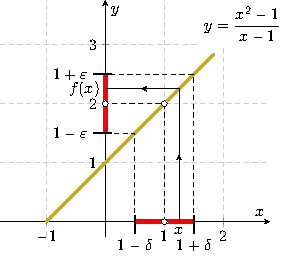
\includegraphics[width=0.45\linewidth]{mai_fig017.pdf}
   \captionof{figure}{K příkladu \ref{MAI:exam028}
   \cite[s.~118]{Brabec1989}
   \label{mai:fig017}}
  \par}
  
  Zvolíme-li libovolně malé okolí bodu \(2\), pak vždy lze najít okolí bodu \(1\) takové, že pro 
  každé \(x \neq 1\) z tohoto okolí bude ležet hodnota \(f(x)\) ve zvoleném okolí čísla \(2\). 
  Ještě jinak formulováno: K libovolně malému \(\varepsilon > 0\) existuje \(\delta > 0\) tak, 
  že pro každé \(x\), pro něž \(0 < \abs{x — 1} \ll \delta\), platí \(\abs{f(x) — 2} < 
  \varepsilon\) (viz obr. \ref{mai:fig017}). O funkci \(f\) s touto vlastností říkáme, že má v bodě 
  \(1\) limitu \(2\) a píšeme symbolicky \(lim_{x \to 1}f(x) = 2\) nebo \(f(x) \rightarrow 2\) pro 
  \(x \rightarrow 1\).
\end{example}
















    %-------------------------------------

    Definičním oborem funkce z příkladu \ref{MAI:exam028} je tedy množina \(\mathcal{D} = \realset 
    — {1}\) (pro \(a = 1\) by ve jmenovateli zlomku byla nula). Grafem funkce je tedy přímka s 
    „vynechaným“ bodem \([1, 2]\) (obr. \ref{mai:fig017}). V bodě \(a = 1\) funkční hodnota není 
    definována. Pokud bychom chtěli rozšířit definiční obor funkce na celou reálnou osu, musíme 
    předepsat, jaké hodnoty má funkce nabývat v bodě \(a = 1\). Původní vzorec, jímž je funkce 
    zadána, výpočet hodnoty \(f(1)\) neumožňuje. Dodatečné zadání funkční hodnoty, její 
    \emph{dodefinování}, můžeme provést zcela libovolně. Zvolme například \(f(1) = 2\). Jiná 
    možnost, jak funkci dodefinovat, je například \(f(1) =-1\). Které číslo je ovšem limitou funkce 
    \(f(x)\) v bodě \(a = 1\)? Je to číslo \(2\), které je v případe \(f(x) = x+1\) její funkční 
    hodnotou? Nebo číslo \(-1\)? A nebo nějaká jiná hodnota? Intuice nám napovídá, že je to číslo 
    \(2\). Když dvojku použijeme pro dodefinování funkce, přetržený graf se „zacelí“. Vidíme, že 
    vezmeme-li dostatečně malý interval proměnné \(x\) v blízkosti bodu \(a=1\) můžeme docílit 
    toho, že všechny odpovídající funkční hodnoty \(f(x)\) budou ležet tak blízko hodnotě \(2\), 
    jak si předem určíme. Skutečně, zkusme docílit toho, aby hodnoty \(f(x)\) ležely v intervalu 
    \((\num{1.99}, \num{2.01})\), tj.
    \begin{equation*}
      \num{1.99} < x + 1 < \num{2.01} \Rightarrow \num{0.99} < x < \num{1.01},\qquad x\neq1.
    \end{equation*}
    Podařilo se. A kdybychom interval \(I(\varepsilon) = (2 - \varepsilon, 2 + \varepsilon)\) 
    funkčních hodnot kolem \(2\) ještě zmenšili, podařilo by se opět najít (o něco menší) interval 
    kolem bodu \(a = 1\) tak, aby pro všechny hodnoty \(x\) v něm (samozřejmě s případnou výjimkou 
    hodnoty \(a =2\)) platilo \(f(x)\in I(\varepsilon)\). A takto bychom mohli \(\varepsilon\) 
    stále zmenšovat. Jak by takový postup dopadl s hodnotou \(-1\), která, jak intuitivně cítíme, 
    limitou funkce v bodě \(a = 1\) není, protože je graf funkce od bodu \([-1,0]\) dost vzdálen? 
    Vezměme třeba interval (\num{-0.5}, \num{0.5}) a hledejme hodnoty \(x\) obdobně jako v 
    předchozím případě. Požadujeme
    \begin{equation*}
      \num{-0.5} < x + 1 < \num{0.5} \Rightarrow \num{-1.5} < x < \num{-0.5}.
    \end{equation*}
    Tento interval vůbec neobsahuje bod \(a = 1\). Dostali jsme se mimo blízkost bodu \(a = 1\).

    %-------------------------------------
      % !TeX spellcheck = cs_CZ
\begin{mathexam}{Najdi limitu funkce \(\varphi(x) = \sqrt[3]{x}\) v bodě \(a = 0\) pomocí
  \eqref{mai:eq037}}{exam029} 
   
  Nechť \(\varphi(x) = \sqrt[3]{x}\), \(a = 0\). Pak \[f(x) = \dfrac{\sqrt[3]{x}}{x}\]. Pro \(x \neq
  0\) je \[f(x) = \frac{1}{\sqrt[3]{x^2}}\]. Jestliže \(x \to 0\), pak hodnoty \(f(x)\) neomezeně
  vzrůstají, protože jmenovatel zlomku se blíží kladnými hodnotami k nule a čitatel je stále roven
  \(1\) (viz obr. \ref{mai:fig018}). Místo rčení \emph{„funkce neomezeně roste“} pro \(x \to 0\)
  říkáme též ]\emph{„funkce se blíží k \(+\infty\)“} pro \(x \to 0\) a píšeme 
  \begin{equation*}
    \lim\limits_{x\to 0} f(x) = +\infty \text{ nebo } f(x)\to +\infty\text{ pro } x\to0.
  \end{equation*}
  Říkáme, že limita funkce \(f\) v bodě \(0\) je rovna \(+\infty\). 
    
  {\centering
  \captionsetup{type=figure}
%   \documentclass[11pt]{standalone}
\usepackage{xltxtra}
\usepackage[usenames,x11names]{xcolor}
\usepackage{tikz}
  \usetikzlibrary{intersections}
  \usetikzlibrary{decorations.markings}
\usepackage{pgfplots}
  \pgfplotsset{compat=newest}
  
\usepackage{amsmath}

\begin{document}
  \begin{tikzpicture}[thick,scale=0.7, 
      every node/.style={transform shape},
      ]
  
  \tikzset{->-/.style={decoration={
    markings,
    mark=at position #1 with {\arrow{stealth}}},postaction={decorate}}}
    
    \begin{axis}[
      xmin = -2.5, xmax = 2.5, ymin = 0, ymax = 3.5,  % osy
      domain = -1:3.5,
      restrict y to domain=0:3.4,
      axis equal image,
      grid = major,   % both
      grid style={line width=.1pt, draw=gray!20},
      major grid style={dashed, line width=.2pt, draw=gray!40},
      clip = true,
      clip mode=individual,
      xtick={-2,-1,1,2,3,4}, % make steps of length 0.2
      ytick={0,1,2,3,4,5}, 
      axis x line = middle,
      axis y line = middle,
      xlabel={\(x\)}, ylabel={\(y\)},
      enlarge y limits={rel=0.07},
      enlarge x limits={rel=0.07},
      ]
  
        \addplot[color=Gold3, samples=100, smooth, ultra thick, unbounded coords=jump,
                 no markers, domain = 0.1:2, name path global=func1] 
           gnuplot{1/((x^2.0)^(1/3.0))};
  
        \addplot[color=Gold3, samples=100, smooth, ultra thick, unbounded coords=jump,
                 no markers, domain = -2:-0.1, name path global=func2] 
           gnuplot{real(1/((x^2.0)^(1/3.0)))};
  
        \node [fill=white] at (rel axis cs: 0.75,0.5) {\(y=\dfrac{1}{\sqrt[3]{x^2}}\)};
  
        \path[name path=line] (-1,1.5) -- (1,1.5); 
            % Intersections points
            \path [name intersections={of=func1 and line,by={P1}}] (P1) node [] {};
  
        \path[name path=line] (-1,1.5) -- (1,1.5); 
            % Intersections points
            \path [name intersections={of=func2 and line,by={Q1}}] (Q1) node [] {};
        
        \draw[black,fill=black] (P1) circle (.3ex);
        \draw[black,fill=black] (Q1) circle (.3ex);
        \path (P1 |- 3,0) -- (P1) -- (P1 -| 0,3) node (X) {};
  
        \draw[thick,red, fill=white] ([shift=(0:1mm)]X) arc (0:180:1mm);
        \draw[->-=.5, dashed]  (P1 |- 3,-0.1)  
          node[below] {\(\delta\)} -- (P1) -- (P1 -| 0,3);
        \draw[->-=.5, dashed]  (Q1 |- -3,-0.1) 
          node[below] {\(\delta\)} -- (Q1) -- (Q1 -| 0,3);
  
        \draw[line width = 2pt, red, line cap=butt] (Q1 |- 3,0) -- (P1 |- 3,0);
        
        \path[name path=line] (-0.7,2.5) -- (0.7,2.5); 
            % Intersections points
            \path [name intersections={of=func1 and line,by={P1}}] (P1) node [] {};
            \draw[->-=.4, dashed, thin,gray] (P1 |- 3,-0.05) node[below] {\(x\)} -- (P1);
            \draw[->-=1, thin, gray] (P1) -- (P1 -| 0,3) node[left, fill=white] {\(f(x)\)};
        \draw[thick,red] (X) node[below left] {\(q\)} -- ++(0cm,2.5cm);
  
       \draw[black,fill=white] (0,0) node[below left] {\(O\)} circle (.4ex);
    \end{axis}
  \end{tikzpicture}
\end{document}
  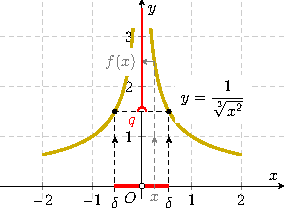
\includegraphics[width=0.8\linewidth]{mai_fig018.pdf}
  \captionof{figure}{K příkladu \ref{MAI:exam029}
  \cite[s.~118]{Brabec1989}
  \label{mai:fig018}}
  \par}
  
  Přesně to znamená toto: Zvolíme-li libovolně velké \(q > 0\), můžeme nalézt \(\delta > 0\) tak, že
  pro každé \(x \neq 0\), pro něž \(\abs{x} < \delta\), platí \(f(x) > q\). 
  
  To lze říci i takto: Zvolíme-li libovolně okolí bodu \(+\infty\), existuje okolí bodu \(0\) tak,
  že pro každé \(x \neq 0\) z tohoto okolí je \(f(x)\) ve zvoleném okolí \(+\infty\) (viz obr.
  \ref{mai:fig018}).
\end{mathexam}
















    %-------------------------------------

    Je třeba říci, že při zkoumání limit funkcí nás nezajímají jen funkce „tvaru“ 
    (\ref{mai:eq037}), i když tento případ je v diferenciálním počtu velmi častý, jak poznáme v 
    kap. \ref{mai:IchapIV}. Někdy nás zajímá i chování funkcí v okolí nevlastních bodů \(-\infty\), 
    \(+\infty\) 

    %-------------------------------------
      % !TeX spellcheck = cs_CZ
\begin{mdframed}[style=mdexam]
  \begin{example}\label{MAI:exam030}
    Je dána funkce \(f: f(x) = \frac{x + 1}{x}\). Sledujme její chování, když hodnoty argumentu
    \(x\) budou vzrůstat nade všechny meze neboli, jak říkáme, \(x\) se bude blížit k \(+\infty\)
    (což zapisujeme \(x \to + \infty\) (viz obr. \ref{mai:fig019}). Můžeme psát \(f(x) = 1 + 1/x\).
    Vzrůstají-li neomezeně hodnoty proměnné \(x\), blíží se hodnoty výrazu \(1/x\) čím dál tím více
    nule, takže funkční hodnoty \(f(x)\) jsou čím dál tím blíže číslu \(1\). V tomto případě píšeme
    \(lim_{x\to+\infty} f(x) = 1\) nebo \(f(x) \to 1\) pro \(x\to +\infty\) a říkáme, že funkce
    \(f\) má v bodě \(+\infty\) limitu rovnou \(1\). Přesně to znamená toto: Zvolíme-li libovolně
    malé \(\varepsilon > 0\), můžeme nalézt \(p > 0\) tak, že pro \(x > p\) platí \(\abs{f(x) - l} <
    \varepsilon\). (Viz obr. \ref{mai:fig019}.) Můžeme to říci i takto: Zvolíme-li libovolně okolí
    bodu \(1\), existuje okolí bodu \(+\infty\) tak, že pro každé \(x\) (konečné) z tohoto okolí je
    \(f(x)\) ve zvoleném okolí bodu \(1\).
    
    {\centering
    \captionsetup{type=figure}
  %   % !TeX spellcheck = cs_CZ

\documentclass[11pt]{standalone}
\usepackage{xltxtra}
\usepackage[usenames,x11names]{xcolor}
\usepackage{tikz}
  \usetikzlibrary{intersections}
  \usetikzlibrary{decorations.markings}
\usepackage{pgfplots}
  \pgfplotsset{compat=newest}
  
\usepackage{amsmath}

\begin{document}
  \begin{tikzpicture}[thick,scale=0.7, 
      every node/.style={transform shape},
      ]
  
  \tikzset{->-/.style={decoration={
    markings,
    mark=at position #1 with {\arrow{stealth}}},postaction={decorate}}}
    
    \begin{axis}[
      xmin = -0.5, xmax = 5.5, ymin = 0, ymax = 4.5,  % osy
      domain =0.2:5,
      restrict y to domain=0:4,
      axis equal image,
      grid = major,   % both
      grid style={line width=.1pt, draw=gray!20},
      major grid style={dashed, line width=.2pt, draw=gray!40},
      clip = true,
      clip mode=individual,
      xtick={1,2,3,4,5}, % make steps of length 0.2
      ytick={0,1,2,3,4}, 
      axis x line = middle,
      axis y line = middle,
      xlabel={$x$}, ylabel={$y$},
      enlarge y limits={rel=0.07},
      enlarge x limits={rel=0.07},
      ]
  
      \addplot[color=Gold3, samples=100, smooth, ultra thick, unbounded coords=jump,
               no markers, domain = 0.1:5, name path global=func1] 
         gnuplot{1+1/x};
  
      \node [fill=white] at (rel axis cs: 0.4,0.75) {\(y=\dfrac{x+1}{x}\)};
  
      \path[name path=line] (0,1.7) -- (3,1.7); 
          % Intersections points
          \path [name intersections={of=func1 and line,by={P1}}] (P1) node [] {};
      
      \draw[black,fill=black] (P1) circle (.3ex);      
      \path (P1 |- 3,-0.1) node [below, fill=white] (X) {p} -- (P1) -- (P1 -| 0,3);
  
      \draw[thick,red, fill=white] ([shift=(90:2.5mm)]X) 
           arc (270:360:1mm) node(Y) {} arc (360:450:1mm);
      \draw[thin] (P1 |- 3,-0.1) -- (P1) -- (P1 -| 0,3);
      \draw[line width = 2pt,red] (Y |- 3,0)  -- ++(3.5,0);
      
   
      \draw[line width = 1pt, black, dashed] (0,1) -- ++(5,0);
      \draw[line width = 3pt, red, line cap=butt] (0,0.3) -- (0,1.7);
      \draw [thick] (-.2, 0.3) node[left] {\(1-\varepsilon\)} -- (0.1, 0.3);
      \draw [thick] (-.2, 1.7) node[left] {\(1+\varepsilon\)} -- (0.1, 1.7 );
  
      \draw[black,fill=white] (0,1) circle (.4ex);

      \path[name path=line] (2.4,0) -- ++(0,2.5); 
          % Intersections points
          \path [name intersections={of=func1 and line,by={P1}}] (P1) node [] {};
          \draw[->-=.4, dashed, gray] (P1 |- 3,-0.05) node[below] {\(x\)} -- (P1);
          \draw[->-=1,  dashed, gray] (P1) -- (P1 -| 0,3) 
            node[left] {\small\(f(x)\)};
            
    \end{axis}
  \end{tikzpicture}
\end{document}
    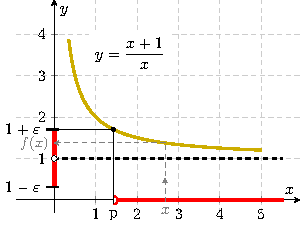
\includegraphics[width=0.45\linewidth]{mai_fig019.pdf}
    \captionof{figure}{K příkladu \ref{MAI:exam030}
    \cite[s.~119]{Brabec1989}
    \label{mai:fig019}}
    \par}
  \end{example}
\end{mdframed}
















    %-------------------------------------
    
    %-------------------------------------
      % !TeX spellcheck = cs_CZ
\begin{mdframed}[style=mdexam]
  \begin{example}\label{MAI:exam031}
    Je dána funkce \(f: f(x) = \frac{x + 1}{x}\). Sledujme její chování, když hodnoty argumentu
    \(x\) budou vzrůstat nade všechny meze neboli, jak říkáme, \(x\) se bude blížit k \(+\infty\)
    (což zapisujeme \(x \to + \infty\) (viz obr. \ref{mai:fig019}). Můžeme psát \(f(x) = 1 + 1/x\).
    Vzrůstají-li neomezeně hodnoty proměnné \(x\), blíží se hodnoty výrazu \(1/x\) čím dál tím více
    nule, takže funkční hodnoty \(f(x)\) jsou čím dál tím blíže číslu \(1\). V tomto případě píšeme
    \(lim_{x\to+\infty}f(x) = 1\) nebo \(f(x) \to 1\) pro \(x\to +\infty\) a říkáme, že funkce \(f\)
    má v bodě \(+\infty\) limitu rovnou \(1\). Přesně to znamená toto: Zvolíme-li libovolně malé
    \(\varepsilon > 0\), můžeme nalézt \(p > 0\) tak, že pro \(x > p\) platí \(\abs{f(x) - l} <
    \varepsilon\). (Viz obr. \ref{mai:fig019}.) Můžeme to říci i takto: Zvolíme-li libovolně okolí
    bodu \(1\), existuje okolí bodu \(+\infty\) tak, že pro každé \(x\) (konečné) z tohoto okolí je
    \(f(x)\) ve zvoleném okolí bodu \(1\).
    
    {\centering
    \captionsetup{type=figure}
  %   % !TeX spellcheck = cs_CZ
% xelatex -enable-write18 -shell-escape mai_fig020.tex
\documentclass[11pt]{standalone}
\usepackage{xltxtra}
\usepackage[usenames,x11names]{xcolor}
\usepackage{tikz}
  \usetikzlibrary{intersections}
  \usetikzlibrary{decorations.markings}
\usepackage{pgfplots}
  \pgfplotsset{compat=newest}
  
\usepackage{amsmath}

\begin{document}
  \begin{tikzpicture}[thick,scale=0.7, 
      every node/.style={transform shape},
      ]
  
  \tikzset{->-/.style={decoration={
    markings,
    mark=at position #1 with {\arrow{stealth}}},postaction={decorate}}}
    
    \begin{axis}[
      xmin = -2, xmax = 3.5, ymin = -2, ymax = 6,  % osy
      domain =-2:8,
      restrict y to domain=-1.5:6,
      axis equal image,
      grid = major,   % both
      grid style={line width=.1pt, draw=gray!20},
      major grid style={dashed, line width=.2pt, draw=gray!40},
      clip = true,
      clip mode=individual,
      xtick={-1,0,1,2,3,4}, % make steps of length 0.2
      ytick={-1,0,1,2,3,4,5,6,7,8}, 
      axis x line = middle,
      axis y line = middle,
      xlabel={$x$}, ylabel={$y$},
      enlarge y limits={rel=0.07},
      enlarge x limits={rel=0.07},
      ]
  
      \addplot[color=Gold3, samples=100, smooth, ultra thick, unbounded coords=jump,
               no markers, domain = -2:2, name path global=func1] 
         gnuplot{x^3};
  
      \node [fill=white] at (rel axis cs: 0.85,0.9) {\(y=x^3\)};
  
      \path[name path=line] (1.5,0) -- (1.5,6); 
          % Intersections points
          \path [name intersections={of=func1 and line,by={P1}}] (P1) node [] {};
          \draw[->-=.4, dashed, gray] (P1 |- 3,-0.05) node[below, fill=white] {\(x\)} -- (P1);
          \draw[->-=1,  dashed, gray] (P1) -- (P1 -| 0,3) 
            node[left=0.5cm, fill=white] {\small\(f(x)\)};
          \draw[dashed, gray] (P1 -| 0,3) + (-0.6cm,0cm) -- (P1 -| 0,3);
      \path[name path=line1] (0,1) -- (2,1); 
          % Intersections points
          \path [name intersections={of=func1 and line1, by={P1}}] (P1) node [] {};    
          \path (P1 |- 3,-0.1) node [below, fill=white] (X) {p} -- (P1) -- (P1 -| 0,3) 
              node[left, fill=white] (Y) {\(q\)};
  
      \draw[thick,red, fill=white] ([shift=(90:2mm)]X) 
           arc (270:360:1mm) node(x1) {} arc (360:450:1mm);
      \draw[dashed] (P1 |- 3,-0.1) -- (P1) -- (P1 -| 0,3);
      \draw[line width = 1pt,red] (x1 |- 3,0)  -- (3,0);
      
      \draw[thick,red] (0,1) -- (0,6);
      \draw[thick,red, fill=white] ([shift=(0:3.3mm)]Y) arc (0:180:1mm);;
    \end{axis}
  \end{tikzpicture}
\end{document}
    \includegraphics[width=0.35\linewidth]{mai_fig020.pdf}
    \captionof{figure}{K příkladu \ref{MAI:exam031}
    \cite[s.~119]{Brabec1989}
    \label{mai:fig020}}
    \par}
  \end{example}
\end{mdframed}
    %-------------------------------------
    
    V uvedených případech bychom mohli zkoumat i limity funkcí pro \(x \to - \infty\).  Všimněme si 
    ještě, že ve všech případech nebylo nutné, aby funkce \(f\) byla definována v bodě, ke kterému 
    se blíží hodnoty argumentu, ale bylo zapotřebí, aby funkce \(f\) byla definována v bodech 
    libovolně blízkých tomuto bodu. Tomuto požadavku bude vyhověno, jestliže daný bod, v němž 
    zkoumáme limitu, bude \emph{hromadným bodem definičního oboru}. Není ovšem nutné, aby funkce 
    byla definována v celém nějakém \emph{prstencovém okolí uvažovaného bodu}.
    
    Nechť \(a\) je bod, blízko kterého se pohybuje hodnota proměnné \(x\). Pro definici limity je 
    důležitý pojem \textbf{okolí bodu} \(a\) (obr. 2.16). Zvolme kladná čísla \(\delta_1\) a 
    \(\delta_2\). Nazýváme
    
    
      
  %================ Podkapitola: Spojitost funkce ==================================================
  \section{Spojitost funkce}
  
%} % tikzset
%~~~~~~~~~~~~~~~~~~~~~~~~~~~~~~~~~~~~~~~~~~~~~~~~~~~~~~~~~~~~~~~~~~~~~~~~~~~~~~~~~~~~~~~~~~~~~~~~~~
\printbibliography[title={Seznam literatury}, heading=subbibliography]
\addcontentsline{toc}{section}{Seznam literatury}          	
%---------------------Numerické metody ------------------------------------------------------------
  % !TeX spellcheck = cs_CZ
%{\tikzset{external/prefix={tikz/MAI/}}
% \tikzset{external/figure name/.add={ch10_}{}}
%---------------------------------------------------------------------------------------------------
% file mai1ch03.tex
%---------------------------------------------------------------------------------------------------
\chapter{Kombinatorika, pravděpdobnost, statistika}\label{mai:IchapIII}
\minitoc
  \section{Kombinatorika}\label{mai:IchapIIIsecI}
    \textbf{Kombinatorika} se od všech matematických disciplín, v několika směrech liší. Zatímco v 
    geometrii má každá přímka nekonečnou délku a každý trojúhelník nekonečně mnoho bodů, zatímco v 
    algebře některé rovnice i nerovnice mají nekonečně mnoho řešení a zatímco matematická analýza 
    zkoumá limity posloupností a funkcí, roste-li příslušná proměnná do nekonečna, v kombinatorice 
    se s nekonečnem nesetkáme. Kombinatorika je součástí \textbf{finitní matematiky}, která studuje 
    konečné soubory (množiny a uspořádané \(k\)-tice, \(k\in \mathcal{N}\)). 
    
    Další odlišností je to, že často nemáme možnost ověřit si správnost výsledku, ke kterému jsme 
    při řešení kombinatorické úlohy dospěli, a jsme odkázáni jen na svůj vlastní úsudek. Proto v 
    kombinatorice v míře větší než jinde platí, že „cvičení dělá mistra“. 
    
    V této kapitole je probrána část kombinatoriky, která se zabývá vytvářením skupin z daných 
    prvků a určováním jejich počtu. Jde o klasickou problematiku, která byla řešena již v 17. a 18. 
    století a která je spojena se jmény \emph{B. Pascala}, \emph{P. Fermata}, \emph{J Bernoulliho}, 
    \emph{G. W. Leibnize}  a \emph{L. Eulera}. Dnes představuje kombinatorika rozsáhlou 
    matematickou disciplínu, některé její problémy byly již vyřešeny (problém čtyř barev) mnohé 
    další na své vyřešení čekají. 
    
    A závěrem ještě důležitá poznámka terminologická: přirozeným čísly se v této kapitole rozumějí 
    čísla celá kladná tj. čísla 1, 2, 3, 4, \(\ldots\), nula se tedy mezi přirozená čísla 
    nezahrunuje. \cite[s.~7]{calda2008matematika} 
    
    \subsection{Základní kombinatorická pravidla}
    
    
    \cite[s.~7]{polak1991matematika}
    
  \section{Pravděpodobnost}\label{mai:IchapIIIsecII}
    Slovo pravděpodobnost používáme velmi často. Jaký však je jeho přesný význam? Jsme přesvědčeni, 
    že pravděpodobnost výhry ve sportce je velmi malá. Ani pravděpodobnost, že se vyplní předpověď 
    počasí, nepovažujeme mnohdy za výraznou. Přesto je mezi oběma příklady obrovský kvantitativní 
    rozdíl. Zkusme význam pojmu pravděpodobnost ukázat pomocí konkrétních číselných příkladů.
  
    \begin{itemize}
      \item \textbf{Příklad se střelcem}: Sportovní střelec střílí na terč série \num{100} ran. 
            Předpokládejme, že podmínky při střelbě jsou stále stejné. Stejná je zbraň, terč, 
            vzdálenost, povětrnostní podmínky i momentální zdravotní stav střelce. Při hodnocení 
            střelcova „mistrovství“ někdo řekne, že střelec zasáhne terč s pravděpodobností 
            \num{92}\%. Jak tomu rozumět? Znamená to, že v souboru sérií výstřelů jsou velmi časté 
            ty, v nichž zasáhl střelec terč \num{92}-krát. Samozřejmě, není řídké, že se objeví i 
            série s \num{93} nebo \num{94} zásahy, ale také s \num{91} nebo \num{90}. Vyloučen není 
            ani případ s úspěšností \num{96} či \num{88}, a dokonce i stovku bychom mohli 
            zaznamenat. Situace výrazně odlišné od \num{92} zásahů však budou řídké, a to tím více, 
            čím více se úspěšnost série liší od \num{92} oběma směry.
      \item \textbf{Příklad se zmetky}: Koupíte si výrobek u firmy, o které je známo, že vyrábí 
            zmetky s pravděpodobností 0,16\%? Situaci lze posuzovat obdobně jako úspěšnost střelce. 
            Budeme-li například zkoumat série obsahující 1000 výrobků, bude každá z nich obsahovat 
            „v průměru“ 16\% zmetků. Z příkladu se střelcem již zhruba víme, jak posuzovat slovo v 
            průměru.
    \end{itemize}
    
    V této kapitole se budeme pravděpodobnostmi zabývat podrobněji. Zjistíme, že i když se týkají 
    náhodných jevů, platí i pro ně jisté zákonitosti. V úvodních příkladech jsme si vyložili, jak 
    intuitivně chápat pojem pravděpodobnost. Jednalo se v nich o posouzení průměrné úspěšnosti ve 
    velkém souboru operací či úkonů prováděných za stejných podmínek, šlo tedy o jakousi 
    „průměrnou“ pravděpodobnost. Nyní definujeme pravděpodobnost matematicky.
    
    \subsection{Co se pravdě podobá - definice pravděpodobnosti}
      Pro definici pravděpodobnosti použijeme pojmu \emph{náhodný pokus}, jehož význam si ukážeme 
      na příkladu. Dobrým příkladem náhodných pokusů je třeba házení mincí, hraní kostkou, výběr 
      karet z balíčku, vidíme-li pouze jejich rub, apod. Budeme třeba házet kostkou. Abychom si 
      situaci zbytečně nekomplikovali, budeme předpokládat, že všechny výsledky hodu kostkou 
      (náhodné pokusy) jsou stejně časté, žádný z nich není nijak preferován\footnote{Kostka by 
      tedy měla být homogenní, plocha, na kterou po hodu dopadne, vodorovná, kvalita povrchu všech 
      stěn kostky stejná (žádná stěna by třeba neměla být natřena lepidlem), apod.}. Počet možných 
      výsledků jednotlivého hodu je \(N = 6\) (kostka má \num{6} stěn, na každé je vyznačen odlišný 
      počet ok, tedy \num{1} až \num{6}). Jednotlivé situace, které mohou nastat, nazýváme 
      náhodnými jevy. Náhodným jevem \(A\) tak může být situace \emph{„padne číslo \num{2}“}, jiným 
      náhodným jevem \(B\) situace \emph{„padne číslo dělitelné třemi“}, apod. Počet situací, kdy 
      výsledek hodu lze hodnotit tak, že určitý jev nastal, označíme \(M\). Například pro jev \(A\) 
      \emph{„padne číslo \num{2}“} je \(M(A)= 1\), pro jev \(B\) \emph{„padne číslo dělitelné 
      třemi“} je \(M(B) = 2\) (počet ok \num{3} nebo \num{6}). Můžeme také definovat jev \(O\) 
      \emph{„nepadne žádné číslo“} (\(M(0) = 0\)) nebo jev \(J\) \emph{„padne jakékoli číslo“} 
      (\(M(J) = 6\)).
      
      \begin{definition}
        Pravděpodobností jevu rozumíme podíl
        \begin{equation}\label{mai:eq011}
          p = \frac{M}{N} = \frac{\text{počet případů příznivých}}{\text{počet případů možných}}.
        \end{equation}  
        Počtem případů možných jsme zkráceně nazvali počet všech možných výsledků náhodného 
        pokusu, počtem případů příznivých pak počet všech takových výsledků pokusu, při nichž daný 
        jev nastal.
      \end{definition}
      Je zřejmé, že hodnota pravděpodobnosti jakéhokoli jevu je nezáporná a může nabývat hodnoty 
      nejvýše \num{1}, tj. \(0 <p< 1\). Jev s \emph{nulovou pravděpodobností} se nazývá 
      \textbf{nemožný}, jev s \emph{jednotkovou pravděpodobností} je \textbf{jistý}. V našem 
      příkladu s kostkou tak dostáváme
      \begin{equation*}
        p(A) = \frac{1}{6}, \qquad p(B) = \frac{2}{6} = \frac{1}{3}, \qquad
        p(O) = 0, \qquad p(J) = 1.
      \end{equation*}  

      %--Barevné ponožky----------------------------------------------
      % !TeX spellcheck = cs_CZ
\begin{example}
 \label{mai:exam006}
  \textbf{Barevné ponožky}:\newline\small
  V zásuvce jsou ponožky tří barev. Červené (\textbf{Č}), zelené (\textbf{Z}) a modré (\textbf{M}). 
  Je jich tam od každé barvy hodně. Student jde na schůzku a chce si vzít čisté ponožky. Náhle 
  zhasne světlo. Student vytáhne potmě dvě ponožky. Jaká je pravděpodobnost, že ponožky budou mít 
  stejnou barvu? Vyjmenujme případy, které mohou při vytažení dvou ponožek nastat: (\textbf{Č+Č}), 
  (\textbf{Č+Z}), (\textbf{Z+Č}), (\textbf{Č+M}), (\textbf{M+Č}), (\textbf{Z+Z}), (\textbf{Z+M}), 
  (\textbf{M+Z}), (\textbf{M+M}). Je tedy \(n = 9\). Příznivé situace jsou tří, (\textbf{Č+Č}), 
  (\textbf{Z+Z}), (\textbf{M+M}). Pravděpodobnost je tedy 1/3. (Převzato z 
  \cite[s.~200]{Musilova2009MA1}) 
\normalsize
\end{example}
      %---------------------------------------------------------------
    \subsection{Cifry, kostky, karty - kombinatorické opakování}
      Příklad s ponožkami byl velmi jednoduchý. Podařilo se nám vyjmenovat všechny případy možné i 
      všechny případy příznivé, neboť obojího bylo docela málo. Daleko běžnější jsou však situace, 
      kdy výčet případů není schůdný. A tehdy potřebujeme \textbf{kombinatoriku}.
      
      Nechť \(\mathcal{M}\) je \(n\)-prvková množina, z níž budeme provádět výběry \(k\) prvků 
      podle určitých pravidel. Prvky množiny \(\mathcal{M}\) nemusíme nijak konkretizovat. Abychom 
      si však o výběrech a pravidlech pro jejich tvorbu dokázali udělat nějakou názornou představu, 
      je taková konkretizace vhodná. Prvky množiny \(\mathcal{M}\): mohou být třeba žáci ve třídě, 
      barvy, hrací karty, apod. Výběry mohou představovat třeba družstva pro odbíjenou, signály 
      tvořené barevnými praporky, možnosti rozdání karet při mariáši, apod. Jednotlivé typy výběrů 
      získaly své názvy právě na základě pravidel stanovených pro jejich vytváření. Rozhodující 
      jsou dvě základní kritéria:
      \begin{itemize}\addtolength{\itemsep}{-0.5\baselineskip}
        \item Je pro tvorbu výběru podstatné pořadí prvků ve výběru či nikoliv?
        \item Mohou se prvky ve výběru opakovat či nikoliv?
      \end{itemize}
      
      Typy výběrů shrnuje následující diagram:
      \begin{figure}[ht!] %\ref{mai:fig021}
        \centering
        \includegraphics[width=0.7\linewidth]{mai_fig021.pdf}
        \caption{Typy výběrů. \cite[s.~201]{Musilova2009MA1}}
        \label{mai:fig021}
      \end{figure}

      Představuje-li daný výběr například volejbalové družstvo osmi děvčat (šest hráček a dvě 
      náhradnice), které bude reprezentovat v soutěži třídu osmou bé, do níž chodí \num{25} děvčat 
      a \num{18} chlapců, jedná se o výběr \(k - 8\) prvků z počtu \(n = 25\) prvků. Chlapce nelze 
      postavit do družstva volejbalistek. Každý výběr možného družstva bude představovat 
      \emph{kombinaci bez opakování}, neboť pořadí hráček nehraje roli a třeba Aničku Novákovou 
      máme ve třídě jen jednu. Budeme-li však chtít vytvářet z deseti cifer \(0, 1, \ldots, 9\) 
      trojciferná čísla, pak tyto výběry tří prvků z deseti (\(k = 3\), \(n = 10\)) jsou 
      \emph{variacemi s opakováním}. Čísla \num{125}, \num{512}, \num{251}, \num{215}, \num{521} a 
      \num{152} jsou totiž různá, a například \num{222} je také trojciferné číslo. Kombinace s 
      opakováním bychom mohli vytvářet třeba i při výběru různobarevných ponožek ze zásuvky a 
      konečně \emph{variacemi bez opakování} by mohly být dejme tomu trojbarevné signály (\(k = 
      3\)) tvořené trojicemi barevných hadříků vybíraných z \(n\) barev (pro \(n = 3\) třeba zrovna 
      z těch ponožek). Nyní bychom však rádi věděli, jak pro zadané hodnoty \(n\) a \(k\) určit 
      počet všech možných výběrů předepsaného typu. Ukážeme si to na příkladech.

      %--Šance milion-------------------------------------------------
      % !TeX spellcheck = cs_CZ
\begin{mdframed}[style=mdexam]
  \begin{example}\label{mai:exam007}
    \textbf{Šance milion}:\newline
    „Znáte nějakou jinou hru, kde můžete denně vyhrát milion?“ Tento nebo jiný, obdobně nepříliš
    vtipný reklamní slogan propaguje v televizi hru, jejímž cílem je uhodnout šestici tažených cifer
    ve správném pořadí. (Hru raději nehrajte, pravděpodobnost výhry je mizivá.) Tah se provádí
    následovně: V každém ze šesti bubnů, očíslovaných pořadovými čísly \num{1} až \num{6}, je
    připraveno deset míčků opatřených ciframi \(0, 1, \ldots, 9\). Z prvního bubnu se náhodně
    vylosuje jedna cifra (deset možností). Poté se náhodně vylosuje jedna cifra z druhého bubnu
    (opět deset možností). Možností vzniku uspořádané dvojice cifer (jedna cifra z prvního a druhá z
    druhého bubnu) je již sto (každou možnost výsledku u prvního bubnu lze kombinovat s každou
    možností výsledku z druhého bubnu). Losování pokračuje u třetího, čtvrtého, pátého a šestého
    bubnu. Celkový počet možností je \num{1e6}, tedy \textbf{milion}. (Šance získat výhru, tedy
    vyhrát milion, je ovšem pouze jedna milióntina, neboť z milionu možností je pouze jedna skutečně
    tažena.) 
  \end{example}
\end{mdframed}
      %---------------------------------------------------------------
      
      Zobecněním předchozího příkladu získáváme vzorec pro počet \textbf{variací s opakováním} 
      \emph{k}-té třídy z \(n\) prvků. Při tahu totiž záleží na pořadí bubnů a každý buben obsahuje 
      všechny cifry. Výsledky tahů z jednotlivých bubnů se tedy mohou opakovat. Pokud by bubnů bylo 
      \(k\) a v každém \(n\) různých cifer, dostali bychom pro \textbf{variace s opakováním 
      \(k\)-té třídy z \(n\) prvků} celkový počet
      \begin{equation}\label{mai:eq007}
        \boxed{V_k' = n^k}\, .
      \end{equation}

      %--Modifikovaná šance milion------------------------------------
      % !TeX spellcheck = cs_CZ
\begin{example}\label{mai:exam008}
  \textbf{Modifikovaná šance milion}:\newline
  Představme si hru z předchozího příkladu upravenou takto: K dispozici bude jen jeden buben s 
  ciframi \(0, 1, \ldots, 9\), každá cifra je v bubnu obsažena pouze jednou. Opět máme losovat 
  uspořádanou \textbf{šestici cifer}. Nyní se však jedná o \textbf{variace šesté třídy z deseti 
  prvků bez opakování}. S jediným bubnem musíme totiž provést šest losování, přičemž při každém 
  losování ubude z bubnu jedna cifra. Při prvním tahu je deset možností, při druhém již jen devět, 
  atd., při šestém již pouze pět možností. Celkem je tedy \(10 \cdot 9 \cdots 5 = \num{151200}\) 
  možností.
\end{example}
      %---------------------------------------------------------------
      
      Uvážíme-li, že v předchozím příkladu je \(n = 10\) a \(k = 6\), dostáváme pro \textbf{počet 
      variací bez opakování \(k\)-té třídy z \(n\) prvků} obecný vztah
      \begin{align}
        V_k(n) &= n(n-1)(n-2)\cdots(n-k+1)  \nonumber \\
        \shortintertext{neboli}
        V_k(n) &= \frac{n!}{(n-k)!}\, .    \label{mai:eq008}
      \end{align}
      Poznamenejme, že \(n!\) značí \textbf{faktoriál}, \(n! = n(n - 1)\cdots 3 \cdot 2 \cdot 1\). 
      Pro nulu definujeme \(0! = 1\). Je zřejmé, že při vytváření variací bez opakování musí být 
      \(k\leqq n\). Variace bez opakování \(n\)-té třídy z \(n\) prvků se nazývají 
      \textbf{permutace}. Každá z nich představuje určité uspořádání těchto \(n\) prvků. Platí
      \begin{equation}\label{mai:eq009}
        \boxed{P(n) = V_n(n) = n!}\, .
      \end{equation}
      
      Nyní odvodíme vzorec pro počet \textbf{kombinací \(k\)-té třídy z \(n\) prvků bez opakování}. 
      Již jsme si řekli, že \emph{kombinací} rozumíme takový výběr z celkového počtu \(n\) prvků, 
      který obsahuje určitých \(k\) prvků nezávisle na jejich pořadí. Představme si, že máme k 
      dispozici všechny variace bez opakování \(k\)-té třídy ze zmíněných \(n\) prvků. Vezměme 
      kteroukoli z nich. Soubor všech variací \(k\)-té třídy z \(n\) prvků však obsahuje i další 
      variace, lišící se od té naší jen pořadím prvků. Celkem je takových variací (i s tou první) 
      \(k!\) a z hlediska kombinací představují totéž. Soubor variací se tak rozpadá na podsoubory, 
      z nichž každý obsahuje \(k!\) variací lišících se navzájem pouze pořadím prvků. Každý z 
      těchto podsouborů představuje však jedinou kombinaci. Počet kombinací \(k\)-té třídy z \(n\) 
      prvků bez opakování je tedy
      \begin{equation}\label{mai:eq010}
        \boxed{C(k) = \frac{V_k(n)}{P(k)} = \frac{n!}{(n-k)!\,k!} = 
               \begin{pmatrix}
                n \\
                k
               \end{pmatrix}}\, .
      \end{equation}
      
      Pro odvození vzorce pro \textbf{kombinace s opakováním} použijeme opět příkladu.
      %--Kuličky v přihrádkách----------------------------------------
      % !TeX spellcheck = cs_CZ
\begin{mathexam}{Kuličky v přihrádkách}{exam009}
  Máme kuličky \(n\) různých barev, v každé barvě máme tolik kuliček, kolik bude potřeba. Naším
  úkolem je vytvářet výběry \(k\) kuliček. Na \textbf{pořadí barev nezáleží}, kuliček jedné barvy
  může být ve výběru libovolný počet \(0\leqq s \leqq k\). Výběry budeme vytvářet tak, že budeme
  kuličky dávat do \(n\) přihrádek, z nichž každá bude vyhrazena pro určitou barvu. Pokud tedy v
  daném výběru zrovna nebude třeba modrá kulička, bude přihrádka vyhrazená pro modrou barvu prázdná.
  Budou-li v daném výběru právě tři červené kuličky, budou umístěny v přihrádce vyhrazené pro
  červenou barvu. Vidíme, že pokud konkrétním přihrádkám přisoudíme konkrétní barvy, samotné kuličky
  by již barevné být nemusely, stačily by třeba kuličky skleněné, bezbarvé. Zůstane-li například
  přihrádka pro modrou barvu prázdná, víme, že daný výběr neobsahuje modrou barvu. Budou-li v
  přihrádce pro červenou barvu tři (bezbarvé) kuličky, víme, že daný výběr obsahuje červenou barvu
  třikrát. Příklad takové situace ukazuje následující schéma:
  
  {\centering
    \luafigure[0.9]{mai_fig033.pdf}
    \par}

  Náš úkol můžeme přeformulovat takto: Je třeba rozmístit \(k\) kuliček do \(n\) přihrádek. V každé
  přihrádce může být obecně \(s\) kuliček, kde \(0\leqq s \leqq k\), přitom celkový počet kuliček
  musí být samozřejmě stále \(k\). Můžeme si představit, že \(k\) kuliček máme položených v řadě na
  polici mezi dvěma pevnými stěnami (krajní svislé čáry v předchozím schématu) a různé způsoby
  rozmístění kuliček do přihrádek provádíme přemísťováním pohyblivých přepážek. Kdybychom například
  v předchozím schématu přesunuli druhou svislou čáru, počítáno zleva, až za první kuličku v
  přihrádce na červenou barvu, dostaneme uspořádání, při němž je v přihrádce na modrou barvu jedna
  kulička a v přihrádce na červenou barvu dvě kuličky. Tedy takto:

  {\centering
    \luafigure[0.9]{mai_fig034.pdf}
  \par}

  Mezi dvěma krajními pevnými stěnami máme tedy k dispozici \(k\) pozic pro kuličky a \((n - 1)\)
  pozic pro pohyblivé přepážky. Celkem tedy \((n + k - 1)\) pozic, na které můžeme libovolně
  rozmísťovat \(k\) kuliček a \((n - 1)\) přepážek. Do těchto \((n + k - 1)\) pozic můžeme umístit
  \(k\) kuliček \(C_k'(n)\) způsoby, kde
  \begin{equation}\label{MAI:eq011}
    \boxed{C_k'(n) =  \binom{n + k - 1}{k} = \binom{n + k - 1}{n -1}}\, .
  \end{equation}
  Na zbylé pozice již musíme umístit přepážky. Nebo naopak, nejprve umístíme \((n - 1)\) přepážek a
  potom kuličky. Výsledek je stejný, jak je vidět z předchozího vzorce. Protože jsme vytváření
  kombinací s opakováním \(k\)-té třídy z \(n\) prvků převedli na úlohu o rozmísťování kuliček do
  přihrádek, udává získaný vzorec právě počet takových kombinací. Aby měl vzorec smysl, musí platit
  \(n + k - 1 \geqq k\), tedy \(n \geqq 1\).

  Komu nevyhovuje představa kuliček v přihrádkách a má raději čísla, může uvažovat následovně: Tak
  jako je každé číslo v desítkové soustavě zapsáno pomocí cifer \(0, 1, 2, \ldots , 8, 9\), je k
  jeho zápisu ve dvojkové soustavě potřeba pouze dvou cifer, nuly a jedničky. Představme si nyní
  přepážku jako jedničku a kuličku jako nulu. Náš úkol zjistit počet všech možných způsobů rozdělení
  \(k\) kuliček do \(n\) přihrádek, ohraničených \((n+1)\) přepážkami, můžeme převést na
  ekvivalentní problém: Kolik dokážeme najít čísel, která jsou ve dvojkové soustavě zapsána právě
  \(k\) nulami a \((n + 1)\) jedničkami, požadujeme-li, aby první i poslední cifrou byla jednička?
  Odpověď je jednoduchá. Máme k dispozici \((n+k+1)\) pozic pro cifry. První a poslední pozice jsou
  pevně obsazeny jedničkami, volných pozic je tedy pouze \((n + k - 1)\). Počet všech různých
  způsobů, kterými na \(k\) z těchto pozic můžeme umístit nuly, je roven počtu kombinací \(k\)-té
  třídy z \((n + k - 1)\) prvků. Na zbylé pozice již musíme umístit jedničky. Komplementárně,
  budeme-li hledat počet všech možných způsobů, jak na \((n-1)\) pozic umístit jedničky, dostaneme
  shodný výsledek, v souhlasu se vzorcem (\ref{mai:eq010}).
\end{mathexam}
      %---------------------------------------------------------------
      
      %--Obsazování kvantových stavů----------------------------------
      % !TeX spellcheck = cs_CZ
\begin{example}\label{mai:exam010}
  \textbf{Obsazování kvantových stavů}:\newline\small
  Úloha o kuličkách a přihrádkách má přímou aplikaci v \textbf{kvantové fyzice}. Představme si, že 
  fyzikální soustava je tvořena \(k\) částicemi. Každá částice se nachází v určitém stavu, v němž 
  jí můžeme přisoudit fyzikální charakteristiky, které jsou s tímto stavem spojeny (třeba energii, 
  moment hybnosti, apod.). Jednotlivé stavy jsou pak rozlišitelné právě pomocí těchto 
  charakteristik. Dejme tomu, že přípustných stavů je \(n \geqq 1\). Problémem kvantové fyziky je 
  to, že kvantové částice jsou nerozlišitelné. Nepoznáme jednu od druhé. Je to stejné, jako bychom 
  měli \(k\) naprosto stejně vypadajících kuliček, které nemáme nijak očíslovány. Záměna dvou 
  částic (nerozlišitelných kuliček) se nepozná, nevede tedy ke změně stavu fyzikální soustavy. Pro 
  hodnoty fyzikálních charakteristik soustavy jako celku je tedy důležité jen to, kolik částic je v 
  každém z přípustných stavů. Musíme se tedy zajímat o to, kolika způsoby lze našich \(k\) 
  \textbf{nerozlišitelných částic} (kuliček) umístit do \(n\) \textbf{stavů} (přihrádek). Kvantové 
  částice jsou však dvojího druhu, \textbf{fermiony} (například elektrony, neutrony, protony, jádra 
  s lichým počtem nukleonů) a \textbf{bosony} (například fotony, mezony, jádra se sudým počtem 
  nukleonů). Rozdíl mezi nimi je ten, že bosony se „dobře snášejí“, a proto jich může být v jednom 
  stavu i více. 
  \begin{itemize}\addtolength{\itemsep}{-0.5\baselineskip}
    \item Počet možností, jak rozmístit \(k\) \textbf{bosonů} po \(n\) stavech je tedy
          \begin{equation*}
            N_{\text{boson}} = 
              \begin{pmatrix}
                n + k - 1 \\
                    k
               \end{pmatrix}
          \end{equation*}
    \item S \textbf{fermiony} je tomu jinak. \textbf{Pauliho vylučovací princip} jim zakazuje, 
          aby v daném stavu byl více než jeden fermion. Stav může být buď prázdný, nebo obsazen 
          jedním fermionem. V takovém případě musí být \(n \geqq k\) a v každé přihrádce může být 
          nejvýše jedna kulička. Situace tak odpovídá \textbf{kombinacím bez opakování \(k\)-té 
          třídy z \(n\) prvků}, tj.
          \begin{equation*}
            N_{\text{fermion}} = 
              \begin{pmatrix}
                n  \\
                k
              \end{pmatrix}
          \end{equation*}
  \end{itemize}
\normalsize
\end{example}
      %---------------------------------------------------------------
      
      Získané kombinatorické vzorce nyní použijeme při řešení základních úloh o pravděpodobnostech. 
      V každé úloze bude důležité
      \begin{itemize}
        \item definovat jev \(A\), jehož pravděpodobnost počítáme,
        \item určit počet \(N\) případů možných, tj. počet všech možných výsledků pokusu, při 
              kterém sledujeme, zda jev \(A\) nastal či nenastal,
        \item určit počet \(M\) případů příznivých, tj. počet těch výsledků daného pokusu, při 
              kterých jev \(A\) nastal.
      \end{itemize}

      %--Výhra ve sportce---	----------------------------------------
      % !TeX spellcheck = cs_CZ
\wikitextrule
\begin{example}\label{mai:exam052}
  \textbf{Výhra ve sportce}\newline\small
  Jaká je pravděpodobnost hlavní výhry ve sportce? Všichni víme, že malá, ale máme představu, jak 
  malé toto číslo je? Při sportce se losuje \(k = 6\) čísel a jedno dodatkové z celkového počtu \(n 
  = 49\) čísel. (Dříve byla čísla spojena s názvy sportů, odtud název „sportka“ .) Na pořadí čísel 
  ve výběru nezáleží, vytažené číslo se do hry nevrací. Jde tedy o \textbf{kombinace bez 
  opakování}. Hlavní výhra požaduje uhodnout všech \num{6} tažených čísel. Jev \(A\) je tedy 
  definován takto:
  
  \begin{itemize}
    \item Jev \(A\): Bude taženo právě oněch \num{6} čísel, která jsem vsadil.
          Počet možností, které při tahu sportky mohou nastat (počet případů možných), je \(N = 
          \begin{pmatrix} n \\ k\end{pmatrix} =  \begin{pmatrix} 49 \\ 6 \end{pmatrix} \). Hlavní 
          výhru představuje jediná kombinace, počet příznivých případů je proto \(M = 1\). 
          Pravděpodobnost hlavní výhry ve sportce, tj. pravděpodobnost jevu \(A\), je
          \begin{equation*}
            p(A) = \dfrac{M}{N} = \dfrac{1}{\begin{pmatrix} 49 \\ 6 \end{pmatrix}} 
                 = \dfrac{43!6!}{49!} = \dfrac{720}{49\cdot48\cdot47\cdot46\cdot45\cdot44} \simeq 
                 \num{7e-8}
                 = \SI{7e-6}{\percent}
          \end{equation*}
          Pravděpodobnost hlavní výhry je velmi malá, sedm milióntin procenta. 
    \item A o kolik lepší to bude s pravděpodobností některé z vedlejších výher? Tak třeba pátá 
          cena znamená, že je nutné ze šesti tažených čísel uhodnout libovolné tři. Jev \(A\) je 
          tedy: Ze šesti čísel, která jsme vsadili, budou v tažené kombinaci obsažena právě tři 
          libovolná z nich. Počet \(N\) zůstává stejný jako v předchozí části úlohy. Je třeba jen 
          určit \(M\). Každý příznivý případ vzniká tak, že trojice správných čísel (výběry tří ze 
          šesti) je doplněna trojicí chybných čísel (výběry tří ze čtyřiceti tří). Tedy \(M = 
          \begin{pmatrix}6 \\ 3\end{pmatrix}\begin{pmatrix} 49 - 6 \\ 3\end{pmatrix} =  
          \begin{pmatrix} 6 \\ 3\end{pmatrix}\begin{pmatrix} 43 \\ 3 \end{pmatrix}\),
          \begin{align*}
            p(A) &= \dfrac{M}{N} 
                  = \dfrac{\begin{pmatrix} 6 \\ 3\end{pmatrix}
                           \begin{pmatrix} 43 \\ 3 \end{pmatrix}}
                          {\begin{pmatrix} 49 \\ 6\end{pmatrix} }                
                  =\left(\dfrac{6!}{3!\cdot3!}\right)\left(\dfrac{43!}{40!\cdot3!}\right)
                   \left(\dfrac{43!6!}{49!}\right)                                            \\
                 &=\dfrac{120\cdot43\cdot42\cdot41\cdot720}
                         {49\cdot48\cdot47\cdot46\cdot45\cdot44\cdot36} 
                  \simeq\num{0.018}.
          \end{align*}
          Tato pravděpodobnost již zanedbatelná není, na rozdíl od finanční částky, jíž bývá 
          ohodnocena pátá cena. Sázení sportky může domácímu rozpočtu spíše ublížit.
    \item Třetí, resp. čtvrtá cena jsou, podobně jako první a pátá, definovány velmi jednoduše. Je 
          třeba uhodnout pět, resp. čtyři ze šesti tažených čísel. V případě druhé ceny hraje roli
          dodatkové číslo. Druhou cenu získává ten, kdo uhodl pět ze šesti čísel vylosovaných v 
          prvním tahu a ještě navíc číslo dodatkové, které se losuje ze zbylých \num{43} čísel, jež 
          zůstala po prvním tahu v osudí. Jev \(A\) je tedy definován takto:
          
          Ze šesti čísel, která jsem vsadil, bude při prvním tahu vylosováno libovolných pět a v 
          druhém tahu bude vylosováno právě to dodatkové číslo, které jsem vsadil. Počet případů 
          příznivých je pouze \(M = \begin{pmatrix}6 \\ 5\end{pmatrix}\), neboť šestým číslem 
          nemůže být libovolné ze \num{43} čísel, která nebyla v prvním tahu vylosována, ale 
          musí to být právě číslo dodatkové. Pravděpodobnost jevu \(A\) je
          \begin{equation*}
            p(A)  = \dfrac{M}{N} 
                  = \dfrac{\begin{pmatrix} 6  \\ 5\end{pmatrix}}
                          {\begin{pmatrix} 49 \\ 6\end{pmatrix}}
                  \simeq\num{4.2e-17}.
          \end{equation*}
          
          Pokud bychom jako jev \(A\) označili výhru jakékoliv ceny, dostaneme
          \begin{align*}
            M &= \sum_{6}^{k=3}\begin{pmatrix} 6  \\   k  \end{pmatrix}
                               \begin{pmatrix} 43 \\ 6 - k\end{pmatrix}  +
                               \begin{pmatrix} 6  \\   5  \end{pmatrix}                      \\
              &= \begin{pmatrix} 6 \\ 3\end{pmatrix}\begin{pmatrix} 43 \\ 3\end{pmatrix} +
                 \begin{pmatrix} 6 \\ 4\end{pmatrix}\begin{pmatrix} 43 \\ 2\end{pmatrix} +
                 \begin{pmatrix} 6 \\ 5\end{pmatrix}\begin{pmatrix} 43 \\ 1\end{pmatrix} +
                 \begin{pmatrix} 6 \\ 6\end{pmatrix}\begin{pmatrix} 43 \\ 0\end{pmatrix} +
                 \begin{pmatrix} 6 \\ 5\end{pmatrix},                                        \\
           p(A) &= \dfrac{\begin{pmatrix}  6 \\ 3\end{pmatrix}
                          \begin{pmatrix} 43 \\ 3\end{pmatrix}  +
                          \begin{pmatrix}  6 \\ 4\end{pmatrix}
                          \begin{pmatrix} 43 \\ 2\end{pmatrix}  +
                          \begin{pmatrix}  6 \\ 5\end{pmatrix}
                          \begin{pmatrix} 43 \\ 1\end{pmatrix}  +
                          \begin{pmatrix}  6 \\ 6\end{pmatrix}
                          \begin{pmatrix} 43 \\ 0\end{pmatrix}  +
                          \begin{pmatrix}  6 \\ 5\end{pmatrix}}
                         {\begin{pmatrix} 49 \\ 6\end{pmatrix}} =\simeq\num{0.019}.
          \end{align*}
          Všimněte si, že tento výsledek je roven součtu pravděpodobností výhry páté, čtvrté, 
          třetí, druhé a hlavní ceny. Později si tento závěr ještě připomeneme.
  \end{itemize}  
  \normalsize
\end{example}
      %---------------------------------------------------------------

      %--Losování karet-----------------------------------------------
      % !TeX spellcheck = cs_CZ
\wikitextrule
\begin{example}\label{mai:exam053}
  \textbf{Losování karet}\newline\small
    Máme karetní hru mariáš, která obsahuje celkem \num{32} karet osmi hodnot \num{7}, \num{8}, 
    \num{9}, \num{10}, J (kluk), Q (dáma), K (král), A (eso), každá hodnota je ve čtyřech barvách, 
    červené barvy jsou \(\heartsuit\) (srdce) a \(\lozenge\) (kára), černé barvy jsou \(\spadesuit\)
    (piky) a \(\clubsuit\) (kříže). Jaká je pravděpodobnost, že při náhodném vylosování deseti 
    karet budou 
    mezi nimi:
    \begin{enumerate}[label=\Alph*]
      \item právě dvě esa,
      \item alespoň dvě esa,
      \item nejvýše dvě esa,
      \item alespoň šest karet stejné barvy,
      \item právě dvě dámy a alespoň jeden kluk,
      \item právě dvě dámy nebo alespoň jeden kluk?
    \end{enumerate}

    Písmena (A) až (F) představují různé části úlohy a také zároveň definují jevy, jejichž 
    pravděpodobnost počítáme. Jedná se opět o kombinace. Nezáleží totiž na pořadí, v jakém karty 
    vytahujeme. Důležité je jen to, zda jsou vyjmenované karty ve výběru obsaženy. Počet možných 
    výsledků náhodného vylosování deseti karet z dvaatřiceti, tj. počet případů možných, je pro 
    všechny části úlohy stejný,
    \begin{equation*}
      N = \begin{pmatrix} 32 \\ 10\end{pmatrix} 
        = \dfrac{32\cdot31\cdots24\cdot23}{10\cdot9\cdots2\cdot1} = \num{64512240}.
    \end{equation*}
    
    Počítejme nyní případy příznivé pro jednotlivé jevy \(A\) až \(F\) a pravděpodobnosti těchto 
    jevů:
    \begin{equation*}
      M(A) = \begin{pmatrix} 4 \\ 2\end{pmatrix}\begin{pmatrix} 32 - 4 \\ 10 - 2\end{pmatrix}
           = \begin{pmatrix} 4 \\ 2\end{pmatrix}\begin{pmatrix} 28 \\ 8\end{pmatrix}
           = 6\cdot\dfrac{28\cdot27\cdots1}{8\cdot7\cdots2\cdot1} = \num{18648630}.
    \end{equation*}
    Jak jsme k tomuto výsledku došli? Příznivý pro daný jev je každý výběr, v němž jsou obsažena 
    právě dvě esa (libovolných barev) a žádná další esa (význam slova „právě“). Počet výběrů dvou 
    es z celkového počtu čtyř es je \(C_2(4)\), počet výběrů dalších libovolných osmi karet ze 
    zbývající části hry, která vznikne po odstranění es (nechceme, aby v příznivém výběru byla 
    další esa), je \(C_{(10-2)}(32 - 4) = C_8(28)\). Každý výběr dvojice es lze kombinovat s každým 
    výběrem zbývajících osmi karet ze zbytku hry, tj. \(M(A) = C_2(4)\cdot C_8(28)\). A to je právě
    náš předchozí výsledek. Potom:
    \begin{equation*}
      p(A) = \dfrac{M(A)}{N} 
           = \dfrac{\begin{pmatrix} 4 \\ 2\end{pmatrix}\begin{pmatrix} 28 \\ 8\end{pmatrix}}
                   {\begin{pmatrix} 32 \\ 10\end{pmatrix}}
           = \dfrac{\num{18648630}}{\num{64512240}} \simeq \num{0.29}
    \end{equation*}
    
    Aby nastal jev \(B\), požadujeme, aby v náhodném výběru deseti karet z dvaatřiceti byla alespoň 
    dvě esa. To znamená, že výběr považujeme za příznivý, obsahuje-li dvě esa libovolné barvy a osm 
    libovolných karet jiné hodnoty, nebo obsahuje tři esa libovolné barvy a sedm libovolných karet 
    jiné hodnoty, nebo obsahuje všechna čtyři esa a šest libovolných karet jiné hodnoty, \(k\) es 
    (pro \(k = 2, 3, 4\)) můžeme ze čtyř es vybrat \(\begin{pmatrix} 4 \\ k\end{pmatrix}\) způsoby.
    \(10 - k\) karet jiné hodnoty pak musíme vybírat pouze z \num{28} karet (esa je nutno 
    odstranit, aby bylo zaručeno, že „doplňkové“ karty budou mít jinou hodnotu než eso). Výběr 
    zbývajících karet lze učinit \(\begin{pmatrix} 28 \\ 10 - k\end{pmatrix}\) způsoby. Nakonec 
    tedy dostáváme
    \begin{align*}
      M(B) &=  \begin{pmatrix} 4 \\ 2\end{pmatrix}\begin{pmatrix} 28 \\ 8\end{pmatrix}
              +\begin{pmatrix} 4 \\ 3\end{pmatrix}\begin{pmatrix} 28 \\ 7\end{pmatrix}
              +\begin{pmatrix} 4 \\ 4\end{pmatrix}\begin{pmatrix} 28 \\ 6\end{pmatrix}         \\
           &=  6\cdot\dfrac{28\cdot27\cdots22\cdot21}{8\cdot7\cdots2\cdot1}
              +4\cdot\dfrac{28\cdot27\cdots23\cdot22}{7\cdot6\cdots2\cdot1}
              +1\cdot\dfrac{28\cdot27\cdots24\cdot23}{6\cdot5\cdots2\cdot1} = \num{23761530},  \\
      P(B) &= \dfrac{M(B)}{N} = \dfrac{\num{23761530}}{\num{64512240}} \simeq\num{0.37}.
    \end{align*}
    Pozn.: Někomu se předchozí výpočet může zdát příliš složitý. Nelze jej nějak zjednodušit? Co 
    kdybychom uvažovali třeba takto: Výběr dvou es již zajistí splnění požadavku. Doplňkové karty 
    tedy již pak můžeme vybírat ze třiceti karet - nebudeme tedy odstraňovat esa, protože budou-li 
    vybrána mezi doplňkovými kartami, požadavek „alespoň dvou es ve výběru“ to nenaruší. Při takové 
    interpretaci bychom dostali
    \begin{equation*}
      M(B) = \begin{pmatrix} 4 \\ 2\end{pmatrix}\begin{pmatrix} 30 \\ 8\end{pmatrix}   
           = 6\cdot\dfrac{30\cdot29\cdots24\cdot23}{8\cdot7\cdots2\cdot1}
           = \num{35117550}.
    \end{equation*}
    Vidíme, že vyšlo číslo vyšší než při předchozí úvaze. Co je tedy správně? Správně je první 
    úvaha vedoucí k nižšímu počtu příznivých případů. Při druhé úvaze jsme některé případy 
    započetli vícekrát. Zkuste přijít na to, jak se to stalo. V každém případě vidíme, že 
    kombinatorické úvahy, ať již vypadají jakkoli jednoduše, mohou být zrádné a je třeba dát si na 
    ně pozor. 
    
    Jev \(C\) podle zadání nastane, obsahuje-li náhodný výběr deseti karet nejvýše dvě esa. Znamená 
    to, že výběr je příznivý, neobsahuje-li žádné eso a obsahuje deset karet jiné hodnoty, nebo 
    obsahuje-li jedno eso a devět karet jiné hodnoty, nebo obsahuje-li dvě esa a osm karet jiné 
    hodnoty. Počet \(M(C)\) určíme analogicky jako \(M(B)\), ale pro \(k= 0, 1, 2\):
    \begin{align*}
      M(C) &=  \begin{pmatrix} 4 \\ 0\end{pmatrix}\begin{pmatrix} 28 \\ 10\end{pmatrix}
              +\begin{pmatrix} 4 \\ 1\end{pmatrix}\begin{pmatrix} 28 \\ 9\end{pmatrix}
              +\begin{pmatrix} 4 \\ 2\end{pmatrix}\begin{pmatrix} 28 \\ 8\end{pmatrix}         \\
           &=   \cdot\dfrac{28\cdot27\cdots20\cdot19}{10\cdot9\cdots2\cdot1}
              +4\cdot\dfrac{28\cdot27\cdots21\cdot20}{ 9\cdot8\cdots2\cdot1}
              +6\cdot\dfrac{28\cdot27\cdots22\cdot21}{ 8\cdot7\cdots2\cdot1} = \num{59399340}, \\
      P(C) &= \dfrac{M(C)}{N} = \dfrac{\num{59399340}}{\num{64512240}} \simeq\num{0.92}.
    \end{align*}
    
    Jev \(D\) znamená alespoň šest karet stejné barvy (připomeňme, že barvou rozumíme jednu z 
    možností \(\heartsuit\), \(\lozenge\), \(\spadesuit\), \(\clubsuit\)). Hra obsahuje osm karet 
    od každé barvy. Současně je tedy zřejmé, že karet stejné barvy může být ve výběru nejvýše osm. 
    Výběr je příznivý pro \(k = 6, 7, 8\). Obdobnou úvahou jako v předchozích případech dostáváme
    \begin{equation*}
      M = 4\cdot\sum^{8}_{k=6}
          \begin{pmatrix} 8 \\ k \end{pmatrix}\begin{pmatrix} 32 - 8 \\ 10 - k\end{pmatrix}
        = \num{1255984}.
    \end{equation*}
    
    Faktor \num{4} před celou sumou se objevuje proto, že nebylo specifikováno, která ze čtyř barev 
    má být zastoupena alespoň šesti kartami. Všechny čtyři možnosti volby barvy jsou tedy příznivé. 
    Pravděpodobnost jevu \(D\) je
    \begin{equation*}
      p(D)  = \dfrac{M(D)}{N}
            = \dfrac{4\cdot\sum^{8}_{k=6}\dfrac{8!}{k!(8-k)!}\dfrac{24!}{(10-k)!(14+k)!}}
                    {\begin{pmatrix} 32 \\ 10 \end{pmatrix}}                               
            = \dfrac{\num{1255984}}{\num{64512240}} \simeq \num{0.019}.
    \end{equation*}
    
    Případy (\(E\)) a (\(F\)) v zadání se liší pouze slůvkem „a“ a „nebo“. Uvidíme, že nejde o 
    slovíčka, ale o podstatný rozdíl. 
    
    Aby nastal jev \(E\), požadujeme, aby náhodný výběr deseti karet obsahoval právě dvě dámy a 
    alespoň jednoho kluka. Znamená to, že výběr je příznivý, obsahuje-li dvě dámy libovolné barvy a 
    současně alespoň jednoho kluka libovolné barvy. Příznivé možnosti tedy jsou:
    \begin{enumerate}
    \item  dvě dámy libovolné barvy, jeden kluk libovolné barvy, \num{7} libovolných karet, které 
           nemají hodnotu dámy ani kluka, celkem 
           \(\begin{pmatrix} 4 \\ 2 \end{pmatrix}
             \begin{pmatrix} 4 \\ 1\end{pmatrix}
             \begin{pmatrix} 32-2\cdot4 \\ 7 \end{pmatrix} = \num{8306496}\) možností,
    \item dvě dámy libovolné barvy, dva kluci libovolné barvy, \num{6} libovolných karet, které 
          nemají hodnotu dámy ani kluka, celkem 
          \(\begin{pmatrix} 4 \\ 2 \end{pmatrix}
            \begin{pmatrix} 4 \\ 2\end{pmatrix}
            \begin{pmatrix} 32-2\cdot4 \\ 6 \end{pmatrix} = \num{4845456}\) možností,
    \item dvě dámy libovolné barvy, tři kluci libovolné barvy, \num{5} libovolných karet, které 
          nemají hodnotu dámy ani kluka, celkem 
          \(\begin{pmatrix} 4 \\ 2 \end{pmatrix}
            \begin{pmatrix} 4 \\ 3\end{pmatrix}
            \begin{pmatrix} 32-2\cdot4 \\ 5 \end{pmatrix} = \num{1020096}\) možností,
    \item dvě dámy libovolné barvy, všichni čtyři kluci, \num{4} libovolné karty, které nemají 
          hodnotu dámy ani kluka, celkem 
          \(\begin{pmatrix} 4 \\ 2 \end{pmatrix}
            \begin{pmatrix} 4 \\ 4\end{pmatrix}
            \begin{pmatrix} 32-2\cdot4 \\ 4 \end{pmatrix} = \num{63756}\) možností.
    \end{enumerate}
    \begin{align*}
      M(E) &= \begin{pmatrix} 4 \\ 2 \end{pmatrix}\cdot\sum^{4}_{k=1}
              \begin{pmatrix} 4 \\ k \end{pmatrix}\begin{pmatrix} 24 \\ 8 - k \end{pmatrix}
            = 6\left[ 
                  4\begin{pmatrix} 24 \\ 7 \end{pmatrix} +
                  6\begin{pmatrix} 24 \\ 6 \end{pmatrix} +
                  4\begin{pmatrix} 24 \\ 5 \end{pmatrix} +
                   \begin{pmatrix} 24 \\ 4 \end{pmatrix}
                \right]                                                      \\ 
      M(E) &= \num{14235804},                                                \\
      p(E) &= \dfrac{M(E)}{N} = \dfrac{\num{14235804}}{\num{64512240}} \simeq \num{0.22}.
    \end{align*}
    
    Aby nastal jev \(F\), požadujeme, aby náhodný výběr deseti karet obsahoval právě dvě dámy nebo 
    alespoň jednoho kluka. Znamená to, že výběr je příznivý, obsahuje-li dvě dámy libovolné barvy a 
    jakékoli další karty, nebo obsahuje alespoň jednoho kluka a jakékoli další karty. Nyní je nutno 
    o všech možnostech pečlivě rozvažovat, abychom některé nezapočítali vícekrát. Pozor, slůvko 
    \uv{nebo} zde nemá vylučovací význam, připouští se, že mohou být splněny obě podmínky jevu 
    \(F\), tj. jak právě dvě dámy, tak alespoň jeden kluk. Příznivé možnosti jsou
    \begin{enumerate}
      \item dvě dámy libovolné barvy, žádný kluk, \num{8} libovolných karet, které nemají 
            hodnotu dámy ani kluka, celkem
            \begin{equation*}
              \begin{pmatrix} 4  \\ 2 \end{pmatrix}
              \begin{pmatrix} 4  \\ 0 \end{pmatrix}
              \begin{pmatrix} 32 - 2\cdot4 \\ 8 \end{pmatrix} = 6
              \begin{pmatrix} 24 \\ 8 \end{pmatrix},
            \end{equation*}
      \item žádná dáma, \(k\) kluků libovolné barvy pro \(k = 1, 2, 3, 4\) (alespoň jeden kluk), 
            \(10 - k\) karet, které nemají hodnotu dám y ani kluka, celkem
            \begin{equation*}
              \begin{pmatrix} 4  \\ 0 \end{pmatrix}
              \sum^{4}_{k=1}\begin{pmatrix} 4  \\ k \end{pmatrix}
                            \begin{pmatrix} 32 - 2\cdot4 \\ 10 - k \end{pmatrix} =
              \sum^{4}_{k=1}\begin{pmatrix} 4  \\ k \end{pmatrix}
                            \begin{pmatrix} 24 \\ 10 - k \end{pmatrix},
            \end{equation*}
      \item jedna dáma libovolné barvy, \(k\) kluků libovolné barvy pro \(k = 1,2, 3, 4\) (alespoň 
            jeden kluk), \(10 - k - 1\) karet, které nemají hodnotu dámy ani kluka, celkem
            \begin{equation*}
              \begin{pmatrix} 4  \\ 1 \end{pmatrix}
              \sum^{4}_{k=1}\begin{pmatrix} 4  \\ k \end{pmatrix}
                            \begin{pmatrix} 32 - 2\cdot4 \\ 10 - k - 1 \end{pmatrix} =
              4\sum^{4}_{k=1}\begin{pmatrix} 4  \\ k \end{pmatrix}
                            \begin{pmatrix} 24 \\ 9 - k \end{pmatrix},
            \end{equation*}
      \item dvě dámy libovolné barvy, \(k\) kluků libovolné barvy pro \(k = 1, 2, 3, 4\) (alespoň 
            jeden kluk), \(10 - 2 - k = 8 - k\) karet, které nemají hodnotu dámy ani kluka, celkem
            \begin{equation*}
              \begin{pmatrix} 4  \\ 2 \end{pmatrix}
              \sum^{4}_{k=1}\begin{pmatrix} 4  \\ k \end{pmatrix}
                            \begin{pmatrix} 32 - 2\cdot4 \\ 10 - k - 2 \end{pmatrix} =
              6\sum^{4}_{k=1}\begin{pmatrix} 4  \\ k \end{pmatrix}
                            \begin{pmatrix} 24 \\ 8 - k \end{pmatrix},
            \end{equation*}
      \item tři dámy libovolné barvy, k kluků libovolné barvy pro \(k = 1, 2, 3, 4\) (alespoň jeden 
            kluk), \(10 - k - 3\) karet, které nemají hodnotu dámy ani kluka, celkem
            \begin{equation*}
              \begin{pmatrix} 4  \\ 3 \end{pmatrix}
              \sum^{4}_{k=1}\begin{pmatrix} 4  \\ k \end{pmatrix}
                            \begin{pmatrix} 32 - 2\cdot4 \\ 10 - k - 3 \end{pmatrix} =
              4\sum^{4}_{k=1}\begin{pmatrix} 4  \\ k \end{pmatrix}
                            \begin{pmatrix} 24 \\ 7 - k \end{pmatrix},
            \end{equation*}
      \item všechny čtyři dámy, k kluků libovolné barvy pro \(k = 1, 2, 3, 4\) (alespoň jeden 
            kluk), \(10 - k - 4\) karet, které nemají hodnotu dámy ani kluka, celkem
            \begin{equation*}
              \begin{pmatrix} 4  \\ 4 \end{pmatrix}
              \sum^{4}_{k=1}\begin{pmatrix} 4  \\ k \end{pmatrix}
                            \begin{pmatrix} 32 - 2\cdot4 \\ 10 - k - 4 \end{pmatrix} =
              \sum^{4}_{k=1}\begin{pmatrix} 4  \\ k \end{pmatrix}
                            \begin{pmatrix} 24 \\ 6 - k \end{pmatrix},
            \end{equation*}
    \end{enumerate}
    
    Počet příznivých případů \(M(F)\) je dán součtem všech těchto možností, tedy
    \begin{equation*}
      M(F) = \begin{pmatrix}  4 \\ 2 \end{pmatrix}\begin{pmatrix} 4  \\ 0 \end{pmatrix}
             \begin{pmatrix} 24 \\ 8 \end{pmatrix} + 
              \sum^{4}_{s=0}\begin{pmatrix} 4  \\ s \end{pmatrix}
              \left[\sum^{4}_{k=1}\begin{pmatrix}  4 \\ k \end{pmatrix}
                    \begin{pmatrix} 24 \\ 10 - k - s \end{pmatrix}
              \right].
    \end{equation*}
    Všimněme si nyní výsledku. Výraz s dvojitou sumou můžeme přepsat jak
    \begin{equation*}
      \sum^{4}_{k=1}\begin{pmatrix} 4  \\ k \end{pmatrix}
        \left[\sum^{4}_{s=0}\begin{pmatrix}  4 \\ s \end{pmatrix}
              \begin{pmatrix} 24 \\ 10 - k - s \end{pmatrix}
        \right].
    \end{equation*}
    V učebnicích můžeme najít různé vzorce pro kombinační čísla, mezi nimi i vzorec
    \begin{equation*}
      \sum^{p}_{s=0}\begin{pmatrix} p \\ s \end{pmatrix}\begin{pmatrix} r \\ q - s \end{pmatrix}
        = \begin{pmatrix} r + p \\ q \end{pmatrix} \qquad\text{pro}\qquad r\geq q,\,q \geq p.
    \end{equation*}
    (Nebo si jej můžeme sami odvodit — pokuste se o to!) Pro \(p = 4\), \(r = 24\), \(q = 10 - k\), 
    \(1 \leq k \leq 4\) máme právě náš případ, takže
    \begin{equation*}
      \sum^{4}_{k=1}\begin{pmatrix} 4  \\ k \end{pmatrix}
        \left[\sum^{4}_{s=0}\begin{pmatrix}  4 \\ s \end{pmatrix}
              \begin{pmatrix} 24 \\ 10 - k - s \end{pmatrix}
        \right] = 
        \sum^{4}_{k=1}\begin{pmatrix}  4 \\ k \end{pmatrix}
                      \begin{pmatrix} 28 \\ 10 - k \end{pmatrix}.
    \end{equation*}
    Jak můžeme tento výsledek interpretovat? Jedná se o počet případů, kdy náhodný výběr deseti 
    karet z mariášové hry dvaatřiceti karet obsahuje alespoň jednu kartu pevně zvolené hodnoty (v 
    našem případě kluka), bez ohledu na to, kolik obsahuje karet ostatních hodnot. Přidáme-li počet 
    případů, kdy výběr neobsahuje žádného kluka a právě dvě dámy, dostaneme právě počet případů 
    příznivých pro jev \(F\). Pň úpravě použijeme ještě jednou vzorce
    \begin{equation*}
      \sum^{4}_{k=1}\begin{pmatrix} 4 \\ k \end{pmatrix}\begin{pmatrix} 28 \\ 10 - k\end{pmatrix}
        = \sum^{4}_{k=0}\begin{pmatrix}  4 \\ k     \end{pmatrix}
                        \begin{pmatrix} 28 \\ 10 - k\end{pmatrix} -
                        \begin{pmatrix}  4 \\ 0     \end{pmatrix}
                        \begin{pmatrix} 28 \\ 10    \end{pmatrix} =
                        \begin{pmatrix} 32 \\ 10    \end{pmatrix} -
                        \begin{pmatrix} 28 \\ 10    \end{pmatrix},
    \end{equation*}
    \begin{align*}
      M(F) &= \begin{pmatrix}  4 \\ 2 \end{pmatrix}\begin{pmatrix}  4 \\ 0 \end{pmatrix} 
              \begin{pmatrix} 24 \\ 8 \end{pmatrix} + 
              \sum^{4}_{k=1}\begin{pmatrix} 4  \\ k \end{pmatrix}
                      \left[\sum^{4}_{s=0}\begin{pmatrix}  4 \\ s \end{pmatrix}
                            \begin{pmatrix} 24 \\ 10 - k - s \end{pmatrix}
                      \right]                                                                   \\
           &= \begin{pmatrix}  4 \\ 2 \end{pmatrix}\begin{pmatrix} 24 \\ 8 \end{pmatrix} +
              \sum^{4}_{k=1}\begin{pmatrix}  4 \\ k \end{pmatrix}
                            \begin{pmatrix} 28 \\ 10 - k \end{pmatrix}                          \\
           &= \begin{pmatrix}  4 \\ 2 \end{pmatrix}\begin{pmatrix} 24 \\ 8 \end{pmatrix} + 
              \left[\begin{pmatrix}  32 \\ 10 \end{pmatrix} - 
                    \begin{pmatrix}  28 \\ 10 \end{pmatrix}
              \right]
            = \begin{pmatrix} 32 \\ 10 \end{pmatrix} - 
              \left[\begin{pmatrix} 28 \\ 10 \end{pmatrix} - 
                    \begin{pmatrix}  4 \\  2 \end{pmatrix}
                    \begin{pmatrix} 24 \\  8 \end{pmatrix}
              \right],                                                                          \\
      p(F) &= 1 - \dfrac{\begin{pmatrix} 28 \\ 10 \end{pmatrix} -
                         \begin{pmatrix}  4 \\  2 \end{pmatrix}
                         \begin{pmatrix} 24 \\  8 \end{pmatrix}
                        }
                        {\begin{pmatrix} 32 \\ 10 \end{pmatrix}}
            = 1 - \dfrac{\num{8710284}}{\num{64512240}} \simeq \num{0.86}.
    \end{align*}
    Zamysleme se ještě nad interpretací posledního výrazu pro \(M(F)\). Od počtu všech možných 
    případů se odečítá hodnota \(\begin{pmatrix} 28 \\ 10 \end{pmatrix}\) představující počet 
    situací, kdy ve výběru nebude žádný kluk, zmenšená o hodnotu \(\begin{pmatrix} 4 \\ 2 
    \end{pmatrix}\begin{pmatrix} 24 \\ 8 \end{pmatrix}\), která představuje počet situací, kdy ve 
    výběru budou právě dvě dámy a žádný kluk.
  \normalsize
\end{example}
      %---------------------------------------------------------------

      %--Sestavování čísel z cifer------------------------------------
      % !TeX spellcheck = cs_CZ
\wikitextrule
\begin{example}\label{mai:exam054}
  \textbf{Sestavování čísel z cifer}\newline\small
   Máme k dispozici libovolný počet cifer \(0, 1, \ldots, 9\). Kolik \(k\)-ciferných čísel z nich 
   můžeme sestavit? Odpověď na tuto otázku každý zná. Dvojciferná jsou čísla od \num{10} do 
   \num{99} včetně, je jich tedy \((99 - 10 + 1) = 90\). Trojciferná jsou od \(100\) do \(999\) 
   včetně, jejich počet je \((999 - 100 + 1) = 900\), \(k\)-ciferná jsou čísla od \(100\ldots0 = 
   1\cdot10^{k-1}\) do \(999\ldots9\) včetně (\(k\) devítek), jejich počet je \(9\cdot10^{k-1}\). 
   Tento výsledek bychom však měli získat i kombinatorickými úvahami. Čísla totiž dostáváme tak, že 
   z deseti cifer \(0, 1,\ldots, 9\) vytváříme variace \(k\)-té třídy s opakováním, musíme však 
   vyjmout ty možnosti, které začínají nulami. Dostáváme
   \begin{align*}
     10^k - 
       \left(
         9\cdot10^{k-2} + 9\cdot10^{k-3} + \cdots + 9\cdot10^1 + + 9\cdot10^0 + 1 
       \right)
        &= 10^k - 9\cdot\dfrac{10^{k-1} - 1}{10 - 1} - 1     \\
        &= 10^k - 10^{k-1} = 9\cdot10^{k-1}
   \end{align*}
   Jak jsme dostali odečítaný výraz v závorce? Hodnota \(9\cdot10^{k-2}\) představuje počet těch 
   výběrů cifer (s opakováním), které mají na první pozici pevnou nulu, na druhé pozici kteroukoli 
   nenulovou cifru (\num{9} možností) a na dalších \((k - 2)\) pozicích kteroukoli cifru 
   (\(10^{k-2}\) možností). Hodnota \(9\cdot10^{k-3}\) je počet těch výběrů cifer (s opakováním), 
   které mají na prvních dvou pozicích pevné nuly, na třetí pozici kteroukoli nenulovou cifru 
   (\num{9} možností) a na dalších \((k - 3)\) pozicích kteroukoli cifru (\(10^{k-2}\) možností). A 
   tak dále. Nakonec odečítáme ještě jedničku, která reprezentuje jediný výběr \(k\) cifer tvořený 
   samými nulami. Kdybychom se nyní zeptali, jaká je pravděpodobnost, že při náhodném výběru ze 
   souboru jednociferných až \(n\)-ciferných čísel vylosujeme třeba \(k\)-ciferné číslo, odpovíme 
   si již snadno: Počet případů možných je
   \begin{equation*}
     N(n) =9 + 90 + \cdots + 9\cdot10^{n-1} = 9\dfrac{10^n-1}{10 - 1} = 10^n - 1
   \end{equation*}
   počet případů příznivých je  \(M(n,k) = 9\cdot10^{k-1}\). Hledaná pravděpodobnost je tedy
   \begin{equation*}
     p(n,k) = \dfrac{9\cdot10^{k-1}}{10^n-1}.
   \end{equation*}
   Zkontrolujme si platnost získaného vzorce pro jednoduché případy, kdy ji snadno určíme přímo. 
   Pro \(n = 1\) a \(k = 1\) je vylosování jednociferného čísla jevem jistým. A skutečně, náš 
   vzorec dává
   \begin{equation*}
     p(1,1) = \dfrac{9\cdot10^0}{10^1-1} = 1.
   \end{equation*}
   Pro \(n = 2\) máme celkem \num{99} jednociferných a dvojciferných čísel, z nich jednociferných 
   je devět a dvojciferných \num{90}. Pravděpodobnost vylosování jednociferného čísla by tedy měla 
   vyjít \(9/99=1/11\) a pravděpodobnost vylosování čísla dvojciferného \(90/99=10/11\). Z našeho 
   obecného vzorce dostáváme
   \begin{equation*}
     p(2,1) = \dfrac{9\cdot10^0}{10^2-1} = \frac{9}{99} = \frac{1}{11}. \qquad
     p(2,2) = \dfrac{9\cdot10^1}{10^2-1} = \frac{90}{99} = \frac{10}{11}.
   \end{equation*}
   Jistým jevem je, že vylosujeme nějaké číslo. Skutečně také
   \begin{equation*}
     \sum_{k=1}^{n}p(n,k) = \dfrac{9}{10^n - 1}\dfrac{10^n - 1}{10 - 1} =1.
   \end{equation*}
  \normalsize
\end{example}
      %---------------------------------------------------------------

    \subsection{Sčítání a násobení - základní počty s pravděpodobnostmi}
      Někdy je třeba určit pravděpodobnosti jevů, které jsou nějakým způsobem „složeny“ z jevů
      jednodušších. Uvažujme například o jevech \(A\) a \(B\), jejichž pravděpodobnosti známe a 
      označíme je \(p(A)\) a \(p(B)\). Definujme nové jevy \(C\) a \(D\) takto:
      \begin{equation*}
        C = A \text{ a } B, \qquad D = A \text{ nebo } B.
      \end{equation*}
      Vzniká přirozená otázka, zda můžeme na základě znalosti pravděpodobností \(p(A)\) a \(p(B)\) 
      určit pravděpodobnosti \(p(C)\) a \(p(D)\). Ukazuje se, že za jistých předpokladů ano. Jako 
      obvykle nám napoví příklady.

      %--Hody kostkou a mincí - jev \(C\)-----------------------------
      % !TeX spellcheck = cs_CZ
\wikitextrule
\begin{example}\label{mai:exam055}
  \textbf{Hody kostkou a mincí - jev \(C\)}\newline\small
  Označme jako jev \(A\) „Při náhodném hodu kostkou padne šestka.“ a jako jev \(B\) \uv{Při	
  náhodném hodu mincí padne hlava.} Platí
  \begin{alignat*}{3}
    N(A) &= 6\qquad   M(A) &&=1 \qquad \Rightarrow \qquad p(A) &&= \frac{1}{6}  \\
    N(B) &= 2\qquad   M(B) &&=1 \qquad \Rightarrow \qquad p(B) &&= \frac{1}{2}  \\
  \end{alignat*}
  Jev \(C\) je definován jako \(A\) \textbf{a} \(B\), tj. „Při náhodném provedení současného hodu 
  kostkou a mincí padne na kostce šestka a na minci hlava.“ Počítejme pravděpodobnost \(p(C)\). 
  Jevy \(A\) a \(B\) jsou \textbf{nezávislé}, to znamená, že výsledek hodu kostkou neovlivní 
  výsledek hodu mincí a naopak. Počet možných výsledků současného hodu kostkou a mincí je
  \begin{equation*}
    N(C) = N(A \text{ a } B) = N(A)N(B) = 12.
  \end{equation*}
  Každý možný výsledek hodu kostkou je totiž možno kombinovat s každým možným výsledkem hodu mincí.
  Označme výsledky hodu mincí jako \(\mathcal{A}\) (hlava neboli avers) a opačný výsledek jako 
  \(\mathcal{R}\). (orel neboli revers). Výčet možných výsledků současného hodu kostkou a mincí je

  \begin{table}[h]
    \centering
    \begin{tabular}{c|rrrrrrrrrrrr}
      \textbf{kostka} & 1 & 2 & 3 & 4 & 5 & 6 & 1 & 2 & 3 & 4 & 5 & 6 \\ \hline
      \textbf{mince}  & \(\mathcal{A}\) & \(\mathcal{A}\) & \(\mathcal{A}\) & \(\mathcal{A}\) & 
                        \(\mathcal{A}\) & \(\mathcal{A}\) & \(\mathcal{R}\) & \(\mathcal{R}\) & 
                        \(\mathcal{R}\) & \(\mathcal{R}\) & \(\mathcal{R}\) & \(\mathcal{R}\) 
    \end{tabular}
    % \caption{ }
  \end{table}
  
  Příznivý případ je pouze jeden, tj. situace, kdy se výsledek \num{6} na kostce kombinuje s 
  výsledkem \(\mathcal{A}\) na minci
  
  \begin{equation*}
    M(C) = M(A)M(B) = 1.
  \end{equation*}
  \begin{equation*}
    p(C) = \dfrac{M(C)}{N(C)} = \dfrac{M(A)M(B)}{N(A)N(B)} 
         = \dfrac{M(A)}{N(A)}\cdot\dfrac{M(B)}{N(B)} = p(A)p(B).
  \end{equation*}
  \normalsize
\end{example}
      %---------------------------------------------------------------
      
      Z příkladu intuitivně chápeme, co jsou to nezávislé jevy, a usuzujeme, že obecně platí
      \begin{lemma}\label{mai:lemma003}
        \textbf{(Násobení pravděpodobností)}: Pravděpodobnost současného výskytu dvou nezávislých 
        jevů \(A\) a \(B\) (jev \(C\)) je rovna součinu jejich pravděpodobností, tj.
        \begin{equation}\label{mai:eq052}
           p(A \text{ a } B)= p(A)p(B)\qquad \text{pro } A \text{ a } B \text{ neslučitelné}
        \end{equation}
      \end{lemma}
      
      Pokusme se o přesnější definici nezávislých jevů a o odvození vztahu (\ref{mai:eq052}). 
      Označme jako \(N_A\) množinu všech možných výsledků pokusu, při němž může nastat jev \(A\), a 
      obdobně \(N_B\) množinu všech možných výsledků pokusu, při němž může nastat jev \(B\). V 
      předchozím příkladu je \(N_A = \{1, 2, 3, 4, 5, 6\}\) a \(N_B = \{\mathcal{A}, 
      \mathcal{B}\}\). Jako \(N_C\) označme množinu všech možných výsledků pokusu, při němž může 
      nastat současně jev \(A\) i jev \(B\). Jevy \(A\) a \(B\) nazveme nezávislé, jestliže
      platí \(N_C = N_A \times N_B\) (kartézský součin množin). Označíme-li obdobně \(M_A \subseteq 
      N_A\) a, \(M_B \subseteq N_B\) a \(M_C \subseteq N_C\) podmnožiny příznivých výsledků pro 
      jednotlivé jevy, je zřejmé, že také \(M_C = M_A \times M_B\). Počty prvků jednotlivých množin 
      označíme \(N(A)\), \(N(B)\), \(N(C)\) (počty možných případů) a \(M(A)\), \(M(B)\), \(M(C)\) 
      (počty příznivých případů). O konečných množinách víme, že mohutnost (počet prvků) 
      kartézského součinu množin je rovna součinu mohutností jednotlivých
      činitelů v tomto kartézském součinu. Proto
      \begin{align*}
        N(C) &= N(A)N(B),\qquad M(C) = M(A)M(B). \\
        \shortintertext{Odtud}
        p(C) &= \dfrac{M(C)}{N(C)} = \dfrac{M(A)M(B)}{N(A)N(B)} = p(A)p(B).
      \end{align*}
      Platnost tohoto vzorce lze zobecnit na nezávislé jevy \(A_1\), \(A_2\) až \(A_k\) s 
      pravděpodobnostmi \(p(A_1)\), \(p(A_2)\) až \(p(A_k)\). Pravděpodobnost jevu \(C = (A_1\text{ 
      a }A_2\text{ a }...\text{ a }A_K)\) pak je
      \begin{equation*}
        p(C) = p(A_1)p(A_2)\cdots p(A_k).
      \end{equation*}
 
      %--Hody kostkou trochu jinak - jev \(D\)------------------------
      % !TeX spellcheck = cs_CZ
\begin{mdframed}[style=mdexam]
  \begin{example}\label{mai:exam056}
    \textbf{Hody kostkou trochu jinak - jev \(D\)}\newline
    Označme nyní jako jev \(A\) „Při hodu kostkou padne šestka.“ a jako jev \(B\) „Při hodu kostkou 
    padne pětka.“ Jev \(D\) nechť je definován jako \(D = (A\text{ nebo }B)\), tj. „Při hodu kostkou 
    padne šestka nebo pětka.“ Pravděpodobnosti jevů \(A\) a \(B\) jsou \(p(A) = p(B) = 1/6\). Jevy 
    \(A\) a \(B\) jsou přitom \textbf{neslučitelné} (též vylučující se ). Nemůže
    totiž padnout pětka a šestka současně. Platí
    \begin{align*}
      N(A) &= N(B) = N(D) = N = 6                                                              \\
      M(A) &= M(B) = 1                                                                         \\
      M(D) &= M(A) + M(B) = 2,                                                                 \\
      p(D) &= \dfrac{M(D)}{N(D)} = \dfrac{M(A) + M(B)}{N}                                      \\
           &= \dfrac{M(A)}{N} + \dfrac{M(B)}{N}                                                \\
           &= p(A) + p(B) = \dfrac{2}{6} = \dfrac{1}{3}.
    \end{align*}
  \end{example}
\end{mdframed}
      %---------------------------------------------------------------
      
      Je vidět, že opět směřujeme k obecnému tvrzení:
      \begin{lemma}\label{mai:lemma004}
        \textbf{(Sčítání pravděpodobností)}: Pravděpodobnost jevů \(A\) nebo \(B\) (jev \(C\)) 
        pro neslučitelné (vylučující se) jevy \(A\) a \(B\) rovna součtu pravděpodobností jevů 
        \(A\) nebo \(B\).
        \begin{equation}\label{mai:eq053}
           p(A \text{ nebo } B)= p(A) + p(B)\qquad \text{pro } A \text{ a } B \text{ nezávislé}
        \end{equation}
      \end{lemma}
      
      Opět se pokusme o přesnější definici neslučitelných jevů a o odvození vztahu 
      (\ref{mai:eq053}). Označme, obdobně jako v předchozí úvaze o nezávislých jevech, množiny 
      \(N_A\), \(N_B\), \(N_D\) možných výsledků, při nichž mohou nastat jevy \(A\), \(B\), \(D\). 
      Předpokládejme, že \(N_A = N_B\). Pak \(N_A = N_B = N_D\), a tedy \(N(A) = N(B) = N(D) = N\). 
      Jako \(M_A\), resp. \(M_B\), resp. \(M_D\) označme podmnožiny výsledků, při nichž nastane jev 
      \(A\), resp. \(B\), resp. \(D\). Zřejmě \(M_D = M_A \cup M_B\). Pro počet prvků množiny 
      \(M_D\) platí 
      \begin{align*}
        M(D) &= M(A) + M(B) - M(A\text{ a }B).                                    \\
        \shortintertext{Pravděpodobnost jevu \(D\) je pak}
        p(D) &= \dfrac{M(D)}{N(D)} = \dfrac{M(A) + M(B) - M(A\text{ a }B)}{N} 
              = p(A) + p(B) - p(A\text{ a }B).
      \end{align*}
      
      Jevy \(A\) a \(B\) se nazývají \textbf{neslučitelné}, neboli \emph{vylučující se}, je-li 
      \(M_A \cap M_B = 0\). V takovém případě je ovšem \(M(A\text{ a }B) = 0\), a tedy
      \begin{equation*}
        p(A\text{ nebo }B) = p(A) + p(B).
      \end{equation*}
      Zobecněním na \(k\) jevů \(A_1\) až \(A_k\) po dvou neslučitelných dostáváme
      \begin{equation*}
        p(A_1\text{ nebo }\cdots\text{ nebo }A_k) = p(A_2) + p(A_2) + \cdots + p(A_k).
      \end{equation*}
      Mají-li po dvou neslučitelné jevy \(A_1\) až \(A_k\) tu vlastnost, že při daném pokusu musí 
      nastat právě jeden z nich, říkáme, že tvoří \textbf{úplný systém jevů}. Součet jejich 
      pravděpodobností je roven jedné.
      
      Jev \(\overline{A}\) se nazývá \textbf{opačný} k jevu \(A\), jestliže nastává právě tehdy, 
      když jev \(A\) nenastává. Z této definice je vidět, že jevy \(\overline{A}\) a \(A\) jsou 
      \emph{neslučitelné}. Na druhé straně je zřejmé, že jev (\(A\) nebo \(\overline{A}\)) je jevem 
      \textbf{jistým}, nastává vždy. Jeho pravděpodobnost je tedy \num{1}. Odtud
      \begin{equation}\label{mai:eq054}
        p(\overline{A}) = 1 - p(A).
      \end{equation}
      Jev \(A\) a jev \(\overline{A}\) k němu opačný tvoří úplný systém.
      
      Na závěr odstavce ještě jeden prakticky důležitý příklad.
      
      %--Bernoulliův pokus--------------------------------------------
      % !TeX spellcheck = cs_CZ
\wikitextrule
\begin{example}\label{mai:exam057}
  \textbf{Bernoulliův pokus}\newline\small
  Bernoulliův pokus spočívá v tom, že \(n\)-krát nezávisle provedeme určitý pokus, například hod 
  mincí. (V terminologii teorie pravděpodobnosti nazýváme každé takové provedení opakováním 
  pokusu.) Sledujeme, v kolika případech z těchto \(n\) opakování nastal daný jev (například jev 
  \(A\) — padne hlava). Výsledek opakování pokusu, při kterém daný jev nastal, nazveme zdarem, 
  výsledek, kdy nastal jev opačný, nezdarem. Dejme tomu, že pravděpodobnost zdaru je \(p\). (Pro 
  případ padnutí hlavy na minci je \(p = 1/2\).) Pravděpodobnost nezdaru je pak \((l - p)\).
  (V případě hodů mincí je \((1 — p) = 1/2\).) Zajímáme se o to, jaká je pravděpodobnost \(P(x)\), 
  že při \(n\) opakováních pokusu docílíme \(x\)-krát zdaru, \(x\) přitom můžeme předem volit 
  libovolně v rozmezí \(0 \leq x \leq n\). V případě hodů mincí jistě dokážeme předem odhadnout, 
  že pravděpodobnosti \(P(0)\) a \(P(n)\), tj. pravděpodobnosti toho, že nepadne hlava vůbec nebo 
  že padne hlava vždy, budou při větším počtu opakování pokusu malé a budou se blížit nule tím 
  více, čím větší bude \(n\). Naopak bychom se mohli domnívat, že pravděpodobnost \(P(n/2)\), 
  tj. že padne hlava v polovině opakování pokusu, by měla být při velkém počtu \(n\) blízká 
  \SI{100}{\percent}. Správnost tohoto našeho předběžného odhadu však posoudíme teprve poté, co si 
  odvodíme obecný vzorec pro \(P(x)\). Budeme možná překvapeni. Zvolme nejprve pevně, při kterých 
  konkrétních opakováních pokusu má dojít ke zdaru  (například při prvních \(x\)). Při ostatních 
  pak požadujeme nezdar. Protože jevy
  \begin{align*}
    A_1                &: \text{Při prvním opakování dojde ke zdaru.}                  \\
    A_2                &: \text{Při druhém opakování dojde ke zdaru.}                  \\
    \ldots             &: \ldots\ldots\ldots\ldots\ldots\ldots\ldots\ldots\ldots\ldots \\
    A_x                &: \text{Při \(x\)-tém opakování dojde ke zdaru.}               \\
    \overline{A}_{x+1} &: \text{Při \((x + 1)\)-tém opakování dojde k nezdaru.}        \\
    \ldots             &: \ldots\ldots\ldots\ldots\ldots\ldots\ldots\ldots\ldots\ldots \\
    \overline{A}_n     &: \text{Při posledním \(n\)-tém opakování dojde k nezdaru,}
  \end{align*}
  jsou nezávislé, je pravděpodobnost jevu
  \begin{itemize}
    \item \(B_1\): Při každém z prvních \(x\) opakování dojde ke zdaru a současně při každém z 
          dalších \((n — x)\) opakování dojde k nezdaru, rovna součinu pravděpodobností
          \begin{equation*}
            p(B_1) = p(A_1)p(A_2)\cdots p(A_x)p(\overline{A}_{x+1})\cdots p(\overline{A}_n) 
                   = p^x (1 - p)^{n-x}.
          \end{equation*}
  \end{itemize}
  Nám však jde o pravděpodobnost následujícího jevu
  \begin{itemize}
    \item \(B\): Právě při \(x\) opakováních pokusu (bez ohledu na to, kterých) dojde ke zdaru a 
          současně při každém ze zbývajících opakování pokusu dojde k nezdaru.
  \end{itemize}
  
  Možností výběru \(x\) opakování, při kterých dojde ke zdaru, je \(N(x) = \begin{pmatrix} n \\ 
  x\end{pmatrix}\). Pokud bychom očíslovali jednotlivé výběry \(j = 1, 2, \cdots, N(x)\), dostaneme 
  odpovídající jevy \(B_1, \cdots, B_{N(x)}\) Pravděpodobnost každého z nich je stejná a rovna 
  pravděpodobnosti jevu \(B_1\), který jsme popsali před chvílí. Tyto jevy jsou po dvou 
  neslučitelné a jev \(B\) znamená, že nastane právě jeden (kterýkoli) z nich. Pro jeho 
  pravděpodobnost tedy platí, podle pravidla pro součet pravděpodobností po dvou neslučitelných 
  jevů,
  \adjustbox{minipage=[c]{\textwidth}}{%
    \begin{equation}\label{mai:eq055}
      p(B) = P(x) = \begin{pmatrix} n \\ x\end{pmatrix}p^x (1 - p)^{n-x}.
    \end{equation}
    }
   
  Zkusme nyní prověřit správnost našeho odhadu týkajícího se hodů mincí:
  \begin{equation*}
    P(0) = \begin{pmatrix} n \\ 0\end{pmatrix} 
           \left(\dfrac{1}{2}\right)^0\left(\dfrac{1}{2}\right)^{n-0} 
         = \dfrac{1}{2^n}            \qquad
    P(n) = \begin{pmatrix} n \\ n\end{pmatrix} 
           \left(\dfrac{1}{2}\right)^n\left(\dfrac{1}{2}\right)^{n-n} 
         = \dfrac{1}{2^n}     
  \end{equation*}
  Vidíme, že náš odhad byl správný. Obě pravděpodobnosti klesají s rostoucím počtem opakování 
  pokusu k nule.  Pro jediné opakování pokusu, tj. \(n = 1\), jsou obě rovny jedné polovině, a to 
  bychom jistě také měli očekávat. 
  
  Pro \(n\) sudé nyní počítejme \(P(n/2)\). Položme \(n = 2m\):
  \begin{equation*}
    P(m) = \begin{pmatrix} 2m \\ m\end{pmatrix} 
           \left(\dfrac{1}{2}\right)^m\left(\dfrac{1}{2}\right)^{2m-m} 
         = \dfrac{(2m)!}{m!m!}\left(\dfrac{1}{2}\right)^{2m}     
  \end{equation*}

  \begin{table}[ht!]
    \centering
    \begin{tabular}{c|rrrrr}
      \(m\)    & 1 & 2 & 3 & 5 & 10  \\ \hline
      \(P(m)\) & \num{0.500} & \num{0.375} & \num{0.313} & \num{0.246} & \num{0.176}
    \end{tabular}
    % \caption{ }
  \end{table}
  
  Tady se zdá, že nás naše intuice při odhadu pravděpodobnosti \(P(n/2)\) zklamala. Tendence hodnot 
  \(P(n/2)\) je pro rostoucí \(n\) klesající. Pravděpodobnost je největší pro \(n = 2\), a to právě 
  padesátiprocentní! Zkusme ještě odhad pro velká \(n\) pomocí \textbf{Stirlingova vzorce}. Podle 
  něj pro velká \(n\) platí
  
  \begin{equation}\label{mai:eq056}
    n! \doteq \left(\dfrac{n}{e}\right)^n\sqrt{2\pi n}
  \end{equation}
  Použijeme-li jej pro výpočet P(m), dostáváme
  \begin{equation*}
    P(m)\doteq \dfrac{\left(\dfrac{2m}{e}\right)^{2m}\sqrt{4\pi m}}
     {\left(\dfrac{m}{e}\right)^m\left(\dfrac{m}{e}\right)^m\left(\sqrt{2\pi m}\right)^2}
     \left(\dfrac{1}{2}\right)^{2m} = \dfrac{1}{\sqrt{\pi m}} \longrightarrow 0
  \end{equation*}
  pro velká \(m\). Kde jsme se tedy zmýlili? Ze zkušenosti víme, že budeme-li házet mincí 
  mnohokrát, je prakticky jisté, že hlava skutečně padne zhruba v polovině případů! Problém spočívá 
  ve slovíčku zhruba. Pravděpodobnost \(P(m)\) pro \(n = 2m\) se však týká jevu, kdy hlava padne 
  přesně v polovině případů. A ta samozřejmě bude tím menší, čím větší je počet posuzovaných hodů 
  mincí. Při zvyšujícím se počtu \(n\) opakování pokusu totiž roste i počet jednotlivých možností 
  volby \(x\) a \(n\) a každou z nich tak „připadne“ menší pravděpodobnost. (Součet  
  pravděpodobností přes všechna přípustná \(x\) musí být roven jedné.) Později, v odstavci 
  \ref{mai:IchapIIIsecII}, uvidíme, že jsme nevědomky místo pravděpodobnosti odhadovali střední 
  hodnotu náhodné veličiny.
  
  Položme si ještě poslední otázku v souvislosti s Bernoulliovým pokusem: Jaká je pravděpodobnost, 
  že alespoň při jednom z \(n\) opakování pokusu nastane zdar? Pokud si po předchozím neúspěchu s 
  intuitivními odhady ještě trochu věříme, můžeme předpovídat, že tato pravděpodobnost poroste s 
  počtem opakování pokusu \(n\) a pro velmi velká \(n\) se bude blížit jedné. Musíme ji ale 
  spočítat. Někdo, kdo nečetl předchozí text příliš pečlivě, by mohl navrhnout jednoduchou úvahu: 
  Pravděpodobnost zdaru při každém opakování pokusu je \(p\), pravděpodobnost, že nastane zdar při 
  alespoň jednom z nich tedy musí být, podle pravidla pro sčítání pravděpodobností, \(np\).
  Úvaha je sice jednoduchá, ale zcela chybná. Vidíme to již ze skutečnosti, že při pevné hodnotě 
  \(p\) a dostatečně velkém \(n\) může hodnota \(np\) překročit jedničku, a to nemůže žádná 
  pravděpodobnost udělat. Kde se málo pozorný čtenář dopustil chyby, když chtěl sčítat 
  pravděpodobnosti zdaru při jednotlivých opakováních? Neuvědomil si, že pravidlo součtu 
  pravděpodobností jednotlivých jevů \(A_1\) až \(A_k\) při výpočtu pravděpodobnosti jevu 
  (\(A_1\) nebo \(A_2\) nebo \(\cdots\) nebo \(A_k\)) může použít jedině pro jevy po dvou 
  neslučitelné. Zdar při některém z opakování pokusu však nevylučuje možnost zdaru při jiném 
  pokusu. Pravidlo tedy bylo použito nesprávně. Pravděpodobnost zdaru při alespoň jednom opakování 
  pokusu snadno vypočteme pomocí jevu opačného. Opačný jev znamená, že nenastane zdar ani při 
  jednom opakování pokusu. Jednotlivá opakování jsou nezávislá, proto je pravděpodobnost nezdarů
  při všech opakováních rovna součinu pravděpodobností při jednotlivých z nich, tj. \((1 - p)^n\) . 
  Pravděpodobnost zdaru při alespoň jednom opakováni je pak doplňkem do jedničky, tedy \(1 - (1 - 
  p)^n\). Je vidět, že je tím větší, čím je větší \(n\), a její limita pro \(n\rightarrow \infty\) 
  je rovna jedné. A to je výsledek, který jsme předpověděli.
  \normalsize
\end{example}
      %---------------------------------------------------------------

    \subsection{Pravděpodobnější, než bychom čekali - podmíněná pravděpodobnost}
      Kdysi se objevila, jako nepříliš dobrý vtip, úvaha o pravděpodobnosti bomby na palubě letadla:
      Řekněme, že pravděpodobnost, že některý z pasažérů letadla má s sebou bombu, je jedna
      tisícina. Pravděpodobnost, že dva pasažéři nezávisle na sobě budou mít bombu, je pak pouze
      jedna milióntina (\(\num{e-3}\cdot\num{e-3}= \num{e-6}\)). Vezmu-li si tedy s sebou do 
      letadla svou vlastní bombu, kterou ovšem nehodlám uvést do chodu, snížím tím pravděpodobnost 
      druhé bomby na palubě na onu jednu milióntinu. Nezabývejme se nyní tím, že již první úvaha o 
      jedné milióntině je v podstatě nesprávná, i když pro případ, že pravděpodobnost \(p\), že 
      konkrétní pasažér bude mít bombu, je velmi malá, dává správný přibližný výsledek. Klíčová 
      chyba je v úvaze, že snížení pravděpodobnosti bomby na palubě můžeme napomoci vlastní bombou 
      v zavazadle. Tato úvaha nerespektuje totiž \textbf{pojem podmíněné pravděpodobnosti}, který 
      si nyní na příkladu vyložíme.
      
      %--Jak nekoupit zmetek------------------------------------------
      % !TeX spellcheck = cs_CZ
\wikitextrule
\begin{example}\label{mai:exam058}
  \textbf{Jak nekoupit zmetek}\newline\small
    Do finále soutěže o „šmejd roku“ se dostaly dva podniky, „Hvizd, s.r.o.“ a „Svist, a.s.“, které 
    zásobují trh zábavnou pyrotechnikou. První z nich kryje požadavky trhu ze \SI{70}{\percent}, 
    druhý ze zbývajících \SI{30}{\percent}. “Zjistilo se, že \SI{83}{\percent} ze všech výrobků 
    Hvizdu je vadných (nebouchají, když je to třeba, zejména však bouchají, když se to
    nejméně očekává). V případě Svistu je zmetků pouze \SI{63}{\percent}. Porota soutěže rozhodla, 
    že cenu dostane ten z obou podniků, jehož ředitel zodpoví správně následující otázky:
    \begin{enumerate}
     \item Jaká je pravděpodobnost, že náhodně zakoupená rachejtle bude fungovat tak, jak má?
     \item Jaká je pravděpodobnost, že náhodně zakoupená rachejtle, o níž se na obalu píše, že byla 
     vyrobena podnikem Hvizd, není zmetek?
     \item Jaká je pravděpodobnost, že náhodně zakoupená rachejtle, kterou se podařilo úspěšně 
     odpálit, byla vyrobena podnikem Svist?
    \end{enumerate} 
    Postupně jednotlivé úkoly vyřešíme.
    V případě a) posuzujeme pravděpodobnost jevu \(A\): „Náhodně zakoupený výrobek je funkční.“ bez 
    dalších podmínek. Jedná se o nepodmíněnou pravděpodobnost. Dejme tomu, že na trhu je v dané 
    chvíli ke koupi \(n\) rachejtlí. Z nich \SI{70}{\percent}, tj. \(\num{0.7}n\), bylo vyrobeno v 
    Hvizdu a zbytek, \(\num{0.3}n\), ve Svistu. Víme, že \SI{17}{\percent} výrobků Hvizdu je 
    funkčních, v případě Svistu je to \SI{37}{\percent}. Na trhu je tedy v tuto chvíli
    \begin{equation*}
      m = \num{0.17} - \num{0.7}n + \num{0.37}\cdot\num{0.3}n = \num{0.23}n
    \end{equation*}
    funkčních raket. Pravděpodobnost zakoupení funkční rakety je tedy
    \begin{equation*}
      p(A) = \dfrac{m}{n} = \num{0.23}.
    \end{equation*}
    Výsledek lze snadno zobecnit. Označíme-li \(p_1\) pravděpodobnost zmetku ve firmě Hvizd a 
    \(p_2\) pravděpodobnost zmetku ve firmě Svist, je pravděpodobnost funkčního výrobku ve Hvizdu 
    \((1 - p_1)\) a ve Svistu \((1 - p_2)\). Označme \(q\) podíl Hvizdu na celkové produkci. Podíl 
    Svistu je pak \((1 - q)\). Pravděpodobnost koupě funkčního výrobku je
    \begin{equation*}
      p(A) = (1 - p_1)q + (1 - p_2)(l - q) = (1 - p_2) + q(p_2 - p_1).
    \end{equation*}
    
    V úloze b) se již jedná o \textbf{podmíněnou pravděpodobnost}. Koupíme v obchodě raketu, 
    podíváme se na obal a zjistíme, že byla vyrobena ve Hvizdu. S touto dodatečnou informací chceme 
    zjistit pravděpodobnost, že až raketu rozbalíme a odpálíme, bude skutečně fungovat. Označme 
    jako jev \(B\) „Raketa byla vyrobena ve Hvizdu.“ Naším úkolem je tedy zjistit pravděpodobnost 
    jevu \(A\) (raketa bude funkční) za podmínky, že nastal jev \(B\) (byla vyrobena ve Hvizdu). 
    Tuto pravděpodobnost značíme \(p_B(A)\). Víme, že na trhu je \(qn = \num{0.7}n\) raket 
    vyrobených ve Hvizdu. To představuje pro náš další výpočet počet případů možných. Pouze \((1 - 
    p_1) = \num{0.17}\) z nich je však funkčních, počet případů příznivých je tedy \((1 - p_1)qn = 
    \num{0.17}\cdot\num{0.7}n = \num{0.119}n\). Hledaná pravděpodobnost je
    \begin{equation*}
      p_B(A) = \dfrac{(1 - p_1)qn}{qn} = 1 - p_1 = \num{0.17}
    \end{equation*}
    Všimněme si výpočtu podrobněji. \((1 - p_1)q\) představuje pravděpodobnost jevu \((A\text{ a 
    }B)\), že náhodně zakoupená raketa bude funkční a zároveň bude vyrobena ve Hvizdu. Skutečně, na 
    trhu je v dané chvíli \(n\) raket, z nich \(qn\) bylo vyrobeno ve Hvizdu a z těchto \(qn\) 
    výrobků Hvizdu je \((1 - p_1)qn\) funkčních. Proto 
    \begin{equation*}
      p(A\text{ a }B) = \dfrac{(1 - p_1)qn}{n} = (1 - p_1)q = \num{0.119}
    \end{equation*}
    (Divíte se, že tato pravděpodobnost není součinem \(p(A)p(B)\)? Nedivte se, jevy \(A\) a \(B\) 
    nejsou totiž nezávislé!). Vidíme, že platí
    \begin{equation*}
      p(A\text{ a }B) = p(B)p_B(A),
    \end{equation*}
    neboť \(q = p(B)\). Získáváme tedy vztah pro výpočet podmíněné pravděpodobnosti:
    \adjustbox{minipage=[c][32pt][c]{406pt}}{%
      \begin{equation}\label{mai:eq057}
        p_B(A) = \dfrac{p(A\text{ a }B)}{p(B)} \qquad\text{a obdobně}\qquad
        p_A(B) = \dfrac{p(A\text{ a }B)}{p(A)}.
      \end{equation}
      }
    Vzorec (\ref{mai:eq057}) jsme získali pro konkrétní příklad. Abychom byli korektní, odvoďme jej 
    obecně. Označme \(p(A)\) a \(p(B)\) pravděpodobnost jevu \(A\) a pravděpodobnost jevu \(B\), 
    \(p_B(A)\) podmíněnou pravděpodobnost jevu \(A\) za podmínky, že nastal jev \(B\), a \(p_A(B)\) 
    podmíněnou pravděpodobnost jevu \(B\) za podmínky, že nastal jev \(A\). \(p(A\text{ a }B)\) je 
    pravděpodobnost současného nastoupení jevů \(A\) a \(B\). Dejme tomu, že v celkovém počtu \(n\) 
    opakování pokusu nastal jev \(B\) \(s\)-krát. Nechť v \(t\) případech z těch, kdy nastal jev 
    \(A\), nastal také jev \(B\). Pro pravděpodobnosti pak platí
    \begin{align*}
      p(B) &= \dfrac{s}{n}, \qquad p_B(A) = \dfrac{l}{s}, \qquad p(A\text{ a }B) = \dfrac{l}{n}  \\
      p(A\text{ a }B) &= \dfrac{sp_B(A)}{n} = \dfrac{np(B)p_B(A)}{n} = p(B)p_B(A).
    \end{align*}
    Získali jsme tak obecně první část formule (\ref{mai:eq057}). Záměnou jevů \(A\) a \(B\) 
    dostaneme její druhou část. Poznamenejme, že v případě nezávislých jevů \(A\) a \(B\) je 
    samozřejmě \(p_B(A) = p(A)\) a \(p_A(B) = p(B)\). Vzorec (\ref{mai:eq057}) tak přejde v 
    pravidlo pro součin pravděpodobností nezávislých jevů.
    
    Zbývá vyřešit soutěžní úkol c). Koupili jsme raketu a odpálili ji. Fungovala. Jaká je 
    pravděpodobnost, že když se nyní podíváme na obal, zjistíme, že šlo o výrobek Svistu? Můžeme 
    již využít vztahu (\ref{mai:eq057}). Máme totiž počítat pravděpodobnost jevu \(B\) za podmínky, 
    že nastal jev \(A\). (Poznamenejme, že je-li jev \(B\) definován jako „Náhodně koupená raketa 
    pochází z Hvizdu.“, je jev „Náhodně koupená raketa pochází ze Svistu.“ jevem opačným k \(B\).) 
    Platí
    \begin{equation*}
      p_A(\overline{B}) = \dfrac{p(A\text{ a }\overline{B})}{p(A)}
                        = \dfrac{p_{\overline{B}}(A)p(\overline{B})}{p(B)}
                        = \dfrac{(1 - p_2)(1 - q)}{(1 - p_2) + q(p_2 - p_1)}
                        = \dfrac{\num{0.37}\cdot\num{0.3}}{\num{0.37} + \num{0.7}\cdot(\num{-0.2})}
                        \simeq\num{0.483}
    \end{equation*}
    Kdo chce, může snadno dospět k výsledku přímou úvahou: Na trhu je \(n\) raket, z nich funkčních 
    je \(\num{0.17}\cdot\num{0.7}n + \num{0.37} - \num{0.3}n = \num{0.23}n\). Tato hodnota je při 
    výpočtu \(p(A\text{ a }B)\)  počtem případů možných. Počet funkčních raket vyrobených Svistem 
    je \(\num{0.37}\cdot\num{0.3}n = \num{0.111}n\). To je počet případů příznivých. Hledaná 
    pravděpodobnost je tedy podílem
    \begin{equation*}
      p(A\text{ a }\overline{B}) = \dfrac{\num{0.111}n}{\num{0.23}n}\simeq\num{0.483}.
    \end{equation*}
\normalsize
\end{example}
      %---------------------------------------------------------------
      
      Nyní již snadno dokážeme přijít na chybu v úvaze o bombě v letadle, kterou jsme tento 
      odstavec uvedli. Pravděpodobnost další bomby v letadle za podmínky, že jsme tam jednu sami 
      donesli, je podmíněnou pravděpodobností. Proto je rovna podílu pravděpodobnosti, že v letadle 
      budou dvě bomby, a pravděpodobnosti, že tam bude jedna bomba, tj. \(\num{e-6}/\num{e-3} = 
      \num{e-3}\). Pocit bezpečí bychom si tedy vlastní bombou nezvýšili. Ještě abychom se báli, že 
      bouchne, zejména pokud by byla vyrobená ve Hvizdu.
      
      %--Kolika let se dožijeme?--------------------------------------
      % !TeX spellcheck = cs_CZ
\wikitextrule
\begin{example}\label{mai:exam059}
  \textbf{Kolika let se dožijeme?}\newline\small
  V rámci evidence obyvatelstva se často sledují různé údaje, které slouží k odhadům vývoje 
  mohutnosti populace. Dejme tomu, že v jihomoravském regionu zjistili, že ze statisíce dětí, které 
  se dožily pěti let, se v průměru dožije dvaceti let \num{93} tisíc a osmdesáti let \num{36} 
  tisíc. Jaká je pravděpodobnost, že vy, kteří jste se již dvaceti let dožili, se dožijete 
  osmdesátky? Označme jako jev \(A\) „Pětileté dítě se dožije osmdesáti let.“ a jako jev \(B\) 
  „Pětileté dítě se dožije dvaceti let.“ Je zřejmé, že v tomto případě platí \(p(A) = p(A\text{ a 
  }B)\) (jestliže se někdo dožil osmdesáti let, s jistotou se předtím dožil dvaceti let). My 
  posuzujeme pravděpodobnost nastoupení jevu \(A\) za podmínky, že nastal jev \(B\), tj. podmíněnou 
  pravděpodobnost \(p_B(A)\). Platí
  \begin{equation*}
    p(A)   = p(A\text{ a }B) = \num{0.36}, p(B) = \num{0.93}\Rightarrow 
    p_B(A) = \dfrac{p(A\text{ a }B)}{p(B)} = \dfrac{\num{0.36}}{\num{0.93}} \simeq \num{0.39},
  \end{equation*}
  Že ta pravděpodobnost není velká? Nezoufejte. Čísla byla fiktivní a předpovědi říkají, že již v 
  roce \num{2015} bude u nás průměrný věk žen \num{83} let, u mužů, bohužel, o něco nižší. Ještě 
  zpřesněme úvahu, která nás vede k závěru \(p(A\text{ a }B) = p(A)\). Pravděpodobnost nastoupení 
  jevu \(B\) za podmínky, že nastal jev \(A\), je v našem případě rovna jedné. Jak jsme totiž již 
  konstatovali, každý, kdo se dožil osmdesátky, se s jistotou dožil i dvacítky. Platí
  pravděpodobnost \(p_B(A)\). Platí
  \begin{equation*}
    p_A(B) = \dfrac{p(A\text{ a }B)}{p(A)} = 1 \Rightarrow p(A\text{ a }B) = p(A),
  \end{equation*}
\normalsize
\end{example}
      %---------------------------------------------------------------
      
      %--Ještě jednou bomba v letadle---------------------------------
      % !TeX spellcheck = cs_CZ
\begin{mdframed}[style=mdexam]
  \begin{example}\label{mai:exam060}
    \textbf{Ještě jednou bomba v letadle}\newline
    V úvodu odstavce jsme uvažovali o pravděpodobnosti dvou bomb v letadle jako o pravděpodobnosti
    současného nastoupení dvou nezávislých jevů s komentářem, že tato úvaha není tak docela v
    pořádku. Někdo je možná zvědavý, proč, a tak se tomuto problému budeme ještě chvíli věnovat.
    (Kdo zvědavý není, může příklad přeskočit.)
    
    Nebudeme nyní posuzovat situaci, kdy jsme do letadla přinesli bombu my sami. Zabývejme se
    přesnější odpovědí na otázku, jaká je pravděpodobnost, že v letadle budou bomby dvě, aniž bychom
    tomu sami napomáhali. Taková situace odpovídá Bernoulliovu pokusu. Samozřejmě, je třeba udělat
    jisté předpoklady, které nemusejí být zcela realistické, ale v průměru budou fungovat.
    Předpokládejme, že v letadle je \(n\) pasažérů, kteří se nijak neliší pokud jde o sklon „vzít
    bombu do letadla“. Pravděpodobnost, že daný pasažér vezme s sebou bombu, je tedy u všech stejná
    a označme ji \(p\). (To je právě ten předpoklad, který u jednotlivce není příliš realistický,
    neboť venkovská tetička jistě nemá takové nutkání vzít si spolu s husou do košíku bombu, jako
    fanatický terorista.) Hodnota \(p\) zde tedy představuje jistou „zprůměrovanou zkušenost“. Co
    přesně znamená otázka, jaká je pravděpodobnost, že v letadle je bomba? Je tím myšlena
    pravděpodobnost jevu „V letadle je alespoň jedna bomba.“ Pravděpodobnost \(P\) tohoto jevu jsme
    zadali jako jednu tisícinu (dejme tomu, že je to zase údaj odpovídající „zprůměrované zkušenosti
    “u letadel s velkým počtem cestujících). Také jsme již \(P\) počítali v závěru kapitoly
    \ref{mai:IchapIVsecIIssecIV}. Platí pro ni
    \begin{equation*}
      P = 1 - (1 - p)^n,
    \end{equation*}
    kde \(n\) je počet opakování pokusu. V našem případě nastoupení jednotlivého pasažéra do letadla
    představuje jedno opakování pokusu, takže je tento počet roven počtu pasažérů v letadle. Můžeme
    tedy určit pravděpodobnost \(p\) týkající se jednotlivého pasažéra,
    \begin{equation*}
      p = 1 - \sqrt[n]{1 - P}
    \end{equation*}
    Nyní potřebujeme znát pravděpodobnost, že v letadle jsou dvě bomby, myšleno alespoň dvě bomby.
    Označme tento jev jako \(B\). Znamená, že alespoň při dvou opakováních Bernoulliova pokusu
    nastane zdar. Jev \(\overline{B}\) k němu opačný znamená, že nastanou buď samé nezdary
    (pravděpodobnost je \((1 - p)^n\) a odpovídá hodnotě \(x = 0\) ve vzorci (\ref{mai:eq055})),
    nebo nastane právě \((n - 1)\) nezdarů a jeden zdar (pravděpodobnost je \(np(1 - p)^{n-1}\) a
    odpovídá hodnotě \(x = 1\) ve vzorci (\ref{mai:eq055})). Výsledky Bernoulliova pokusu pro různá
    \(x\) se ovšem navzájem vylučují, takže pravděpodobnost jevu \(\overline{B}\) je
    \begin{equation*}
      \boxed{p(\overline{B}) = (1 - p)^n + np(1 - p)^{n-1}}.
    \end{equation*}
    Pravděpodobnost alespoň dvou bomb v letadle (posuzovaný jev \(B\)) je pak
    \begin{equation*}
      p(B) = 1 - (1 - p)^n - np(1 - p)^{n-1}.
    \end{equation*}
    Zbývá dosadit za \(p\) pomocí známé hodnoty \(P\). Je-li \(P\) velmi malé, lze získat přibližný
    výsledek pomocí odhadů. Vzpomeneme-li si na odhady pomocí diferenciálu v odstavci
    \ref{mai:IchapVsecIII}, zjistíme, že pro hodnoty \(P\) mnohonásobně menší než \(1\) (a to je i
    náš případ) dostaneme
    \begin{equation*}
      p \simeq 1 - \left(1 - \dfrac{1}{n}P\right) = \dfrac{P}{n}.
    \end{equation*}
    Obdobně provedeme odhad pro \(p(B)\),
    \begin{align*}
      p(B) &= 1 - (1 - np) - np\left[1 - (n - 1)p\right]     \\
           &= n(n - 1)p^2\simeq \dfrac{n-1}{n}P^2\simeq P^2 = \num{e-6}.
    \end{align*}
  \end{example}
\end{mdframed}
      %---------------------------------------------------------------
      
      Nakonec ještě odvodíme obecný případ takzvané Bayesovy formule. Předpokládejme, že při
      každém opakování jistého pokusu může nastat právě jeden z \(k\) různých výsledků. Jevy \(A_1,
      A_2,\cdots, A_k\), z nichž \(j\)-tý znamená, že při pokusu byl zaznamenán \(j\)-tý výsledek, 
      jsou po dvou neslučitelné a tvoří úplný systém. Platí tedy
      \begin{equation*}
        p(A_1) + p(A_2) + \ldots  + p(A_k) = 1.
      \end{equation*}
      Označme jako \(B\) libovolný jev, který popisuje celkový výsledek pokusu. Vzhledem k 
      neslučitelnosti jevů \(A_1\) až \(A_k\) jsou neslučitelné i jevy (\(A_1\) a \(B\)) až 
      (\(A_k\) a \(B\)). Zároveň je zřejmé, že jev \(B\) lze zapsat jako
     \begin{equation*}
       B = (A_1\text{ a }B) \quad\text{nebo}\quad (A_2\text{ a }B) \qquad\ldots
       \quad\text{nebo}\quad (A_k\text{ a }B),
     \end{equation*} 
      a tedy
      \begin{equation*}
        p(B) = \sum_{j=1}^{k}p(A_j\text{ a }B) = \sum_{j=1}^{k}p(A_j)\cdot p_{A_j}(B),
      \end{equation*}
      s využitím vztahu (\ref{mai:eq057}). Současně, podle téhož vztahu, platí 
      \begin{equation*}
        p(A_j\text{ a }B) = p(B)\cdot  p_B(A_j).
      \end{equation*}
      Pomocí dvou předchozích vztahů dostáváme:
      
      \adjustbox{minipage=[c]{\textwidth}}{%
        \begin{lemma}\label{mai:lemma005}
          \textbf{(Bayesova formule):}
          \begin{equation}\label{mai:eq058}
            p_B(A_j) = \dfrac{p(A_j\text{ a }B)}{\sum_{i=1}^{k}p(A_i)\cdot p_{A_i}(B)} 
                     = \dfrac{p(A_j)\cdot p_{A_j}(B)}{\sum_{i=1}^{k}p(A_i)\cdot p_{A_i}(B)} .
          \end{equation}
        \end{lemma}
      }
      
      Bayesova formule pro výpočet podmíněné pravděpodobnosti má řadu užitečných aplikací
      
      %--Potřebují lékaři pravděpodobnost?----------------------------
      % !TeX spellcheck = cs_CZ
\begin{mdframed}[style=mdexam]
  \begin{example}\label{mai:exam061}
    \textbf{Potřebují lékaři pravděpodobnost?}\newline
    U pacienta je podezření, že trpí právě jednou ze tří chorob \(A_1\), \(A_2\) a \(A_3\).
    Pravděpodobnosti, že pacient má danou chorobu, jsou
    \begin{equation*}
      p(A_1) = \frac{1}{2},\; p(A_2) = \frac{1}{6},\; p(A_3) = \frac{1}{3},
    \end{equation*}
    tj.
    \begin{equation*}
      p(A_1) + p(A_2) + p(A_3) = 1.
    \end{equation*}
    
    Proto je předepsán ještě doplňující test, jehož výsledek bude pozitivní s pravděpodobností
    \num{0.1} v případě diagnózy \(A_1\), s pravděpodobností \num{0.2} v případě diagnózy \(A_2\) a
    \num{0.9} v případě diagnózy \(A_3\). Doplňující test byl pozitivní. Jaké jsou pravděpodobnosti
    jednotlivých nemocí \(A_1\), \(A_2\) a \(A_3\) po provedení testu?

    Označme jako jev \(B\) to, že výsledek testu je pozitivní. V zadání úlohy jsou uvedeny tyto
    podmíněné pravděpodobnosti:
    \begin{align*}
      p_1 &= p_{A_1}(B) = \num{0.1}, \\
      p_2 &= p_{A_2}(B) = \num{0.2}, \\ 
      p_3 &= p_{A_3}(B) = \num{0.9}.
    \end{align*}
    Označili jsme si je zvláštními symboly \(p_1\), \(p_2\) a \(p_3\), neboť se na ně budeme v
    dalších částech úlohy odvolávat. Podmíněné pravděpodobnosti \(p_B(A_j)\), jejichž zjištění je
    naším úkolem, jsou dány \textbf{Bayesovou formulí} (\ref{mai:eq058}). Pro \(j= 1, 2, 3\) platí
    \begin{align*}
      p_B(A_j) &= \dfrac{p(A_j)\cdot p_{A_j}(B)}{\sum_{i=1}^{k}p(A_i)\cdot p_{A_i}(B)}  \\
               &= \dfrac{p(A_j)\cdot p_{A_j}(B)}{\frac{1}{2}\cdot\num{0.1} + 
                                                \frac{1}{6}\cdot\num{0.2} + 
                                                \frac{1}{3}\cdot\num{0.9}}              \\
               &= p(A_j)\cdot p_{A_j}(B)\cdot\frac{60}{23},                             \\
      p_B(A_1) &= \frac{60}{23} \cdot\frac{1}{2}\cdot\num{0.1}                   
                = \frac{3}{23}\simeq\num{0.130},                                        \\
      p_B(A_2) &= \frac{60}{23} \cdot\frac{1}{6}\cdot\num{0.2}                   
                = \frac{2}{23}\simeq\num{0.087},                                        \\
      p_B(A_3) &= \frac{60}{23} \cdot\frac{1}{3}\cdot\num{0.9}                   
                = \frac{18}{23}\simeq\num{0.783}.
    \end{align*}
    Všimněme si, že součet získaných podmíněných pravděpodobností je roven jedné. Překvapuje nás to?
    Nemělo by, podíváte-li se, jak by dopadl součet výrazů daných Bayesovou formulí
    (\ref{mai:eq058}) přes všechna \(j\).
    
    Je vidět, že výsledek testu velmi napomohl k určení diagnózy. Pokud lékař potřebuje ještě
    spolehlivější informace, může doplňkový test provést opakovaně. Dejme tomu, že test byl proveden
    pětkrát, ve čtyřech případech byl pozitivní a v jednom negativní. Jaké jsou nyní
    pravděpodobnosti jednotlivých diagnóz \(A_1\), \(A_2\), \(A_3\)? Tento výsledek můžeme
    interpretovat jako jev \(C\): Při pětkrát opakovaném dodatečném testu bude výsledek ve čtyřech
    případech pozitivní (zdar) a v jednom případě negativní (nezdar).
    
    Vida, opět Bernoulliův pokus. Podmíněné pravděpodobnosti \(p_{A_1}(C)\), \(p_{A_2}(C)\) a
    \(p_{A_3}(C)\) jsou dány vztahem (\ref{mai:eq055}) pro pravděpodobnost výsledku Bernoulliova
    pokusu:
    \begin{align*}
      p_{A_1}(C) &= \binom{5}{4}\cdot p_1^4\cdot(1-p_1)^1   \\
                 &= 5(\num{0.1})^4(1 - \num{0.1}) = \num{4.5e-4},                   
    \end{align*}
    \begin{align*}
      p_{A_2}(C) &= \binom{5}{4}\cdot p_2^4\cdot(1-p_2)^1   \\
                 &= 5(\num{0.2})^4(1 - \num{0.2}) = \num{6.40e-3},                 
    \end{align*}
    \begin{align*}
      p_{A_3}(C) &= \binom{5}{4}\cdot p_3^4\cdot(1-p_3)^1   \\
                 &= 5(\num{0.9})^4(1 - \num{0.9}) = \num{3.2805e-1}. 
    \end{align*}
    Bayesovu formuli nyní aplikujeme na případ jevu \(C\). Pro \(j = 1, 2, 3\) je
    \begin{gather*}
      \begin{aligned}
        p_C(A_j) &= \dfrac{p(A_j)\cdot p_{A_j}(C)}{\sum_{i=1}^{k}p(A_i)\cdot p_{A_i}(C)}  \\
                 &= \dfrac{p(A_j)\cdot p_{A_j}(C)}{\frac{1}{2}\cdot\num{4.5e-4} + 
                                                  \frac{1}{6}\cdot\num{6.40e-3} + 
                                                  \frac{1}{3}\cdot\num{0.32805}}         \\
                 &= \dfrac{p(A_j)\cdot p_{A_j}(C)}{\num{0.11064}},
      \end{aligned}
    \end{gather*}
    \begin{align*}
      p_C(A_1) &= \frac{1}{2} \cdot\frac{\num{0.00045}}{\num{0.11064}}\simeq\num{0.002},     \\
      p_C(A_2) &= \frac{1}{6} \cdot\frac{\num{0.00640}}{\num{0.11064}}\simeq\num{0.010},     \\
      p_C(A_3) &= \frac{1}{3} \cdot\frac{\num{0.32805}}{\num{0.11064}}\simeq\num{0.988}.
    \end{align*}
    Nyní je o diagnóze \(A_3\) rozhodnuto v podstatě s jistotou, přestože na začátku úlohy byla její
    pravděpodobnost pouze třetinová.
  \end{example}
\end{mdframed}
      %---------------------------------------------------------------
      
      A na závěr ještě hádanky:

      %--Pohádka o Honzovi--------------------------------------------
      % !TeX spellcheck = cs_CZ
\begin{mdframed}[style=mdexam]
  \begin{example}\label{mai:exam062}
    \textbf{Pohádka o Honzovi}\newline
    Honza se vydal ke zlému černokněžníkovi vysvobodit princeznu. Černokněžník se zachechtal a
    pravil: „Princezna je za jedním z těchto tří závěsů. Uhodneš-li, za kterým, můžeš si ji odvést.
    Ne-li, zkameníš.“ Honza tentokrát neměl na pomoc hodné mravenečky ani mazanou lišku Ryšku, a tak
    se rozhodl použít svých znalostí o pravděpodobnosti. Když zjistil, že mu nepomohou, protože
    pravděpodobnosti, že princezna je za jednotlivými závěsy, jsou stejné a rovny jedné třetině,
    zvolil závěs A. Černokněžníka napadlo, že se na Honzovy znalosti o pravděpodobnostech podívá
    lépe, a aniž závěs A odhrnul, řekl: „Mám už na zahradě kamení dost, a proto ti dám jednu
    nápovědu. Ze dvou zbývajících závěsů, B a C, odhrnu ten, za kterým princezna není.“ A odhrnul
    závěs B. Princezna tam opravdu nebyla. Černokněžník řekl: „Teď se teprve rozhodni, budeš-li
    trvat na závěsu A, nebo změníš své rozhodnutí a označíš C.“ Honza přemýšlel, až se mu z hlavy
    kouřilo, a snažil se určit pravděpodobnosti, že princezna je za závěsem A, resp. C. Napadly ho
    dvě úvahy, které vypadaly docela dobře, ale vedly k různým výsledkům:
    \begin{itemize}[noitemsep]
    \item Úvaha prvá: Za závěsem B princezna není a závěsy A a C jsou rovnocenné. Pravděpodobnost,
          že je moje vyvolená ze kterýmkoli z nich, je proto \num{0.5}. Černokněžník mi tedy nijak
          nepomohl. (Nic jiného se od něj taky čekat nedalo.)
    \item Úvaha druhá: Pravděpodobnost, že princezna je za závěsem A, který jsem předem zvolil, byla
          rovna jedné třetině. Tím, že černokněžník odkryl závěs B, se však nemohla změnit. Proto
          pravděpodobnost, že najdu princeznu za závěsem C, je nyní rovna dvěma třetinám.
    \end{itemize}
    
    Poradíme Honzovi, který ze závěsů A a C má zvolit? Vzpomeneme-li si na to, co jsme před chvílí
    zjistili o podmíněných pravděpodobnostech, určitě mu poradit můžeme: Označme jako \(A\), \(B\),
    \(C\) jevy
    \begin{itemize}
      \item Jev \(A\) : Princezna je za závěsem A.
      \item Jev \(B\) : Princezna je za závěsem B.
      \item Jev \(C\) : Princezna je za závěsem C.
    \end{itemize}
    Jejich pravděpodobnosti jsou
    \begin{equation*}
      p(A) = \dfrac{1}{3}, \qquad p(B) = \dfrac{1}{3}, \qquad p(C) = \dfrac{1}{3}.
    \end{equation*}
    Víme, že Honza vybral závěs A, černokněžník tedy může odhrnout závěs B nebo C. Označme jako
    \(B'\) a \(C'\) tyto jevy.
    \begin{itemize}
      \item Jev \(B'\) : Černokněžník odhrne závěs B.
      \item Jev \(C'\) : Černokněžník odhrne závěs C.
    \end{itemize}
    Pravděpodobnosti jevů \(B'\) i \(C'\) jsou shodné a rovny jedné polovině, tj. \(p(B') = p(C') =
    1/2\) . Podle vztahu (\ref{mai:eq057}) platí
      \begin{gather*}
        \begin{aligned}
        p(A\text{ a }B') &= p(B')\cdot p_{B'}(A) = p(A)\cdot p_{A}(B') 
                          = \dfrac{1}{3}\cdot\dfrac{1}{2} = \dfrac{1}{6},  \\
        p(A\text{ a }C') &= p(C')\cdot p_{C'}(A) = p(A)\cdot p_{A}(C')
                          = \dfrac{1}{3}\cdot\dfrac{1}{2} = \dfrac{1}{6},  \\
        \shortintertext{Obdodně je}
        p(C\text{ a }B') &= p(B')\cdot p_{B'}(C) = p(C)\cdot p_{C}(B')
                          = \dfrac{1}{3}\cdot1 = \dfrac{1}{3},              \\
        p(C\text{ a }C') &= p(C')\cdot p_{C'}(C) = p(C)\cdot p_{C}(C') = 0  \\
      \end{aligned}
    \end{gather*}
    Použijeme-li těchto výsledků, dostaneme podmíněné pravděpodobnosti, že princezna je za závěsem
    A, resp. C za podmínky, že černokněžník odhrnul B:
    \begin{align*}
      p_{B'}(A) &= \dfrac{p(A\text{ a }B')}{p_{B'}} = \dfrac{1}{6}:\dfrac{1}{2} = \dfrac{1}{3},  \\
      p_{B'}(C) &= \dfrac{p(C\text{ a }B')}{p_{B'}} = \dfrac{1}{6}:\dfrac{1}{2} = \dfrac{1}{3}    
    \end{align*}
    Správná je tedy druhá Honzova úvaha. Můžeme ještě provést její kontrolu pomocí podmíněných
    pravděpodobností: Pro jev (\(A\) a \(B'\)) nebo (\(A\) a \(C'\)), utvořený ze dvou
    neslučitelných jevů pomocí spojky „nebo“, je tedy
    \begin{equation*}
      p\left((A\text{ a }B')\text{ nebo }(A\text{ a }C')\right) = \dfrac{1}{6} + \dfrac{1}{6} 
        = \dfrac{1}{3}.
    \end{equation*}
    Poslední výsledek představuje skutečnost, že princezna je za závěsem A stále s pravděpodobností
    rovnou jedné třetině, ať se černokněžník chystá odhrnout kterýkoli ze zbývajících závěsů.
  \end{example}
\end{mdframed}
      %---------------------------------------------------------------
      
      %--Může se člověk živit sázením?--------------------------------
      % !TeX spellcheck = cs_CZ
\wikitextrule
\begin{example}\label{mai:exam063}
  \textbf{Může se člověk živit sázením?}\newline\small
  Sázením sportky nebo návštěvami kasina jistě ne! To snad každý po přečtení předchozích odstavců 
  pochopil. Je však možné docela dobře „vydělat“ sázením se s lidmi. Při odhadu pravděpodobností 
  některých jevů nás často intuice zklame a výpočtem získáme hodnoty, které bychom vůbec 
  neočekávali. Tak například odhadněte bez výpočtu, jaká je pravděpodobnost, že alespoň dva lidé ve 
  vaší třídě (čítající například \(k = 23\) studentů) mají narozeniny ve stejný den. Až tento odhad 
  učiníte, zkuste počítat: Uvažme, že rok má \(n = 365\) dní. Spočítejme nejprve pravděpodobnost 
  \(P'\), že každý ze třídy má narozeniny v jiný den. Počet možných případů odpovídá variacím s 
  opakováním \(n^k\), počet případů příznivých odpovídá variacím bez opakování 
  \(\dfrac{n!}{(n-k)!}\) Máme tedy \(P'=\dfrac{n!}{(n-k)!n^k}\). Jev, který nás zajímá (tj., že 
  alespoň dva mají narozeniny ve stejný den), je jevem opačným. Hledanou pravděpodobností bude
  \begin{equation*}
    P  = 1 - P' = 1 - \dfrac{n!}{(n - k)!n^k} \simeq \num{0.5}.
  \end{equation*}
  Vsadíte-li se na večírku s třiceti a více lidmi, že se mezi vámi najdou dva s narozeninami ve 
  stejný den, je vaše vítězství již téměř zaručeno.
\normalsize
\end{example}
      %---------------------------------------------------------------
      
  \section{Náhodné veličiny}\label{mai:IchapIIIsecIII}
    Hodnota některých veličin je určena jednoznačně a „jednou provždy“. Kdykoli budeme její hodnotu 
    zjišťovat, tehdy dostaneme totéž - takže ji ani opakovaně zjišťovat nemusíme. Příkladem může 
    být skoro prázdná peněženka, ve které jsou třeba tři koruny. Dokud nebudeme pracovat a do 
    peněženky něco nepřidáme, bude hodnota veličiny \(X\) (počet korun v peněžence) stále rovna 
    \num{3}. Nemá smysl se do peněženky vůbec dívat. Pokud budeme do peněženky přidávat každý den 
    dvě koruny, také budeme vědět, jak se veličina \(X\) mění, aniž bychom se do peněženky dívali. 
    Po \(n\) dnech bude hodnota \(X = 3 + 2n\). Většina veličin, se kterými se setkáváme, se však 
    takto nechová. Jejich hodnoty se totiž často řídí náhodnými vlivy, takže při každém
    měření veličiny \(X\), tj. zjišťování její hodnoty, můžeme získat odlišný výsledek než při 
    měřeních předchozích. Uveďme některé příklady náhodných veličin.
    
    \begin{itemize}
      \item \textbf{Příklad s novorozenci}: Nechť jé veličinou \(X\) počet chlapců ve stovce 
            novorozených dětí. Zkušenost říká, že tento počet je v průměru o něco větší než 
            \num{50}, avšak pro různé skupiny po stovce novorozených dětí bude počet chlapců 
            kolísat. V jedné skupině bude \num{52}, v jiné \num{54}, někde třeba \num{60}, nebo 
            také \num{45}.
      \item \textbf{Příklad s meteoroidy a meteority}: Pro astronomy může být důležitou veličinou 
            \(X\) počet meteoroidů, které za rok dopadnou do zemské atmosféry. Jinou veličinou, 
            třeba \(K\), může být roční počet meteoritů, tj. těch meteoroidů, které v atmosféře 
            neshořely zcela, ale jejich část dopadla na povrch Země. Také tyto hodnoty budou pro 
            každý roční interval poněkud odlišné, neboť i počet dopadnuvších meteoroidů a 
            meteoritů podléhá vlivům, které se nedají přesně předvídat.
      \item \textbf{ Příklad s tlakoměrem}: Bude-li lékař měřit pacientovi tlak několikrát po 
            sobě, určitě také naměří několik různých hodnot. Krevní tlak je citlivý na náhodné 
            vlivy, třeba i na vnitřní rozrušení pacienta vyplývající ze strachu z bílého pláště.
      \item \textbf{Opakovaná měření fyzikální veličiny}: Chceme-li změřit třeba odpor elektrického
            vodiče (drátu), jedná se o měření nepřímé. Nemůžeme odpor změřit přímo, třeba jako      
            to můžeme udělat pro délku. Většinou měříme napětí \(U\) na vodiči a proud \(I\), který 
            jím protéká. Odpor pak zjišťujeme jako podíl \(R = U/I\). Změříme-li napětí i proud 
            jednou, dostaneme konkrétní hodnotu \(R\). Budeme-li měření napětí a proudu provádět 
            opakovaně, budeme dostávat poněkud odlišné hodnoty \(U\) a \(I\), a tedy i odlišné 
            hodnoty \(R\). Sledované veličiny se chovají jako náhodné. Je to způsobeno řadou 
            náhodných vlivů jak na veličiny samotné, tak na jejich měření (nepřesnost odečítání 
            údajů na stupnicích, apod.).
    \end{itemize}
  
    Při každém fyzikálním (a vlastně i nefyzikálním) experimentu máme co do činění s náhodnými 
    veličinami. Při chemických analýzách je náhodnou veličinou třeba koncentrace dané látky
    v roztoku, při experimentech biologických třeba počet uhynuvších rostlin ve stovce sazenic, 
    počet pozorovaných prvoků v zorném poli mikroskopu, výskyt vzácných ptáků ve sledované 
    lokalitě, apod. V následujících odstavcích definujeme náhodné veličiny přesněji a naučíme se s 
    nimi zacházet. Uvidíme, že zjištění určité hodnoty náhodné veličiny je otázkou jisté 
    pravděpodobnosti. Také lépe objasníme, co znamená vyjádření „v průměru“, které jsme občas v 
    předchozím textu použili a intuitivně mu jistě rozuměli.
  
    \subsection{Jak dobrý je to střelec - diskrétní rozdělení}
      Mimořádně vhodnou ukázkou náhodné veličiny je příklad se sportovním střelcem, kterým jsme
      uvedli celou kapitolu o pravděpodobnostech.
  
      %--Ještě jednou střelba, tentokrát přesněji---------------------
      % !TeX spellcheck = cs_CZ
\begin{mdframed}[style=mdexam]
  \begin{example}\label{mai:exam064}
    \textbf{Ještě jednou střelba, tentokrát přesněji}\newline
    Názvem pochopitelně nemyslíme přesnější střelbu, ale přesnější komentář, který již bude založen
    na našich znalostech o pravděpodobnosti. Dejme tomu, že podmínky střelby jsou pevně dány a
    nemění se. Patří k nim zcela jistě typ zbraně, typ terče, vzdálenost stanoviště střelce od
    terče, základní povětrnostní podmínky. Výsledky jsou pak závislé na zručnosti střelce, avšak
    jsou ovlivněny náhodným i vlivy (foukne nenadálý vítr, střelec se lekne, zatřese se mu ruka,
    náhodně se mírně pozmění vzdálenost ústí hlavně od terče nebo její sklon, apod.). Počty
    dosažených bodů daného střelce při jednom výstřelu, nebo při sérii deseti výstřelů, atd., jsou
    tedy náhodnými veličinami. Pokusme se posoudit zručnost střelce přesněji. Označme jako náhodnou
    veličinu \(X\) počet bodů dosažených při jednom výstřelu. Nejprve určeme, jakých hodnot může
    nabývat. Všichni víme, jak vypadá běžný střelecký terč. Aby však naše počty nebyly příliš
    komplikované a zdlouhavé, uvažujme o terči mnohem jednodušším. Bude tvořen vnitřním černým
    kruhem s hodnotou \(3\) body, dále středním šedivým mezikružím s hodnotou \(2\) body a vnějším
    bílým mezikružím s hodnotou \(1\) bod. Střelba do terče mimo vnější kružnici nebo zcela mimo
    terč představuje bodovou hodnotu \(0\). Při jednom výstřelu tedy může střelec docílit v principu
    jakékoli z možných hodnot

    {\centering
      \captionsetup{type=figure}
      \luafigure[0.6]{mai_fig070.pdf}
      \captionof{figure}{Ilustrace k příkladu \ref{mai:exam064}}
      \label{mai:fig070}
    \par}
    \vspace{0.5em}
    \begin{equation*}
      X\in\{x_1, x_2, x_3,x_4\} = \{0,1,2,3\}.
    \end{equation*}
    Informace, jakých hodnot může náhodná veličina nabývat, je jistě nejen cenná, ale je pro
    jakékoli další úvahy nezbytná. Sama o sobě je však nepostačující. O střelcově zručnosti se na
    základě konstrukce terče nic nedovídáme. Kvalitativně jinou informaci získáme, víme-li, že
    možných hodnot zásahu dociluje střelec s následujícími pravděpodobnostmi:

    {\centering
      \begin{tabular}{c|rrrr}
        \(x_i\)    &      0     &      1     &      2     &      3       \\
        \hline
        \(p_i\)    & \num{0.03} & \num{0.28} & \num{0.52} & \num{0.17} 
      \end{tabular}
    \par}

    Můžeme tak třeba zjistit, kolika bodů střelec zhruba docílí s vysokou pravděpodobností při pěti
    výstřelech. Tento počet je
    \begin{gather*}
      5\cdot(\num{0.03}\cdot0 + \num{0.28}\cdot1 + \num{0.52}\cdot2 + \num{0.17}\cdot3) = 
      5\cdot\num{1.83} = \num{9.15} \simeq 9.
    \end{gather*}
    Pro každou pětici výstřelů může být počet dosažených bodů samozřejmě poněkud odlišný. Veličina
    \(Y\) představující počet dosažených bodů na pět výstřelů je rovněž veličinou náhodnou. Je nám
    však jasné, že hodnota dosažených bodů v každé pětici výstřelů je s vysokou pravděpodobností
    blízká číslu 9. Co to znamená „s vysokou pravděpodobností“? Dokážeme ji spočítat? Pokusme se o
    to. Především bychom museli určit, o kolik bodů se smí dosažený počet lišit od hodnoty 9,
    abychom jej ještě považovali za „blízký číslu 9“ . Tato volba závisí čistě na naší vůli a bude
    jí odpovídat i vypočtená pravděpodobnost. Dejme tomu, že zvolíme tento interval od 7 do 11 bodů
    včetně. Jev, jehož pravděpodobnost hledáme, je tedy
    \begin{itemize}
      \item \(A\) : Při pěti výstřelech získá střelec \num{7} nebo \num{8} nebo \num{9} nebo \num{10} 
            nebo \num{11} bodů.
      \item[] Jevy
      \item \(A_j\) : Střelec získá při pěti výstřelech \(j\) bodů.
    \end{itemize}
    jsou po dvou neslučitelné, pravděpodobnost jevu \(A\) tedy bude rovna součtu pravděpodobností
    \begin{equation*}
      p(A) = \sum_{j=7}^{11} p(A_j).
    \end{equation*}
   
    Pozor! Pravděpodobnosti \(p(Aj)\) jsou odlišné od pravděpodobností zadaných v první tabulce. Ta
    se totiž týká pěti výstřelů, zatímco tabulka \ref{mai:tab004} je pro jeden výstřel. Musíme tedy
    určit pravděpodobnosti \(p(A_j)\). K tomu je třeba zjistit všechny možnosti, jak docílit součtu
    bodů \(j\) pomocí pěti sčítanců nabývajících hodnot \num{0} až \num{3}. Soupis je v následující
    tabulce. Tabulka uvádí různé rozklady součtu na sčítance, počet případů, jak se tento rozklad
    realizuje (různé pořadí dosažených bodů při jednotlivých výstřelech) a pravděpodobnosti
    jednotlivých rozkladů zaokrouhlené na tři platná místa.

    Jak jsme spočítali pravděpodobnosti jednotlivých rozkladů? Dejme tomu, že počet bodů dosažených
    při pěti výstřelech je \(j\). Nechť \(j = j_1 + j_2 + j_3 + j_4 + j_5\) je rozklad hodnoty \(j\)
    na součet pěti sčítanců. Čísla \(j_1\) až \(j_5\) se pohybují od \num{0} do \num{3}, mohou být i
    shodná. Například jeden z možných rozkladů bodového součtu \(j = 9\) je \(9 = 3 + 2 + 2 + 1 +
    1\). Pravděpodobnost, že při pěti nezávislých výstřelech budou jednotlivé zásahy činit \(j_1\),
    \(j_2\), \(j_3\) , \(j_4\)a \(j_5\) bodů, je
    \begin{equation*}
      p_{j1}p_{j2}p_{j3}p_{j4}p_{j5}.
    \end{equation*}
    Pro případ zvoleného konkrétního rozkladu čísla \num{9} je to \(p_3p_2^2p_1^2\) - Zásahy s
    bodovým ziskem \(j_1\) až \(j_5\) mohou být realizovány v různých pořadích (například \(\num{3}
    + \num{2} + \num{2} + \num{1} + \num{1} = \num{2} + \num{3} + \num{2} + \num{1} + \num{1}
    =\ldots\), atd.). Označme počet všech takových pořadí \(n_{j_1\ldots j_5}\). (Pro \(j = \num{3}
    + \num{2} + \num{2} + \num{1} + \num{1}\) je \(n_{32211} = \binom{5}{2}\binom{3}{2} = 30\): Dvě
    z pěti pozic pro umístění dvou dvojek lze vybrat \(\binom{5}{2}\) způsoby, ze zbývajících tří
    pozic lze dvě pro umístění jedniček vybrat \(\binom{3}{2}\) způsoby a na trojku zbude poslední
    pozice.) Pravděpodobnost \(p_{j_1\ldots j_5}\) daného rozkladu čísla \(s\) pak je
    \begin{equation*}
      p_{j_1\ldots j_5} = n_{j_1\ldots j_5}p_{j_1}p_{j_2}p_{j_3}p_{j_4}p_{j_5}
    \end{equation*}

    {\centering
    \resizebox{1\textwidth}{!}{%
    \begin{tabular}{c|rrrr}
      součet \(j\)& sčítance   &    počet   & ppst rozkladu & \(p(A_j)\) \\ \hline
            7     & 3+3+1+0+0  & \num{30}   & \num{2.18e-4} & \num{0.102} \\
                  & 3+2+2+0+0  & \num{30}   & \num{1.24e-3} & \\
                  & 3+2+1+1+0  & \num{60}   & \num{1.25e-2} & \\
                  & 3+1+1+1+1  & \num{5}    & \num{5.22e-3} & \\
                  & 2+2+2+1+0  & \num{20}   & \num{2.36e-2} & \\
                  & 2+2+1+1+1  & \num{10}   & \num{5.94e-2} & \\ \hline
            8     & 3+3+2+0+0  & \num{30}   & \num{4.06e-4} & \num{0.185} \\
                  & 3+3+1+1+0  & \num{30}   & \num{2.04e-3} & \\
                  & 3+2+2+1+0  & \num{60}   & \num{2.32e-2} & \\
                  & 3+2+1+1+1  & \num{20}   & \num{3.88e-2} & \\
                  & 2+2+2+2+0  & \num{5}    & \num{1.10e-2} & \\
                  & 2+2+2+1+1  & \num{10}   & \num{1.10e-1} & \\ \hline
            9     & 3+3+3+0+0  & \num{10}   & \num{4.42e-5} & \num{0.238} \\
                  & 3+3+2+1+0  & \num{60}   & \num{7.57e-3} & \\
                  & 3+3+1+1+1  & \num{10}   & \num{6.34e-3} & \\
                  & 3+2+2+2+0  & \num{20}   & \num{1.43e-2} & \\
                  & 3+2+2+1+1  & \num{30}   & \num{1.08e-1} & \\
                  & 2+2+2+2+1  & \num{5}    & \num{1.02e-1} & \\ \hline
          10      & 3+3+3+1+0  & \num{20}   & \num{8.25e-4} & \num{0.215} \\
                  & 3+3+2+2+0  & \num{30}   & \num{7.03e-3} & \\
                  & 3+3+2+1+1  & \num{30}   & \num{3.53e-2} & \\
                  & 3+2+2+2+1  & \num{20}   & \num{1.34e-1} & \\
                  & 2+2+2+2+2  & \num{1}    & \num{3.80e-2} & \\ \hline
          11      & 3+3+3+2+0  & \num{20}   & \num{1.53e-3} & \num{0.133} \\
                  & 3+3+3+1+1  & \num{10}   & \num{3.85e-3} & \\
                  & 3+3+2+2+1  & \num{30}   & \num{6.56e-2} & \\
                  & 3+2+2+2+2  & \num{5}    & \num{6.21e-2} & \\ \hline
    \end{tabular}}
    \captionsetup{type=table} 
    \captionof{table}{Tabulka rozkladů pro daný součet bodů: ve sloupci \uv{počet} je uveden počet 
                      kombinací, které vedou ke stejnému nástřelu (sloupec \uv{součet}) a s daným
                      bodovým ohodnocením (sloupec \uv{sčítanec})}
    \label{mai:tab004}
    \par}
    \vspace{\baselineskip}

    Pro rozklad \(\num{9} = \num{3} + \num{2} + \num{2} + \num{1} + \num{1}\) je (výsledek viz také
    v tabulce)
    \begin{equation*}
      p_{32211} =30\cdot p_3p_2^2p_1^2 = \num{30}\cdot\num{0.17}\cdot\num{0.52}^2\cdot\num{0,282} 
                \simeq \num{0.108}.
    \end{equation*}
    Pravděpodobnost \(p(A_j)\) je součtem pravděpodobností jednotlivých rozkladů čísla \(j\).
    Konečně pravděpodobnost, že střelec dosáhne bodového výsledku \(y \in [7, 11]\), je rovna součtu
    pravděpodobností \(p(A_j)\) pro \(j = 7, 8, 9, 10, 11\). Tato hodnota je \num{0.873}, tedy
    opravdu poměrně vysoká, jak jsme očekávali. Také bychom mohli říci, že střelec dosahuje při
    každé pětici výstřelů „v průměru“ \num{9} bodů, a tedy při jednom výstřelu „v průměru“ \num{1.8}
    bodů. Pokud bychom „průměrnou hodnotu“ jednoho výstřelu počítali i pro jiný počet výstřelů než
    pro pět, budeme dostávat čísla, která budou hodnotě \num{1.8} velmi blízká.
  \end{example}
\end{mdframed}
      %---------------------------------------------------------------
    
    Položme si ještě otázku, jak můžeme zjistit pravděpodobnosti, se kterými střelec dosáhne při
    jednom výstřelu daného počtu bodů. Prakticky to lze provést jedině tak, že střelec mnohokrát
    vystřelí na terč a jeho zásahy budou při tom zaznamenávány. Dejme tomu, že vystřelil \(n\)-krát 
    a že počet výstřelů, při nichž byl bodový zisk \(j\) bodů ( \(j = 0, 1, 2, 3\)), byl \(n_j\). 
    Pak pro pravděpodobnost bodového zisku \(j\) bodů při jednom výstřelu je \(p_j = n_j/n\). 
    Kdybychom provedli skutečný experiment se střelcem a počítali pravděpodobnosti \(p_j\) znovu a 
    znovu po každém dalším výstřelu, viděli bychom, že pro malé hodnoty \(n\) nejprve kolísají a 
    pro rostoucí \(n\) se začínají ustalovat a již kolísají velmi málo. Tímto postupem bychom je 
    mohli určit tak, aby byly pro náš účel rozumně přesné - třeba s přesností na dvě platná místa. 
    Rozumnou přesností je zde myšlena skutečnost, že nemá smysl chtít zjišťovat pravděpodobnost 
    třeba na šest platných míst. Vzhledem k principiální přítomnosti náhodných vlivů se kolísání 
    pravděpodobností nikdy nezbavíme, takže platná místa na pozicích, kde se kolísání trvale 
    projevuje již bez ohledu na zvyšující se \(n\), nemají smysl.
    
    V příkladu \ref{mai:exam064} jsme se již velmi těsně přiblížili důležitým charakteristikám, 
    které určují náhodnou veličinu a jsou přitom matematicky korektně definovány. Viděli jsme, že 
    známe-li jen hodnoty, kterých může náhodná veličina nabývat, nemůžeme o ní říci již nic 
    dalšího. Známe-li však ještě pravděpodobnosti, se kterými jednotlivých hodnot nabývá, můžeme o 
    ní získat již velmi mnoho informací.

    \adjustbox{minipage=[c]{\textwidth}}{%
      \textbf{Náhodnou veličinou s diskrétním rozdělením} nazýváme takovou veličinu \(X\), která
      může nabývat konečně mnoha různých hodnot \((x_1, x_2, \ldots, x_k)\) s pravděpodobnostní
      \((p_1, p_2, \ldots, p_k)\) popřípadě spočetně mnoha hodnot \((x_1, x_2, \ldots)\) s 
      pravděpodobnostmi \((p_1, p_2, \ldots)\).
      }

    Jevy \(A_j\) \uv{Veličina \(X\) nabývá hodnoty \(x_j\)}, jsou po dvou neslučitelné. Platí
    \begin{equation*}
      \sum_{j=1}^{k}p_j = 1, \qquad\text{resp.}\qquad \sum_{j=1}^{k=\infty}p_j = 1
    \end{equation*}
    Pokud jde o druhý z obou případů, nebudeme se jím prozatím zabývat. Soubor všech dvojic
    \begin{equation*}
      \left\lbrace(x_j, p_j)\right\rbrace,\qquad j = 1, 2, \ldots, k,
    \end{equation*}
    se nazývá \textbf{rozdělení} náhodné veličiny \(X\). Můžeme je znázornit i graficky.

    %--Bernoulliovo (binomické) rozdělení---------------------------
    % !TeX spellcheck = cs_CZ
\begin{mdframed}[style=mdexam]
  \begin{example}\label{mai:exam065}
    \textbf{Bernoulliovo (binomické) rozdělení}\newline
    Představme si opět Bernoulliův pokus o \(n\) opakováních a pravděpodobností zdaru při jednom
    opakování rovnou \(p\) (kapitola \ref{mai:IchapIVsecIIssecIV}). Náhodnou veličinu \(X\)
    definujme jako počet zdarů při tomto pokusu. Tato veličina nabývá všech celočíselných hodnot
    \(x_j = j, 0 \leq j \leq n\), přitom hodnoty \(j\) nabývá s pravděpodobností určenou vztahem
    (\ref{mai:eq055}), v němž za \(x\) dosadíme \(j\). 
    
    {\centering
      \captionsetup{type=figure}
      \luafigure[1]{mai_fig044.pdf}
      \captionof{figure}{Bernoulliovo rozdělení
      \cite[s.~229]{Musilova2009MA1}
      \label{mai:fig044}}
    \par}
    
    Získané rozdělení je tedy
    \begin{equation*}
      \lbrace j,p_j\rbrace, \quad\text{kde}\quad p_j = \binom{n}{j}p^j(1 - p)^{n-j}.
    \end{equation*}
    Graf Bernoulliova rozdělení, které je často nazýváno také binomickým, je na obrázku 
    \ref{mai:fig044} pro \(n = 15\) a \(p = 1/2\) (červený asterisk).
    
    Z grafu je názorně vidět, co to znamená, že některé hodnoty veličiny \(X\) jsou více a jiné méně 
    pravděpodobné. Hodnota \(x_i\), veličiny \(X\), které odpovídá největší pravděpodobnost \(p_i\), 
    se nazývá nejpravděpodobnější hodnota. V případě Bernoulliova rozdělení na obrázku 
    \ref{mai:fig044} jsou takové hodnoty dvě, konkrétně \(x_7 = 7\) a \(x_8 = 8\).
    
      \begin{lstlisting}[style=luaCPPStyle, caption={PPST001.m}]
        citatel= factorial(n);
        jmenovatel= factorial(n-j).*factorial(j);
        binom = citatel./jmenovatel;
        f = binom.*p.^j.*(1-p).^(n-j);
      \end{lstlisting}
  \end{example}
\end{mdframed}
    %---------------------------------------------------------------
    
    Nyní definujeme další charakteristiky náhodné veličiny. Těmi základními jsou, kromě již 
    definované \emph{nejpravděpodobnější hodnoty}, ještě \textbf{střední hodnota}, \textbf{rozptyl} 
    (popřípadě jeho odmocnina, zvaná \textbf{střední kvadratická} nebo \textbf{směrodatná 
    odchylka}), \textbf{medián}, popřípadě \textbf{P-kvantil}. Pojem střední hodnoty jsme již v 
    podstatě vybudovali v příkladu se střelcem. Nyní postup zobecníme. Předpokládejme, že při 
    velkém počtu \(n\) měření náhodné veličiny \(X\) naměříme různé hodnoty \((x_1, x_2, \ldots, 
    x_k)\) tak, že hodnota \(x_1\) byla naměřena \(n_1\)-krát, hodnota \(x_2\) \(n_2\)-krát, atd., 
    až hodnota \(x_k\) \(n_k\)-krát. Je zřejmé, že součet četností \(n_1\), \(n_2\), až \(n_k\) 
    jednotlivých hodnot musí být roven celkovému počtu měření \(n\) a že podíly
    \begin{equation*}
      p_1 = \dfrac{n_1}{n}, \qquad p_2 = \dfrac{n_2}{n}, \qquad \ldots, \qquad p_k = \dfrac{n_k}{n},
    \end{equation*}
    představují pravděpodobnosti jednotlivých hodnot veličiny \(X\). Tím je zadáno její rozdělení,
    které ji plně charakterizuje. Položme si však otázku, zda by se veličina \(X\) přece jen nedala
    charakterizovat jedinou hodnotou, která by všechny různě pravděpodobné hodnoty v jistém
    smyslu „zastupovala“. Kdybychom třeba takto měřili délku stolu, jistě bychom na otázku „Kolik
    měří stůl?“ neodpovídali tím, že bychom tazateli předložili získané rozdělení, i když by taková
    odpověď byla nejvýstižnější. Určitě bychom uvedli jedinou hodnotu. Ale jakou? I laika napadne,
    že by takovou reprezentativní hodnotou mohl být aritmetický průměr naměřených hodnot \(x_1\) až
    \(x_k\). Bylo by ale správné vzít jen prostý aritmetický průměr těchto různých hodnot a nebrat 
    ohled na skutečnost, že některé byly naměřeny s větší a jiné s menší četností? Nikoliv. 
    Reprezentativní hodnota veličiny \(X\) nemá zastupovat jen naměřené hodnoty, ale celé 
    rozdělení. Určitá hodnota \(x_j\) bude mít tím větší vliv na reprezentativní hodnotu, s čím 
    větší četností byla naměřena. Protože byla naměřena \(n_j\)-krát, musíme ji také tolikrát do 
    aritmetického průměru započíst.Získáváme tak \textbf{vážený aritmetický průměr} naměřených 
    hodnot, neboli \emph{střední hodnotu}
    
    \adjustbox{minipage=[c]{\textwidth}}{%
      \begin{equation}\label{mai:eq059}
        \left\langle x \right\rangle = \dfrac{n_1x_1 + n_2x_2 + \cdots + n_kx_k}{n}
          = p_1x_1 + p_2x_2 + \cdots + p_kx_k 
          = \sum_{j=1}^{k}p_jx_j.
      \end{equation}
      }
      Součet všech pravděpodobností \(p_1 + p_2 + \cdots + p_k\) je pochopitelně \textbf{roven 
      jedné}.

    %--Střední hodnota Bernoulliova rozdělení-----------------------
    % !TeX spellcheck = cs_CZ
\begin{mdframed}[style=mdexam]
  \begin{example}\label{mai:exam066}
    \textbf{Bernoulliovo (binomické) rozdělení}\newline
    Pro střední hodnotu Bernoulliova rozdělení platí
    \begin{equation*}
      \langle j \rangle = \sum_{j=0}^{n}j\cdot p_j
        = \sum_{j=1}^{n}j\begin{pmatrix} n \\ j \end{pmatrix}p^j(1-p)^{n-j} = np.
    \end{equation*}
    
    Tento vztah lze dokázat matematickou indukcí vzhledem k proměnné \(n\). Na tomto místě nebudeme
    důkaz provádět pro jeho poměrnou zdlouhavost. Každý jej však může zvládnout. Vzpomeňme si v tuto
    chvíli na náš chybný intuitivní odhad v kapitole \ref{mai:IchapIVsecIIssecIV}, v níž jsme
    poprvé hovořili o Bernoulliově pokusu v souvislosti s hody mincí. Chybně jsme tam odhadli
    pravděpodobnost, že při \(n\) opakováních pokusu nastane v polovině z nich zdar. Tato chyba
    vznikla v důsledku naší zkušenosti, že když budeme mincí vícekrát házet, padne hlava (zdar)
    skutečně zhruba v polovině případů. Vidíme nyní, že \(n/2\) reprezentuje střední hodnotu náhodné
    veličiny \(X =\) \textbf{počet zdarů při \(n\) hodech mincí}. A to naší zkušenosti již odpovídá.
  \end{example}
\end{mdframed}
    %---------------------------------------------------------------
    
    Posuďme nyní situaci, kdy náhodná veličina \(Y\) je funkcí náhodné veličiny \(X, Y = f(X)\).
    V takovém případě má rozdělení veličiny \(Y\) tvar
    \begin{equation*}
      \left\lbrace (f(x_j), p_j)\right\rbrace, \qquad j = 1, 2, \ldots, k.
    \end{equation*}
    Pravděpodobnost hodnoty \(f(x_j)\) je stejná jako pravděpodobnost hodnoty \(x_j\). Pro výpočet
    střední hodnoty veličiny \(Y\) pak platí
    \begin{equation}\label{mai:eq060}
      \left\langle y \right\rangle = \sum_{j=1}^{k}f(x_j)p_j.
    \end{equation}
    (V obecnější situaci může být náhodná veličina \(Y\) funkcí několika náhodných veličin \(X_1\), 
    \(X_2\), až \(X_s\)).
    
    Může vzniknout oprávněná otázka, zda při výpočtu \(\left\langle y \right\rangle\), popřípadě 
    dalších charakteristik veličiny \(Y\), nevznikne nějaký problém, nebude-li funkce \(f(X)\) 
    prostá. V takovém případě by totiž některé hodnoty veličiny \(Y\) splynuly i pro různá \(x_j\). 
    Například pro \(Y = f(X) = X^2\) by pro hodnoty \(x_r\) a \(x_s\) vázané vztahem \(x_r = -x_s\) 
    (pokud by veličina \(X\) směla takových hodnot nabývat) platilo \(y_{rs} = y_r = y_s\). 
    Pravděpodobnost této společné hodnoty by pak přece byla \((p_r + p_s)\). Tato úvaha je 
    samozřejmě správná, avšak ve výpočtu střední hodnoty veličiny Y
    podle vztahu (\ref{mai:eq060}) je již obsažena. Do součtu totiž vstupují sčítance \(y_rp_r\) i 
    \(y_sp_s\), jejichž součet je při rovnosti \(y_r = y_s\) roven \(y_{rs}(p_r +p_s)\) Společná 
    hodnota \(y_{rs}\) je tedy započtena se správnou vahou.
    
    Uvažujme nyní o tom, jak „směrodatná“, tj. do jaké míry opravdu „reprezentativní“, je
    střední hodnota náhodné veličiny. Intuitivně cítíme, že střední hodnota bude reprezentovat
    rozdělení náhodné veličiny tím lépe, čím méně se od ní budou jednotlivé hodnoty odchylovat na 
    obě strany. Význam slova „odchylovat“ musíme ovšem nějak kvantitativně zachytit.
    \emph{Odchylkou} hodnoty \(x_j\) veličiny \(X\) od střední hodnoty \(\left\langle x 
    \right\rangle\) budeme celkem přirozeně rozumět rozdíl \((x_j - \langle x\rangle)\). Vzniká tak 
    náhodná veličina \(\Sigma = X - \langle x \rangle\) s rozdělením \(\{(x_j - \langle x\rangle, 
    p_j)\}\), \(j = 1, 2, \ldots, k\) . Bude tou správnou charakteristikou odchýlení hodnot 
    veličiny \(X\) od střední hodnoty střední hodnota \(\langle\sigma\rangle\)? Vypočtěme ji 
    (odhadněte předem, co asi tak vyjde):
    \begin{equation*}
      \langle\sigma\rangle = \sum_{j=1}^{k}(x_j - \langle x\rangle)p_j
        = \sum_{j=1}^{k}x_jp_j - \langle x\rangle\sum_{j=1}^{k}p_j
        = \langle x\rangle - \langle x\rangle = 0.
    \end{equation*}
    Čekali jste to? Nepochybně ano. Veličina \(X - \langle x\rangle \) nedává tedy žádný obraz o 
    tom, jak jsou hodnoty \(x_j\) „rozptýleny“ okolo střední hodnoty \(\langle x\rangle\). Kladné 
    odchylky jsou to tiž kompenzovány těmi zápornými. Aby k takové kompenzaci nedošlo, stačí vzít 
    v úvahu absolutní hodnotu veličiny \(\Sigma\), popřípadě její kvadrát. Vezměme v úvahu druhý z 
    obou námětů a vypočtěme \(\langle \sigma^2\rangle\), takzvaný \textbf{rozptyl veličiny} \(X\):
    \begin{align}\label{mai:eq061}
      D(X) &= \langle \sigma\rangle = \sum_{j=1}^{k}(x_j - \langle x\rangle)^2p_j
            = \sum_{j=1}^{k}x_j^2p_j - 2\langle x\rangle\sum_{j=1}^{k}x_jp_j 
            + \langle x\rangle^2\sum_{j=1}^{k}p_j                                     \nonumber \\
           &= \langle x^2\rangle - 2\langle x\rangle^2 + \langle x\rangle^2 
            = \langle x^2\rangle - \langle x\rangle^2.
    \end{align}
    hodnota
    \adjustbox{minipage=[c]{\textwidth}}{%
      \begin{equation}\label{mai:eq062}
        \sigma(x) = \sqrt{\langle \sigma^2\rangle} = \sqrt{\langle x^2\rangle - \langle x\rangle^2}
      \end{equation}
    }
    se nazývá \textbf{směrodatná odchylka} (v některých terminologiích též \emph{střední 
    kvadratická odchylka}) veličiny \(X\). Podíl \(\sigma(x)/ \langle x\rangle\) se nazývá 
    \textbf{relativní směrodatná odchylka} (v některé terminologii též \emph{variační koeficient}).

    \adjustbox{minipage=[c]{\textwidth}}{%
      Důležitým pojmem je \textbf{distribuční funkce}. Je to funkce \(F\) jedné reálné proměnné 
      \(x\) definovaná ve vztahu k náhodné veličině \(X\) takto: Předpokládejme, že hodnoty \(x_1\)
      až \(x_k\), jichž může náhodná veličina \(X\) nabývat, jsou seřazeny vzestupně, tj. \(x_1 <
      < x_2 < \ldots < x_k\). Pak
      \begin{equation}\label{mai:eq063}
        F: \realset\ni x\longleftrightarrow 
        F(x) = \sum_{\mathclap{\substack{j=1\\ x_s \leq x \leq x_{s+1}}}}^{s}p_j
      \end{equation}
    }

    Přestože je veličina \(X\) diskrétní, je distribuční funkce funkcí spojité proměnné. Její 
    funkční hodnoty se však mění skokem. Vidíme to z následující tabulky a z grafu na obrázku 
    \ref{mai:fig045}, v němž je distribuční funkce znázorněna pro případ střelby (příklad 
    \ref{mai:exam064})

    \begin{table}[ht!]
      \centering
      \begin{tabular}{c|c}
        \textbf{interval proměnné} \(x\)  &  \textbf{distribuční funkce}             \\ \hline
            \(-\infty, x_1\)              &    \(F(x) = 0 \)                         \\
            \(\left[x_1, x_2\right)\)     &    \(F(x) = p_1 \)                       \\
            \(\left[x_2, x_3\right)\)     &    \(F(x) = p_1 + p_2 \)                 \\
                    \(\ldots\)            &       \(\ldots\)                         \\
            \(\left[x_j, x_{j+1}\right)\) &    \(F(x) = p_1 + p_2 + \cdots + p_j \)  \\
                   \(\ldots\)             &       \(\ldots\)                         \\
            \(\left[x_k, \infty\right)\)  &    \(F(x) = p_1 + \cdots + p_k =1 \)     \\ \hline
            \end{tabular}
      % \caption{ }
    \end{table}

    \begin{figure}[ht!] %\ref{mai:fig045}
      \centering
      \includegraphics[width=0.5\linewidth]{mai_fig045.pdf}
      \caption{Distribuční funkce k příkladu \ref{mai:exam064}. \cite[s.~233]{Musilova2009MA1}}
      \label{mai:fig045}
    \end{figure}
    Zadáním distribuční funkce je naopak jednoznačně určeno rozdělení veličiny \(X\). Pro jednotlivé
    pravděpodobnosti totiž platí
    \begin{equation*}
      p_j = F(x_j) - F(x_{j-1})\qquad\text{pro}\qquad 2\leq j \leq k, \qquad p_1 = F(x_1).
    \end{equation*}
    
    Hledejme nyní hodnotu \(\overline{x}_P\) definovanou tak, že pravděpodobnost, že při náhodném 
    opakování pokusu nabude veličina \(X\) kterékoli z přípustných hodnot \(x_j \leq 
    \overline{x}_p\), je rovna \(P\). Znamená to, že pro \(x = \overline{x}_P\) má distribuční 
    funkce nabýt předepsané hodnoty \(P\). Abychom \(\overline{x}_P\), takzvaný 
    \(P\)\textbf{-kvantil}, určili, řešíme rovnici
    \begin{equation}\label{mai:eq064}
      \sum_{j=1}^{s}p_j = P
    \end{equation}
    vzhledem k neznámému počtu sčítanců \(s\). V případě veličiny s diskrétním rozdělením se ovšem
    může stát, že pro nevhodně zvolenou hodnotu \(P\) nebude mít rovnice řešení. To proto, že 
    veličina \(X\) může nabývat jen hodnot, které lze očíslovat přirozenými čísly, takže při každé 
    změně horní meze sumy \(s\) o jedničku se suma mění skokem. Vidíme to jak v předcházející 
    tabulce, tak v grafu na obrázku \ref{mai:fig045}. Pro \(P = \num{0.5}\) se \(P\)-kvantil 
    \(\overline{x}_p\), pokud je vůbec definován, nazývá \textbf{medián}. Značí se pouze 
    \(\overline{x}\).

    %--Ještě střelba------------------------------------------------
    % !TeX spellcheck = cs_CZ
\begin{mdframed}[style=mdexam]
  \begin{example}\label{mai:exam067}
    \textbf{Ještě střelba}\newline
    Problém s definici \(P\)-kvantilu u veličiny s diskrétním rozdělením snadno vidíme na příkladu
    střelby (příklad \ref{mai:exam064}). Pro \(s\) postupně 1, 2, 3, 4 nabývá součet na levé straně
    rovnice (\ref{mai:eq064}) hodnot
    
    \begin{equation*}
      p_1 = \num{0.003},\; p_1 + p_2 = \num{0.31},\; p_1 + p_2 + p_3 = \num{0.83}, 
    \end{equation*}
    \begin{equation*}
      p_1 + p_2 + p_3 + p_4 = 1.
    \end{equation*}
    Pojem \(P\)-kvantil je tedy definován jen pro \(P = 0\), \(P = \num{0.03}\), \(P = \num{0.31}\),
    \(P = \num{0.83}\) a \(P = 1\). (Pro \(P = 0\) a \(P = 1\) nemá žádný praktický význam.)
    Nenabývá-li \(P\) žádné z přípustných hodnot, tj. některé hodnoty z množiny \(\{\num{0.03},
    \num{0.31}, \num{0.83}, 1\}\), nemá rovnice pro s řešení a \(P\)-kvantil není vůbec definován.
    Je-li hodnotou \(P\) některý prvek této množiny, dostaneme z rovnice (\ref{mai:eq064}) sice
    jediné řešení \(s\), avšak která hodnota bude \(P\)-kvantilem? Z grafu je vidět, že pro každou
    přípustnou hodnotu \(P\) vyhovuje podmínce celý interval proměnné \(x\). Konkrétní výsledky
    shrnuje následující tabulka:
    
    {\centering
      \begin{tabular}{c|@{\hspace{3pt}}c@{\hspace{3pt}}c@{\hspace{3pt}}c@{\hspace{3pt}}c@{\hspace{3pt}}c}
        \(P\) & \num{0} & \num{0.03} & \num{0.31} & \num{0.83} & \num{1} \\ \hline
        \(F(x) = P\) & \((-\infty,\num{0})\) & \(\left[0, 1\right)\) &
        \(\left[1, 2\right)\) & \(\left[2, 3\right)\) & \(\left[3, \infty\right)\)
      \end{tabular}
    \par}
    
    Význam pojmu \(P\)-kvantil je tedy pro náhodnou veličinu s diskrétním rozdělením poněkud sporný.
    Uplatní se však velmi dobře u veličin s rozdělením spojitým, jak uvidíme později. Než však
    opustíme příklad se střelbou definitivně, spočtěme si ještě střední hodnotu a rozptyl veličiny
    \(X\), kterou jsme definovali jako počet dosažených bodů při jednom výstřelu:
    \begin{align*}
      \langle x \rangle 
          &= \sum_{j=1}^{4}x_jp_j                                                                \\
          &= 0\cdot\num{0.03} + 1\cdot\num{0.28}+ 2\cdot\num{0.52} + 3\cdot\num{0.17} = \num{1.83}, 
    \end{align*}
    \begin{align*}
      D(X)  &= \sum_{j=1}^{4}\left(x_j - \langle x \rangle \right)^2p_j                          \\
            &= (0-\num{1.83})^2\cdot\num{0.03}+(1-\num{1.83})^2\cdot\num{0.28}                   \\
            &+ (2-\num{1.83})^2\cdot\num{0.52}+(3-\num{1.83})^2\cdot\num{0.17}                   \\
                &\simeq\num{0.541},                                                              \\
      \sigma(x) &\simeq\num{0.736}.
    \end{align*}

    V příkladu \ref{mai:exam064} jsme odhadovali, kolika bodů dosáhne střelec při pěti výstřelech.
    Tato hodnota nám vyšla \(\num{5}\cdot\num{1.83} = \num{9.15} = 9\). Nyní vidíme je jí souvislost
    se střední hodnotou náhodné veličiny \(X\). Pokud totiž definujeme veličinu \(Y\) jako počet
    bodů dosažených při pěti výstřelech, je \(Y = 5X\) a \(\langle y \rangle = 5\langle x \rangle\).
    Uvažujme nyní o významu směrodatné odchylky. Zřejmě \(\sigma(y) = 5\sigma(x) = \num{3.68}\).
    Směrodatná odchylka \(\sigma(y)\) určuje interval \((\langle y \rangle - \sigma(y), \langle y
    \rangle + \sigma(y)) = (\num{5.32}, \num{12.68})\). Možnosti bodového zisku ležící v tomto
    intervalu jsou \num{6} až \num{12} bodů včetně. Pokud bychom doplnili tabulku z příkladu
    \ref{mai:exam064} ještě o rozklady a jejich pravděpodobnosti pro bodový součet při pěti
    výstřelech \(j = \num{6}\) a \(j = \num{12}\), dostaneme \(p(A_6) = \num{0.0400}\), \(p(A_{12})
    = \num{0.0550}\). Pravděpodobnost, že výsledek střelce leží při pěti výstřelech v intervalu
    \((\langle y \rangle - \sigma(y), \langle y \rangle + \sigma(y)) = (\num{5.32}, \num{12.68})\),
    je tedy
    \begin{align*}
      \sum_{j=6}^{12}p(A_j) &= p(A_6) + \sum_{j=7}^{11}p(A_j) + p(A_{12})                \\
                            &= \num{0.0400} + \num{0.873} + \num{0.0550} \simeq \num{0.97}.
    \end{align*}
    Při výpočtu jsme využili výsledku z příkladu \ref{mai:exam064}, kde jsme počítali
    pravděpodobnost, že střelec dosáhne bodového výsledku v rozmezí \num{7} až \num{11} bodů.
    Směrodatná odchylka \(\sigma(y)\) veličiny \(Y\) určuje tedy v tomto případě interval okolo
    střední hodnoty \(\langle y \rangle\), v němž leží střelcův bodový zisk s velmi vysokou
    pravděpodobností \SI{97}{\percent}. Tento výsledek lze velmi názorně interpretovat také takto:
    Vystřelí-li střelec pětkrát na terč, bude téměř s jistotou jeho bodový zisk ležet v intervalu
    určeném směrodatnou odchylkou, tj. bude ležet mezi šesti a dvanácti body. Není vyloučeno, že
    bodový zisk bude třeba pět bodů, nebo i nula, nebo naopak dokonce maximálních možných patnáct
    bodů. Všechny ty to možnosti dohromady jsou však vysoce nepravděpodobné, připadá na ně
    pravděpodobnost pouhé \SI{3}{\percent}!. Anebo ještě trochu jinak: Kdyby střelec při tréninku
    uskutečnil třeba sto sérií po pěti výstřelech, pak by skoro jistě bylo sedmadevadesát z nich v
    rozmezí bodového zisku \num{6} až \num{12} bodů a tři mimo. Toto konstatování ovšem opět
    nevylučuje možnost, že v rozmezí \num{6} až \num{12} bodů bude ležet jiný počet sérií než
    \num{97}. Může dokonce v principu dojít k tomu, že do této kategorie padnou série všechny nebo
    žádná. Takový výsledek je však opět vysoce nepravděpodobný.
    
    Není vyloučeno, že i po prostudování tohoto příkladu bude někdo stále nespokojen s tím, že je
    naše vyjadřování „málo přesné“. Vzhledem k pravděpodobnostnímu charakteru posuzovaných jevů
    však, bohužel, přesnější být nemůže.
  \end{example}
\end{mdframed}
    %---------------------------------------------------------------
    
    Příklad \ref{mai:exam067} názorně vypovídá o významu směrodatné odchylky. Viděli jsme, že 
    intervalu o šířce \(2\sigma(y)\) s hodnotou \(\langle y \rangle\) uprostřed odpovídá vysoká 
    pravděpodobnost, že v něm bude ležet bodový zisk střelce při každé pětici výstřelů. Čím bude 
    tento interval užší, tím v průměru blíže budou jednotlivé hodnoty bodového zisku ležet v 
    blízkosti střední hodnoty. Mohli bychom říci, že střelec, jehož výsledky vykazují malou 
    směrodatnou odchylku resp. malý rozptyl, míří přesněji. Směrodatná odchylka je tedy v jistém 
    smyslu jedním z parametrů charakterizujících kvalitu střelby - střelba s malou hodnotou  
    \(\sigma(y)\) je přesnější než střelba s velkou hodnotou \(\sigma(y)\). Druhým parametrem 
    kvality střelby, který je pro její hodnocení z hlediska možnosti vyhrávat soutěže jistě 
    podstatně důležitější, je samozřejmě samotná střední hodnota bodového zisku. Čím je větší, tím 
    je střelcovo pořadí při závodech lepší. Pro interpretaci směrodatné odchylky to ovšem není 
    podstatné. Kdybychom porovnávali dva střelce, jejichž střední bodový zisk při
    pěti výstřelech je třeba \num{12} bodů a \num{3} body, avšak směrodatná odchylka je u obou 
    stejná, musíme konstatovat, že oba jsou stejně přesní. Jeden z nich však systematicky dělá 
    nějakou chybu a přesně střílí do nesprávného místa. Význam pojmu přesnost z hlediska hodnocení 
    náhodných veličin je tedy oproti jeho běžnému chápání poněkud posunut.
    
    Všimněme si ještě jedné důležité obecné věci: Tvar vzorce pro výpočet rozptylu resp. směrodatné 
    odchylky je stejný pro všechny typy rozdělení. Konkrétní pravděpodobnost, že hodnota
    veličiny padne do intervalu určeného směrodatnou odchylkou, tj. do intervalu \((\langle y 
    \rangle - \sigma(y), \langle y \rangle + \sigma(y))\), však pochopitelně na konkrétním 
    rozdělení závisí.

    %--Poissonovo rozdělení-----------------------------------------
    % !TeX spellcheck = cs_CZ
\wikitextrule
\begin{example}\label{mai:exam068}
  \textbf{Poissonovo rozdělení}\newline\small
  Limitním případem Bernoulliova (binomického) rozdělení pro velké hodnoty \(n\), tj. \(n 
  \rightarrow \infty\), a pro \(j \ll n\) je \textbf{rozdělení Poissonovo}. Odvodíme je. Pro velká 
  \(n\) a \(j \ll n\) platí přibližný vzorec
  \begin{equation*}
    n! \simeq n^j(n-j)!,
  \end{equation*}
  a tedy
  \begin{equation*}
    P_j \simeq \lim\limits_{n\rightarrow\infty}\dfrac{n^j}{j!}p^j(1-p)^{n - j}
        \simeq \lim\limits_{n\rightarrow\infty}\dfrac{(np)^j}{j!}\left(1-\dfrac{np}{n}\right)^{n}.
  \end{equation*}
  Při vzpomínce na kapitolu o počítání i limitami a na \textbf{l’Hospitalovo pravidlo} snadno 
  provedeme následující výpočet. O testujte své předchozí znalosti a jednotlivé kroky výpočtu 
  proveďte:
  \begin{equation*}
    \lim\limits_{n\rightarrow\infty}\left(1 - \dfrac{A}{n}\right)^n = 
    \lim\limits_{x\rightarrow0}\left(1 - Ax\right)^\dfrac{1}{x} =
    \exp\left(\lim\limits_{x\rightarrow0}\dfrac{\ln(1 - Ax)}{x}\right) = e^{-A}.
  \end{equation*}
  V našem případě je \(A = np = \langle x \rangle\) (střední hodnota veličiny \(X\) při 
  Bernoulliově rozdělení), takže
  \begin{equation}\label{mai:eq065}
    p_j = \langle x \rangle^j\dfrac{e^{-\langle x \rangle}}{j!}.
  \end{equation}
  Možnost použití Bernoulliova rozdělení si již představit dokážeme. Přinejmenším jsou hody mincemi 
  a kostkami pěkné hříčky. K čemu však je dobré rozdělení Poissonovo? Ja k může vypadat praktická 
  situace, kdy provádíme obrovské množství opakování pokusu a zajímá nás pravděpodobnost pouze 
  malého počtu zdarů? Typickým příkladem takové situace je registrace částic vznikajících při 
  radioaktivním rozpadu. Taková měření jsou potřebná nejen ve fyzikálním výzkumu, ale i v 
  aplikovaných oborech, například v lékařství. Počet \(n\) radioaktivních rozpadů za jednotku času, 
  například za sekundu, je u běžných zdrojů obrovský, zatímco počet těch z nich, které jsou 
  zachycovány detektorem, může být při určitých experimentech malý. Částice se registrují
  pomocí Geigerova-Mullerova počítače, kterým je ionizační komora pracující ve vhodném režimu. 
  Pokud je počet částic \(j\) dopadajících za jednu sekundu do detektoru velmi malý, vyvolá každá z 
  nich měřitelný a dokonce slyšitelný pulz (v obvodu to „praská“). Po registraci částice potřebuje 
  detektor jistou \textbf{mrtvou dobu}, aby se vrátil do výchozího stavu, v němž je schopen 
  registrovat další částici. Tato doba se pohybuje kolem \SI{e-4}{s}. Aby byly jednotlivé pulzy 
  dobře odlišeny, je však třeba, aby do detektoru dopadlo za jednu sekundu mnohem a mnohem méně 
  částic, než jak by odpovídalo převrácené hodnotě mrtvé doby. Zejména pokud bychom chtěli pulzy 
  počítat sluchem, nemělo by jich být více než zhruba jeden až dva každou sekundu. Uvažujme o 
  radioaktivním rozpadu jader cesia \ce{Cs^137}. Jedná se o takzvaný \textbf{beta-rozpad}, který 
  probíhá následovně:
  \begin{itemize}
    \item \ce{Cs^137} \(\longrightarrow\) \ce{Ba^137} + elektron + neutrino, asi \SI{8}{\percent} 
          všech rozpadů
    \item \ce{Cs^137} \(\longrightarrow\) \ce{Ba^137}* + elektron + neutrino, asi \SI{92}{\percent} 
          všech rozpadů
  \end{itemize}
  Excitované baryum \ce{Ba^137}* (jádro má vyšší energii než atom \ce{Ba^137} v základním stavu 
  asi o \SI{0.66}{\mega\electronvolt}  - odpovídá energii \SI{1.1e-13}{\joule}) se pak dále rozpadá 
  podle vzorce
  \begin{itemize}
    \item \ce{Ba137}* \(\longrightarrow\) \ce{Ba137} + částice gama.
  \end{itemize}

  Ze všech částic, které při reakci vznikají, se v Geigerově-Můllerově detektoru registrují 
  elektrony a částice gama, nelze je však od sebe odlišit. Uvažujme o cesiovém zdroji s běžnou 
  hodnotou aktivity, například \SI{10}{\pico\coulomb} (mikrocurie). Jednotka aktivity 
  radioaktivních preparátů \num{1} curie představuje situaci, kdy se za jednu sekundu rozpadá 
  \num{3.7e10} jader. Počet rozpadů, které v průměru nastanou třeba za deset sekund v našem vzorku, 
  je \(n = \num{3700000}\). V Bernoulliově pokusu to odpovídá počtu jeho opakování \(n\). Ja k jsme 
  již řekli, je to obrovský počet. Nastavíme-li experiment tak, abychom registrovali každou sekundu 
  zhruba jednu částici (uslyšíme jeden „prásk“ ), bude počet zdarů \(j\) v Bernoulliově pokusu 
  velmi malý ve srovnání s \(n\). Jsou tedy splněny podmínky pro použití Poissonova rozdělení. 
  Zvolíme například desetisekundový interval měření a počítáme pulzy. Počet registrovaných pulzů 
  \(j\) v tomto intervalu je roven počtu zdarů. Takové měření provedeme třeba dvěstěkrát.
  Označme počet intervalů, v nichž jsme naměřili právě \(j\) pulzů, jako \(\nu(j)\). Celkem je v 
  \(\nu(1) + \cdots + \nu(j_{max}) = \num{200}\). Získáme tak tabulku nebo graf, z nichž pak lze 
  usuzovat na parametry Poissonova rozdělení:
  \begin{table}[ht!]
    \centering
    \resizebox{0.8\textwidth}{!}{%
    \begin{tabular}{c|crrrrrrrrrrrrrrrrr}
      \(j\)      & 0 & 1 & 2 & 3 & 4 & 5 & 6 & 7 & 8 & 9 & 10 & 11& 12& 13 & 14 & 15 & 16 & 17   \\
      \hline
      \(\nu(j)\) & 0 & 4 & 10 & 19 & 28 & 33 & 34 & 26 & 19 & 10 & 6 & 3 & 2 & 2 & 2 & 0 & 1 & 1 \\
    \end{tabular}}
    % \caption{ }
  \end{table}
  Budeme-li předpokládat, že větší počet pulzů v desetisekundovém intervalu je již velmi málo 
  pravděpodobný, můžeme četnosti \(\nu(j)\) považovat za úměrné pravděpodobnostem \(p_j\) 
  Poissonova rozdělení. Všimněme si formule pro Poissonovo rozdělení podrobněji. Je vidět, že platí
  \begin{equation*}
    \dfrac{\nu(j + 1)}{\nu(j)} = \dfrac{p_{j+1}}{p{j}} = \dfrac{\langle x \rangle}{j + 1},
    \qquad p_0 = e^{-\langle x \rangle}.
  \end{equation*}
  Pro hodnotu \(j\), pro kterou jsou si četnosti \(\nu(j)\) a \(\nu(j + 1)\) „nejblíže“, je 
  \(\langle x \rangle \simeq j + 1\). Z tabulky vidíme, že v případě našeho experimentu je 
  \(\langle x \rangle = 6\). Hodnota \(p_0 = e^{-6} \simeq \num{0.002}\) je tedy tak malá, že se 
  ani nedivíme, že jsme mezi dvěma stovkami měření nezaznamenali ani jeden případ, kdy v 
  desetisekundovém intervalu nebyla zaregistrována žádná částice.
  
  Můžeme ještě určit podíly sousedních hodnot \(\nu(j + 1)\) a \(\nu(j)\) a zjistit, zda výsledky 
  našeho experimentu odpovídají vlastnostem Poissonova rozdělení:
  \begin{table}[ht!]
    \centering
    \resizebox{0.7\textwidth}{!}{%
    \begin{tabular}{c|crrrrrrrr}
      \(j\)               & 0 & 1 & 2  & 3  & 4  & 5  & 6  & 7 & 8    \\ \hline
      \(\nu(j+1)/\nu(j)\) & - & \num{2.50} & \num{1.90} & \num{1.47} & \num{1.18} 
                          & \num{1.03} & \num{0.76} & \num{0.73} & \num{0.53}   \\
      \(\langle x \rangle / j + 1\) & \num{6.00} & \num{3.00} & \num{2.00} & \num{1.50} & \num{1.20}
                          & \num{1.00} & \num{0.86} & \num{0.75} & \num{0.67}
    \end{tabular}}
    % \caption{ }
  \end{table}
  \begin{table}[ht!]
    \centering
    \resizebox{0.7\textwidth}{!}{%
    \begin{tabular}{c|crrrrrrrr}
      \(j\)               & 9 & 10 & 11  & 12  & 13  & 14  & 15  & 16 & 17    \\ \hline
      \(\nu(j+1)/\nu(j)\) & \num{0.60} & \num{0.50} & \num{0.67} & - & - & - & - & - & -   \\
      \(\langle x \rangle / j + 1\) & \num{0.60} & \num{0.55} & \num{0.50} & \num{0.46}
                          & \num{0.43} & \num{0.40} & \num{0.38} & \num{0.35} & \num{0.33}
    \end{tabular}}
    % \caption{ }
  \end{table}
  Vidíme, že hodnoty podílů sousedních četností celkem dobře odpovídají vlastnostem Poissonova 
  rozdělení pro \(0 \leq j \leq 12\). Pro \(j > 12\) jsou již četnosti \(\nu(j)\) tak malé, že 
  vytvářet jejich podíly nemá smysl. Tato skutečnost je v tabulce vyznačena pomlčkou.
  
  Poissonovým rozdělením se řídí také například četnost červených krvinek, které se v daném časovém 
  intervalu objeví ve vymezené části zorného pole mikroskopu, četnost zmetků v dodávce zboží, 
  četnost překlepů písařky, apod.  
\normalsize
\end{example}
    %---------------------------------------------------------------
    
    \subsection{Kolik rychlostí má molekula plynu - spojité rozdělení}
      Již nadpis napovídá, že veličina se spojitým rozdělením může zřejmě nabývat „spojitě 
      rozložených“ hodnot, tj. přípustným i hodnotami budou například právě všechna čísla \(x\) z 
      jistého intervalu, \(x\in[a, b]\). Jaká však bude pravděpodobnost \(p(x)\), že veličina \(X\) 
      nabývá právě hodnoty \(x\in[a, b]\)? Jestliže víme, že „součet“ všech \(p(x)\) musí být roven 
      jedné, vzniká problém.
      
      Hodnot \(x\) je totiž nekonečně (dokonce nespočetně) mnoho! Je jich tolik, jako je čísel na 
      celé reálné ose. A kdyby byla pravděpodobnost \(p(x)\) jakkoli malinkatá, nikdy nebude součet 
      všech \(p(x)\) konečný. Pravděpodobnost nabývání hodnoty \(x\) tedy musí být nulová. Vzniklou 
      překážku odstraníme snadno. Rozdělení náhodné veličiny \(X\) bude nutno charakterizovat 
      nikoli pravděpodobností, ale \textbf{hustotou pravděpodobnosti}. Je to obdobná situace jako 
      třeba při popisu rozložení hmotnosti nějakého tělesa, předpokládáme-li, že je ta to hmotnost 
      rozložena v objemu tělesa spojitě. Také nemá příliš smysl se ptát, jaká je hmotnost jednoho 
      bodu tohoto tělesa. I zde by byla odpověď, že nulová. Spíše si vždy klademe otázku, jaká je 
      hmotnost \(\Delta m(\vec{r})\) jistého malého objemu \(\Delta V\), například malého kvádříku, 
      umístěného třeba jedním z vrcholů v bodě o poloze \(\vec{r}\). Hustota \(\varrho(\vec{r})\) 
      tělesa v bodě \(\vec{r}\) je pak limitou podílu \(\Delta m(\vec{r})/\Delta V\) pro \(\Delta V 
      \longrightarrow 0\). Obdobně je tomu i s rozdělením spojité náhodné veličiny \(X\). 
      Zvolíme-li pro jistou hodnotu \(x\) interval \([a, x + \Delta x]\), má smysl otázka, jaké je 
      pravděpodobnost \(\Delta p(x)\), že veličina nabývá hodnoty (kterékoli) právě z tohoto 
      intervalu.

      \adjustbox{minipage=[c]{\textwidth}}{%
        Limitu
        \begin{equation}\label{mai:eq066}
          w(x) = \lim\limits_{\Delta\longrightarrow0}\dfrac{\Delta p(x)}{\Delta x}
        \end{equation}
        nazýváme \textbf{hustotou pravděpodobnosti} veličiny \(X\) v bodě \(x\) (pro \(x = a\), 
        resp. \(x = b\) se jedná o limitu zprava, resp. zleva).
      }
      
      Přímo tato funkce pak představuje ono spojité rozdělení náhodné veličiny \(X\). Určuje totiž
      hustotu pravděpodobnosti \(w\) pro hodnotu \(x\) náhodné veličiny \(X\), obdobně jako \(p_j\) 
      v případě diskrétního rozdělení určuje pravděpodobnost hodnoty \(x_j\). Předpokládejme, že je 
      funkce \(w(x)\) na intervalu \([a, b]\) spojitá.
  
      \adjustbox{minipage=[c]{\textwidth}}{%
        Pro \(x \in [a, b]\) definuje integrál jako funkce horní meze
        \begin{equation}\label{mai:eq067}
          F(x) = \int_a^xw(u)\dd{u}
        \end{equation}
        \textbf{distribuční funkci}.
      }
      Jeho hodnota pro dané \(x\) udává pravděpodobnost, že hodnota veličiny \(X\) padne do 
      intervalu \([a, x]\), opět v plné analogii s případem diskrétního rozdělení. Na \((a, b)\) je 
      tedy hustota pravděpodobnosti \(w(x)\) derivací distribuční funkce. Je zřejmé, že \(F(b) = 
      1\). Integrál z hustoty pravděpodobnosti v mezích \([a, b]\) udává totiž pravděpodobnost, že 
      hodnota veličiny \(X\) padne do intervalu přípustných hodnot, tedy pravděpodobnost jistého 
      jevu. V případě diskrétního rozdělení jsme však distribuční funkci definovali nejen pro 
      přípustné hodnoty náhodné veličiny, ale pro všechna x \in (-\infty, +\infty). Tento postup 
      budeme respektovat i nyní a definujeme
      \begin{equation*}
        F(x) = 0\text{ pro }x \in (-\infty,a)\text{ a }F(x) = 1\text{ pro }x \in (b , +\infty).
      \end{equation*}
      \adjustbox{minipage=[c]{\textwidth}}{%
        \begin{equation}\label{mai:eq068}
          \langle x \rangle = \int_a^bxw(x)\dd{x}, \qquad 
                       D(X) = \int_{a}^{b}(x - \langle x \rangle)^2w(x)\dd{x}.
        \end{equation}
      }
      \textbf{Relativní směrodatná odchylka} je opět podílem \(\sqrt{D(X)}/\langle x \rangle\), 
      nejpravděpodobnější hodnota neboli \textbf{modus} \(x_m\) je taková hodnota veličiny \(X\) , 
      pro kterou je hustota pravděpodobnosti maximální
      
      Daleko lépe než u veličin s diskrétním rozdělením vypadá možnost definovat \(P\)-kvantil 
      \(\tilde{x}_p\) a \textbf{medián} \(\tilde{x}\). Jsou jednoduše řešením rovnic
      \begin{equation*}
        F(\tilde{x}_P) = P, \qquad F(\tilde{x}) = \dfrac{1}{2}
      \end{equation*}
      (Mohli bychom mediánu třeba i říkat „půlkvantil“. To ale není zvykem.) \(P\)-kvantil je 
      definován pro jakoukoli hodnotu \(P\) zadanou v intervalu \((0, 1)\). Skutečně, hustota 
      pravděpodobnosti je nezápornou funkcí na intervalu \([a, b]\) (podle předpokladu i spojitou), 
      takže distribuční funkce je na \([a, b]\) \emph{spojitá} a \emph{rostoucí} a nabývá hodnot 
      \(0 = F(a) \leq F(x) \leq F(b) = 1\). Podle jedné z vět o spojitých funkcích (odstavec 
      2.1.7*) nabývá funkce spojitá na uzavřeném intervalu všech hodnot mezi svým minimem a 
      maximem. V intervalu \([a, b]\) tedy existuje alespoň jedna hodnota \(\tilde{x}_P\) , pro 
      kterou je \(F(\tilde{x}_P) = P\). Ze skutečnosti, že je \(F(x)\) navíc rostoucí, vyplývá, že 
      i \(\tilde{x}_P\) existuje jednoznačně.
  
      Tyto závěry zůstanou v platnosti, i kdyby veličina \(X\) nabývala svých hodnot v intervalu
      typu \(\left[0, \infty\right), \left(—\infty, b\right]\) nebo \((—\infty, \infty)\). Vzhledem 
      k požadavku
      \begin{equation*}
        \int_{a}^{b}w(x)\dd{x} = 1,
      \end{equation*}
      kde kterákoli z mezí \(a\), resp. \(b\) může být i nevlastní, je zřejmé, že funkce \(w(x)\) 
      musí být na svém definičním oboru \(D_f\) omezená. Navíc je na něm spojitá. Vybereme-li tedy 
      jakýkoli uzavřený podinterval oboru \(D_f\), můžeme předchozí argumentaci týkající se 
      \(P\)-kvantilu bez problémů použít.

      %--Normální rozdělení-------------------------------------------
      % !TeX spellcheck = cs_CZ
\begin{mdframed}[style=mdexam]
\begin{example}\label{mai:exam069} \textbf{Normální rozdělení}\\
  Veličinou s normálním rozdělením rozumíme takovou náhodnou veličinu \(X\), jejíž hustota 
  pravděpodobnosti má tvar
  \begin{mdframed}[style=highlight]
    \begin{equation}\label{mai:eq069}
      w(x) = \dfrac{1}{\sigma\sqrt{2\pi}}\exp\left[-\dfrac{(x-\mu)^2}{2\sigma^2}\right],
             \qquad x\in(-\infty, \infty).
    \end{equation}
  \end{mdframed}
  Grafem této funkce je \textbf{Gaussova křivka}. Distribuční funkce má tvar
  \begin{mdframed}[style=highlight]
    \begin{equation}\label{mai:eq70}
      F(x) = \int_{-\infty}^{x}\dfrac{1}{\sigma\sqrt{2\pi}}
               \exp\left[-\dfrac{(t-\mu)^2}{2\sigma^2}\right]\dd{t}.
    \end{equation}
  \end{mdframed}
  udává pravděpodobnost, že hodnota náhodné proměnné je menší než zadaná hodnota (nerovnost může 
  být i neostrá). Přitom \(F(\infty) = 1\) (pravděpodobnost jistého jevu). Skutečně, platí
  \begin{equation*}
    \begin{multlined}
      \int_{-\infty}^{\infty}\dfrac{1}{\sigma\sqrt{2\pi}}
      \exp\left[-\dfrac{(t-\mu)^2}{2\sigma^2}\right]\dd{t}   \\
      \shoveleft[1cm]= \dfrac{\sigma\sqrt{2}}{\sigma\sqrt{2\pi}}
              \int_{-\infty}^{\infty}\exp\left(-u^2\right)\dd{u} =1.
    \end{multlined}
  \end{equation*}
  Takzvaný Laplaceův integrál \(\int_{-\infty}^{\infty}\exp(-u^2)\dd{u} = \sqrt{\pi}\) 
  sice můžeme najít v tabulkách a v dalším dílu jej i odvodíme, v tu to chvíli se však budeme řídit 
  výrokem lorda Kelvina: „Matematik je ten, komu je toto zřejmé jako je zřejmé vám, že dvakrát dvě 
  jsou čtyři.“ Příklady normálního rozdělení pro různé hodnoty \(\sigma,\,\mu\) a odpovídající 
  distribuční funkce vidíme na obrázku \ref{mai:fig046a} a \ref{mai:fig046b}.

  {\centering
    \captionsetup{type=figure}
     \subcaptionbox{\label{mai:fig046a}}{\luafigure[1]{mai_fig046a.pdf}}              \\
     \subcaptionbox{\label{mai:fig046b}}{\luafigure[1]{mai_fig046b.pdf}}
     \captionof{figure}{Hustota pravděpodobnosti normálních rozdělení a jejich distribuční funkce 
              s různými charakteristikami \(\sigma\) a \(\mu\). Červenou čárou je vyznačeno 
              normované normální rozdělení. \cite[s.~240]{Musilova2009MA1}
    \label{mai:fig046}}
  \par}
  \vspace*{10px} Určíme střední hodnotu a rozptyl veličin s tímto rozdělením:
  \begin{align*}
    \langle x \rangle 
      &= \int_{-\infty}^{x}\dfrac{1}{\sigma\sqrt{2\pi}}x\cdot
         \exp\left[-\dfrac{(x-\mu)^2}{2\sigma^2}\right]\dd{x}                                     \\
      &= \dfrac{\sigma\sqrt{2}}{\sigma\sqrt{2\pi}}
         \int_{-\infty}^{\infty}\left(\mu+t\sigma\sqrt{2}\right)\cdot\exp\left(-t^2\right)\dd{t}  \\
      &= \dfrac{\mu}{\sqrt{\pi}}\int_{-\infty}^{\infty}\exp\left(-t^2\right)\dd{t}                \\
      &+ \dfrac{1}{\sqrt{\pi}}\int_{-\infty}^{\infty}t\sigma\sqrt{2}\cdot\exp\left(-t^2\right)\dd{t}
       =\mu.
  \end{align*}
  Druhý z integrálů je totiž roven nule, neboť integrand je lichá funkce.
  \begin{align*}
    D(X)  &= \dfrac{1}{\sigma\sqrt{2\pi}}\int_{-\infty}^{\infty}\left(x - \mu\right)^2 
             \exp\left[-\dfrac{(x-\mu)^2}{2\sigma^2}\right]\dd{x}                                \\
          &= \dfrac{2\sqrt{2}\sigma^3}{\sigma\sqrt{2\pi}}
             \int_{-\infty}^{\infty}t^2\exp\left(-t^2\right)\dd{t}
           = \sigma^2.
  \end{align*}
  Integrál \(\int_{-\infty}^{\infty}t^2\exp\left(-t^2\right)\dd{t} = \frac{\sqrt{\pi}}{2}\) lze buď 
  opět najít v tabulkách, nebo jej metodou per partes převést na výpočet Laplaceova integrálu:
  \begin{align*}
    I &= \int_{-\infty}^{\infty}t\cdot t\exp\left(-t^2\right)\dd{t}         \\
      &= \left[-\dfrac{t}{2}\exp\left(-t^2\right)\right]_{-\infty}^{\infty}
       + \dfrac{1}{2}\int_{-\infty}^{\infty}\exp\left(-t^2\right)\dd{t}.
  \end{align*}
  
  Distribuční funkce normálního rozdělení, zvaná \(errorfunkce\), je běžnou součástí různých 
  počítačových programů, takže poměrně snadno zjistíme pravděpodobnostní obsah intervalu určeného 
  směrodatnou odchylkou \(\sigma(x) = \sqrt{d(X)} = \sigma\). Pravděpodobnost, že hodnota náhodné 
  veličiny \(X\) s normálním rozdělením leží v intervalu \((\mu - \sigma, \mu + \sigma)\), je 
  zhruba \SI{68.3}{\percent}. V souvislosti s normálním rozdělením se často užívají další 
  dva druhy odchylek. \textbf{Pravděpodobná chyba} \(\theta\) určuje interval \((\mu - \theta, \mu 
  + \theta)\), v  němž leží hodnota veličiny \(X\) s pravděpodobností \SI{50}{\percent}. 
  \textbf{Krajní chyba} \(\kappa\) určuje interval \((\mu - \kappa, \mu + \kappa)\), v němž leží 
  hodnota veličiny \(X\) s pravděpodobností \SI{99.7}{\percent}. Z tabelovaných hodnot 
  \(errorfunkce\) zjistíme, že platí
  \begin{equation}\label{mai:eq71}
   \theta \simeq \dfrac{2}{3}\sigma, \qquad \kappa = 3\sigma
  \end{equation}
  Poznamenejme, že normálním rozdělením \(w(x)\) (\ref{mai:eq069}) lze přibližně nahradit 
  Bernoulliovo rozdělení
  \begin{align*}
    w_{Ber}(x)        &= \binom{n}{x}p^x(1 - p)^{n-x},  \\
    \langle x \rangle &= np, \;  D(x) = np(1-p)
  \end{align*}
  pro velké hodnoty \(n\) a také Poissonovo rozdělení
  \begin{equation*}
    w_{Pois}(x) = e^{-\langle x \rangle}\dfrac{\langle x \rangle^x}{x!}, \qquad 
    D(x) = \langle x \rangle
  \end{equation*}
  s velkou střední hodnotou \(\langle x \rangle\)
\end{example}
\end{mdframed}
      %---------------------------------------------------------------
  
      %--Kolik rychlostí má molekula plynu----------------------------
      % !TeX spellcheck = cs_CZ
\wikitextrule
\begin{example}\label{mai:exam070}
  \textbf{Kolik rychlostí má molekula plynu}\newline\small
  Tato otázka se zdá na první pohled zcela nesmyslná. Každý student fyziky ví, že molekuly plynu 
  lze popisovat jako klasické částice, jejichž mechanický stav je jednoznačně určen polohovým 
  vektorem a vektorem rychlosti. Molekula má tedy vždy určitou hodnotu rychlosti. Představte si ale 
  takový plyn ve skutečnosti. Jeden mol jeho látkového množství (např. pro kyslík to představuje 
  hmotnost \num{32} gramů) obsahuje asi \num{6.623e23} molekul! Kdybychom chtěli plyn popisovat 
  jako soustavu klasických částic v mechanice, museli bychom v daném okamžiku znát polohu a 
  rychlost každé molekuly z tohoto obrovského počtu. A to je principiálně nemožné, protože do 
  chování takové soustavy zasahuje velmi podstatným způsobem „náhoda“. Nemůžeme určit, ve kterém
  bodě prostoru právě daná molekula je a jak rychle se pohybuje. Dokážeme pouze určit, s jakou 
  pravděpodobností se nachází v elementárním objemu \(\Delta V = \Delta x \Delta y \Delta z\) v 
  okolí daného bodu o polohovém vektoru \(\vec{r}\) a s jakou pravděpodobností \(\Delta P\) leží 
  koncový bod vektoru její rychlosti v elementárním objemu \(\Delta\Omega = \Delta v_x \Delta v_y 
  \Delta v_z\) „rychlostního“ prostoru v okolí zadané rychlosti \(\vec{v}\). Uvažujme o 
  nejjednodušším modelu plynového tělesa, takzvaném ideálním plynu, jehož molekuly jsou stejné a 
  navzájem neinteragují s výjimkou kratičkých náhodných srážek. Molekuly takového plynu jsou z 
  hlediska pravděpodobnostního popisu navzájem ekvivalentní. Pravděpodobnost \(\Delta P\) bude pro 
  všechny stejná a pro velmi malé elementární objemy bude dána vztahem
  \begin{equation*}
    \Delta P(\vec{r},\vec{v}) = \varrho(\vec{r},\vec{v})\Delta V \Delta\Omega,
  \end{equation*}
  kde \(\varrho(\vec{r},\vec{v}) = \varrho(x, y, z, v_x, v_y, v_z)\) je odpovídající hustota 
  pravděpodobnosti. Jak ale hustota konkrétně závisí na polohách a rychlostech molekul? Tento 
  fyzikální zákon, zvaný \textbf{Gibbsovo rozdělení}, se řídí exponenciální funkcí
  \begin{equation*}
    \varrho(\vec{r},\vec{v}) = K\exp\left(-\dfrac{E(\vec{r},\vec{v})}{kT}\right)
  \end{equation*}
  kde \(E\) je \textbf{mechanická energie molekuly} (kinetická plus potenciální v případném silovém 
  poli), \(T\) je \textbf{absolutní teplota plynu} udávaná v kelvinech a \(k = 
  \SI{1.38e-23}{\joule\per\kelvin}\) je \textbf{Boltzmannova konstanta}.
  
  Zajímá-li vás, proč si příroda v tomto případě vybrala zrovna exponenciální funkci, sledujte 
  následující orientační úvahu: Rozdělme si v myšlenkách plynové těleso na dvě části, jimž 
  odpovídají energie \(E_1\) a \(E_2\). Celková energie soustavy je \(E = E_1 + E_2\). Označme 
  \(P(E)\) pravděpodobnost, že, se soustava nachází ve stavu s energií \(E\), pravděpodobnosti, že 
  se jednotlivé části nachází nezávisle ve stavech s energiemi \(E_1\) a \(E_2\), pak jako
  \(P(E_1)\) a \(P(E_2)\). Pravděpodobnost, že se první část soustavy nachází ve stavu s energií 
  \(E_1\) a \textbf{současně} druhá část ve stavu s energií \(E_2\), je rovna součinu 
  pravděpodobností těchto nezávislých jevů. Proto \(P(E_1 + E_2) = P(E_1) \cdot P(E_2)\). Tuto 
  vlastnost mají ovšem právě exponenciální funkce. Platí tedy \(\varrho \approx\exp(\beta E)\). 
  Konstantu \(\beta\) určí jen experiment, z něhož vychází \(\beta = - (kT)^{-1}\).
  
  Vrátíme se nyní k výchozímu problému, neboť úvodní otázka nabyla smyslu: Molekula může mít 
  libovolnou rychlost s větší či menší pravděpodobností. Nebude-li ideální plyn umístěn v žádném 
  silovém poli, bude mechanická energie molekuly dána pouze energií kinetickou. Elementární 
  pravděpodobnost, že koncový bod rychlosti molekuly leží v elementárním objemu \(\Delta\Omega\) v 
  okolí bodu \(\vec{v}\) „rychlostního“ prostoru, bez ohledu na to, v jaké části „obyčejného“, tj. 
  \textbf{konfiguračního prostoru} se vyskytuje, je
  \begin{equation*}
    \Delta P(\vec{v}) = \varrho(\vec{v})\Delta\Omega 
                      = C\exp\left(-\dfrac{m(v_x^2 + v_y^2 + v_z^2)}{2kT}\right)\Delta\Omega.
  \end{equation*}
  Tato pravděpodobnost, jak je vidět, nezávisí na směru rychlosti, pouze na její velikosti, 
  \(\varrho(\vec{v}) = \varrho(v)\). Konstantu \(C\) určíme snadno. Pravděpodobnost, že molekula má 
  vůbec nějakou rychlost, je rovna jedné (jistý jev). Matematický zápis této skutečnosti vyžaduje 
  znalost takzvaného trojného integrálu (integrujeme podle tří proměnných  - složek vektoru 
  rychlosti). V našem případě se však výpočet redukuje na součin tří integrálů jednoduchých,
  \begin{equation*}
    \int_{\Omega}\varrho(v_x, v_y, v_z)\dd{v_x}\dd{v_y}\dd{v_z} = 1
  \end{equation*}
  \begin{equation*}
    \Rightarrow C \cdot
     \int_{-\infty}^{\infty}\exp\left(\dfrac{mv_x^2}{2kT}\right)\dd{v_x} \cdot
     \int_{-\infty}^{\infty}\exp\left(\dfrac{mv_y^2}{2kT}\right)\dd{v_y} \cdot
     \int_{-\infty}^{\infty}\exp\left(\dfrac{mv_z^2}{2kT}\right)\dd{v_z} =1.
  \end{equation*}
  Po substitucích \(mv_i^2/2kT = u^2,\, i = x, y, z\) vede výpočet na \textbf{Laplaceův integrál}
  \begin{equation*}
    \int_{-\infty}^{\infty}\exp(-u^2)\dd{u} = \sqrt{\pi}.
  \end{equation*}
  Dostáváme
  \begin{equation*}
    C = \left(\dfrac{m}{2\pi kT}\right)^{\frac{3}{2}} \Rightarrow
    \Delta P(\vec{v}) = \left(\dfrac{m}{2\pi kT}\right)^{\frac{3}{2}}
                        \exp\left(- \dfrac{mv^2}{2 kT}\right)\dd{v_x}\dd{v_y}\dd{v_z}
  \end{equation*}
  Hustota pravděpodobnosti je stejná pro všechny koncové body vektoru rychlosti \(\vec{v}\) ležící 
  v rychlostním prostoru na kulové ploše o poloměru rovném velikosti rychlosti \(v\). Jaká bude 
  elementární pravděpodobnost \(\Delta P(v)\), že molekula má velikost rychlosti v intervalu \((v, 
  v + \Delta v)\) bez ohledu na směr pohybu? Tuto pravděpodobnost dostaneme, vezmeme-li za 
  \(\Delta\Omega\) objem tenké kulové slupky o poloměru \(v\) a tloušťce \(\Delta v\), v níž končí 
  všechny vektory rychlosti, jejichž velikost leží v požadovaném intervalu. Tento objem je 
  \(\Delta\Omega = 4\pi v^2\Delta v\) a
  \begin{equation*}
    P(v) = 4\pi\left(\dfrac{m}{2\pi kT}\right)^{\frac{3}{2}}v^2
               \exp\left(- \dfrac{mv^2}{2 kT}\right)\Delta v = f_M(v)\Delta v. 
  \end{equation*}

  {\centering
   \captionsetup{type=figure}
   \includegraphics[width=0.4\linewidth]{mai_fig048.png}
   \captionof{figure}{Maxwellovo rozdělení rychlostí molekul dusíku pro teploty \(T_1 = 
                      \SI{300}{\kelvin}\) a \(T_2 = \SI{300}{\kelvin}\).
   \cite[s.~243]{Musilova2009MA1}
   \label{mai:fig048}}
  \par}
  
  Dokážete vyložit, proč jsme zvolili za \(\Delta\Omega\) celý objem slupky? Počítáme totiž 
  pravděpodobnost, že koncový bod vektoru rychlosti molekuly leží, zhruba řečeno, v kterémkoli 
  elementárním kvádříku \(\Delta v_x\Delta v_z\Delta v_z\) obsaženém ve slupce. A ta je součtem 
  pravděpodobností odpovídajících všem kvádříkům vytvářejícím slupku. Jedná se o pravděpodobnosti 
  navzájem neslučitelných jevů (pohybuje-li se molekula v jednom směru, nepohybuje se v jiném). 
  Hustota této pravděpodobnosti se nazývá \textbf{Maxwellovo rozdělení rychlostí}. Na rozdíl od 
  Gaussova rozdělení, popisujícího hustotu pravděpodobnosti pro jednotlivé složky rychlosti, je 
  nesymetrická vlivem faktoru \(v^2\). Obrázek \ref{mai:fig048} ukazuje funkci \(f_M(v)\) pro dvě 
  různé teploty \(T_2 > T_1\). Důležité hodnoty spjaté s tímto rozdělením jsou 
  \textbf{nejpravděpodobnější rychlost} \(v_p\), \textbf{střední rychlost} \(\langle v \rangle\) a 
  \textbf{střední kvadratická rychlost} \(\langle v^2 \rangle\). Platí
  \begin{align*}
    \der{f_M}{v}        &= 0\, \longrightarrow v_P = \sqrt{\dfrac{2kT}{m}},                      \\
    \langle v \rangle   &= \int_{-\infty}^{\infty}vf_M(v)\dd{v} = \sqrt{\dfrac{8kT}{\pi m}},     \\
    \langle v \rangle^2 &= \int_{-\infty}^{\infty}v^2f_M(v)\dd{v} = \dfrac{3kT}{m}.
  \end{align*}
\normalsize
\end{example}
      %---------------------------------------------------------------
  
  \section{Náhoda a zpracování měření}\label{mai:IchapIIIsecIV}
    \subsection{Součet a součin náhodných veličin}
      Nyní vyřešíme ještě jeden důležitý problém. Víme již, že veličinu \(Y = f(X)\) lze popsat 
      stejnými pravděpodobnostmi jako veličinu \(X\). V řadě případů je však náhodná veličina \(Y\) 
      funkcí několika náhodných veličin \(X_1, X_2, \ldots, X_s\). Každá z nich má nějaké 
      rozdělení. Jaké potom bude rozdělení veličiny \(Y\)? Rozebereme jen dvě základní situace, z 
      nichž je ovšem možné „poskládat“ řadu případů složitějších. Půjde o situace, kdy náhodná 
      veličina bude součtem nebo součinem dvou náhodných veličin, pro jednoduchost značení 
      například \(U\) a \(V\), tedy \(Y = U + V\), \(Z = U \cdot V\). Předpokládejme nejprve, že 
      veličiny \(U\) a \(V\) jsou zcela nezávislé, tj. hodnoty veličiny \(U\) nejsou nijak 
      ovlivněny hodnotami veličiny \(V\) a naopak. Dejme tomu, že \(U\) a \(V\) mají rozdělení
      \begin{equation*}
        \left\lbrace (u_1, p_1), \ldots, (u_k, p_k) \right\rbrace, \qquad
        \left\lbrace (v_1, q_1), \ldots, (v_\ell, v_\ell) \right\rbrace
      \end{equation*}
      Veličiny \(Y = U + V\), resp. \(Z = U \cdot V\) tedy mohou nabývat hodnot \(\lbrace u_i + 
      v_\alpha\rbrace\), resp. \(\lbrace u_i v_\alpha\rbrace\) s pravděpodobnostmi \(p_iq_\alpha\). 
      Jevy \uv{Veličina \(U\) nabude hodnoty \(u_i\)} a \uv{veličina \(V\) nabude hodnoty 
      \(v_\alpha\)} jsou totiž nezávislé. Rozdělení veličin \(Y\) a \(Z\) je 
      \begin{equation*}
        \lbrace (u_i +v_\alpha, p_iq_\alpha)\rbrace,\, \text{resp.}\,
        \lbrace(u_iv_\alpha, p_iq_\alpha)\rbrace,\qquad 1\leq i\leq k,\quad 1\leq\alpha\leq\ell,
      \end{equation*}
      Pro jejich střední hodnoty dostáváme
      \begin{align*}
        \langle y \rangle 
          &= \sum_{i=1}^{k}\sum_{\alpha=1}^{\ell}(u_i + v_\alpha)p_iq_\alpha
           = \sum_{i=1}^{k}u_ip_i\left(\sum_{\alpha=1}^{\ell}q_\alpha\right) + 
             \sum_{\alpha=1}^{\ell}v_\alpha q_\alpha\left(\sum_{i=1}^{k}p_i\right)  \\
          &= \sum_{i=1}^{k}u_ip_i + \sum_{\alpha=1}^{\ell}v_\alpha q_\alpha         \\
        \langle z \rangle 
          &= \sum_{i=1}^{k}\sum_{\alpha=1}^{\ell}(u_i \cdot v_\alpha)p_iq_\alpha
           = \left(\sum_{i=1}^{k}u_ip_i\right)
             \left(\sum_{\alpha=1}^{\ell}v_\alpha q_\alpha\right) 
           = \langle u \rangle \langle v \rangle.
      \end{align*}
      Střední hodnota součtu, resp. součinu náhodných veličin je tedy součtem, resp. součinem jejich
      středních hodnot. Pro součet náhodných veličin platí tento výsledek i v případě, když nebudou
      nezávislé. V tak jednoduchý závěr jsme snad ani nedoufali! Hned uvidíme, jak jej lze využít.
      
      %--Jak číst výsledky studentské ankety aneb není průměr jako průměr----------
      % !TeX spellcheck = cs_CZ
\wikitextrule
\begin{example}\label{mai:exam071}
  \textbf{Jak číst výsledky studentské ankety aneb není průměr jako průměr}\newline\small
  Každý semestr na Masarykově univerzitě se uzavírá vyhodnocením velmi užitečné studentské ankety v 
  Informačním systému MU. Studenti hodnotí na jedenáctihodnotové stupnici (nula až deset bodů) 
  několik položek pro každý studijní předmět (obtížnost, zajímavost, srozumitelnost výkladu, 
  přístup učitele, rozmanitost literatury) a mohou doplnit i slovní komentáře. Na ty se učitelé 
  těší nejvíce, neboť díky anonymitě pisatelů se tak o sobě mohou dovědět leccos zajímavého. 
  Všimneme si však statistického zpracování ankety. U každého předmětu je pro danou položku 
  vypočtena průměrná bodová hodnota odpovědí a vyznačena na téže jedenáctihodnotové stupnici. Pro 
  porovnání je na stupnici vyznačen i takzvaný „fakultní průměr“. Každý přednášející může vidět svá 
  hodnocení a hodnocení svých kolegů, kteří mu vedou cvičení. Děkan má přístupové právo k celé
  statistice, a tak může porovnávat. Jednoho deštivého večera přestalo děkana bavit vyplňování 
  rektorátních formulářů a začal si výsledky ankety prohlížet. Zajímala jej zejména položka 
  „srozumitelnost výkladu“. Řekl si, že všem učitelům, kteří v této položce budou hodnoceni 
  nadprůměrně, zvýší osobní ohodnocení. Soubor předmětů je veliký, a tak děkan klikal a klikal. 
  Zjišťoval, že u veliké většiny předmětů leží průměrné hodnocení srozumitelnosti nad fakultním 
  průměrem. Jeho pocity byly smíšené. Na jedné straně se radoval, jakými jsou jeho podřízení 
  dobrými pedagogy, na druhé straně trnul, kolik to bude stát. Snad aby se raději vrátil 
  k protivným formulářům. Najednou v něm zahlodalo podezření i naděje, že není všechno v pořádku. 
  Jak je možné, že většina hodnocení leží nad průměrem? Kladné a záporné odchylky by se přece měly 
  kompenzovat. Zavolal proto na koberec proděkana pro informační technologie, aby se jej zeptal, co 
  je to „fakultní průměr“. Proděkan odpověděl takto: Máme soubor \(K\) předmětů \(\lbrace 
  X_\alpha\rbrace\), \(\alpha = 1, \ldots, K\). V předmětu \(X_\alpha\) vyplnilo anketu 
  \(N_\alpha\)  studentů, jednotlivé hodnoty odpovědí pro danou položku (srozumitelnost výkladu) 
  byly označeny \(\lbrace x_{\alpha,j}\rbrace\), \(j = 1, \ldots, N_\alpha\). Celkem přirozeně 
  předpokládáme, že váha odpovědi každého studenta je stejná, nezávisle na předmětu. Tato váha je
  rovna převrácené hodnotě celkového počtu studentů, kteří vyplnili anketu, tj. \(w = N^{-1}\), \(N 
  = N_1 + \ldots + N_k\). Fakultní průměr je proto dán vzorcem
  \begin{equation*}
    \langle x \rangle 
      = \sum_{\alpha=1}^{K}\sum_{j=1}^{N_\alpha}wx_{\alpha,j} 
      = \dfrac{1}{N}\sum_{\alpha=1}^{K}\left(\sum_{j=1}^{N_\alpha}x_{\alpha,j}\right)
      = \dfrac{1}{N}\sum_{\alpha=1}^{K}A_\alpha,
  \end{equation*}
  kde jsme označili \(A_\alpha = \sum_{j=1}^{N_\alpha}x_{\alpha,j}\). Děkan chvíli přemýšlel a 
  pravil: To vypadá docela logicky. Neměli bychom však počítat fakultní průměr tak, že vezmeme 
  průměrné hodnoty pro každý předmět a vypočteme jejich aritmetický průměr? Pak bychom dostali
  \begin{equation*}
    \langle \overline{x} \rangle
      = \dfrac{1}{K}\sum_{\alpha=1}^{K}\langle x_{\alpha}\rangle
      = \dfrac{1}{K}\sum_{\alpha=1}^{K}
        \left(\dfrac{1}{N_\alpha}\sum_{j=1}^{N_\alpha}x_{\alpha,j}\right)
      = \dfrac{1}{K}\sum_{\alpha=1}^{K}\dfrac{A_\alpha}{N_\alpha}.
  \end{equation*}
  Tento závěr se akademickým funkcionářům na první pohled nijak zvlášť nelíbil. Bylo totiž jasné, 
  že náhodné veličiny \(X_1, \ldots, X_k\) mají odlišná rozdělení. No jo, řekli si oba, musíme 
  počítat. My už ale počítat nemusíme, neboť jsme takový problém před chvílí vyřešili obecně. 
  Zjistili jsme totiž, že střední hodnota součtu náhodných veličin je rovna součtu středních 
  hodnot, bez ohledu na konkrétní rozdělení každé z veličin. Definujeme-li tedy náhodnou veličinu 
  \(Y\) jako aritmetický průměr veličin \(X_\alpha\), tj.
  \begin{align*}
    Y &= \dfrac{1}{K}\left(X_1 + \ldots + X_K\right),  \\
    \shortintertext{dostaneme}
    \langle y \rangle &= \dfrac{1}{K}\left(\langle x_1 \rangle +\ldots+\langle x_K \rangle\right).
  \end{align*}
  Tento výsledek se shoduje s hodnotou \(\langle \overline{x} \rangle\), kterou pro výpočet 
  „fakultního průměru“ navrhl děkan. Vypočteme-li součet odchylek hodnot \(\langle x_\beta 
  \rangle\) od \(\langle y \rangle\), dostaneme skutečně nulu:
  \begin{equation*}
    \sum_{\beta =1}^{K}\left(\langle x_\beta \rangle - \langle y \rangle\right)
      = \sum_{\beta =1}^{K}\left(\dfrac{A_\beta}{N_\beta} 
      - \dfrac{1}{K}\sum_{\alpha=1}^{K}\langle x_\alpha \rangle\right)
      = 0.
  \end{equation*}
  Zkusme se ještě zamyslet nad tím , jak použití „špatného“ fakultního průměru zkreslilo výsledky a 
  proč. Vypočtěme si rozdíl \(\Delta = \langle \overline{x} \rangle - \langle x \rangle\):
  \begin{equation*}
    \Delta = \langle \overline{x} \rangle - \langle x \rangle 
      = \dfrac{1}{K}\sum_{\alpha=1}^{K}\langle x_\alpha \rangle
      - \dfrac{1}{N}\sum_{\alpha=1}^{K}A_\alpha
      = \dfrac{1}{K}\sum_{\alpha=1}^{K}\langle x_\alpha \rangle
      - \dfrac{1}{N}\sum_{\alpha=1}^{K}N_\alpha\langle x_\alpha \rangle
      = \dfrac{1}{K}\sum_{\alpha=1}^{K}\langle x_\alpha\rangle\left(1 - K\dfrac{N_\alpha}{N}\right).
  \end{equation*}
  Platí přitom
  \begin{equation*}
    \sum_{\alpha=1}^{K}\left(1 - K\dfrac{N_\alpha}{N}\right) = 0.
  \end{equation*}
  Pokud by byl počet studentů, kteří vyplnili anketu, ve všech předmětech stejný, tj. \(N_\alpha = 
  \dfrac{N}{K}\) , byla by odchylka \(\Delta\) podle očekávání nulová. Stejná situace by nastala, 
  kdyby byly shodné všechny průměrné hodnoty \(\langle x_\alpha \rangle\). Je-li odchylka 
  \(\Delta\) kladná, je „nesprávný“ fakultní průměr \(\langle x \rangle\) nižší než \(\langle 
  \overline{x} \rangle\). Proto hodnocení jednotlivých předmětů vypadají příznivěji, právě tak, jak 
  to zjistil děkan. Odchylku \(\Delta\) posouvají do kladných hodnot předměty, které hodnotilo málo 
  studentů, a předměty, které měly vysoké hodnocení. Dobře je to vidět na příkladu dvou předmětů, 
  tj. pro \(K = 2\), kde vychází
  \begin{equation*}
    \Delta = \langle \overline{x} \rangle - \langle x \rangle 
           = \dfrac{N_2 - N_1}{2(N_2+N_1)}\left(\langle\overline{x}\rangle-\langle x\rangle\right).
  \end{equation*}
  
  Pro \(N_1\ll N_2\) a \(\langle x_1 \rangle  \gg \langle x_2 \rangle \) bude rozdíl \(\Delta\) 
  skoro polovina hodnoty \(\langle x_1 \rangle\)! U volitelných specializovaných předmětů, které si 
  vybírají jen poměrně malé počty studentů, kteří navíc mají o předmět opravdový zájem a hodnotí 
  jej proto většinou vyšším počtem bodů, je splněno obojí (malý počet hodnotících a vysoké bodové
  hodnocení). Je vidět, že při nesprávně zvoleném výpočtu srovnávací hodnoty (fakultního průměru) 
  mohou právě předměty, jejichž statistický význam je spíše okrajový, ovlivnit celkové hodnocení.
\normalsize
\end{example}
      %----------------------------------------------------------------------------
      
      Pro střední hodnotu součtu a součinu nezávislých náhodných veličin jsme získali velmi
      jednoduché výsledky:
      
      \adjustbox{minipage=[c]{\textwidth}}{%
        \begin{equation}\label{mai:eq070}
          \langle u + v \rangle = \langle u \rangle + \langle v \rangle\qquad
          \langle uv \rangle    = \langle u \rangle \langle v \rangle.
        \end{equation}
      }
      
      Dokážeme také určit rozptyl veličin \(Y = U + V\) a \(Z = U\cdot V\)? Pro rozptyl každé 
      náhodné veličiny platí obecný vztah (\ref{mai:eq061}). Použijeme jej pro naše konkrétní 
      případy:
      \begin{align*}
        D(U + V) &= \langle (u + v)^2 \rangle - \langle u + v \rangle^2 
                  = \langle u^2 + 2uv + v^2 \rangle - \left(\langle u \rangle^2 +
                    \langle 2uv \rangle + \langle v^2 \rangle\right)                        \\
                 &= \left(\langle u^2\rangle - \langle u \rangle^2\right)
                  + \left(\langle v^2\rangle - \langle v \rangle^2\right) = D(U) + D(V).
      \end{align*}
      Pro rozptyl náhodné veličiny \(Z = U \cdot V\) dostaneme
      \begin{align*}
        D(Z)  &= \langle z^2\rangle - \langle z \rangle^2 
               = \langle u^2\rangle\langle v^2\rangle - \langle u \rangle^2 \langle v \rangle^2  \\
              &= \left[D(U) + \langle u^2\rangle\right]\left[D(V) + \langle v^2\rangle\right]
               - \langle u \rangle^2 \langle v \rangle^2                                         \\
              &= D(U)D(V) + \langle u \rangle^2D(V) + \langle v \rangle^2D(U).
      \end{align*}
      Pak
      \adjustbox{minipage=[c]{\textwidth}}{%
        \begin{equation*}
          \dfrac{D(z)}{ \langle z \rangle^2} = \dfrac{D(U)}{ \langle u \rangle^2} \cdot
            \dfrac{D(V)}{ \langle v \rangle^2} + \dfrac{D(U)}{ \langle u \rangle^2} +
            \dfrac{D(v)}{ \langle v \rangle^2}.
        \end{equation*}
      }
      Při výpočtu jsme využili vztahu (\ref{mai:eq061}) a vztahů (\ref{mai:eq070}) pro střední 
      hodnotu součtu a součinu náhodných veličin. Pokud mají veličiny \(U\) a \(V\) shodný rozptyl 
      \(D(U) = D(V) = D\), pak je \(D(U + V) = 2D\). V případě součtu s veličin \(Y = X_1 + \cdots 
      + X_s\) se shodným rozptylem \(D\) resp. směrodatnou odchylkou \(\sigma\) dostáváme
      \begin{equation*}
        D(Y) = sD  \Rightarrow \sigma(y) = \sqrt{s}\sigma.
      \end{equation*}
      Znovu připomeňme, že všechny vztahy týkající se součtu a součinu náhodných veličin, které
      jsme zatím získali, platí za předpokladu, že výchozí veličiny, které sčítáme nebo násobíme, 
      jsou nezávislé.
      
      Aniž bychom se podrobněji zabývali vlastnostmi rozdělení závislých veličin, definujeme pro
      ně charakteristiky, které tuto závislost popisují. Nechť \(U\) a \(V\) jsou dvě libovolně 
      náhodné veličiny, ne nutně nezávislé. Míru jejich závislosti určují veličiny
      \begin{equation}\label{mai:eq071}
        \sigma_{uv} = \langle (u - \langle u \rangle) (v - \langle v \rangle) \rangle, \qquad
        \varrho_ {uv}=\dfrac{\sigma(u)}{\sqrt{D(U)D(V)}} = \dfrac{\sigma(u)}{\sigma{D(u)\sigma(v)}}
      \end{equation}
      zvané \textbf{kovariance} a \textbf{korelační koeficient} veličin \(U\) a \(V\). Platí 
      \(\varrho(uv) \leq 1\). Pro nezávislé veličiny vychází \(\sigma(uv) = 0\) a \(\varrho(uv) = 
      0\).
      
      %-- Rozptyl při Bernoulliově pokusu-----------------------------
      % !TeX spellcheck = cs_CZ
\begin{mdframed}[style=mdexam]
  \begin{example}\label{mai:exam072}
    \textbf{Rozptyl při Bernoulliově pokusu}\newline
    V příkladu \ref{mai:exam066} jsme se zajímali o střední hodnotu veličiny \(X\) definované jako
    počet zdarů při \(n\) opakováních Bernoulliova pokusu. Řekli jsme si, že střední hodnota této
    veličiny je \(np\) s tím, že důkaz lze provést přímo na základě definičního vztahu pro střední
    hodnotu matematickou indukcí. Výpočet rozptylu z definičního vztahu bychom jistě snadno dokázali
    zahájit, horší by však bylo dovést jej do konce. Stačí se podívat na začátek výpočtu
    \begin{align*}
      D(X) &= \sum_{j=0}^n \left(x_j - \langle x \rangle\right)^2p_j             \\
           &= \sum_{j=0}^n \left(j - np\right)^2\binom{n}{j}p^j(1 - p)^j,
    \end{align*}
    a nepochybujeme o tom, že tuto sumu nedokážeme spočítat snadno. Protože již však umíme zacházet
    se součtem náhodných veličin, můžeme využít účinného triku. Veličinu \(X\) si představíme jako
    součet
    \begin{equation*}
      X = U_1 + U_2 + \cdots + U_n,
    \end{equation*}
    kde každá z veličin \(U_j\) může nabývat dvou hodnot. Jedničky v případě, že při \(j\)-tém
    opakování pokusu nastal zdar, a nuly v případě, že nastal nezdar. Součet všech veličin \(U_j\)
    pro \(j = 1\) až \(j = n\) pak skutečně znamená celkový počet zdarů při \(n\) opakováních
    pokusu. Jestliže si uvědomíme, že pravděpodobnost zdaru při kterémkoli z opakování je \(p\) a
    pravděpodobnost nezdaru \((1 - p)\), ihned vidíme, že rozdělení každé z veličin \(U_j\) má tvar
    \(\lbrace(1, p), (0, 1 - p)\rbrace\). Platí tedy
    \begin{equation*}
      \langle u_j\rangle = 1\cdot p + 0 \cdot (1 - p) = p,
    \end{equation*}
    \begin{align*}
      D = D(U_j) &= \left( 1 - \langle u_j\rangle\right)^2p 
                  + \left( 0 - \langle u_j\rangle\right)^2(1 - p)   \\
                 &= p(1 - p)^2 + p^2(1 - p) = p(1 - p).
    \end{align*}
    Každé dvě veličiny \(U_i\), \(U_j\) jsou nezávislé, neboť jednotlivá opakování pokusu jsou
    nezávislá. Střední hodnota jejich součtu je: tedy \(np\) (a to souhlasí s informací v příkladu
    \ref{mai:exam066}) a pro rozptyl jejich součtu platí
    \begin{equation*}
      D(X) = nD = np(1 - p).
    \end{equation*}
    Celkově tedy dostáváme
    \begin{equation*}
      \langle x \rangle = np, \; \sigma(x) = \sqrt{np(1 - p)}.
    \end{equation*}
  \end{example}
\end{mdframed}
      %---------------------------------------------------------------
      
      %-- Rozptyl aritmetického průměru-------------------------------
      % !TeX spellcheck = cs_CZ
\begin{mdframed}[style=mdexam]
  \begin{example}\label{mai:exam073}
    \textbf{Rozptyl aritmetického průměru}\newline
    Již v úvodu odstavce o náhodných veličinách jsme konstatovali, že opakujeme-li v nezměněných
    podmínkách měření jisté fyzikální veličiny (délka závěsu kyvadla, proud procházející vodičem,
    napětí na vodiči, atd.), budeme díky náhodným vlivům dostávat pokaždé poněkud jiný výsledek.
    Říkáme, že měření je zatíženo náhodnými chybami. Výsledek získaný při každém opakování lze
    interpretovat jako hodnotu náhodné veličiny. Dejme tomu, že jsme provedli uměření fyzikální
    veličiny \(X\) a získali hodnoty \(x_1\) až \(x_n\) . V praktické situaci budou tyto hodnoty
    většinou navzájem různé, nemusí tomu tak však nutně být. Fyzikální veličinu chceme ovšem
    reprezentovat jediným údajem, a tím bude její střední hodnota, tj.
    \textbf{aritmetický průměr}
    \begin{equation*}
      \langle x \rangle = \dfrac{x_1 + x_2 + \cdots + x_n}{n}.
    \end{equation*}
    Rozptyl veličiny \(X\) je dán vztahem
    \begin{align*}
      D &= D(X)                                                             \\
        &= \dfrac{\left(x_1 - \langle x \rangle\right)^2 + 
                  \left(x_2 - \langle x \rangle\right)^2 + \cdots +
                  \left(x_n - \langle x \rangle\right)^2}{n}.
    \end{align*}
    Víme, že směrodatná odchylka \(\sigma( x ) = \sqrt{D(X)}\) určuje, nakolik jsou jednotlivé
    výsledky měření v průměru odchýleny od střední hodnoty, charakterizuje tedy přesnost každého
    opakování měření. Podívejme se na celou úlohu z jiné strany: Představme si, že sledujeme \(n\)
    po dvou nezávislých náhodných veličin \(X_1\) až \(X_n\) se shodnou střední hodnotou \(\langle
    x_j \rangle = \langle x \rangle\) a shodnou směrodatnou odchylkou \(\sigma(x_j) = \sqrt{D},\, 1
    \leq j \leq n\). Aritmetický průměr těchto veličin,
    \begin{equation*}
      \langle \Xi \rangle = \dfrac{X_1 + X_2 + \cdots + X_n}{n}.
    \end{equation*}
    je tedy rovněž náhodnou veličinou. Pro jeho střední hodnotu, rozptyl a směrodatnou odchylku
    platí
    \begin{align*}
      \langle \xi \rangle 
                  &= \dfrac{n\langle x \rangle}{n}, \\
      D(\Xi)      &= \dfrac{1}{n^2}\cdot D(X_1 + \cdots + X_n)=\dfrac{nD^2}{n^2}=\dfrac{D}{n}, \\
      \sigma(\xi) &= \dfrac{\sigma(x)}{\sqrt{n}}.
    \end{align*}
  \end{example}
\end{mdframed}
      %---------------------------------------------------------------
      
      Můžeme tedy říci, že aritmetický průměr všech výsledků měření dané fyzikální veličiny je
      \(\sqrt{n}\)-krát přesnější než jednotlivý výsledek měření. Jakkoli se toto konstatování zdá 
      intuitivně zřejmé, je třeba je používat s opatrností.
      
      Především je třeba mít na mysli, co toto konstatování znamená. Jeho charakter je totiž
      opět jen pravděpodobnostní. Jestliže jsou jednotlivá měření prováděna za stejných podmínek,
      jsou rozdělení veličin \(X_1\) až \(X_n\) funkcemi téhož typu. Tyto veličiny mají také 
      stejnou střední hodnotu \(\langle x \rangle\) a směrodatnou odchylku \(\sigma\). Také 
      pravděpodobnost, že při měření padne hodnota veličiny \(X_j\) do intervalu \((\langle x 
      \rangle - \sigma, \langle x \rangle + \sigma)\), je pro všechna \(j\) prakticky stejná. 
      Označme ji \(P_\sigma\).  Se stejnou pravděpodobností nabude aritmetický průměr \(\Xi\) 
      hodnoty v intervalu určeném svou směrodatnou odchylkou. Ta je však \(\sqrt{n}\)-krát menší. V 
      tomto smyslu jsou hodnoty aritmetického průměru \uv{\(\sqrt{n}\)-krát méně rozptýleny} kolem 
      střední hodnoty \(\langle\xi \rangle\) než hodnoty náhodných veličin \(X_j\) kolem svých 
      středních hodnot \(\langle x \rangle\).
      
      Dalším problémem může být splnění výchozích předpokladů, které vedly ke vztahu pro
      směrodatnou odchylku aritmetického průměru. Ukážeme to na následujícím příkladu.
      
      %-- Jak přesně lze změřit čínského císaře?----------------------
      % !TeX spellcheck = cs_CZ
\wikitextrule
\begin{example}\label{mai:exam075}
  \textbf{Ověření Ohmová zákona}\newline\small

\normalsize
\end{example}
      %---------------------------------------------------------------
      
      %-- Záhada přijímací zkoušky aneb k čemu může posloužit distribuční funkce-----
      % !TeX spellcheck = cs_CZ
\begin{mdframed}[style=mdexam]
  \begin{example}\label{mai:exam075}
    \textbf{Záhada přijímací zkoušky aneb k čemu může posloužit distribuční funkce?}\newline
    Mohlo by se zdát, že distribuční funkce je jen teoretický pojem a že v praktických situacích ji
    těžko využijeme. Podstatné je přece pravděpodobnostní rozdělení náhodné veličiny a distribuční
    funkce je z něj jen jaksi odvozena sčítáním pravděpodobností (u diskrétního rozdělení) nebo
    integrací (u rozdělení spojitého). Přesvědčíme se, že existují velmi realistické případy, kdy
    distribuční funkce přináší věrohodnější informaci o náhodné veličině než samotné rozdělení.
    
    Na Masarykově univerzitě musí každý uchazeč o studium, ať již se hlásí na přírodovědeckou,
    právnickou, lékařskou či jinou fakultu, absolvovat Test studijních předpokladů. Jedná se o
    všeobecný test, zaměřený na zjišťování úrovně všech schopností uchazeče, které jsou potřebné pro
    univerzitní studium, například analytického myšlení, verbálních schopností, numerického myšlení,
    geometrické představivosti, atd. Pro nás však v tu to chvíli není podstatný obsah testu, ale
    způsob zpracování jeho výsledků a vyhodnocení pořadí uchazečů. Test skládá kolem třiceti tisíc
    studentů. Není tedy možné technicky zajistit, aby proběhl v jediné variantě v jednom dni. K
    dispozici je proto osm variant testu, každou variantu řeší tři až čtyři tisíce studentů. Test má
    \num{80} otázek, základním údajem pro zpracování jeho výsledků je počet správných odpovědí
    každého studenta. Pokud bychom označili jako \(i\) počet správných odpovědí (\(i \in\lbrace0, 1,
    2, \ldots, 80\rbrace\)) v kterékoli variantě a \(\mathcal{N}_i\) počet studentů, kteří dosáhli
    právě \(i\) správných odpovědí, dostaneme náhodnou veličinu \(X_i\), kterou bychom mohli nazvat
    „počet správných odpovědí“, pro celou univerzitu. Její rozdělení by mělo tvar
    \begin{equation*}
      \lbrace(i,p_i)\rbrace,\quad\text{kde}\qquad p_i = \dfrac{\mathcal{N}_i}{\mathcal{N}}, \quad
      \mathcal{N} = \sum_{i=0}^{80}\mathcal{N}_i
    \end{equation*}
    A zde je malý „kámen úrazu“. A by bylo možné sestavit opravdu „univerzální pořadí“, musely by
    být všechny varianty testu ekvivalentní z hlediska obtížnosti. To znamená, že kdyby kterýkoli
    student vyplnil za stejných podmínek všechny varianty, dosáhl by v každé z nich stejného počtu
    správných odpovědí s pravděpodobností velmi blízkou jedné. Skutečnost je však principiálně
    taková, že u sebelépe promyšleného a sestaveného testu se jednotlivé varianty budou mírně, v
    rámci statistických, a tedy již neodstranitelných, odchylek lišit. Tato odlišnost se nepozná
    předem, ale až po zpracování výsledků všech variant. Použít pro stanovení pořadí uchazečů
    rozdělení náhodné veličiny \(X\) \emph{= počet správných odpovědí je tedy nespravedlivé}.
    Student, který řešil variantu „statisticky obtížnější“, by v pořadí skončil s horším umístěním,
    než student, který je stejně schopný, avšak měl to štěstí, že na něj připadla varianta
    „statisticky méně obtížná“. Skutečně, kdybychom sestavili grafy rozdělení náhodných veličin
    \(X^{(\alpha)}\) \emph{= počet správných odpovědí v \(\alpha\)-té variantě},
    \begin{equation*}
      \lbrace(i,p_i^{(\alpha)})\rbrace,\quad\text{kde}\; 
      p_i^{(\alpha)} = \dfrac{\mathcal{N}_i^{(\alpha)}}{\mathcal{N}^{(\alpha)}}, \quad
      \mathcal{N}^{(\alpha)} = \sum_{i=0}^{80}\mathcal{N}_i^{(\alpha)}
    \end{equation*}
    zjistili bychom, že se mírně liší. (V předchozím zápisu značí \(\mathcal{N}_i^{(\alpha)}\) počet
    studentů, kteří odpověděli správně na \(i\) otázek \(\alpha\)-té varianty
    \(\mathcal{N}^{(\alpha)}\) je počet všech studentů, kteří tuto variantu řešili.) Střední hodnoty
    i mediány náhodných veličin se i při vynikající shodě obtížnosti všech variant mohou lišit v
    rozmezí jedné až dvou správných odpovědí. A s ohledem na skutečnost, že každou variantu řeší
    obrovský počet studentů, až čtyři tisíce, je zřejmé, že tento rozdíl může poněkud „zamíchat
    “pořadím, zejména v blízkosti mediánu, kde se týká třeba i tří stovek studentů v každé variantě.
    Situaci dokládá obrázek \ref{mai:fig049}. Jak tedy zařídit, abychom dostali spravedlivé pořadí?
    Jediný rozumný způsob, jak minimalizovat vliv statistických odchylek obtížnosti jednotlivých
    variant, je nehodnotit studenty podle absolutního počtu správných odpovědí, ale nějak je
    porovnat mezi sebou. Budeme při tom předpokládat, že rozložení schopností studentů je ve všech
    osmi skupinách, které řeší osm daných variant, stejné. Řeknete si - zase nějaké další
    předpoklady. To je jako z bláta do louže. Předpoklad o stejném rozložení schopností studentů v
    tak velkých skupinách, jako jsou ty naše, je však mnohem realističtější než předpoklad o
    dokonalé shodě obtížnosti variant testu. Budeme se jej proto držet. Každému studentovi
    přisoudíme číslo, které informuje o tom, kolik řešitelů dané varianty bylo horších nebo stejně
    dobrých jako on, tj. mělo nižší nebo stejný počet správných odpovědí. Z matematického hlediska
    to znamená přejít v každé variantě od rozdělení k distribuční funkci. Věnujme se nyní tomuto
    přepočtu podrobněji jak pro diskrétní rozdělení náhodné veličiny \(X^{(\alpha)}\), které
    odpovídá skutečné situaci, tak pro zajímavost i pro rozdělení spojité. V dalším budeme vždy
    zpracovávat výsledky jedné varianty, upustíme proto od vyznačování indexu \(\alpha\).

    {\centering
    \captionsetup{type=figure}
    \luafigure[0.8]{mai_fig049.png}
    \captionof{figure}{Rozdělení pro dvě varianty testu,
    \cite[s.~252]{Musilova2009MA1}
    \label{mai:fig049}}
    \par}
    
    \textbf{Diskrétní rozdělení}
      \begin{itemize}
        \item \emph{Zadání:} Skupina \(N\) studentů řeší jednu variantu testu. Test má \(Q\) otázek.
              Za každou správnou odpověď je přidělen jeden výchozí bod. Získáváme rozdělení
              \begin{gather*}
                \left\lbrace\left(i, \dfrac{N_i}{N} \right)\right\rbrace, \;
                i\in\lbrace0, 1, 2, \ldots, Q\rbrace, \;
                \sum_{i=0}^{Q}N_i = N 
              \end{gather*}
              kde \(i\) je počet výchozích bodů a \(N_i\) počet studentů, kteří získali \(i\) bodů.
              Distribuční funkce tohoto rozdělení
              \begin{gather*}
                F(x) = \dfrac{1}{N}\sum_{i=0}^{j}N_i\;\text{ pro }\;
                j\leq x < j+1, \; x\in\left[0,\infty\right)
              \end{gather*}
              Pro uchazeče, který získal \(j\) bodů, mají význam následující hodnoty:
              \begin{itemize}
                \item \(F(x)    x \in \left[j, j+1\right)\): poměrný počet uchazečů, kteří získali
                      počet výchozích bodů nižší nebo shodný s daným uchazečem,
                \item \(NF(x)   x \in \left[j, j+1\right)\): absolutní počet uchazečů, kteří získali
                      počet výchozích bodů nižší nebo shodný s daným uchazečem,
                \item \(100F(x) x \in \left[j, j+1\right)\): absolutní počet uchazečů, kteří získali
                      počet výchozích bodů nižší nebo shodný s daným uchazečem,
              \end{itemize}
        \item Hodnoty distribuční funkce můžeme získat z následující tabulky:
        
              {\centering
                \resizebox{0.8\textwidth}{!}{%
                \begin{tabular}{c|c}
                          interval \(x\)     &  \(NF(x)\)         \\ \hline
                  \(\left[0,1\right)\)       &  \(N_0\)           \\ 
                  \(\left[1,2\right)\)       &  \(N_0 + N_1\)     \\ 
                  \(\cdots\)                 &  \(\cdots\)        \\
                  \(\left[j,j+1\right)\)     &  \(N_0 + N_1 + \cdots + N_j\) \\ 
                  \(\cdots\)                 &  \(\cdots\) \\
                  \(\left[Q-1,Q\right)\)     &  \(N_0 + N_1 + \cdots + N_{Q-1}\) \\ 
                  \(\left[Q,\infty\right)\)  &  \(N_0 + N_1 + \cdots + N_{Q} = N\) 
                \end{tabular}}
              \par}
        \item Přepočet hodnocení uchazečů tak, aby nová stupnice byla opět v rozsahu mezi nulou a
              \(Q\) a aby nové hodnocení bylo opět celočíselné, je následující:
              \begin{equation*}
                y =QF(x), \quad 0\leq F(x) \leq 1, \Rightarrow y \in[0,Q].
              \end{equation*}
              Uchazeči se ziskem \(i\) výchozích bodů náleží hodnota \(y = QF(x)\) právě když i\(
              \in \left[i, i + 1\right)\), tj. \(y_i = Q F(i)\). Tato hodnota není obecně
              celočíselná. Zaokrouhlení se provede ve prospěch uchazeče, tedy vždy nahoru. Výsledný
              převodní vzorec je
              \begin{equation*}
                \begin{multlined}
                  \text{výchozí body } i \longrightarrow\text{ nové body }  \\ 
                  \shoveleft[1cm]Y_i: Y_i = [y_i] + 1 = [QF(i)] + 1,
                \end{multlined}
              \end{equation*} 
              kde \([a]\) značí celočíselnou část čísla \(a\), tedy například \([\num{23.05}] =
              [\num{23.48}] = [23,89] = 23\)
        \item Zaveďme novou náhodnou veličinu \(Z\) s rozdělením \(\left\lbrace(z_\alpha,
              M_\alpha)\right\rbrace\): Označme \(z_1, z_2, \ldots, z_\alpha, ...,\) \(z_S\)
              navzájem různé hodnoty ze souboru \(\lbrace Y_i\rbrace, i = 0, 1, 2, \ldots, Q\)
              řazené vzestupně. Její rozdělení udává kterákoli z následujících tabulek:

              {\centering
                \resizebox{0.9\textwidth}{!}{%
                \begin{tabular}{c|c}
                          hodnota                       &  četnost         \\
                          \hline
                  \(z_1 = Y_0 = Y_1 = \cdots Y_{i_1}\)  & \(M_1 = N_0 + N_1 + \cdots + N_{i_1}\)  \\ 
                  \(Z_2 = Y_{i_1+1} = \cdots Y_{i_2}\)  & \(M_2 = N_{i_1+1} + \cdots + N_{i_2}\)  \\ 
                  \(\cdots\)                            & \(\cdots\)                              \\
                  \(Z_S = Y_{i_{S-1}+1}=\cdots Y_{i_S}\)& \(M_S = N_{i_{S_1}+1}+\cdots+N_{i_S}\)   
                \end{tabular}}
              \par}

              {\centering
                \resizebox{0.9\textwidth}{!}{%
                \begin{tabular}{c|c}
                          hodnota                        &  četnost         \\
                          \hline
                  \(z_1 = Y_0 = Y_1 = \cdots Y_{i_1}\)   &  \(M_1 = NF(i_1)\)              \\
                  
                  \(Z_2 = Y_{i_1+1} = \cdots Y_{i_2}\)   &  \(M_2 = N[F(i_2) - F(i_1)]\)  \\ 
                  \(\cdots\)                             &  \(\cdots\)                     \\
                  \(Z_S = Y_{i_{S-1}+1}=\cdots Y_{i_S}\) & \(M_S = N[F(i_S) - F(i_{S-1})]\)   
                \end{tabular}}
              \par}
              kde \(i_1 < i_2 < \ldots < i_{S-1} < i_S, i_S = Q\) (Vzhledem k zaokrouhlování nahoru
              není žádná bodová hodnota \(Y_i\) nulová.) I když skutečné rozdělení při zpracování
              výsledků testů je diskrétní, ukažme si, jak by vypadal analogický postup u rozdělení
              spojitého, kde je početní zpracování názornější.
      \end{itemize}
    
    \textbf{Spojité rozdělení}
      \begin{itemize}
        \item \emph{Zadání:} Je dáno rozdělení četností \(n(x) \leq 0,\, x \in [0, Q]\).
        \item Normovací podmínka a distribuční funkce jsou
              \begin{equation*}
                \int_{0}^{Q}n(x)\dd{x} = N, \quad 
                F(x) = \dfrac{1}{n}\int_{0}^{x}n(\xi)\dd{\xi},                
              \end{equation*}
              kde \(0 \leq F(x) \leq 1.\)
        \item Označme \(z = QF(x)\), tedy \(z \in [0, Q]\), novou náhodnou veličinu. (Uvědomme si,
              že \(z\) je rostoucí funkcí proměnné \(x\)). Označme její rozdělení \(\nu(z)\). Její
              distribuční funkce je
              \begin{align*}
                \Phi(z) &= \int_{0}^{z}\nu(\zeta)\dd{\zeta} 
                         = \int_{0}^{x(z)}\dfrac{n(\xi)}{N}\dd{\xi}          \\
                        &= F\left(F^{-1}(z/Q)\right) 
                        = \dfrac{z}{Q}, \quad
                \nu(z) = \dfrac{1}{Q}.
              \end{align*}
        \item Rozdělení je konstantní s mediánem i střední hodnotou \(Q/2\). Takové rozdělení se
              nazývá rovnoměrné.
      \end{itemize}
  \end{example}
\end{mdframed}
      %------------------------------------------------------------------------------
      
    \subsection{Který výsledek je ten pravý?}
      První věc, kterou budete dělat ve fyzikálním praktiku, bude zjišťování průměrné hustoty 
      materiálu, z něhož je vyroben kovový váleček. Budete váleček vážit, abyste určili jeho 
      hmotnost,a měřit jeho výšku a průměr, abyste mohli vypočítat jeho objem. Hustotu stanovíte 
      jako podíl hmotnosti a objemu. Jedná se stále o jeden a týž váleček, jehož průměrná hustota 
      má za daných podmínek (stálá teplota, váleček se nedeformuje, apod.) stále stejnou „správnou“ 
      hodnotu, kterou však neznáme. (Nezná ji ani učitel v praktiku, i když se tak tváří.) Změří-li 
      hustotu válečku všichni studenti ve skupině, každý jen jednou, získá se řada různých hodnot. 
      Která z nich je ta správná? Není vyloučeno, a je to dokonce velmi pravděpodobné, že žádná. A 
      mohli bychom pomocí nich správnou hodnotu určit nebo se k ní alespoň přiblížit? Možné by to 
      bylo, pokud bychom zaručili, že všechny výsledky získané jednotlivými studenty jsou „stejně 
      hodnotné“. Znamenalo by to, že bychom museli vyloučit hrubé a systematické chyby, které by 
      vznikly třeba tak, že by někteří studenti vážili na vadných vahách, někteří by měli špatné 
      měřítko, popřípadě by odečítali údaj „zboku“, takže by byl zkreslený, nebo by se dokonce 
      zmýlili při odečítání údaje. Museli bychom také zaručit, že náhodné vlivy, které ovlivňují 
      měření, zatěžují je náhodnými chybami a v principu je nelze odstranit, byly při všech 
      měřeních stejné. U různých studentů si tím však nemůžeme být jisti (vzpomeňte si na měření 
      čínského císaře), proto budeme raději postupovat tak, že jeden pečlivý student provede větší 
      počet měření třeba výšky válečku, která je pro určení hustoty potřebná. Dejme tomu, že bude 
      měřit milimetrovým měřítkem a bude odhadovat s přesností na půl milimetru. Jeho údaje tedy 
      mohou mít tvar \SI{33.0}{\mm}, \SI{34.5}{\mm}, atd. Získá takto za stejných podmínek třeba 
      dvacet nebo i padesát hodnot, ale co teď s nimi? Jak určit hodnotu, která se bude nejvíce 
      blížit správné hodnotě výšky válečku? (Dalo by se jistě diskutovat i o tom, co je to správná 
      hodnota. Pro tuto chvíli však předpokládejme, že taková hodnota skutečně existuje, neboť 
      váleček je opravdu válcem, je vysoustružen pečlivě, přesněji, než jsme schopni jej měřit, při 
      měření se nemění teplota, váleček není dáván do lisu a deformován, ani upravován tak, že by 
      se měnila jeho hmotnost.) Předpokládejme, že správná hodnota výšky válečku je \(x\) a že 
      student naměřil hodnoty \(\lbrace x_1, X_2, \ldots, x_n\rbrace\), mezi nimiž mohou být 
      pochopitelně i některé hodnoty stejné. Odchylky jeho měření od správné hodnoty jsou
      \begin{equation*}
        \lbrace \varepsilon_1, \varepsilon_2, \ldots, \varepsilon_n\rbrace, \qquad
        \varepsilon_i = x_i - x, \qquad i = 1, 2, \ldots, n.
      \end{equation*}
      I kdybychom správnou hodnotu \(x\) znali, nedokázali bychom předpovědět, nakolik se od ní při
      jednotlivém měření odchýlíme. Můžeme, se však zajímat o to, jaká je pravděpodobnost, že
      hodnota, o kterou bude měření od správné hodnoty odkloněno, bude ležet v určitém intervalu.
      Odchylky \(\varepsilon_i\) lze totiž interpretovat jako hodnoty náhodné veličiny. Abychom 
      mohli požadované pravděpodobnosti určit, potřebujeme znát rozdělení této veličiny. Označme ji 
      \(\varepsilon\) a odpovídající hustotu pravděpodobnosti \(\mathcal{w}(\varepsilon)\). Toto 
      rozdělení je za určitých podmínek \textbf{rozdělením normálním}, splňuje tedy vztah 
      (\ref{mai:eq069}). Zkusme se o tom přesvědčit. Zvolme podmínky měření tak, aby byly ve hře 
      jen náhodné chyby způsobené \(m\) nezávislými vlivy. Každý z nich hodnotu měření
      odchýlí od \(x\) o stejně velkou hodnotu \(\alpha\), kladnou nebo zápornou, s 
      pravděpodobností \num{0.5}. Schéma této úvahy je na obrázku \ref{mai:fig050}. Výsledná 
      odchylka naměřené hodnoty \(x_i\) od hodnoty správné s jistotou leží v intervalu \((-m\alpha, 
      m\alpha)\) a může nabývat pouze hodnot celých násobků \(\alpha\). Při uplatnění jednotlivého 
      „chybového“ vlivu vzniká, jak jsme již řekli, kladná nebo záporná odchylka o velikosti 
      \(\alpha\). Vznik odchylky \(+\alpha\) nazveme zdarem, vznik odchylky \(-\alpha\) nezdarem.
      
      \begin{figure}[ht!] %\ref{mai:fig050}
        \centering
        \includegraphics[width=0.6\linewidth]{mai_fig050.png}
        \caption{Vznik kladných a záporných odchylek při měření s \(m\) vlivy. 
        \cite[s.~255]{Musilova2009MA1}}
        \label{mai:fig050}
      \end{figure}
      
      Mohlo by tomu být i naopak, slova „zdar“ a „nezdar“ zde nemají svůj obvyklý význam, jde
      pouze o to, že díky nim můžeme hned uvidět souvislost s Bernoulliovým pokusem a tedy
      i s Bernoulliovým rozdělením. Při \(j\) kladných a \(m — j\) záporných odchylkách je měření od
      správné hodnoty odkloněno o
      \begin{equation*}
        j\alpha + (m - j)(-\alpha) = (2j - m)\alpha
      \end{equation*}
      s pravděpodobností
      \begin{equation*}
        p_j = \begin{pmatrix}m j\end{pmatrix}p^j(1 - p)^{m - j} = 2^{-m}.
      \end{equation*}
      Střední hodnota náhodné veličiny \(\varepsilon\) je nulová. Skutečně, v příkladu 
      \ref{mai:exam066} jsme zjistili, že střední hodnota veličiny \(Y\) nabývající hodnot \(y_j = 
      j\) s Bernoulliovým rozdělením je \(\langle y \rangle = mp\), střední hodnota veličiny \((2j 
      — m)\) a pak musí být \((2mp — m)\alpha\). Pro \(p = \num{0.5}\) je tato hodnota nulová.
      Pro velká \(m\) lze Bernoulliovo rozdělení nahradit rozdělením normálním (obr. 3.8), a proto 
      má náhodná veličina \(\varepsilon\) hustotu pravděpodobnosti tvaru (\ref{mai:eq069}), tj.
      \begin{equation*}
        \mathcal{w}(\varepsilon) = 
        \dfrac{1}{\sigma\sqrt{2\pi}}\exp\left(\dfrac{-\varepsilon^2}{2\sigma^2}\right).   
      \end{equation*}
      \begin{figure}[ht!] %\ref{mai:fig051}
        \centering
        \includegraphics[width=0.4\linewidth]{mai_fig051.png}
        \caption{Normální rozdělení jako limitní případ Bernoulliova 
        \cite[s.~256]{Musilova2009MA1}}
        \label{mai:fig051}
      \end{figure}
      
      Vraťme se nyní k otázce zpracování naměřených hodnot \(\lbrace x_1, \ldots, x_n\rbrace\) 
      výšky válečku. Jejich odchylky od správné hodnoty jsou \(x_1 - x\) až \(x_n - x\). Na místě 
      neznámé správné hodnoty \(x\) si nyní představme nějakou proměnnou, označme ji 
      \(\varepsilon\). Budeme se snažit určit její hodnotu \(\varepsilon_0\) tak, aby 
      pravděpodobnost, že odchylky jednotlivých měřených hodnot od \(\varepsilon_0\) padnou 
      současně do intervalů
      \begin{equation*}
        \left(\varepsilon_1 - \dfrac{\dd{\varepsilon_1}}{2}, 
              \varepsilon_1 + \dfrac{\dd{\varepsilon_1}}{2}
        \right),
        \left(\varepsilon_2 - \dfrac{\dd{\varepsilon_2}}{2}, 
              \varepsilon_2 + \dfrac{\dd{\varepsilon_2}}{2}
        \right), \cdots,
        \left(\varepsilon_n - \dfrac{\dd{\varepsilon_n}}{2}, 
              \varepsilon_n + \dfrac{\dd{\varepsilon_n}}{2}
        \right),
      \end{equation*}
      byla maximální. Pro tuto pravděpodobnost v závislosti na \(\xi\) platí
      \begin{align}
        \dd{W} &= \dd{\mathcal{w}(\varepsilon_1)}\cdots\dd{\mathcal{w}(\varepsilon_n)}  \nonumber\\
               &= \dfrac{1}{\sigma\sqrt{2\pi}}
                  \exp\left(-\dfrac{(x_1 - \xi)^2 + \cdots + (x_n - \xi)^2}{2\sigma^2}
                      \right)\dd{\varepsilon_1}\cdots\dd{\varepsilon_n}.      \label{mai:eq072}
      \end{align}
      (Víte proč je ve vztahu (\ref{mai:eq072}) součin pravděpodobností?) Tato pravděpodobnost bude 
      maximální, bude-li hodnota exponentu minimální. Z podmínky
      \begin{equation*}
        (x_1 - \xi)^2 + \cdots + (x_n - \xi)^2 = \text{min}
      \end{equation*}
      dostáváme derivací podle \(\xi\) požadavek
      \begin{equation*}
        2(x_1 - \xi) + \cdots + 2(x_n - \xi) = 0 \Rightarrow \xi_0 = 
        \dfrac{1}{n}\sum_{i=1}^{n}x_j = \langle x \rangle.
      \end{equation*}
      Vidíme, že veličina, která charakterizuje míru odchýlení naměřených hodnot od \(\xi\), je 
      minimální, zvolíme-li za \(\xi\) aritmetický průměr naměřených hodnot. Pozor, zjištěný 
      výsledek znamená právě jen konstatovanou skutečnost: Při dosazení aritmetického průměru za 
      proměnnou \(\xi\) bude pravděpodobnost, že odchylky jednotlivých měření od \(\xi\) budou 
      ležet v uvažovaných intervalech, maximální. Neznamená to, že správnou hodnotou veličiny \(X\) 
      je aritmetický průměr měření \(x_1, X_2, \ldots, x_n\). Správnou hodnotu ze souboru měření 
      prostě nezjistíme, avšak aritmetický průměr je jí blízký s vysokou pravděpodobností. Jaká je 
      tato „blízkost“ a její pravděpodobnost konkrétně? Hned uvidíme. Správnou hodnotu výšky 
      válečku \(x\) sice neznáme, ale víme, že náhodná veličina \(\varepsilon\), jejíž hodnoty jsou 
      odchylkami výsledků měření od této (neznámé) správné hodnoty, se řídí normálním rozdělením s 
      nulovou střední hodnotou. Potřebujeme stanovit další důležitý parametr tohoto rozdělení, 
      směrodatnou odchylku \(\sigma\). Tu lze vyjádřit velmi jednoduše. Je totiž střední hodnotou 
      náhodné veličiny \(\varepsilon^2\), tedy aritmetickým průměrem čtverců odchylek 
      \(\varepsilon_i\): 
      \begin{equation*}
        \sigma^2 = D(\varepsilon) = \dfrac{1}{n}\sum_{i=1}^{n}\varepsilon_i^2.
      \end{equation*}
      Ať je však tento vzorec jakkoli jednoduchý, k čemu může sloužit, nedokážeme-li jej vyčíslit?
      Když přece neznáme správnou hodnotu \(x\), nemáme k dispozici ani hodnoty \(\varepsilon_i\). 
      Ani tato kaše však není tak horká, jak se zdá: Odchylku výsledku \(i\)-tého měření od 
      aritmetického průměru označme \(\delta_i = x_i - \langle x \rangle\), přičemž jsme již dříve 
      označili jako \(\varepsilon_i= x_i - x\) odchylku výsledku \(i\)-tého měření pd správné 
      hodnoty. Platí
      \begin{equation*}
        \sum_{i=1}^{n}\varepsilon_i = \sum_{i=1}^{n}(x_i - x) \Rightarrow 
        \sum_{i=1}^{n}x_i = \sum_{i=1}^{n}\varepsilon_i + nx, 
      \end{equation*}
      odkud 
      \begin{equation*}
        \langle x \rangle = x + \dfrac{1}{n}\sum_{i=1}^{n}\varepsilon_i.
      \end{equation*}
      Pak dostaneme
      \begin{equation*}
        \delta_i = (x_i - x) - \dfrac{1}{n}\sum_{i=1}^{n}\varepsilon_i 
                 = \varepsilon_i - \dfrac{1}{n}\sum_{j=1}^{n}\varepsilon_j.
      \end{equation*}
      Součet čtverců odchylek \(\delta_i\) je
      \begin{align*}
        \sum_{i=1}^{n}\delta_i^2 
          &= \sum_{i=1}^{n}\left(\varepsilon_i - 
             \dfrac{1}{n}\sum_{j=1}^{n}\varepsilon_j\right)^2 = \sum_{i=1}^{n}\varepsilon_i^2 - 
             \dfrac{2}{n}\sum_{i=1}^{n}\sum_{j=1}^{n}\varepsilon_i\varepsilon_j + 
             \dfrac{1}{n^2}\sum_{i=1}^{n}\left(\sum_{j=1}^{n}\varepsilon_j\right)^2     \\
          &= \sum_{i=1}^{n}\varepsilon_i^2 - 
             \dfrac{1}{n}\left(\sum_{j=1}^{n}\varepsilon_j\right)^2                     
             \doteq \left(1 - \dfrac{1}{n}\right)\sum_{i=1}^{n}\varepsilon_i^2.
      \end{align*}
      Při poslední úpravě jsme pro získání výsledného přibližného vyjádření součtu čtverců odchylek
      \(\delta_i\) použili následující úvahy:
      \begin{equation*}
        \left(\sum_{j=1}^{n}\varepsilon_j\right)^2 = \sum_{i=1}^{n}\varepsilon_i^2 + 
        2\sum_{i=1}^{n}\sum_{j>1}\varepsilon_i\varepsilon_j \doteq \sum_{i=1}^{n}\varepsilon_i^2,
      \end{equation*}
      neboť při rovnocenném zastoupení kladných a záporných odchylek je druhý sčítanec, obsahující
      součiny \(\varepsilon_i\varepsilon_j\), zanedbatelný proti prvnímu. Nakonec tedy dostáváme
      \begin{equation*}
        \sum_{i=1}^{n}\delta_i^2 \doteq \dfrac{n-1}{n}\sum_{i=1}^{n}\varepsilon_i^2 = (n-1)\sigma^2.
      \end{equation*}
      Protože odchylky \(\delta_i\) již z daného souboru měření určit můžeme (jsou to odchylky 
      jednotlivých měření od jejich aritmetického průměru), získali jsme alespoň přibližný vztah 
      pro směrodatnou odchylku rozdělení veličiny \(\varepsilon\), 
      \begin{equation}\label{mai:eq074}
        \sigma = \left(\dfrac{1}{n-1}\sum_{i=1}^{n}\delta_i^2\right)^{\dfrac{1}{2}}.
      \end{equation}
      Jaký význam má tato hodnota pro náš soubor měření? Vymezuje interval
      \begin{equation*}
        (x - \sigma, x + \sigma),
      \end{equation*}
      symetrický kolem (stále neznámé) správné hodnoty výšky válečku \(x\), do kterého padne 
      výsledek měření této výšky s pravděpodobností \SI{68.3}{\percent} (příklad 
      \ref{mai:exam069}). Neznámá správná hodnota je tedy naopak s toutéž pravděpodobností vzdálena 
      od výsledku jednotlivého měření o méně než \(\sigma\). A to už je docela slušná informace o 
      tom, kde správná hodnota může ležet. Polohu \(x\) však můžeme „omezit“ ještě lépe. Směrodatná 
      odchylka \(\overline{\sigma}\) rozdělení, které přísluší aritmetickému průměru, je
      totiž ještě \(\sqrt{n}\)-krát menší než \(\sigma\), tj. \(\overline{\sigma}= 
      \sigma/\sqrt{n}\). Správná hodnota \(x\) (navždy neznámá) je tedy od aritmetického průměru 
      výsledků měření \(\langle x \rangle\) vzdálena s pravděpodobností \SI{68.3}{\percent} o méně 
      než \(\overline{\sigma}\). Použijeme-li krajní chybu \(\overline{\kappa} = 
      3\overline{\sigma}\) (příklad \ref{mai:exam069}), můžeme říci, že správná hodnota \(x\) je od
      aritmetického průměru souboru měření \(\langle x \rangle\) vzdálena o méně než 
      \(\overline{\kappa}\) s pravděpodobností \SI{99.7}{\percent}. Více se o správné hodnotě výšky 
      válečku říci nedá. Ale i tak jsme ji lokalizovali docela úspěšně. Následující příklad 
      ukazuje vyhodnocení konkrétního souboru měření.

      %-- Měříme výšku válečku----------------------------------------
      % !TeX spellcheck = cs_CZ
\begin{mdframed}[style=mdexam]
  \begin{example}\label{mai:exam077}
    \textbf{Měříme výšku válečku}\newline
    Student měřil za stejných podmínek výšku válečku dvacetkrát. Při měření byly vyloučeny
    systematické chyby. Měřil tentokrát přesněji - posuvným měřítkem neboli „šuplérou“. Mohl tedy
    odhadovat desetiny milimetru. Získal tyto hodnoty \(x_1\) až \(X_{20}\) v milimetrech (levá část
    tabulky):
    
    {\centering
      \resizebox{\textwidth}{!}{%
      \begin{tabular}{c|ccccc|ccccc}
        \hline
        měření & \multicolumn{5}{l}{\(x_i\) [mm]} & \multicolumn{5}{l}{\(\delta_i\) [mm]} \\ \hline
        1.  až 5.  & \num{35.5} & \num{35.4} & \num{34.9} & \num{35.7} &
                  \num{36.0} & \num{0.2}  & \num{0.1}  & \num{-0.4} & \num{0.4}
                  & \num{0.7}     \\
        6.  až 10. & \num{35.8} & \num{35.2} & \num{35.2} & \num{34.8} &
                  \num{35.0} & \num{0.5}  & \num{-0.1} & \num{-0.1} & \num{-0.5}
                  & \num{-0.3}    \\
        11. až 15. & \num{35.5} & \num{34.8} & \num{35.1} & \num{35.3} &
                  \num{34.9} & \num{0.2}  & \num{-0.5} & \num{-0.2} & \num{0.0}
                  & \num{-0.4}    \\
        16. až 20. & \num{35.8} & \num{35.4} & \num{35.8} & \num{34.8} &
                  \num{35.1} & \num{0.5}  & \num{0.1}  & \num{0.5}  & \num{-0.5}
                  & \num{-0.2}    \\ \hline
      \end{tabular}}
    \par}
    \vspace{\baselineskip}
    Aritmetický průměr těchto hodnot je \(\langle x\rangle = \qty{35.30}{\mm}\). Uvádíme jej zatím s
    přesností o jedno desetinné místo „lepší“ , než jsou jednotlivá měření, neboť ještě nevíme, jak
    dopadnou výpočty chyb. V pravé části tabulky jsou hodnoty \(\delta_i\), tj. odchylky
    jednotlivých měření od aritmetického průměru. Snadno se přesvědčíme, že jejich součet je nulový,
    přesně, jak má být. Směrodatná odchylka vychází \(\sigma \doteq \qty{0.381}{\mm}\) pro jednotlivé
    měření, pro aritmetický průměr pak \(\overline{\sigma} \doteq \qty{0.085}{\mm}\). Na rozdíl od
    hodnot měření se výsledné chyby měření zaokrouhlují vždy nahoru, a to na jedno platné místo.
    (Zaokrouhlujeme nahoru proto, abychom zajistili, že správná hodnota veličiny leží v intervalu
    určeném chybou nejméně s pravděpodobností, která této chybě odpovídá. Po zaokrouhlení tedy máme
    \(\sigma \doteq \qty{0.4}{\mm}\) a \(\overline{\sigma} = \qty{0.09}{\mm}\). Změřenou výšku válečku
    pak zapisujeme takto:
    \begin{equation*}
      \text{výška válečku } = (\langle x \rangle\pm \overline{\sigma}) = \qty{35.30 \pm 0.09}{\mm}.
    \end{equation*}
    Z předchozích úvah víme, jak je nutno takový zápis interpretovat:
    \begin{itemize}
      \item Správná hodnota výšky válečku leží v intervalu \SIrange[range-units =
            brackets]{35.21}{35.39}{\mm} a pravděpodobností nejméně \qty{68.3}{\percent}.
    \end{itemize}
    Při použití krajní chyby, tj. \(\overline{\kappa} \doteq \qty{0.27}{\mm} \doteq \qty{0.3}{\mm}\),
    konstatujeme, že
    \begin{itemize}
      \item Správná hodnota výšky válečku leží v intervalu \SIrange[range-units =
            brackets]{35.0}{35.6}{\mm} s pravděpodobnosti nejméně \qty{99.7}{\percent}.
    \end{itemize}
    Pozn.: Při zcela korektním přístupu ke zpracování laboratorních měření je třeba uvážit, že
    intervaly se stejným pravděpodobnostním obsahem \qty{68.3}{\percent}, resp. \qty{99.7}{\percent}
    jsou ve skutečnosti širší. Správně by totiž měly být stanoveny na základě nekonečného počtu
    měření
  \end{example}
\end{mdframed}
      %---------------------------------------------------------------
      Na závěr odstavce si všimneme ještě jedné důležité otázky. Formulujeme ji pro případ určení
      hustoty válečku. Změřili jsme výšku válečku \(x\) a jeho poloměr \(r\), vážením jsme určili 
      také jeho hmotnost \(m\). Získali jsme tak intervaly
      \begin{equation*}
        \left(\langle x \rangle - \overline{\sigma}(x), 
              \langle x \rangle + \overline{\sigma}(x)\right), \qquad
        \left(\langle r \rangle - \overline{\sigma}(r), 
              \langle r \rangle + \overline{\sigma}(r)\right), \qquad
        \left(\langle m \rangle - \overline{\sigma}(m), 
              \langle m \rangle + \overline{\sigma}(m)\right).
      \end{equation*}
      
      Směrodatná odchylka v případě každé z veličin \(x\), \(r\) a \(m\) určuje velikost intervalu 
      se středem daným aritmetickým průměrem všech měření této veličiny, v němž leží správná 
      hodnota s pravděpodobností \SI{68.3}{\percent}. Průměrná hustota válečku je dána vztahem
      \begin{equation*}
        \varrho = \dfrac{m}{V} = \dfrac{m}{\pi r^2x},
      \end{equation*}
      je tedy funkcí tří proměnných \(x\), \(r\), \(m\). Jak stanovíme interval, v němž leží 
      správná hodnota hustoty s pravděpodobností rovněž \SI{68.3}{\percent}? Hustotu totiž neměříme 
      přímo, ale vypočítáváme z přímo měřených veličin. Abychom mohli na tuto otázku odpovědět 
      matematicky korektně, potřebujeme základní znalosti o funkcích více proměnných. Závěr tohoto 
      odstavce lze tedy do důsledku pochopit po přečtení kapitoly o funkcích více proměnných. Proto 
      jej v tuto chvíli klidně přeskočte.
      
      Předpokládejme, že veličina \(z\) je pro jednoduchost pouze funkcí dvou nezávislých náhodných
      veličin \(x\) a \(y\), \(z = f(x,y)\). Jsou-li chyby \(\varepsilon_i(x)\), resp. 
      \(\varepsilon_i(y)\), kterých jsme se dopustili při \(i\)-tém měření veličiny \(x\), resp. 
      \(y\) velmi malé, můžeme pro vyjádření malé změny veličiny \(z\) způsobené chybami veličin 
      \(x\) a \(y\) použít úplného diferenciálu
      \begin{equation*}
        \dd{z} = \dd{f(x,y)} = \left(\pder{f(x,y)}{x}\right)\dd{x} + 
                               \left(\pder{f(x,y)}{y}\right)\dd{y}
      \end{equation*}
      Pro chybu veličiny \(z\) pak platí
      \begin{equation*}
        \varepsilon_i(z) = \left(\pder{f}{x}\right)\varepsilon_i(x) + 
                           \left(\pder{f}{y}\right)\varepsilon_i(y) \Rightarrow
      \end{equation*}
      \begin{equation*}
        \Rightarrow \sum_{i=1}^{n}\varepsilon_i^2(z) 
        =  \sum_{i=1}^{n}\left(\pder{f}{x}\right)^2\varepsilon_i^2(x) 
        +  \sum_{i=1}^{n}\left(\pder{f}{y}\right)^2\varepsilon_i^2(y)
        + 2\sum_{i=1}^{n}\left(\pder{f}{x}\right)^2\left(\pder{f}{y}\right)^2\varepsilon_i(x)
          \varepsilon_i(y).
      \end{equation*}
      Vzhledem k rovnocennému zastoupení kladných a záporných odchylek je součet obsahující
      součiny \(\varepsilon_i(x)\varepsilon_i(y)\) zanedbatelný proti zbytku výrazu. Pak
      \begin{equation*}
        \sum_{i=1}^{n}\varepsilon_i^2(z) \doteq \left(\pder{f}{x}\right)^2
        \sum_{i=1}^{n}\varepsilon_i^2(x) + 
                      \left(\pder{f}{y}\right)^2\sum_{i=1}^{n}\varepsilon_i^2(y) 
        = \left(\pder{f}{x}\right)^2 n\sigma^2(x) + \left(\pder{f}{y}\right)^2n\sigma^2(y).
      \end{equation*}
      Odtud, vzhledem k platnosti vztahu
      \begin{equation*}
        \sum_{i=1}^{n}\varepsilon_i^2 = n\sigma^2(z),
      \end{equation*}
      dostáváme
      \begin{equation}\label{mai:eq075}
        \sigma^2(z) = \left(\pder{f}{x}\right)^2\sigma^2(x)
                    + \left(\pder{f}{y}\right)^2\sigma^2(y).
      \end{equation}
      Parciální derivace funkce \(f(x, y)\) podle \(x\), resp. \(y\) je třeba vyčíslit dosazením 
      \(x = \langle x\rangle\) a \(y = \langle y \rangle\). Zobecnění tohoto vzorce na případ, kdy 
      hledaná veličina je funkcí více proměnných, je jednoduché.
      
    \subsection{Lineární závislost a metoda nejmenších čtverců}
      Tento poslední odstavec se zabývá zpracováním měření veličin, které jsou vázány lineárním
      vztahem (už zase ta linearita). Situaci si opět snadno představíme na jednoduchém příkladu
      Víme, že pro elektrické vodiče platí za jistých okolností \emph{Ohmův zákon}. Podle něj je 
      proud \(I\) protékající vodičem, třeba drátem, přímo úměrný napětí \(U\) mezi konci vodiče. 
      Konstanta úměrnosti ve vztahu
      \begin{equation*}
        U = R\cdot I
      \end{equation*}
      představuje \emph{elektrický odpor vodiče} \(R\). Změříme-li napětí a proud, můžeme určit 
      odpor vodiče, pokud Ohmův zákon opravdu platí. Mohli bychom tedy postupovat například tak, že 
      bychom při několika různých hodnotách napětí \(\lbrace U_1, U_2, \ldots, U_n \rbrace\) 
      (napětí bychom mohli například postupně zvyšovat) změřili proud protékající vodičem, tj. 
      \(\lbrace I_1, I_2, \ldots, I_n \rbrace\), a určili odpovídající hodnoty odporu \(R_1 = 
      U_1/I_1\), \(R_2 = U_2/I_2\), \(\ldots\), \(R_n = U_n/I_n\)  Protože by měřené hodnoty napětí 
      i proudu byly ovlivněny náhodnými vlivy a byly tak zatíženy chybami, byly by získané hodnoty 
      odporu obecně různé, i když blízké. Zpracovali bychom je podobně jako soubor \(\langle x_1, 
      x_2, \ldots, x_n \rangle\) při měření výšky válečku. Co když ale Ohmův zákon neplatí? Máme-li 
      k dispozici změřený soubor odpovídajících si hodnot napětí a proudu, můžeme Ohmův zákon pro 
      daný případ dokonce ověřit. Nebudeme však z jednotlivých údajů \(U_i\) a \(I_i\) počítat 
      hodnoty \(R_i\) a pak je průměrovat, ale zpracujeme celý soubor měření „najednou“. Představme 
      si dvojice \([U_i, I_i]\) jako body grafu. Kdyby měření napětí ani proudu nebyla zatížena 
      chybami a kdyby přesně platil Ohmův zákon, ležely by body grafu přesně na přímce. Odpor 
      vodiče bychom pak, s uvážením jednotek na osách, určili jako její směrnici (resp. v našem 
      případě, kdy na vodorovnou osu nanášíme napětí a na svislou osu proud, je směrnicí převrácená 
      hodnota odporu). Pro každou dvojici odpovídajících si hodnot napětí a proudu by mělo platit
      \begin{equation*}
        U_1 = R\cdot I_1, U_2 = R\cdot I_2, \ldots, U_n = R\cdot I_n.
      \end{equation*}
      Předchozí zápis můžeme chápat jako nehomogenní soustavu \(n\) lineárních rovnic pro jedinou
      neznámou \(R\). Rozšířená matice této soustavy je
      \begin{equation*}
        \overline{B} = (A|B) = 
          \left(
            \begin{array}{c|c}
              I_1    & U_1     \\
              I_2    & U_2     \\
              \cdots & \cdots  \\
              \cdots & \cdots  \\
              I_n    & U_n
            \end{array}
          \right).
      \end{equation*}
      Matice soustavy \(A\) má hodnost \(h(A) = 1\), matice \(\overline{B} = (A|B)\) však bude mít 
      vlivem chyb měření hodnost \(h(\overline{B}) = 2\). Soustava tedy obecně nemá řešení. Je 
      „přeučena“, neboť máme více nezávislých rovnic a jen jednu neznámou. Přímku, která by 
      procházela všemi body grafu, nenajdeme. Položíme si proto splnitelný úkol: Budeme hledat 
      přímku, která by se co „nejlépe přimykala“ k souboru bodů grafu. Tento požadavek je třeba 
      matematicky formulovat, jinak bude k nepotřebě. Označme hledanou hodnotu odporu \(R\). Pokud 
      by hodnoty \(\lbrace I_1, I_2, \ldots, I_n \rbrace\) byly bezchybné, odpovídaly by jim 
      hodnoty napětí \(\lbrace R_1\cdot I_1, R_2\cdot I_2, \ldots, R_n\cdot I_n \rbrace\). Odchylky 
      skutečně naměřených napětí \(\lbrace U_1, U_2, \ldots, U_n \rbrace\) od těchto „teoretických“ 
      jsou
      \begin{equation*}
        \lbrace U_1 - R_1\cdot I_1, U_2 - R_2\cdot I_2, \ldots, U_n - R_n\cdot I_n \rbrace.
      \end{equation*}
      Součet jejich čtverců je funkcí veličiny \(R\), kterou na chvíli považujme za proměnnou:
      \begin{equation*}
        D(R) = \sum_{i = 1}^{n}(U_i - R_i\cdot I_i)^2.
      \end{equation*}
      Řekneme, že se přímka o rovnici \(U = R\cdot I\) nejlépe přimyká k souboru bodů \(\lbrace[ 
      U_i, I_i]\rbrace\) právě tehdy, je-li \(R\) zvoleno tak, aby hodnota \(D(R)\) byla co 
      nejmenší. Nutnou podmínkou pro minimum funkce \(D(R)\) je nulovost její derivace,
      \begin{equation*}
        \der{D(R)}{R} = -2\sum_{i = 1}^{n}(U_i - R_i\cdot I_i)I_i = 0,
      \end{equation*}
      odkud
      \adjustbox{minipage=[c]{\textwidth}}{%
        \begin{equation}\label{mai:eq073}
          R=  \dfrac{\sum_{i = 1}^{n}U_i\cdot I_i}{\sum_{i = 1}^{n}I_i^2}.
        \end{equation}
      }
      Předchozím vztahem je určena hodnota odporu. Jejím dosazením do vzorce pro \(D(R)\) zjistíme
      odpovídající odchylku
      \adjustbox{minipage=[c]{\textwidth}}{%
        \begin{equation*}
          \sigma(R) = \sqrt{\dfrac{D(R)}{n-1}}.
        \end{equation*}
      }
      Velikost \(\sigma(R)\) dává informaci o tom, jak „dobře“ vyhovuje testovaný soubor měření 
      zvolenému fyzikálnímu modelu, v tomto případě lineární závislosti.

      %-- Ověření Ohmová zákona---------------------------------------
      % !TeX spellcheck = cs_CZ
% \wikitextrule
\begin{mathexam}{Ověření Ohmová zákona}{exam076}
  Naměřili jsme následující hodnoty napětí na vodiči a jim odpovídající hodnoty proudu:
  
  \begin{center}
    \resizebox{1\textwidth}{!}{%
    \begin{tabular}{ccc|ccc}
      \hline
      měření & napětí [V] & proud [A]  & měření & napětí [V] & proud [A]    \\
      \hline
      1.     & \num{2.45} & \num{0.70} & 7.     & \num{7.42} & \num{2.17}   \\
      2.     & \num{4.33} & \num{1.22} & 8.     & \num{7.87} & \num{2.21}   \\
      3.     & \num{5.39} & \num{1.54} & 9.     & \num{8.14} & \num{2.34}   \\
      4.     & \num{5.76} & \num{1.66} & 10.    & \num{8.67} & \num{2.51}   \\
      5.     & \num{6.62} & \num{1.89} & 11.    & \num{9.12} & \num{2.53}   \\
      6.     & \num{7.05} & \num{2.00} & 12.    & \num{9.85} & \num{2.76}   \\
      \hline
    \end{tabular}}
  \end{center}

  {\centering
  \captionsetup{type=figure}
  \includegraphics[width=0.8\linewidth]{mai_fig052.png}
  \captionof{figure}{Ověření Ohmová zákona lineární regresí.
  \cite[s.~263]{Musilova2009MA1}
  \label{mai:fig052}}
  \par}
  Pro odpor vychází \(R\doteq\SI{3.52}{\ohm}\). Součet čtverců odchylek přímky se směrnicí \(i/R
  = (1/\num{3.52})\Omega^{-1}\) od souboru bodů grafu je
  \begin{equation*}
    D(R) = \sum_{i=1}^{n}(U_i - R\cdot I_i)^2 \doteq\num{0.01},
  \end{equation*}
  \(\sigma(R) = \sqrt{D(R)/(n-1)}\doteq\sqrt{(\num{0.11}/11)}\doteq\num{0.03}\).  Graf přímky \(U
  = R\cdot I = \num{3.52}\cdot I\) proložené body je na obrázku \ref{mai:fig052}.
\end{mathexam}
      %---------------------------------------------------------------
      
      Popsaný způsob nalezení hodnoty elektrického odporu vodiče se nazývá\textbf{ metodou 
      nejmenších čtverců} (minimalizuje součet čtverců odchylek prokládané závislosti od souboru 
      naměřených bodů), v případě použití lineárního modelu, jako tomu bylo u Ohmová zákona, pak 
      jde o \textbf{lineární regresi}
      
      Obdobně se postupuje, je-li některá z měřených veličin lineární funkcí veličin jiných s 
      neznámými koeficienty lineární kombinace. Nechť
      \begin{equation*}
        Z = f(X_1, X_2, \ldots, X_K) = A_1X_1 + A_2X_2 + \cdots + A_KX_K.
      \end{equation*}
      Předpokládejme, že veličiny \(X_1, X_2, \ldots, X_K\) a \(Z\) měříme \(n\)-krát a naměříme 
      hodnoty
      \begin{equation*}
        X_j = \lbrace x_{j1}, \ldots x_{jn} \rbrace, \qquad 1 \leq j \leq K, \qquad 
        Z = \lbrace z_{1}, \ldots z_{n} \rbrace
      \end{equation*}
      Součet čtverců odchylek teoretické závislosti od naměřených bodů je
      \begin{equation*}
        D(Z) = \sum_{i=1}^{n}\left(z_i - \sum_{j=1}^{K}A_jx_{ji}\right)^2.
      \end{equation*}
      Nutnou podmínkou pro minimum tohoto výrazu jakožto funkce proměnných \(A_x, A_2, \ldots, A_K\)
      je platnost souboru rovnic
      \begin{equation*}
        \pder{D(Z)}{A_p} = 0 \Rightarrow 
        \sum_{i=1}^{n}2\left(z_i - \sum_{j=1}^{K}A_jx_{ji}\right)\cdot x_{pi} = 0
      \end{equation*}
      pro \(1 \leq i \leq n, 1 \leq j \leq K\). Tyto podmínky představují nehomogenní soustavu 
      \(K\) rovnic pro \(K\) neznámých \(( A_1, A_2, \ldots, A_K)\). Rozšířená matice soustavy je
      \begin{equation*}
        \overline{B} = (A|B) = 
          \left(
            \begin{array}{cccc|c}
              \sum_{i=1}^{n}x_{1i}x_{1i} & \sum_{i=1}^{n}x_{1i}x_{2i} & \cdots & 
              \sum_{i=1}^{n}x_{1i}x_{Ki} & \sum_{i=1}^{n}z_{i}x_{1i}                    \\
              \sum_{i=1}^{n}x_{1i}x_{1i} & \sum_{i=1}^{n}x_{2i}x_{2i} & \cdots & 
              \sum_{i=1}^{n}x_{2i}x_{Ki} & \sum_{i=1}^{n}z_{i}x_{2i}                    \\
                        \cdots           & \cdots & \cdots & \cdots   & \cdots          \\
              \sum_{i=1}^{n}x_{Ki}x_{1i} & \sum_{i=1}^{n}x_{Ki}x_{2i} & \cdots & 
              \sum_{i=1}^{n}x_{Ki}x_{Ki} & \sum_{i=1}^{n}z_{i}x_{Ki}                    \\
            \end{array}
          \right),
      \end{equation*}
      \begin{equation*}
        \sigma(z) = \sqrt{\dfrac{D(z)}{n - K}}.
      \end{equation*}
      V dalších kapitolách věnovaných lineární algebře se k tomuto problému znovu vrátíme a 
      ukážeme, že jej lze elegantně řešit také jako úlohu algebraickou, konkrétně úlohu o 
      ortogonální projekci vektorů na podprostory.
      
%} %tikzset
%---------------------------------------------------------------------------------------------------
\printbibliography[heading=subbibliography]
\addcontentsline{toc}{section}{Seznam literatury}
%--------------------Primitive Functions ----------------------------------------------------------
  % !TeX spellcheck = cs_CZ
%{\tikzset{external/prefix={tikz/MAI/}}
% \tikzset{external/figure name/.add={ch06_}{}}
%---------------------------------------------------------------------------------------------------
% file: chap_PrimitiveFce.tex
%---------------------------------------------------------------------------------------------------
%============================ Primitivní funkce ====================================================
\chapter{Primitivní funkce}
\minitoc

  %----------------------------Neurčitý integrál----------------------------------------------------
  \section{Motivace}
    Problém \emph{neurčitého integrálu}, neboli \textbf{primitivní funkce}, lze vyložit velmi 
    jednoduše: Máme podezření, že zadaná funkce \(f(x)\) vznikla derivováním jisté, zatím neznámé, 
    funkce \(F(x)\). Dokážeme ji najít? 
  
    K danému problému můžeme přistupovat také fyzikálně: Zavedením pojmu derivace funkce jsme 
    motivovali důležitým požadavkem definovat okamžitou rychlost pohybu bodu po přímce. Existuje 
    přirozeně i požadavek opačný, tj. nalézt zákon dráhy pohybu bodu po přímce, je-li dána jeho 
    okamžitá rychlost jako funkce času \cite[s.~253]{Brabec1989}. Vše si ukážeme na následujícím 
    příkladu:  
   
    \begin{example}
      Je dána okamžitá rychlost $v$ pohybu bodu po přímce (ose) $x$ rovnicí $v(t) = 2t + 1$, 
      $t\in\langle -\infty,+\infty \rangle$. Najděte zákon dráhy pohybu, je-li známo, že v čase $t 
      = 0$ měl bod polohu $x = x_0$.
      \newline
      \textbf{řešení:}\newline
      Označíme-li $x(t)$ polohu bodu v okamžiku $t$, pak $v(t) = \frac{dx}{dt}$. Hledáme tedy 
      funkci $x = x(t)$, pro níž platí 
      \begin{align}
        \frac{dx}{dt} &= 2t + 1 \qquad x(0) = x_0.  \nonumber \\ 
        \shortintertext{Je ihned patrné, že první podmínce vyhovuje nekonečně mnoho funkcí}
        x(t)          &= t^2 + t + C,           \label{MA:int_ex_09}    \\ 
        \shortintertext{ kde $C$ je libovolná konstanta. Funkce, která splňuje i druhou podmínku 
          (říkáme ji též počáteční podmínka), najdeme z rovnice \ref{MA:int_ex_09} dosazením dané podmínky 
          $t = 0,\ x = x_0$. Dostaneme $x_0 = C$. Dosazením do \ref{MA:int_ex_09} za $C$ plyne hledaný 
          zákon dráhy}
        x(t)          &= t^2+t+x_0.                 \nonumber 
        \shortintertext{Jednoduchou zkouškou se přesvědčíme, že tato funkce splňuje obě dané podmínky a 
          zároveň vidíme, že hledaná primitivní funkce daných vlastností je jediná.}  \nonumber
      \end{align}
    \end{example} 
    Každé takové funkci, jejíž derivací je daná funkce, budeme říkat \emph{primitivní funkce} k 
    dané funkci. Na uvedeném příkladě je patrné, že k dané funkci může existovat nekonečně mnoho 
    primitivních funkcí. Množinu všech primitivních funkcí se často nazývá \textbf{neurčitým 
    integrálem}. Po tomto názorném uvedení do problému přejděme k přesné formulaci základních pojmů.
    
    \begin{definition} 
      Funkce $F: J\rightarrow \realset$, kde $J\subset \realset$ je interval, se nazývá primitivní 
      funkce k funkci \(f\) na intervalu \(J\) právě když, pro všechna $x\in J$ je $F'(x) = f(x)$ 
      (v krajních bodech intervalu \(J\), pokud k němu patří, jde o derivace jednostranné).
    \end{definition}
    
    \begin{example} 
      K funkci $\sin x$ je primitivní funkcí na libovolném intervalu $J\subset(-\infty,+\infty)$ 
      funkce $-\cos x$, protože $(-\cos x)' = \sin x$. Ale též funkce $3-\cos x$ je primitivní 
      funkcí k funkci $\sin x$, protože $(3 - \cos x)' = \sin x$ pro všechna $x\in(-\infty, 
      \infty)$.
    \end{example}
    
    Je vidět, že rozdíl dvou primitivních funkcí k téže funkci je konstanta. To není náhoda, jak 
    potvrzuje následující věta:
    
    \begin{lemma}
      \begin{enumerate}
        \item Je-li funkce $F$ primitivní funkcí k funkci \(f\) na intervalu \(J\) a \(c\) reálná  
              konstanta, pak i funkce $G = F + c$ je primitivní funkcí k funkci \(f\) na intervalu 
              \(J\).
        \item Jsou-li funkce $F$ a $G$ primitivní funkce k funkci \(f\) na intervalu \(J\), pak 
        funkce
              $F-G$ je na intervalu \(J\) konstantní.
      \end{enumerate} 
      \begin{proof}
        Tvrzení a) plyne z definice protože $G'(x) = [F(x) + c] = F'(x) = f(x)$ pro všechna $x\in
        J$. Tvrzení b) je důsledkem věty \ref{MA1:lem_diff01}.
      \end{proof}
    \end{lemma}
    Neurčitost vyplývá právě z toho, že primitivní funkce není dána jednoznačně, je určena až na 
    konstantu. Značíme
    \begin{equation*}
      \boxed{F(x) = \int f(x)\dx + C}
    \end{equation*}
        
    Jak ale primitivní funkce hledat? V jednoduchých příkladech poslouží tabulka derivací, již 
    čteme „zprava doleva“. (Je dobré si ji uložit do paměti.) Tabulka však pokryje jen velmi málo 
    případů, pouze elementární funkce. Je tedy třeba najít metody, jak při hledání primitivních 
    funkcí postupovat. Nejprve však uvedeme dvě základní pravidla pro primitivní funkce, která 
    plynou z pravidel pro derivování:
    \begin{align}
      \int[f(x)\pm g(x)]\dx &= \int[f(x)\pm g(x)]\dx + \int[f(x)\pm g(x)]\dx \label{MA1:eq_int10} \\
      \int cf(x)\dx         &= c \int f(x)\dx, \qquad \text{\(c\) je konstanta.} \label{MA1:eq_int11}
    \end{align}
  
  \section{Tabulka neurčitých integrálů}\label{MA:chap_tabINT}
    Pokud není nic uvedeno, platí vzorce pro všechna \(x\) a pro všechny hodnoty uvedených
    konstant. Místo platí pro \(x\) z intervalu \((-\infty,0),(0,+\infty)\) píšeme stručně
    \(x\neq0\) apod. Literatura: \cite[p.~396]{Rektorys1963}.
  
    \begin{flalign}
      & \int 0\dx = c                                        &         \label{MA:baseInt01}     \\
      & \int a\dx = ax+c                                     &         \label{MA:baseInt02}     \\
      & \int x^n\dx = \frac{x^{n+1}}{n+1}+c, \,              &         \label{MA:baseInt03}     \\
      & \qquad\text{kde}\begin{cases}
          \forall x\in\realset,\,n\in\naturalset, n>0,         \\
          \forall x\in\realset-\{0\},\,n\in\naturalset, n<-1,  \\
          \forall x>0,\,n\in\realset\,\,n\notin\naturalset
        \end{cases}                                          &         \nonumber               \\
      & \int\frac{1}{x}\dx = 
            \ln\abs{x}+c \hspace{1ex}\forall x\neq0          &         \label{MA:baseInt04}     \\
      & \int e^x \dx       = e^x+c                           &         \label{MA:baseInt05}     \\
      & \int\ln x\dx       = 
          x\ln x - x + c \hspace{1ex}\forall x>0             &         \label{MA:baseInt06}     \\
      & \int a^x \dx     =
          \frac{a^x}{\ln a}+c 
          \hspace{1ex}\forall a>0,\,a\neq1                   &         \label{MA:baseInt07}     \\
      & \int \sin x \dx  = -\cos x                           &         \label{MA:baseInt08}     \\
      & \int \cos x \dx  =  \sin x                           &         \label{MA:baseInt09}     \\
      & \int\frac{1}{\cos^2x}\dx =  \tan x+c 
           \hspace{1ex}\forall x\neq(2k+1)\pi,\,k\in\naturalset &      \label{MA:baseInt10}     \\ 
      & \int\frac{1}{\sin^2x}\dx     =  -\cotg x+c
         \hspace{1ex}\forall x\neq k\pi,\,k\in\naturalset    &         \label{MA:baseInt11}     \\
      & \int\frac{1}{\sqrt{1-x^2}}\dx =
          \begin{cases}
            +\arcsin x + c         \\
            -\arccos x + c
          \end{cases} 
          \forall x\in(-1,1)                                 &         \label{MA:baseInt12}     \\
      & \int\cosh\dx = \sinh x + c                           &         \label{MA:baseInt13}     \\
      & \int\sinh\dx = \cosh x + c                           &         \label{MA:baseInt14}     \\
      & \int\frac{1}{1+x^2}\dx = \arctan x + c               &         \label{MA:baseInt15}     \\
      & \int \frac{1}{\sqrt{x^2 + 1}}\dx =
          \begin{cases}
            \ln(x + \sqrt{x^2+1}) + c         \\
            \sinh^{-1}x + c 
          \end{cases}                                        &         \label{MA:baseInt16}     \\ 
      & \int \frac{1}{\sqrt{x^2 - 1}}\dx =
          \begin{cases}
            \ln(x + \sqrt{x^2-1}) + c         \\
            \cosh^{-1}x + c \hspace{4ex}x\in(1,+\infty) 
          \end{cases}                                        &         \label{MA:baseInt17}     \\
      & \int\frac{1}{\sqrt{x^2+a^2}}\dx 
        = \sinh^{-1} \frac{x}{a} = \ln (x+\sqrt{x^2+a^2})    &         \label{MA:baseInt18}     \\
      & \int \frac{1}{\sqrt{x^2-a^2}}\dx 
        = \cosh^{-1} \frac{x}{a} = \ln (x+\sqrt{x^2-a^2})    &         \label{MA:baseInt19}     \\
      & \int\frac{1}{\sqrt{x^2-1}}\dx 
        = \left\{ 
          \begin{array}{l l}
            \ln\abs{x+\sqrt{x^2-1}}+c      &  \abs{x}>1  \\
            \cosh^{-1}x+c                  &  \abs{x}<1
          \end{array} 
          \right.                                            &         \label{MA:baseInt20}     \\
      & \int\tan x \dx   = \ln |\sec x| + c                  &         \label{MA:baseInt21}     \\
      & \int\sec x \dx   = \ln |\sec x + \tan x| + c         &         \label{MA:baseInt22}     \\
      & \int\sec^2 x \dx = \tan x + c                        &         \label{MA:baseInt23}     \\
      & \int\sec x\tan x \dx = \sec x + c                    &         \label{MA:baseInt24}     \\
      & \int\frac{a}{a^2+x^2}\dx = \tan^{-1}\frac{x}{a}      &         \label{MA:baseInt25}     \\
      & \int\frac{a}{a^2-x^2}\dx = 
          \frac{1}{2}\ln\left|\frac{x+a}{x-a}\right|         &         \label{MA:baseInt26}     \\
      & \int\frac{1}{\sqrt{a^2-x^2}} \dx = 
          \sin^{-1} \frac{x}{a}                              &         \label{MA:baseInt27}     \\
      & \int\frac{a}{x\sqrt{x^2-a^2}}\dx = 
          \sec^{-1} \frac{x}{a}                              &         \label{MA:baseInt28}    
    \end{flalign}

  \section{Metody určení primitivní funkce}
    Procesu hledání primitivní funkce se často říká integrování nebo integrace (od slova 
    “integrál”), což z matematického hlediska znamená provést inverzní operaci k operaci 
    derivování. Smutnou zprávou je, že na rozdíl od derivování neexistuje obecný vzorec pro 
    integrování součinu či podílu, ani obecný vzorec pro integrování složených funkcí. Při 
    hledání integrálů složitějších funkcí se využívá např. \emph{linearita, metoda per partes, 
    substituční metoda}, popř. některé další speciální metody. Řešitel v mnoha případech musí 
    projevit důvtip a intuici, která mu pomůže nalézt primitivní funkci k dané funkci.
  
    % --------------------------Integrace po částech - per partes-----------------------------------
    \subsection{Integrace po částech - per partes}
      Metoda integrace \emph{per partes} neboli \emph{po částech} využívá vzorce pro derivaci 
      součinu funkcí. Připomeňme si jej: Pro derivaci součinu dvou funkcí \(u(x)\) a \(u(x)\) platí
      \cite[p.~137]{Musilova2009MA1}.
      \begin{align}
        [u(x)v(x)]' &= u(x)'v(x) + u(x)v'(x).  \label{MA:eq_Int29} \\
        \shortintertext{Primitivní funkcí levé strany je \(F(x) = u(x)v(x)\), a tedy}
        u(x)v(x)    &=  \int u'(x)v(x)\dx + \int u(x)v'(x)\dx \nonumber
      \end{align}  
      za předpokladu, že existují obě primitivní funkce na pravé straně. K čemu může tento 
      samozřejmý vzorec sloužit při hledání primitivní funkce? Dejme tomu, že zadaná funkce 
      \(f(x)\), k níž máme hledat funkci primitivní, je tvaru \(f(x) = u'(x)v(x)\), a my si s ní 
      nevíme rady. Je však možné, že bychom si docela dobře poradili s primitivní funkcí k funkci 
      \(g(x) = u(x)v(x)\). A předchozí vzorec umožňuje nahradit výpočet neurčitého integrálu z 
      funkce \(f(x)\) výpočtem neurčitého integrálu z funkce \(g(x)\), tedy
      \begin{equation}\label{ma:eq_perpartes}
        \int u'(x)v(x)\dx = u(x)v(x) - \int u(x)v'(x)\dx 
      \end{equation}
      \begin{example}
        Máme za úkol najít primitivní funkci k funkci \(f(x) = x\sin x\). Představíme-li si ji jako 
        součin \(f(x) = u'(x)v(x)\), kde \(u'(x) = \sin x\), tj. \(u(x) = —\cos x\), a \(v(x)= x\), 
        tj. \(v'(x) = 1\), dostaneme
        \begin{equation*}
          \int x\sin x\dx = -x\cos x + \int\cos x\dx = -x\cos x + \sin x + C.
        \end{equation*}          
      \end{example}
      Není vždy jednoduché rozpoznat, jak máme rozložit funkci \(f(x)\) na součin funkcí \(u'(x)\) 
      a \(v(x)\). Takový rozklad není určen jednoznačně a požadavek na něj bychom mohli (dosti 
      nepřesně) formulovat tak, aby funkce \(v'(x)\) byla jednodušší než v \(v(x)\) (například 
      derivováním polynomu se snižuje jeho stupeň) a funkce \(u'(x)\) a \(u(x)\) aby byly zhruba 
      „stejně složité“ (například \(u'(x) =e^x\), \(u(x) = e^x\), nebo \(u'(x) = \cos x\), \(u(x) = 
      \sin x\), apod.). Spolehlivě používat metodu per partes se však můžeme naučit pouze studiem 
      vyřešených příkladů z literatury a praktickým procvičováním \cite[p.~138]{Musilova2009MA1}.
      
      \begin{example}
        (\emph{Umělý rozklad na součin}): Někdy zadaná funkce \(f(x)\) jako součin vůbec nevypadá, 
        a přesto je použití metody per partes vhodné. Například pro elementární funkci \(f(x) = \ln 
        x\) sice najdeme primitivní funkci \ref{MA:baseInt06} v tabulce základních neurčitých 
        integrálů z odstavce \ref{MA:chap_tabINT}, ale je možné postupovat i jinak. Představme si 
        \(f(x)\) jako součin \(f(x) = 1\cdot\ln x\) a zvolme \[u'(x) = 1 ⇒ u(x) = x, \qquad v(x) = 
        lnx ⇒ v'(x) = \frac{1}{x}\] Pak \[\int \ln\dx = x\ln x - \int x\cdot\frac{1}{x}\dx = x\ln 
        x - x.\]
      \end{example}
  
    %--------------------------- Substituční metoda ----------------------------------------------
    \subsection{Substituční metoda I}
      Tato metoda \emph{substituce} neboli \emph{náhrady} spočívá v tom, že vhodně zvolenou funkci 
      obsaženou v předpisu \(f(x)\) označíme jako novou jednoduchou proměnnou. Čeho tím dosáhneme? 
      Předpokládejme například, že \[f(x)=\varphi'(x)g[\varphi(x)]\] a označme jako novou proměnnou 
      \(u = f(x)\). Že to vypadá, jako bychom se chystali použít vzorec pro derivaci složené 
      funkce? Správně! Dejme tomu, že známe primitivní funkci \(G(u)\) k funkci \(g(u)\). Pak platí
      \begin{align*}
       \left[G\left(\varphi(x)\right)\right]' 
          &= G'\left[\varphi(x)\right]\cdot\varphi'(x) =
             g\left[\varphi(x)\right]\cdot\varphi'(x),     \\
          \shortintertext{a tedy}
       \int \varphi'(x) g\left[\varphi(x)\right]\dx 
          &=  G\left[\varphi(x)\right]. 
      \end{align*}      
      Na základě těchto úvah formulujeme následující větu:
      \begin{lemma}
        Jestliže
        \begin{equation}\label{ma:eq_subst1}
          \int{f(u)du}=F(u)+c
        \end{equation}
        a $u=\varphi(x)$, pak
        \begin{equation}\label{ma:eq_subst2}
            \int{f[\varphi(x)]\varphi'(x)du}=F(\varphi(x))+c
        \end{equation}
      \end{lemma}
  
      Základem úspěchu při aplikací věty je správný výběr funkce $\varphi(x)$. Praxe je totiž
      taková, že výpočet konkrétních příkladů je schématicky veden od rov. \ref{ma:eq_subst2} ke
      vzorci rov. \ref{ma:eq_subst1}.
      
      \begin{example} Jak poznat kandidáta na substituční metodu I.\newline
        Počítejme neurčitý integrál \[\int \frac{x}{\sqrt{x^2+1}}.\]
        Vidíme, že čitatel funkce za integrálem je až na násobení konstantou derivací výrazu pod 
        odmocninou. Při označení \(u=\varphi(x) = x^2 + 1\) dostáváme \(\varphi'(x) = x\):
        \begin{align*}
          \int\frac{x}{\sqrt{x^2+1}}\dx 
            &= \frac{1}{2}\int\frac{2x}{\sqrt{x^2+1}}\dx 
             = \frac{1}{2}\int\frac{1}{\sqrt{u}}\dd{u}         \\
            &= \sqrt{u} + c = \sqrt{x^2 + 1} + c  
        \end{align*}
      \end{example}
      
      \begin{example}\label{ma:ex_sub_metoda}$\displaystyle\int{e^{x^{x^2}}dx}$
        \begin{equation*}
            \int{e^{x^{x^2}}dx}=
               \left[
                 \begin{array}{c}u=x^2 \\ du=2xdx\end{array}
               \right]=
               \frac{1}{2}\int{e^udu}=\frac{1}{2}e^u=\frac{1}{2}e^{x^2} + c.
        \end{equation*}
      \end{example}
      
      \begin{example}$\displaystyle\int{x^3e^{x^4}}dx \qquad x\in R$
        \begin{align*}
          \displaystyle\int{x^3e^{x^4}}dx
             &= 
             \left[
               \begin{array}{cc}
                  u=x^4   & du=4x^3dx \Rightarrow \displaystyle\frac{du}{4} = x^3dx  \\
               \end{array}
             \right]                                                                           \\
             &= \frac{1}{4}\int{e^u}du = \frac{e^u}{4} = \frac{e^{x^4}}{4} + c 
        \end{align*}
      \end{example}

    % -------------------Substituční metoda II------------------------------------------------------
    \subsection{Substituční metoda II}
      Druhý typ substituční metody spočívá naopak v tom, že na místo původní proměnné \(x\) 
      dosadíme vhodnou funkci \(x = \psi(t)\). Místo primitivní funkce k funkci \(f(x)\) pak 
      hledáme primitivní funkci k funkci \(g(t) = f[\psi(t)]\psi'(t)\). Skutečně, je-li \(F(x)\) 
      primitivní funkcí k \(f(x)\), pak derivací složené funkce \(G(t) = F[\psi(t)]\) dostaneme
      \begin{equation*}
       G'(t) = F'[\psi(t)]\psi'(t) = f[\psi(t)]\psi'(t) = g(t).
      \end{equation*}
      
      \begin{example} Náhrada proměnně \(x\) funkcí
        Typické jsou neurčité integrály, které vedou na goniometrické substituce, například
        \[\int\sqrt{1-x^2}\dx\]
        
        Označme \(x=\psi(t)=\sin(t)  \Rightarrow \psi'(t)=\cos(t)\) a můžeme psát
        \begin{align*}
          \int\sqrt{1-x^2}\dx 
            &= \int\sqrt{1-\sin^2t}\cos t\dd{t}                      \\
            &= \int\cos^2 t \dd{t} = \int\frac{1+\cos2t}{2}\dd{t}    \\
          = \frac{1}{2}t+\frac{\sin2t}{4}+C
            &= \frac{1}{2}\arcsin x + \frac{2\sin t\cos t}{4}        \\
            &= \frac{1}{2}\arcsin x + \frac{x\sqrt{1-x^2}}{2} + c.
        \end{align*}
        Správně bychom měli místo \(\sqrt{1 - \sin^2x}\) psát \(\abs{\cos x}\). Vzhledem k tomu, že 
        jde o neurčitý integrál, je možné hledat primitivní funkci na intervalu, kde platí \(\cos x 
        = \abs{\cos x}\).
      \end{example}
      Jistě nám neuniklo, že princip substitučních metod I a II je stejný. Jsou totiž obě založeny 
      na použití pravidla pro derivaci složené funkce.
  
    % ---------Integrování součtu, úprava integrandu a integrování rozkladem------------------------
    \subsection{Integrování součtu, úprava integrandu a integrování rozkladem}
      \begin{example}
        Zdroj \cite[s.~29]{Knichal}.
        \begin{equation}\label{MA:int_ex_01}
          \int{\frac{x^4+3x^3-3x^2+3x}{x^2+1}\dx}
        \end{equation}
        Dělením čitatele integrandu jmenovatelem  dostaneme rozklad integrandu na součet funkcí,
        jejich integrály najdeme snadno:
         \begin{equation*} 
           \polylongdiv[style=C,div=:]{x^4+3x^3-3x^2+3x}{x^2+1}
         \end{equation*}
         Tedy
         \begin{equation*}
           \frac{x^4+3x^3-3x^2+3x}{x^2+1} = x^2+3x-4+\frac{4}{x^2+1}  
         \end{equation*}
         Pro uvedený integrál dostaneme
         \begin{equation*}
           \int{x^2}\dx+\int{3x}\dx-4\int\dx+\int{\frac{4}{x^2+1}\dx} =
         \end{equation*}
         \begin{equation*} 
             \frac{x^3}{3}+\frac{3x^2}{2}-4x+4\arctan x + c.
         \end{equation*}
      \end{example}
      
      \begin{example}
        Zdroj \cite[s.~29]{Knichal}.
        \begin{equation}\label{MA:int_ex_02}
          \int\frac{3}{(1+x^2)x^2}\dx
        \end{equation}
        Integrand upravíme přičtením a odečtením výrazu $3x^2$ v čitateli zlomku takto:
        \begin{align*}
          \frac{3}{(1+x^2)x^2} 
            &= \frac{3+3x^2-3x^2}{(1+x^2)x^2} = \frac{3}{x^2}-\frac{3}{1+x^2}                      \\  
          \intertext{Tedy v každém otevřeném intervalu, který neobsahuje bod \(x=0\), platí}
          \int{\frac{3}{(1+x^2)x^2}\dx} 
            &= 3\int{\frac{1}{x^2}dx} - 3\int{\frac{1}{1+x^2}dx}                                   \\
            &= -\frac{3}{x}-3\arctan x + c. 
        \end{align*}
      \end{example}
      
      \begin{example}
        Zdroj \cite[s.~30]{Knichal}.
        \begin{equation}\label{MA:int_ex_04}
          \int{\sqrt{1+\cos2x}\dx}
        \end{equation}
        Funkci $\sqrt{1+\cos2x}$ upravíme na základě goniometrické identity \ref{MA1:eq_cos2x}:
        \(1+\cos2x = 1+\cos^2x-\sin^2x=2\cos^2x\) takto
        \begin{equation*}
          \sqrt{1+\cos2x} =\sqrt{2\cos^2x} = \sqrt{2}|\cos x| = \varepsilon\sqrt{2}\cos x, 
        \end{equation*}
        \begin{equation*}
          \text{kde}\,\varepsilon =
            \begin{cases} 
             +1, &  x\in \left(-\frac{\pi}{2}+2n\pi,\frac{\pi}{2}+2n\pi\right), \\
             -1, &  x\in \left(\frac{\pi}{2}+2n\pi,\frac{3\pi}{2}+2n\pi\right),
            \end{cases}
        \end{equation*}
        $n$ je přirozené číslo. Proto pro $x$ ležící v uvedených intervalech je
        \begin{equation*}
          \int\sqrt{1+\cos2x}\dx = \varepsilon\sqrt{2}\int\cos x\dx 
                                 = \varepsilon\sqrt{2}\sin x + c.
        \end{equation*}
      \end{example}
      
      \begin{example}Zdroj \cite[s.~30]{Knichal}.
        \begin{equation}\label{MA:int_ex_05}
          \int\cos^2\frac{x}{2}\dx
        \end{equation}
        Integrand upravíme na součet dvou tabulkových integrálů použitím vzorce
        \begin{align*}
          \cos^2\frac{x}{2} &= \frac{1}{2}(1+\cos x)     \\ 
          \shortintertext{takže}
          \int{\cos^2\frac{x}{2}}\dx 
                            &= \frac{1}{2}\int{(1+\cos x)}\dx = \frac{1}{2}(x+\sin x) + c.
        \end{align*}          
      \end{example}
      
      \begin{example}
        Zdroj \cite[s.~30]{Knichal}.
        \begin{equation}\label{MA:int_ex_06}
          \int{\tan^2x}\dx
        \end{equation}
        funkci napíšeme ve tvaru 
        \begin{align*}
          \tan^2x &= \frac{\sin^2x}{\cos^2x}=\frac{1-\cos^2x}{\cos^2x} = \frac{1}{\cos^2x}-1   \\
          \shortintertext{takže}
          \int{\tan^2x}dx &= \int{\left(\frac{1}{\cos^2x}-1\right)}\dx = \tan x - x + c.  
          \intertext{$\forall x\in\left(-\frac{\pi}{2}+k\pi, \frac{\pi}{2}+k\pi\right)$,
                     $k\in\naturalset$.}
        \end{align*}          
        
      \end{example}
      
      \begin{example}
        \begin{equation}\label{MA:int_ex_07} 
          \int\frac{\cos2x}{\cos^2x\cdot\sin^2x}\dx, 
        \end{equation} 
        Je-li \(\sin^2x\cos^2x\neq0;\, x\neq k\frac{\pi}{2};\, k\in Z\).
        Integrand upravíme pomocí vzorce pro dvojnásobný úhel \ref{MA1:eq_cosx2}:
        \begin{align*}
          \int\frac{\cos^2x-\sin^2x}{\cos^2x\cdot\sin^2x}\dx 
             &= \int\frac{1}{\sin^2x}\dx -\int\frac{1}{\cos^2x}\dx        \\
             &= -\cot x - \tan x + c. 
        \end{align*}
      \end{example}
      
      \begin{example}
       \begin{equation}\label{MA:int_ex_08}
         \int\frac{1}{\cos x\cdot\sin x}\dx, 
       \end{equation}
       \((\sin x\cos x\neq0; x\neq k\frac{\pi}{2}; k\in Z)\).
       Integrand rozšíříme o funkci $\displaystyle{\frac{1}{\cos^2x}}$
        \begin{equation*}
          \bigintss\dfrac{\dfrac{1}{\cos^2x}}{\dfrac{\sin x\cdot\cos x}{\cos^2x}} \dx = 
          \bigintss\dfrac{\dfrac{1}{\cos^2x}}{\tan x}\dx = \ln\abs{\tan x} + C.
        \end{equation*}            
      \end{example}
  
    %--------------------------- Integrace racionální funkce--------------------------------------
    \subsection{Integrace racionální funkce}
      Některé příklady v předchozím odstavci, (viz např. \ref{MA:int_ex_01} a 
      \ref{MA:int_ex_02}) jsme dělením čitatele integrandu jmenovatelem dostali rozklad
      integrandu na součet racionální funkce (polynomu) a ryze lomené racionální funkce.
      Integrování polynomu je snadné, neboť jde o součet integrálů tvaru $\int c_kx^k dx$, kde
      $k$ je celé nezáporné číslo. Omezíme se tedy na integrování \emph{ryze lomené racionální
      funkce},  tj. funkce ve tvaru $P(x)/Q(x)$, kde $P(x), Q(x)$ jsou polynomy, přičemž stupeň
      polynomu $P(x)$ je menší než stupeň polynomu $Q(x)$. Taková funkce může vzniknout součtem
      několika jednoduchých zlomků.
      
      \begin{example}
        Upravte
        \footnotesize\begin{equation*}
          \frac{1}{x-1}+\frac{x+2}{x^2+x+3} 
             = \frac{x^2+x+3+x^2+x-2}{(x-1)(x^2+x+3)}              
             = \frac{2x^2+2x+1}{x^3+2x-3}
        \end{equation*}          
      \end{example}
      
      Jsme tedy vedeni myšlenkou, zda naopak každá ryze lomená racionální funkce se dá rozložit
      na součet jednoduchých zlomků určitého tvaru - budeme jim říkat \texttt{parciální zlomky},
      které umíme integrovat. Tím se budeme zabývat v dalších odstavcích. 
            
      \begin{example}
        \begin{equation}
          \int\frac{1}{x^2 - x + 1}\dx, \qquad x\in R
        \end{equation}
        Kvadratický polynom ve jmenovateli upravíme na čtverec $f(x) = (x + m)^2 + n$:
        \begin{align*}
          \int\dfrac{1}{\left(x-\dfrac{1}{2}\right)^2+\dfrac{3}{4}}\dx   &=
            \dfrac{1}{\sqrt{1-\left(\dfrac{1}{2}\right)^2}}\arctan
            \dfrac{x-\dfrac{1}{2}}{\sqrt{1-\left(\dfrac{1}{2}\right)^2}}                       \\
          \dfrac{2}{\sqrt{3}}\arctan\dfrac{2x-1}{\sqrt{3}}               &=
            \dfrac{2\sqrt{3}}{3}\arctan\dfrac{\sqrt{3}(2x-1)}{3} + C
        \end{align*}
      \end{example}     
      
      \begin{definition} Parciální (částečným) zlomkem, budeme nazývat zlomek tvaru
         \begin{equation}
            \frac{A}{(x-\alpha)^k} \qquad\text{nebo}\qquad\frac{Mx + N}{x^2 + px +q}
         \end{equation}  
         $A,\ M,\ N,\ \alpha\ , p,\ q$ reálné $p^2-4q < 0$, $k$ celé nezáporné.         
      \end{definition}
      
      Integrál prvního zlomku, tj. $\displaystyle{\int\frac{A}{(x-\alpha)^k}\dx}$, vypočteme 
      substitucí $x-\alpha=t$, odtud plyne $dx = dt$,
      \begin{equation}\label{MA:int_ex_14}
        \int\frac{A}{(x-\alpha)^k}dx = \int\frac{A}{t^k}dt.
      \end{equation}
      Tento integrál se rovná
      \begin{equation}\label{MA:int_ex_16}
        -\frac{A}{k-1}\frac{1}{(x-\alpha)^{k-1}} + C.
      \end{equation}        
      je-li $k>1$, a rovná se $A\ln|x-\alpha| + C$, je-li $k = 1$. Výsledek platí na každém
      intervalu neobsahujícím bod $\alpha$.
      
       U integrál druhého zlomku uvedeme postup výpočtu pro $k = 1$. 
      \begin{align*}
         \intertext{\(\displaystyle\int{\frac{Mx + N}{x^2+px+q}dx}\)}
           \quad &=  \int{\frac{Mx}{x^2+px+q}dx} + \int{\frac{N}{x^2+px+q}dx}                     
           \\  
           \quad &=  \frac{M}{2}\int{\frac{(2x + p) - p}{x^2+px+q}dx} + 
                     N\int{\frac{1}{x^2+px+q}dx}                                                   \\ 
           \quad &=  \frac{M}{2}\int{\frac{2x + p}{x^2+px+q}dx} + 
                      \left(N-\frac{Mp}{2}\right)\int{\frac{1}{x^2+px+q}dx.}                   
      \end{align*}  
      
      Z naznačeného postupu je vidět hlavní myšlenka: upravit integrál na lineární kombinaci dvou 
      integrálů, z nichž první má v čitateli integrandu derivaci jmenovatele a je podle příkladu 
      *** roven $\ln|x^2+px+q|$ kde $x^2+px+q >0$ pro $x\in R$ a integrand druhého integrálu má 
      čitatel konstantní.
      
      Výpočet druhého integrálu probíhá takto: 
      \begin{equation}\label{MA:int_ex_10}
        \int\dfrac{1}{x^2+px+q}\dx = 
          \int\dfrac{1}{\left(x+\dfrac{p}{2}\right)^2 + q - \dfrac{p^2}{4}}\dx;
      \end{equation}
      substitucí $x+\dfrac{p}{2} = t\sqrt{q - \dfrac{p^2}{4}}$ dostáváme dále
      \begin{equation*}\label{MA:int_ex_11}
        \bigints{\frac{1}{\displaystyle{\left(x+\frac{p}{2}\right)^2 + q - \frac{p^2}{4}}}}dx 
          =\displaystyle{
            \bigints{
              \frac{\sqrt{q-\frac{p^2}{4}}}{\left(q-\frac{p^2}{4}\right)(t^2+1)}}dt
            }   
      \end{equation*}
      po úpravě dostaneme tabulkový integrál
      \begin{equation}\label{MA:int_ex_12}
        \frac{1}{\sqrt{q-\frac{p^2}{4}}}\int{\frac{dt}{t^2+1}},
      \end{equation}
      jehož řešení je  
      \begin{equation*}\label{MA:int_ex_13}
        \frac{1}{\sqrt{q-\frac{p^2}{4}}}\arctan{t} 
          = \sqrt{q-\frac{p^2}{4}}\arctan\frac{x+\frac{p}{2}}{\sqrt{q-\frac{p^2}{4}}}.     
      \end{equation*}   
      Z postupu je opět vidět hlavní myšlenka: úprava integrandu na tvar $\frac{1}{t^2+1}$.
      Jmenovatel $x^2+px+q$ jsme doplnili na úplný čtverec a užili uvedenou substituci (uvažme,
      že $q-\frac{p^2}{4}>0$, protože diskriminant $\frac{p^2}{4}-q$ trojčlenu $x^2+px+q$ je
      podle předpokladu záporný). Výsledek platí u obou integrálu v intervalu \((-\infty,
      +\infty)\).
      
      % -----------------------Funkce typu {f(x)=\sqrt{ax+b}} ------------------------------------
      \subsubsection*{Funkce typu $\boxed{f(x)=\sqrt{ax+b}}$ :}
         Funkci, jež je dána rovnicí, jež obsahuje polynomy proměnné x  ve výrazu $\sqrt{ax+b}$,
         v němž $ax+b>0$, $a>0$, integrujeme pomocí substituce:
         \begin{equation}\label{ma:eq_sub_fce1}
             u=\sqrt{ax+b},\quad du=\frac{1}{2}\frac{a}{u}dx,\quad dx=2\frac{u}{a}du
         \end{equation}
         Je-li potřeba dosadit do integrované funkce také za $x$, vyjádříme ze substituční
         rovnice $x=\frac{u^2-b}{a}$.
      % ----------------------Funkce typuf(x)=\frac{1}{\sqrt{x^2+a}}, a\neq0 -------------------- 
      \subsubsection*{Funkce typu $\boxed{f(x)=\frac{1}{\sqrt{x^2+a}}}, a\neq0$ :}
         \begin{example}\label{ma:ex_sub_metoda1}
           \(\int\frac{1}{\sqrt{x^2+a}}\dx\):\vskip0.5mm
           Užijeme \textbf{Eulerovu substituci}: \(u=x+\sqrt{x^2+a}\), a dostáváme
           \(du=\frac{u}{\sqrt{x^2+a}}dx\), \(\frac{du}{u}=\frac{dx}{\sqrt{x^2+a}}\).
           \begin{equation*}
             \int{\frac{1}{\sqrt{x^2+a}}dx}=\int{\frac{du}{u}}=\ln|u|=\ln|x+\sqrt{x^2+a}|+C
           \end{equation*}
         \end{example}
  
    % --------------------------Integrály goniometrických funkcí------------------------------------
    \subsubsection{Integrace goniometrických funkcí}
      
    % ---------------- Rozklad ryze lomené funkce v parciální zlomky -------------------------------
    \subsubsection{Rozklad ryze lomené funkce v parciální zlomky}
      Nechť je dána racionální funkce $R = \frac{P}{Q}$ s reálnými koeficienty. Můžeme
      předpokládat, že je \emph{ryze lomená}\footnote{tj. stupeň polynomu $P$ je menší než
      stupeň polynomu $Q$}. Pokud by tomu tak nebylo, dostaneme dělením čitatele jmenovatelem
      zlomku součet polynomu a ryze lomené racionální funkce.
      
      \begin{example}$\displaystyle\int{\frac{8x-31}{x^2-9x+14}}dx$\cite[s.~90]{Knichal}\newline
        Kořeny polynomu ve jmenovateli $\alpha_1 = 2$, $\alpha_2 = 7$ jsou jednoduché - každému z
        nich bude v rozkladu odpovídat jen jeden člen $$\frac{8x-31}{x^2-9x+14} = \frac{A}{x-2}
        + \frac{B}{x-7}.$$ Členy mnohočlenu na pravé straně seřadíme podle mocnin $x$ $$8x-31 =
         x(A+B)+(7A-2B).$$ Porovnáním odpovídajících si koeficientů dostaneme
        \begin{align*}
          8   &=   \; A + \, B \\
          -31 &= -7A - 2B
        \end{align*}
        Řešením této soustavy je $A = 3, B = 5$. Platí tedy (pro všechna $x \neq 2$ a $x \neq 7$)
        $$\frac{8x-31}{x^2-9x+14} = \frac{3}{x-2} + \frac{5}{x-7}.$$
        \begin{align*}
          \int{\frac{8x-31}{x^2-9x+14}}dx 
            &= \int{\frac{3}{x-2}}dx + \int{\frac{5}{x-7}}dx      \\
            &= 3\ln|x-2| + 3\ln|x-7| + C.
        \end{align*}
        Výsledek platí v každém intervalu, který neobsahuje body \(x = 2\), \(x = 7\).
      \end{example}
      
      \begin{example}\label{MA:eq_ex1}$\displaystyle\int{\frac{19x+15}{x^2-x-2}}dx \qquad 
      x\in
        R-\{1,2\} $ \newline Kořeny polynomu ve jmenovateli $\alpha_1 = -1$, $\alpha_2 = 2$ jsou
        jednoduché - každému z nich bude v rozkladu odpovídat jen jeden člen: 
        \begin{align*}
          \frac{19x+15}{x^2-x-2}     &= \frac{A}{x+1} + \frac{B}{x-2} \\
                           19x +15   &= A(x-2) + B(x+1)               \\
                           19x +15   &= x(A+B) - 2A + B               \\
                           19        &= A + B                         \\
                                15   &=        - 2A + B
        \end{align*}              
        Řešením této soustavy je $A = \frac{4}{3}$, $B = \frac{53}{3}$.
        \begin{equation*}
          = \frac{4}{3}\int{\frac{1}{x+1}}dx+\frac{53}{3}\int{\frac{1}{x-2}}dx 
          = \frac{4}{3}\ln|x+1| - \frac{53}{3}\ln|x-2| +  C
        \end{equation*}      
      \end{example}
  
      \begin{example}
        $\displaystyle\int{\frac{2x^2+34x+14}{x^3-4x^2-x-4}}dx$ \cite[s.~90]{Knichal}\newline
        Polynom $Q(x)=x^3-4x^2-x-4$ má kořeny $\alpha_{1,2}=\pm1$, $\alpha_{3}=-4$, které jsou
        jednoduché tj. $Q(x)=(x-1)(x+1)(x+4)$ $$\frac{2x^2+34x+14}{x^3-4x^2-x-4} =
        \frac{A}{x-1}+\frac{B}{x+1}+\frac{C}{x+4}$$ Vynásobíme-li tuto rovnici společným
        jmenovatelem zlomků pravé strany (polynomem $Q(x)$), dostaneme
        \footnotesize\begin{align*}
          2x^2+34x+14 &= A(x+1)(x+4)+B(x-1)(x+4)+C(x-1)(x+1) \\
          \shortintertext{čili}
          2x^2+34x+14 &= A(x^2+5x+4)+B(x^2+3x-4)+C(x^2-1) \\
          2x^2+34x+14 &= (A+B+C)x^2+(5A+3B)x + (4A-4B-C)
        \end{align*}\small
        Porovnáním odpovídajících si koeficientů u stejných mocnin $x$  dostaneme pro nez\-ná\-mé
        koeficienty $A, B, C$ soustavu rovnic
        \begin{align*}
        % \nonumber to remove numbering (before each equation)
           A+   B + C &= 2 \\
          5A + 3B     &= 34 \\
          4A - 4B - C &= 14
        \end{align*}
        Řešením této soustavy je $A = 5, B = 3, C = -6$ a tedy
        $$\frac{2x^2+34x+14}{x^3-4x^2-x-4} = \frac{5}{x-1}+\frac{3}{x+1}-\frac{6}{x+4}$$
        \begin{equation*}
          \int{\frac{2x^2+34x+14}{x^3-4x^2-x-4}}dx 
            = \int{\frac{5}{x-1}}dx + \int{\frac{3}{x+1}}dx + \int{\frac{6}{x+4}}dx            
        \end{equation*}
        \begin{equation*}
            = 5\ln|x-1| +  3\ln|x+1| - 6\ln|x+4| +c.
        \end{equation*}
      \end{example}

  % ---------------- Sbírka řešených příkladů ------------------------------------------------------
  \newpage
  \section{Sbírka řešených příkladů}
    Hledejme primitivní funkce \(F(x)\) k následujícím funkcím
    % !TeX spellcheck = cs_CZ
%====================== Sbírka řešených příkladů ==================================================
\begin{mdframed}[style=mdexam]
  \begin{example}\label{mai:exam016}
    \begin{equation}\label{mai:int_ex_02}
      \int{\frac{2x^4-5x^2+14x+13}{x^2-x-2}\dd{x}} \qquad x\in R - \{1,2\}
    \end{equation}
    Dělením čitatele integrandu jmenovatelem dostaneme rozklad integrandu na součet funkcí, jejich 
    integrály najdeme snadno:
    \begin{equation*}
      \polylongdiv[style=C,div=:]{2x^4-5x^2+14x+13}{x^2-x-2}
    \end{equation*}

    Zbytek po dělení představuje integrál, jež je počítán v příkladu \ref{MA:eq_ex1} a proto ho 
    vynecháme. 
    \begin{align*}
       &= 2\int x^2\dd{x} + 2\int x\dd{x} + \int\dd{x} + \int\frac{19x+15}{x^2-x-2}\dd{x}     \\
       &= \frac{2}{3}x^3 + x^2 + x + \frac{4}{3}\ln\abs{x+1} - \frac{53}{3}\ln\abs{x-2} + C 
    \end{align*}
  \end{example}
\end{mdframed}

%} % tikzset
%---------------------------------------------------------------------------------------------------
\printbibliography[heading=subbibliography]
\addcontentsline{toc}{section}{Seznam literatury}
%-------------------Introduction to mathematical analysis -----------------------------------------
  % !TeX spellcheck = cs_CZ
%     An overview of high school mathematics
%{\tikzset{external/prefix={tikz/MAI/}}
% \tikzset{external/figure name/.add={ch01_}{}}
%---------------------------------------------------------------------------------------------------
% history_MA.tex
%---------------------------------------------------------------------------------------------------
\setchaptertoc
\chapter{Historie matematické analýzy} %\label{mai:IchapI}

  Analýza jako nezávislý předmět byla vytvořena v 17. stol. během vědecké revoluce. Kepler, 
  Galilei, Descartes, Fermat, Huygens, Newton a Leibniz, když zmíníme jen několik důležitých jmen 
  těch, kteří přispěli k jejímu vzniku. Otázky z mechaniky, optiky a astronomie hráli roli v jejím 
  raném období, tak jako vnitřní problémy matematiky, jako výpočet obsahů, objemů a analýza 
  komplikovaných křivek. Pohyb po zakřivených drahách působením proměnných sil, které se staly 
  předmětem důkladného zájmu po studiu volně padajících těles Galilea, vedl k počátečnímu úspěchu. 
  Z velké rozmanitosti snah, které se objevily na konci 17. stol. v práci Newtona a Leibnize, se 
  zrodila nová matematická disciplína, jejíž některé poznatky jsou v těchto studijních zápiscích.
  
  Základní myšlenka použití diferenciálních rovnic k získání pohledu na globální chování proměnných
  kvantit z jejich (infinitezimálních) změn prokázala základní a plodné výsledky daleko za hranicemi
  matematiky a fyzika a formovala náš souhrnný vědecký pohled na svět, zvláště na představu o
  kauzalitě. Na konci 18. stol., vskutku, největší vědci došli ke shodě, že procesy v přírodě (a
  společnosti) jsou determinovány a podřízeny zákonům, které mohou být popsány v podobě
  diferenciálních rovnic. Laplace, tento mistr matematické fyziky, naznačil obraz nějaké fiktivní
  vševědoucí inteligence, užívající úplnou znalost zákonů a stavu světa v daný časový okamžik, by
  mohla předpovídat další vývoj světa navždy a hned. Myšlenka \emph{přírodních zákonů} byla kmotrem
  při vytvoření matematického pojmu funkce a naopak nebyla by to myšlenka nikdy tak vlivná, kdyby
  matematická analýza nevyvíjela úspěšné metody pro výzkum funkčních závislostí. 

%} % tikzset
%---------------------------------------------------------------------------------------------------              
%-------------------- Theory_of_Derivatives -------------------------------------------------------
  % !TeX spellcheck = cs_CZ
%{\tikzset{external/prefix={tikz/MAI/}}
% \tikzset{external/figure name/.add={ch04_}{}}
%---------------------------------------------------------------------------------------------------
% file: Theory_of_Derivates.tex
%---------------------------------------------------------------------------------------------------
\chapter{Derivace funkce}\label{mai:IchapIV}
\minitoc

%============== Kapitola: Derivace funkce ==========================================================
  \section{Základní věty diferenciálního počtu}
    \subsection{Věta o největší (nejmenší) hodnotě funkce}
      V tomto článku uvedeme významné věty, zvané souhrně věty o \emph{střední hodnotě 
      diferenciálního počtu}, a dále pak ukázky jejich užití v matematické analýze.  Avšak dříve 
      než budeme tyto věty formulovat, uvedeme jedno důležité tvrzení, které sice bude mít v 
      dalších úvahách tohoto článku pomocnou úlohu, ale v teorii extrémů má i samostatný význam. 
      \cite[s.~186]{Brabec1989} 
      \begin{lemma}\label{MA1:lem_diff02}
        Nechť funkce $f:A\rightarrow\realset$ nabývá na množině $A$ své největší (nejmenší) hodnoty 
        na vnitřním bodě $c$ množiny $A$. Máli funkce $f$ v bodě $c$ derivaci, potom $f'(c)=0$.  
      \end{lemma}
      \begin{proof}
        Nechť např. $f(c)$ je největší hodnota funkce $f$ na množině $A$, takže $f(x)\leq f(c)$ pro $\forall x\in A$. Potom pro $x\in A, x<c$, je 
        $$\frac{f(x)-f(c)}{x-c}\geq 0$$
        a tedy
        $$f'_{-}(c)=\lim_{x\rightarrow c^-}\frac{f(x)-f(c)}{x-c}\geq0$$ 
        Dále pro $x\in A, x>c$, je
        $$\frac{f(x)-f(c)}{x-c}\leq 0$$ 
        a proto
        $$f'_{+}(c)=\lim_{x\rightarrow c^+}\frac{f(x)-f(c)}{x-c}\leq0$$
        Platí tedy
        $$f'_{+}(c)\leq f'_{-}(c)\geq f'_{-}(c).$$ 
        Avšak $f'_{+}(c)=f'_{-}(c)= f'(c)$. Odtud plyne $f'(c)=0$. 
      \end{proof}
      
    \subsection{Věty o střední hodnotě}
      \begin{lemma}\label{MA1:lem_diff03}
        \textbf{Rolleova věta}\footnote{Michel Rolle [Mišel Rol] (1652-1719) Francouzský matematik} Nechť funkce $f$ má tyto vlastnosti:
          \begin{enumerate}
            \item je spojitá na uzavřeném intervalu $\langle a,b\rangle$;
            \item má derivaci (vlastní či nevlastní) na otevřeném intervalu $(a,b)$;
            \item platí $f(a)=f(b)$.
          \end{enumerate}
        Potom v otevřeném intervalu $(a,b)$ existuje aspoň jeden bod $\xi$ takový, že $f'(\xi)=0$.   
      \end{lemma}
      \begin{proof}
        Protože je funkce $f$ je na uzavřeném intervalu $\langle a,b\rangle$ spojitá, nabývá v 
        tomto intervalu své největší hodnoty $M$,své nejmenší hodnoty $m$. Přitom ovšem platí:
        \begin{equation}\label{MA1:eq_diff02}
          m\leq f(x) \leq M, \qquad x\in\langle a,b\rangle.
        \end{equation}
        Nyní mohou nastat dva případy: 
        \begin{enumerate}
          \item funkce $f$ nabývá $M$ i $m$ právě v krajních bodech intervalu $\langle a,b\rangle$. Podle předpokladu 3 věty \ref{MA1:lem_diff03}
                však potom platí $f(a)=f(b)=m=M$. Vzhledem ke vztahu \ref{MA1:eq_diff02} odtud plyne, že funkce $f$ je konstantní na intervalu
                $\langle a,b\rangle$ a tedy $f'(x)=0$ dokonce v každém bodě $x\in(a,b)$
          \item Funkce $f$ nabývá apsoň jedné z hodnot $M$, $m$ v některém vnitřním bodě $\xi$ intervalu $\langle a,b\rangle$. Potom podle 
          věty \ref{MA1:lem_diff02} je $f'(\xi)=0$.         
        \end{enumerate}        
      \end{proof}
      \begin{note}
        Rolleova věta sama zaručuje jen existenci aspoň jednoho bodu $\xi\in(a,b)$, ve kterém je fe 
        $f'(\xi)=0$. Neumožňuje však ani určení tohoto bodu (nebo bodů), ani stanovení jejich počtu 
      \end{note}
      
      \begin{note}
        Na obr. \ref{MAI:fig_027} je ilustrován geometrický význam Rolleovy věty. Graf funkce na 
        tomto obrázku má v bodech $\xi_1$, $\xi_2$, v nichž je $f'(\xi_1)=f'(\xi_2)=0$ tečny 
        rovnoběžné s osou $x$. 
        \begin{figure}[ht!] %\ref{MAI:fig_027}
          \centering
          \includegraphics[width=0.7\linewidth]{mai_fig027.pdf}
          \caption{K výkladu Rolleovy věty}
          \label{MAI:fig_027}
        \end{figure}
      \end{note}
      
      Z Rolleovy věty plyne důležitá věta:
      
      \begin{lemma}\label{MA1:lem_diff04}
        (\textbf{Cauchyova věta}). Nechť funkce $f$ a $g$ mají tyto vlastnosti:
        \begin{enumerate}
          \item  Jsou spojité na uzavřeném intervalu $\langle a,b\rangle$,
          \item  v každém bodě $x\in(a,b)$ existuje derivace $f'(x)$ (vlastní či nevlastní) a vlastní derivace $g'(x)$,
          \item  $g'(x)\neq0$ na $(a,b)$
        \end{enumerate}
        Potom v otevřeném intervalu $(a,b)$ existuje aspoň jeden bod $\xi$, pro který platí
        \begin{equation}\label{MA1:eq_diff03}
          \frac{f(b)-f(a)}{g(b)-g(a)} = \frac{f'(\xi)}{g'(\xi)}.
        \end{equation} 
      \end{lemma} 
      
      \begin{proof}
        Poznamenejme především, že z předpokladu 3 $g'(x)\neq0$ pro $x\in(a,b)$ a z předpokladu 
        spojitosti funkce $g$ na uzavřeném intervalu $\langle a,b\rangle$ ihned vyplývá vztah 
        $g(b)- g(a)\neq 0$. Kdyby totiž bylo $g(b)=g(a)$, potom by podle \emph{Rolleovy věty} 
        \ref{MA1:lem_diff03} existoval aspoň jeden bod $\eta\in(a,b)$ takový že $g'(\eta)=0$. To 
        však by byl spor s předpokladem $g'(x)\neq0$ pro každý bod $x\in(a,b)$. Proto má smysl 
        podíl na levé straně rovnosti \ref{MA1:eq_diff03}
        
        K vlastnímu důkazu Cauchyovy věty zavedeme takovou pomocnou funkci $F$, aby splňovala podmínky Rolleovy věty. Definujme ji pro $x\in\langle a,b\rangle$ předpisem
        \begin{equation}\label{MA1:eq_diff04}
          F(x)=[f(b)-f(a)]\cdot[g(x)-g(a)]-[f(x)-f(a)]\cdot[g(b)-g(a)].
        \end{equation}
        Snadno ověříme, že tato funkce skutečně splňuje podmínky Rolleovy věty na intervalu $\langle a,b\rangle$:
        \begin{itemize}
          \item Je spojitá na intervalu $x\in\langle a,b\rangle$, což je důsledkem spojitosti  
                funkce $f$ a $g$ na intervalu $x\in\langle a,b\rangle$ ,
          \item má derivaci $F'$ na otevřeném intervalu $(a,b)$, což plyne z existence derivace  
                $f'$ a $g'$ funkce $f$ a $g$ na  intervalu $(a,b)$,
          \item $F(a)=F(b)=0$ 
        \end{itemize}
        Platí tedy i závěr Rolleovy věty pro funkci $F$, tj. na intervalu $(a,b)$ existuje aspoň 
        jeden bod $\xi$, pro který $F'(\xi)=0$. Zderivujeme-li funkci $F$, dostaneme (dosadíme-li 
        $x=\xi$): $$F'(\xi)=[f(b)-f(a)]g'(\xi)-f'(\xi)[g(b)-g(a)]=0$$ Odtud již plyne rovnost 
        \ref{MA1:eq_diff03}                  
      \end{proof}
      
      Významným zvláštním případem Cauchyovy věty je další věta, která se častěji používá.
      
      \begin{lemma}\label{MA1:lem_diff05}
        (\textbf{Lagrangeova věta})\footnote{Joseph Louis Lagrange [lagránž] (1736-1813), francouzský matematik}. Nechť funkce má tyto vlastnosti:
        \begin{itemize}
          \item Je spojitá na intervalu $\langle a,b\rangle$,
          \item má derivaci (vlastní či nevlastní) na otevřeném intervalu $(a,b)$. 
        \end{itemize} 
        Potom existuje v otevřeném intervalu $(a,b)$ aspoň jeden bod $\xi$, pro který platí 
        \begin{equation}\label{MA1:eq_diff05}
           \frac{f(b) - f(a)}{b - a} = f'(\xi),  
        \end{equation}  
        či-li
        \begin{equation}\label{MA1:eq_diff06}
           f(b) - f(a) = f'(\xi)(b-a),  
        \end{equation}           
      \end{lemma}
      
      \begin{proof}
        Tvrzení této věty je důsledkem tvrzení \emph{Cauchyovy věty}, a to pro případ $g(x)=x$. 
        Protože $g'(x)=1$ dokonce všude, jsou splněny všechny tři podmínky Cauchyovy věty. Proto 
        platí i závěr této věty, z něhož pro náš případ již plyne vzorec \ref{MA1:eq_diff05} a tedy 
        i vzorec \ref{MA1:eq_diff06}.  
      \end{proof}
      
      \begin{note}
        Podobně jako je Lagrangeova věta zvláštním případem věty Cauchyovy, je Rolleova věta zvláštním případem Lagrangeovy věty, a to přo případ, že $f(a)=f(b)$.
      \end{note}
      
      \begin{note}
        Lagrangeova věta se často nazývá \emph{větou o přírůstku funkce}, protože vzorcem \ref{MA1:eq_diff06} se vyjadřuje \emph{přírůstek funkce}, tj rozdíl $f(b)-f(a)$. 
        Všechny tři uvedené věty, tj. věta Rolleova, Cauchyova a Lagrangeova, se v literatuře nazývá souhrně \textbf{věty o střední hodnotě diferenciálního počtu}.
      \end{note}
      
      \begin{note}
        Na obr. ** je ilustrován geometrický význam Lagrangeovy věty. Podíl na levé straně rovnosti 
        \ref{MA1:eq_diff05}, tj. číslo $\frac{f(b) - f(a)}{b - a}$ je směrnice sečny $s$, spojující 
        body $A$, $B$ grafu funkce  $f$, které odpovídají krajním bodům intervalu $\langle 
        a,b\rangle$. Podle tvrzení Lagrangeovy věty existuje v otevřeném intervalu $(a,b)$ aspoň 
        jeden bod $\xi$ tak, že tečna grafu funkce $f$ v příslušném jeho bodě je rovnoběžná s 
        přímkou $s$.  
      \end{note}
      
      \begin{note}
        Z Lagrangeovy věty vyplývá toto tvrzení: Nechť funkce $f$ vyhovuje na intervalu $\langle a,b\rangle$ podmínkám Lagrangeovy věty a $x_1$, $x_2$ jsou dva libovolné různé body
        intervalu $\langle a,b\rangle$. Potom v otevřeném intervalu s krajnímy body $x_1$, $x_2$ existuje aspoň jeden bod $\xi$, pro který platí Lagrangeův vzorec:   
        \begin{align}
          f(x_2) - f(x_1)                  &= f'(\xi)(x_2-x_1) \label{MA1:eq_diff07} \\ 
          \frac{f(x_2) - f(x_1)}{x_2-x_1}  &= f'(\xi)          \label{MA1:eq_diff08}      
        \end{align}
        Potom bod $\xi$ lze vyjádřit takto:
        \begin{equation}\label{MA1:eq_diff09}  
          \xi = x_1 + \vartheta(x_2-x_1), \qquad \text{kde }\vartheta\in(0,1). 
        \end{equation}
        Označíme-li $x_2-x_1=h$, můžeme vzorec \ref{MA1:eq_diff07} napsat ve tvaru
        \begin{equation}
          f(x_1+h) - f(x_1)= f'(x_1 + \vartheta h)h, \qquad \text{kde }\vartheta\in(0,1). 
        \end{equation} 
      \end{note}       
          
    \subsection{Některé důsledky Lagrangeovy věty}
      Lagrangeova věta, má některé významné důsledky, které nyní uvedeme \cite[s.~189]{Brabec1989}:
      \begin{lemma}\label{MA1:lem_diff06} 
        Nechť funkce $f$ vyhovuje podmínkám Lagrangeovy věty a navíc nechť $f'(x)=0$ pro všechna 
        $x\in(a,b)$. Potom funkce $f$ je prostá na intervalu $\langle a,b \rangle$. 
      \end{lemma}
      \begin{proof}
        Necť $x_1, x_2$ jsou libovolné dva různé body intervalu $\langle a,b \rangle$. Potom podle 
        Lagrangeova vzorce \ref{MA1:eq_diff04} platí 
        \begin{equation}
          f(x_2) - f(x_1) = f'(\xi)(x_2-x_1) \neq0
        \end{equation}
        neboť $f'(\xi)\neq 0$ dle předpokladu.
      \end{proof}
      
      \begin{lemma}\label{MA1:lem_diff01}
        Funkce $f$ je konstantní na intervalu $(a,b)$, právě když má na tomto intervalu derivaci a platí $f'(x) = 0$ pro všechna $x\in(a,b)$. 
      \end{lemma}
      \begin{proof} Tedy
        \begin{itemize}
          \item Je-li funkce $f$ konstantní na intervalu $(a,b)$, pak je $f'(x) = 0$ pro všechna  
                $x\in(a,b)$, jak již víme.
          \item Nechť $f'(x) = 0$ pro všechna $x\in(a,b)$. Dokažme, že pro každé dva body $x_1, 
                x_2  \in(a,b)$, $x_1\neq x_2$, platí $f(x_1) = f(x_2)$. Z existence
                derivace vyplývá spojitost funkce a jsou tedy splněny podmínky Lagrangeovy věty na 
                každém intervalu $\langle x_1, x_2\rangle\subset(a,b)$. Podle vzorce 
                \ref{MA1:eq_diff04} tedy platí $f(x_2)-f(x_1)f'(\xi)(x_2-x_1)$, $\xi\in(x_1,x_2)$. 
                Protože podle předpokladu je $f'(x)=0$ pro $\forall x\in(a,b)$, platí $f(x_1) 
                -f(x_2)=0$, tj. $f(x_1)=f(x_2)$  
        \end{itemize}
      \end{proof}
      
%} % tikzset
%---------------------------------------------------------------------------------------------------
\printbibliography[heading=subbibliography]
\addcontentsline{toc}{section}{Seznam literatury}
%-------------------- Differential Calculus applications ------------------------------------------
  % !TeX spellcheck = cs_CZ
%{\tikzset{external/prefix={tikz/MAI/}}
% \tikzset{external/figure name/.add={ch05_}{}}
%---------------------------------------------------------------------------------------------------
% file: Differential_Calculus_applications.tex
%---------------------------------------------------------------------------------------------------
\chapter{Aplikace diferenciálního počtu}\label{chap:Apl_dif_poc}
\minitoc

%================Kapitola: Aplikace diferenciálního počtu =========================================
Diferenciální počet má rozsáhlou oblast užití. V této kapitole ukážeme použití výsledků předchozích 
kapitol k vyšetřování průběhu funkce a vlastnosti rovinných křivek. 
  \section{Průběh funkce}
    Pomocí derivace můžeme studovat vlastnosti funkce, které usnadní vyšetřování jejího průběhu.  
    \subsection{Monotonie funkcí}
      Jednou z důležitých vlastností funkce je její \textquotedblleft monotonie\textquotedblright, 
      kterou jsme definovali již v odst. \ref{MA1:subsec_vlastnosti_funkce} kap. 
      \ref{mai:IchapLimit}. Proto je při vyšetřování průběhu funkce důležité určit množiny (často 
      jsou to intervaly), na nichž je funkce monotónní, jinak řečeno, najít \textquotedblleft 
      intervaly monotonie funkce\textquotedblright (viz \cite[s.~208]{Brabec1989}). 
    \begin{enumerate}
      \item Zjistíme \textbf{definiční obor funkce}, vyjádříme jej v intervalech a z nich poznáme,  
            kde je funkce \textbf{spojitá}. Funkce je spojitá v $(a,b)$ pro každý bod tohoto 
            intervalu, když$|f(x)-f(c)|<\varepsilon$, kde $\varepsilon>0$ je libovolně zvolené 
            číslo, a pro všechna $x$ z okolí bodu $c$ je $|x-c|<\delta$, kde $\delta>0$ je na 
            $\varepsilon$ nezávislé.
      \item Určíme, je-li funkce \textbf{lichá} $f(-x)=-f(x)$ nebo \textbf{sudá} $f(-x)=f(x)$.   
            Je-li funkce lichá, je souměrná podle středu souměrnosti (obyčejně to bývá počátek 
            souřadnic $xy$), je-li sudá, je souměrná podle osy $y$.
      \item Určíme \emph{průsečíky křivky s osami pravoúhlých souřadnic}. Body, ve kte\-rých 
            křivka  protíná osu $x$ spolu s body, ve kte\-rých není křivka spojitá, rozlišují 
            intervaly, v nichž je graf křivky nad osou $x$ od intervalů, ve kterých je graf křivky 
            pod osou $x$.
      \item V krajních bodech definičních intervalů, ve kterých je funkce spojitá, stano\-víme 
      \emph{limity funkce} a dále $$\lim_{x \to \pm \infty}f(x).$$
      \item Vypočítáme $f'(x)$ a $f''(x)$, abychom zjistily, kde je funkce \emph{rostoucí}     
            $f'(x)>0$, \emph{klesající} $f'(x)<0$ a kde jsou \emph{lokální extrémy}. Dostaneme-li 
            dosazením kořenů rovnice $f'(x)=0$ do $f''(x)$ hodnotu $f''(x)>0$, má funkce lokální 
            minimum, při $f''(x)<0$ má funkce lokální maximum. V intervalech, kde $f''(x)>0$, je 
            křivka \textbf{konvexní (vypuklá)}, kde $f''(x)<0$, je křivka \textbf{konkávní 
            (vydutá)}. Body, v nichž $f''(x)$ mění znaménko, jsou \textbf{inflexní body}. Najdeme 
            je tak, že stanovíme hodnoty $x$, pro které je $f''(x)=0$ nebo neexistuje. Číslo $c$ je 
            inflexní bod, když existuje takové okolí bodu $c$, že pro $x>c$ je oblouk křivky 
            konvexní a pro $x<c$ konkávní. Je nutné si uvědomit, že když má $f'(x)$ konečnou 
            derivaci, je inflexní bod $c$ taky nulovým bodem druhé derivace čili kořenem rovnice 
            $f''(x)=0$. Obrácená věta neplatí, tj. z $f''(x)=0$ nevyplývá, že v bodě $c$ má $f'(x)$ 
            extrém a že bod $c$ je inflexním bodem.
      \item \textbf{Asymptota} je tečna křivky $f(x)$, jejíž bod dotyku je v nekonečnu. Platí-li  
            $$\lim_{x \to a}f(x) =  \pm\infty,$$ je přímka $x=a$ její asymptotou. Jinak asymptoty 
            mají rovnici $y=kx+q$, kde $x$ a $y$ jsou souřadnice bodů na asymptotách. Existují-li 
            konečné limity $$\lim_{x \to \pm\infty}\frac{f(x)}{x}=k$$  a $$\lim_{x \to 
            \pm\infty}[f(x)-kx] =q$$ pak je asymptotou přímka $y=kx+q$. Můžeme-li rovnici křivky 
            rozložit (tj. rozložit její pravou stranu, oby\-čejně dělením čitatele jmenovatelem, 
            má-li tvar zlomku) na dvě části, z nichž jedna má tvar $kx+q$ a druhá zbytek 
            $\varphi(x)$, tj. $f(x)=kx+q+\varphi(x)$ a $\varphi(x)_{x\rightarrow 
            \pm\infty}\rightarrow 0$, je přímka $y=kx+q$ asymptotou.
      \item Zpřesnění grafu křivky provedeme sestavením tabulky souřadnic dalších bodů křivky,  
            tj. ke zvoleným hodnotám $x$ (z definičního oboru funkce) vypočítáme hodnoty $y$. Do 
            dalších řádků tabulky zapíšeme hodnoty  $f'(x)$ a $f''(x)$, ve kterých intervalech je 
            funkce \emph{rostoucí}, ve kterých \emph{klesá}, kde je \emph{vypuklá}, kde je 
            \emph{dutá}, kde jsou \emph{lokální extrémy}, \emph{inflexní body} apod., 
            případně sestavíme dílčí tabulky pro jednotlivé \emph{charakteristické vlastnosti} vyšetřované funkce.
    \end{enumerate}
    %-------------------- EXAM001 --------------------------------------
    % !TeX spellcheck = cs_CZ
\begin{mathexam}{Vyšetřete průběh funkce \(f(x):y=\frac{1+x^2}{1-x^2}\)}{exam003}
  \begin{enumerate}[noitemsep]
    \item Definiční obor $D_f=\realset-\{±1\}=(-\infty,-1)\cup(-1,1)\cup(1,+\infty)$
    \item Funkce je sudá $$f(-x)=f(x): \frac{1+x^2}{1-x^2}=\frac{1+(-x)^2}{1-(-x)^2}.$$ Funkce není
        periodická.
    \item Stanovíme funkční hodnoty v krajních bodech definičního obor $1, -1$ a v nevlastních
        bodech $-\infty,+\infty$.Protože je funkce \textbf{sudá}, omezíme se jen na vyšetřování
        nezáporné části. Nejprve vlastnosti funkce v okolí bodu $1$. Ten nepatří do $D_f$ a proto
        určíme limity funkce v pravém a levém okolí tohoto bodu. $$\lim_{x\to
        1_{-}}=\frac{1+x^2}{1-x^2}.$$ Pro výpočet limity použijeme substituci $y=1-x^2$: 
        $$\lim_{y\to0+}\frac{2-y}{y}=+\infty$$ \footnote{$\lim_{x\to0_+}\frac{1}{x}=\infty$} proto
        
        $$\lim_{x\to1_{-}}\frac{1+x^2}{1-x^2}=+\infty.$$ Obdobně dojdeme k
        $$\lim_{x\to1_+}\frac{1+x^2}{1-x^2}=-\infty.$$ A konečně v nevlastních bodech $±\infty$ je
        limita $$\lim_{x\to±\infty}\frac{1+x^2}{1-x^2} = \lim_{x\to\pm\infty}\frac{1}{1-x^2} +
        \lim_{x\to\pm\infty}\frac{x^2}{1-x^2}=0-1=-1.$$ Výpočtem limit jsme zároveň určili dva
        absolutní (globální) extrémy a jeden lokální:
        \begin{itemize}
          \item v intervalu $(-1,1)$ má funkce maximum $\infty$ a minimum $1$,
          \item v intervalech $(-1,1)\cup(1,+\infty)$ má funkce minimum $-\infty$ a maximum $-1$.
        \end{itemize}
    \item Nyní vyšetříme zda, případně kolik a jaké, má funkce $f(x)$ průsečíky s osami souřadnic. S
        osou $x$ nemá funkce žádné průsečíky, protože pro $y=0$ není definována
        $H_f=\realset-\{-1,1\rangle$. Pro $x=0$ je $y=\frac{1+0^2}{1-0^2}=1$, proto má $f(x)$ právě
        jeden průsečík s osou $y$ a to $[0,1]$.
    \item Zatím jsme zjistili, že naše funkce není definována v bodech $1$ a $-1$ a proto není
        spojitá v  $\realset$. Nevíme však, jaký je její průběh v jednotlivých intervalech
        definičního oboru.  Abychom získali názornější představu o průběhu funkce, zjistíme má-li
        derivaci.
        \begin{align*}
          y' &= \frac{(1+x^2)'(1-x^2 )-(1+x^2)(1-x^2 )'}{(1-x^2)^2} \\
          y' &= \frac{2x(1-x^2 )-(1+x^2 )(-2x)}{(1-x^2 )^2}         \\
          y' &= \frac{4x}{(1-x^2 )^2}
        \end{align*}
        Protože má vlastní derivaci\footnote{$f(x)$ je spojitá v intervalech $(-\infty,-1),
        (-1,1),(1,\infty)$  věta s spojité funkci}, můžeme určit její vlastnosti v intervalech
        $\langle0,1)$ a $(1,\infty)$. V těchto intervalech je $y'>0$ a proto jde o funkci ryze
        monotónní, rostoucí \footnote{Plyne z věty o postačujících podmínkách ryzí monotónnosti
        funkce na intervalu} v daných intervalech \footnote{V intervalech
        $(-\infty,-1),(-1,0\rangle$ je funkce klesající.}. Výpočtem zjistíme druhou derivaci funkce.
        Ta nám pomůže určit další extrém v intervalu $\langle0,1)$ a zároveň vyšetřit
        \textbf{konkávnost} a \textbf{konvexnost}.
        \begin{align*}
          y'' &= \frac{(4x)' (1-x^2 )^2-(4x)(1-2x^2+x^4 )'}{(1-x^2 )^4}  \\
          y'' &= \frac{4(1-2x^2+x^4 )-4x(-4x+4x^3 )}{(1-x^2 )^4}         \\
          y'' &= \frac{4(1-x^2 )(3x^2+1)}{(1-x^2 )^4}                    \\
          y'' &= \frac{4(3x^2+1)}{(1-x^2 )^3}
        \end{align*}
        Abychom mohli určit lokální extrém funkce $f(x)$ v intervalu $\langle0,1)$, pomocí druhé
        derivace, musíme najít kořeny rovnice $f' (x)=0$. V našem případě
        $$y'=\frac{4x}{(1-x^2)^2}\Rightarrow\frac{4x}{(1-x^2)^2}=0\rightarrow x_0=0,$$ tento kořen
        \footnote{stacionární bod}  pak dosadíme do druhé derivace, tj. 
        $$y''(0)=\frac{4(3\cdot0^2+1)}{(1-0^2 )^3}=4,$$ protože je $f''(x)>0$, má v bodě $x_0$
        lokální minimum. Můžeme rovněž konstatovat, že funkce nemá inflexní body \footnote{Pro
        existenci inflexního bodu je nutné splnění jedné z podmínek a to buď $f''(x_0)=0$, nebo
        $f''(x_0)$ neexistuje.}. Konkávnost a konvexnost funkce v intervalech $\langle0,1)$ a
        $(1,\infty)$ vyšetříme pomocí vlastností druhé derivace funkce. Tedy
        \begin{itemize}
          \item $\langle0,1): y''=\frac{4(3x^2+1)}{(1-x^2 )^3} >0 \Rightarrow$ funkce je v tomto
                intervalu \textbf{konvexní},
          \item $(1,\infty): y''=\frac{4(3x^2+1)}{(1-x^2 )^3} <0 \Rightarrow$ funkce je v tomto
                intervalu \textbf{konkáv\-ní}.
        \end{itemize}
    \item Z předchozích výpočtů plyne, že křivka má asymptoty $y=-1,x=\pm1$.
  \end{enumerate}
  {\centering \captionsetup{type=figure}          % %\ref{MAI:fig_028}
    \includegraphics[width=1\linewidth]{mai_fig028.pdf}
    \captionof{figure}{Graf funkce $f(x):y=\dfrac{1+x^2}{1-x^2}$}
    \label{MAI:fig_028}
  \par}
\end{mathexam}  
    %-------------------------------------------------------------------

%} %tikzset
%---------------------------------------------------------------------------------------------------
\printbibliography[heading=subbibliography]
\addcontentsline{toc}{section}{Seznam literatury} 
%--------------------an Integrals of functions of one real variable -------------------------------
  % !TeX spellcheck = cs_CZ
%{\tikzset{external/prefix={tikz/MAI/}}
% \tikzset{external/figure name/.add={ch07_}{}}
%---------------------------------------------------------------------------------------------------
% file: chap_Int_rfce_1var.tex
%---------------------------------------------------------------------------------------------------
%===================================================================================================
% ------------------------------------------- Definite Integral -----------------------------------
\chapter{Určitý integrál}
\minitoc

\section{Motivace} 

  \begin{figure}
    \centering
    \animategraphics[controls,autoplay,loop]{2}{mai_fig022}{}{}
    \caption{text
             (\cite[s.~10000]{Feynman01})}
  \end{figure}

  \begin{figure}[ht!]  %\ref{mai:fig031}
    \centering
    \includegraphics[width=0.7\linewidth]{mai_fig031.pdf}
    \caption{
            (\cite[s.~10000]{Feynman01})}
    \label{mai:fig031}
  \end{figure}

  \subsection{Výpočet integrálu}
      \begin{example}
        Spočítejme integrál $\displaystyle \int_1^{ln5}{(x+1)e^xdx}$  metodou per partes: 
        \begin{align*}
          \int{(x+1)e^xdx} &= \int{e^xdx}+\int{x\cdot e^xdx}
                            = e^x + (x-1)e^x = xe^x               \\
          \int_1^{ln5}{(x+1)e^xdx} &= [xe^x]_1^{ln5} = 5ln5-e     \\
        \end{align*}
        kde integrál
        \begin{equation*}
            \int{xe^xdx}=
              \left[\begin{array}{cc}
                u=x   & dv=e^x \\
                du=dx & v=e^x
              \end{array}\right]=
              xe^x-\int{e^xdx} = xe^x - e^x+C
        \end{equation*}
      \end{example}

\section{Vlastnosti určitého integrálu}
  V této kapitole mluvíme o spojitých funkcích $\Rightarrow$ příslušné integrály tedy vždy
  existují. Čerpáno z knih:
  \cite{Knichal}.

  \begin{lemma}
    \textbf{První věta o střední hodnotě integrálního počtu}: Je-li funkce $f(x)$ spojitá v
    intervalu $\langle a, b\rangle$, existuje alespoň jeden takový bod $c\in(a, b)$, že platí

    \begin{equation}\label{MA:eq_av1}
      \int_a^b f(x)dx = (b-a)f(c).
    \end{equation}
  \end{lemma}

  \begin{proof} Použitím Lagrangeovy věty napsané pro funkci $F(x)$, primitivní na intervalu
    $\langle a, b\rangle$ k dané funkci $f(x)$. Podmínky věty jsou zřejmě splněny: $F(x)$ je
    spojitá na intervalu $\langle a, b\rangle$ a má všude derivaci $F'(x)= f(x)$. Tedy existuje
    alespoň jeden bod $c\in(a, b)$,
    
    \begin{figure}[ht!]  %\ref{mai:fig029}
      \centering
      \includegraphics[width=0.7\linewidth]{mai_fig029.pdf}
      \caption{Vztah mezi silou tření a kolmou silou při smýkání
              (\cite[s.~173]{Feynman01})}
      \label{mai:fig029}
    \end{figure}

     že $$F(b)-F(a) = (b-a)F'(c),$$ čímž je věta dokázána, neboť $F(b)-F(a) = \int_a^bf(x)dx$ a
     $F'(c) = f(c)$. Funkční hodnotu $f(c)$, danou podle (\ref{MA:eq_av1}) rovnicí  
     \begin{equation}\label{MA:eq_av2}
        f(c) = \frac{1}{b-a}\int_a^b f(x)dx
     \end{equation}
     nazýváme \texttt{střední hodnotou}.
  \end{proof}

  Pro spojitou nezápornou funkci $f(x)$, lze větu o střední hodnotě jednoduše geometricky
  interpretovat dle (obr.\ref{mai:fig029}). Levá strana (\ref{MA:eq_av1}) určuje obsah
  křivočarého lichoběžníka $ABCD$, pravá strana obsah obdélníka $ABEF$. Podle této věty nabývá
  funkce $f(x)$ aspoň v jednom bodě intervalu $(a, b)$ takové hodnoty $f(c)$, že uvažovaný
  křivočarý lichoběžník má stejný obsah jako obdélník o základně $b-a$ a výšce $f(c)$ (str. 155
  knihy \cite{Knichal}).

      %---------------------------------------------------------------
      % !TeX spellcheck = cs_CZ
\begin{mdframed}[style=mdexam]
  \begin{example}\label{MAI:exam032}
    Určete střední hodnotu $i_s$ střídavého proudu $$i(t) = I_0\sin\omega t$$ v časovém intervalu
    $\langle 0, \frac{T}{2}\rangle$ (v průběhu jedné poloviny periody). $I_0$ je maximální hodnota
    proudu (obr. \ref{MAI:exam032}), perioda $T$ je dána vztahem $T = \frac{2\pi}{\omega}$
    
    {\centering
    \captionsetup{type=figure}
    \luafigure[1]{mai_fig030.pdf}
    \captionof{figure}{K příkladu \ref{MAI:exam032}
    \cite[s.~119]{Brabec1989}
    \label{mai:fig030}}
    \par}

      Podle \ref{MA:eq_av2} bude
      \begin{align*}
      i_s &=  \frac{2}{T}
              \int_0^{\frac{T}{2}}I_0\sin\omega t\dd{t} =
              \frac{2I_0}{T}\left[-\frac{\cos\omega t}{\omega}\right]_0^{\frac{T}{2}}        \\
          &=  \frac{2I_0}{T}\frac{1}{\omega}\left(-\cos\frac{\omega T}{2}+ \cos 0\right)     \\
          &=  \frac{2I_0}{2\pi}(-\cos\pi + \cos 0) = \frac{2}{\pi}I_0 \doteq 0,637 I_0.
    \end{align*}

    Tato hodnota se rovná intenzitě elektrického proudu, při kterém by vodičem v průběhu uvažované
    poloviny periody prošel stejný elektrický náboj jako při proudu střídavém.
  \end{example}
\end{mdframed}
















      %---------------------------------------------------------------

  \begin{example} Efektivní hodnota $i_{ef}$ střídavého proudu $$i(t) = I_0\sin\omega t$$ (viz
    předchozí příklad) je definována jako odmocnina ze střední hodnoty funkce $i^2(t)$ v průběhu
    jedné periody $T = \frac{2\pi}{\omega}$. Tedy
    \begin{align*}
      i_{ef}^2 &= \frac{1}{T}\int_0^T I_0^2\sin^2\omega t\dd{t} = 
                  \frac{1}{T}\int_0^T \frac{I_0^2}{2}(1- \cos2\omega t)\dd{t}           \\
               &= \frac{I_0^2}{2T}
                  \left[
                    t-\frac{\sin2\omega t}{2\omega}
                  \right]_0^T = \frac{I_0^2}{2}
    \end{align*}
    neboť $\sin2\omega T=\sin4\pi = 0.$ Odtud $$i_{ef} = \frac{I_0}{\sqrt{2}}.$$ Střídavý proud
    $i(t) = I_0\sin\omega t$ má na témže odporu stejný výkon jako stejnosměrný proud o intenzitě
    $i = 0,707I_0$.
  \end{example}
  Následující věta může být využita k odhadu některých integrálů
  \begin{lemma}
    \textbf{Druhá věta o střední hodnotě integrálního počtu}: Jsou-li funkce $f(x)$ a $g(x)$
    spojité v intervalu $\langle a, b \rangle$ a je-li funkce $g(x)$ v $\langle a, b \rangle$
    nezáporná a nerostoucí, existuje alespoň jeden bod $c\in\langle a, b \rangle$ tak, že platí
    \begin{equation}\label{MA_eq_av3}
        \int_a^b f(x)g(x) = g(a)\int_a^c f(x)dx.
    \end{equation}
  \end{lemma}
  Zcela obdobnou větu lze vyslovit pro případ, že $g(x)$ je v intervalu $\langle a, b \rangle$
  nezáporná a neklesající, tj. na pravé straně \ref{MA_eq_av3} je pak integrál $g(b)\int_c^b
  f(x)dx$

  \begin{example} Odhadněte hodnotu integrálu
    \begin{equation}\label{MA_eq_sinx_x}
        \int_{100\pi}^{1000\pi}\frac{\sin x}{x}dx
    \end{equation}
    Řešení: Funkce $f(x) = \sin x$ a $g(x) = \frac{1}{x}$ jsou v uvažovaném intervalu $\langle
    100\pi, 1000\pi \rangle$ spojité a funkce $g(x)$ je kladná a nerostoucí.
    \begin{equation*}
      \int_{100\pi}^{1000\pi}\frac{\sin x}{x}dx = 
      \frac{1}{100\pi}\int_{100\pi}^c\sin xdx =\frac{1}{100\pi}\left(\cos100\pi - \cos c\right)
    \end{equation*}
    kde $c$ je kladné číslo z intervalu $\langle 100\pi, 1000\pi \rangle$. Dále pro všechna
    $c\in\langle 100\pi, 1000\pi \rangle$ platí $0\leq1-\cos c\leq2$, takže
    \begin{equation*}
        0\leq\int_{100\pi}^{1000\pi}\frac{\sin x}{x}dx\leq \frac{1}{50\pi}.
    \end{equation*}
  \end{example}   

%} %tikzset
%---------------------------------------------------------------------------------------------------
\printbibliography[heading=subbibliography]
\addcontentsline{toc}{section}{Seznam literatury}
%---------------------Řady-------------------------------------------------------------------------
  % !TeX spellcheck = cs_CZ
%{\tikzset{external/prefix={tikz/MAI/}}
% \tikzset{external/figure name/.add={ch08_}{}}
%---------------------------------------------------------------------------------------------------
% file series.tex
%---------------------------------------------------------------------------------------------------
%==================================== Kapitola: Řady================================================
\chapter{Řady}
\minitoc

%} % tikzset
%---------------------------------------------------------------------------------------------------
%\printbibliography[title={Seznam literatury}, heading=subbibliography]
\addcontentsline{toc}{section}{Seznam literatury}  
%---------------------Numerické metody ------------------------------------------------------------
  % !TeX spellcheck = cs_CZ
%{\tikzset{external/prefix={tikz/MAI/}}
% \tikzset{external/figure name/.add={ch11_}{}}
%---------------------------------------------------------------------------------------------------
% file NM.tex
%---------------------------------------------------------------------------------------------------
\chapter{Numerické metody}
\minitoc

  \section{Úvodní slovo}
    Numerické metody jsou metody, které na rozdíl od metod analytických poskytujících spojité řešení
    na určité předem definované oblasti, dávají čísel\-né řešení v předem zvolených diskrétních
    bodech této oblasti. Na rozdíl od analytických metod toto řešení většinou nebývá přesné, ale
    představuje pouze jeho aproximaci, která je zatížena určitou chybou.
    
    Možnosti analytických metod se již asi třicet let pokládají prakticky za vyčerpané. Drtivá
    většina problémů (a to zdaleka nejen v oblasti technických věd), které bylo možno analyticky
    vyřešit, již tehdy byla vyřešena. Při vyčíslování výsledků ovšem v mnoha případech nastávaly
    značné problémy; spojité řešení bylo například popsáno kombinací vyšších funkcí (Besselovy,
    Legendrovy atd.) v podobě nekonečných řad, přičemž bylo třeba načítat dostatečný počet jejich
    členů k dosažení požadované přesnosti. A zde se již začaly uplatňovat různé numerické techniky,
    které ovšem bylo v té době možno realizovat jen na kalkulačkách nebo ze současného pohledu na
    primitivních počítačích.
  
    Ačkoli základy sofistikovaných numerických metod byly položeny již před více než šedesáti lety,
    jejich intenzivní a široký rozvoj je spojen teprve s vývojem a zdokonalováním výpočetní techniky
    v posledních asi čtyřiceti letech a lze říci, že v poslední době s řešením čím dál tím
    složitějších problémů ze všech vědních oblastí (nestacionární a nelineární úlohy ve 2D a 3D)
    stále nabývají na významu.
  
    Výsledkem aplikace převážné většiny numerických metod je sestavení velkého systému lineárních či
    nelineárních algebraických rovnic, který je nutno nějakým způsobem vyřešit existují ovšem
    numerické techniky i pro jiné účely, jako je například součet různých řad, výpočet určitých
    integrálů atd., jejich počet však není příliš velký). A v popředí zájmu jsou především dvě
    otázky:
    \begin{itemize}
      \item jak sestavit onen systém tak, aby počet zmíněných rovnic byl co nej\-men\-ší (přičemž 
            ale informace o rozložení hledané veličiny v oblasti je maximální a co nejpřesnější) a
      \item jak tento systém vyřešit co nejrychleji a s nejmenší možnou chybou.
    \end{itemize}
    Na tomto místě je nutno podotknout, že i malá vylepšení stávajících postupů mohou při řešení
    složitých úloh vedoucích na řešení soustav milionů či desítek milionů rovnic (aktuální stav)
    zajistit velmi výrazné časové úspory. Samotná realizace jakékoli numerické metody sestává z
    několika kroků:
    \begin{itemize}
      \item Sestavení matematického modelu dané úlohy. Tento krok je sám o sobě často nesmírně
            komplikovaný; reálný fyzikální problém musíme mnohdy zjednodušit tak, aby byl vůbec
            dostupnými prostředky řešitel\-ný, aniž by však vzniklé chyby přesáhly přijatelné 
            hodnoty. Takový matematický model zpravidla sestává z různých rovnic (algebraických,
            diferenciálních, integrálních, smíšených), neurčitých nebo určitých integrálů a podobně.
      \item Výběr konkrétní metodiky, jakou tento model budeme řešit. Uvedená me\-to\-di\-ka by měla
            být co nejvýhodnější z celé řady hledisek, jako je rychlost výpočtu, spolehlivost,
            robustnost, přesnost, konvergence, stabilita atd. O těchto pojmech jistě už většinou 
            máme jakousi intuitivní představu, v dalším textu však některé z nich upřesníme. Na 
            základě zvolené metody vypracujeme algoritmus, což je konečné množství instrukcí, které 
            musíme provést, aby se celý výpočet bezezbytku provedl.
      \item Navržený algoritmus musíme nyní naprogramovat. Přitom lze využít buď nějakého
            programovacího jazyka (FORTRAN, C++ a další), nebo nějakého prostředí s již
            předprogramovanými operacemi nebo celými bloky výpočtů (MatLab, Mathematica). V 
            některých případech lze využít i již existujících profesionálních programů, které 
            takový algoritmus
            obsahují (freeware tohoto typu je velmi řídké). Ty jsou ovšem velmi drahé a uživatel do
            nich zpravidla nemůže zasahovat za účelem například optimalizace výpočtu.
      \item Dalším krokem je realizace výpočtu. Zde je kromě provedení samotného výpočtu nutné
            ověřit, že výsledky jsou korektní. K tomu používáme buď experiment, nebo jinou metodu,
            která je již pro úlohu daného typu spolehlivě prověřená. Dále ověřujeme celou řadu
            aspektů, jako je například geometrická konvergence řešení (závislost výsledků na hustotě
            diskretizační sítě) a popřípadě jiná kritéria, o nichž se více dozvíme později.
      \item Posledním krokem je vyhodnocení a posouzení získaných výsledků, zpravidla na vizuálním
            základě, porovnáním, ale i jinak.
    \end{itemize}
  
  \section{Reprezentace čísel ve výpočetní technice}
    Při realizaci numerických algoritmů na počítači se lze setkat se dvojí reprezentací čísel, a to
    pomocí \textbf{pevné} nebo \textbf{plovoucí desetinné tečky}. Pevná desetinná tečka znamená vždy
    předem definovaný počet desetinných míst. Pracujeme-li se čtyřmi desetinnými místy, interpretují
    se následující čísla takto:
  
    \begin{table}[h]
      \centering
        \begin{tabular}{l r}
          \hline
          8675             & 8675.0000  \\
          \quad  3.24      &    3.2400  \\
          \quad -0.000006  &   -0.0000  \\
          \hline
        \end{tabular}
        \caption{Reprezentace čísel v pevné desetinné tečce}
    \end{table}
  
    Zatímco první dvě čísla jsou zobrazena přesně, třetí číslo nikoli, je zaokrouhleno. Proto je
    tento způsob nepraktický, při vědeckotechnických výpočtech se neužívá a v dalším textu se jím už
    nebudeme zabývat.
  
    Daleko pružnější je proto počítání s plovoucí desetinnou tečkou, kdy se v každém čísle 
    respektuje předepsaný počet prvních číslic. V tomto případě se uvedená čísla zobrazují takto:
  
    \begin{table}[h]
      \centering
        \begin{tabular}{l c c l}
           \hline
           8675             & +0.8675E+04 & nebo & +8.675E+03  \\
           \quad  3.24      & +0.3240E+01 & nebo & +3.240E+00  \\
           \quad -0.000006  & -0.6000E-05 & nebo & -6.000E-06  \\
           \hline
        \end{tabular}
        \caption{Reprezentace čísel v plovoucí desetinné tečce}
    \end{table}
  
    Každé nenulové číslo a lze reprezentovat jako $a= +m\cdot10^e$ , kde $0.1 < m <1$ a $e$ je celé
    číslo. Samozřejmě, číslo $m$ může obsahovat nekonečnou řadu číslic a celé číslo $e$ se může
    pohybovat od minus nekonečna do nekonečna. To ale v počítačové reprezentaci není možné; zde je
    číslo $m$ omezeno na konečný počet $n$ číslic a právě tak je omezen i exponent. Číslo $a$ je 
    tedy počítačem aproximováno jako $a= \pm m\cdot10^e$, kde $m=0.d1d2\ldots dn$. Toto číslo $m$ se
    nazývá \textbf{mantisa} a $e$ \textbf{exponent}.
  
    V jednoduché přesnosti má v počítačích e velikost $|e|< 38$, ve dvojité přesnosti $|e|<308$.
    Jsou-li tyto hodnoty překročeny, vzniká chyba známá jako \textbf{underflow} nebo
    \textbf{overflow}.
  
    \subsection{Zaokrouhlování}
      Čísla jsou v počítačové interpretaci často zaokrouhlována (mají-li v mantise velký počet
      číslic), poněvadž mantisa $m$ zde může těchto číslic obsahovat pouze $n$. Pravidla
      zaokrouhlování jsou jasná. Zopakujeme zde jen to, že čísla typu 7.65 nebo 7.75 (chceme-li
      zrušit jedno desetinné místo) zaokrouhlíme tak, že poslední číslice je sudá. Takže zatímco 
      7.65 zaokrouhlíme na 7.6, 7.75 zaokrouhlíme na 7.8.
  
      Chybu při zaokrouhlování můžeme určit jako ($n$ je počet číslic v mantise $m$)
      \begin{equation}\label{nm:eq_err_round}
        |\frac{m-\underline{m}}{m}|\leq\frac{0.5}{10^{n-1}}
      \end{equation}  
  
  %============ Kapitola: Chyby při numerických výpočtech =========================================
  \section{Chyby při numerických výpočtech}
    Protože základem numerických metod je získávání přibližných výsledků, je nutné mít vždy
    představu, jaký rozdíl může být mezi přesným řešením dané úlohy a řešením získaným použitou
    numerickou metodou.
    \subsection{Zdroje a typy chyb}
      Pomineme-li jako zdroj chyb člověka dopouštějícího se omylů, můžeme chyby rozdělit na několik
      základních druhů.
      \begin{itemize}
        \item \textbf{Chyby matematického modelu} - vznikají nahrazením reálné fyzikální situace
              matematickým modelem. Může se jednat například o popis nějakého fyzikálního děje 
              pomocí diferenciální rovnice.
        \item \textbf{Chyby vstupních dat} - jsou způsobeny nepřesnostmi při měření fyzikálních
              veličin
        \item \textbf{Chyby numerické metody} - vznikají při náhradě původní matematické úlohy
              jednodušší numerickou. Často se jedná o náhradu nekonečného procesu procesem konečným,
              např. při výpočtu hodnoty některé elementární funkce pomocí součtu několika prvních
              členů její nekonečné Taylorovy řady nebo při aproximaci určitého integrálu souč\-tem
              konečného počtu funkčních hodnot. Odhad této chyby je důležitou součástí řešení každé
              numerické úlohy.
        \item \textbf{Chyby zaokrouhlovací} - vznikají tím, že při výpočtech pracujeme s čísly
              zaokrouhlenými na určitý, relativně nevelký počet míst. Tyto chyby se při výpočtu 
              mohou kumulovat, nebo navzájem rušit. Při vel\-kém počtu operací je posouzení jejich 
              vlivu velmi náročné.
      \end{itemize}
      
    \subsection{Definice chyb, šíření chyb při výpočtu}
      \subsection{Absolutní a relativní chyba}
        Je-li hodnota $\underline{c}$ aproximace přesné hodnoty $c$, je \textbf{absolutní chyba}
        definována jako $\varepsilon=c-\underline{c}$ a \textbf{relativní chyba}
        $\varepsilon_r=\frac{\varepsilon}{c},c\neq0$. Tato definice se může zdát neužitečná, 
        poněvadž $c$ neznáme. Lze-li však říci, že pokud se aproximace $\underline{c}$ blíží k $c$, 
        můžeme psát $\varepsilon_r=\frac{\varepsilon}{\underline{c}},\underline{c}\neq0$. Bohužel, 
        většinou neznáme ani hodnotu $\varepsilon$. Někdy však její hodnotu můžeme odhadnout vztahem
        $|\varepsilon|\leq\sigma$ a podobně lze odhadnout pro relativní chybu 
        $|\varepsilon_r|\leq\sigma_r$.
      \subsubsection{Šíření chyb}
        \emph{Meze absolutních chyb při sčítání a odečítání se rovnají součtu pří\-sluš\-ných mezí.
        Meze relativních chyb při násobení a dělení se rovnají součtu mezí jednotlivých relativních
        chyb}.
        \begin{itemize}
          \item Nechť  $|x_i-\hat{x}_i|=|\varepsilon_i|\leq\sigma_i,\quad i=1,\cdots,n$. Pak je
               \begin{equation}\label{nm:eq_sireni_abs_err}
                 |\sum_{i=1}^n{x_i-\hat{x}_i}|=|\sum_{i=1}^n{\varepsilon_i}|\leq\sum_{i=1}^n{\sigma_i}
               \end{equation}
  
          \item Nechť dále $|\frac{x_i-\hat{x}_i}{x_i}|=|\varepsilon_{ri}|\leq\sigma_{ri},\quad
                i=1,\cdots,n$. Pak je
  
               \begin{align*}
                 |\frac{\prod_{i=1}^n{x_i}-\prod_{i=1}^n{\hat{x}_i}}{\prod_{i=1}^n{x_i}}|      &=
                             |\frac{\prod_{i=1}^n{x_i}-\prod_{i=1}^n{x_i-\varepsilon_i}}
                             {\prod_{i=1}^n{x_i}}|\doteq
                             \\  
                 |\frac{\sum_{i=1}^n{\varepsilon_i}\prod_{j=1,j\neq i}^n{x_j}}
                             {\prod_{i=1}^n{x_i}}|                                             &=
                             |\sum_{i=1}^n{\frac{\varepsilon_i}{x_i}}|
                             \\
                 |\sum_{i=1}^n{\varepsilon_{ri}}|                                              &\leq
                             |\sum_{i=1}^n{\sigma_{ri}}|
              \end{align*}
        \end{itemize}
        kde jsme ale při rozdílu součinů v druhém výrazu zanedbali všechny násobky různých
        absolutních chyb, tedy členy druhého a vyšších řádů.
  
      \subsubsection{Podmíněnost numerických úloh a numerická stabilita algoritmů}
        Při numerickém řešení různých úloh musíme zkoumat, jaký vliv na výsledek mají malé změny ve
        vstupních hodnotách a zaokrouhlování během výpočtu. Řešení numerických úloh můžeme považovat
        za postup, kterým přiřazujeme vstupním údajům výstupní data. Je-li toto přiřazení spojité
        zobrazení, pak říkáme, že numerická úloha je \textbf{korektní úloha}, v opačném případě se
        jedná o úlohu \textbf{nekorektní}.
  
        Pro tyto úlohy má zásadní význam relativní citlivost výsledku na malé změny ve vstupních
        parametrech úlohy. Korektní úloha je \textbf{dobře pod\-mí\-ně\-ná}, jestliže malým
        relativním změnám vstupních údajů odpovídají malé relativní změny výstupních údajů. Číslo
        \begin{equation}\label{nm:eq_podminenost}
          C_p=\frac{\texttt{relativní chyba výstupnich údajů}}{\texttt{relativní chyba vstupních
              údajů}},
        \end{equation}
        nazýváme \textbf{číslo podmíněnosti úlohy}. Pro dobře podmíněné úlohy je číslo $C_p$ blízké
        číslu $1$. Pokud malé relativní změny na vstupu způsobí velké relativní změny na výstupu, 
        pak  mluvíme o \emph{špatně podmíněné úloze}. Řešení špatně podmíněných úloh je nejlépe se
        vyhnout, protože výsledky jakéhokoliv algoritmu jsou velmi nespolehlivé. Podobně řekneme, že
        je algoritmus \emph{dobře pod\-mí\-ně\-ný}, je-li málo citlivý na poruchy ve vstupních
        datech. Kromě ne\-přes\-ností ve vstupních údajích ovlivňuje výsledek použitého algoritmu i
        zaokrouhlování čísel během výpočtu. Je-li vliv zaokrouhlovacích chyb na výsledek malý,
        mluvíme o \emph{numericky stabilním algoritmu}. \emph{Algoritmus dobře pod\-mí\-ně\-ný a
        numericky stabilní se nazývá stabilní}.
  
  %=============== Kapitola: Řešení nelineárních rovnic ============================================
  \section{Řešení nelineárních rovnic}
    \subsection{Motivace}
      Kořeny nelineárních rovnice $f(x)=0$ obecně neumíme vyjádřit explicitním vzorcem. K řešení
      nelineární rovnice proto používáme iterační metody: z jedné nebo několika počátečních
      aproximací hledaného kořene $\hat{x}$ generujeme posloupnost $x_0,x_1,x_2…$, která ke kořenu
      $\hat{x}$ konverguje. Pro některé metody stačí, když zadáme interval $\langle a,b\rangle$,
      který obsahuje hledaný kořen. Jiné metody vyžaduji, aby počáteční aproximace byla k hledanému
      kořenu dosti blízko; na oplatku takové metody konvergují mnohem rychleji. Často proto začínáme
      s \uv{hrubou}, avšak spolehlivou metodou, a teprve když jsme dostatečně blízko kořene, 
      přejdeme na \uv{jemnější}, rychleji konvergující metodu.
  
      Abychom naše úvahy zjednodušili, omezíme se na problém určení re\-ál\-né\-ho
      je\-dno\-du\-ché\-ho kořene $\hat{x}$ rovnice $f(x)=0$, tj. předpokládáme, že $f'(\hat{x})=0$.
      Budeme také automaticky předpokládat, z funkce $f(x)$ je spojitá a má tolik spojitých 
      derivací, kolik je jich v dané situaci zapotřebí.
  
      Počáteční aproximaci kořenů rovnice $f(x)=0$ můžeme zjistit z grafu funkce $f(x)$: ručně, nebo
      raději pomocí vhodného programu na počítači, vykreslíme funkci $f(x)$ a vyhledáme její
      průsečíky s osou $x$.
  
      Jinou možností je sestaveni tabulky $[x_i,f(x_i)]$ pro nějaké dělení:
      $$a=x_0<x_1<\cdots<x_{i-1}<x_i<\cdots<x_n=b$$.
      \begin{example} Získejme hrubý odhad kořenů rovnice $f(x) = 0$, kde $$f(x):y=4\sin x - x^3 - 
      1$$

          {\centering
           \captionsetup{type=figure}
           \includegraphics[scale=1]{mai_fig035.pdf}
           \captionof{figure}{Graf funkce $f(x):y=4\sin x - x^3 - 1$.}
           \label{mai:fig035}
           \par}
        Z obrázku \ref{mai:fig035} zjistíme, že existují tři kořeny: $x_1^*\in(-2,-1),
        x_2^*\in(-1, 0)$ a $x_3^*\in(1, 2)$.
      \end{example}
  
      Z obrázku zjistíme, že existují tři kořeny: $x_1^*\in(-2,-1),x_2^*\in(0,1),x_3^*\in(1,2)$.
      Zkusme najít kořeny v těchto intervalech pomocí numerických metod popsaných v následujících
      odstavcích
  
    \subsection{Metoda bisekce}
      Metoda známá také jako \textbf{metoda půlení intervalů}, je založena na principu
      zna\-mén\-ko\-vých změn. Předpokládejme, že funkce $f(x)$ má v koncových bodech intervalu
      $(a_0,b_0)$ opačná znaménka, tj. platí $f(a_0 )\cdot f(b_0 )<0$. Sestrojíme posloupnost
      intervalů $(a_1,b_1)\supset(a_2,b_2)\supset(a_3,b_3)\supset\cdots$, které obsahují kořen.
      Intervaly $(a_{k+1},b_{k+1}), k=0,1,\cdots$, určíme rekurzivně způsobem, který si nyní
      popíšeme.
  
      Střed intervalu $(a_k,b_k)$ je bod $x_{k+1}=\frac{1}{2}(a_k+b_k)$. Když $f(x_k)=0$, pak
      $x_{k+1}=x^*$ je kořen a dál nepokračujeme.

%} %tikzset
%---------------------------------------------------------------------------------------------------
\printbibliography[heading=subbibliography]
\addcontentsline{toc}{section}{Seznam literatury}
} % DEBUG was off

\part{MA II}\label{part:MAII}
\parttoc

\ifthenelse{ \equal{\DebugMode}{true} }{
% Debug mode ON
%  % !TeX spellcheck = cs_CZ
%---------------------------------------------------------------------------------------------------
% history_MA.tex
%---------------------------------------------------------------------------------------------------
\chapter{Vícerozměrná linearita aneb lineární algebra podruhé}\label{mai:IIchapI}
\minitoc
  V kapitole \ref{mai:IchapII} dílu \ref{part:MAI} jsme se seznámili s elegantní dámou lineární 
  algebrou. Pomocí jejích pravidel jsme nejen řešili soustavy lineárních rovnic, ale také počítali 
  s maticemi a vektory. Zatímco operace s maticemi, a koneckonců i řešení lineárních rovnic pomocí 
  matic bychom mohli chápat jako užitečnou ekvilibristiku s číselnými soubory, za počítáním s 
  vektory se zdálo být přece jen něco hlubšího a závažnějšího. Vázané vektory pro nás totiž byly 
  orientovanými úsečkami v trojrozměrném euklidovském prostoru, v němž bylo definováno měření délek 
  a úhlů. Volné vektory pak byly množinami stejně velkých a souhlasně rovnoběžných orientovaných 
  úseček. Jednalo se tedy o \emph{geometrické objekty}. Každý vektor byl určen svou velikostí a 
  směrem. Směr byl přitom zadán například pomocí úhlů mezi daným vektorem a vybranými směry, které 
  byly předem pevně zvoleny. Mohli jsme s vektory provádět základní algebraické operace, jimiž jsou 
  sčítání vektorů a násobení vektoru číslem, podle pravidel zavedených pro (v tomto případě 
  řádkové) matice. S vektory v trojrozměrném prostoru jsme mohli velmi pohodlně počítat jako s 
  trojicemi čísel. Na druhé straně jsme vektory vyjadřovali jako lineární kombinace jiných vektorů, 
  tvořících v prostoru všech vektorů \emph{bázi}. Koeficienty lineární kombinace, která 
  představovala zápis daného vektoru ve zvolené bázi, byly jeho \emph{složkami} v této bázi. Při 
  změně báze se změnily složky vektoru, vektor sám však nikoliv. Vektor je stále sám sebou, jen se 
  v různých bázích jinak tváří - projeví se jinou trojicí čísel. Protože se však při změně báze 
  změní složky vektoru přesně definovaným způsobem (vzpomeňte na transformační vztahy), dokážeme 
  jej vždy rozpoznat. Tuto vlastnost, \emph{invarianci vůči volbě báze}, mají všechny geometrické 
  objekty. A je to právě algebra, která nám umožňuje tyto objekty reprezentovat číselnými soubory a 
  také tak s nimi počítat. Jde-li navíc o objekty řídící se lineárními pravidly. jakými jsou 
  například distributivní zákony, je počítání s nimi, v rámci \emph{lineární algebry}, zvláště 
  jednoduché. Oceníme to zejména v prostorech vyšší dimenze, než je náš běžný euklidovský prostor. 
  Při počítání s vektory v trojrozměrném prostoru, kde umíme měřit délky a úhly a kde platí 
  trigonometrická pravidla, bychom se bez rutinních algebraických procedur ještě třeba obešli. Už 
  ale například ve čtyřrozměrném časoprostoru, v němž se odehrávají všechny přírodní jevy a v němž 
  je třeba formulovat fyzikální zákony, však pro měření délek a úhlů platí jiná pravidla, než jsou 
  obvyklá v běžném, tj. trojrozměrném euklidovském, prostoru. Například tam neplatí čtyřrozměrná 
  verze Pythagorovy věty. A někdy je příroda dokonce tak nepřívětivá, že nás nutí pracovat i s 
  prostory vícerozměrnými. Například jedna z velmi účinných teorií pro výklad chování elementárních 
  částic, teorie strum, je založena na geometrii prostoru jedenáctirozměrného. A v takových 
  dimenzích jsme už s jakkoli vynikající geometrickou představivostí v koncích. Tehdy se vděčně 
  obracíme k metodám algebry. V této kapitole, jak její název napovídá, půjde o algebru lineární
  
  \section{Prostory s vektory}
    V kapitole \ref{mai:IchapII} jsme pracovali s číselnými maticemi typu \(m/n\), tj. soubory 
    čísel uspořádaných v \(m\) řádcích a \(n\) sloupcích, a zavedli jsme pro ně operaci součtu a 
    násobení číslem. Zjistili jsme, že pro sčítání matic a násobení matice číslem platí určitá 
    pravidla. (Jejich souhrn je uveden v samém závěru odstavce \ref{mai:IchapIIsecIIIsubIII}. V 
    odstavci \ref{mai:IchapIIsecIV} jsme zase počítali s vektory. Ty měly jednou \emph{konkrétní 
    podobu} řádkových matic s pravidly pro jejich sčítání a násobení číslem, podruhé, v 
    trojrozměrném prostoru, naopak \emph{konkrétní podobu} orientovaných úseček, resp. množin, 
    které byly orientovanými úsečkami vytvořeny, generovány. Zavedli jsme tenkrát konkrétní způsob 
    sčítání vektorů a násobení vektoru číslem pomocí geometrických operací. Součet dvou vektorů 
    \(\vec{u}\) a \(\vec{v}\) znamenal, že jsme podle zcela určitého pravidla, pravidla 
    vektorového rovnoběžníka přiřadili uspořádané dvojici \([\vec{u},\vec{v}]\) třetí vektor 
    \(\vec{u} + \vec{v}\), násobek vektoru a čísla byl opět vektor \(\alpha\vec{u}\), který jsme 
    přiřadili dvojici \([\alpha,\vec{u}]\) tvořené číslem a vektorem. Uvedli jsem, že pravidla pro 
    tyto \emph{geometrické} operace jsou shodná s pravidly pro počítání s maticemi a lze je dokázat 
    i geometrickými postupy. Množinu volných vektorů generovaných orientovanými úsečkami spolu s 
    uvedenými dvěma operacemi jsme nazvali \textbf{vektorovým prostorem}. Šlo tedy o zcela odlišné 
    množiny základních objektů a zcela odlišným způsobem definované operace, pro které se však dala 
    dokázat tatáž pravidla. Nyní se podíváme na problém definice vektorového prostoru obecněji a 
    poněkud \uv{opačně}. Budeme pracovat s \emph{nosnou množinou} \(V\), a přitom nebude podstatné, 
    jak konkrétně vypadají její prvky. Ani je nebudeme označovat šipkami (u šipek ze zvyku 
    zůstaneme pouze v případě orientovaných úseček v \(\mathbb{R}^1\), \(\mathbb{R}^2\) a 
    \(\mathbb{R}^3\), nebo vektorů s fyzikálním významem). Dále přibereme do hry množinu všech 
    komplexních čísel \(\mathbb{C}\), popřípadě jen množinu všech reálných čísel \(\mathbb{R}\) a 
    definujeme dvě operace (\emph{zobrazení}):
    \begin{equation}\label{mai:eq046}
      V \times V \ni [a,b] \longrightarrow c\in V,\qquad 
      \mathbb{C}\times V\ni[\alpha,a] \longrightarrow d\in V.
    \end{equation}
    Prvek \(c\) nazýváme \emph{součet} prvků \(a\) a \(b\) a značíme jej \(c = a + b\) prvek \(d\) 
    je \(\alpha\)-\emph{násobek} prvku \(a\) a značíme \(d = \alpha a\). Zobrazení uvedená ve 
    vztazích (\ref{mai:eq046}) však nebudou moci být úplně libovolná. Budeme požadovat, aby měla 
    určité vlastnosti, konkrétně ty, které jsou uvedeny pro matice na konci odstavce 
    \ref{mai:IchapIIsecIIIsubIII}. Teprve pak řekneme, že množina \(V\) spolu s operacemi 
    (\ref{mai:eq046}) splňujícími potřebné požadavky je vektorovým prostorem. Vidíme, že takto naše 
    uvažování výrazně posuneme na abstraktní úroveň. Bude lhostejné, co jsou prvky nosné množiny, 
    bude nepodstatné, jak konkrétně jsou definovány operace sčítání prvků a násobení prvku číslem. 
    Důležité bude jen to, aby abstraktní operace s abstraktními prvky splňovaly konkrétní pravidla. 
    Než však k definici vektorového prostoru přistoupíme, všimneme si ještě některých jiných 
    struktur s jednou nebo dvěma operacemi, které samy do oblasti lineární algebry nepatří, ale 
    mohou být užitečné pro definici vektorového prostoru, popřípadě mají významné fyzikální 
    aplikace.
      
      \subsection{Algebraické struktury s jednou operací, hlavně grupy}
        Při zavádění operací s vektory jsme zcela automaticky využívali toho, že umíme počítat s 
        reálnými, popřípadě i s komplexními čísly. Skutečnost, že čísla umíme sčítat, násobit a 
        provádět s nimi řadu dalších operací, považujeme za tak přirozenou a samozřejmou, že nad ní 
        vůbec nepřemýšlíme. Již samotné operace sčítání a násobení vytvářejí na množině čísel velmi 
        bohatou \textbf{algebraickou strukturu}. Tento pojem si nyní přiblížíme. 
        
        Algebraickou strukturu s jednou operací získáme, vezmeme-li v úvahu první ze zobrazení 
        (\ref{mai:eq046}), nosnou množinu označíme tentokrát podle zvyku \(G\):
        \begin{equation}\label{mai:eq047}
          G \times G \ni [a,b] \longrightarrow a + b \in G, \qquad \text{nebo} \qquad
          G \times G \ni [a,b] \longrightarrow a \cdot b \in G.
        \end{equation}
        Pokud použijeme první možnosti označení této operace, hovoříme o operaci \emph{sčítání} a 
        \emph{aditivní} struktuře, v případě druhé možnosti o operaci \emph{násobení} a 
        \emph{multiplikativní} struktuře. Toto terminologické rozlišení nemá obecně žádný hlubší 
        význam. Je spíše otázkou zvyklosti a souvisí především s algebraickou strukturou číselných 
        množin, kterou běžně používáme, aniž o ní přemýšlíme (čísla sčítá a násobí školák, 
        obchodník i účetní a o nějaké abstraktní struktuře nic netuší).
        
        Zobrazení (\ref{mai:eq047}) samo o sobě, aniž na ně klademe další požadavky (podstatné je 
        pouze to, že dvěma prvkům nosné množiny přiřadí prvek \emph{téže množiny}), definuje 
        nejjednodušší algebraickou strukturu s jednou operací, zvanou \textbf{grupoid}. Grupoid 
        není pro fyzikální aplikace příliš užitečný, ale je základem pro konstrukci zajímavějších a 
        užitečnějších struktur. Přidáme-li k definici grupoidu požadavek \emph{asociativity} 
        zobrazení \(G \times G \ni [a, b] \longrightarrow a + b \in G\) (nebo \(G \times G \ni [a, 
        b] \longrightarrow a \cdot b \in G\))
        \begin{equation}\label{mai:eq048}
          (a+b) + c = a + (b + c),\qquad \text{nebo}\qquad (a\cdot b) \cdot c = a \cdot (b \cdot c)
        \end{equation}
        pro libovolné prvky \(a, b, c \in G\), stane se množina \(G\) spolu s operací „\(+\)“, nebo 
        „-“ \textbf{pologrupou}. I pologrupa je z hlediska fyzikálních aplikací poněkud chudá, 
        další požadavek na zobrazení (\ref{mai:eq047}) z ní však již učiní strukturu v matematice i 
        fyzice nepostradatelnou, grupu. Pologrupa, ve které existuje prvek \(0_G\in G\) a současně 
        ke každému prvku \(a \in G\) existuje prvek \((-a) \in G\) tak, že platí
        \begin{equation}\label{mai:eq049}
          a + 0_G = 0_G + a = a,\qquad a + (-a) = (-a) + a = 0_G,
        \end{equation}
        se nazývá \textbf{aditivní grupou}. Prvek \(0_G\) je univerzální pro celou grupu (žádný 
        jiný s touto vlastností v grupě \(G\) není) a nazývá se \emph{neutrální prvek grupy} neboli 
        \textbf{nula}, prvek \((-a)\) je \textbf{opačný} k prvku \(a\). Pro dané \(a\) je určen 
        jednoznačně. V případě operace násobení mají vlastnosti \ref{mai:eq049} tvar
        \begin{equation}\label{mai:eq050}
          a \cdot e_G = e_G \cdot a = a,\qquad a \cdot a^{-1} = a^{-1} \cdot a = e_G,
        \end{equation}
        a \(G\) se nazývá \textbf{multiplikativní grupou}. Prvek \(e_G\) je opět univerzální pro 
        celou grupu a nazývá se \textbf{neutrální} prvek grupy, neboli \emph{jednička}, prvek 
        \(a^{-1}\) je \textbf{inverzní} k prvku \(a\).
        
        Každá operace \ref{mai:eq047} v množině \(G\), která splňuje vztahy asociativity 
        \ref{mai:eq048} a vztahy specifikující nulu a opačný prvek, nebo jedničku a inverzní prvek 
        typu \ref{mai:eq049}, nebo \ref{mai:eq050}, představuje \emph{grupovou operaci} bez ohledu 
        na to, podobá-li se spíše sčítání, nebo spíše násobení, či dokonce něčemu jinému, například 
        skládání zobrazení. Má-li grupa konečný počet prvků, nazývá se tento počet jejím 
        \emph{řádem}.

        %---------------------------------------------------------------
        % !TeX spellcheck = cs_CZ
\wikitextrule
\begin{example}\label{mai:exam046}
  \textbf{Kolik nul má (aditivní) grupa?}\newline\small
  Jak dokážeme, že má grupa právě jednu nulu? Co když předchozímu tvrzení nebudeme věřit? Můžeme se 
  o jeho pravdivosti přesvědčit? Ten, kdo mu nevěří, si může třeba představit, že grupa má nuly 
  dvě. Označme je \(0_G\) a \(\overline{0}_G\). Vztah \ref{mai:eq049} platí pro libovolný prvek 
  grupy, proto \(0_G + \overline{0}_G = 0_G\) (to jsme brali \(a = 0_G\) a \(\overline{0}_G\) 
  považovali za nulu) a současně \(0_G + \overline{0}_G = \overline{0}_G\) (nyní zase byl prvek 
  \(0_G\) v roli nuly a \(a = \overline{0}_G\)). Je vidět, že \(0_G = \overline{0}_G\). Nula je 
  tedy skutečně jen jedna. Podobnou úvahu můžeme provést pro jedničku multiplikativní grupy. Platí 
  tedy tvrzení:
  
  \noindent
  \adjustbox{}{Neutrální prvek grupy je určen jednoznačně.}

  
  Stejně tak bychom mohli mít pochybnosti o tom, že opačný prvek k danému \(a\in G\) je jen jeden. 
  Předpokládejme, že \(b\) a \(c\) jsou dva opačné prvky k \(a\). Platí \(a + b = 0_G\). Přičteme k 
  této rovnosti \(c\) zleva, tj. \(c + a + b = c\). Protože však \(c + a = 0_G\), dostáváme \(b=c\) 
  a tedy:
 
  \noindent
  \adjustbox{}{Opačný (resp. inverzní) prvek k libovolně zvolenému prvku grupy je určen 
  jednoznačně.}
  \normalsize
\end{example}
        %---------------------------------------------------------------
        
        V úvodu odstavce jsme se zmínili o tom, že množiny reálných a komplexních čísel získají 
        zavedením běžných operací sčítání a násobení jistou algebraickou strukturu. Všimněme si 
        jich nyní podrobněji. 
        
        %---------------------------------------------------------------
        % !TeX spellcheck = cs_CZ
\wikitextrule
\begin{example}\label{mai:exam047}
  \textbf{Algebraická struktura a kupecké počty}\newline\small
    Uvažujme o množině reálných čísel \(G = \mathbb{R}\) tak, jako bychom je uměli jen 
    sčítat. Násobení si zatím nevšímejme. Sčítání reálných čísel je zobrazení typu prvního 
    vztahu v \ref{mai:eq047}, které bezpochyby splňuje požadavky \ref{mai:eq048} a 
    \ref{mai:eq049}. Neutrálním prvkem \(0_\mathbb{R}\) je \uv{obyčejná} nula, opačným prvkem k 
    číslu \(a\) je \(-a\), položené na reálné ose symetricky k \(a\) vzhledem k nule. Množina 
    reálných čísel s operací sčítání je tedy aditivní grupou. Pro operaci sčítání dokonce platí 
    něco navíc - komutativní zákon
    \begin{equation}\label{mai:eq051}
      a + b = b + a \qquad\text{pro libovolné}\qquad a,b\in\mathbb{R}.
    \end{equation} 
    Grupu s komutativním zákonem nazýváme grupou \emph{komutativní} nebo také \textbf{abelovskou}.
    
      \adjustbox{}{Množina reálných čísel s operací sčítání je komutativní grupou.}
    
    Nyní se místo na sčítání zaměřme na násobení reálných čísel a znovu posuďme vlastnosti grupy. 
    Násobení reálných čísel je zobrazením typu druhého vztahu v \ref{mai:eq047} a splňuje požadavek 
    asociativnosti \ref{mai:eq048}. Dále je zřejmé, že číslo \(e_\mathbb{R}\) (\uv{obyčejná} 
    jednička) vyhovuje prvnímu požadavku ve vztazích \ref{mai:eq050}. Potíž je s požadavkem druhým. 
    Inverzní prvek najdeme jen k nenulovým číslům. Nula inverzní prvek nemá. Tato zdánlivá drobnost 
    je příčinou toho, že \textbf{množina reálných čísel s operací násobení není grupou}.
  \normalsize
\end{example}
        %---------------------------------------------------------------
        
        %---------------------------------------------------------------
        % !TeX spellcheck = cs_CZ
\wikitextrule
\begin{example}\label{mai:exam048}
  \textbf{Algebraická struktura na množině komplexních čísel}\newline\small
    Množina \(\cmplxset\) komplexních čísel je kartézským součinem reálných os, \(\cmplxset = 
    \mathbb{R} \times \mathbb{R}\), tedy množinou uspořádaných dvojic \([a, b]\) čísel reálných. 
    Značíme \(z = [a, b]\). Reálné číslo \(a = \operatorname{Re}(z)\) je \emph{reálnou} částí 
    komplexního čísla \(z\) a reálné číslo \(b = \operatorname{Im}(z)\) částí \emph{imaginární}. 
    Operace sčítání a násobení komplexních čísel jsou definovány takto:
    \begin{align*}
      \cmplxset\times\cmplxset\ni\left[[a_1, b_1],[a_2, b_2]\right] &\longrightarrow
        [a_1, b_1] + [a_2, b_2] = [a_1 + a_2, b_1 + b_2]\in\cmplxset,                   \\
      \cmplxset\times\cmplxset\ni\left[[a_1, b_1],[a_2, b_2]\right] &\longrightarrow
        [a_1, b_1] \cdot [a_2, b_2] = 
        [a_1 \cdot a_2 - b_1 \cdot b_2, a_1 \cdot b_2 + a_2 \cdot b_1]\in\cmplxset.
    \end{align*}
    
    \adjustbox{}{Množina komplexních čísel s operací součtu je komutativní grupou.}
    
    Jejím neutrálním prvkem je číslo \(0_\cmplxset = [0,0]\), opačným prvkem k číslu \(z = [a, b]\) 
    je \(-z = [-a, - b]\). Při operaci násobení je neutrálním prvkem číslo [1,0], prvkem inverzním 
    k číslu \(z = [a, b] \neq 0_\cmplxset\) je
    \begin{equation*}
      z^{-1} = \left[\dfrac{a}{a^2 + b^2}, \dfrac{-b}{a^2 + b^2}\right].
    \end{equation*}
    
    K číslu \(0_\cmplxset = [0,0]\) však inverzní prvek opět neexistuje. Množina komplexních čísel 
    \textbf{není grupou vzhledem k násobení}.
  \normalsize
\end{example}
        %---------------------------------------------------------------
        
        O podmnožině \(H \subset C\) grupy \(G\) s operací sčítání nebo násobení zúženou na \(H\), 
        která je sama grupou, hovoříme jako o \textbf{podgrupě} grupy \(G\). Například množina 
        reálných čísel zapsaných ve tvaru \(z = [a, 0]\) se sčítáním je podgrupou množiny 
        komplexních čísel. Koho grupy nebaví a chce se rychle prokousat k vektorovým prostorům, 
        které jsou koneckonců hlavní náplní našeho příběhu o lineární algebře, může zbytek tohoto 
        odstavce přeskočit. Ale byla by to škoda, grupy jsou opravdu zajímavé.

        %---------------------------------------------------------------
        % !TeX spellcheck = cs_CZ
\wikitextrule
\begin{example}\label{mai:exam050}
  \textbf{Struktura aditivní grupy na podmnožinách reálné osy}\newline\small

  \normalsize
\end{example}
        %---------------------------------------------------------------
        
        %---------------------------------------------------------------
        % !TeX spellcheck = cs_CZ
\wikitextrule
\begin{example}\label{mai:exam050}
  \textbf{Grupy některých číselných objektů}\newline\small

  \normalsize
\end{example}
        %---------------------------------------------------------------

        %---------------------------------------------------------------
        % !TeX spellcheck = cs_CZ
\wikitextrule
\begin{example}\label{mai:exam051}
  \textbf{Grupy nemusí být tvořeny jen čísly}\newline\small
  {\centering
    \captionsetup{type=figure}
    \includegraphics[width=0.4\linewidth]{mai_fig037.png}
    \captionof{figure}{Zadáni přímky. \cite[s.~6]{Musilova2012MA2}
    \label{mai:fig000}}
    \par}
  \normalsize
\end{example}
        %---------------------------------------------------------------
        
        Operace sčítání nebo násobení si umíme velmi dobře představit, provádíme-li je standardním 
        způsobem s čísly. Definice algebraických struktur jsou však obecné a zahrnují i jiné 
        možnosti. Představme si například krychli, se kterou provádíme \emph{operace symetrie}. 
        Jsou to všechna taková přemístění krychle z počáteční do koncové polohy, která \uv{se 
        nepoznají}. Znamená to, že krychle vypadá v koncové poloze stejně jako ve výchozí. Pokud
        bychom při přemísťování zavřeli oči, nepoznali bychom že někdo mezitím s krychlí hýbal. 
        Přemístění jsou několikerých typů a definují \textbf{prvky symetrie} krychle. Abychom si je 
        mohli názorně ukázat na obrázcích, označíme vrcholy, popřípadě jiné důležité body krychle 
        písmeny. V některých ukázkách také použijeme hrací kostku. Prvky symetrie krychle můžeme 
        roztřídit do následujících typů:
        \begin{itemize}
          \item \textbf{zrcadlení vzhledem k rovině symetrie} - existuje rovina, jejíž body 
                zůstávají při přemístění v klidu,
          \item \textbf{rotace kolem osy symetrie} - existuje přímka (osa), jejíž body zůstávají 
                při přemístění v klidu,
          \item \textbf{středová inverze} - existuje právě jeden bod (střed inverze), který při 
                přemístění zůstává v klidu,
          \item \textbf{identita} - přemístění do téže polohy, v klidu jsou všechny body krychle
        \end{itemize}
         

%---------------------------------------------------------------------------------------------------
\printbibliography[title={Seznam literatury}, heading=subbibliography]
\addcontentsline{toc}{section}{Seznam literatury} 
%  % !TeX spellcheck = cs_CZ
%---------------------------------------------------------------------------------------------------
% mai2ch02.tex
%---------------------------------------------------------------------------------------------------
\chapter{Souřadnicové soustavy obvyklejší i méně obvyklé}\label{mai:IIchapII}
\minitoc

%---------------------------------------------------------------------------------------------------
\printbibliography[title={Seznam literatury}, heading=subbibliography]
\addcontentsline{toc}{section}{Seznam literatury}
%  % !TeX spellcheck = cs_CZ
%---------------------------------------------------------------------------------------------------
% mai2ch03.tex
%---------------------------------------------------------------------------------------------------
\chapter{Linearita v aplikacích aneb lineární algebra do třetice}\label{mai:IIchapIII}
\minitoc

%---------------------------------------------------------------------------------------------------
\printbibliography[title={Seznam literatury}, heading=subbibliography]
\addcontentsline{toc}{section}{Seznam literatury}
%  % !TeX spellcheck = cs_CZ
%---------------------------------------------------------------------------------------------------
% mai2ch04.tex
%---------------------------------------------------------------------------------------------------
\setchaptertoc
\chapter{Obyčejné diferenciální rovnice}\label{mai:IIchapIV}

  V partii \ref{part:MAI} jsme se seznámili s funkcemi, o jejich užitečnosti nepochybujeme, neboť
  jsme se již přesvědčili, že se s nimi setkáváme takřka na každém kroku. Vyjadřují totiž
  jednoduchým způsobem vzájemnou souvislost veličin, a nejen fyzikálních. Známe-li například funkci
  vyjadřující závislost polohy tělesa na čase, můžeme zjistit, kde těleso v daném okamžiku bylo, je,
  nebo bude. Známe-li funkce, které popisuji časový vývoj cen a platů, můžeme snadno zjistit, zda za
  stejný peníz, za který dnes dostaneme deset housek, koupíme za rok dvacet, nebo jen dvě. Příroda,
  a ani ekonomika či politika, však nejsou natolik průhledné, aby nám takové závislosti předestřely
  přímo. Poskytují pouze informace o jejich změnách, a to ještě ukryté ve speciálních rovnicích,
  zvaných \emph{diferenciální}. Jde-li o neznámou reálnou funkci nebo soubor funkcí závislých na
  jedné reálné proměnné, třeba na čase, hovoříme o obyčejných diferenciálních rovnicích. Přesněji
  řečeno, diferenciální rovnice vyjadřuje matematickou formou zákon platný pro hledanou funkci a
  její derivace prvního nebo i vyšších řádů. Takovou funkcí času může být například i množství látky
  při chemických reakcích, mohutnost populace živočichů, kurz eura, cena akcií na burze, rychlost
  pohybu těles, teplota atd. Ve fyzice a chemii jsou diferenciální rovnice dány fyzikálními či
  chemickými zákony, v ekonomii nebo biologii se objevují v různých modelech, odpovídajících více či
  méně skutečnosti. Uveďme si několik příkladů, na nichž si vysvětlíme základní terminologii, která
  je s problematikou diferenciálních rovnic spojena.
  
  Doplňková literatura pro studium této partie je například: \cite[s.~217]{Musilova2012MA2} a 
  \cite[s.~426]{Brabec1989}. Pro procvičení elementárních metod řešení konkrétních rovnic je vhodná 
  sbírka řešených příkladů \cite[s.~348]{Jirasek1989}.
  
  %--Příklad s hlemýžděm------------------------------------------
      % !TeX spellcheck = cs_CZ
% Musilova2009MA2
\begin{mdframed}[style=mdexam]
  \begin{example}\label{mai:exam084}
    \textbf{Pohyb po přímce}\newline
    Hlemýžď se pohybuje po přímce od kopretiny k pampelišce stálou rychlostí \(v_0 =
    \qty{2}{\mm\per\s}\). V počátečním okamžiku \(t = 0\) byl ve vzdálenosti \(s_0 = \qty{10}{\mm}\)
    od kopretiny. Jaká bude jeho vzdálenost od kopretiny v libovolném okamžiku \(t\geq0\)? Na tuto
    otázku by jistě snadno odpověděl i žák první třídy. Ukažme si však, že úlohu lze také vyjádřit
    pomocí diferenciální rovnice. Vzdálenost \(s(t)\) je hledanou funkcí jedné proměnné, a to času
    \(t\). Rychlost \(v_0\) rovnoměrného přímočarého pohybu je časovou derivací vzdálenosti.
    Získáváme tedy rovnici

    {\centering
     \captionsetup{type=figure}
     \luafigure[0.7]{mai_fig055.png}
     \captionof{figure}{Hlemýžď pohybující se po přímce od kopretiny k pampelišce 
                       \cite[s.~217]{Musilova2012MA2}}
     \label{mai:fig055}
    \par}
    
    \begin{equation}\label{mai:eq076}
      \der{s(t)}{t} = v_0.
    \end{equation}

    Již jsme se zmínili, že rovnice obsahující neznámou reálnou funkci jedné reálné proměnné a její
    derivace obecně i vyššího řádu se nazývá obyčejnou diferenciální rovnicí. Každá z funkcí, které
    rovnici splňují, se nazývá jejím řešením. Řád rovnice je určen nejvyšší derivací, která se v
    rovnici vyskytuje, v našem příkladu jde tedy o rovnici prvního řádu.

    {\centering
     \captionsetup{type=figure}
     \luafigure[1]{mai_fig054.png}
     \captionof{figure}{Graf řešení počáteční úlohy (\ref{mai:eq077}).}
     \label{mai:fig054}
    \par}
    
    Řešení rovnice (\ref{mai:eq076}) snadno \uv{uhodneme}. Bude jím každá funkce
    \begin{equation*}
      s(t) = v_0t +C,
    \end{equation*}
    kde \(C\) je libovolné reálné číslo. Funkce, které jsou řešením rovnice, mají stejný charakter a
    jsou odlišeny pouze číselnou hodnotou \(C\), tvoří soubor, který se nazývá \textbf{obecné řešení
    rovnice}. Ze všech funkcí, které vyhovují rovnici (\ref{mai:eq076}), však skutečný pohyb
    hlemýždě popisuje právě jedna. Abychom ji našli, potřebujeme určit správnou hodnotu \(C\). K
    jejímu zjištění stačí, abychom věděli, jaká byla poloha hlemýždě v jediném okamžiku. Jestliže
    jsme například začali měřit čas ve chvíli, kdy byl hlemýžď ve vzdálenosti \(s_0\) od kopretiny,
    máme tzv. \textbf{počáteční podmínku} \(s(0) = s_0\). Pomocí ní můžeme z nekonečně mnoha funkcí
    obecného řešení vybrat jediné \textbf{partikulární řešení}. V našem případě to bude funkce
    \(s(t) = v_0t + s_0\). Naše rovnice společně s počáteční podmínkou, tj.
    \begin{equation}\label{mai:eq077}
      \der{s(t)}{t} = v_0, \qquad s(0) = s_0,
    \end{equation}
    představuje tzv. \textbf{počáteční úlohu}. Její řešení je v grafu na obrázku \ref{mai:fig054}
    vyznačeno červeně, modře jsou vyznačena některá další partikulární řešení. Dokážete určit, jaké
    počáteční úloze odpovídají?
  \end{example}
\end{mdframed}
  %---------------------------------------------------------------
  Ve většině příkladů, se kterými se setkáme, bude mít počáteční úloha právě jedno řešení, jak tomu
  je v případě hlemýždě. Jestliže je nějaká funkce, definovaná na intervalu \((a,b)\), řešením
  počáteční úlohy, pak každá funkce, kterou vytvoříme zúžením původního řešení na „menší“ interval,
  bude opět rovnici splňovat. My však máme \emph{„právě jedním řešením“} na mysli tzv. \textbf{úplné
  řešení}, tj. takové, které není zúžením žádného jiného, a tak řešení lišící se pouze definičním
  oborem nebudeme považovat za odlišná. Jak uvidíme později, vyskytnou se však také příklady, kdy
  počáteční úloha nemá žádné řešení, nebo jich má naopak nekonečně mnoho.

  %--Příklad s koupelnou------------------------------------------
      % !TeX spellcheck = cs_CZ
% Musilova2009MA2
\begin{mdframed}[style=mdexam]
  \begin{example}\label{mai:exam085}
    \textbf{Příklad s koupelnou}\newline
      V koupelně o celkovém objemu \(V = \num{12000}\) litrů byl nainstalován větrák, jehož výkon je
      \(P = \num{400}\) litrů za minutu. Položme si otázku: Jaká je optimální doba, na kterou je
      třeba nastavit časový spínač, aby větrák neběžel příliš dlouho a přitom se vyměnil všechen
      vzduch v místnosti? A je to vůbec možné? Může se opravdu vzduch vyměnit všechen? Přemýšlejme o
      této situaci důkladněji. Označme \(c(t)\) funkci popisující okamžitou objemovou koncentraci
      „původního vzduchu“ v místnosti, tj. poměr objemu původního vzduchu ku objemu místnosti. (V
      okamžiku zapnutí větráku, tj. pro \(t = 0\), je \(c(0) = c_0 = 1\), v okamžiku, kdy bude
      původní vzduch zcela vyčerpán, pokud to vůbec nastane, bude \(c = 0\).) V intervalu \([t,t +
      \Delta t]\) větrák odčerpá \(P\Delta t\) litrů vzduchu celkem, z toho množství starého vzduchu
      činí \(c(t)P\Delta t\) a jeho podíl na celkovém množství vzduchu je \(c(t)P\Delta t/V\). Tato
      hodnota představuje pro velmi malé \(\Delta t\) \textbf{úbytek} koncentrace starého vzduchu v
      koupelně v časovém intervalu \([t, t + \Delta t]\), tj.
      \begin{equation*}
        \Delta c(t) = - \frac{c(t)P\Delta t}{V} \Rightarrow 
        \dfrac{\Delta c(t)}{\Delta t} = - \dfrac{P}{V}c(t)
      \end{equation*}
      
      (uměli bychom vysvětlit záporné znaménko?). Získáváme rovnici
      \begin{equation}\label{mai:eq078}
        \der{c(t)}{t} = - \dfrac{P}{V}c(t)
      \end{equation}
      Dosazením snadno ověříme, že řešením rovnice (\ref{mai:eq078}) je každá funkce
      \begin{equation*}
        c(t) = Ke^{-\frac{Pt}{V}},
      \end{equation*}

      {\centering
      \captionsetup{type=figure}
      \luafigure[1]{mai_fig056.png}
      \captionof{figure}{Graf řešení úlohy s koupelnou.}
      \label{mai:fig056}
      \par}
      
      kde \(K\) je libovolné číslo. Jeho konkrétní hodnotu pro náš případ určíme z počáteční
      podmínky \(c(0) = 1\), tj. \(K = 1\). A vida, pokud jsme počítali správně, můžeme usoudit, že
      koncentrace původního vzduchu neklesne na nulovou hodnotu nikdy. Naše řešení samozřejmě
      nevylučuje použití časového spínače - rozumně bychom mohli například požadovat, aby
      koncentrace původního vzduchu klesla na hodnotu \(c(\tau) = \num{0.1}\). Hledaná doba bude \(t
      =\frac{P}{V}\ln(1/c(\tau)) =\qty{69}{\minute}\). Řešení naší počáteční úlohy je v grafu na
      obrázku \ref{mai:fig056} vyznačeno červeně. Jakým počátečním úlohám odpovídají modré křivky?
  \end{example}
\end{mdframed}
  %---------------------------------------------------------------
  
  \begin{note}
    „Větrací“ rovnice, diskutovaná v předchozím případě, se ve fyzice objevuje poměrně často. Někdy
    je nazývána lineárním diferenciálním zákonem. Narazíme na ni vždy, když je rychlost změny nějaké
    veličiny (její první derivace) přímo úměrná veličině samotné. Tak například při rozpadu
    radioaktivních jader dospějeme k rovnici \(\der{N(t)}{t} = -\lambda N(t)\), kde \(N(t)\) je
    počet radioaktivních jader ve vzorku v okamžiku \(t\) a \(\lambda\) je \textbf{rozpadová
    konstanta}. Při zkoumání absorpce rentgenového záření v látce získáme rovnici \(\der{I(x)}{x} =
    -\mu I(x)\), kde \(I(x)\) je intenzita v hloubce \(x\) pod povrchem a \(\mu\) je lineární
    \textbf{koeficient absorpce}. S oběma příklady jsme se již setkali v partii \ref{part:MAI}.
    Zkusme si vzpomenout na další příklady lineárních diferenciálních zákonů.
  \end{note}

  %--Příklad o sáňkování------------------------------------------
      % !TeX spellcheck = cs_CZ
% Musilova2009MA2
\begin{mdframed}[style=mdexam]
  \begin{example}\label{mai:exam086}
    \textbf{Příklad o sáňkování}\newline
    Kdo bude rychlejší na sáňkách? Tatínek o hmotnosti \(M\), nebo Pepíček s Mařenkou o hmotnosti
    \(m\)? Každý fyzik hned namítne, že tíhové zrychlení, které určuje rozjezd sáněk, na hmotnosti
    nezávisí. Z praxe však víme, že tatínkové bývají rychlejší. Jak to? Zřejmě proto, že sáňkování
    ve vakuu není obvyklé. Kromě průmětu tíhové síly do nakloněné roviny (\(F_1 = Mg\sin\alpha\)),
    který „nás urychluje", jsme brzděni silou odporu prostředí. V jednoduchém přiblížení ji můžeme
    předpokládat ve tvaru \(F_2 = -Cv^2\). Konstanta \(C\) závisí na tvaru a rozměrech pohybujícího
    se objektu a na hustotě vzduchu. Pro jednoduchost předpokládáme, že je stejná u tatínka i
    Pepíčka. Fyzikální zákon \(Ma= F_1 + F_2 = Mg\sin\alpha - Cv^2\)

    {\centering
    \captionsetup{type=figure}
    \luafigure[1]{mai_fig057.jpg}
    \captionof{figure}{Ladův obrázek dětí na sáňkách.}
    \label{mai:fig057}
    \par}

    například pro tatínka můžeme přepsat na diferenciální rovnici takto:
    \begin{equation}\label{mai:eq079}
      M\der{v}{t} = Mg\sin\alpha - Cv^2
    \end{equation}
    
    Hledanou funkcí je nyní časová závislost rychlosti, jako počáteční podmínku budeme uvažovat, že
    rychlost v čase \(t = 0\) byla nulová. Řešením této počáteční úlohy je funkce
    \begin{align*}
      v(t) &= \sqrt{\dfrac{Mg\sin\alpha}{C}}
              \left[\dfrac{e^{2t\sqrt{\dfrac{Cg\sin\alpha}{M}}}-1}
                          {e^{2t\sqrt{\dfrac{Cg\sin\alpha}{M}}}+1}
              \right]                                                                           \\
          &= \sqrt{\dfrac{Mg\sin\alpha}{C}}\tanh\left(t\sqrt{\dfrac{Cg\sin\alpha}{M}}\right).
    \end{align*}
    Graf takovéto závislosti pro dvě různé hmotnosti \(M = \qty{100}{\kg}\) (červená) a \(m =\qty{10}
    {\kg}\) (modrá) vidíme na obrázku \ref{mai:fig057}. (Poměr hmotností byl takto zvolen pro
    zvýraznění rozdílnosti výsledků - každému je zřejmé, že mimino samo sáňkovat nemůže.) Další
    hodnoty: \(\alpha = \ang{20}\), \(g = \qty{10}{\m\per\square\s}\), \(C =
    \qty{1.00}{N\m^2s^{-2}}\). Na obrázku \ref{mai:fig058} si všimněme, že rychlost se nejprve

    {\centering
    \captionsetup{type=figure}
    \luafigure[1]{mai_fig058.png}
    \captionof{figure}{Graf řešení úlohy o sáňkování. \cite[s.~221]{Musilova2012MA2}}
    \label{mai:fig058}
    \par}

    poměrně prudce zvyšuje, ale poté se asymptoticky blíží k tzv. \textbf{mezní rychlosti} \(v_{max}
    = Mg\sin\alpha\). Mezní rychlost odpovídá situaci, kdy se síly \(F_1\) a \(F_2\) „vyrovnají“.
    (Taková situace však nenastane, je pouze limitním případem pro \(t \rightarrow \infty\).) 
  \end{example}
\end{mdframed}
  %---------------------------------------------------------------
  \begin{note}
    Zamysleme se také nad tím, jak jsme z vyjádření funkce \(v(t)\) pomocí exponenciálních funkcí 
    získali elegantnější výraz s hyperbolickou tangentou. Pro připomenutí hyperbolických funkcí se 
    můžeme vrátit k odstavci 2.1.8 partie \ref{part:MAI}.
  \end{note}
  
  Na uvedených příkladech jsme se mohli přesvědčit, že porozumění některým realistickým dějům
  vyžaduje umět sestavit a řešit diferenciální rovnice. Problémy, se kterými se v životě setkáváme,
  však obvykle vedou k rovnicím mnohem komplikovanějším. Proto často používáme aproximací a skutečný
  svět si poněkud „idealizujeme". Tak například v úloze s koupelnou jsme předpokládali, že vzduch v
  místnosti je vždy dokonale promíchán, v úloze o sáňkování jsme pro odporovou sílu použili pouze
  přibližný zákon a zanedbali třecí sílu. Často se setkáme s rovnicemi, které dokážeme řešit pouze
  numerickými metodami za pomoci počítačů. Aproximativní přístupy tedy mohou vstupovat do popisu
  vývoje reálných systémů pomocí diferenciálních rovnic dvojím způsobem. Poprvé již při samotném
  sestavení diferenciálních rovnic, podruhé při jejich řešení.
  
  V této kapitole se budeme věnovat některým typickým situacím, kdy je možné získat řešení
  diferenciálních rovnic analytickými metodami, zjednodušeně řečeno „tužkou na papíře“. Proč se
  omezujeme na některé typické situace“? Protože problematika diferenciálních rovnic obsahuje ještě
  další úskalí. Řečeno s mírnou nadsázkou, existuje totiž nepřeberné množství různých typů
  diferenciálních rovnic, dokonce už v případě rovnic prvního řádu, které při řešení vyžadují takřka
  \uv{individuální přístup}. I když samozřejmě v teorii diferenciálních rovnic existuje řada
  obecných výsledků společných určité širší skupině diferenciálních rovnic, není možné formulovat
  nějaký \uv{univerzální} postup, který by vedl k řešení kterékoli z nich. V praxi je proto třeba
  naučit se rozpoznat jednotlivé typy obyčejných diferenciálních rovnic a zvolit pro jejich řešení
  vhodnou metodu. Ne nadarmo se proto textům o diferenciálních rovnicích říká „kuchařky“, aniž by to
  mělo hanlivý nádech. (Vznešenější slovo pro „kuchařku“ je „příručka“. Pokud jde o problematiku
  obyčejných diferenciálních rovnic, je takovou moderní příručkou kniha \cite{PolyaninZaitsev},
  která na více než osmi stech stran obsahuje přes 6 200 rovnic s řešeními!
  
  \twocolumn[\section{Diferenicální rovnice vyskytující se kolem nás}\label{mai:IIchapIVsecI}]
    V tomto odstavci jsou zařazeny motivační příklady ukazující, že diferenciální rovnice se
    skutečně objevují v různých vědních oborech. Rovnice jsou většinou uvedeny bez řešení, ale jsou
    doplněny alespoň odkazy ve kterých lze najít mnohem více informací, které jdou za rámec této
    partie o obyčených diferenciálních rovnicích. Stejně jako v předchozích příklad, řada
    fyzikálních principů má tvar výroku, resp. vztahu mezi jistými veličinami (funkcemi) a jejich
    změnami, vztaženými ke zvoleným nezávisle proměnným (pa\-ra\-me\-trům) (\emph{čas, souřadnice}).
    Je to přirozené, neboť (\emph{okamžité}, či \emph{okální}) změny se nejlépe vystihují pomocí
    derivací. Takový zákon má pak charakter vztahu mezi uvažovanými veličinami a jejich derivacemi. 
    
    \begin{mdframed}[style=mdnote] 
      V matematických textech o obyčejných diferenciálních rovnicích se označuje nezávisle proměnná 
      obvykle symbolem \(x\), neznámá funkce \(y = y(x)\) nebo \(y = f(x)\) a její derivace 
      čárkami, tj. \(y'(x)\), \(y''(x)\) nebo \(y' = f'(x)\), \(y" = f''(x)\) atd. V mnoha 
      fyzikálních i jiných praktických situacích však bývá nezávisle proměnnou čas \(t\) a hledáme 
      závislost veličiny \(x = x(t)\) na čase. Tohoto značení budeme velmi často používat, přičemž 
      první, resp. druhou derivaci funkce \(x(t)\) budeme podle zvyklosti zavedené ve fyzice 
      vyznačovat pomocí tečky, resp. dvou teček nad symbolem \(x\),
      \begin{equation*}
        \dot{x}(t) = \der{x}{t}, \qquad \ddot{x}(t) = \dder{x}{t}.
      \end{equation*}
      Pro větší přehlednost zápisu budeme často vynechávat argument \(t\) v závorce, \(\dot{x} = 
      \dot{x}(t)\). Nebudeli řečeno jinak, předpokládáme, že všechny funkce jsou spojité, případně 
      i diferencovatelné na celém svém definičním oboru nebo alespoň na jistém oboru, který je jeho 
      podmnožinou. Při práci s podílem funkcí budeme automaticky předpokládat, že jmenovatelem je 
      funkce, která je nenulová ve všech bodech uvažovaného intervalu.      
    \end{mdframed}
    
    \subsection{Diferenciální rovnice v mechanice}
      \textbf{Druhý Newtonův pohybový} zákon pro hmotný bod, který nabývá tvaru
      \begin{equation*}
        m\vec{a} = \vec{F}
      \end{equation*}
      skrývá soustavou \emph{tří diferenciálních rovnic druhého řádu}. Složky zrychlení \(\vec{a}(t)
      = (a_x(t), a_y(t), a_z(t)) = (\ddot{x}(t), \ddot{y}(t), \ddot{z}(t))\) jsou totiž druhými
      derivacemi složek polohového vektoru \(\vec{r}(t) = (x(t), y(t), z(t))\) podle času, vektor
      výslednice sil působících na hmotný bod je obecně funkcí jeho polohy a rychlosti, a často také
      explicitní funkcí času. Platí tedy \(\vec{F} = \vec{F}(\vec{r},\vec{v},t)\). Rozepíšeme-li
      druhý Newtonův zákon do složek, dostaneme
      \begin{align*}
        m\ddot{x} & = F_x(x,y,z,\dot{x}, \dot{y}, \dot{z}, t),        \\
        m\ddot{y} & = F_y(x,y,z,\dot{x}, \dot{y}, \dot{z}, t),        \\
        m\ddot{z} & = F_z(x,y,z,\dot{x}, \dot{y}, \dot{z}, t)
      \end{align*}
      Řešením této soustavy je časová závislost \(\vec{r} = (x(t), y(t), z(t))\) polohového vektoru
      hmotného bodu. Je \emph{parametrickým vyjádřenim křivky}, po které se hmotný bod v prostoru
      pohybuje, nazývá se \emph{trajektorií} pohybu.Zadáním počáteční polohy \(\vec{r}_0 = (x(t_0),
      y(t_0), z(t_0))\) a počáteční rychlosti \(v_0 = (\dot{x}(t_0), \dot{y}(t_0), \dot{z}(t_0))\)
      například v okamžiku \(t_0 = 0\) ziskáme \textbf{počáteční úlohu}. (Soustava obsahuje druhé
      derivace neznámých funkci \(x(t)\), \(y(t)\) a \(z(t)\), proto potřebujeme dvě podminky pro
      každou z nich.) 
      
      Zapišme takový příklad konkrétní soustavy: Na planetu o hmotnosti \(m\) působí Slunce o
      hmotnosti \(M\) silou \(\vec{F}_g\) danou Newtonovým gravitačním zákonem. Tentokrát však jde o
      tzv. „silový zákon", který popisuje gravitační interakci planety a Slunce. Umístíme-li počátek
      soustavy souřadnic do hmotného bodu představujícího Slunce, platí
      \begin{equation*}
        \vec{F}_g = - \dfrac{\kappa mM\vec{r}}{r^3} 
                  = - \dfrac{\kappa mM}{(x^2+y^2+z^2)^{\frac{3}{2}}}(x, y, z)
      \end{equation*}
      kde \(\kappa =  \SI{6.67e-11}{\N\m^2\kg^{-2}}\) je jednou z univerzálních fyzikálních
      konstant, nazývanou gravitační konstanta. Za předpokladu, že zanedbáme pohyb Slunce a
      gravitační působení planet a ostatních těles, má soustava rovnic vyjadřující druhý Newtonův
      zákon pro planetu tvar 
      \begin{subequations}
        \begin{empheq}[box=\widefbox]{align*}
          m\ddot{x} & = - \kappa mM \dfrac{x}{(x^2+y^2+z^2)^{\frac{3}{2}}},        \\
          m\ddot{y} & = - \kappa mM \dfrac{y}{(x^2+y^2+z^2)^{\frac{3}{2}}},        \\
          m\ddot{z} & = - \kappa mM \dfrac{z}{(x^2+y^2+z^2)^{\frac{3}{2}}}
        \end{empheq}
      \end{subequations}

      Nalézt řešení této soustavy znamená „vydolovat" z ní, při daných počátečních podmínkách,
      konkrétní tvar funkcí \(x(t)\), \(y(t)\) a \(z(t)\). Zrovna tato úloha není příliš jednoduchá.
      Postup při jejím řešení, který lze usnadnit použitím fyzikálních „triků”, si ukážeme později. 

    \subsection{Diferenciální rovnice v chemii}
      Uvažujme o chemické reakci, při které se ze dvou látek \(A\) a \(B\) syntetizuje látka \(C\).
      Na jeden gram výsledné látky je zapotřebí \(p\) gramů látky \(A\) a \(1 - p\) gramů látky
      \(B\). Smícháme \(a\) gramů látky \(A\) s \(b\) gramy látky \(B\). Na počátku je hmotnost
      látky \(C\) nulová, její hodnotu v čase \(t\) označíme \(x(t)\). Rychlost chemické reakce, tj.
      změna hmotnosti látky \(C\) s časem, je v rámci nejjednoduššího modelu rovna veličině \((a -
      px) (b - (1 - p)x)\). Vidíme, že při zvětšujícím se množství výsledné látky bude rychlost
      reakce klesat. Ve výsledku se projeví i to, jaké množství výchozích látek smícháme, resp. jak
      se jejich poměr \(\dfrac{a}{b}\) bude lišit od „ideálního" poměru \(\dfrac{p}{1-p}\). Rovnice
      popisující reakci je diferenciální rovnicí prvního řádu pro časovou závislost \(x(t)\)
      hmotnosti látky \(C\)
      \begin{equation*}
        \boxed{\dot{x} = (a - px)(b - (1-p)x)}\, ,
      \end{equation*}
      s počáteční podmínkou \(x(0) = 0\). K této rovnici se ještě hodí poznamenat, že je příkladem
      (i když velmi speciálním) známé \textbf{Riccatiovy rovnice}, která má uplatnění i v
      praktických disciplínách, například v elektrotechnice nebo v oblasti automatického řízení.
      Přestože má nevinně vypadající obecný tvar \(x(t) = h(t) + f(t)x +g(t)x^2\), \(h(t) \neq 0\),
      \(g(t) \neq 0\), je tak trochu „zrádná“. Její řešení se totiž nemusí podařit zapsat pomocí
      elementárních funkcí. 
    
    \subsection{Diferenciální rovnice v biologii}
      Uvažujme o vlkovi a zajíci. Předpokládáme-li, že zajíc má vždycky co žrát (trávy je všude
      dost), bude nárůst počtu zajíců úměrný jejich okamžitému počtu (čím více je zajíců, tím více
      dalších se narodí). Zároveň jsou zajíci požíráni vlky a jejich úbytek je úměrný jak počtu
      vlků, tak počtu jich samých (čím více je zajíců, tím více jich každý věčně hladový vlk chytí a
      sežere, čím více je vlků, tím více zajíců sežerou). Co se vlků týče, ty nikdo nesežere, ale
      budou umírat hladem, jestliže nebude dostatek zajíců. Nárůst počtu vlků je tedy úměrný jak
      počtu vlků, tak počtu zajíců, kdežto úbytek je úměrný pouze počtu vlků. Získáváme soustavu
      dvou diferenciálních rovnic

      \begin{subequations}
        \begin{empheq}[box=\widefbox]{align*}
          \dot{z} &= \alpha z - \beta zv,     \\
          \dot{v} &= \gamma v + \delta zv,
        \end{empheq}
      \end{subequations}

      kde funkce \(z(t)\) resp. \(v(t)\) vyjadřují časovou závislost počtu zajíců, resp. vlků.
      Konstanty \(\alpha\), \(\beta\), \(\gamma\), \(\delta\) lze určit dlouhodobým pozorováním. 
      \begin{note}
        Pokud někoho napadlo, že zajíci i vlci se také rodí i umírají „přirozenou cestou“, má
        pravdu. Tato skutečnost je v našem jednoduchém modelu zahrnuta. Přirozený přírůstek či
        úbytek zajíců i vlků je také úměrný jejich okamžitému počtu, a je tedy respektován
        empirickými hodnotami \(\alpha\), \(\gamma\).
      \end{note}
      
      Tato soustava nelineárních diferenciálních rovnic se nazývá \textbf{Lotkova-Volterrova}. 
      Existence triviálního, tj. identicky nulového řešení, odpovídajícího situaci, kdy žádný zajíc 
      ani vlk neexistují je zřejmá na první pohled. Rovnice má však také netriviální řešení, které 
      si později ukážeme. 
      
      Obdobným příkladem z biologie je situace, kdy diferenciální rovnice popisuje časový průběh
      vývoje jedné populace. Řekněme, že jde o populaci bakterií, jejíž velikost v závislosti na
      čase je dána funkcí \(P(t)\). Při vývoji hrají roli dva nezávislé faktory, jeden způsobuje
      růst populace a druhý souvisí s omezeními danými prostředím. Představme si situaci tak, že bez
      omezujících vlivů prostředí by populace narůstala podle lineárního diferenciálního zákona, tj.
      derivace \(\dot{P}(t)\) hledané funkce \(P(t)\) by byla v každém okamžiku přímo úměrná hodnotě
      \(P(t)\), konstantu úměrnosti \(R\) nazvěme \emph{faktorem růstu}. Okolní prostředí však
      znemožňuje neomezené narůstání funkčních hodnot \(P(t)\). Růst je totiž modifikován tak, že se
      anuluje v okamžiku, kdy je dosaženo \uv{povolené} hodnoty \(P_{max} = K\), tj. když hodnota
      funkce \(P(t)\) dosáhne úrovně \emph{nosné kapacity} \(K\). Odpovídající diferenciální rovnice
      je opět nelineární a zní
      \begin{equation*}
        \boxed{\dot{P} = RP\left(1 - \dfrac{P}{K}\right)}
      \end{equation*}
      Nazýváme ji \textbf{logistickou rovnicí} a rovněž se ji naučíme vyřešit.
      
    \subsection{Diferenciální rovnice v ekonomii}
      V novinách se občas objeví zpráva, že míra inflace klesá. Od obyvatelstva se očekává, že to
      bude interpretovat jako pozitivní jev v naší ekonomice. Je tomu tak skutečně? Označme jako
      \(h(t)\) funkci popisující vhodným způsobem „kupní sílu“ koruny v závislosti na čase (název
      funkce \(h(t)\) jsme dali do uvozovek, neboť skutečná situace je z pohledu ekonomiky
      složitější a nezávisí pouze na inflaci). Její záporně vzatou derivaci \(\mu = -\der{h(t)}{t} =
      -h\) nazýváme mírou inflace. Proč znaménko minus? Pokud je funkce \(h(t)\) klesající, tj.
      kupní síla peněz se snižuje, je její derivace záporná. O míře inflace se však při znehodnocení
      kupní síly hovoří jako o kladné veličině. Jestliže míra inflace podle novinářů klesá, je její
      derivace \(\mu(t)\) záporná. Předpokládejme pro jednoduchost, že velikost této derivace je
      stálá. Druhá derivace neznámé funkce \(h(t)\) je tedy kladná konstantní hodnota, označme ji
      třeba \(A\), \(A > 0\). Dostáváme velmi jednoduchou diferenciální rovnici
      \begin{equation*}
        \ddot{h} = A.
      \end{equation*}
      kterou můžeme okamžitě vyřešit. Vyhovují jí všechny funkce tvaru
      \begin{align*}
        h(t) &= \dfrac{1}{2}At^2 -\mu_1(t) + h_0 \\
             &= \dfrac{A}{2}\left(t-\dfrac{\mu_1}{A}\right)^2+\left(h_0-\dfrac{\mu_1^2}{2A}\right), 
      \end{align*}
      přičemž význam konstant \(h_0\) a \(\mu_1\) je takový, že \(h_0 = h(0) > 0\) představuje
      počáteční kupní sílu peněz, \(\mu_1 = -\dot{h}(0) = \mu(0) > 0\) je počáteční míra inflace.
      Grafem řešení rovnice je parabola, která má konvexní průběh, neboť \(\ddot{h} = A > 0\). Její
      vrchol (minimum) odpovídá bodu \(t_0 = \mu_1/A\). V tomto okamžiku dosáhne míra inflace nulové
      hodnoty. V časovém intervalu \([0, t_0]\) tedy kupní síla našeho platu i přes optimisticky
      vypadající novinovou zprávu stále klesá, tento pokles se však postupně zmírňuje a v okamžiku
      \(t_0\) je nulový - od tohoto okamžiku již neplatí původní tvrzení, že míra inflace klesá
      (nemůže být totiž záporná, nešlo by o inflaci). Interval \([0, t_0]\) je tedy oborem, na
      kterém je řešení diferenciální rovnice pro daný případ relevantní, i když řešení rovnice
      existuje na celé reálné ose.
      
      Jiný ekonomický model může představovat ,spojité" úročení vkladu v bance. Předpokládejme, že
      úrok činí konstantní část \(k\), obvykle několik procent, okamžité výše vkladu. Je-li výše
      vkladu popsána funkcí \(x(t)\), pak
      \begin{equation*}
        \dot{x} = kx.
      \end{equation*}
      Počáteční podmínku můžeme zadat třeba ve tvaru \(x(0) = x_0\). Podobně jako v příkladu s 
      koupelnou je řešením této rovnice exponenciální funkce.
      
    \subsection{Diferenciální rovnice v kuchyni}
      Představme si právě uvařený čaj nebo kávu. Jakými pravidly se řídí jejich vychládání? Jistě
      bude velký rozdíl v tom, zda nalejeme čaj do hrnku, nebo do termosky. Podívejme se, jaká
      diferenciální rovnice bude popisovat jeho chladnutí v obou případech. Označme \(T_0\) teplotu
      okolí. V případě, že čaj bude mít možnost volně si vyměňovat energii s okolím, bude rychlost
      poklesu jeho teploty přímo úměrná rozdílu teploty čaje a okolí (příspěvek způsobený tepelným
      zářením můžeme zanedbat). Získáme tak diferenciální rovnici
      \begin{equation*}
        \dot{T} = c(T_0 - T)
      \end{equation*}
      pro časovou závislost teploty čaje \(T = T(t)\). V případě, kdy bude čaj nalit do dokonale
      izolující nádoby a nemá tak možnost si vyměňovat teplo s okolím, je jeho chladnutí způsobeno
      pouze přenosem energie prostřednictvím elektromagnetického záření. Energie přenášená tepelným
      zářením je úměrná čtvrté mocnině teploty. Chladnutí čaje bude popisovat diferenciální rovnice
      \begin{equation*}
        \dot{T} = k(T_0^4 - T^4)
      \end{equation*}
      Popsané situace jsou však značným zjednodušením skutečných procesů.
    
    \subsection{Diferenciální rovnice v technických aplikacích}
      Pokud přijmeme konstatování, že technika je, velmi zhruba řečeno, v podstatě aplikovaná fyzika
      (technická mechanika, elektrotechnika, apod.), je zřejmé, že o příklady použití
      diferenciálních rovnic nebude nouze. Vezměme například nejjednodušší kmitavý elektrický obvod
      s rezistorem o odporu \(R\), cívkou o indukčnosti \(L\) a kondenzátorem o kapacitě \(C\).
      Kondenzátor v okamžiku \(t = 0\) nabijeme na napětí \(U_0\), a necháme obvod „jeho osudu“. Co
      se bude dít? Kondenzátor se zjevně začne vybíjet, obvodem poteče proud. Jak bude záviset
      okamžité napětí \(u_C(t)\) na kondenzátoru na čase? Jak bude na čase záviset proud \(i(t)\) v
      obvodu? Odpověď na to dá diferenciální rovnice, kterou získáme z podmínky, že součet úbytků
      napětí na kondenzátoru, cívce a odporu musí být v každém okamžiku nulový, tj.
      \begin{equation*}
        u_c(t) + u_L(t) + u_R(t) = 0.
      \end{equation*}      
      Pro jednotlivé úbytky napětí platí
      \begin{gather*}
        u_C(t) = \dfrac{1}{C}\int i(t)\dd{t}, \quad  u_L(t) = \der{i(t)}{t} \quad u_R(t) = Ri(t),
      \end{gather*}
      kde \(Q(t)\) je funkce popisující časovou závislost náboje na kondenzátoru. Odtud pak 
      dostáváme tzv. \emph{integrodiferenciální rovnici} a jejím zderivováním získáme diferenciální 
      rovnici druhého řádu.
      \begin{equation*}
        \dfrac{1}{C}\int i(t)\dd{t} + L\der{i(t)}{t} + Ri(t) = 0 \Rightarrow
        \ddot{i} + \dfrac{R}{L}\dot{i} + \dfrac{1}{LC}i = 0.
      \end{equation*}
      Počáteční úloha je zadána podmínkami \(i(0) = 0\) a \(u_C(0) = U\). (Rovnice platí za 
      předpokladu, že elektromagnetické pole obvodu se mění dostatečně pomalu, je kvazistacionární.)
      
    \subsection{Diferenciální rovnice v přírodě}
      Touto ukázkou jsme možná měli naši pomyslnou „procházku“ použitím diferenciálních rovnic v
      životě začít. Předchozí příklady byly totiž zaměřené vždy speciálně - buď na konkrétní
      aplikaci, nebo trochu obecněji, na zákonitosti typické pro některý z dílčích fyzikálních oborů
      (například mechaniku). Pořadí příkladů jsme takto volili proto, abychom nejprve osvětlili
      jednodušší situace. Diferenciálními rovnicemi se však řídí osudy přírody samy o sobě. Výstižně
      to charakterizoval jeden z významných fyziků, nositel Nobelovy ceny Richard Feynman: „Zákony
      vesmíru mají samy o sobě povahu diferenciálních rovnic.“ Takové diferenciální rovnice, které
      popisují přírodní zákonitosti, budou jistě složitější než naše předchozí ukázky, přinejmenším
      v tom smyslu, že příroda se vyvíjí jednak v čase, jednak v prostoru. Fyzikální veličiny
      popisující takový vývoj budou tedy často záviset na tom, kdy a kde se daný jev odehrává. A to
      už máme čtyři nezávisle proměnné - čas a tři souřadnice polohy dané události. Veličina se mění
      jak s plynutím času, tak se změnou kterékoli souřadnice. Tyto změny popisujeme
      \textbf{parciálními derivacemi}, s nimiž jsme se již stručně seznámili v kapitole
      \ref{mai:IIchapVIII}. 
      
      Při popisu přírodních zákonitostí máme tedy často co do činění s parciálními diferenciálními
      rovnicemi. K nejznámějším z nich patří \emph{Maxwellovy rovnice elektrodynamiky}, které
      popisují časoprostorový vývoj základních veličin elektromagnetického pole
      \(\vec{E}(t,\vec{r})\) (\emph{elektrická intenzita}) a \(\vec{B}(t,\vec{r})\)
      (\emph{magnetická indukce}), nebo \emph{vlnová rovnice}, jejímž řešením jsou všechny vlnové
      děje. Také rovnice pro jeden z nejjednodušších objektů mikrosvěta, atom vodíku, je parciální
      diferenciální rovnicí, stejně jako obecná rovnice pro vývoj stavu kvantověmechanického
      objektu, tzv. \emph{časová Schrödingerova rovnice}. Poslední dva případy, ale i řada dalších,
      však mají své důležité specifikum, pro které má smysl hovořit o nich v kapitole o obyčejných
      diferenciálních rovnicích. Za jistých okolností či zjednodušujících předpokladů, a zejména z
      důvodů symetrie, která ve fyzice hraje důležitou roli, lze hledání jejich řešení převést na
      řešení soustavy rovnic obyčejných.  Je to v situacích, kdy lze závislost hledané funkce více
      proměnných převést na hledání několika funkcí jedné proměnné. Abychom toto obecné konstatování
      alespoň poněkud konkretizovali, všimněme si nejjednoduššího systému podléhajícího zákonům
      kvantové mechaniky, jehož stav je závislý na čase \(t\) a jedné souřadnici, například \(x\).
      Takovým systémem může být například volná částice vázaná na osu \(x\). Aniž bychom zabíhali do
      fyzikálních podrobností (naším úkolem je zabývat se matematickými záležitostmi), řekněme si
      pouze tolik, že stav takového systému lze charakterizovat funkcí \(\Psi(t,x)\), která se řídí
      časovou Schrödingerovou rovnicí
      
      \begin{equation*}
        \imath\hbar\pder{\Psi}{t} = -\dfrac{\hbar^2}{2m}\ppder{\Psi}{x},
      \end{equation*}
      kde \(\hbar = \dfrac{h}{2\pi}\), \(h = \SI{6.63e-34}{\J\cdot\s}\) je \emph{Planckova 
      konstanta}, \(m\) je \emph{hmotnost částice}. Značný význam mají taková řešení této rovnice, 
      která lze zapsat ve tvaru součinu dvou funkcí, z nichž každá závisí pouze na jedné proměnné, 
      tj. \(\Psi(t,x) = \chi(t)\varphi(x)\). Pro 
      takové funkce platí
      
      \begin{align*}
        \pder{\Psi(x,t)}{t}  &= \varphi(x)\der{\chi(t)}{t} = \varphi(x)\dot{\chi}(t), \\
        \ppder{\Psi(x,t)}{t} &= \chi(x)\dder{\varphi(x)}{x} = \chi(t)\varphi''(x)
      \end{align*}
      Dosazením do původní parciální rovnice a její úpravou dostáváme
      \begin{equation*}
        \imath\hbar\dfrac{\dot{\chi}(t)}{\chi(t)} = 
            -\dfrac{\hbar^2}{2m}\dfrac{\varphi''(x)}{\varphi(x)}.
      \end{equation*}
      Je vidět, že pravá strana takto upravené rovnice je jen funkcí souřadnice, zatímco levá závisí
      jen na čase. To však není možné splnit jinak, než že obě strany rovnice jsou rovny téže
      konstantě, řekněme \(E\). Problém nalezení řešení parciální diferenciální rovnice jsme
      převedli na problém nalezení řešení dvou rovnic obyčejných
      \begin{equation*}
        \dfrac{\varphi''(x)}{\varphi(x)} = -\dfrac{2mE}{\hbar^2}, \qquad
        \dfrac{\dot{\chi}(t)}{\chi(t)} = -\imath\dfrac{E}{\hbar}
      \end{equation*}
      Řešení těchto dvou rovnic, stejně jako další příklady převedení parciálních rovnic na
      obyčejné, si ukážeme později. V tuto chvíli však již vidíme, že řešením obyčejných
      diferenciálních rovnic má smysl se zabývat nejen z cvičných důvodů, popřípadě pro účely jejich
      použití ve speciálních aplikacích, ale i z obecnějších fyzikálních pohnutek. 
      \cite[s.~229]{Musilova2012MA2}
    
\section{Terminologie}\label{mai:IIchapIVsecII}
  V závěru odstavce ještě shrneme a doplníme obecnou terminologii týkající se diferenciálních
  rovnic, kterou jsme postupně zaváděli v komentářích k jednotlivým příkladům. 
  
  \begin{mdframed}[style=mdmathdef]
    \begin{definition}\label{mai:eq080}
      Obyčejnou diferenciální rovnicí \(n\)-tého řádu nazýváme rovnici tvaru 
      \begin{equation}\label{mai:eq091}
        F(t, x, \dot{x}, \ddot{x}, \ldots,x^{(n)}) = 0
      \end{equation}
      kde \(F(p_1, p_2, \ldots, p_{n+2})\) je funkce definovaná na jisté otevřené souvislé
      podmnožině \(\mathcal{D}\) \((n+2)\)-rozměrného euklidovského prostoru \(\realset^{n+2}\),
      \(\mathcal{D}\subset \realset^{n+2}\). Každá funkce \(x = x(t)\), která je definována na
      jistém intervalu \(\mathcal{I} \subset\realset\) i se svými derivacemi až do řádu \(n\)
      včetně, pro všechna  splňuje \(t\in\mathcal{I}\) podmínku \((t, x(t), \dot{x}(t), \ddot{x}(t),
      \ldots x^{(n)}) \in\mathbb{D}\) a vyhovuje rovnici (\ref{mai:eq080}), se nazývá
      \textbf{řešením rovnice}. Její graf na intervalu \(\mathcal{I}\) je \textbf{integrální
      křivka}. Jestliže jsou \(x_1(t)\), resp. \(x_2(t)\) dvě řešení rovnice definovaná na
      intervalech \(\mathcal{I}_1\), resp. \(\mathcal{I}_2 \subset \mathcal{I}_1\), která na
      intervalu \(\mathcal{I}_2\) splývají, nazývá se \(x_1(t)\) \textbf{prodloužením řešení}
      \(x_2(t)\) na interval \(\mathcal{I}_1\), a \(x_2(t)\) je \textbf{zúžením} neboli
      \textbf{restrikcí řešení} \(x_1(t)\) na interval \(\mathcal{I}_2\).
    \end{definition}
  \end{mdframed}
  
  \begin{mdframed}[style=mdnote]     
    Pojem \emph{otevřené souvislé podmnožiny}, tzv. oblasti, jsme sice přesně nezavedli, ale
    intuitivně jej dobře chápeme. Typickým příkladem oblasti v prostoru \(\realset^m\) je třeba
    \emph{kartézský součin} \(m\) otevřených intervalů \(\mathcal{D} = (a_1,b_1) \times\ldots\times
    (a_m, b_m)\), neboli \emph{otevřený kvádr}, nebo také \emph{otevřená koule}, definovaná jako
    množina všech bodů o souřadnicích \((p_1,\ldots, p_m)\) v \(\realset^Rm\), které splňují
    nerovnost 
    \begin{equation*}
      (p_1 - p_{01})^2 + \cdots + (p_m - p_{0m})^2 < r^2
    \end{equation*}
    pro jistý bod \((P_{0l}, P_{02}, \ldots, P_{0m})\) a jisté číslo \(r > 0\). Oblastí je také
    množina, jejíž body splňují nerovnosti
    \begin{gather*}
      r^2 < (p_1 - p_{01})^2 + \cdots + (p_m - p_{0m})^2 < R^2, \; 0 < r < R
    \end{gather*}
    Taková oblast již není, na rozdíl od kvádru nebo koule, jednoduše souvislá, neboť je
    \uv{děravá}. Pro \(m = 2\) a \(m = 3\) si ji snadno představíme. Pro \(m = 2\) je to
    \textbf{otevřené mezikruží} o poloměrech \(r\) a \(R\), pro \(m = 3\) pak otevřená
    \textbf{vrstva mezi kulovými plochami} o těchto poloměrech. Pro některá tvrzení je typ oblasti
    důležitý, jak později uvidíme. 
  \end{mdframed}

  \begin{mdframed}[style=mdnote]     
    Od funkce \(F(p_1, \ldots, p_m)\) také budeme požadovat jisté vlastnosti, zejména spojitost,
    popřípadě existenci a spojitost jejích parciálních derivací. Každopádně budeme předpokládat, že
    funkce, s nimiž budeme pracovat, mají všechny vlastnosti potřebné k tomu, aby pro ně byla
    zaručena platnost uváděných tvrzení.
  \end{mdframed}

  \begin{mdframed}[style=mdnote]     
    Je-li interval \(I\) uzavřený, popřípadě uzavřený zleva, nebo zprava, představují symboly pro
    derivace funkce \(x(t)\) v jeho krajních bodech jednostranné derivace.
  \end{mdframed}
        
  \twocolumn[\section{Rovnice prvního řádu rozřešené vzhledem k derivaci}\label{mai:IIchapIVsecIII}]
    Obecný tvar obyčejné diferenciální rovnice prvního řádu \(F(t, x, \dot{x}) = 0\) je dán vztahem
    (\ref{mai:eq091}) pro \(n = 1\). Jestliže lze z rovnice explicitně vyjádřit \(\dot{x}\) ve tvaru
    \begin{equation}\label{mai:eq092}
      \dot{x}(t) = f(t, x),
    \end{equation}
    pak o ní říkáme, že je \emph{rozřešená vzhledem k derivaci}. O funkci \(f(t, x)\) předpokládáme,
    že je definovaná a spojitá na otevřené souvislé množině. Jak jsme již dříve upozornili, tyto
    pojmy dosud nejsou přesně zavedeny, zatím je však můžeme chápat intuitivně a předpokládat, že
    funkce, se kterými se v praxi setkáme, budou potřebné podmínky splňovat. Rovnici
    (\ref{mai:eq092}) lze poměrně snadno geometricky interpretovat. Nechť funkce \(x = x(t)\) je
    nějaké její řešení. Hodnota funkce \(f(t, x)\) v libovolném bodě \((t, x)\) představuje
    \textbf{směrnici tečny k integrální křivce}, tedy tangentu úhlu, který svírá tečna k integrální
    křivce procházející tímto bodem s osou \(t\). Zobrazení \((t, x) \Rightarrow f(t, x)\), které
    každému bodu \((t, x) \in \mathcal{D}\) přiřazuje hodnotu směrnice \(\dot{x}(t) = f(t, x)\)
    funkce \(x(t)\), je \textbf{směrové pole} dané diferenciální rovnice. Směrové pole můžeme i
    graficky \uv{zviditelnit} pomocí krátkých úseček tečných k integrálním křivkám, tj. k řešením
    rovnice. Vyřešení rovnice (\ref{mai:eq092}) proto můžeme interpretovat i geometricky jako
    \emph{požadavek nalezení křivek, jež se v každém bodě \uv{přimykají} k danému směrovému poli}.
    Daným bodem může procházet více integrálních křivek (řešení). Všechny však v tomto bodě budou
    mít společnou tečnu. Množiny bodů, na nichž je funkce \(f\) konstantní, se nazývají
    \textbf{izokliny}. Název souvisí s tím, že v bodech téže izokliny určené konstantou \(f(t, x) =
    K\) svírá směrové pole s osou \(t\) úhel \(\alpha\), pro který platí \(\tan\alpha = K\). 

      %--Směrové pole-------------------------------------------------
        % !TeX spellcheck = cs_CZ
% Musilova2009MA2
\begin{mdframed}[style=mdexam]
  \begin{example}\label{mai:exam098}
    \textbf{Směrové pole}\newline
      Nakreslete směrové pole, izokliny a integrální křivky rovnice
      \begin{equation*}
        \dot{x} = 2t, \quad\text{tj.}\quad f(t,x) = 2t
      \end{equation*}
      Izoklinami jsou množiny bodů \(t=\text{konst.}\), tj. přímky rovnoběžné s osou \(x\). Řešením
      je každá funkce \(x(t) = t^2 + c\), kde \(c\) je libovolná konstanta. Integrálními křivkami
      rovnice jsou paraboly odlišené konstantou \(c\), určující polohu vrcholu paraboly. Tyto
      paraboly tvoří jednoparametrickou soustavu křivek s parametrem \(c\). Situace je na obrázku
      \ref{mai:fig068}.
      
      {\centering
      \captionsetup{type=figure}
      \luafigure[1]{mai_fig068.png}
      \captionof{figure}{Směrové pole, izokliny a integrální křivky rovnice \(\dot{x} = 2t\). 
                         \cite[s.~231]{Musilova2012MA2}}
      \label{mai:fig068}
      \par}
  \end{example}
\end{mdframed}
      %---------------------------------------------------------------

      Sestrojením směrového pole diferenciální rovnice (\ref{mai:eq092}), které lze snadno provést
      již na základě samotného zadání rovnice, získáme sice o řešení názornou představu, ale stále
      ještě řešení nemáme. Bude tedy nutné zabývat se postupy hledání řešení. Praktičtější čtenář by
      se jistě spokojil s popisem takových procedur, které by mu umožnily řešení efektivně nacházet.
      Hloubavější student si však klade obecnější otázky: Lze na základě zadání rovnice předem
      zjistit, zda vůbec má řešení a kolik takových řešení je, popřípadě zda existují a jak vypadají
      řešení, na něž bychom předem kladli nějaké požadavky? Pokud by totiž odpověď na otázku
      existence řešení byla záporná, nemuseli bychom se nějakou procedurou vůbec zabývat. Budeme se
      nejprve chvíli věnovat obecným otázkám a poté samotným postupům hledání řešení rovnic.
      Netrpělivější praktický čtenář může rovnou přeskočit k odstavci \ref{mai:IIchapIVsecIIIssecI}.

      Abychom mohli tvrzení o existenci a jednoznačnosti řešení dobře formulovat, je třeba se nad
      těmito pojmy také dobře zamyslet a precizovat je. Co by to asi muselo být za funkci \(f(t,
      x)\), která by na jedné straně splňovala požadavky definice obyčejné diferenciální rovnice, a
      na druhé straně by pro ni rovnice (\ref{mai:eq092}) neměla vůbec žádné řešení, tj. žádná
      funkce \(x = x(t)\) by rovnici nevyhovovala? Uvědomme si také znovu skutečnost, kterou jsme si
      osvětlili již na motivačních příkladech v úvodu kapitoly - totiž, že rovnicí (\ref{mai:eq092})
      je v každém bodě určena pouze tečna k integrální křivce a křivek se společnou tečnou v daném
      bodě je obecně nekonečně mnoho (zkusme si k tomu sami nakreslit nějaký jednoduchý obrázek).
      Které z nich budou splňovat danou rovnici a kolik jich bude? Na tyto otázky postupně odpovíme
      ve větách \ref{mai:lemma006} a \ref{mai:lemma007}. Uvidíme, že neklademe-li na řešení žádné
      další podmínky než tu, že musí splňovat danou rovnici, bude mít rovnice nekonečně mnoho
      řešení. Tak třeba v příkladu \ref{mai:exam098} jsme měli nekonečně mnoho řešení dané rovnice
      (parabol), odlišených konstantou \(c\). Abychom získali konkrétní řešení, museli bychom
      „správnou“ konstantu \(c\) buď rovnou zadat, nebo ji nějak najít. Z obecného tvaru řešení
      \(x(t) = t^2 + c\) je vidět, že stačí zadat souřadnice bodu \((t_0, x_0)\), jímž má řešení
      procházet, a konstantu \(c\) určit z podmínky \(x_0 = t^2 + c \implies c = x_0 - t_0^2\).
      Vidíme, že pro každý bod \((t_0, x_0)\) vhodná konstanta \(c\) existuje, ale pouze jediná. V
      našem příkladu každým bodem nějaké řešení prochází, a to právě jedno.

      Pojem řešení tedy můžeme vázat k bodu, kterým toto řešení prochází, a zabývat se jednak
      otázkou \textbf{existence řešení}, tj. zda takové řešení vůbec existuje, jednak otázkou
      \textbf{jednoznačnosti}, tj. zda daným bodem prochází jedno, či více řešení. Jedná se o
      formulaci tzv. \textbf{počáteční úlohy}, o níž byla zmínka v motivačních příkladech.

      \begin{mdframed}[style=mdnote] 
        Předpokládejme, že \(f(t, x)\) je spojitá funkce na otevřené souvislé množině
        \(\mathcal{D}\) a platí \((t_0, x_0) \in \mathcal{D}\). Rovnici \(\dot{x} = f(t, x)\) spolu
        s podmínkou \(x(t_0) = x_0\) nazýváme \textbf{Cauchyovou počáteční úlohou}. Řešení \(x =
        x(t)\) rovnice \(\dot{x} = f(t, x)\), které prochází zadaným bodem \((t_0, x_0) \in
        \mathcal{D}\) a je definované na jistém intervalu \(I\) takovém, že pro každý jeho bod
        \(t\in I\) platí \((t, x(t)) \in \mathcal{D}\), se nazývá \textbf{řešením Cauchyovy
        počáteční úlohy}.
      \end{mdframed}






      \begin{mdframed}[style=mdmathdef]
        \begin{lemma}\label{mai:lemma006}
          \textbf{(Peanova)}: Předpokládejme, že funkce \(f(t, x)\) je spojitá na otevřené souvislé
          množině \(\mathcal{D} \subset \mathcal{R}^2\). Pak každým bodem \((t_0, x_0) \in
          \mathcal{D}\) prochází alespoň jedno řešení rovnice \(\dot{x} = f(t, x)\).
        \end{lemma}
      \end{mdframed} 




      \begin{mdframed}[style=mdmathdef]
        \begin{lemma}\label{mai:lemma007}
          \textbf{(Picardova - existence a jednoznačnost řešení počáteční úlohy)}: Předpokládejme,
          že funkce \(f(t, x)\) je spojitá na otevřené souvislé množině \(\mathcal{D}\) a že v
          každém bodě této množiny splňuje Lipschitzovu podmínku. Pak pro každý bod \((t_0, x_0) \in
          \mathcal{D}\) má počáteční úloha \(\dot{x} = f(t, x)\), \(x(t_0) = x_0\), právě jedno
          řešení.
        \end{lemma}
      \end{mdframed} 


      
      \subsection{Rovnice se separovatelnými proměnnými a 
                  rovnice na ně převoditelné}\label{mai:IIchapIVsecIIIssecI}
        
    
      
  \section{Diferenciální rovnice 1. řádu}

    \begin{itemize}
   	  \item Newtonůw zákon: okamžitá změna hybnosti $p(t) = m(t)\cdot v(t)$ pohybujícího se
            objektu je úměrná působící síle $F(t)$ v každém okamžiku $t$ zvoleného časového rozmezí
            $$\frac{d}{dt}\left(m(t)\cdot v(t)\right) = F(t)\quad t\in\langle\alpha, \beta\rangle$$
      \item Kirchhoffův zákon pro LR - obvod: v okamžiku $t$ je součet napětí na cívce s indukčnosti
            $L$ a na rezistoru o odporu $R$ roven napětí $U(t)$ na svorkách zdroje. Tuto rovnost pak
            zapisujeme ve tvaru (pro L,R = konst)
            \begin{equation}
              L\frac{di(t)}{dt}+Ri=u(t), 
            \end{equation}
            kde $i=i(t)\ldots$ funkce popisující závislost proudu na čase.
    \end{itemize}
    
    Chceme-li určit funkci $i=i(t)$ popisující průběh proudu v obvodu tak, aby byl splněn příslušný
    K.z. a současně, aby byl splněn požadavek na počáteční stav:
    \begin{equation}
        L\frac{di(t)}{dt}+Ri(t)=U,\quad i(0)=I_0,\quad t\in\langle 0,+\infty)
    \end{equation}
    Metodami uvedenými později stanovíme právě jednu funkci $i=i(t)$, která je řešením dané tzv.
    \textbf{počáteční úlohy}.
    \begin{equation}
      \begin{array}{c}
         i(t)=I_0\left(1-e^{-\frac{R}{L}t}\right),\quad t\in\langle 0,+\infty), \\
         lim_{t\rightarrow +\infty}i(t)=\frac{U_0}{R},\quad lim_{t\rightarrow +0}i(t)=I_0=i(0)
      \end{array}
    \end{equation}
    \begin{itemize}
      \item tedy obvykle formulujeme úlohu najít jistou funkci tak, aby zákon byl splněn tj.
            Kirchhoffův zákon užijeme k tomu, abychom nalezli funkci $i(t)$
      \item užijeme-li rovnosti vyjadřující takový zákon k tomu, abychom určili funkci, která v
            takovém vztahu vystupuje spolu s derivacemi, stává se tento požadavek úlohou, která má
            charakter rovnice s derivacemi, neboli diferenciální rovnice. Funkce, která požadavek
            splňuje, se pak nazývá řešení diferenciální rovnice.
    \end{itemize}
    
    \begin{figure}[ht!]
      \centering
      \includegraphics[width=\linewidth]{mai_fig032.pdf}
      \caption{Graf průběhu proudu $i(t)$ po sepnutí spínače v době $t=0$.}
      \label{mai:fig032}
    \end{figure}
%--------------------------------------------------------------------------------------------------- 
%  % !TeX spellcheck = cs_CZ
%---------------------------------------------------------------------------------------------------
% mai2ch05.tex
%---------------------------------------------------------------------------------------------------
\setchaptertoc
\chapter{Řady funkcí}\label{mai:IIchapV}
  Možná si po prolistování obsahu této kapitoly a klademe otázku, proč se máme ještě zabývat
  posloupnostmi a řadami, když jsme jim už popřáli docela dost pozornosti v partii \ref{part:MAI}.
  Cíl této kapitoly je Však trochu jiný, než studovat detaily vlastnosti konvergence či divergence
  číselných posloupnosti a řad. Půjde nám totiž, jak napovídá název kapitoly, o \emph{řady funkcí}.
  S takovým případem jsme se již také v prvním dílu setkali. Vzpomínáte na příklad 2.47. v odstavci
  \ref{mai:IchapIIIsecVIIssecIII} nazvaný \uv{Když diferenciál nestačí?} V něm jsme řešili problém
  přibližné náhrady funkce \(\cos\varphi\) pro malé hodnoty úhlu \(\varphi\) jinou funkcí, snadněji
  vyčíslitelnou. Zjistili jsme, že náhrada lineární funkcí, jaká byla možná v případě sinu, tj.
  \(\sin\varphi = \varphi\), u kosinu nefunguje, neboť diferenciál funkce \(\cos\varphi\) v bodě
  \(\varphi = 0\) je nulový. Poté jsme obecně dospěli k možnosti náhrady funkce \(f(x)\) v okolí
  bodu \(x=a\), Taylorovým polynornem \(n\)-tého stupně (vztah (227)), který představuje prvních \(n
  +1\) členů nekonečně Taylorovy řady
  \begin{strip}
    \begin{equation*}
      f(a)+f'(a)(x-a)+\frac{1}{2!}f''(a)(x-a)^2+\cdots+\frac{1}{n!}f^{(n)}(a)(x-a)^n+\cdots
    \end{equation*}
  \end{strip}
  Předchozí výraz je nekonečným součtem funkcí speciálního typu - mocnin proměnné \((x-a)\)
  násobených konstantami. Obecně bychom takový nekonečný součet mohli zapsat ve tvaru
  \begin{strip}
    \begin{equation*}
      s(x) = c_0 + c_1(x-a)+c_2(x-a)^2 + \cdots + c_n(x-a)^n + \cdots = \sum_{n=0}^\infty c_n(x-a)^n.
    \end{equation*}
  \end{strip}
  Nazýváme jej \emph{nekonečnou mocninnou řadou}. Taylorova řada je tedy speciálním případem
  mocninně řady. Praktický význam Taylorovy řady je nepochybný a vyložili jsme si jej již v odstavci
  \ref{mai:IchapIIIsecVIIssecIII} v partii \ref{part:MAI}. Obecně má nekonečná řada funkcí tvar

  \begin{equation*}
    f_1(x) + f_2(x) + \cdots f_n(x) + \cdots = \sum_{n=0}^\infty f_n(x).
  \end{equation*}

  Další řadu s praktickým významem může přiblížit následující příklad.

  \textbf{Příklad hudební}: Kdyby houslista zahrál na různých houslích stejný tón, mohli bychom si
  všimnout, že každý z nástrojů zní trochu jinak. Tón má stejnou výšku, ale jinou barvu. Čím to je?
  Výška tónu je z fyzikálního hlediska popsána frekvencí \(\nu\), resp. úhlovou frekvencí \(\omega
  = 2\pi f\) (například jednočárkované, komorní \uv{a} má frekvenci \SI{440}{\Hz}). Struna skutečně
  kmitá s touto frekvencí. Závislost výchylky jednotlivých jejích bodů na čase je periodickou funkcí
  času s touto frekvencí. Obecně Však není přesně harmonickým (například sinusovým) signálem, ale
  jeho mírnou modifikací. Z toho důvodu jsou v tónu slyšet i jiné frekvence, ne však jakékoli, ale
  celočíselné násobky původní frekvence, tj. \(2\nu\), \(3\nu\), atd. Barva tónu pak souvisí s
  amplitudami těchto \emph{vyšších harmonických frekvencí}. Matematický můžeme závislost výchylky
  bodu struny v obecnosti zapsat jako
  \begin{equation*}
    a_0 + \sum_{n=1}^\infty[a_n\cos(n\omega t) + b_n\sin(n\omega t)].
  \end{equation*}

  Tato nekonečná řada funkcí se nazývá \emph{Fourierova}. Její význam například ve fyzice,
  elektrotechnice či elektronice je nedozírný - umožňuje rozložit periodický signál na signály
  základní frekvence a vyšších harmonických.

  V souvislosti s Taylorovou řadou jsme si také kladli otázku, jak zjistit, zda takový nekonečný
  součet opravdu \uv{dospěje} k nějaké funkci \(s(x)\), tj. zda řada konverguje. Zmínili jsme se
  také o \uv{obyčejné} \emph{(bodové)} a o \emph{stejnosměrné} konvergenci. Pojem bodové a
  stejnoměrné konvergence má samozřejmě význam nejen pro Taylorovy či obecnější mocninné řady, ale i
  pro řady Fourierovy a jakékoli jiné řady funkcí. A právě o to v této kapitole převážně půjde.
  Abychom však vlastnosti řad funkcí mohli studovat po matematické stránce důkladněji, musíme se
  ještě na chvíli vrátit k posloupnostem a řadám číselným. V Závěru kapitoly si pak podrobněji
  všimneme právě řad mocninných a Fourierových a možností jejich aplikace.

  Vedle své užitečnosti praktické jsou řady docela zábavné a jsou užitečné i tím, že pomáhají tříbit
  matematické myšlení. Výrok Alexandra Ženíška  \uv{... zcela pochopit nekonečné řady znamená začít
  rozumět matematice ...} je možná určitou nadsázkou, ne však příliš velkou.

  \section{Posloupnosti a řady podruhé - čísla}\label{mai:IIchapVsecI}
    V tomto odstavci podrobněji probereme některé vlastnosti číselných posloupnosti a řad, které
    budeme pro zavedení pojmů souvisejících s řadami funkcí a studium jejich vlastností potřebovat.
    Nebudeme se tedy číselnými posloupnostmi a řadami zabývat „pro ně samotné“, ale s cílem jejich
    využití v úvahách o řadách funkcí.

    \subsection{Číselné posloupnosti a jejich konvergence}\label{mai:IIchapVsecIssecI}

%---------------------------------------------------------------------------------------------------
%  % !TeX spellcheck = cs_CZ
%---------------------------------------------------------------------------------------------------
% mai2ch06.tex
%---------------------------------------------------------------------------------------------------
\setchaptertoc
\chapter{Závislosti na více parametrech aneb funkce více proměnných}\label{mai:IIchapVI}
  Skalárními funkcemi jedné reálné proměnné jsme se zabývali velmi podrobně v \ref{part:MAI} dílu.
  Umíme počítat jejich limity v bodech \emph{vlastních} i \emph{nevlastních}, umíme je derivovat i
  integrovat. Totéž dokážeme provádět i s vektorovými funkcemi jedné proměnné. Každý vektor je totiž
  dán svými složkami, takže každá vektorová funkce je zadána tolika „obyčejnými“ skalárními
  funkcemi, kolik má daný vektor složek. S vektorovými funkcemi jedné proměnné jsme pracovali při
  zadávání trajektorií hmotných bodů a výpočtech jejich dalších charakteristik (rychlost, zrychlení,
  křivost trajektorie, apod). Tou jedinou proměnnou byl obvykle čas. Veličiny popisující objekty a
  děje v přírodě, ať již jsou tyto veličiny skaláry či vektory, však většinou závisí na více
  proměnných než jedné. Kromě času bývají typicky závislé na poloze. Vezměme třeba takové gravitační
  pole Země. Na čase sice nezávisí, zato však klesá s druhou mocninou vzdálenosti od středu Země.
  Veličina, která je charakterizuje, je buď vektorová, nebo skalární. Tou vektorovou je
  \emph{gravitační zrychlení} neboli \emph{intenzita} gravitačního pole Země, tou skalární je
  \emph{potenciál},
  \begin{equation*}
    \vec{g}(\vec{r}) = - \kappa\dfrac{M_Z}{r^2}\left(\dfrac{\vec{r}}{r}\right),\,
    V(\vec{r}) = -\kappa\dfrac{M_Z}{r}, \, r\geq R_Z.
  \end{equation*}
  V předchozích vztazích jsou \(M_Z\) a \(R_Z\) hmotnost a poloměr Země, \(\vec{r}\) je polohový
  vektor místa, v němž pole zjištujeme, vzhledem ke středu Země. Skalární i vektorové veličiny
  popisující elektrické a magnetické pole nábojů a proudů, rychlosti elementů proudící kapaliny nebo
  plynu a řada dalších fyzikálních veličin jsou nejen funkcemi času, ale také polohy bodu, v němž je
  počítáme nebo měříme. A stejně jako byly změny funkcí jedné proměnné vyjádřeny pomocí derivací,
  změny změn pomocí druhých derivací, atd., je třeba umět počítat i změny veličin závisejících na
  více proměnných. Mohou samozřejmě nastat situace, kdy se mění jen jedna z proměnných, zatímco
  ostatní zůstávají konstantní. Nejsnáze si takovou situaci představíme například tak, že měříme
  třeba elektrické pole stále ve stejném bodě prostoru, ale běží při tom čas. Pole se v daném bodě s
  časem mění. Nebo naopak v daném okamžiku sledujeme rozdílnost pole v bodech velmi blízkých danému
  bodu. Obecně se samozřejmě mění všechny proměnné a s nimi i hodnoty skalární funkce nebo složky
  vektorové funkce. Jak takové obecné změny co nejvýstižněji popsat, uvidíme právě v této kapitole.
  Setkáme se v ní s \textbf{parciální derivací}, která vystihuje, jak rychle se mění hodnota funkce
  se změnou jedné z proměnných. Dále poznáme obecnější, \textbf{směrovou derivaci}, která popisuje
  rychlost změny funkční hodnoty, mění-li se všechny proměnné, ale tak, že bod, který reprezentuje
  soubor jejich hodnot, se pohybuje v prostoru proměnných po libovolné přímce (nikoli jen po jedné
  souřadnicové ose, jako tomu je u parciálních derivací). A konečně zavedeme pojmy \textbf{úplného
  diferenciálu} a \textbf{Jacobiho zobrazení}, které popisují změnu hodnot skalární či vektorové
  funkce v lineární aproximaci, mění-li se hodnoty proměnných zcela obecně.

  Stejně jako u funkcí jedné proměnné je základem pro definici veličin popisujících rychlost změny
  funkce pojem \textbf{limity}, který úzce souvisí s pojmem \emph{okolí bodů} a obecně i s
  definičními obory funkcí. Pro případ funkcí více proměnných klade požadavek hlubšího pochopení
  pojmu limity větší nároky na soustředěnost a důkladné promýšlení různých situací, než tomu bylo u
  limit funkcí jedné proměnné. Proto se jím zabývá podstatná část poměrně rozsáhlého odstavce
  \ref{mai:IIchapVIsecII} poté, co je v odstavci \ref{mai:IIchapVIsecI} věnována značná pozornost
  různým typům definičních oborů funkcí. Čtenář, který se chce rychle propracovat k praktickým
  výpočtům a spokojí se zatím s intuitivním pochopením pojmu limity funkce více proměnných
  (založeným na dobré znalosti definice a vlastností limit funkcí jedné proměnné), může k nim v
  podstatě rovnou přejít s vědomím, že sice bude umět prakticky provádět různé standardní operace s
  funkcemi více proměnných, ale nebude si pravděpodobně vědět rady s netypickými případy. K
  důkladnému pročtení odstavců \ref{mai:IIchapVIsecI} a \ref{mai:IIchapVIsecII} se může samozřejmě
  vrátit kdykoli.

  \section{Podmonožiny euklidovských prostorů \(\mathcal{R}^n\)}\label{mai:IIchapVIsecI}  
    S definičními obory funkcí jedné proměnné to bylo docela jednoduché. Byly to Většinou intervaly
    - otevřené intervaly nebo jejich sjednocení, uzavřené intervaly, popřípadě intervaly uzavřené
    jen z jedné strany. Také zde figurovala okolí bodů, ať již ryzí, z nichž byl daný bod vyloučen,
    nebo taková, která daný bod obsahovala. Nic složitého tam nebylo. Aby bylo možné funkce
    derivovat, což byla nejčastější operace, kterou jsme prováděli s cílem zjistit, jak rychle se
    funkce mění, nemohly být definiční obory „moc divoké“. Vždy bylo třeba předpokládat, že bod, v
    němž jsme funkci nebo její změnu vyšetřovali, má okolí, ve kterém je funkce přinejmenším
    definována. Pro případ funkcí více proměnných je to podobné, ale bude třeba se definičním oborům
    věnovat trochu podrobněji. Dejme tomu, že nějaká fyzikální, nebo i nefyzikální veličina bude
    záviset na \(n\) proměnných. Každá z nich může nabývat nějakých hodnot. Funkční hodnota naší
    funkce bude tak jednoznačně určena souborem \(n\) hodnot jednotlivých proměnných. Tuto
    \(n\)-tici budeme považovat za bod v prostoru \(\mathcal{R}^n\). S \(n\)-ticemi jsme již
    pracovali v algebře, takže takový popis známe. V algebře jsme však s nimi prováděli algebraické
    operace, sčítání a násobení číslem. Měli jsme tedy v \(\mathcal{R}^n\) zavedenou
    \textbf{algebraickou strukturu}. Pro práci s funkcemi a pro sledování jejich změn \uv{bod od
    bodu} potřebujeme v \(\mathcal{R}^n\) ještě jinou strukturu. Ta je tvořena okolími, podobně jako
    tomu bylo u funkcí jedné proměnné. Taková struktura se nazývá \emph{topologická} a matematická
    disciplína, která se zabývá topologickými strukturami, se jmenuje \textbf{topologie}.

    Topologickými strukturami se nebudeme zabývat v celé obecnosti, i když je to velmi zajímavé.
    Budeme pracovat pouze se speciálním typem, takzvanou \textbf{euklidovskou topologií} v
    \(\mathcal{R}^n\).

    \subsection{Okolí bodů, otevřené a uzavřené množiny}
      S pojmem okolí bodu jsme se setkali hned v dílu \ref{part:MAI}}. Vzpomínáme? Šlo tehdy o okolí
      bodu \(a\) na reálné ose \(\mathcal{R}\). Okolím jsme rozuměli otevřený interval \((a -
      \delta_1,a + \delta_2)\), \(\delta_1, \delta_2 > 0\), ryzím okolím pak množinu \((a -
      \delta_1, a + \delta_2)\backslash{a}\), tj. sjednocení otevřených intervalů \((a - \delta_1,
      a) \cup (a, a + \delta_2)\). Sjednocení jakýchkoli otevřených intervalů jsme později nazývali
      otevřenou množinou, doplňky otevřených množin v \(\mathcal{R}\) byly uzavřené množiny.
      Vybudovali jsme tak na \(\mathcal{R}\) \emph{euklidovskou topologii} (dodatek F prvního dílu).
      Podobná bude situace i ve vícerozměrném případě, tedy v \(\mathcal{R}^n\).

  \section{Skalární funkce více proměnných}\label{mai:IIchapVIsecII}
    V předchozím odstavci jsme si vcelku důkladně připravili pojmy týkající se vhodných definičních
    oborů funkcí více proměnných. Nyní budeme tyto funkce definovat a studovat jejich vlastnosti.
    Obdobně jako u funkcí jedné proměnné půjde o limity, spojitost a derivace. Výhoda důkladné
    přípravy pojmů v předchozím odstavci se ukáže již při budování pojmu limity, zejména v
    nevlastním bodě. Samotnému pojmu limity a s ním úzce spjatého pojmu spojitosti bude věnována
    velká pozornost. Někdo se nad tím může pozastavit: Vždyť jak často se s potřebou výpočtu limit
    setkáváme v praktických příkladech? Málo. Potřebujeme spíše derivovat, integrovat, řešit
    diferenciální rovnice. S příklady na limity se setkáváme ponejvíce v matematických sbírkách, kde
    slouží k procvičení naučené látky. Taková úvaha by byla poněkud krátkozraká. Řada vlastností
    funkcí, a vůbec možnost s nimi rozumně operovat při běžných výpočtech, je založena na
    spojitosti. A spojitost je těsně spjata s pojmem limity. Opět by mohla vzniknout námitka, že
    spojitost přece intuitivně dobře chápeme - spojitá funkce nemá „zpřetrhaný“ graf. Umíme si však
    představit graf funkce tří proměnných? Není to dost dobře možné ani u funkce dvou proměnných,
    je-li složitější, nebo chová-li se v okolí některého bodu „podezřelé“. Limitě tedy potřebujeme
    porozumět, i když její výpočet v praktických příkladech skutečně nebude na „denním pořádku“.
    Abychom porozumění podpořili, budeme se vedle teoretických úvah věnovat i řadě praktických
    příkladů.




%---------------------------------------------------------------------------------------------------
%  % !TeX spellcheck = cs_CZ
%---------------------------------------------------------------------------------------------------
% mai2ch07.tex
%---------------------------------------------------------------------------------------------------
\chapter{Základy variačního počtu pro mechaniku}\label{mai:IIchapVII}
\minitoc

%---------------------------------------------------------------------------------------------------
\printbibliography[title={Seznam literatury}, heading=subbibliography]
\addcontentsline{toc}{section}{Seznam literatury}

}{
% Debug mode OFF
%======= Kapitola: Vícerozměrná algebra aneb lineární algebra podruhé =============================
  % !TeX spellcheck = cs_CZ
%---------------------------------------------------------------------------------------------------
% history_MA.tex
%---------------------------------------------------------------------------------------------------
\chapter{Vícerozměrná linearita aneb lineární algebra podruhé}\label{mai:IIchapI}
\minitoc
  V kapitole \ref{mai:IchapII} dílu \ref{part:MAI} jsme se seznámili s elegantní dámou lineární 
  algebrou. Pomocí jejích pravidel jsme nejen řešili soustavy lineárních rovnic, ale také počítali 
  s maticemi a vektory. Zatímco operace s maticemi, a koneckonců i řešení lineárních rovnic pomocí 
  matic bychom mohli chápat jako užitečnou ekvilibristiku s číselnými soubory, za počítáním s 
  vektory se zdálo být přece jen něco hlubšího a závažnějšího. Vázané vektory pro nás totiž byly 
  orientovanými úsečkami v trojrozměrném euklidovském prostoru, v němž bylo definováno měření délek 
  a úhlů. Volné vektory pak byly množinami stejně velkých a souhlasně rovnoběžných orientovaných 
  úseček. Jednalo se tedy o \emph{geometrické objekty}. Každý vektor byl určen svou velikostí a 
  směrem. Směr byl přitom zadán například pomocí úhlů mezi daným vektorem a vybranými směry, které 
  byly předem pevně zvoleny. Mohli jsme s vektory provádět základní algebraické operace, jimiž jsou 
  sčítání vektorů a násobení vektoru číslem, podle pravidel zavedených pro (v tomto případě 
  řádkové) matice. S vektory v trojrozměrném prostoru jsme mohli velmi pohodlně počítat jako s 
  trojicemi čísel. Na druhé straně jsme vektory vyjadřovali jako lineární kombinace jiných vektorů, 
  tvořících v prostoru všech vektorů \emph{bázi}. Koeficienty lineární kombinace, která 
  představovala zápis daného vektoru ve zvolené bázi, byly jeho \emph{složkami} v této bázi. Při 
  změně báze se změnily složky vektoru, vektor sám však nikoliv. Vektor je stále sám sebou, jen se 
  v různých bázích jinak tváří - projeví se jinou trojicí čísel. Protože se však při změně báze 
  změní složky vektoru přesně definovaným způsobem (vzpomeňte na transformační vztahy), dokážeme 
  jej vždy rozpoznat. Tuto vlastnost, \emph{invarianci vůči volbě báze}, mají všechny geometrické 
  objekty. A je to právě algebra, která nám umožňuje tyto objekty reprezentovat číselnými soubory a 
  také tak s nimi počítat. Jde-li navíc o objekty řídící se lineárními pravidly. jakými jsou 
  například distributivní zákony, je počítání s nimi, v rámci \emph{lineární algebry}, zvláště 
  jednoduché. Oceníme to zejména v prostorech vyšší dimenze, než je náš běžný euklidovský prostor. 
  Při počítání s vektory v trojrozměrném prostoru, kde umíme měřit délky a úhly a kde platí 
  trigonometrická pravidla, bychom se bez rutinních algebraických procedur ještě třeba obešli. Už 
  ale například ve čtyřrozměrném časoprostoru, v němž se odehrávají všechny přírodní jevy a v němž 
  je třeba formulovat fyzikální zákony, však pro měření délek a úhlů platí jiná pravidla, než jsou 
  obvyklá v běžném, tj. trojrozměrném euklidovském, prostoru. Například tam neplatí čtyřrozměrná 
  verze Pythagorovy věty. A někdy je příroda dokonce tak nepřívětivá, že nás nutí pracovat i s 
  prostory vícerozměrnými. Například jedna z velmi účinných teorií pro výklad chování elementárních 
  částic, teorie strum, je založena na geometrii prostoru jedenáctirozměrného. A v takových 
  dimenzích jsme už s jakkoli vynikající geometrickou představivostí v koncích. Tehdy se vděčně 
  obracíme k metodám algebry. V této kapitole, jak její název napovídá, půjde o algebru lineární
  
  \section{Prostory s vektory}
    V kapitole \ref{mai:IchapII} jsme pracovali s číselnými maticemi typu \(m/n\), tj. soubory 
    čísel uspořádaných v \(m\) řádcích a \(n\) sloupcích, a zavedli jsme pro ně operaci součtu a 
    násobení číslem. Zjistili jsme, že pro sčítání matic a násobení matice číslem platí určitá 
    pravidla. (Jejich souhrn je uveden v samém závěru odstavce \ref{mai:IchapIIsecIIIsubIII}. V 
    odstavci \ref{mai:IchapIIsecIV} jsme zase počítali s vektory. Ty měly jednou \emph{konkrétní 
    podobu} řádkových matic s pravidly pro jejich sčítání a násobení číslem, podruhé, v 
    trojrozměrném prostoru, naopak \emph{konkrétní podobu} orientovaných úseček, resp. množin, 
    které byly orientovanými úsečkami vytvořeny, generovány. Zavedli jsme tenkrát konkrétní způsob 
    sčítání vektorů a násobení vektoru číslem pomocí geometrických operací. Součet dvou vektorů 
    \(\vec{u}\) a \(\vec{v}\) znamenal, že jsme podle zcela určitého pravidla, pravidla 
    vektorového rovnoběžníka přiřadili uspořádané dvojici \([\vec{u},\vec{v}]\) třetí vektor 
    \(\vec{u} + \vec{v}\), násobek vektoru a čísla byl opět vektor \(\alpha\vec{u}\), který jsme 
    přiřadili dvojici \([\alpha,\vec{u}]\) tvořené číslem a vektorem. Uvedli jsem, že pravidla pro 
    tyto \emph{geometrické} operace jsou shodná s pravidly pro počítání s maticemi a lze je dokázat 
    i geometrickými postupy. Množinu volných vektorů generovaných orientovanými úsečkami spolu s 
    uvedenými dvěma operacemi jsme nazvali \textbf{vektorovým prostorem}. Šlo tedy o zcela odlišné 
    množiny základních objektů a zcela odlišným způsobem definované operace, pro které se však dala 
    dokázat tatáž pravidla. Nyní se podíváme na problém definice vektorového prostoru obecněji a 
    poněkud \uv{opačně}. Budeme pracovat s \emph{nosnou množinou} \(V\), a přitom nebude podstatné, 
    jak konkrétně vypadají její prvky. Ani je nebudeme označovat šipkami (u šipek ze zvyku 
    zůstaneme pouze v případě orientovaných úseček v \(\mathbb{R}^1\), \(\mathbb{R}^2\) a 
    \(\mathbb{R}^3\), nebo vektorů s fyzikálním významem). Dále přibereme do hry množinu všech 
    komplexních čísel \(\mathbb{C}\), popřípadě jen množinu všech reálných čísel \(\mathbb{R}\) a 
    definujeme dvě operace (\emph{zobrazení}):
    \begin{equation}\label{mai:eq046}
      V \times V \ni [a,b] \longrightarrow c\in V,\qquad 
      \mathbb{C}\times V\ni[\alpha,a] \longrightarrow d\in V.
    \end{equation}
    Prvek \(c\) nazýváme \emph{součet} prvků \(a\) a \(b\) a značíme jej \(c = a + b\) prvek \(d\) 
    je \(\alpha\)-\emph{násobek} prvku \(a\) a značíme \(d = \alpha a\). Zobrazení uvedená ve 
    vztazích (\ref{mai:eq046}) však nebudou moci být úplně libovolná. Budeme požadovat, aby měla 
    určité vlastnosti, konkrétně ty, které jsou uvedeny pro matice na konci odstavce 
    \ref{mai:IchapIIsecIIIsubIII}. Teprve pak řekneme, že množina \(V\) spolu s operacemi 
    (\ref{mai:eq046}) splňujícími potřebné požadavky je vektorovým prostorem. Vidíme, že takto naše 
    uvažování výrazně posuneme na abstraktní úroveň. Bude lhostejné, co jsou prvky nosné množiny, 
    bude nepodstatné, jak konkrétně jsou definovány operace sčítání prvků a násobení prvku číslem. 
    Důležité bude jen to, aby abstraktní operace s abstraktními prvky splňovaly konkrétní pravidla. 
    Než však k definici vektorového prostoru přistoupíme, všimneme si ještě některých jiných 
    struktur s jednou nebo dvěma operacemi, které samy do oblasti lineární algebry nepatří, ale 
    mohou být užitečné pro definici vektorového prostoru, popřípadě mají významné fyzikální 
    aplikace.
      
      \subsection{Algebraické struktury s jednou operací, hlavně grupy}
        Při zavádění operací s vektory jsme zcela automaticky využívali toho, že umíme počítat s 
        reálnými, popřípadě i s komplexními čísly. Skutečnost, že čísla umíme sčítat, násobit a 
        provádět s nimi řadu dalších operací, považujeme za tak přirozenou a samozřejmou, že nad ní 
        vůbec nepřemýšlíme. Již samotné operace sčítání a násobení vytvářejí na množině čísel velmi 
        bohatou \textbf{algebraickou strukturu}. Tento pojem si nyní přiblížíme. 
        
        Algebraickou strukturu s jednou operací získáme, vezmeme-li v úvahu první ze zobrazení 
        (\ref{mai:eq046}), nosnou množinu označíme tentokrát podle zvyku \(G\):
        \begin{equation}\label{mai:eq047}
          G \times G \ni [a,b] \longrightarrow a + b \in G, \qquad \text{nebo} \qquad
          G \times G \ni [a,b] \longrightarrow a \cdot b \in G.
        \end{equation}
        Pokud použijeme první možnosti označení této operace, hovoříme o operaci \emph{sčítání} a 
        \emph{aditivní} struktuře, v případě druhé možnosti o operaci \emph{násobení} a 
        \emph{multiplikativní} struktuře. Toto terminologické rozlišení nemá obecně žádný hlubší 
        význam. Je spíše otázkou zvyklosti a souvisí především s algebraickou strukturou číselných 
        množin, kterou běžně používáme, aniž o ní přemýšlíme (čísla sčítá a násobí školák, 
        obchodník i účetní a o nějaké abstraktní struktuře nic netuší).
        
        Zobrazení (\ref{mai:eq047}) samo o sobě, aniž na ně klademe další požadavky (podstatné je 
        pouze to, že dvěma prvkům nosné množiny přiřadí prvek \emph{téže množiny}), definuje 
        nejjednodušší algebraickou strukturu s jednou operací, zvanou \textbf{grupoid}. Grupoid 
        není pro fyzikální aplikace příliš užitečný, ale je základem pro konstrukci zajímavějších a 
        užitečnějších struktur. Přidáme-li k definici grupoidu požadavek \emph{asociativity} 
        zobrazení \(G \times G \ni [a, b] \longrightarrow a + b \in G\) (nebo \(G \times G \ni [a, 
        b] \longrightarrow a \cdot b \in G\))
        \begin{equation}\label{mai:eq048}
          (a+b) + c = a + (b + c),\qquad \text{nebo}\qquad (a\cdot b) \cdot c = a \cdot (b \cdot c)
        \end{equation}
        pro libovolné prvky \(a, b, c \in G\), stane se množina \(G\) spolu s operací „\(+\)“, nebo 
        „-“ \textbf{pologrupou}. I pologrupa je z hlediska fyzikálních aplikací poněkud chudá, 
        další požadavek na zobrazení (\ref{mai:eq047}) z ní však již učiní strukturu v matematice i 
        fyzice nepostradatelnou, grupu. Pologrupa, ve které existuje prvek \(0_G\in G\) a současně 
        ke každému prvku \(a \in G\) existuje prvek \((-a) \in G\) tak, že platí
        \begin{equation}\label{mai:eq049}
          a + 0_G = 0_G + a = a,\qquad a + (-a) = (-a) + a = 0_G,
        \end{equation}
        se nazývá \textbf{aditivní grupou}. Prvek \(0_G\) je univerzální pro celou grupu (žádný 
        jiný s touto vlastností v grupě \(G\) není) a nazývá se \emph{neutrální prvek grupy} neboli 
        \textbf{nula}, prvek \((-a)\) je \textbf{opačný} k prvku \(a\). Pro dané \(a\) je určen 
        jednoznačně. V případě operace násobení mají vlastnosti \ref{mai:eq049} tvar
        \begin{equation}\label{mai:eq050}
          a \cdot e_G = e_G \cdot a = a,\qquad a \cdot a^{-1} = a^{-1} \cdot a = e_G,
        \end{equation}
        a \(G\) se nazývá \textbf{multiplikativní grupou}. Prvek \(e_G\) je opět univerzální pro 
        celou grupu a nazývá se \textbf{neutrální} prvek grupy, neboli \emph{jednička}, prvek 
        \(a^{-1}\) je \textbf{inverzní} k prvku \(a\).
        
        Každá operace \ref{mai:eq047} v množině \(G\), která splňuje vztahy asociativity 
        \ref{mai:eq048} a vztahy specifikující nulu a opačný prvek, nebo jedničku a inverzní prvek 
        typu \ref{mai:eq049}, nebo \ref{mai:eq050}, představuje \emph{grupovou operaci} bez ohledu 
        na to, podobá-li se spíše sčítání, nebo spíše násobení, či dokonce něčemu jinému, například 
        skládání zobrazení. Má-li grupa konečný počet prvků, nazývá se tento počet jejím 
        \emph{řádem}.

        %---------------------------------------------------------------
        % !TeX spellcheck = cs_CZ
\wikitextrule
\begin{example}\label{mai:exam046}
  \textbf{Kolik nul má (aditivní) grupa?}\newline\small
  Jak dokážeme, že má grupa právě jednu nulu? Co když předchozímu tvrzení nebudeme věřit? Můžeme se 
  o jeho pravdivosti přesvědčit? Ten, kdo mu nevěří, si může třeba představit, že grupa má nuly 
  dvě. Označme je \(0_G\) a \(\overline{0}_G\). Vztah \ref{mai:eq049} platí pro libovolný prvek 
  grupy, proto \(0_G + \overline{0}_G = 0_G\) (to jsme brali \(a = 0_G\) a \(\overline{0}_G\) 
  považovali za nulu) a současně \(0_G + \overline{0}_G = \overline{0}_G\) (nyní zase byl prvek 
  \(0_G\) v roli nuly a \(a = \overline{0}_G\)). Je vidět, že \(0_G = \overline{0}_G\). Nula je 
  tedy skutečně jen jedna. Podobnou úvahu můžeme provést pro jedničku multiplikativní grupy. Platí 
  tedy tvrzení:
  
  \noindent
  \adjustbox{}{Neutrální prvek grupy je určen jednoznačně.}

  
  Stejně tak bychom mohli mít pochybnosti o tom, že opačný prvek k danému \(a\in G\) je jen jeden. 
  Předpokládejme, že \(b\) a \(c\) jsou dva opačné prvky k \(a\). Platí \(a + b = 0_G\). Přičteme k 
  této rovnosti \(c\) zleva, tj. \(c + a + b = c\). Protože však \(c + a = 0_G\), dostáváme \(b=c\) 
  a tedy:
 
  \noindent
  \adjustbox{}{Opačný (resp. inverzní) prvek k libovolně zvolenému prvku grupy je určen 
  jednoznačně.}
  \normalsize
\end{example}
        %---------------------------------------------------------------
        
        V úvodu odstavce jsme se zmínili o tom, že množiny reálných a komplexních čísel získají 
        zavedením běžných operací sčítání a násobení jistou algebraickou strukturu. Všimněme si 
        jich nyní podrobněji. 
        
        %---------------------------------------------------------------
        % !TeX spellcheck = cs_CZ
\wikitextrule
\begin{example}\label{mai:exam047}
  \textbf{Algebraická struktura a kupecké počty}\newline\small
    Uvažujme o množině reálných čísel \(G = \mathbb{R}\) tak, jako bychom je uměli jen 
    sčítat. Násobení si zatím nevšímejme. Sčítání reálných čísel je zobrazení typu prvního 
    vztahu v \ref{mai:eq047}, které bezpochyby splňuje požadavky \ref{mai:eq048} a 
    \ref{mai:eq049}. Neutrálním prvkem \(0_\mathbb{R}\) je \uv{obyčejná} nula, opačným prvkem k 
    číslu \(a\) je \(-a\), položené na reálné ose symetricky k \(a\) vzhledem k nule. Množina 
    reálných čísel s operací sčítání je tedy aditivní grupou. Pro operaci sčítání dokonce platí 
    něco navíc - komutativní zákon
    \begin{equation}\label{mai:eq051}
      a + b = b + a \qquad\text{pro libovolné}\qquad a,b\in\mathbb{R}.
    \end{equation} 
    Grupu s komutativním zákonem nazýváme grupou \emph{komutativní} nebo také \textbf{abelovskou}.
    
      \adjustbox{}{Množina reálných čísel s operací sčítání je komutativní grupou.}
    
    Nyní se místo na sčítání zaměřme na násobení reálných čísel a znovu posuďme vlastnosti grupy. 
    Násobení reálných čísel je zobrazením typu druhého vztahu v \ref{mai:eq047} a splňuje požadavek 
    asociativnosti \ref{mai:eq048}. Dále je zřejmé, že číslo \(e_\mathbb{R}\) (\uv{obyčejná} 
    jednička) vyhovuje prvnímu požadavku ve vztazích \ref{mai:eq050}. Potíž je s požadavkem druhým. 
    Inverzní prvek najdeme jen k nenulovým číslům. Nula inverzní prvek nemá. Tato zdánlivá drobnost 
    je příčinou toho, že \textbf{množina reálných čísel s operací násobení není grupou}.
  \normalsize
\end{example}
        %---------------------------------------------------------------
        
        %---------------------------------------------------------------
        % !TeX spellcheck = cs_CZ
\wikitextrule
\begin{example}\label{mai:exam048}
  \textbf{Algebraická struktura na množině komplexních čísel}\newline\small
    Množina \(\cmplxset\) komplexních čísel je kartézským součinem reálných os, \(\cmplxset = 
    \mathbb{R} \times \mathbb{R}\), tedy množinou uspořádaných dvojic \([a, b]\) čísel reálných. 
    Značíme \(z = [a, b]\). Reálné číslo \(a = \operatorname{Re}(z)\) je \emph{reálnou} částí 
    komplexního čísla \(z\) a reálné číslo \(b = \operatorname{Im}(z)\) částí \emph{imaginární}. 
    Operace sčítání a násobení komplexních čísel jsou definovány takto:
    \begin{align*}
      \cmplxset\times\cmplxset\ni\left[[a_1, b_1],[a_2, b_2]\right] &\longrightarrow
        [a_1, b_1] + [a_2, b_2] = [a_1 + a_2, b_1 + b_2]\in\cmplxset,                   \\
      \cmplxset\times\cmplxset\ni\left[[a_1, b_1],[a_2, b_2]\right] &\longrightarrow
        [a_1, b_1] \cdot [a_2, b_2] = 
        [a_1 \cdot a_2 - b_1 \cdot b_2, a_1 \cdot b_2 + a_2 \cdot b_1]\in\cmplxset.
    \end{align*}
    
    \adjustbox{}{Množina komplexních čísel s operací součtu je komutativní grupou.}
    
    Jejím neutrálním prvkem je číslo \(0_\cmplxset = [0,0]\), opačným prvkem k číslu \(z = [a, b]\) 
    je \(-z = [-a, - b]\). Při operaci násobení je neutrálním prvkem číslo [1,0], prvkem inverzním 
    k číslu \(z = [a, b] \neq 0_\cmplxset\) je
    \begin{equation*}
      z^{-1} = \left[\dfrac{a}{a^2 + b^2}, \dfrac{-b}{a^2 + b^2}\right].
    \end{equation*}
    
    K číslu \(0_\cmplxset = [0,0]\) však inverzní prvek opět neexistuje. Množina komplexních čísel 
    \textbf{není grupou vzhledem k násobení}.
  \normalsize
\end{example}
        %---------------------------------------------------------------
        
        O podmnožině \(H \subset C\) grupy \(G\) s operací sčítání nebo násobení zúženou na \(H\), 
        která je sama grupou, hovoříme jako o \textbf{podgrupě} grupy \(G\). Například množina 
        reálných čísel zapsaných ve tvaru \(z = [a, 0]\) se sčítáním je podgrupou množiny 
        komplexních čísel. Koho grupy nebaví a chce se rychle prokousat k vektorovým prostorům, 
        které jsou koneckonců hlavní náplní našeho příběhu o lineární algebře, může zbytek tohoto 
        odstavce přeskočit. Ale byla by to škoda, grupy jsou opravdu zajímavé.

        %---------------------------------------------------------------
        % !TeX spellcheck = cs_CZ
\wikitextrule
\begin{example}\label{mai:exam050}
  \textbf{Struktura aditivní grupy na podmnožinách reálné osy}\newline\small

  \normalsize
\end{example}
        %---------------------------------------------------------------
        
        %---------------------------------------------------------------
        % !TeX spellcheck = cs_CZ
\wikitextrule
\begin{example}\label{mai:exam050}
  \textbf{Grupy některých číselných objektů}\newline\small

  \normalsize
\end{example}
        %---------------------------------------------------------------

        %---------------------------------------------------------------
        % !TeX spellcheck = cs_CZ
\wikitextrule
\begin{example}\label{mai:exam051}
  \textbf{Grupy nemusí být tvořeny jen čísly}\newline\small
  {\centering
    \captionsetup{type=figure}
    \includegraphics[width=0.4\linewidth]{mai_fig037.png}
    \captionof{figure}{Zadáni přímky. \cite[s.~6]{Musilova2012MA2}
    \label{mai:fig000}}
    \par}
  \normalsize
\end{example}
        %---------------------------------------------------------------
        
        Operace sčítání nebo násobení si umíme velmi dobře představit, provádíme-li je standardním 
        způsobem s čísly. Definice algebraických struktur jsou však obecné a zahrnují i jiné 
        možnosti. Představme si například krychli, se kterou provádíme \emph{operace symetrie}. 
        Jsou to všechna taková přemístění krychle z počáteční do koncové polohy, která \uv{se 
        nepoznají}. Znamená to, že krychle vypadá v koncové poloze stejně jako ve výchozí. Pokud
        bychom při přemísťování zavřeli oči, nepoznali bychom že někdo mezitím s krychlí hýbal. 
        Přemístění jsou několikerých typů a definují \textbf{prvky symetrie} krychle. Abychom si je 
        mohli názorně ukázat na obrázcích, označíme vrcholy, popřípadě jiné důležité body krychle 
        písmeny. V některých ukázkách také použijeme hrací kostku. Prvky symetrie krychle můžeme 
        roztřídit do následujících typů:
        \begin{itemize}
          \item \textbf{zrcadlení vzhledem k rovině symetrie} - existuje rovina, jejíž body 
                zůstávají při přemístění v klidu,
          \item \textbf{rotace kolem osy symetrie} - existuje přímka (osa), jejíž body zůstávají 
                při přemístění v klidu,
          \item \textbf{středová inverze} - existuje právě jeden bod (střed inverze), který při 
                přemístění zůstává v klidu,
          \item \textbf{identita} - přemístění do téže polohy, v klidu jsou všechny body krychle
        \end{itemize}
         

%---------------------------------------------------------------------------------------------------
\printbibliography[title={Seznam literatury}, heading=subbibliography]
\addcontentsline{toc}{section}{Seznam literatury}
%======= Kapitola: Souřadnicové soustavy obvyklejší i méně obvyklé ================================
  % !TeX spellcheck = cs_CZ
%---------------------------------------------------------------------------------------------------
% mai2ch02.tex
%---------------------------------------------------------------------------------------------------
\chapter{Souřadnicové soustavy obvyklejší i méně obvyklé}\label{mai:IIchapII}
\minitoc

%---------------------------------------------------------------------------------------------------
\printbibliography[title={Seznam literatury}, heading=subbibliography]
\addcontentsline{toc}{section}{Seznam literatury}
%======= Kapitola: Linearita v aplikacích aneb lineární algebra do třetice ========================
  % !TeX spellcheck = cs_CZ
%---------------------------------------------------------------------------------------------------
% mai2ch03.tex
%---------------------------------------------------------------------------------------------------
\chapter{Linearita v aplikacích aneb lineární algebra do třetice}\label{mai:IIchapIII}
\minitoc

%---------------------------------------------------------------------------------------------------
\printbibliography[title={Seznam literatury}, heading=subbibliography]
\addcontentsline{toc}{section}{Seznam literatury}
%======= Kapitola: Obyčejné diferenciální rovnice =================================================
  % !TeX spellcheck = cs_CZ
%---------------------------------------------------------------------------------------------------
% mai2ch04.tex
%---------------------------------------------------------------------------------------------------
\setchaptertoc
\chapter{Obyčejné diferenciální rovnice}\label{mai:IIchapIV}

  V partii \ref{part:MAI} jsme se seznámili s funkcemi, o jejich užitečnosti nepochybujeme, neboť
  jsme se již přesvědčili, že se s nimi setkáváme takřka na každém kroku. Vyjadřují totiž
  jednoduchým způsobem vzájemnou souvislost veličin, a nejen fyzikálních. Známe-li například funkci
  vyjadřující závislost polohy tělesa na čase, můžeme zjistit, kde těleso v daném okamžiku bylo, je,
  nebo bude. Známe-li funkce, které popisuji časový vývoj cen a platů, můžeme snadno zjistit, zda za
  stejný peníz, za který dnes dostaneme deset housek, koupíme za rok dvacet, nebo jen dvě. Příroda,
  a ani ekonomika či politika, však nejsou natolik průhledné, aby nám takové závislosti předestřely
  přímo. Poskytují pouze informace o jejich změnách, a to ještě ukryté ve speciálních rovnicích,
  zvaných \emph{diferenciální}. Jde-li o neznámou reálnou funkci nebo soubor funkcí závislých na
  jedné reálné proměnné, třeba na čase, hovoříme o obyčejných diferenciálních rovnicích. Přesněji
  řečeno, diferenciální rovnice vyjadřuje matematickou formou zákon platný pro hledanou funkci a
  její derivace prvního nebo i vyšších řádů. Takovou funkcí času může být například i množství látky
  při chemických reakcích, mohutnost populace živočichů, kurz eura, cena akcií na burze, rychlost
  pohybu těles, teplota atd. Ve fyzice a chemii jsou diferenciální rovnice dány fyzikálními či
  chemickými zákony, v ekonomii nebo biologii se objevují v různých modelech, odpovídajících více či
  méně skutečnosti. Uveďme si několik příkladů, na nichž si vysvětlíme základní terminologii, která
  je s problematikou diferenciálních rovnic spojena.
  
  Doplňková literatura pro studium této partie je například: \cite[s.~217]{Musilova2012MA2} a 
  \cite[s.~426]{Brabec1989}. Pro procvičení elementárních metod řešení konkrétních rovnic je vhodná 
  sbírka řešených příkladů \cite[s.~348]{Jirasek1989}.
  
  %--Příklad s hlemýžděm------------------------------------------
      % !TeX spellcheck = cs_CZ
% Musilova2009MA2
\begin{mdframed}[style=mdexam]
  \begin{example}\label{mai:exam084}
    \textbf{Pohyb po přímce}\newline
    Hlemýžď se pohybuje po přímce od kopretiny k pampelišce stálou rychlostí \(v_0 =
    \qty{2}{\mm\per\s}\). V počátečním okamžiku \(t = 0\) byl ve vzdálenosti \(s_0 = \qty{10}{\mm}\)
    od kopretiny. Jaká bude jeho vzdálenost od kopretiny v libovolném okamžiku \(t\geq0\)? Na tuto
    otázku by jistě snadno odpověděl i žák první třídy. Ukažme si však, že úlohu lze také vyjádřit
    pomocí diferenciální rovnice. Vzdálenost \(s(t)\) je hledanou funkcí jedné proměnné, a to času
    \(t\). Rychlost \(v_0\) rovnoměrného přímočarého pohybu je časovou derivací vzdálenosti.
    Získáváme tedy rovnici

    {\centering
     \captionsetup{type=figure}
     \luafigure[0.7]{mai_fig055.png}
     \captionof{figure}{Hlemýžď pohybující se po přímce od kopretiny k pampelišce 
                       \cite[s.~217]{Musilova2012MA2}}
     \label{mai:fig055}
    \par}
    
    \begin{equation}\label{mai:eq076}
      \der{s(t)}{t} = v_0.
    \end{equation}

    Již jsme se zmínili, že rovnice obsahující neznámou reálnou funkci jedné reálné proměnné a její
    derivace obecně i vyššího řádu se nazývá obyčejnou diferenciální rovnicí. Každá z funkcí, které
    rovnici splňují, se nazývá jejím řešením. Řád rovnice je určen nejvyšší derivací, která se v
    rovnici vyskytuje, v našem příkladu jde tedy o rovnici prvního řádu.

    {\centering
     \captionsetup{type=figure}
     \luafigure[1]{mai_fig054.png}
     \captionof{figure}{Graf řešení počáteční úlohy (\ref{mai:eq077}).}
     \label{mai:fig054}
    \par}
    
    Řešení rovnice (\ref{mai:eq076}) snadno \uv{uhodneme}. Bude jím každá funkce
    \begin{equation*}
      s(t) = v_0t +C,
    \end{equation*}
    kde \(C\) je libovolné reálné číslo. Funkce, které jsou řešením rovnice, mají stejný charakter a
    jsou odlišeny pouze číselnou hodnotou \(C\), tvoří soubor, který se nazývá \textbf{obecné řešení
    rovnice}. Ze všech funkcí, které vyhovují rovnici (\ref{mai:eq076}), však skutečný pohyb
    hlemýždě popisuje právě jedna. Abychom ji našli, potřebujeme určit správnou hodnotu \(C\). K
    jejímu zjištění stačí, abychom věděli, jaká byla poloha hlemýždě v jediném okamžiku. Jestliže
    jsme například začali měřit čas ve chvíli, kdy byl hlemýžď ve vzdálenosti \(s_0\) od kopretiny,
    máme tzv. \textbf{počáteční podmínku} \(s(0) = s_0\). Pomocí ní můžeme z nekonečně mnoha funkcí
    obecného řešení vybrat jediné \textbf{partikulární řešení}. V našem případě to bude funkce
    \(s(t) = v_0t + s_0\). Naše rovnice společně s počáteční podmínkou, tj.
    \begin{equation}\label{mai:eq077}
      \der{s(t)}{t} = v_0, \qquad s(0) = s_0,
    \end{equation}
    představuje tzv. \textbf{počáteční úlohu}. Její řešení je v grafu na obrázku \ref{mai:fig054}
    vyznačeno červeně, modře jsou vyznačena některá další partikulární řešení. Dokážete určit, jaké
    počáteční úloze odpovídají?
  \end{example}
\end{mdframed}
  %---------------------------------------------------------------
  Ve většině příkladů, se kterými se setkáme, bude mít počáteční úloha právě jedno řešení, jak tomu
  je v případě hlemýždě. Jestliže je nějaká funkce, definovaná na intervalu \((a,b)\), řešením
  počáteční úlohy, pak každá funkce, kterou vytvoříme zúžením původního řešení na „menší“ interval,
  bude opět rovnici splňovat. My však máme \emph{„právě jedním řešením“} na mysli tzv. \textbf{úplné
  řešení}, tj. takové, které není zúžením žádného jiného, a tak řešení lišící se pouze definičním
  oborem nebudeme považovat za odlišná. Jak uvidíme později, vyskytnou se však také příklady, kdy
  počáteční úloha nemá žádné řešení, nebo jich má naopak nekonečně mnoho.

  %--Příklad s koupelnou------------------------------------------
      % !TeX spellcheck = cs_CZ
% Musilova2009MA2
\begin{mdframed}[style=mdexam]
  \begin{example}\label{mai:exam085}
    \textbf{Příklad s koupelnou}\newline
      V koupelně o celkovém objemu \(V = \num{12000}\) litrů byl nainstalován větrák, jehož výkon je
      \(P = \num{400}\) litrů za minutu. Položme si otázku: Jaká je optimální doba, na kterou je
      třeba nastavit časový spínač, aby větrák neběžel příliš dlouho a přitom se vyměnil všechen
      vzduch v místnosti? A je to vůbec možné? Může se opravdu vzduch vyměnit všechen? Přemýšlejme o
      této situaci důkladněji. Označme \(c(t)\) funkci popisující okamžitou objemovou koncentraci
      „původního vzduchu“ v místnosti, tj. poměr objemu původního vzduchu ku objemu místnosti. (V
      okamžiku zapnutí větráku, tj. pro \(t = 0\), je \(c(0) = c_0 = 1\), v okamžiku, kdy bude
      původní vzduch zcela vyčerpán, pokud to vůbec nastane, bude \(c = 0\).) V intervalu \([t,t +
      \Delta t]\) větrák odčerpá \(P\Delta t\) litrů vzduchu celkem, z toho množství starého vzduchu
      činí \(c(t)P\Delta t\) a jeho podíl na celkovém množství vzduchu je \(c(t)P\Delta t/V\). Tato
      hodnota představuje pro velmi malé \(\Delta t\) \textbf{úbytek} koncentrace starého vzduchu v
      koupelně v časovém intervalu \([t, t + \Delta t]\), tj.
      \begin{equation*}
        \Delta c(t) = - \frac{c(t)P\Delta t}{V} \Rightarrow 
        \dfrac{\Delta c(t)}{\Delta t} = - \dfrac{P}{V}c(t)
      \end{equation*}
      
      (uměli bychom vysvětlit záporné znaménko?). Získáváme rovnici
      \begin{equation}\label{mai:eq078}
        \der{c(t)}{t} = - \dfrac{P}{V}c(t)
      \end{equation}
      Dosazením snadno ověříme, že řešením rovnice (\ref{mai:eq078}) je každá funkce
      \begin{equation*}
        c(t) = Ke^{-\frac{Pt}{V}},
      \end{equation*}

      {\centering
      \captionsetup{type=figure}
      \luafigure[1]{mai_fig056.png}
      \captionof{figure}{Graf řešení úlohy s koupelnou.}
      \label{mai:fig056}
      \par}
      
      kde \(K\) je libovolné číslo. Jeho konkrétní hodnotu pro náš případ určíme z počáteční
      podmínky \(c(0) = 1\), tj. \(K = 1\). A vida, pokud jsme počítali správně, můžeme usoudit, že
      koncentrace původního vzduchu neklesne na nulovou hodnotu nikdy. Naše řešení samozřejmě
      nevylučuje použití časového spínače - rozumně bychom mohli například požadovat, aby
      koncentrace původního vzduchu klesla na hodnotu \(c(\tau) = \num{0.1}\). Hledaná doba bude \(t
      =\frac{P}{V}\ln(1/c(\tau)) =\qty{69}{\minute}\). Řešení naší počáteční úlohy je v grafu na
      obrázku \ref{mai:fig056} vyznačeno červeně. Jakým počátečním úlohám odpovídají modré křivky?
  \end{example}
\end{mdframed}
  %---------------------------------------------------------------
  
  \begin{note}
    „Větrací“ rovnice, diskutovaná v předchozím případě, se ve fyzice objevuje poměrně často. Někdy
    je nazývána lineárním diferenciálním zákonem. Narazíme na ni vždy, když je rychlost změny nějaké
    veličiny (její první derivace) přímo úměrná veličině samotné. Tak například při rozpadu
    radioaktivních jader dospějeme k rovnici \(\der{N(t)}{t} = -\lambda N(t)\), kde \(N(t)\) je
    počet radioaktivních jader ve vzorku v okamžiku \(t\) a \(\lambda\) je \textbf{rozpadová
    konstanta}. Při zkoumání absorpce rentgenového záření v látce získáme rovnici \(\der{I(x)}{x} =
    -\mu I(x)\), kde \(I(x)\) je intenzita v hloubce \(x\) pod povrchem a \(\mu\) je lineární
    \textbf{koeficient absorpce}. S oběma příklady jsme se již setkali v partii \ref{part:MAI}.
    Zkusme si vzpomenout na další příklady lineárních diferenciálních zákonů.
  \end{note}

  %--Příklad o sáňkování------------------------------------------
      % !TeX spellcheck = cs_CZ
% Musilova2009MA2
\begin{mdframed}[style=mdexam]
  \begin{example}\label{mai:exam086}
    \textbf{Příklad o sáňkování}\newline
    Kdo bude rychlejší na sáňkách? Tatínek o hmotnosti \(M\), nebo Pepíček s Mařenkou o hmotnosti
    \(m\)? Každý fyzik hned namítne, že tíhové zrychlení, které určuje rozjezd sáněk, na hmotnosti
    nezávisí. Z praxe však víme, že tatínkové bývají rychlejší. Jak to? Zřejmě proto, že sáňkování
    ve vakuu není obvyklé. Kromě průmětu tíhové síly do nakloněné roviny (\(F_1 = Mg\sin\alpha\)),
    který „nás urychluje", jsme brzděni silou odporu prostředí. V jednoduchém přiblížení ji můžeme
    předpokládat ve tvaru \(F_2 = -Cv^2\). Konstanta \(C\) závisí na tvaru a rozměrech pohybujícího
    se objektu a na hustotě vzduchu. Pro jednoduchost předpokládáme, že je stejná u tatínka i
    Pepíčka. Fyzikální zákon \(Ma= F_1 + F_2 = Mg\sin\alpha - Cv^2\)

    {\centering
    \captionsetup{type=figure}
    \luafigure[1]{mai_fig057.jpg}
    \captionof{figure}{Ladův obrázek dětí na sáňkách.}
    \label{mai:fig057}
    \par}

    například pro tatínka můžeme přepsat na diferenciální rovnici takto:
    \begin{equation}\label{mai:eq079}
      M\der{v}{t} = Mg\sin\alpha - Cv^2
    \end{equation}
    
    Hledanou funkcí je nyní časová závislost rychlosti, jako počáteční podmínku budeme uvažovat, že
    rychlost v čase \(t = 0\) byla nulová. Řešením této počáteční úlohy je funkce
    \begin{align*}
      v(t) &= \sqrt{\dfrac{Mg\sin\alpha}{C}}
              \left[\dfrac{e^{2t\sqrt{\dfrac{Cg\sin\alpha}{M}}}-1}
                          {e^{2t\sqrt{\dfrac{Cg\sin\alpha}{M}}}+1}
              \right]                                                                           \\
          &= \sqrt{\dfrac{Mg\sin\alpha}{C}}\tanh\left(t\sqrt{\dfrac{Cg\sin\alpha}{M}}\right).
    \end{align*}
    Graf takovéto závislosti pro dvě různé hmotnosti \(M = \qty{100}{\kg}\) (červená) a \(m =\qty{10}
    {\kg}\) (modrá) vidíme na obrázku \ref{mai:fig057}. (Poměr hmotností byl takto zvolen pro
    zvýraznění rozdílnosti výsledků - každému je zřejmé, že mimino samo sáňkovat nemůže.) Další
    hodnoty: \(\alpha = \ang{20}\), \(g = \qty{10}{\m\per\square\s}\), \(C =
    \qty{1.00}{N\m^2s^{-2}}\). Na obrázku \ref{mai:fig058} si všimněme, že rychlost se nejprve

    {\centering
    \captionsetup{type=figure}
    \luafigure[1]{mai_fig058.png}
    \captionof{figure}{Graf řešení úlohy o sáňkování. \cite[s.~221]{Musilova2012MA2}}
    \label{mai:fig058}
    \par}

    poměrně prudce zvyšuje, ale poté se asymptoticky blíží k tzv. \textbf{mezní rychlosti} \(v_{max}
    = Mg\sin\alpha\). Mezní rychlost odpovídá situaci, kdy se síly \(F_1\) a \(F_2\) „vyrovnají“.
    (Taková situace však nenastane, je pouze limitním případem pro \(t \rightarrow \infty\).) 
  \end{example}
\end{mdframed}
  %---------------------------------------------------------------
  \begin{note}
    Zamysleme se také nad tím, jak jsme z vyjádření funkce \(v(t)\) pomocí exponenciálních funkcí 
    získali elegantnější výraz s hyperbolickou tangentou. Pro připomenutí hyperbolických funkcí se 
    můžeme vrátit k odstavci 2.1.8 partie \ref{part:MAI}.
  \end{note}
  
  Na uvedených příkladech jsme se mohli přesvědčit, že porozumění některým realistickým dějům
  vyžaduje umět sestavit a řešit diferenciální rovnice. Problémy, se kterými se v životě setkáváme,
  však obvykle vedou k rovnicím mnohem komplikovanějším. Proto často používáme aproximací a skutečný
  svět si poněkud „idealizujeme". Tak například v úloze s koupelnou jsme předpokládali, že vzduch v
  místnosti je vždy dokonale promíchán, v úloze o sáňkování jsme pro odporovou sílu použili pouze
  přibližný zákon a zanedbali třecí sílu. Často se setkáme s rovnicemi, které dokážeme řešit pouze
  numerickými metodami za pomoci počítačů. Aproximativní přístupy tedy mohou vstupovat do popisu
  vývoje reálných systémů pomocí diferenciálních rovnic dvojím způsobem. Poprvé již při samotném
  sestavení diferenciálních rovnic, podruhé při jejich řešení.
  
  V této kapitole se budeme věnovat některým typickým situacím, kdy je možné získat řešení
  diferenciálních rovnic analytickými metodami, zjednodušeně řečeno „tužkou na papíře“. Proč se
  omezujeme na některé typické situace“? Protože problematika diferenciálních rovnic obsahuje ještě
  další úskalí. Řečeno s mírnou nadsázkou, existuje totiž nepřeberné množství různých typů
  diferenciálních rovnic, dokonce už v případě rovnic prvního řádu, které při řešení vyžadují takřka
  \uv{individuální přístup}. I když samozřejmě v teorii diferenciálních rovnic existuje řada
  obecných výsledků společných určité širší skupině diferenciálních rovnic, není možné formulovat
  nějaký \uv{univerzální} postup, který by vedl k řešení kterékoli z nich. V praxi je proto třeba
  naučit se rozpoznat jednotlivé typy obyčejných diferenciálních rovnic a zvolit pro jejich řešení
  vhodnou metodu. Ne nadarmo se proto textům o diferenciálních rovnicích říká „kuchařky“, aniž by to
  mělo hanlivý nádech. (Vznešenější slovo pro „kuchařku“ je „příručka“. Pokud jde o problematiku
  obyčejných diferenciálních rovnic, je takovou moderní příručkou kniha \cite{PolyaninZaitsev},
  která na více než osmi stech stran obsahuje přes 6 200 rovnic s řešeními!
  
  \twocolumn[\section{Diferenicální rovnice vyskytující se kolem nás}\label{mai:IIchapIVsecI}]
    V tomto odstavci jsou zařazeny motivační příklady ukazující, že diferenciální rovnice se
    skutečně objevují v různých vědních oborech. Rovnice jsou většinou uvedeny bez řešení, ale jsou
    doplněny alespoň odkazy ve kterých lze najít mnohem více informací, které jdou za rámec této
    partie o obyčených diferenciálních rovnicích. Stejně jako v předchozích příklad, řada
    fyzikálních principů má tvar výroku, resp. vztahu mezi jistými veličinami (funkcemi) a jejich
    změnami, vztaženými ke zvoleným nezávisle proměnným (pa\-ra\-me\-trům) (\emph{čas, souřadnice}).
    Je to přirozené, neboť (\emph{okamžité}, či \emph{okální}) změny se nejlépe vystihují pomocí
    derivací. Takový zákon má pak charakter vztahu mezi uvažovanými veličinami a jejich derivacemi. 
    
    \begin{mdframed}[style=mdnote] 
      V matematických textech o obyčejných diferenciálních rovnicích se označuje nezávisle proměnná 
      obvykle symbolem \(x\), neznámá funkce \(y = y(x)\) nebo \(y = f(x)\) a její derivace 
      čárkami, tj. \(y'(x)\), \(y''(x)\) nebo \(y' = f'(x)\), \(y" = f''(x)\) atd. V mnoha 
      fyzikálních i jiných praktických situacích však bývá nezávisle proměnnou čas \(t\) a hledáme 
      závislost veličiny \(x = x(t)\) na čase. Tohoto značení budeme velmi často používat, přičemž 
      první, resp. druhou derivaci funkce \(x(t)\) budeme podle zvyklosti zavedené ve fyzice 
      vyznačovat pomocí tečky, resp. dvou teček nad symbolem \(x\),
      \begin{equation*}
        \dot{x}(t) = \der{x}{t}, \qquad \ddot{x}(t) = \dder{x}{t}.
      \end{equation*}
      Pro větší přehlednost zápisu budeme často vynechávat argument \(t\) v závorce, \(\dot{x} = 
      \dot{x}(t)\). Nebudeli řečeno jinak, předpokládáme, že všechny funkce jsou spojité, případně 
      i diferencovatelné na celém svém definičním oboru nebo alespoň na jistém oboru, který je jeho 
      podmnožinou. Při práci s podílem funkcí budeme automaticky předpokládat, že jmenovatelem je 
      funkce, která je nenulová ve všech bodech uvažovaného intervalu.      
    \end{mdframed}
    
    \subsection{Diferenciální rovnice v mechanice}
      \textbf{Druhý Newtonův pohybový} zákon pro hmotný bod, který nabývá tvaru
      \begin{equation*}
        m\vec{a} = \vec{F}
      \end{equation*}
      skrývá soustavou \emph{tří diferenciálních rovnic druhého řádu}. Složky zrychlení \(\vec{a}(t)
      = (a_x(t), a_y(t), a_z(t)) = (\ddot{x}(t), \ddot{y}(t), \ddot{z}(t))\) jsou totiž druhými
      derivacemi složek polohového vektoru \(\vec{r}(t) = (x(t), y(t), z(t))\) podle času, vektor
      výslednice sil působících na hmotný bod je obecně funkcí jeho polohy a rychlosti, a často také
      explicitní funkcí času. Platí tedy \(\vec{F} = \vec{F}(\vec{r},\vec{v},t)\). Rozepíšeme-li
      druhý Newtonův zákon do složek, dostaneme
      \begin{align*}
        m\ddot{x} & = F_x(x,y,z,\dot{x}, \dot{y}, \dot{z}, t),        \\
        m\ddot{y} & = F_y(x,y,z,\dot{x}, \dot{y}, \dot{z}, t),        \\
        m\ddot{z} & = F_z(x,y,z,\dot{x}, \dot{y}, \dot{z}, t)
      \end{align*}
      Řešením této soustavy je časová závislost \(\vec{r} = (x(t), y(t), z(t))\) polohového vektoru
      hmotného bodu. Je \emph{parametrickým vyjádřenim křivky}, po které se hmotný bod v prostoru
      pohybuje, nazývá se \emph{trajektorií} pohybu.Zadáním počáteční polohy \(\vec{r}_0 = (x(t_0),
      y(t_0), z(t_0))\) a počáteční rychlosti \(v_0 = (\dot{x}(t_0), \dot{y}(t_0), \dot{z}(t_0))\)
      například v okamžiku \(t_0 = 0\) ziskáme \textbf{počáteční úlohu}. (Soustava obsahuje druhé
      derivace neznámých funkci \(x(t)\), \(y(t)\) a \(z(t)\), proto potřebujeme dvě podminky pro
      každou z nich.) 
      
      Zapišme takový příklad konkrétní soustavy: Na planetu o hmotnosti \(m\) působí Slunce o
      hmotnosti \(M\) silou \(\vec{F}_g\) danou Newtonovým gravitačním zákonem. Tentokrát však jde o
      tzv. „silový zákon", který popisuje gravitační interakci planety a Slunce. Umístíme-li počátek
      soustavy souřadnic do hmotného bodu představujícího Slunce, platí
      \begin{equation*}
        \vec{F}_g = - \dfrac{\kappa mM\vec{r}}{r^3} 
                  = - \dfrac{\kappa mM}{(x^2+y^2+z^2)^{\frac{3}{2}}}(x, y, z)
      \end{equation*}
      kde \(\kappa =  \SI{6.67e-11}{\N\m^2\kg^{-2}}\) je jednou z univerzálních fyzikálních
      konstant, nazývanou gravitační konstanta. Za předpokladu, že zanedbáme pohyb Slunce a
      gravitační působení planet a ostatních těles, má soustava rovnic vyjadřující druhý Newtonův
      zákon pro planetu tvar 
      \begin{subequations}
        \begin{empheq}[box=\widefbox]{align*}
          m\ddot{x} & = - \kappa mM \dfrac{x}{(x^2+y^2+z^2)^{\frac{3}{2}}},        \\
          m\ddot{y} & = - \kappa mM \dfrac{y}{(x^2+y^2+z^2)^{\frac{3}{2}}},        \\
          m\ddot{z} & = - \kappa mM \dfrac{z}{(x^2+y^2+z^2)^{\frac{3}{2}}}
        \end{empheq}
      \end{subequations}

      Nalézt řešení této soustavy znamená „vydolovat" z ní, při daných počátečních podmínkách,
      konkrétní tvar funkcí \(x(t)\), \(y(t)\) a \(z(t)\). Zrovna tato úloha není příliš jednoduchá.
      Postup při jejím řešení, který lze usnadnit použitím fyzikálních „triků”, si ukážeme později. 

    \subsection{Diferenciální rovnice v chemii}
      Uvažujme o chemické reakci, při které se ze dvou látek \(A\) a \(B\) syntetizuje látka \(C\).
      Na jeden gram výsledné látky je zapotřebí \(p\) gramů látky \(A\) a \(1 - p\) gramů látky
      \(B\). Smícháme \(a\) gramů látky \(A\) s \(b\) gramy látky \(B\). Na počátku je hmotnost
      látky \(C\) nulová, její hodnotu v čase \(t\) označíme \(x(t)\). Rychlost chemické reakce, tj.
      změna hmotnosti látky \(C\) s časem, je v rámci nejjednoduššího modelu rovna veličině \((a -
      px) (b - (1 - p)x)\). Vidíme, že při zvětšujícím se množství výsledné látky bude rychlost
      reakce klesat. Ve výsledku se projeví i to, jaké množství výchozích látek smícháme, resp. jak
      se jejich poměr \(\dfrac{a}{b}\) bude lišit od „ideálního" poměru \(\dfrac{p}{1-p}\). Rovnice
      popisující reakci je diferenciální rovnicí prvního řádu pro časovou závislost \(x(t)\)
      hmotnosti látky \(C\)
      \begin{equation*}
        \boxed{\dot{x} = (a - px)(b - (1-p)x)}\, ,
      \end{equation*}
      s počáteční podmínkou \(x(0) = 0\). K této rovnici se ještě hodí poznamenat, že je příkladem
      (i když velmi speciálním) známé \textbf{Riccatiovy rovnice}, která má uplatnění i v
      praktických disciplínách, například v elektrotechnice nebo v oblasti automatického řízení.
      Přestože má nevinně vypadající obecný tvar \(x(t) = h(t) + f(t)x +g(t)x^2\), \(h(t) \neq 0\),
      \(g(t) \neq 0\), je tak trochu „zrádná“. Její řešení se totiž nemusí podařit zapsat pomocí
      elementárních funkcí. 
    
    \subsection{Diferenciální rovnice v biologii}
      Uvažujme o vlkovi a zajíci. Předpokládáme-li, že zajíc má vždycky co žrát (trávy je všude
      dost), bude nárůst počtu zajíců úměrný jejich okamžitému počtu (čím více je zajíců, tím více
      dalších se narodí). Zároveň jsou zajíci požíráni vlky a jejich úbytek je úměrný jak počtu
      vlků, tak počtu jich samých (čím více je zajíců, tím více jich každý věčně hladový vlk chytí a
      sežere, čím více je vlků, tím více zajíců sežerou). Co se vlků týče, ty nikdo nesežere, ale
      budou umírat hladem, jestliže nebude dostatek zajíců. Nárůst počtu vlků je tedy úměrný jak
      počtu vlků, tak počtu zajíců, kdežto úbytek je úměrný pouze počtu vlků. Získáváme soustavu
      dvou diferenciálních rovnic

      \begin{subequations}
        \begin{empheq}[box=\widefbox]{align*}
          \dot{z} &= \alpha z - \beta zv,     \\
          \dot{v} &= \gamma v + \delta zv,
        \end{empheq}
      \end{subequations}

      kde funkce \(z(t)\) resp. \(v(t)\) vyjadřují časovou závislost počtu zajíců, resp. vlků.
      Konstanty \(\alpha\), \(\beta\), \(\gamma\), \(\delta\) lze určit dlouhodobým pozorováním. 
      \begin{note}
        Pokud někoho napadlo, že zajíci i vlci se také rodí i umírají „přirozenou cestou“, má
        pravdu. Tato skutečnost je v našem jednoduchém modelu zahrnuta. Přirozený přírůstek či
        úbytek zajíců i vlků je také úměrný jejich okamžitému počtu, a je tedy respektován
        empirickými hodnotami \(\alpha\), \(\gamma\).
      \end{note}
      
      Tato soustava nelineárních diferenciálních rovnic se nazývá \textbf{Lotkova-Volterrova}. 
      Existence triviálního, tj. identicky nulového řešení, odpovídajícího situaci, kdy žádný zajíc 
      ani vlk neexistují je zřejmá na první pohled. Rovnice má však také netriviální řešení, které 
      si později ukážeme. 
      
      Obdobným příkladem z biologie je situace, kdy diferenciální rovnice popisuje časový průběh
      vývoje jedné populace. Řekněme, že jde o populaci bakterií, jejíž velikost v závislosti na
      čase je dána funkcí \(P(t)\). Při vývoji hrají roli dva nezávislé faktory, jeden způsobuje
      růst populace a druhý souvisí s omezeními danými prostředím. Představme si situaci tak, že bez
      omezujících vlivů prostředí by populace narůstala podle lineárního diferenciálního zákona, tj.
      derivace \(\dot{P}(t)\) hledané funkce \(P(t)\) by byla v každém okamžiku přímo úměrná hodnotě
      \(P(t)\), konstantu úměrnosti \(R\) nazvěme \emph{faktorem růstu}. Okolní prostředí však
      znemožňuje neomezené narůstání funkčních hodnot \(P(t)\). Růst je totiž modifikován tak, že se
      anuluje v okamžiku, kdy je dosaženo \uv{povolené} hodnoty \(P_{max} = K\), tj. když hodnota
      funkce \(P(t)\) dosáhne úrovně \emph{nosné kapacity} \(K\). Odpovídající diferenciální rovnice
      je opět nelineární a zní
      \begin{equation*}
        \boxed{\dot{P} = RP\left(1 - \dfrac{P}{K}\right)}
      \end{equation*}
      Nazýváme ji \textbf{logistickou rovnicí} a rovněž se ji naučíme vyřešit.
      
    \subsection{Diferenciální rovnice v ekonomii}
      V novinách se občas objeví zpráva, že míra inflace klesá. Od obyvatelstva se očekává, že to
      bude interpretovat jako pozitivní jev v naší ekonomice. Je tomu tak skutečně? Označme jako
      \(h(t)\) funkci popisující vhodným způsobem „kupní sílu“ koruny v závislosti na čase (název
      funkce \(h(t)\) jsme dali do uvozovek, neboť skutečná situace je z pohledu ekonomiky
      složitější a nezávisí pouze na inflaci). Její záporně vzatou derivaci \(\mu = -\der{h(t)}{t} =
      -h\) nazýváme mírou inflace. Proč znaménko minus? Pokud je funkce \(h(t)\) klesající, tj.
      kupní síla peněz se snižuje, je její derivace záporná. O míře inflace se však při znehodnocení
      kupní síly hovoří jako o kladné veličině. Jestliže míra inflace podle novinářů klesá, je její
      derivace \(\mu(t)\) záporná. Předpokládejme pro jednoduchost, že velikost této derivace je
      stálá. Druhá derivace neznámé funkce \(h(t)\) je tedy kladná konstantní hodnota, označme ji
      třeba \(A\), \(A > 0\). Dostáváme velmi jednoduchou diferenciální rovnici
      \begin{equation*}
        \ddot{h} = A.
      \end{equation*}
      kterou můžeme okamžitě vyřešit. Vyhovují jí všechny funkce tvaru
      \begin{align*}
        h(t) &= \dfrac{1}{2}At^2 -\mu_1(t) + h_0 \\
             &= \dfrac{A}{2}\left(t-\dfrac{\mu_1}{A}\right)^2+\left(h_0-\dfrac{\mu_1^2}{2A}\right), 
      \end{align*}
      přičemž význam konstant \(h_0\) a \(\mu_1\) je takový, že \(h_0 = h(0) > 0\) představuje
      počáteční kupní sílu peněz, \(\mu_1 = -\dot{h}(0) = \mu(0) > 0\) je počáteční míra inflace.
      Grafem řešení rovnice je parabola, která má konvexní průběh, neboť \(\ddot{h} = A > 0\). Její
      vrchol (minimum) odpovídá bodu \(t_0 = \mu_1/A\). V tomto okamžiku dosáhne míra inflace nulové
      hodnoty. V časovém intervalu \([0, t_0]\) tedy kupní síla našeho platu i přes optimisticky
      vypadající novinovou zprávu stále klesá, tento pokles se však postupně zmírňuje a v okamžiku
      \(t_0\) je nulový - od tohoto okamžiku již neplatí původní tvrzení, že míra inflace klesá
      (nemůže být totiž záporná, nešlo by o inflaci). Interval \([0, t_0]\) je tedy oborem, na
      kterém je řešení diferenciální rovnice pro daný případ relevantní, i když řešení rovnice
      existuje na celé reálné ose.
      
      Jiný ekonomický model může představovat ,spojité" úročení vkladu v bance. Předpokládejme, že
      úrok činí konstantní část \(k\), obvykle několik procent, okamžité výše vkladu. Je-li výše
      vkladu popsána funkcí \(x(t)\), pak
      \begin{equation*}
        \dot{x} = kx.
      \end{equation*}
      Počáteční podmínku můžeme zadat třeba ve tvaru \(x(0) = x_0\). Podobně jako v příkladu s 
      koupelnou je řešením této rovnice exponenciální funkce.
      
    \subsection{Diferenciální rovnice v kuchyni}
      Představme si právě uvařený čaj nebo kávu. Jakými pravidly se řídí jejich vychládání? Jistě
      bude velký rozdíl v tom, zda nalejeme čaj do hrnku, nebo do termosky. Podívejme se, jaká
      diferenciální rovnice bude popisovat jeho chladnutí v obou případech. Označme \(T_0\) teplotu
      okolí. V případě, že čaj bude mít možnost volně si vyměňovat energii s okolím, bude rychlost
      poklesu jeho teploty přímo úměrná rozdílu teploty čaje a okolí (příspěvek způsobený tepelným
      zářením můžeme zanedbat). Získáme tak diferenciální rovnici
      \begin{equation*}
        \dot{T} = c(T_0 - T)
      \end{equation*}
      pro časovou závislost teploty čaje \(T = T(t)\). V případě, kdy bude čaj nalit do dokonale
      izolující nádoby a nemá tak možnost si vyměňovat teplo s okolím, je jeho chladnutí způsobeno
      pouze přenosem energie prostřednictvím elektromagnetického záření. Energie přenášená tepelným
      zářením je úměrná čtvrté mocnině teploty. Chladnutí čaje bude popisovat diferenciální rovnice
      \begin{equation*}
        \dot{T} = k(T_0^4 - T^4)
      \end{equation*}
      Popsané situace jsou však značným zjednodušením skutečných procesů.
    
    \subsection{Diferenciální rovnice v technických aplikacích}
      Pokud přijmeme konstatování, že technika je, velmi zhruba řečeno, v podstatě aplikovaná fyzika
      (technická mechanika, elektrotechnika, apod.), je zřejmé, že o příklady použití
      diferenciálních rovnic nebude nouze. Vezměme například nejjednodušší kmitavý elektrický obvod
      s rezistorem o odporu \(R\), cívkou o indukčnosti \(L\) a kondenzátorem o kapacitě \(C\).
      Kondenzátor v okamžiku \(t = 0\) nabijeme na napětí \(U_0\), a necháme obvod „jeho osudu“. Co
      se bude dít? Kondenzátor se zjevně začne vybíjet, obvodem poteče proud. Jak bude záviset
      okamžité napětí \(u_C(t)\) na kondenzátoru na čase? Jak bude na čase záviset proud \(i(t)\) v
      obvodu? Odpověď na to dá diferenciální rovnice, kterou získáme z podmínky, že součet úbytků
      napětí na kondenzátoru, cívce a odporu musí být v každém okamžiku nulový, tj.
      \begin{equation*}
        u_c(t) + u_L(t) + u_R(t) = 0.
      \end{equation*}      
      Pro jednotlivé úbytky napětí platí
      \begin{gather*}
        u_C(t) = \dfrac{1}{C}\int i(t)\dd{t}, \quad  u_L(t) = \der{i(t)}{t} \quad u_R(t) = Ri(t),
      \end{gather*}
      kde \(Q(t)\) je funkce popisující časovou závislost náboje na kondenzátoru. Odtud pak 
      dostáváme tzv. \emph{integrodiferenciální rovnici} a jejím zderivováním získáme diferenciální 
      rovnici druhého řádu.
      \begin{equation*}
        \dfrac{1}{C}\int i(t)\dd{t} + L\der{i(t)}{t} + Ri(t) = 0 \Rightarrow
        \ddot{i} + \dfrac{R}{L}\dot{i} + \dfrac{1}{LC}i = 0.
      \end{equation*}
      Počáteční úloha je zadána podmínkami \(i(0) = 0\) a \(u_C(0) = U\). (Rovnice platí za 
      předpokladu, že elektromagnetické pole obvodu se mění dostatečně pomalu, je kvazistacionární.)
      
    \subsection{Diferenciální rovnice v přírodě}
      Touto ukázkou jsme možná měli naši pomyslnou „procházku“ použitím diferenciálních rovnic v
      životě začít. Předchozí příklady byly totiž zaměřené vždy speciálně - buď na konkrétní
      aplikaci, nebo trochu obecněji, na zákonitosti typické pro některý z dílčích fyzikálních oborů
      (například mechaniku). Pořadí příkladů jsme takto volili proto, abychom nejprve osvětlili
      jednodušší situace. Diferenciálními rovnicemi se však řídí osudy přírody samy o sobě. Výstižně
      to charakterizoval jeden z významných fyziků, nositel Nobelovy ceny Richard Feynman: „Zákony
      vesmíru mají samy o sobě povahu diferenciálních rovnic.“ Takové diferenciální rovnice, které
      popisují přírodní zákonitosti, budou jistě složitější než naše předchozí ukázky, přinejmenším
      v tom smyslu, že příroda se vyvíjí jednak v čase, jednak v prostoru. Fyzikální veličiny
      popisující takový vývoj budou tedy často záviset na tom, kdy a kde se daný jev odehrává. A to
      už máme čtyři nezávisle proměnné - čas a tři souřadnice polohy dané události. Veličina se mění
      jak s plynutím času, tak se změnou kterékoli souřadnice. Tyto změny popisujeme
      \textbf{parciálními derivacemi}, s nimiž jsme se již stručně seznámili v kapitole
      \ref{mai:IIchapVIII}. 
      
      Při popisu přírodních zákonitostí máme tedy často co do činění s parciálními diferenciálními
      rovnicemi. K nejznámějším z nich patří \emph{Maxwellovy rovnice elektrodynamiky}, které
      popisují časoprostorový vývoj základních veličin elektromagnetického pole
      \(\vec{E}(t,\vec{r})\) (\emph{elektrická intenzita}) a \(\vec{B}(t,\vec{r})\)
      (\emph{magnetická indukce}), nebo \emph{vlnová rovnice}, jejímž řešením jsou všechny vlnové
      děje. Také rovnice pro jeden z nejjednodušších objektů mikrosvěta, atom vodíku, je parciální
      diferenciální rovnicí, stejně jako obecná rovnice pro vývoj stavu kvantověmechanického
      objektu, tzv. \emph{časová Schrödingerova rovnice}. Poslední dva případy, ale i řada dalších,
      však mají své důležité specifikum, pro které má smysl hovořit o nich v kapitole o obyčejných
      diferenciálních rovnicích. Za jistých okolností či zjednodušujících předpokladů, a zejména z
      důvodů symetrie, která ve fyzice hraje důležitou roli, lze hledání jejich řešení převést na
      řešení soustavy rovnic obyčejných.  Je to v situacích, kdy lze závislost hledané funkce více
      proměnných převést na hledání několika funkcí jedné proměnné. Abychom toto obecné konstatování
      alespoň poněkud konkretizovali, všimněme si nejjednoduššího systému podléhajícího zákonům
      kvantové mechaniky, jehož stav je závislý na čase \(t\) a jedné souřadnici, například \(x\).
      Takovým systémem může být například volná částice vázaná na osu \(x\). Aniž bychom zabíhali do
      fyzikálních podrobností (naším úkolem je zabývat se matematickými záležitostmi), řekněme si
      pouze tolik, že stav takového systému lze charakterizovat funkcí \(\Psi(t,x)\), která se řídí
      časovou Schrödingerovou rovnicí
      
      \begin{equation*}
        \imath\hbar\pder{\Psi}{t} = -\dfrac{\hbar^2}{2m}\ppder{\Psi}{x},
      \end{equation*}
      kde \(\hbar = \dfrac{h}{2\pi}\), \(h = \SI{6.63e-34}{\J\cdot\s}\) je \emph{Planckova 
      konstanta}, \(m\) je \emph{hmotnost částice}. Značný význam mají taková řešení této rovnice, 
      která lze zapsat ve tvaru součinu dvou funkcí, z nichž každá závisí pouze na jedné proměnné, 
      tj. \(\Psi(t,x) = \chi(t)\varphi(x)\). Pro 
      takové funkce platí
      
      \begin{align*}
        \pder{\Psi(x,t)}{t}  &= \varphi(x)\der{\chi(t)}{t} = \varphi(x)\dot{\chi}(t), \\
        \ppder{\Psi(x,t)}{t} &= \chi(x)\dder{\varphi(x)}{x} = \chi(t)\varphi''(x)
      \end{align*}
      Dosazením do původní parciální rovnice a její úpravou dostáváme
      \begin{equation*}
        \imath\hbar\dfrac{\dot{\chi}(t)}{\chi(t)} = 
            -\dfrac{\hbar^2}{2m}\dfrac{\varphi''(x)}{\varphi(x)}.
      \end{equation*}
      Je vidět, že pravá strana takto upravené rovnice je jen funkcí souřadnice, zatímco levá závisí
      jen na čase. To však není možné splnit jinak, než že obě strany rovnice jsou rovny téže
      konstantě, řekněme \(E\). Problém nalezení řešení parciální diferenciální rovnice jsme
      převedli na problém nalezení řešení dvou rovnic obyčejných
      \begin{equation*}
        \dfrac{\varphi''(x)}{\varphi(x)} = -\dfrac{2mE}{\hbar^2}, \qquad
        \dfrac{\dot{\chi}(t)}{\chi(t)} = -\imath\dfrac{E}{\hbar}
      \end{equation*}
      Řešení těchto dvou rovnic, stejně jako další příklady převedení parciálních rovnic na
      obyčejné, si ukážeme později. V tuto chvíli však již vidíme, že řešením obyčejných
      diferenciálních rovnic má smysl se zabývat nejen z cvičných důvodů, popřípadě pro účely jejich
      použití ve speciálních aplikacích, ale i z obecnějších fyzikálních pohnutek. 
      \cite[s.~229]{Musilova2012MA2}
    
\section{Terminologie}\label{mai:IIchapIVsecII}
  V závěru odstavce ještě shrneme a doplníme obecnou terminologii týkající se diferenciálních
  rovnic, kterou jsme postupně zaváděli v komentářích k jednotlivým příkladům. 
  
  \begin{mdframed}[style=mdmathdef]
    \begin{definition}\label{mai:eq080}
      Obyčejnou diferenciální rovnicí \(n\)-tého řádu nazýváme rovnici tvaru 
      \begin{equation}\label{mai:eq091}
        F(t, x, \dot{x}, \ddot{x}, \ldots,x^{(n)}) = 0
      \end{equation}
      kde \(F(p_1, p_2, \ldots, p_{n+2})\) je funkce definovaná na jisté otevřené souvislé
      podmnožině \(\mathcal{D}\) \((n+2)\)-rozměrného euklidovského prostoru \(\realset^{n+2}\),
      \(\mathcal{D}\subset \realset^{n+2}\). Každá funkce \(x = x(t)\), která je definována na
      jistém intervalu \(\mathcal{I} \subset\realset\) i se svými derivacemi až do řádu \(n\)
      včetně, pro všechna  splňuje \(t\in\mathcal{I}\) podmínku \((t, x(t), \dot{x}(t), \ddot{x}(t),
      \ldots x^{(n)}) \in\mathbb{D}\) a vyhovuje rovnici (\ref{mai:eq080}), se nazývá
      \textbf{řešením rovnice}. Její graf na intervalu \(\mathcal{I}\) je \textbf{integrální
      křivka}. Jestliže jsou \(x_1(t)\), resp. \(x_2(t)\) dvě řešení rovnice definovaná na
      intervalech \(\mathcal{I}_1\), resp. \(\mathcal{I}_2 \subset \mathcal{I}_1\), která na
      intervalu \(\mathcal{I}_2\) splývají, nazývá se \(x_1(t)\) \textbf{prodloužením řešení}
      \(x_2(t)\) na interval \(\mathcal{I}_1\), a \(x_2(t)\) je \textbf{zúžením} neboli
      \textbf{restrikcí řešení} \(x_1(t)\) na interval \(\mathcal{I}_2\).
    \end{definition}
  \end{mdframed}
  
  \begin{mdframed}[style=mdnote]     
    Pojem \emph{otevřené souvislé podmnožiny}, tzv. oblasti, jsme sice přesně nezavedli, ale
    intuitivně jej dobře chápeme. Typickým příkladem oblasti v prostoru \(\realset^m\) je třeba
    \emph{kartézský součin} \(m\) otevřených intervalů \(\mathcal{D} = (a_1,b_1) \times\ldots\times
    (a_m, b_m)\), neboli \emph{otevřený kvádr}, nebo také \emph{otevřená koule}, definovaná jako
    množina všech bodů o souřadnicích \((p_1,\ldots, p_m)\) v \(\realset^Rm\), které splňují
    nerovnost 
    \begin{equation*}
      (p_1 - p_{01})^2 + \cdots + (p_m - p_{0m})^2 < r^2
    \end{equation*}
    pro jistý bod \((P_{0l}, P_{02}, \ldots, P_{0m})\) a jisté číslo \(r > 0\). Oblastí je také
    množina, jejíž body splňují nerovnosti
    \begin{gather*}
      r^2 < (p_1 - p_{01})^2 + \cdots + (p_m - p_{0m})^2 < R^2, \; 0 < r < R
    \end{gather*}
    Taková oblast již není, na rozdíl od kvádru nebo koule, jednoduše souvislá, neboť je
    \uv{děravá}. Pro \(m = 2\) a \(m = 3\) si ji snadno představíme. Pro \(m = 2\) je to
    \textbf{otevřené mezikruží} o poloměrech \(r\) a \(R\), pro \(m = 3\) pak otevřená
    \textbf{vrstva mezi kulovými plochami} o těchto poloměrech. Pro některá tvrzení je typ oblasti
    důležitý, jak později uvidíme. 
  \end{mdframed}

  \begin{mdframed}[style=mdnote]     
    Od funkce \(F(p_1, \ldots, p_m)\) také budeme požadovat jisté vlastnosti, zejména spojitost,
    popřípadě existenci a spojitost jejích parciálních derivací. Každopádně budeme předpokládat, že
    funkce, s nimiž budeme pracovat, mají všechny vlastnosti potřebné k tomu, aby pro ně byla
    zaručena platnost uváděných tvrzení.
  \end{mdframed}

  \begin{mdframed}[style=mdnote]     
    Je-li interval \(I\) uzavřený, popřípadě uzavřený zleva, nebo zprava, představují symboly pro
    derivace funkce \(x(t)\) v jeho krajních bodech jednostranné derivace.
  \end{mdframed}
        
  \twocolumn[\section{Rovnice prvního řádu rozřešené vzhledem k derivaci}\label{mai:IIchapIVsecIII}]
    Obecný tvar obyčejné diferenciální rovnice prvního řádu \(F(t, x, \dot{x}) = 0\) je dán vztahem
    (\ref{mai:eq091}) pro \(n = 1\). Jestliže lze z rovnice explicitně vyjádřit \(\dot{x}\) ve tvaru
    \begin{equation}\label{mai:eq092}
      \dot{x}(t) = f(t, x),
    \end{equation}
    pak o ní říkáme, že je \emph{rozřešená vzhledem k derivaci}. O funkci \(f(t, x)\) předpokládáme,
    že je definovaná a spojitá na otevřené souvislé množině. Jak jsme již dříve upozornili, tyto
    pojmy dosud nejsou přesně zavedeny, zatím je však můžeme chápat intuitivně a předpokládat, že
    funkce, se kterými se v praxi setkáme, budou potřebné podmínky splňovat. Rovnici
    (\ref{mai:eq092}) lze poměrně snadno geometricky interpretovat. Nechť funkce \(x = x(t)\) je
    nějaké její řešení. Hodnota funkce \(f(t, x)\) v libovolném bodě \((t, x)\) představuje
    \textbf{směrnici tečny k integrální křivce}, tedy tangentu úhlu, který svírá tečna k integrální
    křivce procházející tímto bodem s osou \(t\). Zobrazení \((t, x) \Rightarrow f(t, x)\), které
    každému bodu \((t, x) \in \mathcal{D}\) přiřazuje hodnotu směrnice \(\dot{x}(t) = f(t, x)\)
    funkce \(x(t)\), je \textbf{směrové pole} dané diferenciální rovnice. Směrové pole můžeme i
    graficky \uv{zviditelnit} pomocí krátkých úseček tečných k integrálním křivkám, tj. k řešením
    rovnice. Vyřešení rovnice (\ref{mai:eq092}) proto můžeme interpretovat i geometricky jako
    \emph{požadavek nalezení křivek, jež se v každém bodě \uv{přimykají} k danému směrovému poli}.
    Daným bodem může procházet více integrálních křivek (řešení). Všechny však v tomto bodě budou
    mít společnou tečnu. Množiny bodů, na nichž je funkce \(f\) konstantní, se nazývají
    \textbf{izokliny}. Název souvisí s tím, že v bodech téže izokliny určené konstantou \(f(t, x) =
    K\) svírá směrové pole s osou \(t\) úhel \(\alpha\), pro který platí \(\tan\alpha = K\). 

      %--Směrové pole-------------------------------------------------
        % !TeX spellcheck = cs_CZ
% Musilova2009MA2
\begin{mdframed}[style=mdexam]
  \begin{example}\label{mai:exam098}
    \textbf{Směrové pole}\newline
      Nakreslete směrové pole, izokliny a integrální křivky rovnice
      \begin{equation*}
        \dot{x} = 2t, \quad\text{tj.}\quad f(t,x) = 2t
      \end{equation*}
      Izoklinami jsou množiny bodů \(t=\text{konst.}\), tj. přímky rovnoběžné s osou \(x\). Řešením
      je každá funkce \(x(t) = t^2 + c\), kde \(c\) je libovolná konstanta. Integrálními křivkami
      rovnice jsou paraboly odlišené konstantou \(c\), určující polohu vrcholu paraboly. Tyto
      paraboly tvoří jednoparametrickou soustavu křivek s parametrem \(c\). Situace je na obrázku
      \ref{mai:fig068}.
      
      {\centering
      \captionsetup{type=figure}
      \luafigure[1]{mai_fig068.png}
      \captionof{figure}{Směrové pole, izokliny a integrální křivky rovnice \(\dot{x} = 2t\). 
                         \cite[s.~231]{Musilova2012MA2}}
      \label{mai:fig068}
      \par}
  \end{example}
\end{mdframed}
      %---------------------------------------------------------------

      Sestrojením směrového pole diferenciální rovnice (\ref{mai:eq092}), které lze snadno provést
      již na základě samotného zadání rovnice, získáme sice o řešení názornou představu, ale stále
      ještě řešení nemáme. Bude tedy nutné zabývat se postupy hledání řešení. Praktičtější čtenář by
      se jistě spokojil s popisem takových procedur, které by mu umožnily řešení efektivně nacházet.
      Hloubavější student si však klade obecnější otázky: Lze na základě zadání rovnice předem
      zjistit, zda vůbec má řešení a kolik takových řešení je, popřípadě zda existují a jak vypadají
      řešení, na něž bychom předem kladli nějaké požadavky? Pokud by totiž odpověď na otázku
      existence řešení byla záporná, nemuseli bychom se nějakou procedurou vůbec zabývat. Budeme se
      nejprve chvíli věnovat obecným otázkám a poté samotným postupům hledání řešení rovnic.
      Netrpělivější praktický čtenář může rovnou přeskočit k odstavci \ref{mai:IIchapIVsecIIIssecI}.

      Abychom mohli tvrzení o existenci a jednoznačnosti řešení dobře formulovat, je třeba se nad
      těmito pojmy také dobře zamyslet a precizovat je. Co by to asi muselo být za funkci \(f(t,
      x)\), která by na jedné straně splňovala požadavky definice obyčejné diferenciální rovnice, a
      na druhé straně by pro ni rovnice (\ref{mai:eq092}) neměla vůbec žádné řešení, tj. žádná
      funkce \(x = x(t)\) by rovnici nevyhovovala? Uvědomme si také znovu skutečnost, kterou jsme si
      osvětlili již na motivačních příkladech v úvodu kapitoly - totiž, že rovnicí (\ref{mai:eq092})
      je v každém bodě určena pouze tečna k integrální křivce a křivek se společnou tečnou v daném
      bodě je obecně nekonečně mnoho (zkusme si k tomu sami nakreslit nějaký jednoduchý obrázek).
      Které z nich budou splňovat danou rovnici a kolik jich bude? Na tyto otázky postupně odpovíme
      ve větách \ref{mai:lemma006} a \ref{mai:lemma007}. Uvidíme, že neklademe-li na řešení žádné
      další podmínky než tu, že musí splňovat danou rovnici, bude mít rovnice nekonečně mnoho
      řešení. Tak třeba v příkladu \ref{mai:exam098} jsme měli nekonečně mnoho řešení dané rovnice
      (parabol), odlišených konstantou \(c\). Abychom získali konkrétní řešení, museli bychom
      „správnou“ konstantu \(c\) buď rovnou zadat, nebo ji nějak najít. Z obecného tvaru řešení
      \(x(t) = t^2 + c\) je vidět, že stačí zadat souřadnice bodu \((t_0, x_0)\), jímž má řešení
      procházet, a konstantu \(c\) určit z podmínky \(x_0 = t^2 + c \implies c = x_0 - t_0^2\).
      Vidíme, že pro každý bod \((t_0, x_0)\) vhodná konstanta \(c\) existuje, ale pouze jediná. V
      našem příkladu každým bodem nějaké řešení prochází, a to právě jedno.

      Pojem řešení tedy můžeme vázat k bodu, kterým toto řešení prochází, a zabývat se jednak
      otázkou \textbf{existence řešení}, tj. zda takové řešení vůbec existuje, jednak otázkou
      \textbf{jednoznačnosti}, tj. zda daným bodem prochází jedno, či více řešení. Jedná se o
      formulaci tzv. \textbf{počáteční úlohy}, o níž byla zmínka v motivačních příkladech.

      \begin{mdframed}[style=mdnote] 
        Předpokládejme, že \(f(t, x)\) je spojitá funkce na otevřené souvislé množině
        \(\mathcal{D}\) a platí \((t_0, x_0) \in \mathcal{D}\). Rovnici \(\dot{x} = f(t, x)\) spolu
        s podmínkou \(x(t_0) = x_0\) nazýváme \textbf{Cauchyovou počáteční úlohou}. Řešení \(x =
        x(t)\) rovnice \(\dot{x} = f(t, x)\), které prochází zadaným bodem \((t_0, x_0) \in
        \mathcal{D}\) a je definované na jistém intervalu \(I\) takovém, že pro každý jeho bod
        \(t\in I\) platí \((t, x(t)) \in \mathcal{D}\), se nazývá \textbf{řešením Cauchyovy
        počáteční úlohy}.
      \end{mdframed}






      \begin{mdframed}[style=mdmathdef]
        \begin{lemma}\label{mai:lemma006}
          \textbf{(Peanova)}: Předpokládejme, že funkce \(f(t, x)\) je spojitá na otevřené souvislé
          množině \(\mathcal{D} \subset \mathcal{R}^2\). Pak každým bodem \((t_0, x_0) \in
          \mathcal{D}\) prochází alespoň jedno řešení rovnice \(\dot{x} = f(t, x)\).
        \end{lemma}
      \end{mdframed} 




      \begin{mdframed}[style=mdmathdef]
        \begin{lemma}\label{mai:lemma007}
          \textbf{(Picardova - existence a jednoznačnost řešení počáteční úlohy)}: Předpokládejme,
          že funkce \(f(t, x)\) je spojitá na otevřené souvislé množině \(\mathcal{D}\) a že v
          každém bodě této množiny splňuje Lipschitzovu podmínku. Pak pro každý bod \((t_0, x_0) \in
          \mathcal{D}\) má počáteční úloha \(\dot{x} = f(t, x)\), \(x(t_0) = x_0\), právě jedno
          řešení.
        \end{lemma}
      \end{mdframed} 


      
      \subsection{Rovnice se separovatelnými proměnnými a 
                  rovnice na ně převoditelné}\label{mai:IIchapIVsecIIIssecI}
        
    
      
  \section{Diferenciální rovnice 1. řádu}

    \begin{itemize}
   	  \item Newtonůw zákon: okamžitá změna hybnosti $p(t) = m(t)\cdot v(t)$ pohybujícího se
            objektu je úměrná působící síle $F(t)$ v každém okamžiku $t$ zvoleného časového rozmezí
            $$\frac{d}{dt}\left(m(t)\cdot v(t)\right) = F(t)\quad t\in\langle\alpha, \beta\rangle$$
      \item Kirchhoffův zákon pro LR - obvod: v okamžiku $t$ je součet napětí na cívce s indukčnosti
            $L$ a na rezistoru o odporu $R$ roven napětí $U(t)$ na svorkách zdroje. Tuto rovnost pak
            zapisujeme ve tvaru (pro L,R = konst)
            \begin{equation}
              L\frac{di(t)}{dt}+Ri=u(t), 
            \end{equation}
            kde $i=i(t)\ldots$ funkce popisující závislost proudu na čase.
    \end{itemize}
    
    Chceme-li určit funkci $i=i(t)$ popisující průběh proudu v obvodu tak, aby byl splněn příslušný
    K.z. a současně, aby byl splněn požadavek na počáteční stav:
    \begin{equation}
        L\frac{di(t)}{dt}+Ri(t)=U,\quad i(0)=I_0,\quad t\in\langle 0,+\infty)
    \end{equation}
    Metodami uvedenými později stanovíme právě jednu funkci $i=i(t)$, která je řešením dané tzv.
    \textbf{počáteční úlohy}.
    \begin{equation}
      \begin{array}{c}
         i(t)=I_0\left(1-e^{-\frac{R}{L}t}\right),\quad t\in\langle 0,+\infty), \\
         lim_{t\rightarrow +\infty}i(t)=\frac{U_0}{R},\quad lim_{t\rightarrow +0}i(t)=I_0=i(0)
      \end{array}
    \end{equation}
    \begin{itemize}
      \item tedy obvykle formulujeme úlohu najít jistou funkci tak, aby zákon byl splněn tj.
            Kirchhoffův zákon užijeme k tomu, abychom nalezli funkci $i(t)$
      \item užijeme-li rovnosti vyjadřující takový zákon k tomu, abychom určili funkci, která v
            takovém vztahu vystupuje spolu s derivacemi, stává se tento požadavek úlohou, která má
            charakter rovnice s derivacemi, neboli diferenciální rovnice. Funkce, která požadavek
            splňuje, se pak nazývá řešení diferenciální rovnice.
    \end{itemize}
    
    \begin{figure}[ht!]
      \centering
      \includegraphics[width=\linewidth]{mai_fig032.pdf}
      \caption{Graf průběhu proudu $i(t)$ po sepnutí spínače v době $t=0$.}
      \label{mai:fig032}
    \end{figure}
%--------------------------------------------------------------------------------------------------- 
%======= Kapitola: Řady funkcí ====================================================================
  % !TeX spellcheck = cs_CZ
%---------------------------------------------------------------------------------------------------
% mai2ch05.tex
%---------------------------------------------------------------------------------------------------
\setchaptertoc
\chapter{Řady funkcí}\label{mai:IIchapV}
  Možná si po prolistování obsahu této kapitoly a klademe otázku, proč se máme ještě zabývat
  posloupnostmi a řadami, když jsme jim už popřáli docela dost pozornosti v partii \ref{part:MAI}.
  Cíl této kapitoly je Však trochu jiný, než studovat detaily vlastnosti konvergence či divergence
  číselných posloupnosti a řad. Půjde nám totiž, jak napovídá název kapitoly, o \emph{řady funkcí}.
  S takovým případem jsme se již také v prvním dílu setkali. Vzpomínáte na příklad 2.47. v odstavci
  \ref{mai:IchapIIIsecVIIssecIII} nazvaný \uv{Když diferenciál nestačí?} V něm jsme řešili problém
  přibližné náhrady funkce \(\cos\varphi\) pro malé hodnoty úhlu \(\varphi\) jinou funkcí, snadněji
  vyčíslitelnou. Zjistili jsme, že náhrada lineární funkcí, jaká byla možná v případě sinu, tj.
  \(\sin\varphi = \varphi\), u kosinu nefunguje, neboť diferenciál funkce \(\cos\varphi\) v bodě
  \(\varphi = 0\) je nulový. Poté jsme obecně dospěli k možnosti náhrady funkce \(f(x)\) v okolí
  bodu \(x=a\), Taylorovým polynornem \(n\)-tého stupně (vztah (227)), který představuje prvních \(n
  +1\) členů nekonečně Taylorovy řady
  \begin{strip}
    \begin{equation*}
      f(a)+f'(a)(x-a)+\frac{1}{2!}f''(a)(x-a)^2+\cdots+\frac{1}{n!}f^{(n)}(a)(x-a)^n+\cdots
    \end{equation*}
  \end{strip}
  Předchozí výraz je nekonečným součtem funkcí speciálního typu - mocnin proměnné \((x-a)\)
  násobených konstantami. Obecně bychom takový nekonečný součet mohli zapsat ve tvaru
  \begin{strip}
    \begin{equation*}
      s(x) = c_0 + c_1(x-a)+c_2(x-a)^2 + \cdots + c_n(x-a)^n + \cdots = \sum_{n=0}^\infty c_n(x-a)^n.
    \end{equation*}
  \end{strip}
  Nazýváme jej \emph{nekonečnou mocninnou řadou}. Taylorova řada je tedy speciálním případem
  mocninně řady. Praktický význam Taylorovy řady je nepochybný a vyložili jsme si jej již v odstavci
  \ref{mai:IchapIIIsecVIIssecIII} v partii \ref{part:MAI}. Obecně má nekonečná řada funkcí tvar

  \begin{equation*}
    f_1(x) + f_2(x) + \cdots f_n(x) + \cdots = \sum_{n=0}^\infty f_n(x).
  \end{equation*}

  Další řadu s praktickým významem může přiblížit následující příklad.

  \textbf{Příklad hudební}: Kdyby houslista zahrál na různých houslích stejný tón, mohli bychom si
  všimnout, že každý z nástrojů zní trochu jinak. Tón má stejnou výšku, ale jinou barvu. Čím to je?
  Výška tónu je z fyzikálního hlediska popsána frekvencí \(\nu\), resp. úhlovou frekvencí \(\omega
  = 2\pi f\) (například jednočárkované, komorní \uv{a} má frekvenci \SI{440}{\Hz}). Struna skutečně
  kmitá s touto frekvencí. Závislost výchylky jednotlivých jejích bodů na čase je periodickou funkcí
  času s touto frekvencí. Obecně Však není přesně harmonickým (například sinusovým) signálem, ale
  jeho mírnou modifikací. Z toho důvodu jsou v tónu slyšet i jiné frekvence, ne však jakékoli, ale
  celočíselné násobky původní frekvence, tj. \(2\nu\), \(3\nu\), atd. Barva tónu pak souvisí s
  amplitudami těchto \emph{vyšších harmonických frekvencí}. Matematický můžeme závislost výchylky
  bodu struny v obecnosti zapsat jako
  \begin{equation*}
    a_0 + \sum_{n=1}^\infty[a_n\cos(n\omega t) + b_n\sin(n\omega t)].
  \end{equation*}

  Tato nekonečná řada funkcí se nazývá \emph{Fourierova}. Její význam například ve fyzice,
  elektrotechnice či elektronice je nedozírný - umožňuje rozložit periodický signál na signály
  základní frekvence a vyšších harmonických.

  V souvislosti s Taylorovou řadou jsme si také kladli otázku, jak zjistit, zda takový nekonečný
  součet opravdu \uv{dospěje} k nějaké funkci \(s(x)\), tj. zda řada konverguje. Zmínili jsme se
  také o \uv{obyčejné} \emph{(bodové)} a o \emph{stejnosměrné} konvergenci. Pojem bodové a
  stejnoměrné konvergence má samozřejmě význam nejen pro Taylorovy či obecnější mocninné řady, ale i
  pro řady Fourierovy a jakékoli jiné řady funkcí. A právě o to v této kapitole převážně půjde.
  Abychom však vlastnosti řad funkcí mohli studovat po matematické stránce důkladněji, musíme se
  ještě na chvíli vrátit k posloupnostem a řadám číselným. V Závěru kapitoly si pak podrobněji
  všimneme právě řad mocninných a Fourierových a možností jejich aplikace.

  Vedle své užitečnosti praktické jsou řady docela zábavné a jsou užitečné i tím, že pomáhají tříbit
  matematické myšlení. Výrok Alexandra Ženíška  \uv{... zcela pochopit nekonečné řady znamená začít
  rozumět matematice ...} je možná určitou nadsázkou, ne však příliš velkou.

  \section{Posloupnosti a řady podruhé - čísla}\label{mai:IIchapVsecI}
    V tomto odstavci podrobněji probereme některé vlastnosti číselných posloupnosti a řad, které
    budeme pro zavedení pojmů souvisejících s řadami funkcí a studium jejich vlastností potřebovat.
    Nebudeme se tedy číselnými posloupnostmi a řadami zabývat „pro ně samotné“, ale s cílem jejich
    využití v úvahách o řadách funkcí.

    \subsection{Číselné posloupnosti a jejich konvergence}\label{mai:IIchapVsecIssecI}

%---------------------------------------------------------------------------------------------------
%======= Kapitola: Závislosti na více parametrech aneb funkce více proměnných =====================
  % !TeX spellcheck = cs_CZ
%---------------------------------------------------------------------------------------------------
% mai2ch06.tex
%---------------------------------------------------------------------------------------------------
\setchaptertoc
\chapter{Závislosti na více parametrech aneb funkce více proměnných}\label{mai:IIchapVI}
  Skalárními funkcemi jedné reálné proměnné jsme se zabývali velmi podrobně v \ref{part:MAI} dílu.
  Umíme počítat jejich limity v bodech \emph{vlastních} i \emph{nevlastních}, umíme je derivovat i
  integrovat. Totéž dokážeme provádět i s vektorovými funkcemi jedné proměnné. Každý vektor je totiž
  dán svými složkami, takže každá vektorová funkce je zadána tolika „obyčejnými“ skalárními
  funkcemi, kolik má daný vektor složek. S vektorovými funkcemi jedné proměnné jsme pracovali při
  zadávání trajektorií hmotných bodů a výpočtech jejich dalších charakteristik (rychlost, zrychlení,
  křivost trajektorie, apod). Tou jedinou proměnnou byl obvykle čas. Veličiny popisující objekty a
  děje v přírodě, ať již jsou tyto veličiny skaláry či vektory, však většinou závisí na více
  proměnných než jedné. Kromě času bývají typicky závislé na poloze. Vezměme třeba takové gravitační
  pole Země. Na čase sice nezávisí, zato však klesá s druhou mocninou vzdálenosti od středu Země.
  Veličina, která je charakterizuje, je buď vektorová, nebo skalární. Tou vektorovou je
  \emph{gravitační zrychlení} neboli \emph{intenzita} gravitačního pole Země, tou skalární je
  \emph{potenciál},
  \begin{equation*}
    \vec{g}(\vec{r}) = - \kappa\dfrac{M_Z}{r^2}\left(\dfrac{\vec{r}}{r}\right),\,
    V(\vec{r}) = -\kappa\dfrac{M_Z}{r}, \, r\geq R_Z.
  \end{equation*}
  V předchozích vztazích jsou \(M_Z\) a \(R_Z\) hmotnost a poloměr Země, \(\vec{r}\) je polohový
  vektor místa, v němž pole zjištujeme, vzhledem ke středu Země. Skalární i vektorové veličiny
  popisující elektrické a magnetické pole nábojů a proudů, rychlosti elementů proudící kapaliny nebo
  plynu a řada dalších fyzikálních veličin jsou nejen funkcemi času, ale také polohy bodu, v němž je
  počítáme nebo měříme. A stejně jako byly změny funkcí jedné proměnné vyjádřeny pomocí derivací,
  změny změn pomocí druhých derivací, atd., je třeba umět počítat i změny veličin závisejících na
  více proměnných. Mohou samozřejmě nastat situace, kdy se mění jen jedna z proměnných, zatímco
  ostatní zůstávají konstantní. Nejsnáze si takovou situaci představíme například tak, že měříme
  třeba elektrické pole stále ve stejném bodě prostoru, ale běží při tom čas. Pole se v daném bodě s
  časem mění. Nebo naopak v daném okamžiku sledujeme rozdílnost pole v bodech velmi blízkých danému
  bodu. Obecně se samozřejmě mění všechny proměnné a s nimi i hodnoty skalární funkce nebo složky
  vektorové funkce. Jak takové obecné změny co nejvýstižněji popsat, uvidíme právě v této kapitole.
  Setkáme se v ní s \textbf{parciální derivací}, která vystihuje, jak rychle se mění hodnota funkce
  se změnou jedné z proměnných. Dále poznáme obecnější, \textbf{směrovou derivaci}, která popisuje
  rychlost změny funkční hodnoty, mění-li se všechny proměnné, ale tak, že bod, který reprezentuje
  soubor jejich hodnot, se pohybuje v prostoru proměnných po libovolné přímce (nikoli jen po jedné
  souřadnicové ose, jako tomu je u parciálních derivací). A konečně zavedeme pojmy \textbf{úplného
  diferenciálu} a \textbf{Jacobiho zobrazení}, které popisují změnu hodnot skalární či vektorové
  funkce v lineární aproximaci, mění-li se hodnoty proměnných zcela obecně.

  Stejně jako u funkcí jedné proměnné je základem pro definici veličin popisujících rychlost změny
  funkce pojem \textbf{limity}, který úzce souvisí s pojmem \emph{okolí bodů} a obecně i s
  definičními obory funkcí. Pro případ funkcí více proměnných klade požadavek hlubšího pochopení
  pojmu limity větší nároky na soustředěnost a důkladné promýšlení různých situací, než tomu bylo u
  limit funkcí jedné proměnné. Proto se jím zabývá podstatná část poměrně rozsáhlého odstavce
  \ref{mai:IIchapVIsecII} poté, co je v odstavci \ref{mai:IIchapVIsecI} věnována značná pozornost
  různým typům definičních oborů funkcí. Čtenář, který se chce rychle propracovat k praktickým
  výpočtům a spokojí se zatím s intuitivním pochopením pojmu limity funkce více proměnných
  (založeným na dobré znalosti definice a vlastností limit funkcí jedné proměnné), může k nim v
  podstatě rovnou přejít s vědomím, že sice bude umět prakticky provádět různé standardní operace s
  funkcemi více proměnných, ale nebude si pravděpodobně vědět rady s netypickými případy. K
  důkladnému pročtení odstavců \ref{mai:IIchapVIsecI} a \ref{mai:IIchapVIsecII} se může samozřejmě
  vrátit kdykoli.

  \section{Podmonožiny euklidovských prostorů \(\mathcal{R}^n\)}\label{mai:IIchapVIsecI}  
    S definičními obory funkcí jedné proměnné to bylo docela jednoduché. Byly to Většinou intervaly
    - otevřené intervaly nebo jejich sjednocení, uzavřené intervaly, popřípadě intervaly uzavřené
    jen z jedné strany. Také zde figurovala okolí bodů, ať již ryzí, z nichž byl daný bod vyloučen,
    nebo taková, která daný bod obsahovala. Nic složitého tam nebylo. Aby bylo možné funkce
    derivovat, což byla nejčastější operace, kterou jsme prováděli s cílem zjistit, jak rychle se
    funkce mění, nemohly být definiční obory „moc divoké“. Vždy bylo třeba předpokládat, že bod, v
    němž jsme funkci nebo její změnu vyšetřovali, má okolí, ve kterém je funkce přinejmenším
    definována. Pro případ funkcí více proměnných je to podobné, ale bude třeba se definičním oborům
    věnovat trochu podrobněji. Dejme tomu, že nějaká fyzikální, nebo i nefyzikální veličina bude
    záviset na \(n\) proměnných. Každá z nich může nabývat nějakých hodnot. Funkční hodnota naší
    funkce bude tak jednoznačně určena souborem \(n\) hodnot jednotlivých proměnných. Tuto
    \(n\)-tici budeme považovat za bod v prostoru \(\mathcal{R}^n\). S \(n\)-ticemi jsme již
    pracovali v algebře, takže takový popis známe. V algebře jsme však s nimi prováděli algebraické
    operace, sčítání a násobení číslem. Měli jsme tedy v \(\mathcal{R}^n\) zavedenou
    \textbf{algebraickou strukturu}. Pro práci s funkcemi a pro sledování jejich změn \uv{bod od
    bodu} potřebujeme v \(\mathcal{R}^n\) ještě jinou strukturu. Ta je tvořena okolími, podobně jako
    tomu bylo u funkcí jedné proměnné. Taková struktura se nazývá \emph{topologická} a matematická
    disciplína, která se zabývá topologickými strukturami, se jmenuje \textbf{topologie}.

    Topologickými strukturami se nebudeme zabývat v celé obecnosti, i když je to velmi zajímavé.
    Budeme pracovat pouze se speciálním typem, takzvanou \textbf{euklidovskou topologií} v
    \(\mathcal{R}^n\).

    \subsection{Okolí bodů, otevřené a uzavřené množiny}
      S pojmem okolí bodu jsme se setkali hned v dílu \ref{part:MAI}}. Vzpomínáme? Šlo tehdy o okolí
      bodu \(a\) na reálné ose \(\mathcal{R}\). Okolím jsme rozuměli otevřený interval \((a -
      \delta_1,a + \delta_2)\), \(\delta_1, \delta_2 > 0\), ryzím okolím pak množinu \((a -
      \delta_1, a + \delta_2)\backslash{a}\), tj. sjednocení otevřených intervalů \((a - \delta_1,
      a) \cup (a, a + \delta_2)\). Sjednocení jakýchkoli otevřených intervalů jsme později nazývali
      otevřenou množinou, doplňky otevřených množin v \(\mathcal{R}\) byly uzavřené množiny.
      Vybudovali jsme tak na \(\mathcal{R}\) \emph{euklidovskou topologii} (dodatek F prvního dílu).
      Podobná bude situace i ve vícerozměrném případě, tedy v \(\mathcal{R}^n\).

  \section{Skalární funkce více proměnných}\label{mai:IIchapVIsecII}
    V předchozím odstavci jsme si vcelku důkladně připravili pojmy týkající se vhodných definičních
    oborů funkcí více proměnných. Nyní budeme tyto funkce definovat a studovat jejich vlastnosti.
    Obdobně jako u funkcí jedné proměnné půjde o limity, spojitost a derivace. Výhoda důkladné
    přípravy pojmů v předchozím odstavci se ukáže již při budování pojmu limity, zejména v
    nevlastním bodě. Samotnému pojmu limity a s ním úzce spjatého pojmu spojitosti bude věnována
    velká pozornost. Někdo se nad tím může pozastavit: Vždyť jak často se s potřebou výpočtu limit
    setkáváme v praktických příkladech? Málo. Potřebujeme spíše derivovat, integrovat, řešit
    diferenciální rovnice. S příklady na limity se setkáváme ponejvíce v matematických sbírkách, kde
    slouží k procvičení naučené látky. Taková úvaha by byla poněkud krátkozraká. Řada vlastností
    funkcí, a vůbec možnost s nimi rozumně operovat při běžných výpočtech, je založena na
    spojitosti. A spojitost je těsně spjata s pojmem limity. Opět by mohla vzniknout námitka, že
    spojitost přece intuitivně dobře chápeme - spojitá funkce nemá „zpřetrhaný“ graf. Umíme si však
    představit graf funkce tří proměnných? Není to dost dobře možné ani u funkce dvou proměnných,
    je-li složitější, nebo chová-li se v okolí některého bodu „podezřelé“. Limitě tedy potřebujeme
    porozumět, i když její výpočet v praktických příkladech skutečně nebude na „denním pořádku“.
    Abychom porozumění podpořili, budeme se vedle teoretických úvah věnovat i řadě praktických
    příkladů.




%---------------------------------------------------------------------------------------------------
%======= Kapitola: Základy variačního počtu pro mechaniku =========================================
  % !TeX spellcheck = cs_CZ
%---------------------------------------------------------------------------------------------------
% mai2ch07.tex
%---------------------------------------------------------------------------------------------------
\chapter{Základy variačního počtu pro mechaniku}\label{mai:IIchapVII}
\minitoc

%---------------------------------------------------------------------------------------------------
\printbibliography[title={Seznam literatury}, heading=subbibliography]
\addcontentsline{toc}{section}{Seznam literatury}
}